\documentclass{article}
\usepackage[pdftex]{graphicx,color}
\usepackage[T1]{fontenc}
\usepackage{lmodern}
\usepackage{amsmath}
\usepackage{amsfonts}
\usepackage{amssymb}
\usepackage{subfigure}
\usepackage{textpos}
\usepackage{gensymb}
\usepackage{siunitx}
\usepackage{cite}
\usepackage{svg}
\usepackage{import}

% This adds space between the Appendix number (e.g., A.101) and the title.

\renewcommand{\numberline}[1]{#1~}

% If your page numbers stick out into the righthand margin but using lengths
% appropriate to your document. See the Introduction to the "The tocloft
% package" for additional information.

\makeatletter
 \renewcommand{\@pnumwidth}{1.75em}
 \renewcommand{\@tocrmarg}{3.25em}
\makeatother


% use a larger page size; otherwise, it is difficult to have complete
% code listings and output on a single page
\usepackage{fullpage}

% have an index. we use the imakeidx' replacement of the 'multind' package so
% that we can have an index of all run-time parameters separate from other
% items (if we ever wanted one)
\usepackage{imakeidx}
\makeindex[name=prmindex, title=Index of run-time parameter entries]
\makeindex[name=prmindexfull, title=Index of run-time parameters with section names]

% be able to use \note environments with a box around the text
\usepackage{fancybox}
\newcommand{\note}[1]{
{\parindent0pt
  \begin{center}
    \shadowbox{
      \begin{minipage}[c]{0.9\linewidth}
        \textbf{Note:} #1
      \end{minipage}
    }
  \end{center}
}}

% use the listings package for code snippets. define keywords for prm files
% and for gnuplot
\usepackage{listings}
\lstset{
  language=C++,
  showstringspaces=false,
  basicstyle=\small\ttfamily,
  columns=fullflexible,
  keepspaces=true,
  frame=single,
  breaklines=true,
  postbreak=\raisebox{0ex}[0ex][0ex]{\hspace{5em}\ensuremath{\color{red}\hookrightarrow\space}}
}
\lstdefinelanguage{prmfile}{morekeywords={set,subsection,end},
                            morecomment=[l]{\#},escapeinside={\%\%}{\%},}
\lstdefinelanguage{gnuplot}{morekeywords={plot,using,title,with,set,replot},
                            morecomment=[l]{\#},}


% use the hyperref package; set the base for relative links to
% the top-level aspect directory so that we can link to
% files in the aspect tree without having to specify the
% location relative to the directory where the pdf actually
% resides
\usepackage[colorlinks,linkcolor=blue,urlcolor=blue,citecolor=blue,destlabel=true,baseurl=../]{hyperref}

\newcommand{\dealii}{{\textsc{deal.II}}}
\newcommand{\pfrst}{{\normalfont\textsc{p4est}}}
\newcommand{\trilinos}{{\textsc{Trilinos}}}
\newcommand{\aspect}{\textsc{ASPECT}}

\DeclareMathOperator{\erf}{erf}

\begin{document}

%%%%%%%%%%%%%%%%%%%%%%%%%%%%%%
%%% START OF CIG MANUAL COVER TEMPLATE %%%
%%%%%%%%%%%%%%%%%%%%%%%%%%%%%%
% This should be pasted at the start of manuals and appropriate strings entered at locations indicated with FILL.
% Be sure the TeX file includes the following packages.
% \usepackage{graphicx}
% \usepackage{times}
% \usepackage{textpos}

\definecolor{dark_grey}{gray}{0.3}
\definecolor{aspect_blue}{rgb}{0.3125,0.6875,0.9375}
\definecolor{aspect_red}{rgb}{0.522,0.0,0.0}

%LINE 1%
{
\renewcommand{\familydefault}{\sfdefault}

\pagenumbering{gobble}
\begin{center}
\resizebox{\textwidth}{!}{\textcolor{dark_grey}{\fontfamily{\sfdefault}\selectfont
COMPUTATIONAL INFRASTRUCTURE FOR GEODYNAMICS (CIG)
}}

\hrule

%LINE 2%
\color{dark_grey}
\rule{\textwidth}{2pt}

%LINE 3%
\color{dark_grey}
% FILL: additional organizations
% e.g.: {\Large Organization 1\\Organization 2}
{\Large }
\end{center}

%COLOR AND CODENAME BLOCK%
\begin{center}
\resizebox{\textwidth}{!}{\colorbox
% FILL: color of code name text box
% e.g. blue
{aspect_red}{\fontfamily{\rmdefault}\selectfont \textcolor{white} {
% FILL: name of the code
% You may want to add \hspace to both sides of the codename to better center it, such as:
% \newcommand{\codename}{\hspace{0.1in}CodeName\hspace{0.1in}}
\hspace{0.1in}\aspect{}\hspace{0.1in}
}}}
\\[12pt]
{\Large Advanced Solver for Problems in Earth's ConvecTion}
\end{center}

{
  \parindent 0pt
  % Place the Logo into a box of width 0 and position it at the given
  % (x,y) within this box.
  \begin{textblock*}{0in}(0.0in,0.8in)
    \begin{center}
      \vspace{1em}
      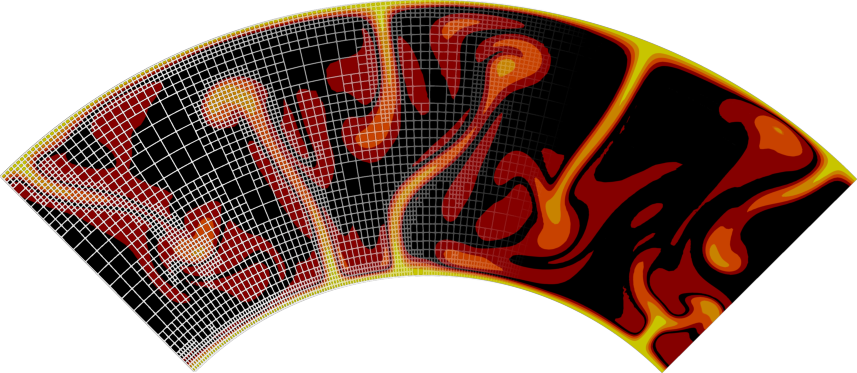
\includegraphics[width=4.5in]{../logo/unlabeled_logo.pdf}
      \hspace{5em}
    \end{center}
  \end{textblock*}

  % Then overlay some text into another textblock* environment that is
  % as wide as the page. We use \raggedright, so everything is shown
  % on the right side of the page. The y-coordinate of the anchor
  % (0.3in) is the same as for the picture, aligning the text nicely
  % to the image.
  \begin{textblock*}{\textwidth}(0in,0.3in)
    \vspace{1em}
    \color{dark_grey}
    \hfill{\Huge \fontfamily{\sfdefault}\selectfont User Manual \\
      \raggedleft \huge \fontfamily{\sfdefault}\selectfont Version
      % keep the following line as is so that we can replace this using a script:
2.5.0-pre %VERSION-INFO%
      \\
      \large(generated \today)
      \\[16pt]
        {\Large
          Wolfgang Bangerth \\
          Juliane Dannberg \\
          Menno Fraters \\
          Rene Gassm{\"o}ller \\
          Anne Glerum \\
          Timo Heister \\
          Bob Myhill \\
          John Naliboff\\}
    }
  \end{textblock*}
}


%AUTHOR(S) & WEBSITE%
\null
\vfill
\color{dark_grey}
{\fontfamily{\sfdefault}\selectfont
% FILL: author list
% e.g. Author One\\Author Two\\Author Three\\
% be sure to have a newline (\\) after the final author
\large
\noindent with contributions by: \\
    Jacqueline Austermann,
    Magali Billen,
    Markus B{\"u}rg,
    Thomas Clevenger,
    Samuel Cox,
    William Durkin,
    Grant Euen,
    Thomas Geenen,
    Ryan Grove,
    Eric Heien,
    Ludovic Jeanniot,
    Louise Kellogg,
    Scott King,
    Martin Kronbichler,
    Marine Lasbleis,
    Haoyuan Li,
    Shangxin Liu,
    Hannah Mark,
    Elvira Mulyukova,
    Bart Niday,
    Jonathan Perry-Houts,
    Elbridge Gerry Puckett,
    Tahiry Rajaonarison,
    Fred Richards,
    Jonathan Robey,
    Ian Rose,
    Max Rudolph,
    Stephanie Sparks,
    D.~Sarah Stamps,
    Cedric Thieulot,
    Wanying Wang,
    Iris van Zelst,
    Siqi Zhang\\
\vspace{0.5em}
}

{\noindent
{\fontfamily{\sfdefault}\selectfont \href{https://geodynamics.org}{geodynamics.org}}
}

%LINE%
{\noindent
\color{dark_grey}
\rule{\textwidth}{2pt}
}

}

\pagebreak
\pagenumbering{arabic}

%%%%%%%%%%%%%%%%%%%%%%%%%%%%%%
%%%   END OF CIG MANUAL COVER TEMPLATE    %%%
%%%%%%%%%%%%%%%%%%%%%%%%%%%%%%

\pagebreak

\tableofcontents

\pagebreak

\section{Introduction}

\aspect{} --- short for Advanced Solver for Problems in Earth's ConvecTion ---
is a code intended to solve the equations that describe thermally driven
convection with a focus on doing so in the context of convection in the Earth
mantle. It is developed by computational scientists all over the world
based on the following principles:
\begin{itemize}
\item \textit{Usability and extensibility:} Simulating mantle convection is a
  difficult problem characterized not only by complicated and nonlinear
  material models but, more generally, by a lack of understanding which parts
  of a much more complicated model are really necessary to simulate the
  defining features of the problem. To name just a few examples:
  \begin{itemize}
  \item Mantle convection is often solved in a spherical shell geometry, but
    the Earth is not a sphere -- its true shape on the longest length scales is
    dominated by polar oblateness, but deviations from spherical shape
    relevant to convection patterns may go down to the length scales of
    mountain belts, mid-ocean ridges or subduction trenches. Furthermore,
    processes outside the mantle like crustal depression during glaciations
    can change the geometry as well.
  \item Rocks in the mantle flow on long time scales, but on shorter time
    scales they behave more like a visco-elasto-plastic material as they break
    and as their crystalline structure heals again. The mathematical models
    discussed in Section~\ref{sec:models} can therefore only be
    approximations.
    \item If pressures are low and temperatures high enough, rocks melt,
      leading to all sorts of new and interesting behavior.
  \end{itemize}
  This uncertainty in what problem one actually wants to solve requires a code
  that is easy to extend by users to support the community in determining what
  the essential features of convection in the Earth mantle are. Achieving this
  goal also opens up possibilities outside the original scope, such as the
  simulation of convection in exoplanets or the icy satellites of the gas
  giant planets in our solar system.

\item \textit{Modern numerical methods:} We build \aspect{} on numerical
  methods that are at the forefront of research in all areas -- adaptive mesh
  refinement, linear and nonlinear solvers, stabilization of
  transport-dominated processes. This implies complexity in our algorithms,
  but also guarantees highly accurate solutions while remaining efficient in
  the number of unknowns and with CPU and memory resources.

\item \textit{Parallelism:} Many convection processes of interest are
  characterized by small features in large domains -- for example, mantle
  plumes of a few tens of kilometers diameter in a mantle almost 3,000 km
  deep. Such problems can not be solved on a single computer but require
  dozens or hundreds of processors to work together. \aspect{} is designed
  from the start to support this level of parallelism.

\item \textit{Building on others' work:} Building a code that satisfies above
  criteria from scratch would likely require several 100,000 lines of
  code. This is outside what any one group can achieve on academic time
  scales. Fortunately, most of the functionality we need is already available
  in the form of widely used, actively maintained, and well tested and
  documented libraries, and we leverage these to make \aspect{} a much smaller
  and easier to understand system. Specifically, \aspect{} builds immediately
  on top of the \dealii{} library (see \url{https://www.dealii.org/}) for
  everything that has to do with finite elements, geometries, meshes, etc.;
  and, through \dealii{} on Trilinos (see \url{http://trilinos.org/})
  for parallel linear algebra and on \pfrst{} (see
  \url{http://www.p4est.org/}) for parallel mesh handling.

\item \textit{Community:} We believe that a large project like \aspect{} can
  only be successful as a community project. Every contribution is welcome and
  we want to help you so we can improve \aspect{} together.

\end{itemize}

Combining all of these aspects into one code makes for an interesting
challenge. We hope to have achieved our goal of providing a useful tool to the
geodynamics community and beyond!


\note{\aspect{} is a community project. As such, we encourage contributions
  from the community to improve this code over time. Natural candidates for
  such contributions are implementations of new plugins as discussed in
  Section~\ref{sec:plugins-concrete} since they are typically self-contained and do not
  require much knowledge of the details of the remaining code. Obviously,
  however, we also encourage contributions to the core functionality in any
  form! If you have something that might be of general interest, please
  contact us.}

\note{\aspect{} will only solve problems relevant to the community if we get
  feedback from the community on things that are missing or necessary for what
  you want to do. Let us know by personal email to the developers, or open
  a topic on our forum hosted at
  \url{https://community.geodynamics.org/c/aspect}!}

\subsection{Referencing \aspect{}}

As with all scientific work, funding agencies have a reasonable expectation
that if we ask for continued funding for this work, we need to demonstrate
relevance.
In addition, many have contributed to the development of \aspect{} and deserve credit
for their work.
To this end, we ask that you cite the appropriate references if you
publish results that were obtained to some part using \aspect{}. For
what exactly to cite and suggestions for acknowledgments,
please see
{\bf \url{https://aspect.geodynamics.org/cite.html}}.

Also see \cite{aspect-doi-v1.5.0,aspect-doi-v2.0.0,aspect-doi-v2.0.1,aspectmanual,KHB12,heister_aspect_methods2}.


\subsection{Acknowledgments}

The development of \aspect{} has been funded
through a variety of grants to the authors. Most immediately, it has been
supported through the Computational Infrastructure in Geodynamics
(CIG), initially by the CIG-I grant (National Science Foundation Award No. EAR-0426271,
via The California Institute of Technology) and later by the CIG-II
and CIG-III grants
(National Science Foundation Awards No. EAR-0949446 and EAR-1550901, via The University
of California -- Davis). In addition, the libraries upon
which \aspect{} builds heavily have been supported through many other grants
that are equally gratefully acknowledged.

Please acknowledge CIG as follows:
{\parindent0pt
  \begin{center}
    \shadowbox{
      \begin{minipage}[c]{0.9\linewidth}
ASPECT is hosted by the Computational Infrastructure for Geodynamics (CIG)
which is supported by the National Science Foundation award EAR-1550901.
      \end{minipage}
    }
  \end{center}
}

The \aspect{} community as a whole, and a number of the primary
developers in particular, owe great thanks to Louise Kellogg
who, when she was the head of CIG, was a strong supporter of the
\aspect{} project. Louise loved how collaborative the \aspect{}
development model was, and how many people contributed. Louise passed
away far too early in 2019, but her support lives on in the spirit of
this project.


\section{Geodynamic modeling assumptions and numerical methods in \aspect{}}
\label{sec:models}

\subsection{Basic equations}
\label{sec:equations}

\aspect{} solves a system of equations in a $d=2$- or $d=3$-dimensional
domain $\Omega$ that describes the motion of a highly viscous fluid driven
by differences in the gravitational force due to a density that depends on
the temperature. In the following, we largely follow the exposition of this
material in Schubert, Turcotte and Olson \cite{STO01}.

Specifically, we consider the following set of equations for velocity $\mathbf
u$, pressure $p$ and temperature $T$, as well as a set of advected quantities
$c_i$ that we call \textit{compositional fields}:
\begin{align}
  \label{eq:stokes-1}
  -\nabla \cdot \left[2\eta \left(\varepsilon(\mathbf u)
                                  - \frac{1}{3}(\nabla \cdot \mathbf u)\mathbf 1\right)
                \right] + \nabla p &=
  \rho \mathbf g
  &
  & \textrm{in $\Omega$},
  \\
  \label{eq:stokes-2}
  \nabla \cdot (\rho \mathbf u) &= 0
  &
  & \textrm{in $\Omega$},
  \\
  \label{eq:temperature}
  \rho C_p \left(\frac{\partial T}{\partial t} + \mathbf u\cdot\nabla T\right)
  - \nabla\cdot k\nabla T
  &=
  \rho H
  \notag
  \\
  &\quad
  +
  2\eta
  \left(\varepsilon(\mathbf u) - \frac{1}{3}(\nabla \cdot \mathbf u)\mathbf 1\right)
  :
  \left(\varepsilon(\mathbf u) - \frac{1}{3}(\nabla \cdot \mathbf u)\mathbf 1\right)
  \\
  &\quad
  +\alpha T \left( \mathbf u \cdot \nabla p \right)
  \notag
  \\
  &\quad
  + \rho T \Delta S \left(\frac{\partial X}{\partial t} + \mathbf u\cdot\nabla X\right)
  &
  & \textrm{in $\Omega$},
  \notag
  \\
  \label{eq:compositional}
  \frac{\partial c_i}{\partial t} + \mathbf u\cdot\nabla c_i
  &=
  q_i
  &
  & \textrm{in $\Omega$},
  i=1\ldots C
\end{align}
where $\varepsilon(\mathbf u) = \frac{1}{2}(\nabla \mathbf u + \nabla\mathbf
u^T)$ is the symmetric gradient of the velocity (often called the
\textit{strain rate}).%
\footnote{There is no consensus in the sciences on the notation used
  for strain and strain rate. The symbols $\varepsilon$,
  $\dot\varepsilon$,  $\varepsilon(\mathbf u)$, and
  $\dot\varepsilon(\mathbf u)$, can all be found. In this manual, and
  in the code, we will consistently use $\varepsilon$ as an
  \textit{operator}, i.e., the symbol is not used on its own but only
  as applied to a field. In other words, if $\mathbf u$ is the
  velocity field, then $\varepsilon(\mathbf u) = \frac{1}{2}(\nabla
  \mathbf u + \nabla\mathbf u^T)$ will denote the strain rate. On the
  other hand, if $\mathbf d$ is the
  displacement field, then $\varepsilon(\mathbf d) = \frac{1}{2}(\nabla
  \mathbf d + \nabla\mathbf d^T)$ will denote the strain.}


In this set of equations, \eqref{eq:stokes-1} and \eqref{eq:stokes-2}
represent the compressible Stokes equations in which $\mathbf u=\mathbf
u(\mathbf x,t)$ is the velocity field and $p=p(\mathbf x,t)$ the pressure
field. Both fields depend on space $\mathbf x$ and time $t$. Fluid flow is
driven by the gravity force that acts on the fluid and that is proportional to
both the density of the fluid and the strength of the gravitational pull.

Coupled to this Stokes system is equation \eqref{eq:temperature} for the
temperature field $T=T(\mathbf x,t)$ that contains heat conduction terms as
well as advection with the flow velocity $\mathbf u$. The right hand side
terms of this equation correspond to
\begin{itemize}
\item internal heat production for example due to radioactive
  decay;
\item friction heating;
\item adiabatic compression of material;
\item phase change.
\end{itemize}
The last term of the temperature equation corresponds to
the latent heat generated or consumed in the process of phase change of material. The latent heat release
is proportional to changes in the fraction of material $X$ that has already
undergone the phase transition (also called phase function) and the change
of entropy $\Delta S$. This process applies both
to solid-state phase transitions and to melting/solidification.
Here, $\Delta S$ is positive for exothermic phase
transitions. As the phase of the material, for a given composition, depends
on the temperature and pressure, the latent heat term can be reformulated:
\begin{gather*}
\frac{\partial X}{\partial t} + \mathbf u\cdot\nabla X
=
\frac{DX}{Dt}
=
\frac{\partial X}{\partial T} \frac{DT}{Dt}
 + \frac{\partial X}{\partial p} \frac{Dp}{Dt}
=
\frac{\partial X}{\partial T}
\left(\frac{\partial T}{\partial t} + \mathbf u\cdot\nabla T
\right)
 + \frac{\partial X}{\partial p} \mathbf u\cdot\nabla p.
\end{gather*}
The last transformation results from the assumption that the flow field is
always in equilibrium and consequently $\partial p/\partial t=0$ (this is the
same assumption that underlies the fact that equation \eqref{eq:stokes-1}
does not have a term $\partial \mathbf u / \partial t$). With this
reformulation, we can rewrite \eqref{eq:temperature} in the following way in
which it is in fact implemented:
\begin{align}
  \label{eq:temperature-reformulated}
  \left(\rho C_p - \rho T \Delta S \frac{\partial X}{\partial T}\right)
  \left(\frac{\partial T}{\partial t} + \mathbf u\cdot\nabla
  T\right) - \nabla\cdot k\nabla T
  &=
  \rho H
  \notag
  \\
  &\quad
  +
  2\eta
  \left(\varepsilon(\mathbf u) - \frac{1}{3}(\nabla \cdot \mathbf u)\mathbf 1\right)
  :
  \left(\varepsilon(\mathbf u) - \frac{1}{3}(\nabla \cdot \mathbf u)\mathbf 1\right)
  \\
  &\quad
  +\alpha T \left( \mathbf u \cdot \nabla p \right)
  \notag
  \\
  &\quad
  + \rho T \Delta S \frac{\partial X}{\partial p} \mathbf u\cdot\nabla p
  & \quad & \textrm{in $\Omega$}.
  \notag
\end{align}

The last of the equations above, equation~\eqref{eq:compositional}, describes
the evolution of additional fields that are transported along with the
velocity field $\mathbf u$ and may react with each other and react to other
features of the solution, but that do not diffuse. We call these fields $c_i$
\textit{compositional fields}, although they can also be used for other
purposes than just tracking chemical compositions. We will discuss this
equation in more detail in Section~\ref{sec:compositional}.

\subsubsection{A comment on adiabatic heating}
Other codes and texts sometimes make a simplification to the adiabatic heating
term in the previous equation. If you assume the vertical component of the
gradient of the \textit{dynamic} pressure to be small compared to the gradient
of the \textit{total} pressure (in other words, the gradient is dominated by
the gradient of the hydrostatic pressure), then $ -\rho \mathbf g \approx
\nabla \mathbf{p} $, and we have the following relation (the negative sign is
due to $\mathbf g$ pointing downwards)
\begin{align*}
\alpha T \left( \mathbf u \cdot \nabla \mathbf p \right)
  & \approx -\alpha \rho T \mathbf u \cdot \mathbf g.
\end{align*}
While this simplification is possible, it is not necessary if you have access
to the total pressure. \aspect{} therefore by default implements the original
term without this simplification, but allows to simplify this term by setting
the ``\texttt{Use simplified adiabatic heating}''
\index[prmindex]{Use simplified adiabatic heating}
\index[prmindexfull]{Heating model!Adiabatic heating!Use simplified adiabatic heating}
parameter in section~\ref{parameters:Heating_20model/Adiabatic_20heating}.

\subsubsection{Boundary conditions}
Having discussed \eqref{eq:temperature}, let us come to the last one of the
original set of equations, \eqref{eq:compositional}. It describes the
motion of a set of advected quantities $c_i(\mathbf x,t),i=1\ldots C$. We call these
\textit{compositional fields} because we think of them as spatially and
temporally varying concentrations of different elements, minerals, or other
constituents of the composition of the material that convects. As such, these
fields participate actively in determining the values of the various
coefficients of these equations. On the other hand, \aspect{} also allows the
definition of material models that are independent of these compositional
fields, making them passively advected quantities. Several of the cookbooks in
Section~\ref{sec:cookbooks} consider compositional fields in this way, i.e.,
essentially as tracer quantities that only keep track of where material came
from.

These equations are
augmented by boundary conditions that can either be of Dirichlet, Neumann, or
tangential type on subsets of the boundary $\Gamma=\partial\Omega$:
\begin{align}
  \mathbf u &= 0 & \qquad &\textrm{on $\Gamma_{0,\mathbf u}$},
  \\
  \mathbf u &= \mathbf u_{\text{prescribed}} & \qquad &\textrm{on
  $\Gamma_{\text{prescribed},\mathbf u}$},
  \\
  \mathbf n \cdot \mathbf u &= 0 & \qquad &\textrm{on $\Gamma_{\parallel,\mathbf
  u}$},
  \\
  (2\eta \varepsilon(\mathbf u) -p I)\mathbf n  &= \mathbf t & \qquad
  &\textrm{on $\Gamma_{\text{traction},\mathbf u}$},
  \\
  T &= T_{\text{prescribed}}
   & \qquad &\textrm{on $\Gamma_{D,T}$},
  \\
  \mathbf n \cdot k\nabla T &= 0
   & \qquad &\textrm{on $\Gamma_{N,T}$}.
  \\
  \label{eq:gamma-in-composition}
  c_i &= c_{i,\text{prescribed}}
   & \qquad &\textrm{on $\Gamma_{\text{in}}=\{\mathbf x: \mathbf
   u\cdot\mathbf n<0\}$}.
\end{align}
Here, the boundary conditions for velocity and temperature are subdivided into
disjoint parts:
\begin{itemize}
  \item $\Gamma_{0,\mathbf u}$ corresponds to parts of the boundary on
which the velocity is fixed to be zero.
  \item $\Gamma_{\text{prescribed},\mathbf u}$ corresponds to parts of the
  boundary on which the velocity is prescribed to some value (which could also
  be zero). It is possible to restrict prescribing the velocity to only certain
  components of the velocity vector.
  \item $\Gamma_{\parallel,\mathbf u}$ corresponds to parts of the boundary on
  which the velocity may be nonzero but must be parallel to the boundary, with the
tangential component undetermined.
  \item $\Gamma_{\text{traction},\mathbf u}$ corresponds to parts of the
  boundary on which the traction is prescribed to some surface force density (a
  common application being $\mathbf t=-p\mathbf n$ if one
  just wants to prescribe a pressure component). It is possible to restrict
  prescribing the traction to only certain vector components.
  \item $\Gamma_{D,T}$ corresponds to places where the temperature is prescribed
  (for example at the inner and outer boundaries of the Earth's mantle).
  \item $\Gamma_{N,T}$ corresponds to places where the temperature is unknown
  but the heat flux across the boundary is zero (for example on symmetry surfaces if only a part
of the shell that constitutes the domain the Earth's mantle occupies is
simulated).
\end{itemize}
We require that one of these boundary conditions hold at each
point for both velocity and temperature, i.e.,
$\Gamma_{0,\mathbf u}\cup\Gamma_{{\text{prescribed}}\mathbf
  u}\cup\Gamma_{\parallel,\mathbf u}\cup\Gamma_{{\text{traction}}\mathbf
  u}=\Gamma$ and
$\Gamma_{D,T}\cup\Gamma_{N,T}=\Gamma$.

Boundary conditions have to be imposed for the compositional fields only
at those parts of the boundary where flow points inward, see equation
\eqref{eq:gamma-in-composition}, but not where it is either tangential
to the boundary or points outward. The difference in treatment between
temperature and compositional boundary conditions is due to the fact
that the temperature equation contains a (possibly small) diffusion
component, whereas the compositional equations do not.

There are other equations that \aspect{} can optionally solve. For example, it
can deal with free surfaces (see Section~\ref{sec:freesurface}), melt generation and
transport (see Section~\ref{sec:melt_transport}), and it can advect along
particles (see Section~\ref{sec:particles}). These optional models
are discussed in more detail in the indicated sections.


\subsubsection{Two-dimensional models}
\label{sec:meaning-of-2d}
\aspect{} allows solving both two- and three-dimensional
models via a parameter in the input files, see also Section~\ref{sec:2d-vs-3d}.
\index[prmindex]{Dimension} \index[prmindexfull]{Dimension}
At the same time, the world is unambiguously three-dimensional. This raises the
question what exactly we mean when we say that we want to solve two-dimensional
problems.

The notion we adopt here -- in agreement with that chosen by many other codes --
is to think of two-dimensional models in the following way: We assume that the
domain we want to solve on is a two-dimensional cross section (parameterized by
$x$ and $y$ coordinates) that extends infinitely far in both negative and
positive $z$ direction. Further, we assume that the velocity is zero in $z$
direction and that all variables have no variation in $z$ direction. As a
consequence, we ought to really think of these two-dimensional models as
three-dimensional ones in which the $z$ component of the velocity is zero and so
are all $z$ derivatives.

If one adopts this point of view, the Stokes equations
\eqref{eq:stokes-1}--\eqref{eq:stokes-2} naturally simplify in a way that allows
us to reduce the $3+1$ equations to only $2+1$, but it makes clear that the
correct description of the compressible strain rate is still
$\varepsilon(\mathbf u) - \frac{1}{3}(\nabla \cdot \mathbf u)\mathbf 1$, rather
than using a factor of $\frac{1}{2}$ for the second term. (A derivation of why
the compressible strain rate tensor has this form can be found in \cite[Section
6.5]{STO01}.)

It is interesting to realize that this compressible strain rate indeed requires
a $3\times 3$ tensor: While under the assumptions above we have
\begin{align*}
  \varepsilon(\mathbf u) =
  \begin{pmatrix}
    \tfrac{\partial u_x}{\partial x}
    &
    \tfrac 12 \tfrac{\partial u_x}{\partial y} +
    \tfrac 12 \tfrac{\partial u_y}{\partial x}
    &
    0
    \\
    \tfrac 12 \tfrac{\partial u_x}{\partial y} +
    \tfrac 12 \tfrac{\partial u_y}{\partial x}
    &
    \tfrac{\partial u_y}{\partial y}
    &
    0
    \\
    0 & 0 & 0
  \end{pmatrix}
\end{align*}
with the expected zeros in the last row and column, the full compressible strain
rate tensor reads
\begin{align*}
  \varepsilon(\mathbf u) - \frac{1}{3}(\nabla \cdot \mathbf u)\mathbf 1 =
  \begin{pmatrix}
    \tfrac 23 \tfrac{\partial u_x}{\partial x}
    - \tfrac 13 \tfrac{\partial u_y}{\partial y}
    &
    \tfrac 12 \tfrac{\partial u_x}{\partial y} +
    \tfrac 12 \tfrac{\partial u_y}{\partial x}
    &
    0
    \\
    \tfrac 12 \tfrac{\partial u_x}{\partial y} +
    \tfrac 12 \tfrac{\partial u_y}{\partial x}
    &
    \tfrac 23 \tfrac{\partial u_y}{\partial y}
    - \tfrac 13 \tfrac{\partial u_x}{\partial x}
    &
    0
    \\
    0 & 0 &
    - \tfrac 13 \tfrac{\partial u_y}{\partial y}
    - \tfrac 13 \tfrac{\partial u_x}{\partial x}
  \end{pmatrix}.
\end{align*}
The entry in the $(3,3)$ position of this tensor may be surprising. It
disappears, however, when taking the (three-dimensional) divergence of the
stress, as is done in \eqref{eq:stokes-1}, because the divergence applies the $z$ derivative to all
elements of the last row -- and the assumption above was that all $z$
derivatives are zero; consequently whatever lives in the third row of the
strain rate tensor does not matter.



\subsubsection{Comments on the final set of equations}
\aspect{} solves these equations in essentially the form stated. In
particular, the form given in \eqref{eq:stokes-1} implies that the pressure
$p$ we compute is in fact the \textit{total pressure}, i.e., the sum of
hydrostatic pressure and dynamic pressure (however, see
Section~\ref{sec:pressure-static-dyn} for more information on this, as well as
the extensive discussion of this issue in \cite{KHB12}).
Consequently, it allows the direct use of this pressure when looking up
pressure dependent material parameters.


\subsection{Coefficients}
\label{sec:coefficients}

The equations above contain a significant number of coefficients that we will
discuss in the following. In the most general form, many of these coefficients
depend nonlinearly on the solution variables pressure $p$, temperature $T$
and, in the case of the viscosity, on the strain rate $\varepsilon(\mathbf
u)$. If compositional fields $\mathfrak c=\{c_1,\ldots,c_C\}$ are present (i.e.,
if $C>0$), coefficients may also depend on them. Alternatively, they may be
parameterized as a function
of the spatial variable $\mathbf x$. \aspect{} allows both kinds of
parameterizations.

Note that below we will discuss examples of the dependence of coefficients on
other quantities; which dependence is actually implemented in the code is a
different matter. As we will discuss in Sections~\ref{sec:parameters} and
\ref{sec:extending}, some versions of these models are already implemented and
can be selected from the input parameter file; others are easy to add to
\aspect{} by providing self-contained descriptions of a set of coefficients
that the rest of the code can then use without a need for further
modifications.

Concretely, we consider the following coefficients and dependencies:
\begin{itemize}
\item \textit{The viscosity $\eta=\eta(p,T,\varepsilon(\mathbf u),\mathfrak
c,\mathbf x)$:} Units $\si{Pa . s} =
  \si{kg}\frac{1}{\si{m . s}}$.

  The viscosity is the proportionality factor that relates total forces
  (external gravity minus pressure gradients) and fluid velocities $\mathbf
  u$. The simplest models assume that $\eta$ is constant, with the constant
  often chosen to be on the order of $10^{21} \si{Pa . s}$.

  More complex (and more realistic) models assume that the viscosity depends
  on pressure, temperature and strain rate. Since this dependence is often
  difficult to quantify, one modeling approach is to make $\eta$ spatially
  dependent.

\item \textit{The density $\rho=\rho(p,T,\mathfrak c,\mathbf x)$:} Units
  $\frac{\si{kg}}{\si{m}^3}$.

  In general, the density depends on pressure and temperature, both through
  pressure compression, thermal expansion, and phase changes the material may
  undergo as it moves through the pressure-temperature phase diagram.

  The simplest parameterization for the density is to assume a linear
  dependence on temperature, yielding the form
  $\rho(T)=\rho_{\text{ref}}[1-\alpha (T-T_{\text{ref}})]$ where
  $\rho_{\text{ref}}$ is the reference density at temperature $T_{\text{ref}}$
  and $\alpha$ is the linear thermal expansion coefficient. For the earth's
  mantle, typical values for this parameterization would be
  $\rho_{\text{ref}}=3300\frac{\si{kg}}{\si{m}^3}$,
  $T_{\text{ref}}=293 \si{K}$, $\alpha=\num{2e-5}
  \frac{1}{\mathrm{K}}$.

\item \textit{The gravity vector $\mathbf g=\mathbf g(\mathbf x)$:} Units
  $\frac{\si{m}}{\textrm{s}^2}$.

  Simple models assume a radially inward gravity vector of constant magnitude
  (e.g., the surface gravity of Earth, $9.81 \frac{\si{m}}{\textrm{s}^2}$),
  or one that can be computed analytically assuming a homogeneous mantle
  density.

  A physically self-consistent model would compute the gravity vector as
  $\mathbf g = -\nabla \varphi$ with a gravity potential $\varphi$ that
  satisfies $-\Delta\varphi=4\pi G\rho$ with the density $\rho$ from above and
  $G$ the universal constant of gravity. This would provide a gravity vector
  that changes as a function of time. Such a model is not currently
  implemented.

\item \textit{The specific isobaric heat capacity $C_p=C_p(p,T,\mathfrak c,\mathbf x)$:}
Units \si{J/kg/K} = \si{m^2/s^2/K}.

  The specific heat capacity denotes the amount of energy needed to increase
  the temperature of one kilogram of material by one Kelvin at constant pressure.
  Wikipedia lists a value of
  $790 \si{J/kg/K}$ for granite%
  \footnote{See \url{http://en.wikipedia.org/wiki/Specific_heat}.}
  For the Earth's mantle, a value of $1250
  \si{J/kg/K}$ is within the range
  suggested by the literature.


\item \textit{The thermal conductivity $k=k(p,T,\mathfrak c,\mathbf x)$:} Units
  $\frac{\textrm{W}}{\si{m}\cdot\si{K}}=\frac{\si{kg}\cdot\si{m}}{\textrm{s}^3\cdot\si{K}}$.

  The thermal conductivity denotes the amount of thermal energy flowing
  through a unit area for a given temperature gradient. It depends on the
  material and as such will from a physical perspective depend on pressure and
  temperature due to phase changes of the material as well as through
  different mechanisms for heat transport (see, for example, the partial
  transparency of perovskite, the most abundant
  material in the earth mantle, at pressures above around 120 GPa
  \cite{BRVMFG04}).

  As a rule of thumb for its
  order of magnitude, Wikipedia quotes values of
  $1.83$--$2.90\frac{\textrm{W}}{\si{m}\cdot\si{K}}$ for sandstone and
  $1.73$--$3.98\frac{\textrm{W}}{\si{m}\cdot\si{K}}$ for granite.%
  \footnote{See \url{http://en.wikipedia.org/wiki/Thermal_conductivity} and
    \url{http://en.wikipedia.org/wiki/List_of_thermal_conductivities}.} The
  values in the mantle are almost certainly higher than this though probably
  not by much. The exact value is not really all that important: heat
  transport through convection is several orders of magnitude more important
  than through thermal conduction.

  The thermal conductivity $k$ is often expressed in terms of the
  \textit{thermal diffusivity} $\kappa$ using the relation $k = \rho C_p \kappa$.

\item \textit{The intrinsic specific heat production $H=H(\mathbf x)$:} Units
  $\frac{\textrm{W}}{\si{kg}}=\frac{\si{m}^2}{\textrm{s}^3}$.

  This term denotes the intrinsic heating of the material, for example due to
  the decay of radioactive material. As such, it depends not on pressure or
  temperature, but may depend on the location due to different chemical
  composition of material in the earth mantle. The literature suggests a value
  of $\gamma=\num{7.4e-12}\frac{\textrm{W}}{\si{kg}}$.

\item \textit{The thermal expansion coefficient $\alpha=\alpha(p,T,\mathfrak c ,\mathbf x)$:} Units
  $\frac{1}{\si{K}}$.

  This term denotes by how much the material under consideration
  expands due to temperature increases at constant pressure.
  This coefficient is defined as
  $\alpha = -\frac{1}{\rho} \left(\frac{\partial \rho}{\partial T}\right)_{p}$,
  where the negative sign is due the fact that the density
  \textit{decreases} as a function of temperature. Alternatively, if
  one considers the \textit{volume} $V=V(T)$ a piece of material of mass $M$
  occupies, $V=\frac{M}{\rho}$, then the thermal expansion coefficient
  is defined as the relative increase in volume,
  $\alpha=\frac{1}{V}\frac{\partial V(T)}{\partial T}$, because
  $\frac{\partial V(T)}{\partial T} =
   \frac{\partial \frac{M}{\rho}}{\partial T} =
   -\frac{M}{\rho^2} \frac{\partial \rho}{\partial T} =
   -\frac{V}{\rho} \frac{\partial \rho}{\partial T}$.

   The literature suggests that values of $\alpha=\num{1e-5}\frac{1}{\si{K}}$ at the core-mantle boundary and $\alpha=\num{4e-5}\frac{1}{\si{K}}$ are appropriate for Earth.

\item \textit{The isothermal compressibility $\beta_T=\beta_T(p,T,\mathfrak c ,\mathbf x)$:} Units
  $\frac{1}{\textrm{Pa}}$.

  This term quantifies how much the material under consideration
  contracts due to pressure increases at constant temperature.
  This coefficient is defined as
  $\beta_T = \frac{1}{\rho} \left( \frac{\partial \rho}{\partial p} \right)_{T}$.
  Alternatively, if
  one considers the \textit{volume} $V=V(p, T)$ a piece of material of mass $M$
  occupies, $V=\frac{M}{\rho}$, then the isothermal compressibility
  is defined as the relative increase in volume,
  $\beta=\frac{1}{V}\left(\frac{\partial V(p, T)}{\partial p}\right)_{T}$, because
  $\frac{\partial V(p, T)}{\partial p} =
   \frac{\partial \frac{M}{\rho}}{\partial p} =
   -\frac{M}{\rho^2} \frac{\partial \rho}{\partial p} =
   -\frac{V}{\rho} \frac{\partial \rho}{\partial p}$.

   Values of $\beta=10^{-12}$ -- $10^{-11} \frac{1}{\textrm{Pa}}$
   are reasonable for Earth's mantle, with values decreasing by about a factor of 5 between the shallow lithosphere and core-mantle boundary.

\item \textit{The isentropic/adiabatic compressibility $\beta_S=\beta_S(p,T,\mathfrak c ,\mathbf x)$:} Units
  $\frac{1}{\textrm{Pa}}$.

  This term quantifies how much the material under consideration
  contracts due to pressure increases at constant entropy.
  This coefficient is defined as
  $\beta_S = \frac{1}{\rho} \left( \frac{\partial \rho}{\partial p} \right)_{S}$.
  Alternatively, if
  one considers the \textit{volume} $V=V(p, T)$ a piece of material of mass $M$
  occupies, $V=\frac{M}{\rho}$, then the isentropic compressibility
  is defined as the relative increase in volume,
  $\beta=\frac{1}{V}\left(\frac{\partial V(p, T)}{\partial p}\right)_{S}$, because
  $\frac{\partial V(p, T)}{\partial p} =
   \frac{\partial \frac{M}{\rho}}{\partial p} =
   -\frac{M}{\rho^2} \frac{\partial \rho}{\partial p} =
   -\frac{V}{\rho} \frac{\partial \rho}{\partial p}$.
   The isentropic and isothermal compressibility are related by the expression:
   \begin{equation}
     \beta_S = \beta_T - \frac{\alpha^2 T}{\rho C_p}
   \end{equation}
   The ratio of the compressibilities decreases with increasing temperature
   and increases with increasing pressure. In the Earth's convecting mantle,
   $\beta_S/\beta_T = 0.92$--$0.98$. Different mineral assemblages have
   different values of this ratio under the same conditions. For example, the
   upper-lower boundary may exhibit a 3--4\% drop in $\beta_S / \beta_T$
   as a result of a 40\% lower $C_p$ of bridgmanite-periclase assemblages
   relative to the olivine polymorphs.


\item \textit{The change in entropy $\Delta S$ at a
  phase transition together with the derivatives of the phase function
  $X=X(p,T,\mathfrak c,\mathbf x)$ with regard to temperature and pressure:} Units
  \si{J/kg/K^2} ($-\Delta S \frac{\partial X}{\partial T}$) and
  \si{m^3/kg/K} ($\Delta S \frac{\partial X}{\partial p}$).

  When material undergoes a phase transition, the entropy changes due to
  release or consumption of latent heat. However, phase transitions occur
  gradually and for a given chemical composition it depends on temperature
  and pressure which phase prevails. Thus, the latent heat release can
  be calculated from the change of entropy $\Delta S$ and the derivatives
  of the phase function $\frac{\partial X}{\partial T}$ and
  $\frac{\partial X}{\partial p}$. These values have to be provided by
  the material model, separately for the coefficient
  $-\Delta S \frac{\partial X}{\partial T}$ on the left-hand side and
  $\Delta S \frac{\partial X}{\partial p}$ on the right-hand side of the
  temperature equation. However, they may be either approximated with the help
  of an analytic phase function, employing data from a thermodynamic database
  or in any other way that seems appropriate to the user.
\end{itemize}

\subsubsection{Coefficient self-consistency}
\label{sec:coefficient_self_consistency}
\textit{This section was contributed by Bob Myhill.}

The coefficients in the previous section may at first appear independent.
However, there are thermodynamic relations between these properties which must be
satisfied in any self-consistent material model.
The following section describes the relations required for thermodynamic
consistency, and presents some suggested ways by which consistency can be assured.

In order to derive the relationships between different material properties, we must
introduce a thermodynamic potential known as the
\href{https://en.wikipedia.org/wiki/Gibbs_free_energy}{\textit{specific
    Gibbs free energy}}
$\mathcal{G}(p, T)$ with units $\si{J}/\si{kg}$. The word ``specific'' indicates that the energy is
given per unit mass, rather than volume or number of atoms or molecules. This potential is
equal to the maximum amount of non-expansion work that can be extracted from a
thermodynamically closed system. At equilibrium conditions and fixed temperature and
pressure, the Gibbs free energy is minimized. The following equations provide the
definitions and relationships between thermodynamic properties in terms of the specific
Gibbs free energy:
\begin{eqnarray}
  S &=& - \left( \frac{\partial \mathcal{G}}{\partial T} \right)_{p}, \\
  \frac{1}{\rho} &=& \left( \frac{\partial \mathcal{G}}{\partial p} \right)_{T}, \label{eq:mm_density} \\
  \frac{\alpha}{\rho} &=& \frac{\partial^2 \mathcal{G}}{\partial {p} \, \partial {T}}, \label{eq:mm_alpha_g} \\
  \beta_T &=& -\rho \left( \frac{\partial^2 \mathcal{G}}{\partial {p}^2}  \right)_{T}, \label{eq:mm_betaT_g} \\
  C_p &=& -T \left( \frac{\partial^2 \mathcal{G}}{\partial {T}^2}  \right)_{p}, \label{eq:mm_isobaric_heat_capacity} \\
  \beta_S &=& \beta_T - \frac{\alpha^2 T}{\rho C_p}, \label{eq:mm_isentropic_compressibility} \\
  \frac{C_V}{C_p} &=& \frac{\beta_S}{\beta_T}, \\
  \gamma &=& \frac{\alpha }{\beta_T \rho C_V}.
\end{eqnarray}
where $S$ is the specific entropy, $C_p$ and $C_V$ are the specific isobaric
and isochoric heat capacities, $\beta_T$ and $\beta_S$ are the isothermal and isotropic
compressibilities, and $\gamma$ is the thermodynamic Gr\"{u}neisen parameter. The subscript
indicates the thermodynamic variable ($p$ or $T$) that is held constant.

Thermodynamically self-consistent material models must obey the explicit and implicit relations
between the different properties \emph{at all pressures and temperatures}. Explicit relations
are here defined as those between properties and their derivatives, such as that between
density and thermal expansivity. Implicit relations involve mixed pressure and temperature
derivatives, and derive from the symmetry of second derivatives. The following paragraphs
list the relations most relevant for the construction of thermodynamically-consistent material
models in \aspect{}.

\paragraph{Consistency in $\boldsymbol{\rho}$-$\boldsymbol{\alpha}$ and $\boldsymbol{\rho}$-$\boldsymbol{\beta_T}$}
Using the chain rule to combine~\eqref{eq:mm_density},~\eqref{eq:mm_alpha_g}
and~\eqref{eq:mm_betaT_g} yields the more familiar definitions of $\alpha$ and $\beta_T$:
\begin{eqnarray}
  \alpha &=& -\frac{1}{\rho} \left( \frac{\partial \rho}{\partial T} \right)_{p}, \label{eq:mm_thermal_expansivity} \\
  \beta_T &=& \frac{1}{\rho} \left( \frac{\partial \rho}{\partial p} \right)_{T}. \label{eq:mm_isothermal_compressibility}
\end{eqnarray}

\paragraph{Isobaric heat capacity}

We start by taking the partial derivative of the isobaric heat
capacity~\eqref{eq:mm_isobaric_heat_capacity} with respect to pressure at constant temperature:
\begin{eqnarray}
  \left( \frac{\partial C_p}{\partial p} \right)_{T} &=& -T \frac{\partial^3 \mathcal{G}}{\partial {T}^2 \, \partial {p}} \\
  &=& -T \left( \frac{\partial \left(\alpha / \rho \right)}{\partial T} \right)_{p}. \label{eq:heat_capacity_p_dependence}
\end{eqnarray}
From this expression it becomes clear that if $\alpha / \rho$ has any temperature dependence,
the heat capacity $C_p$ \emph{cannot} be globally constant. One way to solve this issue is to define
heat capacity at constant pressure, and then integrate~\eqref{eq:heat_capacity_p_dependence}
with respect to pressure:
\begin{equation}
  C_p(p, T)
  = C_p(p_{\textrm{ref}}, T) -T \int_{p_{\textrm{ref}}}^p
  \left(\frac{\partial \left(\alpha / \rho \right)}{\partial T} \right)_{p}
  \text{d}p.
\end{equation}
There is no guarantee that this expression will have a form for which the integral can be found analytically.

\paragraph{Isentropic gradient}
The material properties also define the slope of the adiabat (the change in temperature with
pressure at constant entropy) at all pressures and temperatures. Using the cyclic relation,
we can define this slope in terms of partial differentials of the entropy with respect to pressure
and temperature:
\begin{eqnarray}
  \left( \frac{\partial T}{\partial p} \right)_{S} &=& - \left( \frac{\partial T}{\partial S} \right)_{p} \left( \frac{\partial S}{\partial p} \right)_{T} \\
  &=& - \left( \frac{T}{C_p} \right) \left( - \frac{\alpha}{\rho} \right) \\
  &=& \frac{\alpha T}{\rho C_p} \label{eq:mm_isentropic_gradient}
\end{eqnarray}
This expression does not pose a constraint on the material properties, but in order to be
self-consistent, the adiabat must be computed following this relation.

For complex material models, obtaining analytical functions which obey all these relations
may be a non-trivial exercise. Furthermore, it is often not immediately clear when a
given formulation is thermodynamically inconsistent. Indeed, both the
thermodynamic and the geodynamic literature contain many equations of
state and material parameterizations which do not obey these
relations! This may not invalidate the results obtained with these
models, but it is a point worth keeping in mind as the geodynamics
community moves to more complicated and more realistic parameterizations.

\emph{A final note of warning: Some compressible formulations in \aspect{}
  (Section~\ref{sec:mass-conservation-approximation}) use the isothermal compressibility,
  while others use the isentropic compressibility. Fully self-consistent material models must
  either specify what approximation of the compressible equations they are consistent with
  (see Section~\ref{sec:approximate-equations}), or have a switch so that they use the correct
  compressibility for each of the different approximations. The conversion between isothermal
  and isentropic compressibilities is given in~\eqref{eq:mm_isentropic_compressibility}.}


\subsubsection{Coefficient averaging}
In multiphase rocks, or multirock areas in convection simulations, properties must be averaged
because the length scales at which the rock types vary is far smaller than the resolution of the mesh.
As a consequence, we need to use ``effective coefficients'', i.e., coefficients that do not
correspond to any particular rock, but that lead to a macroscopic response that is a good match
to the response of the correct, but unresolvable mixture of rocks.
For viscosity and conductivity, there is no single expression that describes how averaging should
be performed; indeed, these properties are dependent on rock texture and mineral alignment,
both of which may change through time as strain accumulates, and chemical diffusion and
reactions take place. Some of the existing multicomponent material models in \aspect{} allow the
user to choose from a range of averaging schemes for viscosity.

In the case of density, thermal expansivity, heat capacity and bulk compressibility, there is
one correct way of averaging. Here we must consider conservation of mass and composition in a
multicomponent rock $r$. If component $i$ has masses $M_i$ and densities $\rho_i$, we
can consider the summation of volume fractions:
\begin{eqnarray}
  V_r &=& \frac{M_r}{\rho_r} = \sum_i \frac{M_i}{\rho_i} \\
  \frac{1}{\rho_r} &=& \sum_i \frac{x_i}{\rho_i}
\end{eqnarray}
where $x_i$ are mass fractions of the components in the rock.

Similarly, we can obtain averaging formulae for the other thermodynamic properties:
\begin{eqnarray}
  \frac{\alpha}{\rho} &=& \sum_i x_i \frac{\alpha_i}{\rho_{i}} \\
  \frac{\beta_T}{\rho} &=& \sum_i x_i \frac{\beta_{Ti}}{\rho_{i}} \\
  C_p &=& \sum_i x_i C_{pi}
\end{eqnarray}



\subsection{Dimensional or non-dimensionalized equations?}
\label{sec:non-dimensional}

Equations \eqref{eq:stokes-1}--\eqref{eq:temperature} are stated in their
physically correct form. One would usually interpret them in a way that the
various coefficients such as the viscosity, density and thermal conductivity
$\eta,\rho,\kappa$ are given in their correct physical units, typically
expressed in a system such as the meter, kilogram, second (MKS) system that is
part of the \href{http://en.wikipedia.org/wiki/SI}{SI} system.
This is certainly how we envision \aspect{} to be used: with geometries,
material models, boundary conditions and initial values to be given in their correct
physical units. As a consequence, when \aspect{} prints information about the
simulation onto the screen, it typically does so by using a postfix such as
\texttt{m/s} to indicate a velocity or \texttt{W/m\^{}2} to indicate a heat
flux.

\note{For mantle convection simulations, it is often convenient to work with
time units of \textit{years} instead of \textit{seconds}. The flag
``\texttt{Use years in output instead of seconds}'' (Section~\ref{parameters:global})
in the input file determines how input and output parameters with units of time or
velocity are interpreted. For details, see Section~\ref{sec:years-or-seconds} below.}

That said, in reality, \aspect{} has no preferred system of
units as long as every material constant, geometry, time, etc., are all
expressed in the same system. In other words, it is entirely legitimate to
implement geometry and material models in which the dimension of the domain is
one, density and viscosity are one, and the density variation as a function of
temperature is scaled by the Rayleigh number -- i.e., to use the usual
non-dimensionalization of the equations~\eqref{eq:stokes-1}--\eqref{eq:temperature}. Some of the cookbooks in
Section~\ref{sec:cookbooks} use this non-dimensional form; for example,
the simplest cookbook in Section~\ref{sec:cookbooks-simple-box} as well as
the SolCx, SolKz and inclusion benchmarks in Sections~\ref{sec:benchmark-solcx},
are such cases. Whenever this is the case, output showing units \texttt{m/s} or
\texttt{W/m\^{}2} clearly no longer have a literal meaning. Rather, the unit postfix must in this case simply
be interpreted to mean that the number that precedes the first is a velocity and
a heat flux in the second case.

In other words, whether a computation uses physical or non-dimensional units
really depends on the geometry, material, initial and boundary condition
description of the particular case under consideration -- \aspect{} will simply
use whatever it is given. Whether one or the other is the more appropriate
description is a decision we purposefully leave to the user. There are of
course good reasons to use non-dimensional descriptions of realistic problems,
rather than to use the original form in which all coefficients remain in their
physical units. On the other hand, there are also downsides:
\begin{itemize}
  \item Non-dimensional descriptions, such as when using the
  \href{http://en.wikipedia.org/wiki/Rayleigh_number}{Rayleigh} number to
  indicate the relative strength of convective to diffusive thermal transport,
  have the advantage that they allow to reduce a system to its essence. For
  example, it is clear that we get the same behavior if one increases both the
  viscosity and the thermal expansion coefficient by a factor of two because the
  resulting Rayleigh number; similarly, if we were to increase the size of the
  domain by a factor of 2 and thermal diffusion coefficient by a factor of 8. In both of
  these cases, the non-dimensional equations are exactly the same. On the other
  hand, the equations in their physical unit form are different and one may not
  see that the result of this variations in coefficients will be exactly the
  same as before. Using non-dimensional variables therefore reduces the space of
  independent parameters one may have to consider when doing parameter studies.

  \item From a practical perspective, equations
  \eqref{eq:stokes-1}--\eqref{eq:temperature} are often ill-conditioned in
  their original form: the two sides of each equation have physical units
  different from those of the other equations, and their numerical values are
  often vastly different.%
  \footnote{To illustrate this, consider convection in the Earth as a
  back-of-the-envelope example.
  With the length scale of the mantle $L=\num{3e6}\;\si{m}$, viscosity
  $\eta=10^{24} \; \si{kg}/\si{m}/\si{s}$, density $\rho=\num{3e3} \; \si{kg}/\si{m}^3$ and a typical
  velocity of $U=0.1\;\si{m}/\text{year}=\num{3e-9}\; \si{m}/\si{s}$, we get that the friction
  term in \eqref{eq:stokes-1} has size $\eta U/L^2 \approx \num{3e2} \;
  \si{kg}/\si{m}^2/\si{s}^2$. On the other hand, the term $\nabla\cdot(\rho u)$ in the
  continuity equation \eqref{eq:stokes-2} has size $\rho U/L\approx \num{3e-12} \; \si{kg}/\si{s}/\si{m}^3$. In other words, their \textit{numerical values} are 14
  orders of magnitude apart.}
  Of course, these values can not be compared: they have different physical
  units, and the ratios between these values depends on whether we choose to
  measure lengths in meters or kilometers, for example. Nevertheless, when
  implementing these equations in software, at one point or another, we have to
  work with numbers and at this point the physical units are lost. If one does
  not take care at this point, it is easy to get software in which all accuracy
  is lost due to round-off errors. On the other hand, non-dimensionalization
  typically avoids this since it normalizes all quantities so that values that
  appear in computations are typically on the order of one.

  \item On the downside, the numbers non-dimensionalized equations produce are
  not immediately comparable to ones we know from physical experiments. This is
  of little concern if all we have to do is convert every output number of our
  program back to physical units. On the other hand, it is more difficult and a
  source of many errors if this has to be done inside the program, for example,
  when looking up the viscosity as a pressure-, temperature- and
  strain-rate-dependent function: one first has to convert pressure,
  temperature and strain rate from non-dimensional to physical units, look up
  the corresponding viscosity in a table, and then convert the viscosity back to
  non-dimensional quantities. Getting this right at every one of the dozens or
  hundreds of places inside a program and using the correct (but distinct)
  conversion factors for each of these quantities is both a challenge and a possible source
  of errors.

  \item From a mathematical viewpoint, it is typically clear how an equation
  needs to be non-dimensionalized if all coefficients are constant. However, how
  is one to normalize the equations if, as is the case in the earth mantle, the
  viscosity varies by several orders of magnitude? In cases like these, one has
  to choose a reference viscosity, density, etc. While the resulting
  non-dimensionalization retains the universality of parameters in the
  equations, as discussed above, it is not entirely clear that this would also
  retain the numerical stability if the reference values are poorly chosen.
\end{itemize}

As a consequence of such considerations, most codes in the past have used
non-dimensionalized models. This was aided by the fact that until recently and
with notable exceptions, many models had constant coefficients and the
difficulties associated with variable coefficients were not a concern. On the
other hand, our goal with \aspect{} is for it to be a code that solves realistic
problems using complex models and that is easy to use. Thus, we allow users to
input models in physical or non-dimensional units, at their discretion. We
believe that this makes the description of realistic models simpler. On
the other hand, ensuring numerical stability is not something users should have
to be concerned about, and is taken care of in the implementation of \aspect{}'s
core (see the corresponding section in \cite{KHB12}).

\subsubsection{Years or seconds?}
\label{sec:years-or-seconds}

All internal calculations in \aspect{} are performed using time units of seconds.
Input quantities with units of time or velocity are assumed to be in
seconds or meters per second, and output quantities with units of time or velocity
will also be in seconds or meters per second, unless the input parameter
\texttt{Use years in output instead of seconds} is \texttt{true}
(see Section~\ref{parameters:global}).

This parameter is somewhat deceptively named, as it influences how \aspect{}
treats inputs as well as outputs. For example, if \texttt{Use years in output instead
of seconds} is \texttt{true}, input values for \texttt{Start time},
\texttt{End time}, and \texttt{Maximum time step} are assumed to be in years
instead of seconds. When the flag is set, \aspect{} converts input time and velocity
units to MKS internally, computes solutions, and converts time and velocity outputs
back to years and meters per year during postprocessing.

By default, \texttt{Use years in output instead of seconds} is \texttt{true},
since \aspect{} is designed primarily for models described in physical units rather
than in non-dimensionalized form, and years are often more intuitive time units
for mantle convection problems (see Section~\ref{sec:non-dimensional}). For non-
dimensional models the flag should be set to \texttt{false} since conversions
between years and seconds do not make sense for non-dimensional quantities.

\subsection{Static or dynamic pressure?}
\label{sec:pressure-static-dyn}

One could reformulate equation \eqref{eq:stokes-1} somewhat. To this end, let us
say that we would want to represent the pressure $p$ as the sum of two parts
that we will call static and dynamic, $p=p_s+p_d$. If we assume that $p_s$ is
already given, then we can replace \eqref{eq:stokes-1} by
\begin{gather*}
  -\nabla \cdot 2\eta
  \nabla \mathbf u + \nabla p_d =
  \rho\mathbf g - \nabla p_s.
\end{gather*}
One typically chooses $p_s$ as the pressure one would get if the whole medium
were at rest -- i.e., as the hydrostatic pressure. This pressure can be
computed noting that \eqref{eq:stokes-1} reduces to
\begin{gather*}
  \nabla p_s = \rho(p_s,T_s,\mathbf x)\mathbf g = \bar\rho \mathbf g
\end{gather*}
in the absence of any motion where $T_s$ is some static temperature field (see
also Section~\ref{sec:adiabatic}). This, our rewritten version of
\eqref{eq:stokes-1} would look like this:
\begin{gather*}
  -\nabla \cdot 2\eta
  \nabla \mathbf u + \nabla p_d =
  \left[\rho(p,T,\mathbf x)-\rho(p_s,T_s,\mathbf x)\right]\mathbf g.
\end{gather*}
In this
formulation, it is clear that the quantity that drives the fluid flow is in
fact the \textit{buoyancy} caused by the \textit{variation} of densities,
not the density itself.

This reformulation has a number of advantages and disadvantages:
\begin{itemize}
\item One can notice that in many realistic cases, the dynamic component $p_d$
  of the pressure is orders of magnitude smaller than the static component
  $p_s$. For example, in the earth, the two are separated by around 6 orders
  of magnitude at the bottom of the earth mantle. Consequently, if one wants
  to solve the linear system that arises from discretization of the original
  equations, one has to solve it a significant degree of accuracy (6--7
  digits) to get the dynamic part of the pressure correct to even one
  digit. This entails a very significant numerical effort, and one that is not
  necessary if we can split the pressure in a way so that the pre-computed
  static pressure $p_s$ (or, rather, the density using the static pressure and
  temperature from which $p_s$ results) absorbs the dominant part and one only
  has to compute the remaining, dynamic pressure to 2 or 3 digits of accuracy,
  rather than the corresponding 7--8 for the total pressure.

\item On the other hand, the pressure $p_d$ one computes this way is not immediately
  comparable to quantities that we use to look up pressure-dependent
  quantities such as the density. Rather, one needs to first find the static
  pressure as well (see Section~\ref{sec:adiabatic}) and add the two together
  before they can be used to look up material properties or to compare them with
  experimental results. Consequently, if the pressure a program outputs
  (either for visualization, or in the internal interfaces to parts of the
  code where users can implement pressure- and temperature-dependent material
  properties) is only the dynamic component, then all of the consumers of this
  information need to convert it into the total pressure when comparing with
  physical experiments. Since any code implementing realistic material models
  has a great many of these places, there is a large potential for inadvertent
  errors and bugs.

\item Finally, the definition of a reference density $\rho(p_s,T_s,\mathbf x)$
  derived from static pressures and temperatures
  is only simple if we have incompressible models and under the assumption
  that the temperature-induced density variations are small compared to the
  overall density. In this case, we can choose $\rho(p_s,T_s,\mathbf
  x)=\rho_0$ with a constant reference density $\rho_0$. On the other hand,
  for more complicated models, it is not a priori
  clear which density to choose since we first need to compute static
  pressures and temperatures -- quantities that satisfy equations that
  introduce boundary layers, may include phase changes releasing latent heat,
  and where the density may have discontinuities at certain depths, see
  Section~\ref{sec:adiabatic}.

  Thus, if we compute adiabatic pressures and
  temperatures $\bar p_s,\bar T_s$ under the assumption of a thermal boundary layer
  worth 900 Kelvin at the top, and we get a corresponding density profile
  $\bar\rho=\rho(\bar p_s,\bar T_s, \mathbf x)$, but after running for a few
  million years the temperature turns out to be so that the top boundary layer
  has a jump of only 800 Kelvin with corresponding adiabatic pressures and
  temperatures $\hat p_s,\hat T_s$, then a more appropriate density profile
  would be $\hat\rho=\rho(\hat p_s,\hat T_s, \mathbf x)$.

  The problem is that it may well be that the erroneously computed density
  profile $\hat \rho$ does \textit{not} lead to a separation where
  $|p_d|\ll|p_s|$ because, especially if the material undergoes phase changes,
  there will be entire areas of the computational domain in which $|\rho-\hat
  \rho_s|\ll |\rho|$ but $|\rho-\bar
  \rho_s|\not\ll |\rho|$. Consequently the benefits of lesser requirements on the
  iterative linear solver would not be realized.
\end{itemize}

We do note that most of the codes available today and that we are aware of
split the pressure into static and dynamic parts nevertheless, either
internally or require the user to specify the density profile as the
difference between the true and the hydrostatic density. This may, in part, be
due to the fact that historically most codes were written to solve problems
in which the medium was considered incompressible, i.e., where the definition
of a static density was simple.

On the other hand, we intend \aspect{} to be a code that can solve more
general models for which this definition is not as simple. As a consequence, we
have chosen to solve the equations as stated originally -- i.e., we solve for
the \textit{full} pressure rather than just its \textit{dynamic} component. With
most traditional methods, this would lead to a catastrophic loss of accuracy in the
dynamic pressure since it is many orders of magnitude smaller than the total
pressure at the bottom of the earth mantle. We avoid this problem in \aspect{}
by using a cleverly chosen iterative solver that ensures that the full pressure
we compute is accurate enough so that the dynamic pressure can be extracted from
it with the same accuracy one would get if one were to solve for only the
dynamic component. The methods that ensure this are described in detail in
\cite{KHB12} and in particular in the appendix of that paper.

\note{By default, \aspect{} uses the full pressure in the equations, and only prescribing
density deviations from a reference state on the right-hand side of \eqref{eq:stokes-1}
would lead to negative densities in the energy equation \eqref{eq:temperature}.
However, when using one of the approximations described in Section \ref{sec:approximate-equations},
the energy balance uses the reference density $\bar\rho$ instead of the full density,
which makes it possible to formulate the Stokes system in terms of the dynamic instead of
the full pressure. In order to do this, one would have to use a material model
(see Section~\ref{sec:material-models}) in which the density is in fact a density variation,
and then the pressure solution variable would only be the dynamic pressure.}

\subsection{Pressure normalization}
\label{sec:pressure}

The equations described above, \eqref{eq:stokes-1}--\eqref{eq:temperature},
only determine the pressure $p$ up to an additive constant. On the other hand,
since the pressure appears in the definition of many of the coefficients, we
need a pressure that has some sort of \textit{absolute} definition. A
physically useful definition would be to normalize the pressure in such a way
that the average pressure along the ``surface'' has a prescribed value where
the geometry description (see Section~\ref{sec:geometry-models}) has to
determine which part of the boundary of the domain is the ``surface'' (we call
a part of the boundary the ``surface'' if its depth is ``close to zero'').

Typically, one will choose this average pressure to be zero, but there is a
parameter ``\texttt{Surface pressure}''
\index[prmindex]{Surface pressure}
\index[prmindexfull]{Surface pressure}
in the input file (see Section~\ref{parameters:global}) to set it to
a different value. One may want to do that, for example, if one wants to
simulate the earth mantle without the overlying lithosphere. In that case, the
``surface'' would be the interface between mantle and lithosphere, and the
average pressure at the surface to which the solution of the equations will be
normalized should in this case be the hydrostatic pressure at the bottom of
the lithosphere.

An alternative is to normalize the pressure in such a way that the
\textit{average} pressure throughout the domain is zero or some constant
value. This is not a useful approach for most geodynamics applications but is
common in benchmarks for which analytic solutions are available. Which kind of
normalization is chosen is determined by the ``\texttt{Pressure
  normalization}'' flag in the input file,
\index[prmindex]{Pressure normalization}
\index[prmindexfull]{Pressure normalization}
see Section~\ref{parameters:global}.


\subsection{Initial conditions and the adiabatic pressure/temperature}
\label{sec:adiabatic}

Equations \eqref{eq:stokes-1}--\eqref{eq:temperature} require us to
pose initial conditions for the temperature, and this is done by
selecting one of the existing models for initial conditions in the
input parameter file, see
Section~\ref{parameters:Initial_20temperature_20model}. The equations
themselves do not require that initial conditions are specified for
the velocity and pressure variables (since there are no time
derivatives on these variables in the model).

Nevertheless, a nonlinear solver will have difficulty converging to
the correct solution if we start with a completely unphysical pressure
for models in which coefficients such as density $\rho$ and viscosity
$\eta$ depend on the pressure and temperature. To this end, \aspect{}
uses pressure and temperature fields $p_{\textrm{ad}}(z),
T_{\textrm{ad}}(z)$ computed in the adiabatic conditions model
(see Section~\ref{parameters:Adiabatic_20conditions_20model}).
By default, these fields satisfy adiabatic conditions:
\begin{align}
  \rho C_p \frac{\textrm{d}}{\textrm{d}z} T_{\textrm{ad}}(z)
  &=
  \frac{\partial\rho}{\partial T} T_{\textrm{ad}}(z) g_z,
\\
  \frac{\textrm{d}}{\textrm{d}z} p_{\textrm{ad}}(z)
  &=
  \rho g_z,
\end{align}
where strictly speaking $g_z$ is the magnitude of the vertical
component of the gravity vector field, but in practice we take the
magnitude of the entire gravity vector.

These equations can be integrated numerically starting at $z=0$, using
the depth dependent gravity field and values of the coefficients
$\rho=\rho(p,T,z), C_p=C_p(p,T,z)$. As starting conditions at $z=0$ we
choose a pressure $p_{\textrm{ad}}(0)$ equal to the average surface
pressure (often chosen to be zero, see Section~\ref{sec:pressure}),
and an adiabatic surface temperature $T_{\textrm{ad}}(0)$ that is
\index[prmindex]{Adiabatic surface temperature}
\index[prmindexfull]{Adiabatic surface temperature}
also selected in the input parameter file.

However, users can also supply their own adiabatic conditions models or
define an arbitrary profile using the ``function'' plugin.

\note{The adiabatic surface temperature is often chosen significantly
  higher than the actual surface temperature. For example, on earth,
  the actual surface temperature is on the order of 290 K, whereas a
  reasonable adiabatic surface temperature is maybe 1600 K. The reason
  is that the bulk of the mantle is more or less in thermal equilibrium
  with a thermal profile that corresponds to the latter temperature,
  whereas the very low actual surface temperature and the very high
  bottom temperature at the core-mantle boundary simply induce a
  thermal boundary layer. Since the temperature and pressure profile
  we compute using the equations above are simply meant to be good
  starting points for nonlinear solvers, it is important to choose
  this profile in such a way that it covers most of the mantle well;
  choosing an adiabatic surface temperature of 290 K would yield a
  temperature and pressure profile that is wrong almost throughout the
  entire mantle.}



\subsection{Compositional fields}
\label{sec:compositional}

The last of the basic equations, \eqref{eq:compositional}, describes the
evolution of a set of variables $c_i(\mathbf x, t), i=1\ldots C$ that we
typically call \textit{compositional fields} and that we often aggregate into
a vector $\mathfrak c$.

Compositional fields were originally intended to track what their name
suggest, namely the chemical composition of the convecting medium. In this
interpretation, the composition is a non-diffusive quantity that is simply advected along
passively, i.e., it would satisfy the equation
\begin{align*}
  \frac{\partial \mathfrak c}{\partial t} + \mathbf u \cdot \nabla \mathfrak c
  = 0.
\end{align*}
However, the compositional fields may also participate in determining the values of
the various coefficients as discussed in
Section~\ref{sec:coefficients}, and in this sense the equation above
describes a composition that is \textit{passively advected}, but an
\textit{active participant} in the equations.

That said, over time compositional fields have shown to be a much more useful
tool than originally intended. For example, they can be used to track where
material comes from and goes to (see Section~\ref{sec:cookbooks-composition})
and, if one allows for a reaction rate $\mathfrak q$ on the right hand side,
\begin{align*}
  \frac{\partial \mathfrak c}{\partial t} + \mathbf u \cdot \nabla \mathfrak c
  = \mathfrak q,
\end{align*}
then one can also model interaction between species -- for example to simulate
phase changes where one compositional field, indicating a particular phase,
transforms into another phase depending on pressure and temperature, or where
several phases combine to other phases. Another example of using a
right hand side -- quite outside what the original term
\textit{compositional field} was supposed to indicate -- is to track
the accumulation of finite strain, see Section~\ref{sec:finite-strain}.

In actual practice, one finds that it is often useful to allow
$\mathfrak q$ to be a function that has both a smooth (say,
continuous) in time component, and one that is singular in time (i.e.,
contains Dirac delta, or ``impulse'' functions). Typical time
integrators require the evaluation of the right hand side at specific
points in time, but this would preclude the use of delta
functions. Consequently, the integrators in \aspect{} only require
material models to provide an \textit{integrated} value
$\int_t^{t+\Delta t} \mathfrak q(\tau) \;
\text{d}\tau$ through the {\tt reaction\_term} output
variable. Implementations often approximate this as $\triangle t \cdot
\mathfrak q(t)$, or similar formulas.

A second application for only providing integrated right hand sides
comes from the fact that
modeling reactions between different compositional fields often involves
finding an equilibrium state between different fields because
chemical reactions happen on a much faster time scale than transport. In other
words, one then often assumes that there is a $\mathfrak c^\ast(p,T)$ so that
\begin{align*}
  \mathfrak q(p,T,\varepsilon(\mathbf u),\mathfrak c^\ast(p,T)) = 0.
\end{align*}
Consequently, the material model methods that deal with source terms for the
compositional fields need to compute an \textit{increment} $\Delta\mathfrak c$
to the previous value of the compositional fields so that the sum of the
previous values and the increment equals $\mathfrak c^\ast$. This
corresponds to an \textit{impulse change} in the compositions at every
time step, as opposed
to the usual approach of evaluating the right hand side term
$\mathfrak q$ as a continuous function in time,
which corresponds to a \textit{rate}.

On the other hand, there are other uses of compositional fields that do not
actually have anything to do with quantities that can be considered related to
compositions. For example, one may define a field that tracks the grain size
of rocks. If the strain rate is high, then the grain size decreases as the
rocks break. If the temperature is high enough, then grains heal and their size
increases again. Such ``damage models'' would then introduce a
quantity $c(t)$ describing the ``damage'' to the material (here
assumed to be described by a single scalar field) that 
satisfies an equation of the form
\begin{align*}
  \frac{\partial c}{\partial t} + \mathbf u \cdot \nabla c
  = q(T,c),
\end{align*}
where in the simplest case (much simplified from real models) one
could postulate
\begin{align*}
  q(T,c) =  A \dot\varepsilon - B \max\{T-T_{\text{healing}},0\} c.
\end{align*}
Here, $\dot\varepsilon$ is the strain rate that causes damage; the
first term then leads to growth of damage as strain continues to
accumulate on the material. The second term \textit{decreases} the
damage if the temperature is high enough.
One would then use this compositional field in the definition of the viscosity
of the material: more damage means lower viscosity because the rocks are weaker.

In cases like this, there is only a single compositional field and it is not
in permanent equilibrium. Consequently, the increment implementations of
material models in \aspect{} need to compute is typically the rate $q(T,c)$
times the time step.  In other words, if you compute a reaction rate inside the material model you need to multiply it by the time step size before returning the value.

Compositional fields have proven to be surprisingly versatile tools to model
all sorts of components of models that go beyond the simple Stokes plus
temperature set of equations. Play with them!

\note{As has hopefully become clear from the discussion above, the
  term ``compositional field'' as used in \aspect{} is by now mostly
  historic: These fields were meant to track chemical compositions, but
  are now used to track all sorts of other things as well, or in some
  cases track nothing at all and just be static fields that
simply indicate where some
  features of the model are located.

  It is therefore useful to think of the term ``compositional field''
  as a \textit{technical term} in which the two words appear
  together, separate from the original meaning of the word
  ``compositional''.}


\subsection{Constitutive laws}

Equation \eqref{eq:stokes-1} describes buoyancy-driven flow in an isotropic
fluid where strain rate is related to stress by a scalar (possibly spatially variable)
multiplier, $\eta$. For some material models it is useful to generalize this
relationship to anisotropic materials, or other exotic constitutive laws.
For these cases \aspect{} can optionally include a generalized, fourth-order
tensor field as a material model state variable which changes equation
\eqref{eq:stokes-1} to
\begin{align}
  \label{eq:stokes-1-anisotropic}
  -\nabla \cdot \left[2\eta \left(C \varepsilon(\mathbf u)
                                  - \frac{1}{3}(tr(C \varepsilon(\mathbf u)))\mathbf 1\right)
                \right] + \nabla p &=
  \rho \mathbf g
  & \qquad
  & \textrm{in $\Omega$}
\end{align}
and the shear heating term in equation \eqref{eq:temperature} to
\begin{align}
  \label {eq:temperature-anisotropic}
  \dots
  \notag
  \\
  + 2 \eta
  \left(C \varepsilon(\mathbf u) - \frac{1}{3}(tr(C \varepsilon(\mathbf u)))\mathbf 1\right)
  :
  \left(\varepsilon(\mathbf u) - \frac{1}{3}(\nabla \cdot \mathbf u)\mathbf 1\right)
  \\
  \dots
  \notag
\end{align}
where $C = C_{ijkl}$ is defined by the material model. For physical reasons, $C$ needs
to be a symmetric rank-4 tensor: i.e., when multiplied by a symmetric (strain rate)
tensor of rank 2 it needs to return another symmetric tensor of rank 2. In mathematical
terms, this means that $C_{ijkl}=C_{jikl}=C_{ijlk}=C_{jilk}$. Energy considerations
also require that $C$ is positive definite: i.e., for any $\varepsilon \neq 0$, the
scalar $\varepsilon : (C \varepsilon)$ must be positive.

This functionality can be optionally invoked by any material model that chooses to
define a $C$ field, and falls back to the default case ($C=\mathbb I$) if no such
field is defined. It should be noted that $\eta$ still appears in equations
\eqref{eq:stokes-1-anisotropic} and \eqref{eq:temperature-anisotropic}. $C$ is
therefore intended to be thought of as a ``director'' tensor rather than a
replacement for the viscosity field, although in practice either interpretation
is okay.


\subsection{Numerical methods}

There is no shortage in the literature for methods to solve the equations
outlined above. The methods used by \aspect{} use the following,
interconnected set of strategies in the implementation of numerical
algorithms:
\begin{itemize}
\item \textit{Mesh adaptation:} Mantle convection problems are characterized
  by widely disparate length scales (from plate boundaries on the order of
  kilometers or even smaller, to the scale of the entire earth). Uniform
  meshes can not resolve the smallest length scale without an intractable
  number of unknowns.  Fully adaptive meshes allow resolving local features of
  the flow field without the need to refine the mesh globally. Since the
  location of plumes that require high resolution change and move with time,
  meshes also need to be adapted every few time steps.
\item \textit{Accurate discretizations:} The equations upon which
  most models for the earth mantle are based
  have a number of intricacies that make the choice of discretization
  non-trivial. In particular, the finite elements chosen for velocity and
  pressure need to satisfy the usual compatibility condition for saddle point
  problems. This can be worked around using pressure stabilization schemes for
  low-order discretizations, but high-order methods can yield better accuracy
  with fewer unknowns and offer more reliability. Equally important is the choice of
  a stabilization method for the highly advection-dominated temperature
  equation. \aspect{} uses a nonlinear artificial diffusion method for the latter.
\item \textit{Efficient linear solvers:} The major obstacle in solving the
  system of linear equations that results from discretization is the
  saddle-point nature of the Stokes equations.
  Simple linear solvers and preconditioners can not efficiently solve this system in
  the presence of strong heterogeneities or when the size of the system
  becomes very large. \aspect{} uses an efficient solution strategy based on a
  block triangular preconditioner utilizing an algebraic multigrid that
  provides optimal complexity even up to problems with hundreds of millions of
  unknowns.
\item \textit{Parallelization of all of the steps above:} Global mantle convection
  problems frequently require extremely large numbers of unknowns for
  adequate resolution in three dimensional simulations. The only realistic way to solve such problems lies in
  parallelizing computations over hundreds or thousands of processors. This is
  made more complicated by the use of dynamically changing meshes, and it
  needs to take into account that we want to retain the optimal complexity of
  linear solvers and all other operations in the program.
\item \textit{Modularity of the code:} A code that implements all of these
  methods from \textit{scratch} will be unwieldy, unreadable and unusable as a community
  resource. To avoid this, we build our implementation on widely used and well
  tested libraries that can provide researchers interested in extending it
  with the support of a large user community. Specifically, we use the
  \dealii{} library \cite{BHK07,BK99m} for meshes, finite
  elements and everything discretization related; the \trilinos{} library
  \cite{trilinos,trilinos-web-page} for scalable and parallel linear algebra;
  and \pfrst{} \cite{p4est} for distributed, adaptive meshes. As a
  consequence, our code is freed of the mundane tasks of defining finite
  element shape functions or dealing with the data structures of linear algebra,
  can focus on the high-level description of what is supposed to happen, and
  remains relatively compact. The code will also
  automatically benefit from improvements to the underlying libraries with
  their much larger development communities. \aspect{} is extensively
  documented to enable other researchers to understand, test, use, and extend it.
\end{itemize}

Rather than detailing the various techniques upon which \aspect{} is built, we
refer to the papers by Kronbichler, Heister and Bangerth \cite{KHB12}
and Heister, Dannberg, Gassm{\"o}ller and Bangerth \cite{heister_aspect_methods2}
that
give a detailed description and rationale for the various building blocks.


\subsection{Approximate equations}
\label{sec:approximate-equations}

There are a number of common variations to equations
\eqref{eq:stokes-1}--\eqref{eq:temperature} that are used in the
geosciences. For example, one frequently finds references to the anelastic liquid
approximation (ALA), truncated anelastic liquid approximation (TALA), and the
Boussinesq approximation (BA). These can all be derived from the basic
equations~\eqref{eq:stokes-1}--\eqref{eq:temperature} via various approximations,
and we will discuss them in the following sections. Since they are typically only provided
considering velocity, pressure and temperature, we will in the following omit
the dependence on the compositional fields used in previous sections, though
this dependence can easily be added back into the equations stated below. A
detailed discussion of the approximations introduced below can also be found in \cite{STO01} and
\cite{KLKLZTTK10}; a theoretical and practical comparison of many of
these formulations using \aspect{} can be found in
\cite{gassmoller2020formulations}.

\note{Historically, the mantle convection community has typically used
  one or another of these simplified formulations for computer simulations
  -- oftentimes the simplest of them, the Boussinesq Approximation
  (BA) discussed in Section~\ref{sec:Boussinesq}. These kinds of
  approximations are appropriate in many contexts; for example,
  for crustal dynamics simulations, the hydrostatic pressures are
  never high enough to lead to noticeable compression effects and as a
  consequence the density really is more or less independent of the
  pressure -- as assumed in several of the approximations below. Yet,
  it is worth pointing out that many older publications showing
  mantle convection simulations did not
  rely on these approximations because they describe the physical
  situation better than equations
  \eqref{eq:stokes-1}--\eqref{eq:temperature}, but \textit{because
    simulation technology did not allow for anything else at the
    time}.

  This has changed today, and \aspect{} implements more realistic
  formulations as discussed in this section and in
  Section~\ref{sec:choosing-a-formulation}. As a consequence, you
  should evaluate which formulation is
  appropriate for what you want to do. The fact that someone else in
  the past used a simplified formulation does not mean that you should do
  the same for a similar situation: it could just indicate that they
  did not have the technology to use a more complete formulation at the
  time.
  }


The three approximations mentioned all start by writing the pressure and
temperature as the sum of a (possibly depth dependent)
reference state plus a perturbation, i.e., we will write
\begin{align*}
  p(\mathbf x,t) &= \bar p(z) + p'(\mathbf x,t),
  \\
  T(\mathbf x,t) &= \bar T(z) + T'(\mathbf x,t).
\end{align*}
Here, barred quantities are reference states and may depend on the depth $z$
(not necessarily the third component of $\mathbf x$) whereas primed quantities
are the spatially and temporally variable deviations of the temperature and
pressure fields from this reference state. In particular, the reference pressure
is given by solving the hydrostatic equation,
\begin{align}
\label{eq:hydrostatic-pressure}
  \nabla \bar p = \bar\rho \mathbf g,
\end{align}
where $\bar\rho=\rho(\bar p,\bar T)$ is a \textit{reference density} that
depends on depth and represents a typical change of material parameters and solution
variables with depth. $\bar T(z)$ is chosen as an adiabatic profile accounting for the
fact that the temperature increases as the pressure increases.
With these definitions, equations \eqref{eq:stokes-1}--\eqref{eq:stokes-2} can equivalently be written as follows:
\begin{align}
  \label{eq:stokes-decomposed-1}
  -\nabla \cdot \left[2\eta \left(\varepsilon(\mathbf u)
                                  - \frac{1}{3}(\nabla \cdot \mathbf u)\mathbf 1\right)
                \right] + \nabla p' &=
  (\rho-\bar\rho) \mathbf g
  & \qquad
  & \textrm{in $\Omega$},
  \\
  \label{eq:stokes-decomposed-2}
  \nabla \cdot (\rho \mathbf u) &= 0
  & \qquad
  & \textrm{in $\Omega$}.
\end{align}
The temperature equation, when omitting entropic effects, still reads as
\begin{multline}
  \label{eq:temperature-decomposed}
  \rho C_p \left(\frac{\partial T}{\partial t} + \mathbf u\cdot\nabla T\right)
  - \nabla\cdot k\nabla T
  \\
  =
  \rho H
  +
  2\eta
  \left(\varepsilon(\mathbf u) - \frac{1}{3}(\nabla \cdot \mathbf u)\mathbf 1\right)
  :
  \left(\varepsilon(\mathbf u) - \frac{1}{3}(\nabla \cdot \mathbf u)\mathbf 1\right)
  +\alpha T \left( \mathbf u \cdot \nabla p \right)
  \quad
  \textrm{in $\Omega$},
\end{multline}
where the right-hand side includes radiogenic heat production, shear heating and adiabatic heating (in that order).

Starting from these equations, the approximations discussed in the next few
subsections make use of the fact that for the flows for which these approximations are valid, the
perturbations $p'$, $T'$ are much smaller than typical values of the reference
quantities $\bar p$, $\bar T$.
The terms influenced by these approximations are $\nabla \cdot (\rho u) =0$ in the
continuity equation, and all occurrences of $\rho(p,T)$ in the temperature equation,
and we will discuss them separately below. The equations for these approximations are
almost always given in terms of non-dimensionalized quantities. We will for
now stick with the dimensional form because it expresses in a clearer way the
approximations that are made. The non-dimensionalization can then be done on
each of the forms below separately.

\subsubsection{The anelastic liquid approximation (ALA)}
\label{sec:ala}

The \textit{anelastic liquid approximation (ALA)} is based on two assumptions.
First, that the density variations relative to the adiabatic reference state at
any given depth $\rho(p,T)-\bar\rho (z)$ are small and in particular can be
accurately described by a Taylor expansion in pressure and temperature \cite{STO01}:
\begin{align}
  \rho(p,T) &\approx
  \bar\rho
  + \left( \frac{\partial \rho(\bar p,\bar T)}{\partial T} \right)_{p} T'
  + \left( \frac{\partial \rho(\bar p,\bar T)}{\partial P} \right)_{T} p' \\
  \left( \frac{\partial \rho(\bar p,\bar T)}{\partial T} \right)_{p} &= -\bar \alpha \bar \rho(\bar p,\bar T) \\
  \left( \frac{\partial \rho(\bar p,\bar T)}{\partial P} \right)_{T} &= \bar \beta_T \bar \rho(\bar p,\bar T)
\end{align}
where $\bar \alpha$ is the thermal expansion coefficient
($\alpha = -\frac{1}{\rho}\left(\frac{\partial \rho}{\partial T}\right)_p$) and $\bar \beta_T$ is
the isothermal compressibility
($\beta_T = \frac{1}{\rho}\left(\frac{\partial \rho}{\partial p}\right)_T$),
both on the adiabatic reference curve. The
subscripts ($p$ or $T$) indicate the variable that is held fixed.
The second assumption is that the variation of the density from the reference
density can be neglected in the mass balance and temperature equations.
This yields the following system of equations for the velocity and pressure
equations:
\begin{align}
  \label{eq:stokes-ALA-1}
  -\nabla \cdot \left[2\eta \left(\varepsilon(\mathbf u)
                                  - \frac{1}{3}(\nabla \cdot \mathbf u)\mathbf 1\right)
                \right] + \nabla p' &=
  \bar \rho \left(\bar \beta_T p' - \bar \alpha T' \right) \mathbf g
  & \qquad
  & \textrm{in $\Omega$},
  \\
  \label{eq:stokes-ALA-2}
  \nabla \cdot (\bar\rho \mathbf u) &= 0
  & \qquad
  & \textrm{in $\Omega$}.
\end{align}

For the temperature equation, using the definition of the hydrostatic pressure gradient \eqref{eq:hydrostatic-pressure}, we arrive at the following:

\begin{multline}
  \label{eq:temperature-ala}
  \bar\rho C_p \left(\frac{\partial T}{\partial t} + \mathbf u\cdot\nabla
  T\right) - \nabla\cdot k\nabla T
  \\
  =
  \bar\rho H
  +
  2\eta
  \left(\varepsilon(\mathbf u) - \frac{1}{3}(\nabla \cdot \mathbf u)\mathbf 1\right)
  :
  \left(\varepsilon(\mathbf u) - \frac{1}{3}(\nabla \cdot \mathbf u)\mathbf 1\right)
  +\alpha \bar\rho T (\mathbf u \cdot \mathbf g)
  \quad
  \textrm{in $\Omega$}.
\end{multline}

\note{Our energy equation is formulated in terms of $T$, while in the literature, the equation
has sometimes been formulated in terms of $T'$, which yields additional terms
containing $\bar T$ on the right-hand side.
Both ways of writing the equation are equivalent.}

\subsubsection{The truncated anelastic liquid approximation (TALA)}
\label{sec:tala}

The \textit{truncated anelastic liquid approximation (TALA)} further simplifies
the ALA by assuming that the variation of the density due to pressure variations
is small, i.e., that
\begin{align*}
  \rho(p,T) \approx
  \bar\rho (1 - \bar \alpha T').
\end{align*}
This does not mean that the density is not pressure dependent -- it will, for
example, continue to be depth dependent because the hydrostatic pressure grows
with depth. It simply means that the deviations from the reference pressure are
assumed to be so small that they do not matter in describing the density.
Because the pressure variation $p'$ is induced by the flow field (the static
component pressure is already taken care of by the hydrostatic pressure), this
assumption in essence means that we assume the flow to be very slow, even beyond
the earlier assumption that we can neglect inertial terms when
deriving~\eqref{eq:stokes-1}--\eqref{eq:stokes-2}.

This further assumption then
transforms~\eqref{eq:stokes-ALA-1}--\eqref{eq:stokes-ALA-2} into the following
equations:
\begin{align}
  \label{eq:stokes-TALA-1}
  -\nabla \cdot \left[2\eta \left(\varepsilon(\mathbf u)
                                  - \frac{1}{3}(\nabla \cdot \mathbf u)\mathbf 1\right)
                \right] + \nabla p' &=
  -\bar \alpha \bar\rho T' \mathbf g
  & \qquad
  & \textrm{in $\Omega$},
  \\
  \label{eq:stokes-TALA-2}
  \nabla \cdot (\bar\rho \mathbf u) &= 0
  & \qquad
  & \textrm{in $\Omega$}.
\end{align}
The energy equation is the same as in the ALA case.

\subsubsection{The Boussinesq approximation (BA)}
\label{sec:Boussinesq}

If we further assume that the reference temperature and the reference density are constant,
$\bar T(z)=T_0$, $\bar\rho(\bar p,\bar T)=\rho_0$,
-- in other words, density variations are so small that
they are negligible everywhere except for in the right-hand side of the velocity
equation (the buoyancy term), which describes the driving force of the flow,
then we can further simplify the mass conservation equations of the
TALA to $\nabla \cdot \mathbf u=0$.
This means that the density in all other parts of the equations is not only independent of
the pressure variations $p'$ as assumed in the TALA, but also does not depend on
the much larger hydrostatic pressure $\bar p$ nor on the reference temperature
$\bar T$. We then obtain the following set of
equations that also uses the incompressibility in the definition of the strain rate:
\begin{align}
  \label{eq:stokes-BA-1}
  -\nabla \cdot \left[2\eta \varepsilon(\mathbf u)
                \right] + \nabla p' &=
  -\bar \alpha \bar\rho T' \mathbf g
  & \qquad
  & \textrm{in $\Omega$},
  \\
  \label{eq:stokes-BA-2}
  \nabla \cdot \mathbf u &= 0
  & \qquad
  & \textrm{in $\Omega$}.
\end{align}
In addition, as the reference temperature is constant, one needs to neglect the
adiabatic and shear heating in the energy equation
\begin{equation}
  \label{eq:temperature-BA}
  \bar\rho C_p \left(\frac{\partial T}{\partial t} + \mathbf u\cdot\nabla
  T\right) - \nabla\cdot k\nabla T
  =
  \bar\rho H
  \quad
  \textrm{in $\Omega$}.
\end{equation}

\paragraph*{On incompressibility.}

The Boussinesq approximation assumes that the density can be
considered constant in all occurrences in the equations with the exception of
the buoyancy term on the right hand side of \eqref{eq:stokes-1}. The primary
result of this assumption is that the continuity equation \eqref{eq:stokes-2}
will now read
\begin{gather*}
  \nabla \cdot \mathbf u = 0.
\end{gather*}
This makes the equations \textit{much} simpler to solve: First, because the
divergence operation in this equation is the transpose of the gradient of the
pressure in the momentum equation \eqref{eq:stokes-1}, making the system of
these two equations symmetric. And secondly, because the two equations are now
linear in pressure and velocity (assuming that the viscosity $\eta$ and the
density $\rho$ are considered fixed). In addition, one can drop all terms
involving $\nabla \cdot \mathbf u$ from the left hand side of the momentum
equation \eqref{eq:stokes-1}; while dropping these terms does not
affect the solution of the equations, it makes assembly of linear systems
faster.

From a physical perspective, the assumption that the density is constant in
the continuity equation but variable in the momentum equation is of course
inconsistent. However, it is justified if the variation is small since the
momentum equation can be rewritten to read
\begin{gather*}
  -\nabla \cdot 2\eta \varepsilon(\mathbf u) + \nabla p' =
  (\rho-\rho_0) \mathbf g,
\end{gather*}
where $p'$ is the \textit{dynamic} pressure and $\rho_0$ is the constant
reference density. This makes it clear that the true driver of motion is in
fact the \textit{deviation} of the density from its background value, however
small this value is: the resulting velocities are simply proportional to the
density variation, not to the absolute magnitude of the density.

As such, the Boussinesq approximation can be justified. On the other hand,
given the real pressures and temperatures at the bottom of the Earth's mantle,
it is arguable whether the density can be considered to be almost
constant. Most realistic models predict that the density of mantle rocks
increases from somewhere around 3300 at the surface to over 5000 kilogram per
cubic meters at the core mantle boundary, due to the increasing lithostatic
pressure. While this appears to be a large variability, if the density changes
slowly with depth, this is not in itself an indication that the Boussinesq
approximation will be wrong. To this end, consider that the continuity
equation can be rewritten as $\frac 1\rho \nabla \cdot (\rho \mathbf u)=0$,
which we can multiply out to obtain
\begin{gather*}
  \nabla \cdot \mathbf u
  +
  \frac 1\rho \mathbf u \cdot \nabla \rho
  = 0.
\end{gather*}
The question whether the Boussinesq approximation is valid is then whether the
second term (the one omitted in the Boussinesq model) is small compared to the
first. To this end, consider that the velocity can change completely over length
scales of maybe 10 km, so that $\nabla \cdot\mathbf u \approx \|u\| /
10\si{km}$. On the other hand, given a smooth dependence of density on pressure,
the length scale for variation of the density is the entire earth mantle,
i.e., $\frac 1\rho \mathbf u \cdot \nabla\rho \approx \|u\| 0.5 / 3000 \si{km}$
(given a variation between minimal and maximal density of 0.5 times the
density itself). In other words, for a smooth variation, the contribution of
the compressibility to the continuity equation is very small. This may be
different, however, for models in which the density changes rather abruptly,
for example due to phase changes at mantle discontinuities.

\paragraph{On almost linear models.}

A further simplification can be obtained if one assumes that all coefficients
with the exception of the density do not depend on the solution variables but
are, in fact, constant. In such models, one typically assumes that the density
satisfies a relationship of the form $\rho=\rho(T)=\rho_0(1-\alpha(T-T_0))$
with a small thermal expansion coefficient $\alpha$ and a reference density
$\rho_0$ that is attained at temperature $T_0$. Since the thermal expansion is
considered small, this naturally leads to the following variant of the Boussinesq
model discussed above, with the replacement of $\bar \rho(z) \bar \alpha(z)$ with a constant
($\rho_0 \alpha$):
\begin{align}
  \label{eq:stokes-1-Boussinesq-linear}
  -\nabla \cdot \left[2\eta \varepsilon(\mathbf u)
                \right] + \nabla p' &=
  -\rho_0 \alpha T \mathbf g
  & \qquad
  & \textrm{in $\Omega$},
  \\
  \label{eq:stokes-2-Boussinesq-linear}
  \nabla \cdot \mathbf u &= 0
  & \qquad
  & \textrm{in $\Omega$},
  \\
  \label{eq:temperature-Boussinesq-linear}
  \rho_0 C_p \left(\frac{\partial T}{\partial t} + \mathbf u\cdot\nabla T\right)
  - \nabla\cdot k\nabla T
  &=
  \rho H
  & \quad
  & \textrm{in $\Omega$}.
\end{align}
Note that the right hand side forcing term
in \eqref{eq:stokes-1-Boussinesq-linear} is now only the deviation of the
gravitational force from the force that would act if the material were at
temperature $T_0$.

Under the assumption that all other coefficients are constant, one then
arrives at equations in which the only nonlinear term is the advection term,
$\mathbf u \cdot \nabla T$ in the temperature equation
\eqref{eq:temperature-Boussinesq-linear}. This facilitates the use of a
particular class of time stepping schemes in which one does not solve the whole
set of equations at once, iterating out nonlinearities as necessary, but
instead in each time step solves first the Stokes system with the previous
time step's temperature, and then uses the so-computed velocity to solve the
temperature equation. These kind of time stepping schemes are often referred
to as \textit{operator splitting} methods.

\note{\aspect{} does not solve the equations in the way described in this paragraph,
however, a particular operator splitting method was used in
earlier \aspect{} versions. It first solves the Stokes equations and then
uses a semi-explicit time stepping method for the temperature equation
where diffusion is handled implicitly and advection explicitly.
This algorithm is often called \textit{IMPES} (it originated in the
porous media flow
community, where the acronym stands for \textit{Im}plicit \textit{P}ressure,
\textit{E}xplicit \textit{S}aturation) and is explained in more detail
in \cite{KHB12}. Since then the algorithm in \aspect{} has
been rewritten to use an implicit time stepping algorithm also for the
temperature equation because this allows to use larger time steps.}


\subsubsection{The isothermal/isentropic compression approximation (ICA)}
\label{sec:ica}

In the compressible case and without the assumption of a reference state,
the conservation of mass equation in equation~\eqref{eq:stokes-2} is $\nabla
\cdot \left( \rho \textbf{u} \right)= 0$, which is nonlinear and not symmetric to the $\nabla p$ term in the
force balance equation \eqref{eq:stokes-1}, making solving and preconditioning
the resulting linear and nonlinear systems difficult. To make this work in
\aspect{}, we consequently reformulate this equation. Dividing by $\rho$ and
applying the product rule of differentiation gives
\begin{equation*}
\frac{1}{\rho} \nabla \cdot \left( \rho \textbf{u} \right) = \nabla \cdot \textbf{u} + \frac{1}{\rho} \nabla \rho \cdot  \textbf{u}.
\end{equation*}
We will now make two basic assumptions: First, the variation of the density
$\rho(p,T,\mathbf x, \mathfrak c)$ is dominated by the dependence on the
(total) pressure; in other words, $\nabla \rho \approx \frac{\partial \rho}{\partial
  p}\nabla p$. This assumption is primarily justified by the fact that, in the
Earth's mantle, the density increases by at least 50\% between Earth's crust and
the core-mantle boundary due to larger pressure there. Secondly, we assume
that the pressure is dominated by the static pressure, which implies that
$\nabla p \approx \nabla p_s \approx \rho \textbf{g}$. This is justified,
because the viscosity in the Earth is large and velocities are small,
hence $\nabla p' \ll \nabla p_s$.
This finally allows us to write
\begin{equation*}
\frac{1}{\rho} \nabla \rho \cdot \textbf{u} \approx \frac{1}{\rho} \frac{\partial \rho}{\partial p} \nabla p \cdot \textbf{u} \approx \frac{1}{\rho} \frac{\partial \rho}{\partial p} \nabla p_s \cdot \textbf{u} \approx \frac{1}{\rho} \frac{\partial \rho}{\partial p} \rho \textbf{g} \cdot \textbf{u}
\end{equation*}
so we get
\begin{equation}
\label{eq:stokes-2-compressible}
\nabla \cdot \textbf{u} = - \frac{1}{\rho} \frac{\partial \rho}{\partial p} \rho \textbf{g} \cdot \textbf{u}
\end{equation}
where $\frac{1}{\rho} \frac{\partial \rho}{\partial p}$ is often referred to
as the compressibility. Note that we have not yet made any assumptions about the
change in temperature with pressure; we need to do this in order to calculate the
compressibility. There are two simple choices we could make; either to ignore
adiabatic heating and use the isothermal compressibility:
\begin{equation}
\nabla \cdot \textbf{u} = -\frac{1}{\rho} \frac{\partial \rho}{\partial p}_T \rho \textbf{g} \cdot \textbf{u} = -\beta_T \rho \textbf{g} \cdot \textbf{u}
\end{equation}
or to assume that heating is everywhere adiabatic and use the isentropic compressibility:
\begin{equation}
\nabla \cdot \textbf{u} = -\frac{1}{\rho} \frac{\partial \rho}{\partial p}_S \rho \textbf{g} \cdot \textbf{u} = -\beta_S \rho \textbf{g} \cdot \textbf{u}
\end{equation}
Both choices are possible in \aspect{}, the user simply needs to specify their preferred
compressibility in the material model. The isentropic compressibility is likely to be
the more accurate approximation in models of mantle convection.

For this approximation, Equation \eqref{eq:stokes-2-compressible} replaces
Equation \eqref{eq:stokes-2}. It has the advantage that it retains the symmetry of the
Stokes equations if we can treat the right hand side of
\eqref{eq:stokes-2-compressible} as known. We do so by evaluating $\rho$ and
$\mathbf u$ using the solution from the last time step (or values extrapolated
from previous time steps), or using a nonlinear solver scheme.

\note{This is the default approximation \aspect{} uses to model compressible convection,
  see Section~\ref{sec:combined_formulations}. The approximation is named
  ``isothermal compression'' for historical reasons, but the compressibility can be
  either isentropic or isothermal.}



\subsection{Choosing a formulation in \aspect{}}
\label{sec:choosing-a-formulation}

After discussing different reasonable approximations for modeling compressible or
incompressible mantle convection, we will now describe the different steps one has
to take to use one of these approximations in a computation. As noted
towards the beginning of Section~\ref{sec:approximate-equations}, one
should choose a formulation that is adequate for the situation one
wants to simulate, taking into account that other authors in previous
studies may have used formulations not because they were suited to the
situation but also because, possibly, they did not have software
available that implemented the most suitable formulation.

The choices involved in selecting a formulation include:
\begin{enumerate}
\item Choosing an approximation for the mass conservation equation;
\item Choosing an approximation for the density in the energy balance, and deciding which heating terms should be included;
\item Formulating the buoyancy term in the material model to be used on the right-hand side of the momentum equation;
\item Prescribing a suitable reference state for the temperature, pressure, and density; i.e. the adiabatic profile,
if necessary for the approximations chosen in the first three steps.
\end{enumerate}

All of these choices can be made in the input file by selecting the corresponding parameters (see Sections~\ref{parameters:Formulation} and \ref{parameters:Adiabatic_20conditions_20model}).
A description of how to run \aspect{} and the basic structure of the input file can be found in
Section~\ref{sec:running}.

\subsubsection{Mass conservation approximation}
\label{sec:mass-conservation-approximation}

First, we have to choose how to approximate the conservation of mass: $\nabla \cdot (\rho \mathbf u) = 0$ (see Equation~\eqref{eq:stokes-2}).
We provide the following options, which can be selected in the parameter file in the subsection
\texttt{Formulation/Mass conservation} (see also \ref{parameters:Formulation/Mass conservation}):

\begin{itemize}

\item
``incompressible'':
\[
 \nabla \cdot \textbf{u} = 0,
\]

\item
``isothermal compression'':
\[
 \nabla \cdot \textbf{u} = -\rho \beta \textbf{g} \cdot \textbf{u},
\]
where $\beta = \frac{1}{\rho} \frac{\partial \rho}{\partial p}$ is the compressibility, and
is defined in the material model. Despite the name, this approximation can be used either for
isothermal compression (where $\beta = \beta_T$) or isentropic compression
(where $\beta = \beta_S$). The material model determines which compressibility is used.
This is an explicit compressible mass equation where
the velocity $\textbf{u}$ on the right-hand side is an extrapolated velocity
from the last timesteps.

\item
``hydrostatic compression'':
\[
 \nabla \cdot \textbf{u}
= - \left( \frac{1}{\rho} \left( \frac{\partial \rho}{\partial p} \right)_{T} \rho \textbf{g} + \frac{1}{\rho} \left( \frac{\partial \rho}{\partial T} \right)_{p} \nabla T \right) \cdot \textbf{u}
= - \left( \beta_T \rho \textbf{g} - \alpha \nabla T \right) \cdot \textbf{u}
\]
where $\beta_T = \frac{1}{\rho} \left(\frac{\partial \rho}{\partial p} \right)_{T}$ is the isothermal compressibility,
$\alpha = - \frac{1}{\rho} \left(\frac{\partial \rho}{\partial T} \right)_{p}$ is the
thermal expansion coefficient, and both are defined in the material model. The
approximation made here is that $\nabla p = \rho \textbf{g}$.

\item
``reference density profile'':
\[
 \nabla \cdot \textbf{u} = -\frac{1}{\bar{\rho}} \frac{\partial \bar{\rho}}{\partial z} \frac{\textbf{g}}{\|\textbf{g}\|} \cdot \textbf{u},
\]
where the reference profiles for the density $\bar{\rho}$ and the density gradient $\frac{\partial \bar{\rho}}{\partial z}$
provided by the adiabatic conditions model (\ref{sec:adiabatic})
are used. Note that the gravity is assumed to point downwards in depth direction.
This is the explicit mass equation where the velocity $\textbf{u}$ on the right-hand
side is an extrapolated velocity from the last timesteps.

\item
``implicit reference density profile'':
\[
 \nabla \cdot \textbf{u} + \frac{1}{\bar{\rho}} \frac{\partial \bar{\rho}}{\partial z} \frac{\textbf{g}}{\|\textbf{g}\|} \cdot \textbf{u} = 0,
\]
which uses the same approximation for the density as ``reference density profile'',
but implements this term on the left-hand side instead of the right-hand side of the mass
conservation equation. This effectively uses the current velocity $\textbf{u}$ instead
of an explicitly extrapolated velocity from the last timesteps.

 \item
``ask material model'', which uses ``isothermal compression'' if the material model reports
that it is compressible and ``incompressible'' otherwise.
\end{itemize}


\note{\textbf{The stress tensor approximation.}

  If a medium is incompressible, that is if the mass conservation
equation reads $\nabla \cdot \mathbf u =
0$, then the shear stress in the momentum and temperature
equation simplifies from
\[
 \tau =
 2\eta \left(\varepsilon(\mathbf u)
                                  - \frac{1}{3}(\nabla \cdot \mathbf u)\mathbf 1\right)
\]
to
\[
  \tau =
 2\eta \varepsilon(\mathbf u).
\]
}

\subsubsection{Temperature equation approximation}

The density occurs multiple times in the temperature equation. Depending on the selected approximation it is computed in one of two different ways. Which of these options is used can be chosen in the parameter file in the subsection
\texttt{Formulation/Temperature equation} (see also \ref{parameters:Formulation/Temperature equation}):

\begin{itemize}
 \item
``real density'': Use the full density $\rho(p,T)$ that equals the one also used in the buoyancy term of the force balance equation; this is also the value that is computed by the material models when asked for the density,

\item
``reference density profile'': Use the density as computed for the reference profile (which can be constant, an adiabatic profile, or an entirely different function, and is determined by the adiabatic conditions model).
\end{itemize}

\subsubsection{Approximation of the buoyancy term}
The buoyancy term (right-hand side of the momentum equation) always uses the
density that is provided by the material model (see Section~\ref{sec:material-models}).
Depending on the material model, this density could for example depend on temperature
and pressure (such as in ALA), or on temperature and depth (as in TALA); and the model can also be set up in a way
that it uses density deviations from a reference state instead of a full density
(see Section~\ref{sec:pressure-static-dyn}).

\note{In the current version of \aspect{}, it is the responsibility of the user to select a
material model that is consistent with the formulation they want to use in their model.
In the future, we plan to make it more obvious which approximations are supported by a
particular material model.}

\subsubsection{Reference state: The adiabatic profile}

The reference temperature profile $\bar{T}$, reference density profile $\bar{\rho}$
and the reference pressure $\bar{p}$ are computed in the adiabatic conditions model
(provided by the class \texttt{AdiabaticConditions}, see Section~\ref{sec:adiabatic}).
By default, these fields satisfy adiabatic conditions (if adiabatic heating is included
in the model, see Section~\ref{parameters:Heating_20model/Adiabatic_20heating}):
\begin{align}
  \frac{\textrm{d} \bar{T}(z)}{\textrm{d}z}
  &=
  \frac{\alpha \bar{T}(z) g_z}{C_p},
\\
  \frac{\textrm{d} \bar{p}(z)}{\textrm{d}z}
  &=
  \bar\rho g_z,
\\
  \bar{\rho} &= \bar\rho (\bar{p}, \bar{T}, z) \qquad \text{(as defined by the material model)},
\end{align}
where strictly speaking $g_z$ is the magnitude of the vertical
component of the gravity vector field, but in practice we take the
magnitude of the entire gravity vector.
If there is no adiabatic heating in the model, $\bar{T}$ is constant
by default and set to the adiabatic surface temperature.
The density gradient is always computed by a simple finite difference approximation
of the depth derivative of $\bar{\rho}$.

However, users can also supply their own adiabatic conditions models or
define an arbitrary profile using the ``function'' plugin,
which allows the user to define arbitrary functions for
$\bar{T}(z)$, $\bar{p}(z)$ and $\bar{\rho}(z)$, see Section~\ref{parameters:Adiabatic_20conditions_20model}.

\subsubsection{Combined formulations}
\label{sec:combined_formulations}
Not all combinations of the different approximations discussed above
are physically reasonable, and to help users choose between these options,
we provide a number of combined ``Formulations'' that are equivalent to the
approximate equations discussed above (Section~\ref{sec:approximate-equations}).
They can be selected in the subsection \texttt{Formulation/Formulation}
(see also \ref{parameters:Formulation/Formulation}):

\begin{itemize}
 \item
``anelastic liquid approximation'': This formulation sets the mass conservation approximation to ``reference density profile'',
the temperature equation approximation to ``reference density profile'' and checks that both
adiabatic and shear heating are included in the list of heating plugins used in the model, using the
simplified version of the adiabatic heating term
(see Section~\ref{parameters:Heating_20model/Adiabatic_20heating}).
The default setting for the adiabatic conditions is an adiabatic temperature profile, and hydrostatic
pressure and density profiles. This option should be chosen together with a material model
that defines a density that depends on temperature and pressure (and potentially depth),
which would be equivalent to the anelastic liquid approximation (Section~\ref{sec:ala}),
or with a material model that defines a density that depends on temperature and depth
(and not on the pressure), which would be equivalent to the truncated anelastic liquid approximation
(Section~\ref{sec:tala}).

\item
``Boussinesq approximation'': This formulation sets the mass conservation approximation to ``incompressible'',
the temperature equation approximation to ``reference density profile'' and checks that neither
adiabatic nor shear heating are included in the list of heating plugins used in the model.
The default setting for the adiabatic conditions is a constant temperature, and hydrostatic
pressure and density profiles. This option should be chosen together with a material model
that defines a density that only depends on temperature and depth (and not on the pressure).
This is equivalent to the Boussinesq approximation (Section~\ref{sec:Boussinesq}).

\item
``isothermal compression'': This formulation sets the mass conservation approximation to
``isothermal compression'', the temperature equation approximation to ``real density''
and checks that both
adiabatic and shear heating are included in the list of heating plugins used in the model.
The default setting for the adiabatic conditions is an adiabatic temperature profile, and hydrostatic
pressure and density profiles. The density can depend on any of the solution variables.
This is equivalent to the isothermal compression approximation (Section~\ref{sec:ica}).

\item
``custom'': By default, this formulation sets the mass conservation approximation
to ``ask material model'' and the temperature equation approximation to ``real density''.
The adiabatic conditions model uses an adiabatic temperature profile if adiabatic heating
is included in the model, and a constant temperature if adiabatic heating is not included.
Pressure and density profiles are hydrostatic. The density can depend on any of the solution variables.
However, this option can also be used to arbitrarily combine the different approximations
described in this section. Users should be careful when using this option, as some combinations
may lead to unphysical model behavior.
\end{itemize}

An example cookbook that shows a comparison between different approximations is discussed in Section~\ref{sec:cookbooks-burnman}.

\subsection{Advection Stabilization}
\label{sec:advection-stabilization}

\aspect{} implements several advection schemes for the temperature and compositional field
equations. Specifically, the parameter \ref{parameters:Discretization/Stabilization_20parameters/Stabilization_20method}
allows using one of the following methods:

\begin{itemize}
 \item Entropy Viscosity Stabilization
 \item SUPG Stabilization
\end{itemize}


Both add additional terms to the temperature (or compositional field) equation. We will discuss
the case for the temperature equation here. The compositional fields only differ in having
a zero conductivity, fewer right-hand side terms, and $\rho C_p=1$. The strong form of the temperature equation reads
\[
 \rho C_p \frac{\partial T}{\partial t} + \rho C_p \mathbf{u} \cdot \nabla T - \nabla \cdot k\nabla T = F,
\]
where $F$ is the combination of source and reaction terms,
while the weak form -- with test function $\varphi$ and L2 inner product $(\cdot,\cdot)$ -- is
\begin{equation}
a(T,\varphi) =
 \left(\rho C_p \frac{\partial T}{\partial t}, \varphi \right)
 + \left(\rho C_p \mathbf{u} \cdot \nabla T, \varphi \right)
 + \left( k \nabla T, \nabla \varphi \right) = (F,\varphi) = f(\varphi).
 \label{eqn:weak-form-for-advection}
\end{equation}

\subsubsection{SUPG Stabilization}

For streamline upwind/Petrov-Galerkin (SUPG) (see for example \cite{JohnKnobloch2006,dealiistep63}), we add to the weak form $a(\cdot,\cdot)$ the cell-wise defined weak form
\[
a_{\text{SUPG}} (T, \varphi) =
 \sum_{K \in \mathcal{T}_h}
  \delta_K \left( \rho C_p \frac{\partial T}{\partial t} - k \triangle T + \mathbf{\beta} \cdot \nabla T - F, \mathbf{\beta} \cdot \nabla \varphi \right)_K,
\]
where $K \in \mathcal{T}_h$ are the cells in the computation, $\delta_K \geq 0$ is a stabilization coefficient
defined on each cell, $\mathbf{\beta} = \rho C_p \mathbf{u}$ is the effective advection velocity.
The standard literature about SUPG does not contain $\rho C_p$, so it makes sense to include this in the
velocity.
The first argument in the inner product is the strong form of the residual of PDE, which
is tested with the expression $\mathbf{\beta} \cdot \nabla \varphi$ representing the solution in
streamline direction. We have to assume $k$ to be
constant per cell, as we can not compute the spatial derivatives easily.

For the implementation, $\frac{\partial T}{\partial t}$ is replaced by the BDF2 approximation, and its terms from older timesteps and $-F$, are moved to the right-hand side of the PDE.

We use the parameter design presented in \cite{JohnKnobloch2006} for $\delta_K$:
\[
 \delta_K = \frac{h}{2d\|\mathbf{\beta}\|_{\infty,K}} \left( \coth(Pe)-\frac{1}{Pe} \right)
\]
where the Peclet number is given by
\[
 Pe = \frac{ h \| \mathbf{\beta} \|_{\infty,K}}{2 d k_\text{max}},
\]
$d$ is the polynomial degree of the temperature or composition element (typically 2),
$
 \coth(x) = (1+\exp(-2x)) / (1-\exp(-2x)),
$
and $k_\text{max}=\| k \|_{\infty, K}$ is the maximum conductivity in the cell $K$.

If $Pe<1$, the equation is diffusion-dominated and no stabilization is needed, so we
set $\delta_K=0$. Care needs to be taken in the definition if $\| \beta \|$ or $k$ become zero:
\begin{enumerate}
\item If $k$ is zero, then $Pe=\infty$ and the right part of the product in the definition of $\delta_K$ is equal to one.
\item If $\| \beta \|$ is zero, $Pe < 1$, so we set $\delta_K=0$.
\item If both are zero, no stabilization is needed (the field remains constant).
\end{enumerate}

\subsubsection{Entropy viscosity}

The entropy viscosity method (\cite{GPP11,KHB12}) adds an artificial diffusion $\nu_h$ to the weak form \eqref{eqn:weak-form-for-advection}, where the diffusion term $\left (k\nabla T, \nabla \varphi \right)$ is replaced by
\[
\left(\max (k, \nu_h) \nabla T, \nabla \varphi \right).
\]
The parameter $\nu_h$ is chosen as a constant per cell as
\[
 v_h \vert_K = \min \left( v_h^\text{max} \vert_K, v_h^E \vert_K \right),
\]
where $v_h^\text{max}$ is the maximum dissipation defined as
\[
 v_h^\text{max} \vert_K = \alpha_\text{max} h \| \mathbf u \|_{\infty,K}
\]
on each cell $K$ with parameter $\alpha_\text{max}$ (known as ``beta'' in the parameter
files, see  \ref{parameters:Discretization/Stabilization_20parameters/beta}). By itself, this is commonly known as a first-order viscosity
stabilization scheme, which is effective at stabilization, but too diffusive to
be used by itself. In fact, one can show that this reduces the convergence order
of smooth solutions to be only first order.
This is avoided by taking the minimum with the entropy viscosity $v_h^E|_K$
above. It is defined as
\[
 v_h^E \vert_K = \alpha_E \frac{h^2 \| r_E \|_{\infty, K}}{\| E - E_\text{avg} \|_{\infty, \Omega}}.
\]
The constant $\alpha_E$ is given by ``cR'' in the parameter files, see \ref{parameters:Discretization/Stabilization_20parameters/cR}.
In the denominator, the entropy viscosity above is scaled by
the maximum deviation of the temperature
entropy $E=\frac{1}{2}(T-T_m)^2$ with $T_m = \frac{1}{2}(T_\text{min}+T_\text{max})$
from the spatial average $E_\text{avg} = \frac{1}{| \Omega |}\int E \;\text{d}x$.
The residual $r_E$ of the entropy equation for $E$ is defined as
\[
 r_E = \frac{\partial E}{\partial t} + (T-T_m)(\mathbf{u}\cdot \nabla T - k\triangle T - F).
\]
This residual is defined in such a way, that it is zero for the exact solution, large
where the numerical approximation is poor (for example in areas with strong gradients),
and small in areas where the numerical approximation is good.

The above definition assumes the entropy residual exponent (``alpha'' in the parameter files,
see \ref{parameters:Discretization/Stabilization_20parameters/alpha}) is set to 2 (the default
and recommended). For the choice of 1 for ``alpha'', the entropy viscosity is defined as
\[
 v_h^E \vert_K = \alpha_E \frac{h |\Omega| \cdot \| \mathbf u \|_{\infty,K} \cdot \| r_E \|_{\infty, K}}
 {\| \mathbf u \|_{\infty,\Omega} \cdot (T_\text{max} - T_\text{min})}.
\]
instead.

An additional parameter is the strain rate scaling factor ``gamma'' (see \ref{parameters:Discretization/Stabilization_20parameters/gamma}), which changes the definition
of the maximum dissipation $\nu_h^\text{max}$ to
\[
 v_h^\text{max} \vert_K = \alpha_\text{max} h \|\lvert\mathbf u\rvert + \gamma h_K \lvert\varepsilon (\mathbf u)\rvert\|_{\infty,K},
\]
where $\gamma\geq 0$ is the aforementioned parameter in front of the strain rate.

\subsection{Free surface calculations}
\label{sec:freesurface}

In reality the boundary conditions of a convecting Earth are not no-slip or
free slip (i.e., no normal velocity).  Instead, we expect that a free surface
is a more realistic approximation, since air and water should not prevent the
flow of rock upward or downward.  This means that we require zero stress on the
boundary, or $\sigma \cdot \textbf{n} = 0$, where $\sigma = 2 \eta \varepsilon (\textbf{u})$.
In general there will be flow across the boundary with this boundary condition.
To conserve mass we must then advect the boundary of the domain in the direction
of fluid flow.  Thus, using a free surface necessitates that the mesh be dynamically deformable.

\subsubsection{Arbitrary Lagrangian-Eulerian implementation}

The question of how to handle the motion of the mesh with a free surface is
challenging.  Eulerian meshes are well behaved, but they do not move with the
fluid motions, which makes them difficult for use with free surfaces.
Lagrangian meshes do move with the fluid, but they quickly become so
distorted that remeshing is required. \aspect{} implements an Arbitrary
Lagrangian-Eulerian (ALE) framework for handling motion of the mesh.  The ALE
approach tries to retain the benefits of both the Lagrangian and the Eulerian
approaches by allowing the mesh motion $\textbf{u}_m$ to be largely independent of
the fluid. The mass conservation condition requires that
$\textbf{u}_m \cdot \textbf{n} = \textbf{u} \cdot \textbf{n}$ on the free
surface, but otherwise the mesh motion is unconstrained, and should be chosen
to keep the mesh as well behaved as possible.

\aspect{} uses a Laplacian scheme for calculating the mesh velocity.  The mesh
velocity is calculated by solving

\begin{align}
-\Delta \textbf{u}_m &= 0 & \qquad & \textrm{in } \Omega, \\
\textbf{u}_m &= \left( \textbf{u} \cdot \textbf{n} \right) \textbf{n} & \qquad & \textrm{on } \partial \Omega_{\textrm{free surface}}, \\
\textbf{u}_m \cdot \textbf{n} &= 0 & \qquad & \textrm{on } \partial \Omega_{\textrm{free slip}}, \\
\textbf{u}_m &= 0 & \qquad & \textrm{on } \partial \Omega_{\textrm{Dirichlet}}.
\end{align}
After this mesh velocity is calculated, the mesh vertices are time-stepped explicitly.
This scheme has the effect of choosing a minimally distorting perturbation to the mesh.
Because the mesh velocity is no longer zero in the ALE approach, we must then correct
the Eulerian advection terms in the advection system with the mesh velocity (see, e.g.
\cite{DHPR2004}).  For instance, the temperature equation \eqref{eq:temperature-Boussinesq-linear}
becomes

\begin{equation*}
  \rho C_p \left(\frac{\partial T}{\partial t} + \left(\mathbf u - \mathbf u_m \right) \cdot\nabla T\right)
  - \nabla\cdot k\nabla T
  =
  \rho H
   \quad
   \textrm{in $\Omega$}.
\end{equation*}

\subsubsection{Free surface stabilization}

Small disequilibria in the location of a free surface can cause instabilities in
the surface position and result in a ``sloshing'' instability.  This may be countered with a
quasi-implicit free surface integration scheme described in \cite{KMM2010}.
This scheme enters the governing equations as a small stabilizing surface
traction that prevents the free surface advection from overshooting its
true position at the next time step.  \aspect{} implements this stabilization,
the details of which may be found in \cite{KMM2010}.

An example of a simple model which uses a free surface may be found in Section \ref{sec:cookbooks-freesurface}.

\subsection{Calculations with melt transport}
\label{sec:melt_transport}

The original formulation of the equations in Section~\ref{sec:equations} describes the movement of solid mantle material. These computations also allow for taking into account how partially molten material changes the material properties and the energy balance through the release of latent heat. However, this will not consider melt extraction or any relative movement between melt and solid and there might be problems where the transport of melt is of interest. Thus, \aspect{} allows for solving additional equations describing the behavior of silicate melt percolating through and interacting with a viscously deforming host rock. This requires
the advection of a compositional field representing the volume fraction of melt present at any given time (the porosity $\phi$),
and also a change of the mechanical part of the system. The latter is implemented using the approach of \cite{KMK2013} and changes
the Stokes system to

\begin{align}
  \label{eq:stokes-1-melt}
  -\nabla \cdot \left[2\eta \left(\varepsilon(\mathbf{u}_s)
                                  - \frac{1}{3}(\nabla \cdot \mathbf{u}_s)\mathbf 1\right)
                \right] + \nabla p_f + \nabla p_c  &=
  \rho \mathbf g
  & \qquad
  & \textrm{in $\Omega$},
  \\
  \label{eq:stokes-2-melt}
  \nabla \cdot \mathbf{u}_s - \nabla \cdot K_D \nabla p_f
  - K_D \nabla p_f \cdot \frac{\nabla \rho_f}{\rho_f}
  &=
  - \nabla \cdot K_D \rho_f \mathbf g
  \notag
  \\
  &\quad
  + \Gamma \left( \frac{1}{\rho_f} - \frac{1}{\rho_s} \right)
  \\
  &\quad
  - \frac{\phi }{\rho_f} \mathbf{u}_s \cdot \nabla\rho_f
  - \frac{1 - \phi }{\rho_s} \mathbf{u}_s \cdot \nabla\rho_s
  \notag
  \\
  &\quad
  - K_D \mathbf g \cdot \nabla \rho_f
  & \qquad
  & \textrm{in $\Omega$},
  \notag
  \\
  \label{eq:stokes-3-melt}
  \nabla \cdot \mathbf{u}_s + \frac{p_c}{\xi}
  &=
  0.
\end{align}

We use the indices $s$ to indicate properties of the solid and $f$ for the properties of the fluid.
The equations are solved for the solid velocity $\mathbf{u}_s$, the fluid pressure $p_f$, and an additional
variable, the compaction pressure $p_c$, which is related to the fluid and solid pressure through the relation
$p_c = (1-\phi) (p_s-p_f)$. $K_D$ is the Darcy coefficient, which is defined as the quotient of the permeability
and the fluid viscosity and $\Gamma$ is the melting rate. $\eta$ and $\xi$ are the shear and compaction viscosities
and can depend on the porosity, temperature, pressure, strain rate and composition. However, there are various
laws for these quantities and so they are implemented in the material model. Common formulations for the dependence
on porosity are $\eta = (1-\phi) \eta_0 e^{-\alpha_\phi \phi}$ with $\alpha_\phi \approx 25...30$ and
$\xi = \eta_0 \phi^{-n}$ with $n \approx 1$.

To avoid the density gradients in Equation~\eqref{eq:stokes-2-melt}, which would have to be specified individually
for each material model by the user, we can use the same method as for the mass conservation (described in Section~\ref{sec:Boussinesq}) and assume the change in solid density is dominated by the change in static pressure,
which can be written as
$\nabla p_s \approx \nabla p_{\text{static}} \approx \rho_s \textbf{g}$.
This finally allows us to write
\begin{equation*}
\frac{1}{\rho_s} \nabla \rho_s
\approx \frac{1}{\rho_s} \frac{\partial \rho_s}{\partial p_s} \nabla p_s
\approx \frac{1}{\rho_s} \frac{\partial \rho_s}{\partial p_s} \nabla p_s
\approx \frac{1}{\rho_s} \frac{\partial \rho_s}{\partial p_s} \rho_s \textbf{g}
\approx \beta_s \rho_s \textbf{g}.
\end{equation*}
where $\beta_s$ is the compressibility of the solid. In the paper that describes the implementation \cite{dannberg_melt}, $\kappa$ is used for the compressibility. We change the variable here to be consistent throughout the manual.

For the fluid pressure, choosing a good approximation depends on the model parameters and setup (see \cite{dannberg_melt}).
Hence, we make $\nabla \rho_{f}$ a model input parameter, which can be adapted based on the forces that are expected
to be dominant in the model.
We can then replace the second equation by
\begin{align*}
\nabla \cdot \mathbf{u}_s - \nabla \cdot K_D \nabla p_f
  - K_D \nabla p_f \cdot \frac{\nabla \rho_f}{\rho_f}
  &=
  - \nabla \cdot (K_D\rho_f \mathbf g)
  \\
  &\quad
  + \Gamma \left( \frac{1}{\rho_f} - \frac{1}{\rho_s} \right)
  \notag
  \\
  &\quad
  - \frac{\phi }{\rho_f} \mathbf{u}_s \cdot \nabla\rho_f
  - (\mathbf{u}_s \cdot \mathbf g ) (1 - \phi) \beta_s \rho_s
  \notag
  \\
  &\quad
  - K_D \mathbf g \cdot \nabla \rho_f .
  \notag
\end{align*}
%
The melt velocity is computed as
\[
 \mathbf{u}_f =  \mathbf{u}_s - \frac{K_D}{\phi} (\nabla p_f - \rho_f g),
\]
but is only used for postprocessing purposes and for computing the time step length.

\note{Here, we do not use the visco-elasto-plastic rheology of the \cite{KMK2013} formulation.
Hence, we do not consider the elastic deformation terms that would appear on the right hand side of Equation
\eqref{eq:stokes-1-melt} and Equation~\eqref{eq:stokes-3-melt} and that include the elastic and compaction stress
evolution parameters $\xi_\tau$ and $\xi_p$. Moreover, our viscosity parameters $\eta$ and $\xi$ only cover viscous
deformation instead of combining visco-elasticity and plastic failure. This would require a modification of the rheologic
law using effective shear and compaction viscosities $\eta_{\text{eff}}$ and $\xi_{\text{eff}}$ combining a failure criterion
and shear and compaction visco-elasticities.}

Moreover, melt transport requires an advection equation for the porosity field $\phi$:
\begin{align}
  \label{eq:porosity}
  \rho_s \frac{\partial (1 - \phi)}{\partial t} + \nabla \cdot \left[ \rho_s (1 - \phi) \mathbf{u}_s \right]
  &=
  - \Gamma
  & \quad
  & \textrm{in $\Omega$},
  i=1\ldots C
\end{align}

In order to solve this equation in the same way as the other advection equations, we replace the second term of the equation by:

\begin{equation*}
\nabla \cdot \left[ \rho_s (1 - \phi) \mathbf{u}_s \right]
= \left( 1-\phi \right) \left( \rho_s \nabla \cdot \mathbf{u}_s
+ \nabla \rho_s \cdot \mathbf{u}_s \right)
- \nabla \phi \cdot \rho_s \mathbf{u}_s
\end{equation*}
Then we use the same method as described above and assume again that the change in density is dominated by the change in static pressure
\begin{equation*}
\frac{1}{\rho_s} \nabla \rho_s \cdot \mathbf{u}_s
\approx \beta_s \rho_s \textbf{g} \cdot \mathbf{u}_s
\end{equation*}
so we get
\begin{equation*}
\frac{\partial \phi}{\partial t} + \mathbf{u}_s \cdot \nabla \phi
= \frac{\Gamma}{\rho_s}
+ (1 - \phi) (\nabla \cdot \mathbf{u}_s + \beta_s \rho_s \textbf{g} \cdot \mathbf{u}_s ).
\end{equation*}

More details on the implementation can be found in \cite{dannberg_melt}. A benchmark case demonstrating the propagation of solitary waves can be found in Section~\ref{sec:benchmark-solitary_wave}.

\subsection{Nullspace removal}
\label{sec:nullspace}

The Stokes equation (\ref{eq:stokes-1}) only involves symmetric gradients of the velocity, and as such
the velocity is determined only up to rigid-body motions (that is to say, translations and rotations).
For many simulations the boundary conditions will fully specify the velocity solution, but for some
combinations of geometries and boundary conditions the solution will still be underdetermined.
In the language of linear algebra, the Stokes system may have a nullspace.

Usually the user will be able to determine beforehand whether their problem has a nullspace.  For instance,
a model in a spherical shell geometry with free-slip boundary conditions at the top and bottom will
have a rigid-body rotation in its nullspace (but not translations, as the boundary conditions do not
allow flow through them).  That is to say, the solver may be able to come up with a solution to
the Stokes operator, but that solution plus an arbitrary rotation is also an equally valid solution.

Another example is a model in a Cartesian box with periodic boundary conditions in the $x$-direction,
and free slip boundaries on the top and bottom. This setup has arbitrary translations along the $x$-axis
in its nullspace, so any solution plus an arbitrary $x$-translation is also a solution.

A solution with some small power in these nullspace modes should not affect the physics of the simulation.
However, the timestepping of the model is based on evaluating the maximum velocities in the solution,
and having unnecessary motions can severely shorten the time steps that \aspect{} takes.
Furthermore, rigid body motions can make postprocessing calculations and visualization more
difficult to interpret.

\aspect{} allows the user to specify if their model has a nullspace. If so, any power in the nullspace
is calculated and removed from the solution after every timestep.
There are two varieties of nullspace removal implemented: removing net linear/angular momentum, and
removing net translations/rotations.

For removing linear momentum we search for a constant velocity vector $\bf c$ such that
\begin{equation*}
\int_\Omega \rho ({\bf u - c}) = 0
\end{equation*}

This may be solved by realizing that $\int_\Omega \rho {\bf u} = {\bf p}$, the linear momentum, and
$\int_\Omega \rho = M$, the total mass of the model.  Then we find
\begin{equation*}
{\bf c} = {\bf p}/M
\end{equation*}
which is subtracted off of the velocity solution.

Removing the angular momentum is similar, though a bit more complicated.
We search for a rotation vector $\mathbf \omega$ such that
\begin{equation*}
\int_\Omega \rho ( {\bf x \times (u - {\mathbf \omega} \times x) } ) = 0
\end{equation*}

Recognizing that $\int_\Omega \rho {\bf x \times u} = {\bf H}$, the angular momentum,
and $\int_\Omega \rho {\bf x \times {\mathbf \omega} \times x} = {\bf I \cdot {\mathbf \omega} }$,
the moment of inertia dotted into the sought-after vector, we can solve for ${\mathbf \omega}$:
\begin{equation*}
{\mathbf \omega} = {\bf I^{-1} \cdot H}
\end{equation*}
A rotation about the rotation vector $\omega$ is then subtracted from the velocity solution.

Removing the net translations/rotations are identical to their momentum counterparts, but for those the
density is dropped from the formulae. For most applications the density should not vary so wildly
that there will be an appreciable difference between the two varieties,
though removing linear/angular momentum is more physically motivated.

The user can flag the nullspace for removal by setting the \texttt{Remove nullspace} option,
as described in Section~\ref{parameters:Nullspace_20removal}.
Figure~\ref{fig:rigid_rotation} shows the result of removing angular momentum from a convection
model in a 2D annulus with free-slip velocity boundary conditions.

\begin{figure}[tbp]
  \centering
  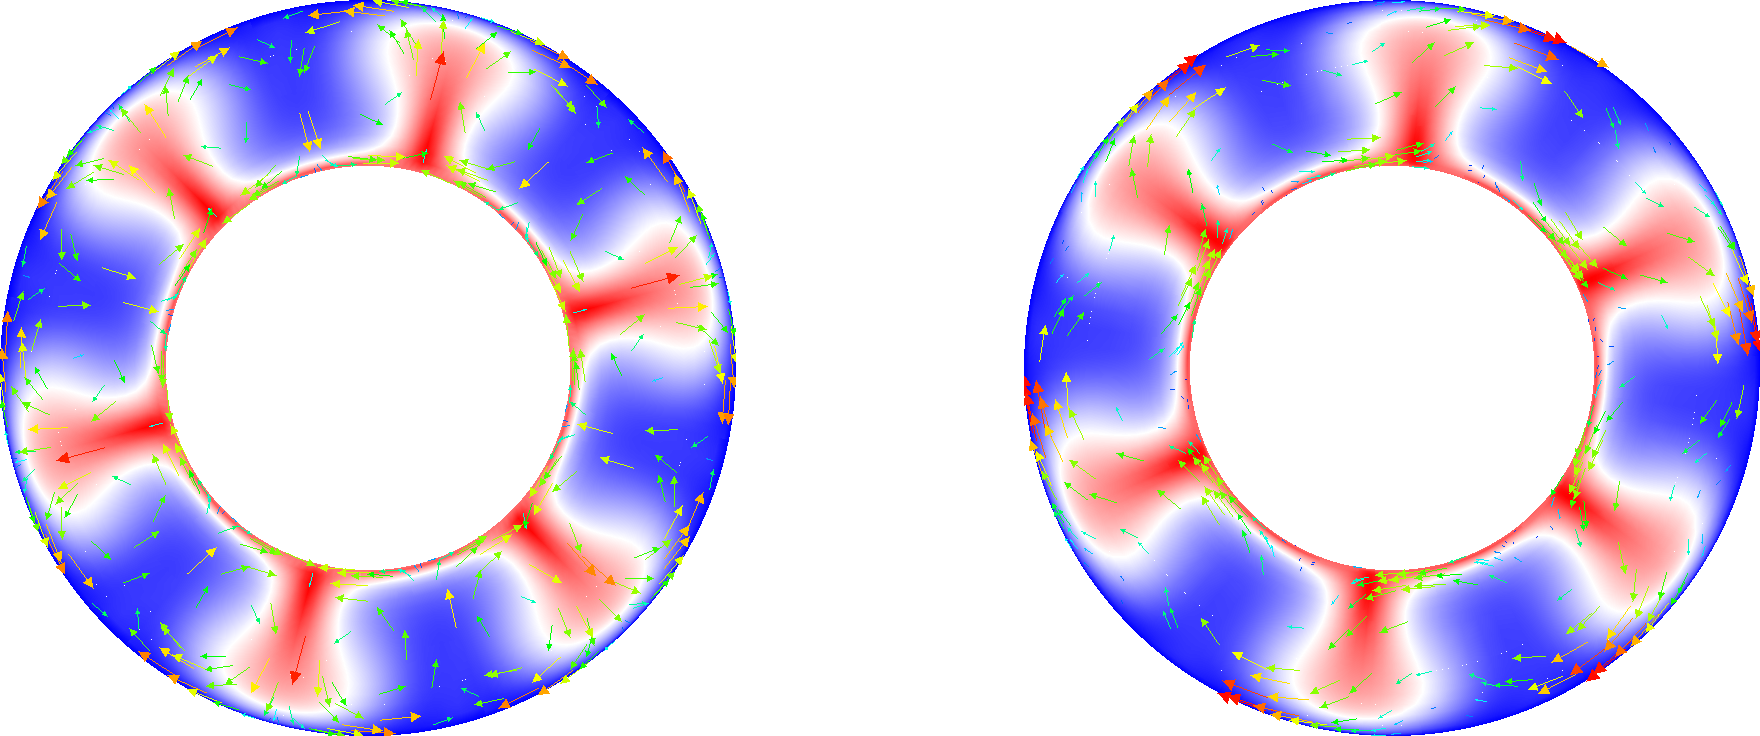
\includegraphics[width=0.8\textwidth]{rigid_rotation.png}
  \caption{\it Example of nullspace removal.
On the left the nullspace (a rigid rotation) is removed, and the velocity vectors accurately
show the mantle flow. On the right there is a significant clockwise rotation to the velocity
solution which is making the more interesting flow features difficult to see. }
  \label{fig:rigid_rotation}
\end{figure}


\subsection{Particles}
\label{sec:particles}

\aspect{} can, optionally, also deal with particles (sometimes called
``tracers''). Particles can be thought of as point-like objects that are simply
advected along with the flow. In other words, if $\mathbf u(\mathbf x,t)$ is the
flow field that results from solving equations
\eqref{eq:stokes-1}--\eqref{eq:stokes-2}, then the $k$th particle's position
satisfies the equations
\begin{align}
  \frac{d}{dt} \mathbf x_k(t)
  = \mathbf u(\mathbf x_k(t),t).
\end{align}
The initial positions of all particles also need to be given and are usually
either chosen randomly, based on a fixed pattern, or are read from a file.

Particles are typically used to track visually where material that starts
somewhere ends up after some time of a simulation. It can also be used to track
the \textit{history} of the volume of the fluid that surrounds a particle, for
example by tracking how much strain has accumulated, or what the minimal or maximal
temperature may have been in the medium along the trajectory of a particle. To
this end, particles can carry \textit{properties}. These are scalar-
or vector-valued quantities that are attached to each particle, that are
initialized at the beginning of a simulation, and that are then updated at each time step. In other words, if we
denote by $\mathbf p_{k,m}(t)$ the value of the $m$th property attached to
the $k$th particle, then $\mathbf p_{k,m}(t)$ will satisfy a differential
equation of the form
\begin{align*}
  \frac{\partial}{\partial t} \mathbf p_{k,m}(t)
  = \mathbf g_m\left(\mathbf p_{k,m},
  p(\mathbf x_k(t),t)), T(\mathbf x_k(t),t)),
  \varepsilon(\mathbf u(\mathbf x_k(t),t)),
  \mathfrak c(\mathbf x_k(t),t)\right).
\end{align*}
The exact form of $\mathbf g_m$ of course depends on what exactly a particular
property represents. Like with compositional fields (see
Section~\ref{sec:compositional}), it is possible to describe the right hand side
$\mathbf g_m$ in ways that also allows for impulse (delta) functions in time.

How particles are used in practice is probably best explained using examples. To
this end, see in particular Section~\ref{sec:cookbooks-particles}. All
particle-related input parameters are listed in
Section~\ref{parameters:Postprocess/Particles}. The implementation of particles is
discussed in great detail in \cite{gassmoeller_particles}.



\subsection{Geometric Multigrid}
\label{sec:gmg}

\aspect{} can optionally use a Geometric Multigrid Solver (GMG) for the efficient solution
of the Stokes system (velocity and pressure). When used correctly, this can
reduce the compute time spent in the solver by about a factor of 3,
and decrease the memory requirements by a factor of 10.
For more details
about the method see~\cite{clevenger_stokes19,clevenger_par_gmg}.

To take advantage of the GMG solver, you need to:
\begin{enumerate}
 \item Enable it in your parameter file, namely:
\lstinputlisting[language=prmfile]{cookbooks/overview/doc/gmg-enable.part.prm.out}
  See~\ref{parameters:Solver_20parameters/Stokes_20solver_20parameters} for other
  parameters that influence the solver behavior.

\item
  \index[prmindex]{Material averaging}
  \index[prmindexfull]{Material model!Material averaging}
  The GMG solver requires that the viscosity is averaged, either as a constant (for example by using harmonic averaging)
  or as a $Q_1$ averaging. (See Section~\ref{sec:sinker-with-averaging}
  for more about averaging.) Averaging other properties is optional. You can
  use
\lstinputlisting[language=prmfile]{cookbooks/overview/doc/gmg-average.part.prm.out}
for example. Note that $Q_1$ averaging is a bit slower than averaging to a constant per cell, but it
might provide more accurate solutions.

\item Run in release mode. The GMG solver depends on running optimized code, so using optimized mode
is more important than for other parts of ASPECT to get good
performance. (Of course, the GMG solver also runs in debug mode, and
you should do so while setting up a model. You will just not get the
same speedup from the non-GMG to the GMG solver in debug mode as you
get in release mode.)

\item Enable vectorization optimizations. The GMG solver takes advantage of special instructions (AVX2, AVX512)
in modern CPUs and requires these do be enabled when compiling \dealii{}. This can be achieved by passing the
compiler flag \texttt{CMAKE\_CXX\_FLAGS='-march=native'} to CMake or setting \texttt{NATIVE\_OPTIMIZATIONS=true} in \texttt{candi.cfg} when using candi (see~\ref{sec:installation} for more information).
When you have vectorization enabled, ASPECT will report something like
this:
\begin{lstlisting}[frame=single,language=ksh]
-----------------------------------------------------------------------------
-- This is ASPECT, the Advanced Solver for Problems in Earth's ConvecTion.
--     . version 2.3.0-pre
--     . using deal.II 9.2.0
--     .       with 64 bit indices and vectorization level 3 (512 bits)
--     . using Trilinos 12.10.1
--     . using p4est 2.2.0
--     . running in OPTIMIZED mode
--     . running with 114688 MPI processes
-----------------------------------------------------------------------------

Vectorization over 8 doubles = 512 bits (AVX512), VECTORIZATION_LEVEL=3
\end{lstlisting}
Without optimizations enabled, the output will be ``and vectorization
level 1 (128 bits)'' in the fourth line above.
\end{enumerate}




\section{Installation}
\label{sec:installation}

There are three distinct ways to install ASPECT -- compilation
from source, installing a virtual machine, and using a Docker container --
each providing distinct advantages and disadvantages. In this section we
describe all three options and start with a summary of their properties to
guide users to an informed decision about the best option for their purpose.

\begin{table}[htb]
  \center
  \begin{tabular}{|c|ccc|}
    \hline
    Feature & Compile \& Install & Virtual Machine & Docker Container \\
    \hline
    Speed overhead          & 0\%   & 30\%     & 0--5\%    \\
    Disk overhead           & 0~GB  & 1~GB     & 200~MB       \\
    Knowledge required      & Much  & Very Little & Little    \\
    Root privileges required & No   & No (installed VM software) & Partially  \\
    Embedded in native environment & Yes & No  & Partially    \\
    MacOS support           & Yes   & Yes      & Yes    \\
    Windows support         & No    & Yes      & Yes    \\
    Local parallelization   & Yes   & Yes      & Yes            \\
    Massively parallel computations & Yes & No & No \\
    Modifying ASPECT        & Possible & Possible & Possible \\
    Configuring dependencies & Possible & No   & No \\ \hline
  \end{tabular}
  \caption{\it Features of the different installation options of \aspect{}.}
  \label{tab:install-options}
\end{table}

The available options can be best presented in form of typical use cases:

\begin{enumerate}
\item Virtual Machine (\aspect{} beginner and tutorial participant): The
virtual machine image provides a fully prepared user environment that contains
installations of \aspect{}, all required libraries, and visualization software
on top of a full Linux environment. This way beginning users and tutorial
participants can work in a unified  environment, thus minimizing installation
time and technical problems. Due to the overhead of virtualizing a full
operating system this installation typically needs more space, and is
approximately 30~\% slower than a native installation. Additionally working in a
virtual machine `feels' differently from working in your usual desktop
environment. The virtual machine can be run on all host operating systems that
can run a virtualization software like VirtualBox (e.g. Linux, Apple MacOS,
Microsoft Windows).

\item Docker Container (advanced user with no need to configure/change the
underlying libraries, possibly changing parts of \aspect): Docker containers are
lightweight packages that only encapsulate the minimal dependencies to run an
application like \aspect{} on top of the host operating system. They allow easy
installation and usage of \aspect{} in a unified environment, while relying on
the user's operating system to provide visualization software and model input
data. When compared to the virtual machine it is simple to exchange files
between the host operating system and the docker container, and it provides the
benefit to work in the desktop environment you are used to. They have very
little overhead in terms of memory and speed compared to virtual machines, and
allow for reproducible computations. The container is set up with a standard
\aspect{} installation, but this can be modified by advanced users (source code
development within the container is possible).

\item Compile \& Install (advanced users and developers with the need to
reconfigure underlying libraries or running massively parallel models): The most
advanced option is to compile and install \aspect{} from source. This allows
maximal control over the underlying libraries like \trilinos{} and \dealii{}, as
well as easy modifications to \aspect{} by recompiling a modified source
directory. Our installation instructions cover most Linux and MacOS operating
systems, but incompatibilities on individual systems can always occur and make
the installation more cumbersome. If you are planning to run massively parallel
computations on a compute cluster this is likely your only option. Since
clusters usually have a very individual setup, it is always a good idea to ask
IT support staff for help when installing \aspect{}, to avoid hard to reproduce
setup problems, and performance penalties.
\end{enumerate}

\subsection{Docker Container}
\label{subsec:docker_container}

\subsubsection{Installing Docker and downloading the \aspect{} image}

Docker is a lightweight virtualization software that allows to ship
applications with all their dependencies in a simple way. It is outside of the
scope of this manual to explain all possible applications of Docker, and we
refer to the introduction (\url{https://www.docker.com/what-docker}) and
installation and quickstart guides
(\url{https://www.docker.com/products/docker}) on the Docker website for more
detailed descriptions of how to set up and use the docker engine. More
importantly Docker provides a marketplace for exchanging prepared docker images
(called Docker Hub). After setting up the docker engine downloading a
precompiled \aspect{} image from Docker Hub is as simple as typing in a
terminal:

\begin{lstlisting}[frame=single,language=ksh]
docker pull geodynamics/aspect
\end{lstlisting}

Note that the transfer size of the compressed image containing \aspect{} and
all its dependencies is about 900~MB. When extracted the image requires about
3.2~GB of disk space.

\subsubsection{Running \aspect{} models}
Although it is possible to use the downloaded \aspect{} docker image in a
number of different ways, we recommend the following workflow:

\begin{enumerate}
\item Create your \aspect{} input file in a folder of your choice (possibly
also containing any input data that is required by your model) and navigate in a
terminal into that directory.
\item Run the docker image and mount the current directory as a read-only
volume into the docker container\footnote{Note that it is possible to mount a
directory as writeable into the container. However, this is often associated
with file permission conflicts between the host system and the container.
Therefore, we recommend this slightly more cumbersome, but also more reliable
workflow.}. This is accomplished by specifying the -v flag followed by
the absolute path on the host machine, colon, absolute path within the docker
container, colon, and specifying read-only permissions as in the example below.

Make sure your parameter file specifies a model output directory \textit{other}
than the input directory, e.g. \texttt{/home/dealii/aspect/model\_output}. When
you have started the container run the aspect model inside the container. Note
that there are two \aspect{} executables in the work directory of the container:
\texttt{aspect} and \texttt{aspect-release}. For a discussion of the
different versions see Section~\ref{sec:debug-mode}, in essence: You should run
\texttt{aspect} first to check your model for errors, then run
\texttt{aspect-release} for a faster model run.

To sum up, the steps you will want to execute are:
\begin{lstlisting}[frame=single,language=ksh,showstringspaces=false]
docker run -it -v "$(pwd):/home/dealii/aspect/model_input:ro" \
  geodynamics/aspect:latest bash
\end{lstlisting}

Within the container, simply run your model by executing:

\begin{lstlisting}[frame=single,language=ksh]
./aspect model_input/your_input_file.prm
\end{lstlisting}

\item After the model has finished (or during the model run if you want to check
intermediate results) copy the model output out of the container into your
current directory. For this you need to find the name or ID of the docker
container by running \texttt{docker ps -a} in a separate terminal first. Look
for the most recently started container to identify your current \aspect{}
container.

Commands that copy the model output to the current directory could be:
\begin{lstlisting}[frame=single,language=ksh]
docker ps -a # Find the name of the running / recently closed container in the output
docker cp CONTAINER_NAME:/home/dealii/aspect/model_output .
\end{lstlisting}

\item The output data is saved inside your container even after the computation
finishes and even when you stop the container. After you have copied the data
out of the container you should therefore delete the container to avoid
duplication of output data. Even after deleting you will always be able to start
a new container from the downloaded image following step 2. Deleting the
finished container can be achieved by the \texttt{docker container prune}
command that removes any container that is not longer running.
\note{If you own other finished containers that you want to keep use
\texttt{docker container rm CONTAINER\_NAME} to only remove the container named
\texttt{CONTAINER\_NAME}.}

To remove all finished containers use the following command:
\begin{lstlisting}[frame=single,language=ksh]
docker container prune
\end{lstlisting}
Alternatively only remove a particular container:
\begin{lstlisting}[frame=single,language=ksh]
docker container rm CONTAINER_NAME
\end{lstlisting}
\end{enumerate}

You are all set. Repeat steps 1-4 of this process as necessary when updating
your model parameters.

\subsubsection{Developing \aspect{} within a container}

The above given workflow does not include advice on how to modify \aspect{}
inside the container. We recommend a slightly different workflow for advanced
users that want to modify parts of \aspect{}. The \aspect{} docker container
itself is build on top of a \dealii{} container that contains all dependencies
for compiling \aspect{}. Therefore it is possible to run the deal.II container,
mount an \aspect{} source directory from your host system and compile it inside
of the container. An example workflow could look as following (assuming you
navigated in a terminal into the modified \aspect{} source folder):

\begin{lstlisting}[frame=single,language=ksh,showstringspaces=false]
docker pull geodynamics/aspect:latest
docker run -it -v "$(pwd):/home/dealii/aspect:ro" geodynamics/aspect:latest
\end{lstlisting}

Inside of the container you now find a read-only \aspect{} directory that
contains your modified source code. You can compile and run a model inside the
container, e.g. in the following way:

\begin{lstlisting}[frame=single,language=ksh]
mkdir aspect-build
cd aspect-build
cmake -DCMAKE_BUILD_TYPE=Debug $HOME/aspect
make -j4
./aspect $HOME/aspect/cookbooks/shell_simple_2d/shell_simple_2d.prm
\end{lstlisting}

To avoid repeated recompilations of the \aspect{} source folder we recommend to
reuse the so prepared container instead of starting new containers based on the
\dealii{} image. This can be achieved by the following commands outside of the
container:

\begin{lstlisting}[frame=single,language=ksh]
docker ps -a # Find the name of the running / recently closed container in the output
docker restart CONTAINER_NAME
docker attach CONTAINER_NAME
\end{lstlisting}

For more information on the differences between using images and containers,
and how to attach additional terminals to a running container, we refer to the
docker documentation (e.g.
\url{https://docs.docker.com/engine/getstarted/step_two/}).

\subsection{Virtual Machine}

\subsubsection{Installing VM software and setting up the virtual machine}

The \aspect{} project provides an experimental virtual machine containing a
fully configured version of \aspect{}. To use this machine, you will need to
install VirtualBox (\url{http://www.virtualbox.org/}) on your machine, and then
import a virtual machine image that can be downloaded from
\url{http://www.math.clemson.edu/~heister/dealvm/}. Note, however, that the
machine image is several gigabytes in size and downloading will take a while.
After downloading and installing the virtual image it is convenient to set up a
shared folder between your host system and the virtual machine to exchange model
files and outputs.

\subsubsection{Running \aspect{} models}

The internal setup of the virtual machine is similar to the Docker container
discussed above, except that it contains a full-featured desktop environment.
Also note that the user name is \texttt{ubuntu}, not \texttt{dealii} as in the
Docker container. Again there are multiple ways to use the virtual machine, but
we recommend the following workflow:

\begin{enumerate}
\item Create your \aspect{} input file in the shared folder and start the
virtual machine.
\item Navigate in a terminal to your model directory.
\item Run your model using the provided \aspect{} executable:

\begin{lstlisting}[frame=single,language=ksh]
~/aspect/aspect your_input_file.prm
\end{lstlisting}

\item The model output should automatically appear on your host machine in the
shared directory.

\item After you have verified that your model setup is correct, you might want
to consider recompiling \aspect{} in release mode to increase the speed of the
computation. See Section~\ref{sec:debug-mode} for a discussion of debug and
release mode.

\item Visualize your model output either inside of the virtual machine
(ParaView and VisIt are pre-installed), or outside on your host system.
\end{enumerate}

You are all set. Repeat steps 1-6 of this process as necessary when updating
your model parameters.

\subsection{Local installation}

This is a brief explanation of how to compile and install the required dependencies and
\aspect{} itself. This installation procedure guarantees fastest runtimes, and largest flexibility,
but usually requires more work than the options mentioned in the previous sections.
While it is possible to install ASPECT's dependencies in particular \pfrst{}, \trilinos{},
and \dealii{} manually, we recommend to use the
\texttt{candi} software (see \url{https://github.com/dealii/candi}). \texttt{candi} was written
as an installation program for deal.II, and includes a number of system specific instructions
that will be listed when starting the program. It can be flexibly configured to allow for
non-default compilers or libraries (e.g. Intel's MKL instead of LAPACK) by changing entries
in the configuration file \texttt{candi.cfg}, or by providing platform specific installation files.

In case you encounter problems during the installation, please consult our wiki
(\url{https://github.com/geodynamics/aspect/wiki}) for frequently asked
questions and special instructions for MacOS users, before posting your
questions on the forum (\url{https://community.geodynamics.org/c/aspect}).

\subsubsection{System prerequisites}

\texttt{candi} will show system specific instructions on startup, but its prerequisites
are relatively widely used and packaged
for most operating systems. You will need compilers for C, C++ and
Fortran, the GNU make system, the CMake build system, and the libraries and
header files of BLAS, LAPACK and zlib, which is used for compressing
the output data. To use more than one process for your computations
you will need to install a MPI library, its headers and the
necessary executables to run MPI programs. There are some optional packages
for additional features, like the HDF5 libraries for additional output formats
 and Numdiff for checking \aspect{}'s test
results with reasonable accuracy, but these are not strictly required, and in
some operating systems they are not available as packages but need to be
compiled from scratch.
Finally, for obtaining a recent development version of \aspect{} you will
need the git version control system.

An exemplary command to obtain all required packages on Ubuntu 14.04 would be:
\begin{verbatim}
sudo apt-get install build-essential \
                     cmake \
                     gcc \
                     g++ \
                     gfortran \
                     git \
                     libblas-dev \
                     liblapack-dev \
                     libopenmpi-dev \
                     numdiff \
                     openmpi-bin \
                     zlib1g-dev
\end{verbatim}

\subsubsection{Using candi to compile dependencies}

In its default configuration \texttt{candi} downloads and
compiles a \dealii{} configuration that is able to run \aspect, but it
also contains a number of packages that are not required (and that can
be safely disabled if problems occur during the
installation). We require at least the packages \pfrst{}, \trilinos{},
and finally \dealii{}.

At the time of this writing \texttt{candi} will install \pfrst{} 2.2,
\trilinos{} 12.18.1, and \dealii{} 9.3.0.
We strive to keep the development version of \aspect{} compatible with
the latest release of \dealii{} and the current \dealii{} development
version at any time, and we usually support several older versions of
\pfrst{} and \trilinos{}.

\begin{enumerate}
\item \textit{Obtaining candi:} Download \texttt{candi} by running
    \begin{verbatim}
    git clone https://github.com/dealii/candi
    \end{verbatim}
    in a directory of your choice.

\item \textit{Installing \dealii{} and its dependencies:} Execute \texttt {candi} by running
    \begin{verbatim}
    cd candi
    ./candi.sh -p INSTALL_PATH
    \end{verbatim}
    (here we assume you replace \texttt{INSTALL\_PATH} by the path were
    you want to install all dependencies and \dealii{}, typically a directory inside
    \texttt{\$HOME/bin} or a similar place).
    This step might take a long time, but can be parallelized by adding
    \texttt{-jN}, where
    \texttt{N} is the number of CPU cores available on your computer. Further configuration options
    and parameters are listed at \url{https://github.com/dealii/candi}. In case you encounter
    problems during this step, please read the error message, and consult our wiki
    (\url{https://github.com/geodynamics/aspect/wiki}) for common installation problems,
    before asking on the forum (\url{https://community.geodynamics.org/c/aspect}).

\item You may now want to configure your environment to make it aware of the newly installed
    packages. This can be achieved by adding the line
    \texttt{source INSTALL\_PATH/configuration/enable.sh} to the file responsible for setting
    up your shell environment\footnote{For bash this would be the file \texttt{\~{}/.bashrc}.}
    (again we assume you replace \texttt{INSTALL\_PATH} by the patch chosen in the previous step).
    Then close the terminal and open it again to activate the change.

\item \textit{Testing your installation:} Test that your installation works
  by compiling the {\texttt{step-32}} example that you can find in
  {\texttt{\$DEAL\_II\_DIR/examples/step-32}}. Prepare and compile by running {\texttt{cmake . \&\& make}}
  and run with {\texttt{mpirun -n 2 ./step-32}}.

\end{enumerate}

Congratulations, you are now set up for compiling \aspect{} itself.

\subsubsection{Obtaining \aspect{} and initial configuration}

The development version of \aspect{} can be downloaded by executing the command
\begin{verbatim}
 git clone https://github.com/geodynamics/aspect.git
\end{verbatim}
If {\texttt{\$DEAL\_II\_DIR}} points to your \dealii{} installation, you can configure
\aspect{} by running
\begin{verbatim}
 mkdir build; cd build; cmake ..
\end{verbatim}
in the \aspect{} directory created by the {\texttt{git clone}} command above.
If you did not set {\texttt{\$DEAL\_II\_DIR}} you have to supply cmake with the location:
\begin{verbatim}
 cmake -DDEAL_II_DIR=/u/username/deal-installed/ ..
\end{verbatim}

This will create an ``out-of-source`` build, where the build directory is
different from the source directory. While in-source builds (where you run
\texttt{cmake .} in your source directory), are supported, we strongly
recommend an out-of-source build as described above. Specifically, running
the whole test suite (see Section~\ref{sec:running_tests}) is only supported
this way.

\subsubsection{Compiling \aspect{} and generating documentation}
\label{sec:compiling}

After downloading \aspect{} and having built the libraries it builds on, you
can compile it by typing
\begin{verbatim}
  make
\end{verbatim}
on the command line (or \texttt{make -jN} if you have multiple processors in
your machine, where \texttt{N} is the number of processors). This builds the
\aspect{} executable which will reside in the \texttt{build} directory
and will be named \texttt{aspect}. To run \aspect{} from the main source directory
you would need to reference it as \texttt{./build/aspect}.
If you intend to
modify \aspect{} for your own experiments, you may want to also generate
documentation about the source code. This can be done using the command
\begin{verbatim}
  cd doc; make
\end{verbatim}
which assumes that you have the \texttt{doxygen} documentation generation tool
installed. Most Linux distributions have packages for \texttt{doxygen}. The
result will be the file \url{doc/doxygen/index.html} that is the starting
point for exploring the documentation.


%%%%%%%%%%%%%%%%%%%%%%

\section{Running \aspect}
\label{sec:running}

\subsection{First steps}
\label{sec:first-steps}
Before trying to set up a model to answer your particular research questions,
we advise you to get familiar with \aspect{} and its functionalities by
following these steps:
\begin{enumerate}
\item Watch the CIG \aspect{} tutorials (\url{https://www.youtube.com/playlist?list=PLdy04DoEepEyeS_HZwa0Ws0kW5Rs2wsQ6})
that will show you how to run \aspect{} and construct new setups yourself.
\item Go through the cookbooks in this manual, see Section~\ref{sec:cookbooks}.
\item Go through the benchmarks in this manual, see Section~\ref{sec:cookbooks-benchmarks}.
\item If you want to use some existing functionality that is not discussed in these resources,
search in the extensive tests directory. For example, to search for an initial temperature condition called
``spherical gaussian perturbation'' while in the \aspect{} directory, type:
\begin{verbatim}
  grep 'spherical gaussian perturbation' tests/*.prm
\end{verbatim}
This command will show you all the test input files that use this initial temperature condition.
You can also look up any of the parameters used in the input files in this manual.
\item Have a look at the \aspect{} GitHub repository. Here you can see the planned developments
(\url{https://github.com/geodynamics/aspect/projects/2}), current issues that others have reported
(\url{https://github.com/geodynamics/aspect/issues}), and what is currently being worked on
(\url{https://github.com/geodynamics/aspect/pulls}).
\item Have a look at our discussion forum when your model behaves unexpectedly
or you need functionality that does not exist yet. The \aspect{} community can tell you
whether they experienced something similar or are already working on the topic.
\item If you experience unexpected behavior that you expect is a bug and this problem
has not been reported as an issue on GitHub, please create a new issue so that everybody
is aware of the potential problem and can think of a fix. When creating a new issue,
it is very useful if you can provide a minimum working example, i.e. a small test setup
that demonstrates the issue and does not require modifications to the code. You can for example
modify one of the existing test input files, which typically take less than a minute to
run using only a few cores.
The test input file and an image illustrating the problem can be attached to the issue.
\end{enumerate}

\subsection{Overview}
\label{sec:running-overview}

After compiling \aspect{} as described above, you should have an executable
file in the build directory. It can be called in the build directory as follows:
\begin{verbatim}
  ./aspect parameter-file.prm
\end{verbatim}
or, if you want to run the program in parallel, using something like
\begin{verbatim}
  mpirun -np 4 ./aspect parameter-file.prm
\end{verbatim}
to run with 4 processors. In either case, the argument denotes the (path and)
name of a file that contains input parameters.%
\footnote{As a special case, if you call \aspect{} with an argument that
consists of two dashes, ``\texttt{-{}-}'', then the arguments will be read from
the standard input stream of the program. In other words, you could type the
input parameters into your shell window in this case (though that would be
cumbersome, \aspect{} would seem to hang until you finish typing all of your
input into the window and then terminating the input stream by typing
\texttt{Ctrl-D}). A more common case would be to use Unix pipes so that the
default
input of \aspect{} is the output of another program, as in a command like
\texttt{cat parameter-file.prm.in | mypreprocessor | ./aspect -{}-}, where
\texttt{mypreprocessor} would be a program of your choice that somehow
transforms the file \texttt{parameter-file.prm.in} into a valid input file,
for example to systematically vary one of the input parameters.

If you want to run \aspect{} in parallel, you can do something like
\texttt{cat parameter-file.prm.in | mypreprocessor | mpirun -np 4 ./aspect
  -{}-}. In cases like this, \texttt{mpirun} only forwards the output of
\texttt{mypreprocessor} to the first of the four MPI processes, which then
sends the text to all other processors.}
When you download \aspect{}, there are a number of sample input files in the
\texttt{cookbooks} directory, corresponding to the examples discussed in
Section~\ref{sec:cookbooks}, and input files for some of the benchmarks discussed
in Section~\ref{sec:cookbooks-benchmarks} are located in the \texttt{benchmarks}
directory. A full description of all parameters one can specify in these files
is given in Section~\ref{sec:parameters}.

Running \aspect{} with an input file
\footnote{For example by running \texttt{./aspect ../cookbooks/convection-box/convection-box.prm} in
your build directory.}
will produce output that will look
something like this (numbers will all be different, of course):
\begin{lstlisting}[frame=single,language=ksh]
-----------------------------------------------------------------------------
-- This is ASPECT, the Advanced Solver for Problems in Earth's ConvecTion.
--     . version 2.0.0-pre (include_dealii_version, c20eba0)
--     . using deal.II 9.0.0-pre (master, 952baa0)
--     . using Trilinos 12.10.1
--     . using p4est 2.0.0
--     . running in DEBUG mode
--     . running with 1 MPI process
-----------------------------------------------------------------------------

Number of active cells: 1,536 (on 5 levels)
Number of degrees of freedom: 20,756 (12,738+1,649+6,369)

*** Timestep 0:  t=0 years

   Rebuilding Stokes preconditioner...
   Solving Stokes system... 30+3 iterations.
   Solving temperature system... 8 iterations.

Number of active cells: 2,379 (on 6 levels)
Number of degrees of freedom: 33,859 (20,786+2,680+10,393)

*** Timestep 0:  t=0 years

   Rebuilding Stokes preconditioner...
   Solving Stokes system... 30+4 iterations.
   Solving temperature system... 8 iterations.

   Postprocessing:
     Writing graphical output: output/solution/solution-00000
     RMS, max velocity:        0.0946 cm/year, 0.183 cm/year
     Temperature min/avg/max:  300 K, 3007 K, 6300 K
     Inner/outer heat fluxes:  1.076e+05 W, 1.967e+05 W

*** Timestep 1:  t=1.99135e+07 years

   Solving Stokes system... 30+3 iterations.
   Solving temperature system... 8 iterations.

   Postprocessing:
     Writing graphical output: output/solution/solution-00001
     RMS, max velocity:        0.104 cm/year, 0.217 cm/year
     Temperature min/avg/max:  300 K, 3008 K, 6300 K
     Inner/outer heat fluxes:  1.079e+05 W, 1.988e+05 W

*** Timestep 2:  t=3.98271e+07 years

   Solving Stokes system... 30+3 iterations.
   Solving temperature system... 8 iterations.

   Postprocessing:
     RMS, max velocity:       0.111 cm/year, 0.231 cm/year
     Temperature min/avg/max: 300 K, 3008 K, 6300 K
     Inner/outer heat fluxes: 1.083e+05 W, 2.01e+05 W

*** Timestep 3:  t=5.97406e+07 years

...
\end{lstlisting}

The output starts with a header that lists the used \aspect{}, \dealii{},
\trilinos{} and \pfrst{} versions as well as the mode you compiled \aspect{} in
(see \ref{sec:debug-mode}), and the number of parallel processes
used\footnote{If you used the \texttt{git} version control system to download
\aspect{} and/or \dealii{}, as in this example, you will also get the current
branch, and unique revision identifier for the current version. This is very
important if you modify either software between releases, or you use a
development version that is not an official release. Note that this revision
can not track changes you made to the software that are not part of a git
commit.}.  With this information we strive to make
\aspect{} models as reproducible as possible.

The following output depends on the model, and in this case was produced by
a parameter file that, among other settings, contained the following values
(we will discuss many such input files in Section~\ref{sec:cookbooks}:
\lstinputlisting[language=prmfile]{cookbooks/overview/doc/simple.prm.out}

In other words, these run-time parameters specify that we should start with a
geometry that represents a spherical shell (see
Sections~\ref{parameters:Geometry_20model} and
\ref{parameters:Geometry_20model/Spherical_20shell} for details). The coarsest
mesh is refined 4 times globally, i.e., every cell is refined into four
children (or eight, in 3d) 4 times. This yields the initial number of 1,536
cells on a mesh hierarchy that is 5 levels deep. We then solve the problem
there once and, based on the number of adaptive refinement steps at the
initial time set in the parameter file, use the solution so computed to refine
the mesh once adaptively (yielding 2,379 cells on 6 levels) on which we start
the computation over at time $t=0$.

Within each time step, the output indicates the number of iterations performed
by the linear solvers, and we generate a number of lines of output by the
postprocessors that were selected (see
\index[prmindex]{List of postprocessors}
\index[prmindexfull]{Postprocess!List of postprocessors}
Section~\ref{parameters:Postprocess}). Here, we have selected to run all
postprocessors that are currently implemented in \aspect{} which includes the
ones that evaluate properties of the velocity, temperature, and heat flux as
well as a postprocessor that generates graphical output for visualization.

While the screen output is useful to monitor the progress of a simulation,
its lack of a structured output makes it not useful for later plotting things
like the evolution of heat flux through the core-mantle boundary. To this end,
\aspect{} creates additional files in the output directory selected in the
input parameter file
\index[prmindex]{Output directory}
\index[prmindexfull]{Output directory}
(here, the \texttt{output/} directory relative to the
directory in which \aspect{} runs). In a simple case, this will look as
follows:
\begin{lstlisting}[frame=single,language=ksh]
aspect> ls -l output/
total 932
-rw-rw-r-- 1 bangerth bangerth  11134 Dec 11 10:08 depth_average.gnuplot
-rw-rw-r-- 1 bangerth bangerth  11294 Dec 11 10:08 log.txt
-rw-rw-r-- 1 bangerth bangerth     42 Dec 11 10:07 original.prm
-rw-rw-r-- 1 bangerth bangerth 326074 Dec 11 10:07 parameters.prm
-rw-rw-r-- 1 bangerth bangerth 577138 Dec 11 10:07 parameters.tex
drwxr-xr-x 2 bangerth bangerth   4096 Dec 11 10:08 solution
-rw-rw-r-- 1 bangerth bangerth    484 Dec 11 10:08 solution.pvd
-rw-rw-r-- 1 bangerth bangerth    451 Dec 11 10:08 solution.visit
-rw-rw-r-- 1 bangerth bangerth   8267 Dec 11 10:08 statistics
\end{lstlisting}
The purpose of these files is as follows:
\begin{itemize}

\item \textit{Screen output:} The file \texttt{output/log.txt} contains a copy
  of the output that is printed to the terminal when you run \aspect{}.

\item \textit{A listing of all run-time parameters:} The file
  \texttt{output/original.prm} is a copy of the parameter file that was used
  in this computation. It is often useful to save this file together with
  simulation data to allow for the easy reproduction of computations later on.

  The \texttt{output/parameters.prm} file contains a complete listing of all
  run-time parameters. In particular, this includes the ones that have been
  specified in the input parameter file passed on the command line, but it
  also includes those parameters for which defaults have been used. This file
  can also be used to explore all available parameters and possible options as
  it contains the documentation of all parameters.

  Finally, there is \texttt{output/parameters.tex}, that lists the parameters
  like \texttt{output/parameters.prm} in \LaTeX{} format, and
  \texttt{output/parameters.json} in JSON format.

  While \texttt{output/parameters.prm} contains all parameters (with their
  default values if they were not specified), all formatting and comments are
  lost. As \texttt{output/original.prm} is identical to the prm you started
  \aspect{} with, it preserves comments and formatting while not outputting
  the default values (or documentation).

\item \textit{Graphical output files:} One of the postprocessors chosen
  in the parameter file used for this computation is the one that generates
  output files that represent the solution at certain time steps. The screen output
  indicates that it has run at time step 0, producing output files that start
  with \texttt{output/solution/solution-00000}. Depending on the settings in the
  parameter file, output will be generated every so many seconds or years of
  simulation time, and subsequent output files will then start with
  \texttt{output/solution/solution-00001}, all placed in the
  \texttt{output/solution} subdirectory. This is because there are often
  \textit{a lot} of output files: For many time steps, times the number of
  processors, so they are placed in a subdirectory so as not to make it more
  difficult than necessary to find the other files.

  At the current time, the
  default is that \aspect{} generates this output in VTK format%
  \footnote{The output is in fact in the VTU version of the VTK file
    format. This is the XML-based version of this file format in which
    contents are compressed. Given that typical file sizes for 3d simulation
    are substantial, the compression saves a significant amount of disk
    space.}  as that is widely used by a number of excellent visualization
  packages and also supports parallel visualization.%
  \footnote{The underlying \dealii{} package actually supports output in
    around a dozen different formats, but most of them are not very useful for
    large-scale, 3d, parallel simulations. If you need a different format than
    VTK, you can select this using the run-time parameters discussed in
    Section~\ref{parameters:Postprocess/Visualization}.}  If
  the program has been run with multiple MPI processes, then the list of
  output files will be \texttt{output/solution/solution-XXXXX.YYYY}
  denoting that this the \texttt{XXXXX}th time we create output files and that
  the file was generated by the \texttt{YYYY}th processor.

  VTK files can be visualized by many of the large visualization packages. In
  particular, the
  \href{https://visit.llnl.gov}{Visit} and
  \href{http://www.paraview.org/}{ParaView} programs, both
  widely used, can read the files so created. However, while VTK has become a
  de-facto standard for data visualization in scientific computing, there
  doesn't appear to be an agreed upon way to describe which files jointly make
  up for the simulation data of a single time step (i.e., all files with the
  same \texttt{XXXXX} but different \texttt{YYYY} in the example above). Visit
  and ParaView both have their method of doing things, through \texttt{.pvtu} and
  \texttt{.visit} files. To make it easy for you to view data, \aspect{}
  simply creates both kinds of files in each time step in which graphical data
  is produced, and these are then also placed into the subdirectories as
  \texttt{output/solution/solution-XXXXX.pvtu} and
  \texttt{output/solution/solution-XXXXX.visit}.

  The final two files of this kind, \texttt{output/solution.pvd} and
  \texttt{output/solution.visit}, are files that
  describes to ParaView and Visit, respectively, which
  \texttt{output/solution/solution-XXXXX.pvtu} and
  \texttt{output/solution/solution-XXXXX.YYYY.vtu} jointly form a complete
  simulation.
  In the former case, the file lists the \texttt{.pvtu} files of all
  timesteps together with the simulation time to which they correspond. In the
  latter case, it actually lists all \texttt{.vtu} that belong to one
  simulation, grouped by the timestep they correspond to.
  To visualize an entire simulation, not just a single time step, it is
  therefore simplest to just load one of these files, depending on whether you
  use ParaView or Visit.%
  \footnote{At the time of writing this, current versions of Visit (starting
    with version 2.5.1) actually have a bug that prevents them from
    successfully reading the \texttt{output/solution.visit} or
    \texttt{output/solution/solution-XXXXX.visit} files -- Visit believes that
    each of these files corresponds to an individual time step, rather than that a whole
    group of files together form one time step. This bug is not fixed in Visit
    2.6.3, but may be fixed in later versions.}
  Because loading an \textit{entire} simulation is the most common use case,
  these are the two files you will most often load, and so they are placed in
  the \texttt{output} directory, not the subdirectory where the actual
  \texttt{.vtu} data files are located.

  For more on visualization, see also Section~\ref{sec:viz}.

\item \textit{A statistics file:} The \texttt{output/statistics} file contains
  statistics collected during each time step, both from within the simulator
  (e.g., the current time for a time step, the time step length, etc.) as well
  as from the postprocessors that run at the end of each time step. The file
  is essentially a table that allows for the simple production of time
  trends. In the example above, and at the time when we are writing this
  section, it looks like this:
  \begin{lstlisting}[frame=single,language=ksh,showstringspaces=false]
# 1: Time step number
# 2: Time (years)
# 3: Iterations for Stokes solver
# 4: Time step size (year)
# 5: Iterations for temperature solver
# 6: Visualization file name
# 7: RMS velocity (m/year)
# 8: Max. velocity (m/year)
# 9: Minimal temperature (K)
# 10: Average temperature (K)
# 11: Maximal temperature (K)
# 12: Average nondimensional temperature (K)
# 13: Core-mantle heat flux (W)
# 14: Surface heat flux (W)
0 0.000e+00 33 2.9543e+07 8                             "" 0.0000 0.0000 0.0000 0.0000    ...
0 0.000e+00 34 1.9914e+07 8 output/solution/solution-00000 0.0946 0.1829 300.00 3007.2519 ...
1 1.991e+07 33 1.9914e+07 8 output/solution/solution-00001 0.1040 0.2172 300.00 3007.8406 ...
2 3.982e+07 33 1.9914e+07 8                             "" 0.1114 0.2306 300.00 3008.3939 ...
  \end{lstlisting}
  The actual columns you have in your statistics file may differ from the ones above,
  but the format of this file should be obvious. Since the hash mark is a comment
  marker in many programs (for example, \texttt{gnuplot} ignores lines in text
  files that start with a hash mark), it is simple to plot these columns as time
  series. Alternatively, the data can be imported into a spreadsheet and
  plotted there.
\note{As noted in Section~\ref{sec:non-dimensional}, \aspect{} can be
  thought of as using the meter-kilogram-second (MKS, or SI) system. Unless otherwise noted,
  the quantities in the output file are therefore also in MKS units.}

  A simple way to plot the contents of this file is shown in Section~\ref{sec:viz-stat}.

\item \textit{Output files generated by other postprocessors:} Similar to the
  \texttt{output/statistics} file, several of the existing
  postprocessors one can select from the parameter file generate their
  data in their own files in the output directory. For example, \aspect{}'s
  ``depth average'' postprocessor will write depth-average statistics into
  the file \texttt{output/depth\_average.gnuplot}.
  Input parameters chosen in the input file control how often this file is
  updated by the postprocessor, as well as what graphical file format to use (if
  anything other than \texttt{gnuplot} is desired).

  By default, the data is written in text format that can be easily visualized,
  see for example Figure~\ref{fig:depthaverage}. The plot
  shows how an initially linear temperature profile forms upper and lower
  boundary layers.

\begin{figure}[tbp]
  \centering
  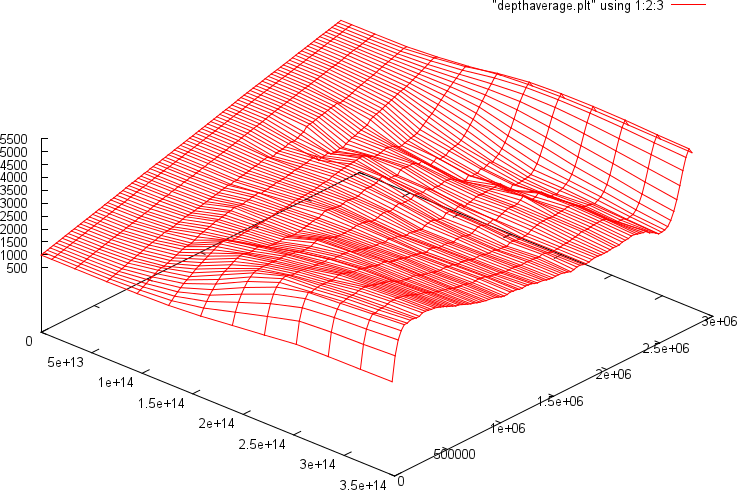
\includegraphics[width=0.6\textwidth]{depthaverage2.png}
  \caption{\it Example output for depth average statistics. On the left axis are 13 time
  steps, on the right is the depth (from the top at 0 to the bottom of the mantle on the
  far right), and the upwards pointing axis is the average temperature. This
  plot is generated by gnuplot, but the depth averages can be written in many
  other output formats as well, if preferred (see
  Section~\ref{parameters:Postprocess/Depth_20average}).}
  \label{fig:depthaverage}
\end{figure}

\end{itemize}

There are other parts of \aspect{} that may also create files in the output
directory. For example, if your simulation includes advecting along particles
(see Section~\ref{sec:particles}), then visualization information for these
particles will also appear in this file. See
Section~\ref{sec:cookbooks-particles} for an example of how this looks like.


\subsection{Selecting between 2d and 3d runs}
\label{sec:2d-vs-3d}

\aspect{} can solve both two- and three-dimensional problems.%
\footnote{For a description of what exactly we mean when we consider
two-dimensional models, see Section~\ref{sec:meaning-of-2d}.}
You select which one you want by putting a line like the following into
\index[prmindex]{Dimension}
\index[prmindexfull]{Dimension}
the parameter file (see Section~\ref{sec:parameters}):
\lstinputlisting[language=prmfile]{cookbooks/overview/doc/dim.part.prm.out}

Internally, dealing with the dimension builds on a feature in
\dealii{}, upon which \aspect{} is based, that is called
\textit{dimension-independent programming}. In essence, what this does is that
you write your code only once in a way so that the space dimension is a
variable (or, in fact, a template parameter) and you can compile the code for
either 2d or 3d. The advantage is that codes can be tested and debugged in 2d
where simulations are relatively cheap, and the same code can then be
re-compiled and executed in 3d where simulations would otherwise be
prohibitively expensive for finding bugs; it is also a useful feature when
scoping out whether certain parameter settings will have the desired effect by
testing them in 2d first, before running them in 3d. This feature is discussed
in detail in the
\href{https://www.dealii.org/developer/doxygen/deal.II/step_4.html}{\dealii{}
  tutorial program step-4}.
Like there, all the functions and classes in
\aspect{} are compiled for both 2d and 3d. Which dimension is actually
called internally depends on what you have set in the input file, but
in either case, the machine code generated for 2d and 3d results from
the same source code and should, thus, contain the same set of
features and bugs. Running in 2d and 3d should therefore yield
comparable results. Be prepared to wait much longer for
computations to finish in the latter case, however.


\subsection{Debug or optimized mode}
\label{sec:debug-mode}

\aspect{} utilizes a \dealii{} feature called \textit{debug
  mode}. By default, \aspect{} uses debug mode, i.e., it calls a version of
the \dealii{} library that contain lots of checks for the correctness of
function arguments, the consistency of the internal state of data structure,
etc. If you program with \dealii{}, for example to extend \aspect{}, it has
been our experience over the years that, by number, most programming errors are of the
kind where one forgets to initialize a vector, one accesses data that has not
been updated, one tries to write into a vector that has ghost elements,
etc. If not caught, the result of these bugs is that parts of the program use
invalid data (data written into ghost elements is not communicated to other
processors), that operations simply make no sense (adding vectors of different
length), that memory is corrupted (writing past the end of an array) or, in
rare and fortunate cases, that the program simply crashes.

Debug mode is designed to catch most of these errors: It enables some 7,300
assertions (as of late 2011) in \dealii{} where we check for errors like the
above and, if the condition is violated, abort the program with a detailed
message that shows the failed check, the location in the source code, and a
stacktrace how the program got there. The downside of debug mode is, of
course, that it makes the program much slower -- depending on application by a
factor of 4--10. An example of the speedup one can get is shown in
Section~\ref{sec:cookbooks-simple-box}.

\aspect{} by default uses debug mode because most users will want to play with
the source code, and because it is also a way to verify that the compilation
process worked correctly. If you have verified that the program runs correctly
with your input parameters, for example by letting it run for the first 10
time steps, then you can switch to optimized mode by compiling \aspect{}
with the command\footnote{Note that this procedure also changed with the switch to cmake.}
\begin{verbatim}
 make release
\end{verbatim}
and then compile using
\begin{verbatim}
 make
\end{verbatim}
To switch back to debug mode type:
\begin{verbatim}
 make debug
\end{verbatim}

\note{It goes without saying that if you make significant modifications to the
  program, you should do the first runs in debug mode to verify that your
  program still works as expected.}


\subsection{Visualizing results}
\label{sec:viz}

Among the postprocessors that can be selected in the input parameter file (see
Sections~\ref{sec:running-overview} and
\ref{parameters:Postprocess/Visualization}) are some that can produce files in
a format that can later be used to generate a graphical visualization of the
solution variables $\mathbf u, p$ and $T$ at select time steps, or of
quantities derived from these variables (for the latter, see
Section~\ref{sec:viz-postpostprocessors}).

By default, the files that are generated are in VTU format, i.e., the
XML-based, compressed format defined by the VTK library, see
\url{http://public.kitware.com/VTK/}. This file format has become a broadly
accepted pseudo-standard that many visualization program support, including
two of the visualization programs used most widely in computational science:
Visit (see \url{https://visit.llnl.gov/}) and ParaView (see
\url{http://www.paraview.org/}). The VTU format has a number of
advantages beyond being widely distributed:
\begin{itemize}
\item It allows for compression, keeping files relatively small even for
  sizable computations.
\item It is a structured XML format, allowing other programs to read it
  without too much trouble.
\item It has a degree of support for parallel computations where every
  processor would only write that part of the data to a file that this
  processor in fact owns, avoiding the need to communicate all data to a
  single processor that then generates a single file. This requires a master
  file for each time step that then contains a reference to the individual
  files that together make up the output of a single time step. Unfortunately,
  there doesn't appear to be a standard for these master records; however,
  both ParaView and Visit have defined a format that each of these programs
  understand and that requires placing a file with ending \texttt{.pvtu} or
  \texttt{.visit} into the same directory as the output files from each
  processor. Section~\ref{sec:running-overview} gives an example of what can
  be found in the output directory.
\end{itemize}

\note{You can select other formats for output than VTU, see the run-time
  parameters in Section~\ref{parameters:Postprocess/Visualization}. However,
  none of the numerous formats currently implemented in \dealii{} other than
  the VTK/VTU formats allows for splitting up data over multiple files in case
  of parallel computations, thus making subsequent visualization of the entire
  volume impossible. Furthermore, given the amount of data \aspect{} can
  produce, the compression that is part of the VTU format is an important part
  of keeping data manageable.
\index[prmindex]{Output format}
\index[prmindexfull]{Postprocess!Visualization!Output format}
}

\subsubsection{Visualization the graphical output using \textit{Visit}}
In the following, let us discuss the process of visualizing a 2d computation
using Visit. The steps necessary for other visualization programs will
obviously differ but are, in principle, similar.

To this end, let us consider a simulation of convection in a box-shaped, 2d
region (see the ``cookbooks'' section, Section~\ref{sec:cookbooks}, and in
particular Section~\ref{sec:cookbooks-simple-box} for
the input file for this particular model). We can run the program with 4 processors using
\begin{verbatim}
  mpirun -np 4 ./aspect cookbooks/convection-box/convection-box.prm
\end{verbatim}
Letting the program run for a while will result in several output files as
discussed in Section~\ref{sec:running-overview} above.

In order to visualize one time step, follow these steps:%
\footnote{The instructions and screenshots were generated with Visit
  2.1. Later versions of Visit differ slightly in the arrangement of
  components of the graphical user interface, but the workflow and general
  idea remains unchanged.}

\begin{figure}[tbp]
  \phantom{.}
  \hfill
  \subfigure[]{
    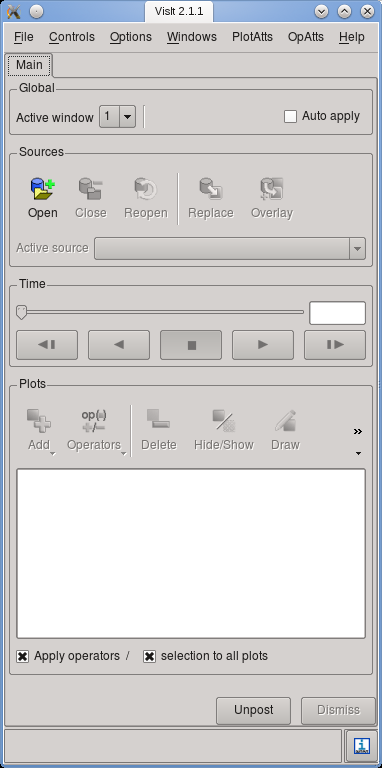
\includegraphics[width=0.24\textwidth]{viz/visit/visit-1.png}
    \label{fig:visit-1:a}
  }
  \hfill
  \subfigure[]{
    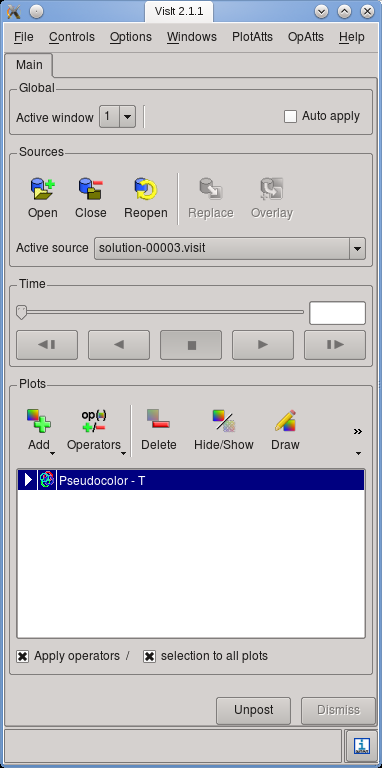
\includegraphics[width=0.24\textwidth]{viz/visit/visit-2.png}
    \label{fig:visit-1:b}
  }
  \hfill
  \subfigure[]{
    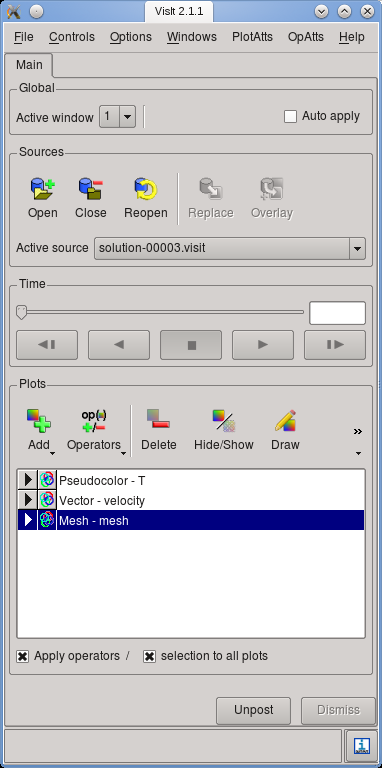
\includegraphics[width=0.24\textwidth]{viz/visit/visit-3.png}
    \label{fig:visit-1:c}
  }
  \hfill
  \phantom{.}
  \caption{\it Main window of Visit, illustrating the different steps of
    adding content to a visualization.}
  \label{fig:visit-1}
\end{figure}

\begin{figure}[tbp]
  \phantom{.}
  \hfill
  \subfigure[]{
    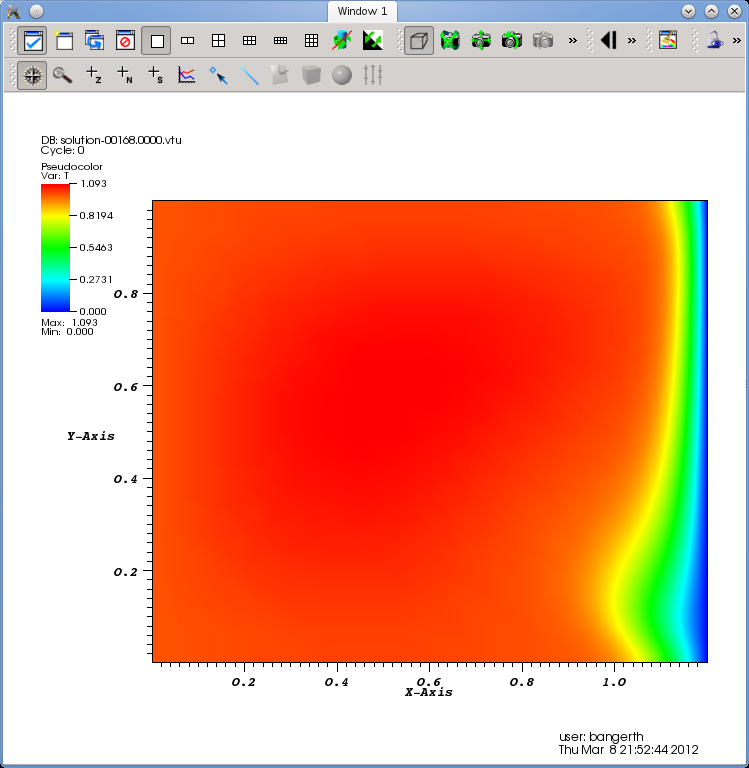
\includegraphics[width=0.48\textwidth]{viz/visit/visit-4.png}
    \label{fig:visit-2:a}
  }
  \hfill
  \subfigure[]{
    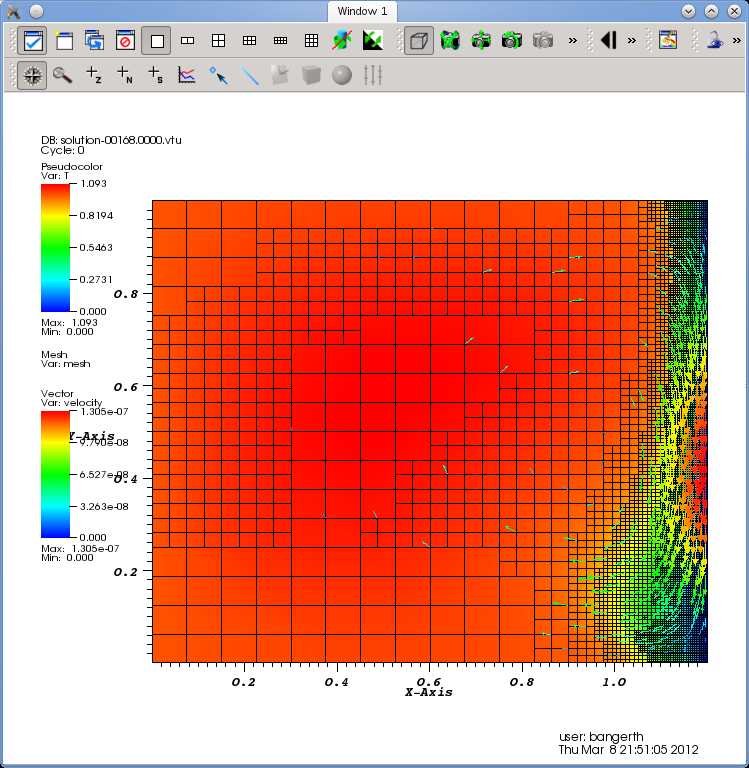
\includegraphics[width=0.48\textwidth]{viz/visit/visit-5.png}
    \label{fig:visit-2:b}
  }
  \hfill
  \phantom{.}
  \caption{\it Display window of Visit, showing a single plot and one where
    different data is overlaid.}
  \label{fig:visit-2}
\end{figure}

\begin{itemize}
\item \textit{Selecting input files:} As mentioned above, in parallel
  computations we usually generate one output file per processor in each time
  step for which visualization data is produced (see, however,
  Section~\ref{sec:viz-data}). To tell Visit which files together make up one
  time step, \aspect{} creates a \texttt{output/solution/solution-XXXXX.visit}
  file in the output directory. To open it, start Visit, click on the ``Open'' button in
  the ``Sources'' area of
  its main window (see Fig.~\ref{fig:visit-1:a}) and select the file you
  want. Alternatively, you can also select files using the ``File $>$ Open''
  menu item, or hit the corresponding keyboard short-cut. After adding an
  input source, the ``Sources'' area of the main window should list the
  selected file name. More easily, you can also just open
  \texttt{output/solution.visit} which references \textit{all} output files for
  all time steps. If you open this, Visit will display a slider that allows you
  to select which time step you want to visualize, along with forward, backward,
  and play buttons that allow you to move between time steps.

\item \textit{Selecting what to plot:} \aspect{} outputs all sorts of
  quantities that characterize the solution, such as temperature, pressure,
  velocity, and many others on demand (see
  Section~\ref{parameters:Postprocess/Visualization}). Once an input file has
  been opened, you will want to add graphical representations of some of this
  data to the still empty canvas. To this end, click on the ``Add'' button of
  the ``Plots'' area. The resulting menu provides a number of different kinds
  of plots. The most important for our purpose are: (i) ``Pseudocolor'' allows
  the visualization of a scalar field (e.g., temperature, pressure, density)
  by using a color field. (ii) ``Vector'' displays a vector-valued field
  (e.g., velocity) using arrows. (iii) ``Mesh'' displays the mesh. The
  ``Contour'', ``Streamline'' and ``Volume'' options are also frequently
  useful, in particular in 3d.

  Let us choose the ``Pseudocolor'' item and select the temperature field as
  the quantity to plot. Your main window should now look as shown in
  Fig.~\ref{fig:visit-1:b}. Then hit the ``Draw'' button to make Visit generate
  data for the selected plots. This will yield a picture such as shown in
  Fig.~\ref{fig:visit-2:a} in the display window of Visit.

\item \textit{Overlaying data:} Visit can overlay multiple plots in the same
  view. To this end, add another plot to the view using again the ``Add''
  button to obtain the menu of possible plots, then the ``Draw'' button to
  actually draw things. For example, if we add velocity vectors and the mesh,
  the main window looks as in Fig.~\ref{fig:visit-1:c} and the main view as in
  Fig.~\ref{fig:visit-2:b}.

\item \textit{Adjusting how data is displayed:} Without going into too much
  detail, if you double click onto the name of a plot in the ``Plots'' window,
  you get a dialog in which many of the properties of this plot can be
  adjusted. Further details can be changed by using ``Operators'' on a plot.

\item \textit{Making the output prettier:} As can be seen in
  Fig.~\ref{fig:visit-2}, Visit by default puts a lot of clutter around the
  figure -- the name of the user, the name of the input file, color bars, axes
  labels and ticks, etc. This may be useful to explore data in the beginning
  but does not yield good pictures for presentations or publications. To
  reduce the amount of information displayed, go to the ``Controls $>$
  Annotations'' menu item to get a dialog in which all of these displays can
  be selectively switched on and off.

\item \textit{Saving figures:} To save a visualization into a file that can
  then be included into presentations and publications, go to the menu item
  ``File $>$ Save window''. This will create successively numbered files in
  the directory from which Visit was started each time a view is saved. Things
  like the format used for these files can be chosen using the ``File $>$ Set
  save options'' menu item. We have found that one can often get better
  looking pictures by selecting the ``Screenshot'' method in this dialog.
\end{itemize}

More information on all of these topics can be found in the Visit
documentation, see \url{https://visit.llnl.gov/}. We have also recorded
video lectures demonstrating this process interactively at
\url{http://www.youtube.com/watch?v=3ChnUxqtt08} for Visit, and at
\url{http://www.youtube.com/watch?v=w-65jufR-bc} for ParaView.


\subsubsection{Visualizing statistical data}
\label{sec:viz-stat}

In addition to the graphical output discussed above, \aspect{} produces a
statistics file that collects information produced during each time step.
For the remainder of this section, let us assume that we have run \aspect{}
with the input file discussed in Section~\ref{sec:cookbooks-simple-box},
simulating convection in a box. After running \aspect{}, you will find
a file called \texttt{statistics} in the output directory that, at the time
of writing this, looked like this:
This file has a structure that looks (at the time of writing this section)
like this:
\begin{lstlisting}[frame=single,language=ksh,showstringspaces=false]
# 1: Time step number
# 2: Time (seconds)
# 3: Number of mesh cells
# 4: Number of Stokes degrees of freedom
# 5: Number of temperature degrees of freedom
# 6: Iterations for temperature solver
# 7: Iterations for Stokes solver
# 8: Velocity iterations in Stokes preconditioner
# 9: Schur complement iterations in Stokes preconditioner
# 10: Time step size (seconds)
# 11: RMS velocity (m/s)
# 12: Max. velocity (m/s)
# 13: Minimal temperature (K)
# 14: Average temperature (K)
# 15: Maximal temperature (K)
# 16: Average nondimensional temperature (K)
# 17: Outward heat flux through boundary with indicator 0 ("left") (W)
# 18: Outward heat flux through boundary with indicator 1 ("right") (W)
# 19: Outward heat flux through boundary with indicator 2 ("bottom") (W)
# 20: Outward heat flux through boundary with indicator 3 ("top") (W)
# 21: Visualization file name
 0 0.0000e+00 256 2467 1089  0 29 30 29 1.2268e-02 1.79026783e+00 2.54322608e+00
 1 1.2268e-02 256 2467 1089 32 29 30 30 3.7388e-03 5.89844152e+00 8.35160076e+00
 2 1.6007e-02 256 2467 1089 20 28 29 29 2.0239e-03 1.09071922e+01 1.54298908e+01
 3 1.8031e-02 256 2467 1089 15 27 28 28 1.3644e-03 1.61759153e+01 2.28931189e+01
 4 1.9395e-02 256 2467 1089 13 26 27 27 1.0284e-03 2.14465789e+01 3.03731397e+01
 5 2.0424e-02 256 2467 1089 11 25 26 26 8.2812e-04 2.66110761e+01 3.77180480e+01
 \end{lstlisting}

In other words, it first lists what the individual columns mean with a hash
mark at the beginning of the line and then has one line for each time step
in which the individual columns list what has been explained above.%
\footnote{With
  input files that ask for initial adaptive refinement, the first time step may
  appear twice because we solve on a mesh
  that is globally refined and we then start the entire computation
  over again on a once adaptively refined mesh (see the parameters in
  Section~\ref{parameters:Mesh_20refinement} for how to do that).}

This file is easy to visualize. For example, one can import it as a whitespace
separated file into a spreadsheet such as Microsoft Excel or OpenOffice/LibreOffice
Calc and then generate graphs of one column against another. Or, maybe simpler,
there is a multitude of simple graphing programs that do not need the overhead
of a full fledged spreadsheet engine and simply plot graphs. One that is
particularly simple to use and available on every major platform is \texttt{Gnuplot}.
It is extensively documented at \url{http://www.gnuplot.info/}.

\texttt{Gnuplot} is a command line program in which you enter commands that
plot data or modify the way data is plotted. When you call it, you will first
get a screen that looks like this:
\begin{lstlisting}[frame=single,showstringspaces=false]
/home/user/aspect/output gnuplot

        G N U P L O T
        Version 4.6 patchlevel 0    last modified 2012-03-04
        Build System: Linux x86_64

        Copyright (C) 1986-1993, 1998, 2004, 2007-2012
        Thomas Williams, Colin Kelley and many others

        gnuplot home:     http://www.gnuplot.info
        faq, bugs, etc:   type "help FAQ"
        immediate help:   type "help"  (plot window: hit 'h')

Terminal type set to 'qt'
gnuplot>
\end{lstlisting}
At the prompt on the last line, you can then enter commands. Given the
description of the individual columns given above, let us first try to
plot the heat flux through boundary 2 (the bottom
boundary of the box), i.e., column 19, as a function of time (column 2).
This can be achieved using the following command:
\begin{lstlisting}[frame=single,language=gnuplot,showstringspaces=false]
  plot "statistics" using 2:19
\end{lstlisting}
The left panel of Fig.~\ref{fig:viz-gnuplot-1} shows what \texttt{Gnuplot}
will display in its output window. There are many things one can
configure in these plots (see the \texttt{Gnuplot} manual referenced above).
For example, let us assume that we want to add labels to the $x$- and $y$-axes,
use not just points but lines and points for the curves,
restrict the time axis to the range $[0,0.2]$ and the heat flux axis to
$[-10:10]$,
plot not only the flux through the bottom but also through the top boundary
(column 20) and finally add a key to the figure, then the following
commands achieve this:
\begin{lstlisting}[frame=single,language=gnuplot,showstringspaces=false]
  set xlabel "Time"
  set ylabel "Heat flux"
  set style data linespoints
  plot [0:0.2][-10:10] "statistics" using 2:19 title "Bottom boundary", \
                       "statistics" using 2:20 title "Top boundary"
\end{lstlisting}
If a line gets too long, you can continue it by ending it in a backslash as
above. This is rarely used on the command line but useful when writing the
commands above into a script file, see below. We have done it here to get
the entire command into the width of the page.

\begin{figure}
  \centering
  \phantom.
  \hfill
  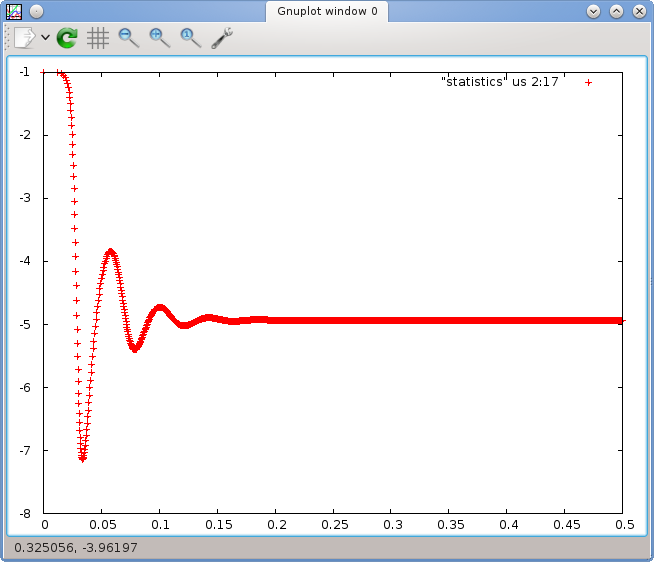
\includegraphics[width=0.4\textwidth]{viz/statistics/1.png}
  \hfill
  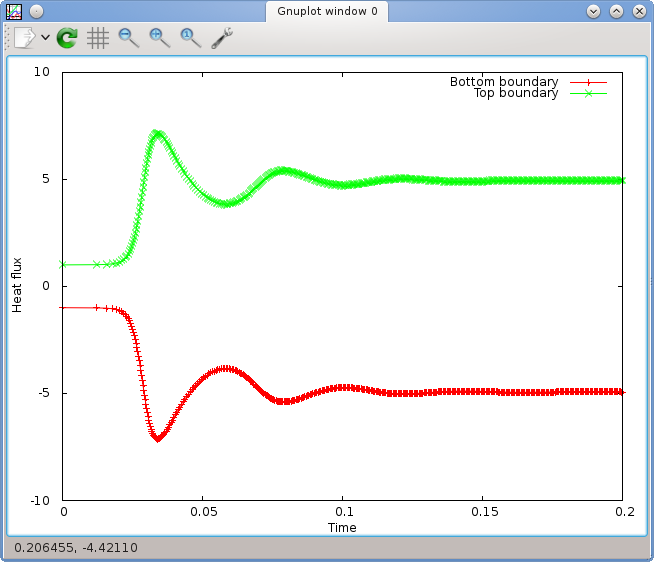
\includegraphics[width=0.4\textwidth]{viz/statistics/2.png}
  \hfill
  \phantom.
  \caption{\it Visualizing the statistics file obtained from the example in
    Section~\ref{sec:cookbooks-simple-box} using \texttt{Gnuplot}: Output
    using simple commands.}
  \label{fig:viz-gnuplot-1}
\end{figure}

For those who are lazy, \texttt{Gnuplot} allows to abbreviate things in many
different ways. For example, one can abbreviate most commands. Furthermore,
one does not need to repeat the name of an input file if it is the same
as the previous one in a plot command. Thus, instead of the commands above,
the following abbreviated form would have achieved the same effect:
\begin{lstlisting}[frame=single,language=gnuplot,showstringspaces=false]
  se xl "Time"
  se yl "Heat flux"
  se sty da lp
  pl [:0.2][-10:10] "statistics" us 2:19 t "Bottom boundary", "" us 2:20 t "Top boundary"
\end{lstlisting}
This is of course unreadable at first but becomes useful once you become
more familiar with the commands offered by this program.

Once you have gotten the commands that create the plot you want right, you probably
want to save it into a file. \texttt{Gnuplot} can write output in many
different formats. For inclusion in publications, either \texttt{eps} or
\texttt{png} are the most common. In the latter case, the commands to
achieve this are
\begin{lstlisting}[frame=single,language=gnuplot,showstringspaces=false]
  set terminal png
  set output "heatflux.png"
  replot
\end{lstlisting}
The last command will simply generate the same plot again but this time
into the given file. The result is a graphics file similar to the one
shown in Fig.~\ref{fig:convection-box-stats} on page \pageref{fig:convection-box-stats}.

\note{After setting output to a file, \textit{all} following plot commands will
  want to write to this file. Thus, if you want to create more plots after
  the one just created, you need to reset output back to the screen. On Linux,
  this is done using the command \texttt{set terminal X11}. You can then
  continue experimenting with plots and when you have the next plot ready,
  switch back to output to a file.}

What makes \texttt{Gnuplot} so useful is that it doesn't just allow entering
all these commands at the prompt. Rather, one can write them all into a file,
say \texttt{plot-heatflux.gnuplot}, and then, on the command line, call
\begin{lstlisting}[frame=single,language=ksh]
  gnuplot plot-heatflux.gnuplot
\end{lstlisting}
to generate the \texttt{heatflux.png} file. This comes in handy if one wants
to create the same plot for multiple simulations while playing with parameters
of the physical setup. It is also a very useful tool if one wants to generate
the same kind of plot again later with a different data set, for example when
a reviewer requested additional computations to be made for a paper or if one
realizes that one has forgotten or misspelled an axis label in a plot.%
\footnote{In my own work, I usually save the \aspect{} input file, the
  \texttt{statistics} output file and the \texttt{Gnuplot} script along with
  the actual figure I want to include in a paper. This way, it is easy to
  either re-run an entire simulation, or just tweak the graphic at a later
  time. Speaking from experience, you will not believe how often one wants
  to tweak a figure long after it was first created. In such situations it is
  outstandingly helpful if one still has both the actual data as well as the script
  that generated the graphic.}

\texttt{Gnuplot} has many many more features we have not even touched upon. For
example, it is equally happy to produce three-dimensional graphics, and it also
has statistics modules that can do things like curve fits, statistical regression,
and many more operations on the data you provide in the columns of an input file.
We will not try to cover them here but instead refer to the manual at
\url{http://www.gnuplot.info/}. You can also get a good amount of information
by typing \texttt{help} at the prompt, or a command like \texttt{help plot} to
get help on the \texttt{plot} command.


\subsubsection{Large data issues for parallel computations}
\label{sec:viz-data}

Among the challenges in visualizing the results of parallel computations is
dealing with the large amount of data. The first bottleneck this presents is
during run-time when \aspect{} wants to write the visualization data of a time
step to disk. Using the compressed VTU format, \aspect{} generates on the
order of 10 bytes of output for each degree of freedom in 2d and more in 3d;
thus, output of a single time step can run into the range of gigabytes that
somehow have to get from compute nodes to disk. This stresses both the cluster
interconnect as well as the data storage array.
\index[prmindex]{Number of grouped files}
\index[prmindexfull]{Postprocess!Visualization!Number of grouped files}


There are essentially two strategies supported by \aspect{} for this scenario:
\begin{itemize}
\item If your cluster has a fast interconnect, for example Infiniband, and if
  your cluster has a fast, distributed file system, then \aspect{} can produce
  output files that are already located in the correct output directory (see
  the options in Section~\ref{parameters:global}) on the global file
  system. \aspect{} uses MPI I/O calls to this end, ensuring that the local
  machines do not have to access these files using slow NFS-mounted global
  file systems.

\item If your cluster has a slow interconnect, e.g., if it is simply a
  collection of machines connected via Ethernet, then writing data to a
  central file server may block the rest of the program for a while. On the
  other hand, if your machines have fast local storage for temporary file
  systems, then \aspect{} can write data first into such a file and then move
  it in the background to its final destination while already continuing
  computations. To select this mode, set the appropriate variables discussed
  in Section~\ref{parameters:Postprocess/Visualization}. Note, however, that
  this scheme only makes sense if every machine on which MPI processes run has
  fast local disk space for temporary storage.
\end{itemize}

\note{An alternative would be if every processor directly writes its own files
  into the global output directory (possibly in the background), without the
  intermediate step of the temporary file. In our experience, file servers are
  quickly overwhelmed when encountering a few hundred machines wanting to
  open, fill, flush and close their own file via NFS mounted file system
  calls, sometimes completely blocking the entire cluster environment for
  extended periods of time.}

\subsection{Checkpoint/restart support}
\label{sec:checkpoint-restart}

If you do long runs, especially when using parallel computations, there are a
number of reasons to periodically save the state of the program:
\begin{itemize}
\item If the program crashes for whatever reason, the entire computation may
  be lost. A typical reason is that a program has exceeded the requested
  wallclock time allocated by a batch scheduler on a cluster.
\item Most of the time, no realistic initial conditions for strongly
  convecting flow are available. Consequently, one typically starts with a
  somewhat artificial state and simply waits for a long while till the
  convective state enters the phase where it shows its long-term
  behavior. However, getting there may take a good amount of CPU time and it
  would be silly to always start from scratch for each different parameter
  setting. Rather, one would like to start such parameter studies with a saved
  state that has already passed this initial, unphysical, transient stage.
\end{itemize}

To this end, \aspect{} creates a set of files in the output directory
\index[prmindex]{Output directory}
\index[prmindexfull]{Output directory}
(selected in the parameter file) every N time steps (controlled by the number
of steps or wall time as specified in \texttt{subsection Checkpointing}, see
Section~\ref{parameters:Checkpointing}) in which the entire state of the
program is saved so that a simulation can later be continued at this
point. The previous checkpoint files will then be deleted. To resume
operations from the last saved state, you need to set the \texttt{Resume
  computation} flag in the input parameter file to \texttt{true}, see
\index[prmindex]{Resume computation}
\index[prmindexfull]{Resume computation}
Section~\ref{parameters:Resume computation}.

\note{It is not imperative that the parameters selected in the input file are
  exactly the same when resuming a program from a saved state than what they
  were at the time when this state was saved. For example, one may want to
  choose a different parameterization of the material law, or add or remove
  postprocessors that should be run at the end of each time step. Likewise,
  the end time, the times at which some additional mesh refinement steps
  should happen, etc., can be different.

  Yet, it is
  clear that some other things can't be changed: For example, the geometry
  model that was used to generate the coarse mesh and describe the boundary
  must be the same before and after resuming a computation. Likewise, you can
  not currently restart a computation with a different number of processors
  than initially used to checkpoint the simulation.
  Not all invalid
  combinations are easy to detect, and \aspect{} may not always realize
  immediate what is going on if you change a setting that can't be
  changed. However, you will almost invariably get nonsensical results after
  some time.}


\subsection{Making \aspect{} run faster}

When developing \aspect{}, we are guided by the principle that the default for
all settings should be \textit{safe}. In particular, this means that you should
get errors when something goes wrong, the program should not let you choose an
input file parameter so that it doesn't make any sense, and we should solve the
equations to best ability without cutting corners. The goal is that when you
start working with \aspect{} that we give you the best answer we can. The
downside is that this also makes \aspect{} run slower than may be possible. This
section describes ways of making \aspect{} run faster -- assuming that you know
what you are doing and are making conscious decisions.

\subsubsection{Debug vs.~optimized mode}
Both \dealii{} and \aspect{} by default have a great deal of internal checking
to make sure that the code's state is valid. For example, if you write a new
postprocessing plugin (see Section~\ref{sec:plugins})) in which you need to
access the solution vector, then \dealii{}'s \texttt{Vector} class will make
sure that you are only accessing elements of the vector that actually exist and
are available on the current machine if this is a parallel computation. We do so
because it turns out that by far the most bugs one introduces in programs are of
the kind where one tries to do something that obviously doesn't make sense
(such as accessing vector element 101 when it only has 100 elements). These
kinds of bugs are more frequent than implementing a wrong algorithm, but they
are fortunately easy to find if you have a sufficient number of assertions in
your code. The downside is that assertions cost run time.

As mentioned above, the default is to have all of these assertions in the code
to catch those places where we may otherwise silently access invalid memory
locations. However, once you have a plugin running and verified that your input
file runs without problems, you can switch off all of these checks by switching
from debug to optimized mode. This means re-compiling \aspect{} and linking
against a version of the \dealii{} library without all of these internal checks.
Because this is the first thing you will likely want to do, we have already
discussed how to do all of this in Section~\ref{sec:debug-mode}.

\subsubsection{Adjusting solver tolerances} At the heart of every time step
lies the solution of linear systems for the Stokes equations, the temperature
field, and possibly for compositional fields. In essence, each of these steps
requires us to solve a linear system of the form $Ax=b$ which we do through
iterative solvers, i.e., we try to find a sequence of approximations $x^{(k)}$
where $x^{(k)}\rightarrow x=A^{-1}b$. This iteration is terminated at iteration
$k$ if the approximation is ``close enough'' to the exact solution. The solvers
we use determine this by testing after every iteration whether the
\textit{residual}, $r^{(k)}=A(x-x^{(k)})=b-Ax^{(k)}$, satisfies
$\|r^{(k)}\|\le\varepsilon\|r^{(0)}\|$ where $\varepsilon$ is called the
(relative) \textit{tolerance}.

Obviously, the smaller we choose $\varepsilon$, the more accurate the
approximation $x^{(k)}$ will be. On the other hand, it will also take more
iterations and, consequently, more CPU time to reach the stopping criterion with
a smaller tolerance. The default value of these tolerances are chosen so that
the approximation is typically sufficient. You can make \aspect{} run faster if
you choose these tolerances larger.
The parameters you can adjust are all listed in
Section~\ref{parameters:Solver_20parameters} and are located in the \texttt{Solver parameters} subsection of the input
file. In particular, the parameters you want to look at are \texttt{Linear
solver tolerance}, \texttt{Temperature solver tolerance} and
\texttt{Composition solver tolerance}.
\index[prmindex]{Composition solver tolerance}
\index[prmindexfull]{Composition solver tolerance}
\index[prmindex]{Linear solver tolerance}
\index[prmindexfull]{Linear solver tolerance}
\index[prmindex]{Temperature solver tolerance}
\index[prmindexfull]{Temperature solver tolerance}

All this said, it is important to understand the consequences of choosing
tolerances larger. In particular, if you choose tolerances too large, then the
difference between the exact solution of a linear system $x$ and the
approximation $x^{(k)}$ may become so large that you do not get an accurate
output of your model any more. A rule of thumb in choosing tolerances is to
start with a small value and then increase the tolerance until you come to a
point where the output quantities start to change significantly. This is the
point where you will want to stop.

\subsubsection{Adjusting solver preconditioner tolerances} To solve the Stokes
equations it is necessary to lower the condition number of the
Stokes matrix by preconditioning  it. In \aspect{} a right preconditioner $Y^{-1} =
\begin{pmatrix}
\widetilde{A^{-1}} & -\widetilde{A^{-1}}B^{T}\widetilde{S^{-1}} \\
0 & \widetilde{S^{-1}}
\end{pmatrix}$ is used to precondition the system, where $\widetilde{A^{-1}}$ is
the approximate inverse of the A block and $\widetilde{S^{-1}}$ is the approximate
inverse of the Schur complement matrix. Matrix $\widetilde{A^{-1}}$ and
$\widetilde{S^{-1}}$ are calculated through a CG solve, which requires a tolerance
to be set. In comparison with the solver tolerances of the previous section, these
parameters are relatively safe to use, since they only change the preconditioner,
but can speed up or slow down solving the Stokes system considerably.

In practice $\widetilde{A^{-1}}$ takes by far the most time to compute, but is
also very important in conditioning the system. The accuracy of the computation
of $\widetilde{A^{-1}}$ is controlled by the parameter \texttt{Linear solver A
block tolerance} which has a default value of $1e-2$. Setting this tolerance
to a less strict value will result in more outer iterations, since the
preconditioner is not as good, but the amount of time to compute
$\widetilde{A^{-1}}$ can drop significantly resulting in a reduced total solve
time. The cookbook crustal deformation (Section
\ref{sec:cookbooks-crustal-deformation}) for example can be computed much faster
by setting the \texttt{Linear solver A block tolerance} to $5e-1$. The
calculation of $\widetilde{S^{-1}}$ is usually much faster and the
conditioning of the system is less sensitive to the parameter \texttt{Linear
solver S block tolerance}, but for some problems it might be worth it to
investigate.
\index[prmindex]{Linear solver A block tolerance}
\index[prmindexfull]{Linear solver A block tolerance}
\index[prmindex]{Linear solver S block tolerance}
\index[prmindexfull]{Linear solver S block tolerance}

\subsubsection{Using lower order elements for the temperature/compositional discretization}
The default settings of \aspect{} use quadratic finite elements for the
velocity. Given that the temperature and compositional fields essentially (up
to material parameters) satisfy advection equations of the kind $\partial_t T +
\mathbf u \cdot \nabla T = \ldots$, it seems appropriate to also use quadratic
finite element shape functions for the temperature and compositional fields.

However, this is not mandatory. If you do not care about high accuracy in these
fields and are mostly interested in the velocity or pressure field, you can
select lower-order finite elements in the input file. The polynomial degrees are
controlled with the parameters in the \textit{discretization} section of the
input file, see Section~\ref{parameters:Discretization}, in particular by
\texttt{Temperature polynomial degree} and
\texttt{Composition polynomial degree}.
\index[prmindex]{Temperature polynomial degree}
\index[prmindexfull]{Discretization!Temperature polynomial degree}
\index[prmindex]{Composition polynomial degree}
\index[prmindexfull]{Discretization!Composition polynomial degree}

As with the other parameters discussed above and below, it is worthwhile
comparing the results you get with different values of these parameters when
making a decision whether you want to save on accuracy in order to reduce
compute time. An example of how this choice affects the accuracy you get is
discussed in Section~\ref{sec:cookbooks-simple-box}.



\subsubsection{Limiting postprocessing}
\aspect{} has a lot of postprocessing capabilities, from generating graphical
output to computing average temperatures or temperature fluxes. To see what all
is possible, take a look at the \texttt{List of postprocessors} parameter that
can be set in the input file, see Section~\ref{parameters:Postprocess}.
\index[prmindex]{List of postprocessors}
\index[prmindexfull]{Postprocess!List of postprocessors}

Many of these postprocessors take a non-negligible amount of time. How much they
collectively use can be inferred from the timing report \aspect{} prints
periodically among its output, see for example the output shown in
Section~\ref{sec:cookbooks-simple-box}. So, if your computations take too long,
consider limiting which postprocessors you run to those you really need. Some
postprocessors -- for example those that generate graphical output, see
Section~\ref{parameters:Postprocess/Visualization} -- also allow you to run them
only once every once in a while, rather than at every time step.


\subsubsection{Switching off pressure normalization}
In most practically relevant cases, the Stokes equations
\eqref{eq:stokes-1}--\eqref{eq:stokes-2} only determine the pressure up to a
constant because only the pressure gradient appears in the equations, not the
actual value of it. However, unlike this ``mathematical'' pressure, we have a
very specific notion of the ``physical'' pressure: namely a well-defined
quantity that at the surface of Earth equals the air pressure, which compared to
the hydrostatic pressure inside Earth is essentially zero.

As a consequence, the default in \aspect{} is to normalize the computed
``mathematical'' pressure in such a way that either the mean pressure at the
surface is zero (where the geometry model describes where the ``surface'' is,
see Section~\ref{sec:geometry-models}), or that the mean pressure in the domain
is zero. This normalization is important if your model describes densities,
viscosities and other quantities in dependence of the pressure -- because you
almost certainly had the ``physical'' pressure in mind, not some unspecified
``mathematical'' one. On the other hand, if you have a material model in which
the pressure does not enter, then you don't need to normalize the pressure at
all -- simply go with whatever the solver provides. In that case, you can switch
off pressure normalization by looking at the \texttt{Pressure normalization}
parameter at the top level of the input file, see
Section~\ref{parameters:global}.
\index[prmindex]{Pressure normalization}
\index[prmindexfull]{Pressure normalization}


\subsubsection{Regularizing models with large coefficient variation}
Models with large jumps in viscosity and other coefficients present
significant challenges to both discretizations and solvers. In particular,
they can lead to very long solver
times. Section~\ref{sec:sinker-with-averaging} presents parameters that can
help regularize models and these typically also include significant
improvements in run-time.
\index[prmindex]{Material averaging}
\index[prmindexfull]{Material model!Material averaging}


\subsubsection{Using multithreading}
In most cases using as many MPI processes as possible is the optimal
parallelization strategy for \aspect{} models, but if you are limited by the
amount of MPI communication it can be beneficial to use multiple threads per
MPI process. While not utilized by our linear solvers, this parallelization can
speed up the assembly of the system matrices, e.g. by around 10-15\% if you
utilize unused logical cores, or nearly linearly if you use otherwise
unused physical cores. This can also reduce the performance cost if you are
memory limited and need to run your model on less than the available number of
cores per node on a cluster to increase the available memory per core.  Running
with for example two threads per process will offset some of the performance
loss you will see in these situations.

Multithreading is controlled by setting the command line parameter \texttt{-j}
or \texttt{-{}-threads}. If the parameter is not set, \aspect{} will create
exactly one thread per MPI process, i.e. multithreading is disabled.  Appending
the parameter allows \aspect{} to spawn several threads per MPI process. Note
that the internally used TBB library will determine the number of threads based
on the number of available cores, i.e., if you start 2~MPI processes on a
quadcore machine with hyperthreading (8 logical cores), \aspect{} will spawn 4
threads on each MPI process. Also note that there is no guarantee that the
final number of threads will exactly match the number of available logical
cores if you start with a number of processes that is not a divisor of your
logical cores (e.g. 3 MPI processes for 8 logical cores).

\subsection{Input parameter files}
\label{sec:parameters-overview}

What \aspect{} computes is driven by two things:
\begin{itemize}
\item The models implemented in \aspect{}. This includes the geometries, the
  material laws, or the initial conditions currently supported. Which of these
  models are currently implemented is discussed below;
  Section~\ref{sec:extending} discusses in great detail the process of
  implementing additional models.

\item Which of the implemented models is selected, and what their run-time
  parameters are. For example, you could select a model that prescribes
  constant coefficients throughout the domain from all the material models
  currently implemented; you could then select appropriate values for all of
  these constants. Both of these selections happen from a parameter file that
  is read at run time and whose name is specified on the command line. (See
  also Section~\ref{sec:running-overview}.)
\end{itemize}
In this section, let us give an overview of what can be selected in the
parameter file. Specific parameters, their default values, and allowed values
for these parameters are documented in Section~\ref{sec:parameters}. An index
with page numbers for all run-time parameters can be found on
page~\pageref{sec:runtime-parameter-index}.

\subsubsection{The structure of parameter files}

Most of the run-time behavior of \aspect{} is driven by a parameter file that
looks in essence like this:
\lstinputlisting[language=prmfile]{cookbooks/overview/doc/structure.part.prm.out}

Some parameters live at the top level, but most parameters are grouped into
subsections. An input parameter file is therefore much like a file system: a
few files live in the root directory; others are in a nested hierarchy of
sub-directories. And just as with files, parameters have both a name (the
thing to the left of the equals sign) and a content (what's to the right).

All parameters you can list in this input file have been \textit{declared} in
\aspect. What this means is that you can't just list anything in the input
file, and expect that entries that are unknown are simply ignored.
Rather, if your input file contains a line setting a parameter that is unknown, you
will get an error message. Likewise, all declared parameters have a
description of possible values associated with them -- for example, some
parameters must be non-negative integers (the number of initial refinement
steps), can either be true or false (whether the computation should be resumed
from a saved state), or can only be a single element from a selection (the
name of the material model). If an entry in your input file doesn't satisfy
these constraints, it will be rejected at the time of reading the file (and
not when a part of the program actually accesses the value and the programmer
has taken the time to also implement some error checking at this location).
Finally, because parameters have been declared, you do not \textit{need} to
specify a parameter in the input file: if a parameter isn't listed, then the
program will simply use the default provided when declaring the parameter.

\note{In cases where a parameter requires a significant amount of text, you can
end a line in the input file with a backslash. This indicates that the
following line will simply continue to be part of the text of the current line,
in the same way as the C/C++ preprocessor expands lines that end in
backslashes. The underlying implementation always eats whitespace at
the beginning of each continuing line, but not before the
backslash. This means that the parameter file \\
\hspace*{.25cm} \texttt{set Some parameter = abc}$\backslash$ \\
\hspace*{.25cm} \texttt{\phantom{set Some parameter = }def}\\
is equivalent to \\
\hspace*{.25cm} \texttt{set Some parameter = abcdef}\\
that is, with no space between \texttt{abc} and \texttt{def} despite
the leading whitespace at the beginning of the second line. If you
do want space between these two parts, you need to add it before the
backslash in the first of the two lines.
}

\subsubsection{Categories of parameters}

The parameters that can be provided in the input file can roughly be
categorized into the following groups:
\begin{itemize}
\item Global parameters (see Section~\ref{parameters:global}): These
  parameters determine the overall behavior of the program. Primarily they
  describe things like the output directory, the end time of the simulation,
  or whether the computation should be resumed from a previously saved state.

\item Parameters for certain aspects of the numerical algorithm: These
  describe, for example, the specifics of the spatial discretization. In
  particular, this is the case for parameters concerning
  the polynomial degree of the finite element approximation
  (Section~\ref{parameters:Discretization}), some details about the
  stabilization
  (Section~\ref{parameters:Discretization/Stabilization_20parameters}), and
  how adaptive mesh refinement is supposed to work
  (Section~\ref{parameters:Mesh_20refinement}).

\item Parameters that describe certain global aspects of the equations to be
  solved: This includes, for example, a description if certain terms in the
  model should be omitted or not. See
  Section~\ref{parameters:Formulation} for the list of parameters in this
  category.

\item Parameters that characterize plugins: Certain behaviors of
  \aspect{} are described by what we call \textit{plugins} -- self-contained
  parts of the code that describe one particular aspect of the simulation. An
  example would be which of the implemented material models to use, and the
  specifics of this material model. The sample parameter file above gives an
  indication of how this works: within a subsection of the file that pertains
  to the material models, one can select one out of several plugins (or, in
  the case of the postprocessors, any number, including none, of the available
  plugins), and one can then specify the specifics of this model in a
  sub-subsection dedicated to this particular model.

  A number of components of \aspect{} are implemented via plugins. Some of
  these, together with the sections in which their parameters are declared, are
  the following:
  \begin{itemize}
  \item The material model:
    Sections~\ref{parameters:Material_20model} and following.
  \item The geometry:
    Sections~\ref{parameters:Geometry_20model} and following.
  \item The gravity description:
    Sections~\ref{parameters:Gravity_20model} and following.
  \item Initial conditions for the temperature:
    Sections~\ref{parameters:Initial_20temperature_20model} and following.
  \item Temperature boundary conditions:
    Sections~\ref{parameters:Boundary_20temperature_20model} and following.
  \item Postprocessors:
    Sections~\ref{parameters:Postprocess} and following for most postprocessors,
    section \ref{parameters:Postprocess/Visualization} and following for
    postprocessors related to visualization.
  \end{itemize}
\end{itemize}

The details of parameters in each of these categories can be found in the
sections linked to above. Some of them will also be used in the cookbooks in
Section~\ref{sec:cookbooks}.


\subsubsection{A note on the syntax of formulas in input files}
\label{sec:muparser-format}

Input files have different ways of describing certain things to \aspect{}. For
example, you could select a plugin for the temperature initial values that
prescribes a constant temperature, or a
plugin that implements a particular formula for these initial conditions in
C++ in the code of the plugin, or a
plugin that allows you to describe this formula in a symbolic way in the input file
(see Section~\ref{parameters:Initial_20temperature_20model}). An example of this latter
case is this snippet of code discussed in
Section~\ref{sec:cookbooks-simple-box-3d}:
%
\lstinputlisting[language=prmfile]{../../cookbooks/convection_box_3d/doc/initial.part.prm.out}
%
The formulas you can enter here need to use a syntax that is understood by the
functions and classes that interpret what you write. Internally, this is done
using the muparser library, see \url{http://muparser.beltoforion.de/}. The
syntax is mostly self-explanatory in that it allows to use the usual symbols
\texttt{x}, \texttt{y} and \texttt{z} to reference coordinates (unless a
particular plugin uses different variables, such as the depth), the symbol
\texttt{t} for time in many situations, and allows you to use all of the
typical mathematical functions such as sine and cosine. Based on the muparser
library, deal.II supports additional functions, including \texttt{|} (the logical OR), \texttt{\&} (the logical AND),
\texttt{int()}, \texttt{ceil()}, \texttt{floor()}, \texttt{cot()},
\texttt{csc()}, \texttt{sec()}, \texttt{pow()}, \texttt{log()},
\texttt{erfc()}, \texttt{rand()}, and \texttt{rand\_seed()}.
For more detailed information, see
\url{http://www.dealii.org/developer/doxygen/deal.II/classFunctionParser.html#details}.

A common need for function expression is an if-else-statement, for example
``if $1<x<4$ then output 1, else output 0''.
The muparser uses lazy-expression syntax \texttt{(if-condition ?\ true-expression :\ false-expression )}
for if-else statements. This lazy-expression only evaluates the expression that meets the
if-condition, rather than evaluating both expressions, which can be useful if one of the
expressions is not defined (e.g., has a divide by zero) when the if-condition is not met.
Note it is also possible to use the syntax \texttt{if(condition, true-expression, false-expression)},
but in this case both expressions are always evaluated. This is inefficient, but in addition may abort the program with a floating point exception if the expression that will be discarded has invalid floating point operations (such as a division by zero, or taking the square root of a negative number) that would ordinarily not be visible because, after all, the expression should be discarded.
Therefore, the lazy-expression syntax is recommended.

As a simple example using the lazy-expression syntax, the statement ``if $1<x<4$ then output 1, else output 0''
can be expressed as \texttt{(1<x\ \&\&\ x<4 ?\ 1\ :\ 0)}.  Multiple, nested if-else expressions
can also be used. To extend the simple example, the statement
``if $1<x<4$ then, if 2<y<3, then output 2, else output 1, else output 0''
can be expressed as \texttt{((1<x\ \&\&\ x<4)\ ?\ ((2<y\ \&\&\ y<3)\ ?\ 2\ :\ 1)\ :\ (0))}.

An example for how to translate nested if-else statements into the lazy-expression syntax is given in the
cookbook example found in Section~\ref{sec:lazy-expression}. This cookbook includes a python script that defines
the initial temperature structure using nested if-else statements and shows how this is then rewritten
using the lazy-expression. The cookbook runs a single time-step to show the outcome of using the function
option for the initial temperature. Quite complex initial conditions can be defined in this way, however,
using something like python to debug these expressions before defining them in the parameter file is
recommended. For more examples of functions used in parameter files, go to the \texttt{cookbooks}
directory and use grep to search for ``Function expression'' in the parameters files.
You can also search ``Function expression'' on the \aspect{} github page.
For more examples of the syntax understood, reference the documentation of the muparser library
linked to above.

\subsubsection{Compatibility of input files with newer \aspect{} versions}

We strive to maintain compatibility for options in input files as long as
possible. However, occasionally we have to reorder, rename, or remove options
from parameter files to improve \aspect{} further. This is especially true
for new major versions. In order to allow running old parameter files with
newer \aspect{} versions we provide scripts that can automatically update
existing parameter files to the new syntax. Executing
\texttt{doc/update\_prm\_files.sh} with one or more parameter files as
arguments will create a backup of the old parameter file (named
\texttt{old\_filename.bak}), and replace the existing file with a version that
should work with the current \aspect{} version. Using this script would look
like this:

\begin{lstlisting}[frame=single,language=ksh,showstringspaces=false]
bash contrib/utilities/update_prm_files.sh cookbooks/convection_box.prm
\end{lstlisting}

\note{Not all text replacements are unique, and the structure of input files
allows for constructions the script can not properly parse. Also we can not
guarantee to preserve the structure and position of comments, as it is not
always clear to which part of the input file they refer. Thus, it is important
that you check your updated input file for errors. That being said, all input
files in the main \aspect{} repository are updated successfully using this
script.}

\subsection{A graphical user interface for editing \aspect{} parameter files}
Preparing a parameter file in a text editor can be a tedious task, not
only because the number of input parameters has grown considerably during the
development of \aspect{}, but also because remembering the names of commonly
used options is a waste of (human) memory. Therefore, we provide a graphical
user interface that builds upon an available program for \dealii{}. This GUI
allows to investigate existing input parameters, including their default values, modify
these values in a spreadsheet like environment and then save a formatted
parameter file that can be used to start an ASPECT model. In the following
subsections we describe installing and using this user interface.

\subsubsection{Installing parameter-GUI}
The \dealii{} parameter-GUI program can be downloaded at \url{https://github.com/dealii/parameter_gui},
and is compiled using the \texttt{cmake} program just like \aspect{} itself. The program has no
dependencies except for the Qt development libraries that should be available as packages for
most Linux distributions and can also be obtained for all major operating systems at
\url{https://www.qt.io/download-open-source/}.

Example steps for installing the parameter-gui could look as follows:
\begin{enumerate}
\item Download the program from \url{https://github.com/dealii/parameter_gui}.
\item Prepare a Makefile by running \texttt{cmake .} in the source folder.
\item Compile the program by running \texttt{make}.
\item Make sure to set the environment variable \texttt{PARAMETER\_GUI\_DIR}
to the directory that contains the parameter-GUI executable (optional).
This will allow \aspect{} to automatically enable the GUI during configuration.
\end{enumerate}

\paragraph{Installing on macOS} On a mac machine with recent macOS Sierra 10.12.4, Qt development libraries of version 4.x.x at the libraries' official website \url{https://www.qt.io/download-open-source/} may fail to install.  Alternatively, you can install \texttt{qt4} through Homebrew (also see instruction here \url{https://github.com/cartr/homebrew-qt4})
\begin{verbatim}
brew tap cartr/qt4
brew tap-pin cartr/qt4
brew install qt@4
\end{verbatim}
or install it through Mac Ports (\url{https://www.macports.org/})
\begin{verbatim}
sudo port install qt4-mac
\end{verbatim}
Then you can follow the Linux user instructions provided previously to download and install dealii parameter-GUI.
Before running \texttt{cmake .}, you may need to either pass the path of \texttt{qt4} and specify the value of variable \texttt{QT\_LIBRARIES} to the directory that contains the libraries of \texttt{qt4}
or add those information into your \texttt{.bash\_profile}. For example, for installation through Mac Ports, you can set the following into your \texttt{.bash\_profile}
\begin{verbatim}
export PATH="$PATH:/opt/local/libexec/qt4"
export QT_LIBRARIES="/opt/local/libexec/qt4"
\end{verbatim}




\subsubsection{Using \aspect{}-GUI}

When configuring \aspect{} after executing the above steps, it should automatically pick up the
location of the parameter-GUI, and will create a new script named \texttt{aspect-gui} within the build folder.
If this does not happen, it is possible to hand over the location of the parameter-GUI as a cmake
variable during configuration (e.g. \texttt{cmake -D PARAMETER\_GUI\_EXECUTABLE=path\_to\_your\_executable}).

The aspect-gui script can be executed from any folder either with no argument or with one argument that contains the path to
an existing parameter file. The script will run \aspect{} with the given (or an empty) parameter file, generate a database
of existing input parameters, and open the parameter-GUI program with this database. The resulting window looks similar to Fig.~\ref{fig:aspect-gui}. If an existing parameter file was
given, all parameter fields are pre-filled with the values set in the file instead of the default values.
In the program's main window you can change parameters as necessary, and then save the file as a new parameter file. This parameter file can then be used
to start an \aspect{} model as usual. Note that it is possible to prepare and execute the parameter file with different versions of \aspect{}, e.g. if you prepare parameter files on a local machine, and execute the model on a remote compute cluster.
Note however that if the two \aspect{} versions contain different default values or parameter names have changed, this can lead
to unexpected model behavior or even unusable parameter files.

\begin{figure}
\hfill
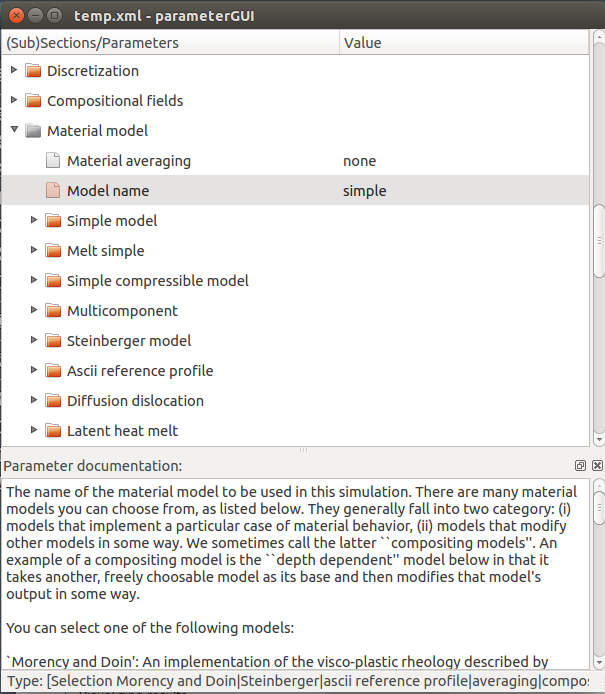
\includegraphics[width=0.4\textwidth]{aspect-gui.png}
\hfill
\phantom.
\caption{\it The parameter GUI lists all available parameter options, and allows to change and save them into a new parameter file. Input fields know about the type of the variable and will display useful options to change them (e.g. drop-down menus, file dialogs, text fields).}
\label{fig:aspect-gui}
\end{figure}

\section{Cookbooks}
\label{sec:cookbooks}

In this section, let us present a number of ``cookbooks'' -- examples of how
to use \aspect{} in typical or less typical ways. As discussed in
Sections~\ref{sec:running} and \ref{sec:parameters}, \aspect{} is driven by
run-time parameter files, and so setting up a particular situation primarily
comes down to creating a parameter file that has the right entries. Thus, the
subsections below will discuss in detail what parameters to set and to what
values. Note that parameter files need not specify \textit{all} parameters --
of which there is a bewildering number -- but only those that are relevant to
the particular situation we would like to model. All parameters not listed
explicitly in the input file are simply left at their default value (the
default values are also documented in Section~\ref{sec:parameters}).

Of course, there are situations where what you want to do is not covered by
the models already implemented. Specifically, you may want to try a different
geometry, a different material or gravity model, or different boundary
conditions. In such cases, you will need to implement these extensions in the
actual source code. Section~\ref{sec:extending} provides information on how to
do that.

The remainder of this section shows a number of applications of
\aspect{}. They are grouped into three categories: Simple setups of examples
that show thermal convection (Section~\ref{sec:cookbooks-simple}), setups
that try to model geophysical situations (Section~\ref{sec:cookbooks-geophysical})
and setups that are used to benchmark \aspect{} to ensure correctness or to test accuracy
of our solvers (Section~\ref{sec:cookbooks-benchmarks}). Before we get there,
however, we will review how one usually approaches setting up computations in
Section~\ref{sec:cookbooks-overview}.

\note{The input files discussed in the following sections can generally be
  found in the \texttt{cookbooks/} directory of your \aspect{} installation.}


\subsection{How to set up computations}
\label{sec:cookbooks-overview}

\aspect{}'s computations are controlled by input parameter files such as those
we will discuss in the following sections.%
\footnote{You can also extend \aspect{} using plugins -- i.e., pieces of code
you compile separately and either link into the \aspect{} executable itself, or
reference from the input file. This is discussed in
Section~\ref{sec:extending}.}
Basically, these are just regular text files you can edit with programs like
\texttt{gedit}, \texttt{kwrite} or \texttt{kate} when working on Linux, or
something as simple as \texttt{NotePad} on Windows. When setting up these input
files for a model you have in mind, you have to describe everything
that characterizes the situation you are considering. In particular,
this includes the following:
\begin{itemize}
  \item What internal forces act on the medium (the equation)?
  \item What external forces do we have (the right hand side)
  \item What is the domain (geometry)?
  \item What happens at the boundary for each variable involved (boundary
 conditions)?
  \item How did it look at the beginning (initial conditions)?
\end{itemize}
For each of these questions, there are one or more input parameters (sometimes
grouped into sections) that allow you to specify what you want. For example, to
choose a geometry, you will typically have a block like this in your input file:
%
\lstinputlisting[language=prmfile]{cookbooks/overview/doc/geometry.part.prm.out}
%
This indicates that you want to do a computation in 2d, using a rectangular
geometry (a ``box'') with edge length equal to one in both the $x$- and
$y$-directions. Of course, there are other geometries you can choose from for
the \texttt{Model name} parameter, and consequently other subsections that
specify the details of these geometries.

Similarly, you describe boundary conditions using parameters such as this:
%
\lstinputlisting[language=prmfile]{cookbooks/overview/doc/boundary-conditions.part.prm.out}
%
This snippet describes which of the four boundaries of the two-dimensional box
we have selected above should have a prescribed temperature or an insulating
boundary, and at which parts of the boundary we want zero, tangential or
prescribed velocities.%
\footnote{Internally, the geometry models \aspect{} uses label every part of
  the boundary with what is called a \textit{boundary indicator} -- a number
  that identifies pieces of the boundary. If you know which number each piece
  has, you can list these numbers on the right hand sides of the assignments
  of boundary types above. For example, the left boundary of the box has
  boundary indicator zero (see Section~\ref{parameters:Geometry_20model}), and
  using this number instead of the \texttt{left} would have been equally
  valid. However, numbers are far more difficult to remember than names, and
  consequently every geometry model provides string aliases such as
  ``\texttt{left}'' for each boundary indicator describing parts of the
  boundary. These symbolic aliases are specific to the geometry -- for the
  box, they are ``\texttt{left}'', ``\texttt{right}'', ``\texttt{bottom}'',
  etc., whereas for a spherical shell they are ``\texttt{inner}'' and
  ``\texttt{outer}'' -- but are described in the documentation of every
  geometry model, see Section~\ref{parameters:Geometry_20model}.}

If you go down the list of questions about the setup above, you have already
done the majority of the work describing your computation. The remaining
parameters you will typically want to specify have to do with the computation
itself. For example, what variables do you want to output and how often? What
statistics do you want to compute. The following sections will give ample
examples for all of this, but using the questions above as a guideline is
already a good first step.

\note{It is of course possible to set up input files for computations
completely from scratch. However, in practice, it is often simpler to go
through the list of cookbooks already provided and find one that comes close to
what you want to do. You would then modify this cookbook until it does what you
want to do. The advantage is that you can start with something you already know
works, and you can inspect how each change you make -- changing the
details of the geometry, changing the material model, or changing what is being
computed at the end of each time step -- affects what you get.}


\subsection{Simple setups}
\label{sec:cookbooks-simple}

\import{cookbooks/convection-box/doc/}{convection-box}

% cookbooks/convection_box_3d
\import{cookbooks/convection_box_3d/doc/}{convection_box_3d}


% cookbooks/platelike-boundary
\import{cookbooks/platelike-boundary/doc/}{platelike-boundary}


\subsubsection{Using passive and active compositional fields}
\label{sec:cookbooks-composition}

One frequently wants to track where material goes, either because one simply
wants to see where stuff ends up (e.g., to determine if a particular model
yields mixing between the lower and upper mantle) or because the material model
in fact depends not only pressure, temperature and location but also on the
mass fractions of certain chemical or other species. We will refer to the first
case as \textit{passive} and the latter as \textit{active} to indicate the role
of the additional quantities whose distribution we want to track. We refer to
the whole process as \textit{compositional} since we consider quantities that
have the flavor of something that denotes the composition of the material at any
given point.

There are basically two ways to achieve this: one can advect a set of
particles (``tracers'') along with the velocity field, or one can advect along a
field. In the first case, where the closest particle came from indicates the
value of the concentration at any given position. In the latter case, the
concentration(s) at any given position is simply given by the value of the
field(s) at this location.

\aspect{} implements both strategies, at least to a certain degree. In this
cookbook, we will follow the route of advected fields.


% cookbooks/composition_active/

\import{cookbooks/composition_passive/doc/}{composition_passive}


% cookbooks/composition_active/

\import{cookbooks/composition_active/doc/}{composition_active}


% cookbooks/composition-reaction
\import{cookbooks/composition-reaction/doc/}{composition-reaction}


\subsubsection{Using particles}
\label{sec:cookbooks-particles}

Using compositional fields to trace where material has come from or is going to
has many advantages from a computational point of view. For example, the
numerical methods to advect along fields are well developed and we can do so at
a cost that is equivalent to one temperature solve for each of the compositional
fields. Unless you have many compositional fields, this cost is therefore
relatively small compared to the overall cost of a time step. Another advantage
is that the value of a compositional field is well defined at every point within
the domain. On the other hand, compositional fields over time diffuse initially
sharp interfaces, as we have seen in the images of the previous section.

At the same time, the geodynamics community has a history of using particles for
this purpose. Historically, this may have been because it is conceptually
simpler to advect along individual particles rather than whole fields, since it
only requires an ODE integrator rather than the stabilization techniques
necessary to advect fields. They also provide the appearance of no diffusion,
though this is arguable. Leaving aside the debate whether fields or particles are the
way to go, \aspect{} supports both: using fields and using particles.


% cookbooks/composition_passive_particles/

\import{cookbooks/composition_passive_particles/doc/}{composition_passive_particles}


% cookbooks/composition_active_particles/

\import{cookbooks/composition_active_particles/doc/}{composition_active_particles}


% cookbooks/free_surface
\import{cookbooks/free_surface/doc/}{free_surface}


% cookbooks/free_surface_with_crust
\import{cookbooks/free_surface_with_crust/doc/}{free_surface_with_crust}


% cookbooks/sinker-with-averaging
\import{cookbooks/sinker-with-averaging/doc/}{sinker-with-averaging}


% cookbooks/prescribed_velocity
\import{cookbooks/prescribed_velocity/doc/}{prescribed_velocity}


% cookbooks/prescribed_velocity_ascii_data
\import{cookbooks/prescribed_velocity_ascii_data/doc/}{prescribed_velocity_ascii_data}


% cookbooks/shell_simple_2d_smoothing
\import{cookbooks/shell_simple_2d_smoothing/doc/}{shell_simple_2d_smoothing}


% cookbooks/finite_strain/
\import{cookbooks/finite_strain/doc/}{finite_strain}

% cookbooks/geomio
\import{cookbooks/geomio/doc/}{geomio}


% cookbooks/muparser_temperature_example
\import{cookbooks/muparser_temperature_example/doc/}{muparser_temperature_example}


\import{cookbooks/christensen_yuen_phase_function/doc/}{christensen_yuen_phase_function}


% cookbooks/phase_diagram/
\import{cookbooks/visualizing_phase_diagram/doc/}{visualizing_phase_diagram}


% cookbooks/plume_2D_chunk
\import{cookbooks/plume_2D_chunk/doc/}{plume}


\subsection{Geophysical setups}
\label{sec:cookbooks-geophysical}

Having gone through the ways in which one can set up problems in rectangular
geometries, let us now move on to situations that are directed more towards the
kinds of things we want to use \aspect{} for: the simulation of convection in
the rocky mantles of planets or other celestial bodies.

To this end, we need to go through the list of issues that have to be described
and that were outlined in Section~\ref{sec:cookbooks-overview}, and address them
one by one:
\begin{itemize}
  \item \textit{What internal forces act on the medium (the equation)?}
    This may in fact be the most difficult to answer part of it all. The real
    material in Earth's mantle is certainly no Newtonian fluid where the stress
    is a linear function of the strain with a proportionality constant (the
    viscosity) $\eta$ that only depends on the temperature. Rather, the
    real viscosity almost surely also depends on the pressure and the strain
    rate. Because the issue is complicated and the exact material model not
    entirely clear, for the next few subsections we will therefore ignore the
    issue and start with just using the ``simple'' material model where the
    viscosity is constant and most other coefficients depend at most on the
    temperature.

  \item \textit{What external forces do we have (the right hand side)}
    There are of course other issues: for example, should the model include terms
    that describe shear heating? Should it be compressible? Adiabatic heating due
    to compression? Most of the terms that pertain to these questions appear on
    the right hand sides of the equations, though some (such as the
    compressibility) also affect the differential operators on the left. Either
    way, for the moment, let us just go with the simplest models and come back to
    the more advanced questions in later examples.

    One right hand side that will certainly be there is that due to gravitational
    acceleration. To first order, within the mantle gravity points radially
    inward and has a roughly constant magnitude. In reality, of course, the
    strength and direction of gravity depends on the distribution and density of
    materials in Earth -- and, consequently, on the solution of the model at
    every time step. We will discuss some of the associated issues in the
    examples below.

  \item \textit{What is the domain (geometry)?}
    This question is easier to answer. To first order, the domains we want to
    simulate are spherical shells, and to second order ellipsoid shells that can
    be obtained by considering the isopotential surface of the gravity field of
    a homogeneous, rotating fluid.
    A more accurate description is of course the geoid for which several
    parameterizations are available. A complication arises if we ask whether we
    want to include the mostly rigid crust in the domain and simply assume that
    it is part of the convecting mantle, albeit a rather viscous part due to its
    low temperature and the low pressure there, or whether we want to truncate
    the computation at the asthenosphere.

  \item \textit{What happens at the boundary for each variable involved
      (boundary conditions)?}
    The mantle has two boundaries: at the bottom where it contacts the outer core
    and at the top where it either touches the air or, depending on the outcome
    of the discussion of the previous question, where it contacts the
    lithospheric crust. At the bottom, a very good approximation of what is
    happening is certainly to assume that the velocity field is tangential
    (i.e., horizontal) and without friction forces due to the very low viscosity
    of the liquid metal in the outer core. Similarly, we can assume that the
    outer core is well mixed and at a constant temperature. At the top boundary,
    the situation is slightly more complex because in reality the boundary is not
    fixed but also allows vertical movement. If we ignore this, we can assume
    free tangential flow at the surface or, if we want, prescribe the tangential
    velocity as inferred from plate motion models. \aspect{} has a plugin that
    allows to query this kind of information from the \texttt{GPlates} program.

  \item \textit{How did it look at the beginning (initial conditions)?}
    This is of course a trick question. Convection in the mantle of earth-like
    planets did not start with a concrete initial temperature distribution when
    the mantle was already fully formed. Rather, convection already happened
    when primordial material was still separating into mantle and core. As a
    consequence, for models that only simulate convection using mantle-like
    geometries and materials, no physically reasonable initial conditions are
    possible that date back to the beginning of Earth. On the other hand, recall
    that we only need initial conditions for the temperature (and, if
    necessary, compositional fields). Thus, if we have a temperature profile at
    a given time, for example one inferred from seismic data at the current
    time, then we can use these as the starting point of a simulation.
\end{itemize}

This discussion shows that there are in fact many pieces with which one can play
and for which the answers are in fact not always clear. We will address some of
them in the cookbooks below. Recall in the descriptions we use in the input
files that \aspect{} uses physical units, rather than non-dimensionalizing
everything. The advantage, of course, is that we can immediately compare outputs
with actual measurements. The disadvantage is that we need to work a bit when
asked for, say, the Rayleigh number of a simulation.


% cookbooks/shell_simple_2d
\import{cookbooks/shell_simple_2d/doc/}{shell_simple_2d}


% cookbooks/shell_simple_3d
\import{cookbooks/shell_simple_3d/doc/}{shell_simple_3d}


% cookbooks/shell_3d_postprocess
\import{cookbooks/shell_3d_postprocess/doc/}{shell_3d_postprocess}


% cookbooks/initial-condition-S20RTS
\import{cookbooks/initial-condition-S20RTS/doc/}{initial-condition-S20RTS}


% cookbooks/gplates/
\import{cookbooks/gplates/doc/}{gplates}


% cookbooks/burnman/
\import{../../cookbooks/burnman/doc/}{burnman}


% cookbooks/steinberger/
\import{../../cookbooks/steinberger/doc/}{steinberger}


% cookbooks/morency_doin_2004/
\import{cookbooks/morency_doin_2004/doc/}{morency_doin_2004}


% cookbooks/crustal_deformation
\import{cookbooks/crustal_deformation/doc/}{crustal_deformation}


% cookbooks/continental_extension
\import{cookbooks/continental_extension/doc/}{continental_extension}


% cookbooks/inner_core_convection
\import{cookbooks/inner_core_convection/doc/}{inner_core_convection}


% cookbooks/global_melt
\import{cookbooks/global_melt/doc/}{global_melt}


% cookbooks/mid_ocean_ridge
\import{cookbooks/mid_ocean_ridge/doc/}{mid_ocean_ridge}


% cookbooks/kinematically_driven_subduction_2d
\import{cookbooks/kinematically_driven_subduction_2d/doc/}{kinematically_driven_subduction_2d}


\subsection{Benchmarks}
\label{sec:cookbooks-benchmarks}

Benchmarks are used to verify that a solver solves the problem correctly,
i.e., to \textit{verify} correctness of a code.%
\footnote{Verification is the first half of the \textit{verification and
    validation} (V\&V) procedure: \textit{verification} intends to ensure that the
  mathematical model is solved correctly, while \textit{validation} intends to
  ensure that the mathematical model is correct. Obviously, much of the aim of
  computational geodynamics is to validate the models that we have.}
Over the past decades, the geodynamics community has come up with a large
number of benchmarks. Depending on the goals of their original inventors, they
describe stationary problems in which only the solution of the flow problem is
of interest (but the flow may be compressible or incompressible, with constant
or variable viscosity, etc), or they may actually model time-dependent
processes. Some of them have solutions that are analytically known and can be
compared with, while for others, there are only sets of numbers that are
approximately known. We have implemented a number of them in \aspect{} to
convince ourselves (and our users) that \aspect{} indeed works as intended and
advertised. Some of these benchmarks are discussed below. Numerical results
for several of these benchmarks are also presented in a number of
papers (such as \cite{KHB12,heister_aspect_methods2,T15,FBTGS19}) in much more
detail than shown here.

Before going on with showing these benchmarks, let us mention that the
data shown below (and in the papers mentioned above) reflect the state
of \aspect{} at a particular time. On the other hand, \aspect{} has
become more accurate and faster over time, for example by implementing
better stabilization schemes for the advection equations and improving
assembly and solver times. We occasionally update sections of the
manual, but when reading through the sections on individual benchmarks
below, it is worthwhile keeping in mind that \aspect{} may yield
different (and often better) results than the one shown.


\subsubsection{Running benchmarks that require code}
\label{sec:benchmark-run}

Some of the benchmarks require plugins like custom material models, boundary
conditions, or postprocessors. To not pollute \aspect{} with all these
purpose-built plugins, they are kept separate from the more generic plugins in
the normal source tree. Instead, the benchmarks have all the necessary code in
\texttt{.cc} files in the benchmark directories. Those are then compiled into a shared
library that will be used by \aspect{} if it is referenced in a \texttt{.prm}
file. Let's take the SolCx benchmark as an example (see Section \ref{sec:benchmark-solcx}).
The directory contains:
\begin{itemize}
 \item \texttt{solcx.cc} -- the code file containing a material model
   ``SolCxMaterial'' and a postprocessor ``SolCxPostprocessor'',
 \item \texttt{solcx.prm} -- the parameter file referencing these plugins,
 \item \texttt{CMakeLists.txt} -- a cmake configuration that allows you to
   compile \texttt{solcx.cc}.
\end{itemize}
To run this benchmark you need to follow the general outline of
steps discussed in Section~\ref{sec:write-plugin}. For the current case, this
amounts to the following:
\begin{enumerate}
 \item Move into the directory of that particular benchmark:
\begin{verbatim}
 $ cd benchmarks/solcx
\end{verbatim}
 \item Set up the project:
\begin{verbatim}
 $ cmake .
\end{verbatim}
 By default, \texttt{cmake} will look for the \aspect{} binary and other
 information in a number of directories relative to the current one.
 If it is unable to pick up where \aspect{} was built and installed, you can
 specify this directory explicitly this using \texttt{-D
   Aspect\_DIR=$<$...$>$} as an additional flag to \texttt{cmake}, where
 \texttt{$<$...$>$} is the path to the build directory.
 \item Build the library:
\begin{verbatim}
 $ make
\end{verbatim}
 This will generate the file \texttt{libsolcx.so}.
\end{enumerate}
Finally, you can run \aspect{} with \texttt{solcx.prm}:
\begin{verbatim}
 $ ../../aspect solcx.prm
\end{verbatim}
where again you may have to use the appropriate path to get to the \aspect{}
executable. You will need to run \aspect{} from the current directory because
\texttt{solcx.prm} refers to the plugin as \texttt{./libsolcx.so}, i.e., in
the current directory.


% benchmarks/onset-of-convection
\import{cookbooks/benchmarks/onset-of-convection/doc/}{onset-of-convection}


% cookbooks/benchamrks/van-keken
\import{cookbooks/benchmarks/van-keken/doc/}{van-keken}


% cookbooks/van-keken-vof
\import{cookbooks/van-keken-vof/doc/}{van-keken-vof}

% cookbooks/bunge_et_al_mantle_convection/
\import{cookbooks/bunge_et_al_mantle_convection/doc/}{bunge_et_al_mantle_convection}


% cookbooks/benchmarks/rayleigh_taylor_instablility
\import{cookbooks/benchmarks/rayleigh_taylor_instability/doc/}{rayleigh_taylor_instability}


% cookbooks/benchmarks/polydiapirs
\import{cookbooks/benchmarks/polydiapirs/doc/}{polydiapirs}


% cookbooks/benchmarks/sinking_block
\import{cookbooks/benchmarks/sinking_block/doc/}{sinking_block}


% cookbooks/benchmarks/solcx
\import{cookbooks/benchmarks/solcx/doc/}{solcx}


% cookbooks/benchmarks/solkz
\import{cookbooks/benchmarks/solkz/doc/}{solkz}


% cookbooks/benchmarks/inclusion
\import{cookbooks/benchmarks/inclusion/doc/}{inclusion}


% cookbooks/benchmarks/burstedde
\import{cookbooks/benchmarks/burstedde/doc/}{burstedde}


% cookbooks/benchmarks/slab_detachment
\import{cookbooks/benchmarks/slab_detachment/doc/}{slab_detachment}


% cookbooks/benchmarks/hollow_sphere
\import{cookbooks/benchmarks/hollow_sphere/doc/}{hollow_sphere}


% cookbooks/benchmarks/annulus
\import{cookbooks/benchmarks/annulus/doc/}{annulus}


% cookbooks/benchmarks/stokes
\import{cookbooks/benchmarks/stokes/doc/}{stokes}


% cookbooks/benchmarks/viscosity_grooves
\import{cookbooks/benchmarks/viscosity_grooves/doc/}{viscosity_grooves}


% cookbooks/benchmarks/latent-heat
\import{cookbooks/benchmarks/latent-heat/doc/}{latent-heat}


% cookbooks/benchmarks/davies_et_al
\import{cookbooks/benchmarks/davies_et_al/doc/}{davies_et_al}


% cookbooks/benchmarks/crameri_et_al
\import{cookbooks/benchmarks/crameri_et_al/doc/}{crameri_et_al}


% cookbooks/benchmarks/solitary_wave
\import{cookbooks/benchmarks/solitary_wave/doc/}{solitary_wave}


% cookbooks/benchmarks/operator_splitting
\import{cookbooks/benchmarks/operator_splitting/doc/}{operator_splitting}


% cookbooks/benchmarks/tosi_et_al_2015_gcubed
\import{cookbooks/benchmarks/tosi_et_al_2015_gcubed/doc/}{tosi_et_al_2015_gcubed}


% cookbooks/benchmarks/layeredflow
\import{cookbooks/benchmarks/layeredflow/doc/}{layeredflow}


% cookbooks/benchmarks/doneahuerta
\import{cookbooks/benchmarks/doneahuerta/doc/}{doneahuerta}


% cookbooks/benchmarks/advection
\import{cookbooks/benchmarks/advection/doc/}{advection}


% cookbooks/benchmarks/yamauchi_takei_2016_anelasticity
\import{cookbooks/benchmarks/yamauchi_takei_2016_anelasticity/doc/}{yamauchi_takei_2016_anelasticity}


% cookbooks/benchmarks/gravity_thin_shell
\import{cookbooks/benchmarks/gravity_thin_shell/doc/}{gravity_thin_shell}


% cookbooks/benchmarks/gravity_thick_shell
\import{cookbooks/benchmarks/gravity_thick_shell/doc/}{gravity_thick_shell}


% cookbooks/benchmarks/gravity_mantle
\import{cookbooks/benchmarks/gravity_mantle/doc/}{gravity_mantle}


% cookbooks/benchmarks/buiter_et_al_2016_jsg
\import{cookbooks/benchmarks/buiter_et_al_2016_jsg/doc/}{buiter_et_al_2016_jsg}


\subsection{Setups for teaching}
\label{sec:cookbooks-teaching}

Because \aspect{} is freely available, has an extensive documentation and can be applied to a variety of problems in geophysics, 
it can be a useful tool for teaching geophysics in general or geodynamic modeling in particular. 
In the following section, we will present a number of cookbooks that can be used for this purpose. 
Many of them are modifications of existing cookbooks, but have been changed to run faster to be more suitable for
running them in the classroom, or they include additional ideas for what parameters can be changed to learn more 
about the physical behaviour that controls the model results. 

\paragraph{Introduction to Geophysics}
\label{sec:cookbooks-intro-geophysics}
\textit{This section was contributed by Juliane Dannberg, based on the course ``Introduction to Geophysics'' at University of Florida.}

The course is designed to teach general concepts of geophysics, and it includes the following cookbooks:
\begin{enumerate}
  \item \nameref{sec:cookbooks-running-a-model} (using the files in \url{cookbooks/convection-box-particles/})
  \item \nameref{sec:cookbooks-heat-flow} (using the files in \url{cookbooks/heat_flow/})
  \item \nameref{sec:cookbooks-onset-of-convection} (using the files in \url{cookbooks/onset_of_convection/})
  \item \nameref{sec:cookbooks-magnetic-stripes} (using the files in \url{cookbooks/magnetic_stripes/})
\end{enumerate}

\import{cookbooks/convection-box-particles/doc/}{convection-box-particles}

\import{cookbooks/heat_flow/doc/}{heat-flow}

\import{cookbooks/onset_of_convection/doc/}{onset_of_convection}

\import{cookbooks/magnetic_stripes/doc/}{magnetic_stripes}

\section{Extending and contributing to \aspect}
\label{sec:extending}

After you have familiarized yourself with \aspect{} using the examples of
Section~\ref{sec:cookbooks} you will invariably want to set up your own models.
During this process you might experience that not all of your ideas are already possible
with existing functionality, and you will need to make changes to the source code.

\aspect{} is designed to be an extensible code. In particular, it
uses a plugin architecture and a set of signals through which it is
relatively easy to replace or extend certain components of the program. Examples of
things that are simple to extend are the material description, the model geometry,
the gravity field, the initial conditions, the boundary conditions,
the functions that postprocess the solution, and the behavior of the adaptive mesh refinement.
This list may also have grown since this section was written. Changing the core functionality, i.e., the basic equations
\eqref{eq:stokes-1}--\eqref{eq:temperature}, and how they are solved is
arguably more involved. We will discuss this in Section
\ref{sec:extending-solver}.

There are several ways to add new functionality in plugins, and we want to highlight advantages
and disadvantages of each of them:

\begin{enumerate}
\item Modify existing files: The simplest way to start modifying \aspect{} is
to modify one of the existing source files and then recompile the program as
described in Section~\ref{sec:compiling}. This process does not require any
additional setup, and is therefore ideal for learning how to make simple
modifications. However, it comes with several severe disadvantages. If you
modify files the history of your local copy of \aspect{} diverges from the
official development version. You will therefore run into conflicts if you want
to update your version later, for example, because there are new features or
bug fixes available in the development version. Also these modifications make
your results less reproducible. If you used your results in a publication, you
could no longer say \textit{which} version of \aspect{} was used to produce
these results, because you modified it yourself. Therefore, we discourage this
form of modification for productive use (it can still be helpful for teaching).

\item Create a feature branch: If you are familiar with the version control
system \texttt{git} that we use to organize the development of \aspect{} (an
excellent tutorial is available at:
\url{http://swcarpentry.github.io/git-novice/}) you might think of creating a
separate branch inside your \aspect{} repository and making your changes in
this branch. This way you keep the history of your local modifications separate
from the changes made to the main version. You can also uniquely describe the
\aspect{} version you used for a set of models, and you can upload your branch
to make your changes reproducible. This approach is also the ideal starting
point if you intend to contribute your changes back, as it already is the first
step of our guide to contributing back (see also
Section~\ref{sec:contributing}).  However, for projects with functionality that
is not intended to be merged into the main version (e.g. because it is too
specific to be of general use) we have found that this approach is not ideal,
as you will still run into conflicts when you want to update your \aspect{}
version, and you need to merge the main version into your branch, or rebase the
branch every time you want to update. Thus, while ideal for contributing to
\aspect{} we do not recommend this approach for keeping model-specific
functionality around.

\item Create a shared library than contains your changes: The main benefit of
the plugin architecture described in the paragraph above is that if you want to
extend \aspect{} for your own purposes, you can do this in a separate set of
files that describe your situation, rather than by modifying the \aspect{}
source files themselves. This is advantageous, because (i) it makes it possible
for you to update \aspect{} itself to a newer version without losing the
functionality you added (because you did not make any changes to the \aspect{}
files themselves), (ii) because it makes it possible to keep unrelated changes
separate in your own set of files, in a place where they are simple to find,
and (iii) because it makes it much easier for you to share your modifications
and additions with others, you can for example include them as supplementary
material in your publications. Of course you can (and should) also use version
control on your separate set of files to keep track of which version of files
was used for a given set of models. Two examples for keeping a separate shared
library for model specific changes are discussed in
Section~\ref{sec:prescribed-velocities}, and in
Section~\ref{sec:cookbooks-inner-core-convection}. We will discuss the concept
of plugins in Section~\ref{sec:plugins}, and how to write a plugin in
Section~\ref{sec:write-plugin}.
\end{enumerate}

Since \aspect{} is written in C++ using the \dealii{} library, you
will have to be proficient in C++. You will also likely have
to familiarize yourself with this library for which there is an extensive
amount of documentation:
\begin{itemize}
\item The manual at
  \url{https://www.dealii.org/developer/doxygen/deal.II/index.html} that
  describes in detail what every class, function and variable in \dealii{}
  does.
\item A collection of modules at
  \url{https://www.dealii.org/developer/doxygen/deal.II/modules.html} that give
  an overview of whole groups of classes and functions and how they work
  together to achieve their goal.
\item The \dealii{} tutorial at
  \url{https://www.dealii.org/developer/doxygen/tutorial/index.html} that
  provides a step-by-step introduction to the library using a sequence of
  several dozen programs that introduce gradually more complex topics. In
  particular, you will learn \dealii's way of \textit{dimension independent
  programming} that allows you to write the program once, test it in 2d, and
  run the exact same code in 3d without having to debug it a second time.
\item The step-31 and step-32 tutorial programs at
  \url{https://www.dealii.org/developer/doxygen/deal.II/step_31.html} and
  \url{https://www.dealii.org/developer/doxygen/deal.II/step_32.html} from
  which \aspect{} directly descends.
\item An overview of many general approaches to numerical methods, but also
  a discussion of \dealii{} and tools we use in programming, debugging and
  visualizing data are given in Wolfgang Bangerth's video lectures. These
  are linked from the \dealii{} website at \url{https://www.dealii.org/}
  and directly available at
  \url{http://www.math.colostate.edu/~bangerth/videos.html}.
\item The \dealii{} Frequently Asked Questions at
  \url{https://github.com/dealii/dealii/wiki/Frequently-Asked-Questions}
  that also have extensive sections on developing code with \dealii{} as well
  as on debugging. It also answers a number of questions we frequently get
  about the use of C++ in \dealii{}.
\item Several other parts of the \dealii{} website at
  \url{https://www.dealii.org/} also have information that may be relevant if
  you dive deeper into developing code. If you have questions, the mailing
  lists at \url{https://www.dealii.org/mail.html} are also of general help.
\item A general overview of \dealii{} is also provided in the paper
  \cite{BHK07}.
\end{itemize}

As described in Section~\ref{sec:debug-mode} you should always compile and run
\aspect{} in \textit{debug mode} when you are making changes to the source
code, as it will capture the vast majority of bugs everyone invariably
introduces in the code.

When you write new functionality and run
the code for the first time, you will almost invariably first have to deal
with a number of assertions that point out problems in your code. While
this may be annoying at first, remember that these are actual bugs in your
code that have to be fixed anyway and that are much easier to find if the
program aborts than if you have to go by their more indirect results such as
wrong answers. The Frequently Asked Questions at
\url{https://github.com/dealii/dealii/wiki/Frequently-Asked-Questions}
contain a section on how to debug \dealii{} programs.

\subsection{The idea of plugins and the \texttt{SimulatorAccess} and \texttt{Introspection} classes}
\label{sec:plugins}

The most common modification you will probably want to do to \aspect{} are to
switch to a different material model (i.e., have different values of
functional dependencies for the coefficients $\eta,\rho,C_p, \ldots$ discussed
in Section~\ref{sec:coefficients}); change the geometry; change the direction
and magnitude of the gravity vector $\mathbf g$; or change the initial and
boundary conditions.

To make this as simple as possible, all of these parts of the program (and some more) have
been separated into what we call \textit{plugins} that can be replaced quickly
and where it is simple to add a new implementation and make it available to the rest of the
program and the input parameter file. There are \textit{a lot} of plugins
already, see Fig.~\ref{fig:plugins}, that will often be useful starting points
and examples if you want to implement plugins yourself.

\begin{figure}[tbp]
  \centering
  \includesvg[width=0.95\textwidth]{plugin_graph.svg}
  \caption{\it The graph of all current plugins of \aspect{}. The yellow
  octagon and square represent the \texttt{Simulator} and
  \texttt{SimulatorAccess} classes. The green boxes are interface classes for
  everything that can be changed by plugins. Blue circles correspond to plugins
  that implement particular behavior. The graph is of course too large to allow
  reading individual plugin names (unless you zoom far into the page), but is
  intended to illustrate the architecture of \aspect{}.}
  \label{fig:plugins}
\end{figure}

The way this is achieved is through the
following two steps:
\begin{itemize}
\item The core of \aspect{} really only communicates with material models,
  geometry descriptions, etc., through a simple and very basic
  interface. These interfaces are declared in the
  \url{include/aspect/material_model/interface.h},
  \url{include/aspect/geometry_model/interface.h}, etc., header files. These
  classes are always called \texttt{Interface}, are located in namespaces that
  identify their purpose, and their documentation can be found from the
  general class overview in \url{https://aspect.geodynamics.org/doc/doxygen/classes.html}.

  To show an example of a rather minimal case, here is the declaration of the
\href{https://aspect.geodynamics.org/doc/doxygen/classaspect_1_1GravityModel_1_1Interface.html}{aspect::GravityModel::Interface} class (documentation comments have
  been removed):
  \begin{lstlisting}[frame=single,language=C++]
    class Interface
    {
      public:
        virtual ~Interface();

        virtual
        Tensor<1,dim>
        gravity_vector (const Point<dim> &position) const = 0;

        static void declare_parameters (ParameterHandler &prm);

        virtual void parse_parameters (ParameterHandler &prm);
    };
  \end{lstlisting}

  If you want to implement a new model for gravity, you just need to write a
  class that derives from this base class and implements the
  \texttt{gravity\_vector} function. If your model wants to read parameters
  from the input file, you also need to have functions called
  \texttt{declare\_parameters} and \texttt{parse\_parameters} in your class
  with the same signatures as the ones above. On the other hand, if the new
  model does not need any run-time parameters, you do not need to overload
  these functions.%
  \footnote{At first glance one may think that only the
    \texttt{parse\_parameters} function can be overloaded since
    \texttt{declare\_parameters} is not virtual. However, while the latter is
    called by the class that manages plugins through pointers to the interface
    class, the former function is called essentially at the time of
    registering a plugin, from code that knows the actual type and name of the
    class you are implementing. Thus, it can call the function -- if it exists
    in your class, or the default implementation in the base class if it doesn't
    -- even without it being declared as virtual.}

  Each of the categories above that allow plugins have several implementations
  of their respective interfaces that you can use to get an idea of how to
  implement a new model.

\item At the end of the file where you implement your new model, you need to
  have a call to the macro \texttt{ASPECT\_REGISTER\_GRAVITY\_MODEL} (or the
  equivalent for the other kinds of plugins). For
  example, let us say that you had implemented a gravity model that takes
  actual gravimetric readings from the GRACE satellites into account, and had
  put everything that is necessary into a class
  \texttt{aspect::GravityModel::GRACE}. Then you need a statement like this at
  the bottom of the file:
  \begin{lstlisting}[frame=single,language=C++]
    ASPECT_REGISTER_GRAVITY_MODEL
    (GRACE,
     "grace",
     "A gravity model derived from GRACE "
     "data. Run-time parameters are read from the parameter "
     "file in subsection 'Radial constant'.");
  \end{lstlisting}
  Here, the first argument to the macro is the name of the class. The second
  is the name by which this model can be selected in the parameter file. And
  the third one is a documentation string that describes the purpose of the
  class (see, for example, Section~\ref{parameters:Gravity_20model} for an
  example of how existing models describe themselves).

  This little piece of code ensures several things: (i) That the parameters
  this class declares are known when reading the parameter file. (ii) That you
  can select this model (by the name ``grace'') via the run-time parameter
  \texttt{Gravity model/Model name}. (iii) That \aspect{} can create an object
  of this kind when selected in the parameter file.

  Note that you need not announce the existence of this class in any other
  part of the code: Everything should just work automatically.%
  \footnote{The existing implementations of models of the gravity and other interfaces
  declare the class in a header file and define the member functions in a
  \texttt{.cc} file. This is done so that these classes show up in our
  doxygen-generated documentation, but it is not necessary: you can put your
  entire class declaration and implementation into a single file as long as
  you call the macro discussed above on it. This single file is all you need
  to touch to add a new model.}
  This has the advantage that things are neatly separated: You do not need to
  understand the core of \aspect{} to be able to add a new gravity model that
  can then be selected in an input file. In fact, this is true for
  all of the plugins we have: by and large, they just receive some data
  from the simulator and do something with it (e.g., postprocessors), or they
  just provide information (e.g., initial meshes, gravity models), but their
  writing does not require that you have a fundamental understanding
  of what the core of the program does.
\end{itemize}

The procedure for the other areas where plugins are supported works
essentially the same, with the obvious change in namespace for the interface
class and macro name.

In the following, we will discuss the requirements for individual plugins. Before
doing so, however, let us discuss ways in which plugins can query other
information, in particular about the current state of the simulation.
To this end, let us not consider those plugins that by and large just
provide information without any context of the simulation, such as gravity models,
prescribed boundary velocities, or initial temperatures. Rather, let us
consider things like postprocessors that can compute things like boundary heat
fluxes. Taking this as an example (see Section~\ref{sec:postprocessors}), you are
required to write a function with the following interface
\begin{lstlisting}[frame=single,language=C++]
    template <int dim>
    class MyPostprocessor : public aspect::Postprocess::Interface
    {
      public:
        virtual
        std::pair<std::string,std::string>
        execute (TableHandler &statistics);

      // ... more things ...
\end{lstlisting}
The idea is that in the implementation of the \texttt{execute} function
you would compute whatever you are interested in (e.g., heat fluxes)
and return this information in the statistics object that then gets written
to a file (see Sections~\ref{sec:running-overview} and \ref{sec:viz-stat}).
A postprocessor may also generate other files if it so likes -- e.g., graphical
output, a file that stores the locations of particles, etc.
To do so, obviously you need access to the current solution. This is
stored in a vector somewhere in the core of \aspect{}. However, this
vector is, by itself, not sufficient: you also need to know the finite
element space it is associated with, and for that the triangulation it
is defined on. Furthermore, you may need to know what the current
simulation time is. A variety of other pieces of information enters
computations in these kinds of plugins.

All of this information is of course part of the core of \aspect{},
as part of the
\href{doc/doxygen/classaspect_1_1Simulator.html}{aspect::Simulator
class}. However, this is a rather heavy class: it's got dozens of
member variables and functions, and it is the one that does all
of the numerical heavy lifting. Furthermore, to access data in
this class would require that you need to learn about the internals,
the data structures, and the design of this class.
It would be poor design if plugins had to access information from this
core class directly. Rather, the way this works is that those plugin
classes that wish to access information about the state of the simulation
inherit from the
\href{doc/doxygen/classaspect_1_1SimulatorAccess.html}{aspect::SimulatorAccess
class}. This class has an interface that looks like this:
\begin{lstlisting}[frame=single,language=C++]
    template <int dim>
    class SimulatorAccess
    {
    protected:
      double       get_time () const;

      std::string  get_output_directory () const;

      const LinearAlgebra::BlockVector &
      get_solution () const;

      const DoFHandler<dim> &
      get_dof_handler () const;

      // ... many more things ...
\end{lstlisting}
This way, \href{doc/doxygen/classaspect_1_1SimulatorAccess.html}{SimulatorAccess} makes information available to plugins
without the need for them to understand details of the core of \aspect{}.
Rather, if the core changes, the \href{doc/doxygen/classaspect_1_1SimulatorAccess.html}{SimulatorAccess} class can still
provide exactly the same interface. Thus, it insulates plugins from having
to know the core. Equally importantly, since \href{doc/doxygen/classaspect_1_1SimulatorAccess.html}{SimulatorAccess} only
offers its information in a read-only way it insulates the core from
plugins since they can not interfere in the workings of the core except
through the interface they themselves provide to the core.

Using this class, if a plugin class \texttt{MyPostprocess} is then not only
derived from the corresponding \texttt{Interface} class but \textit{also}
from the \href{doc/doxygen/classaspect_1_1SimulatorAccess.html}{SimulatorAccess}
class (as indeed most plugins are, see the dashed arrows in
Fig.~\ref{fig:plugins}), then you can write a member function of the following
kind (a nonsensical but instructive example; see Section~\ref{sec:postprocessors} for more details on what postprocessors do and how they are implemented):%
\footnote{For complicated, technical reasons, in the code below we need to
  access elements of the \href{doc/doxygen/classaspect_1_1SimulatorAccess.html}{SimulatorAccess} class using the notation
  \texttt{this->get\_solution()}, etc. This is due to the fact that both the
  current class and the base class are templates. A long description of
  why it is necessary to use \texttt{this->} can be found in the \dealii{}
  Frequently Asked Questions.}
\begin{lstlisting}[frame=single,language=C++]
    template <int dim>
    std::pair<std::string,std::string>
    MyPostprocessor<dim>::execute (TableHandler &statistics)
    {
      // compute the mean value of vector component 'dim' of the solution
      // (which here is the pressure block) using a deal.II function:
      const double
        average_pressure = VectorTools::compute_mean_value (this->get_mapping(),
                                                            this->get_dof_handler(),
                                                            QGauss<dim>(2),
                                                            this->get_solution(),
                                                            dim);
      statistics.add_value ("Average pressure", average_pressure);

      // return that there is nothing to print to screen (a useful
      // plugin would produce something more elaborate here):
      return std::pair<std::string,std::string>();
    }
\end{lstlisting}

The second piece of information that plugins can use is called ``introspection''.
In the code snippet above, we had to use that the pressure variable is at
position \texttt{dim}. This kind of \textit{implicit knowledge} is usually
bad style: it is error prone because one can easily forget where each
component is located; and it is an obstacle to the extensibility of a code
if this kind of knowledge is scattered all across the code base.

Introspection is a way out of this dilemma. Using the \texttt{SimulatorAccess::introspection()}
function returns a reference to an object (of type
\href{doc/doxygen/structaspect_1_1Introspection.html}{aspect::Introspection})
that plugins can use to learn about these sort of conventions. For example,
\texttt{this->introspection().component\_mask.pressure} returns a
component mask (a deal.II concept that describes a list of booleans for each
component in a finite element that
are true if a component is part of a variable we would like to select and
false otherwise) that describes which component of the finite element
corresponds to the pressure. The variable, \texttt{dim}, we need above
to indicate that we want the pressure component can be accessed
as \texttt{this->introspection().component\_indices.pressure}. While this
is certainly not shorter than just writing \texttt{dim}, it may in
fact be easier to remember. It is most definitely less prone to
errors and makes it simpler to extend the code in the future because
we don't litter the sources with ``magic constants'' like the one
above.

This \href{doc/doxygen/structaspect_1_1Introspection.html}{aspect::Introspection} class
has a significant number of variables that can be used in this way, i.e.,
they provide symbolic names for things one frequently has to do and
that would otherwise require implicit knowledge of things such as the
order of variables, etc.


\subsection{How to write a plugin}
\label{sec:write-plugin}

Before discussing what each kind of plugin actually has to implement (see the
next subsection), let us briefly go over what you actually have to do when
implementing a new plugin. Essentially, the following steps are all you need to
do:
\begin{itemize}
  \item Create a file, say \texttt{my\_plugin.cc} that contains the declaration
  of the class you want to implement. This class must be derived from one of the
  \texttt{Interface} classes we will discuss below. The file also needs to
  contain the implementation of all member functions of your class.

  As discussed above, it is possible -- but not necessary -- to split this file
  into two: a header file, say \texttt{my\_plugin.h}, and the
  \texttt{my\_plugin.cc} file (or, if you prefer, into multiple source files).
  We do this for all the existing plugins in \aspect{} so that the documentation
  of these plugins shows up in the
  doxygen-generated documentation. However, for your own plugins, there is
  typically no need for this split. The only occasion where this would be useful
  is if some plugin actually makes use of a different plugin (e.g., the
  implementation of a gravity model of your own may want to query some
  specifics of a geometry model you also implemented); in that case the
  \textit{using} plugin needs to be able to see the declaration of the class of
  the \textit{used} plugin, and for this you will need to put the declaration of
  the latter into a header file.

  \item At the bottom of the \texttt{my\_plugin.cc} file, put a statement that
  instantiates the plugin, documents it, and makes it available to the parameter
  file handlers by registering it. This is always done using one of the
  \texttt{ASPECT\_REGISTER\_*} macros that will be discussed in the next
  subsections; take a look at how they are used in the existing plugins in the
  \aspect{} source files.

  \item You need to compile the file. There are two ways by which this can be
  achieved:
  \begin{itemize}
    \item Put the \texttt{my\_plugin.cc} into one of the \aspect{} source
    directories and call \texttt{cmake .} followed by \texttt{make} to ensure
    that it actually gets compiled. This approach has the advantage that you do
    not need to worry much about how the file actually gets compiled. On the
    other hand, every time you modify the file, calling \texttt{make} requires
    not only compiling this one file, but also link \aspect{}. Furthermore, when
    you upgrade from one version of \aspect{} to another, you need to remember
    to copy the \texttt{my\_plugin.cc} file.

    \item Put the  \texttt{my\_plugin.cc} file into a directory of your choice
    and compile it into a shared library yourself. This may be as easy as
    calling
    \begin{verbatim}
 # NOTE: do not do this, but use the cmake command below!
 g++ -I/path/to/aspect/headers -I/path/to/deal.II/headers \
     -fPIC -shared my_plugin.cc -o my_plugin.so
    \end{verbatim}
    on Linux, but the command may be different on other systems. Now you only
    need to tell \aspect{} to load this shared library at startup so that the
    plugin becomes available at run time and can be selected from the input
    parameter file. This is done using the \texttt{Additional shared libraries}
    \index[prmindex]{Additional shared libraries}
    \index[prmindexfull]{Additional shared libraries}
    parameter in the input file, see Section~\ref{parameters:global}. This
    approach has the upside that you can keep all files that define new plugins
    in your own directories where you also run the simulations, also making it
    easier to keep around your plugins as you upgrade your \aspect{}
    installation. On the other hand, compiling the file into a shared library is
    a bit more that you need to do yourself. Nevertheless, this is the preferred
    approach.

    In practice, the compiler line above can become tedious because it includes
    paths to the \aspect{} and \dealii{} header files, but possibly also other
    things such as Trilinos headers, etc. Having to remember all of these pieces
    is a hassle, and a much easier way is in fact to set up a mini-CMake project
    for this. To this end, simply copy the file \url{doc/plugin-CMakeLists.txt}
    to the directory where you have your plugin source files and rename it to
    \texttt{CMakeLists.txt}.
  \end{itemize}
  You can then just run the commands
    \begin{verbatim}
 cmake -DAspect_DIR=/path/to/aspect/build/ .
 make
    \end{verbatim}
    and it should compile your plugin files into a shared library
    \texttt{my\_plugin.so}. A concrete example of this process is discussed in
    Section~\ref{sec:benchmark-run}. Of course, you may want to choose different names
    for the source files \texttt{source\_1.cc}, \texttt{source\_2.cc} or the name of
    the plugin \texttt{my\_plugin}.

    In essence, what these few lines do is that they find an \aspect{}
    installation (i.e., the directory where you configured and compiled it,
    which may be the same directory as where you keep your sources, or a
    different one, as discussed in Section~\ref{sec:installation}) in either the
    directory explicitly specified in the \texttt{Aspect\_DIR} variable passed
    to \texttt{cmake}, the shell environment variable \texttt{ASPECT\_DIR}, or just one directory up. It then
    sets up compiler paths and similar, and the following lines simply define
    the name of a plugin, list the source files for it, and define everything
    that's necessary to compile them into a shared library. Calling
    \texttt{make} on the command line then simply compiles everything.
\end{itemize}

\note{Complex projects built on \aspect{} often require plugins of more than
just one kind. For example, they may have plugins for the geometry, the
material model, and for postprocessing. In such cases, you can either define
multiple shared libraries by repeating the calls to \texttt{PROJECT},
\texttt{ADD\_LIBRARY} and \texttt{ASPECT\_SETUP\_PLUGIN} for each shared
library in your
\texttt{CMakeLists.txt} file above, or you can just compile all of your source
files into a single shared library. In the latter case, you only need to list a
single library in your input file, but each plugin will still be selectable in
the various sections of your input file as long as each of your classes has a
corresponding \texttt{ASPECT\_REGISTER\_*} statement somewhere in the file
where you have its definition. An even simpler approach is to just put
everything into a single file -- there is no requirement that different
plugins are in separate files, though this is often convenient from a code
organization point of view.}

\note{If you choose to compile your plugins into a shared library yourself, you
  will need to recompile them every time you upgrade your \aspect{} installation
  since we do not guarantee that the \aspect{} application binary interface
  (ABI) will remain stable, even if it may not be necessary to actually change
  anything in the \textit{implementation} of your plugin.}

\subsection{How to write a cookbook}
\label{sec:write-cookbook}

\aspect{} has a number of cookbooks (see Section~\ref{sec:cookbooks}) that introduce certain features of the code
to new users or explain how to set up a certain type of application model.
If you have a model setup that fits into one of those categories and are willing
to share it and write some explanation about it, we are always happy about that!
We also keep a list of cookbooks we think would be great additions to \aspect{} as
an \href{https://github.com/geodynamics/aspect/issues/2110}{issue on github}.

All cookbooks consist of an input file for the model run, which is located in the
\href{cookbooks/.}{cookbooks} folder, a section in
the manual describing the setup, and -- if additional plugins are required to run the
model -- the corresponding .cc file(s) located in a subdirectory of the cookbooks
folder corresponding to the individual cookbook.

\subsubsection{Parameter file}

You can create the parameter file in the same way you would do it for any other model.
Beyond that, make sure to start the file with a comment that explains what this cookbook
is about in a few sentences. After that, you will list all of the input parameters.
In general, it makes sense to begin with the ones that are most important for the
setup you want to show, and otherwise to group parameters and sections that are related to
each other (like all boundary conditions or all initial conditions).
To make the input file easy to understand for other users, it is a good practice to
add a short comment to each section or important parameter used in the file, explaining
what this input option accomplishes and why it is needed for the model setup.

Once you have finalized your input file, you can put it into the \href{cookbooks/.}{cookbooks} folder.

\subsubsection{Plugins and other additional file}

In case you need other files (like shared libraries) to run your cookbook, you have to create a
new folder in the \href{cookbooks/.}{cookbooks} directory that is named after your cookbook
(with words divided by underscores).
Section~\ref{sec:write-plugin} explains how to add a \texttt{CMakeLists.txt} file to that
directory so that your plugin can be compiled easily (see the bullet point starting with
``Put the  \texttt{my\_plugin.cc} file into a directory of your choice...'').
Note that after you have copied and renamed the \url{doc/plugin-CMakeLists.txt} file,
you have to modify it in the following way: in the command \verb!SET(TARGET "my_plugin")!,
replace \verb!"my_plugin"! by the name you want your shared library to have (usually the name of the cookbook), and in
\verb!ADD_LIBRARY(${TARGET} SHARED source_1.cc source_2.cc)!, replace \verb!source_1.cc source_2.cc!
by the name of your .cc file.

\subsubsection{Section in the manual}

Then you have to decide if the cookbook you want to contribute is a \textit{Simple setup}
(that explains how to use one specific feature, but does not try to reproduce any
earth-like setting, see Section~\ref{sec:cookbooks-simple}), a \textit{Geophysical setup}
(that teaches how to setup a specific type of geodynamic model like a global convection model,
a subduction zone or a mid-ocean ridge, see Section~\ref{sec:cookbooks-geophysical})
or a \textit{Benchmark} (see Section~\ref{sec:cookbooks-benchmarks}).
Depending on that choice, you will then start a new \verb!\subsubsection! in the
\href{doc/manual/manual.tex}{manual.tex} file at the end of the
corresponding subsection (Simple setups, Geophysical setups or Benchmarks). This is where
your description of the model will go.

In addition to the text in the manual, you also have to create a subfolder
in the \href{doc/manual/cookbooks/.}{doc/manual/cookbooks} directory.
This is the place where all figures and input file/code snippets that accompany the description
go into.

Note also one special case: If your setup is a benchmark, you will have to put your input file into the
\href{benchmarks/.}{benchmarks} folder rather than into the \href{cookbooks/.}{cookbooks} folder,
and you have to create the subfolder for your figures and code snippets in the
\href{doc/manual/cookbooks/benchmarks/.}{doc/manual/cookbooks/benchmarks} directory.

To give you some guidelines on how to write the section in the manual, you can follow this general structure:
\begin{itemize}
\item Start with a short description of what feature the cookbook introduces or what
  the model setup is meant to accomplish, including the relevant physics.
  Specifically, this paragraph should also address the question of what motivates the model.
  If the setup comes from a publication, make sure to mention that and include the reference.
\item If the model uses a new plugin, describe the new feature this plugin introduces
  and how this is implemented in the code. Ideally, this paragraph includes essential code
  snippets from the plugin file that complement and illustrate the description in the text.
  Place the code snippet in the corresponding subfolder you created in the
  \href{doc/manual/cookbooks/.}{doc/manual/cookbooks} directory and
  use the command
  \begin{verbatim}
  \lstinline{\lstinputlisting[language=C++]{cookbooks/subfolder_name/code_snippet.cc}!
  \end{verbatim}
  to insert the code in the manual.tex file.
\item Explain what the important input parameters in this setup are, what values you
  set them to and why. This paragraph should give an overview of your model setup,
  including the initial conditions, boundary conditions, geometry, etc., and anything that
  is special about the setup. Ideally, this description includes snippets from
  the input file. You can place these snippets in the subfolder you created in the
  \href{doc/manual/cookbooks/.}{doc/manual/cookbooks}
  directory and include them in the \texttt{manual.tex} file using a command like
  \begin{verbatim}
  \lstinputlisting[language=prmfile]{cookbooks/subfolder_name/doc/input_snippet.prm.out}
  \end{verbatim}
\item Show the model results in form of figures and/or plots, accompanied by an explanation
  of what happens in the model. This can also include a link to an animation of the model
  you made and uploaded somewhere, for example on YouTube.
  When creating figures or animations, you should think about the color scale that you use.
  Some colormaps -- like the rainbow color palette that is still the default in some
  visualization tools -- can obscure features present in the data and introduce
  artifacts, because the rainbow color scale is not perceptually uniform. For more background on this topic,
  there is a great summary on \url{https://matplotlib.org/users/colormaps.html}.
  To state some of their recommendations here, in most cases it is best to choose a perceptually uniform color palette.
  For representing information that has ordering, they recommend sequential color palettes
  that change in lightness/color incrementally like ``viridis'', ``inferno'', ``plasma'' and ``magma''.
  For representing data that deviates around zero, they recommend diverging color palettes
  where two different colors change in lightness and meet at an unsaturated color in the middle
  such as ``BrBG'' and ``RdBu''.
  If you use a recent version of ParaView or VisIt, these color palettes are included with the preset
  color maps under the names given above, and you may want to choose one of these options rather than the default.
\item Finally, mention some ways the users could modify or extend the cookbook, such as
  parameters to vary to get new and interesting results, or to better understand
  the numerical methods or the physical processes occurring in the model. These can just be
  suggestions, or you can also extend on these ideas by adding subsections that illustrate
  how these modifications influence the model results.
\end{itemize}

And that's it, you have just created your first cookbook! Make a
\href{https://guides.github.com/introduction/flow/}{pull request} to contribute it to the
main repository! You can find more information on how to do that on
\href{https://github.com/geodynamics/aspect/blob/master/CONTRIBUTING.md}{our github page}.

You will get bonus points if you also create a test (see Section~\ref{sec:writing_tests}) that only runs the first time step
(or a lower resolution version) of your cookbook.

\subsection{Available plugin types}
\label{sec:plugins-concrete}

\subsubsection{Material models}
\label{sec:material-models}

\index[prmindex]{Model name}
\index[prmindexfull]{Material model!Model name}
The material model is responsible for describing the various coefficients in
the equations that \aspect{} solves. To implement a new material model, you
need to overload the \href{doc/doxygen/classaspect_1_1MaterialModel_1_1Interface.html}{aspect::MaterialModel::Interface} class and use
the \texttt{ASPECT\_REGISTER\_MATERIAL\_MODEL} macro to register your new
class. The implementation of the new class should be in namespace
\texttt{aspect::MaterialModel}. An example of a material model implemented
this way is given in Section~\ref{sec:davies-case23_BA}.

Specifically, your new class needs to implement the following interface:
\begin{lstlisting}[frame=single,language=C++]
    template <int dim>
    class aspect::MaterialModel::Interface
    {
      public:
        // Physical parameters used in the basic equations
        virtual void evaluate(const MaterialModelInputs &in, MaterialModelOutputs &out) const=0;

        virtual bool is_compressible () const = 0;


        // Reference quantities
        virtual double reference_viscosity () const = 0;


        // Functions used in dealing with run-time parameters
        static void
        declare_parameters (ParameterHandler &prm);

        virtual void
        parse_parameters (ParameterHandler &prm);


        // Optional:
        virtual void initialize ();

        virtual void update ();
}
\end{lstlisting}
The main properties of the material are computed in the function
evaluate() that takes a struct of type MaterialModelInputs and is
supposed to fill a MaterialModelOutputs structure. For performance
reasons this function is handling lookups at an arbitrary number
of positions, so for each variable (for example viscosity), a
std::vector is returned. The following members of MaterialModelOutputs
need to be filled:
\begin{lstlisting}[frame=single,language=C++]
struct MaterialModelOutputs
{
          std::vector<double> viscosities;
          std::vector<double> densities;
          std::vector<double> thermal_expansion_coefficients;
          std::vector<double> specific_heat;
          std::vector<double> thermal_conductivities;
          std::vector<double> compressibilities;
}
\end{lstlisting}
The variables refer to the coefficients $\eta,C_p,k,\rho$ in
equations \eqref{eq:stokes-1}--\eqref{eq:temperature}, each as a function of temperature,
pressure, position, compositional fields and, in the case of the viscosity, the strain rate
(all handed in by MaterialModelInputs). Implementations of evaluate() may of course choose to
ignore dependencies on any of these arguments. In writing a new material model, you should
consider coefficient self-consistency (Section~\ref{sec:coefficient_self_consistency}).

The remaining functions are used in postprocessing as well as
handling run-time parameters. The exact meaning of these member functions is
documented in the
\href{doc/doxygen/classaspect_1_1MaterialModel_1_1Interface.html}{aspect::MaterialModel::Interface
class documentation}. Note that some of the functions listed above have a
default implementation, as discussed on the documentation page just
mentioned.

The function \texttt{is\_compressible} returns whether we should consider the
material as compressible or not, see Section~\ref{sec:Boussinesq} on the
Boussinesq model. As discussed there, incompressibility as described by this function
does not necessarily imply that the density is constant; rather, it
may still depend on temperature or pressure. In the current
context, compressibility simply means whether we should solve the continuity
equation as $\nabla \cdot (\rho \mathbf u)=0$ (compressible Stokes)
or as $\nabla \cdot \mathbf{u}=0$ (incompressible Stokes).

The purpose of the parameter handling functions has been discussed in the general
overview of plugins above.

The functions initialize() and update() can be implemented if desired (the default implementation does nothing) and are useful if the material model has internal state. The function
initialize() is called once during the initialization of \aspect{} and
can be used to allocate memory, initialize state, or read information from
an external file. The function update() is called at the beginning of
every time step.

Additionally, every material model has a member variable ``model\textunderscore dependence'',
declared in the Interface class, which can be accessed from the plugin as
``this$\rightarrow$model\textunderscore dependence''. This structure describes the
nonlinear dependence of the various coefficients on pressure, temperature, composition
or strain rate. This information will be used in future versions of \aspect{} to
implement a fully nonlinear solution scheme based on, for example, a Newton
iteration. The initialization of this variable is optional, but only plugins
that declare correct dependencies can benefit from these solver types. All
packaged material models declare their dependencies in the
parse\textunderscore parameters() function and can be used as a
starting point for implementations of new material models.

Older versions of \aspect{} used to have individual functions like
\texttt{viscosity()} instead of the \texttt{evaluate()} function discussed
above. This old interface is no longer supported, restructure your plugin to
implement \texttt{evaluate()} instead (even if this function only calls the old
functions).


\subsubsection{Heating models}
\label{sec:heating-models}

\index[prmindex]{Model name} \index[prmindexfull]{Heating model!Model
  name} The heating model is responsible for describing the various
terms in the energy equation~\eqref{eq:temperature}, using the
coefficients provided by the material model.  These can be source
terms such as radiogenic heat production or shear heating, they can be
terms on the left-hand side of the equation, such as part of the
latent heating terms, or they can be heating processes related to
reactions. Each of these terms is described by a ``heating model'',
and a simulation can have none, one, or many heating models that are
active throughout a simulation, with each heating model usually only
implementing the terms for one specific heating process. One can then
decide in the input file which heating processes should be included in
the computation by providing a list of heating models in the input
file.

When the equations are assembled and solved, the heating terms from all heating models
used in the computation are added up.

To implement a new heating model, you need to overload the
\href{doc/doxygen/classaspect_1_1HeatingModel_1_1Interface.html}{aspect::HeatingModel::Interface}
class and use
the \texttt{ASPECT\_REGISTER\_HEATING\_MODEL} macro to register your new
class. The implementation of the new class should be in namespace
\texttt{aspect::HeatingModel}.

Specifically, your new class needs to implement the following basic interface:
\begin{lstlisting}[frame=single,language=C++]
    template <int dim>
    class aspect::HeatingModel::Interface
    {
      public:
        // compute heating terms used in the energy equation
        virtual
        void
        evaluate (const MaterialModel::MaterialModelInputs<dim> &material_model_inputs,
                  const MaterialModel::MaterialModelOutputs<dim> &material_model_outputs,
                  HeatingModel::HeatingModelOutputs &heating_model_outputs) const;

        // All the following functions are optional:
        virtual
        void
        initialize ();

        virtual
        void
        update ();

        // Functions used in dealing with run-time parameters
        static
        void
        declare_parameters (ParameterHandler &prm);

        virtual
        void
        parse_parameters (ParameterHandler &prm);

        // Allow the heating model to attach additional material model outputs in case it needs
        // them to compute the heating terms
        virtual
        void
        create_additional_material_model_outputs(MaterialModel::MaterialModelOutputs<dim> &) const;
    };
\end{lstlisting}
The main properties of the material are computed in the function
\texttt{evaluate()} that takes references to
\texttt{MaterialModelInputs} and \texttt{MaterialModelOutputs} objects
and is supposed to fill the
\texttt{HeatingModelOutputs} structure. As in the material model, this function is handling lookups at an
arbitrary number of positions, so for each heating term (for example the heating source terms), a \texttt{std::vector}
is returned. The following members of \texttt{HeatingModelOutputs} need to be filled:
\begin{lstlisting}[frame=single,language=C++]
struct HeatingModelOutputs
{
       std::vector<double> heating_source_terms;
       std::vector<double> lhs_latent_heat_terms;

       // optional:
       std::vector<double> rates_of_temperature_change;
}
\end{lstlisting}
Heating source terms are terms on the right-hand side of the equations, such as the adiabatic heating
$\alpha T \left( \mathbf u \cdot \nabla p \right)$ in equation \eqref{eq:temperature}.
An example for a left-hand side heating term is the temperature-derivative term
$\rho T \Delta S \frac{\partial X}{\partial T}$ that is part of latent heat production
(see equation \eqref{eq:temperature-reformulated}).%
\footnote{Whether a term should go on the left or right hand side of
  the equation is, in some sense, a choice one can make. Putting a
  term onto the right hand side makes it an explicit term as far as
  time stepping is concerned, and so may imply a time step restriction
  if its dynamics are too fast. On the other hand, it does not
  introduce a nonlinearity if it depends on more than just a multiple
  of the temperature (such as the term $\alpha T \left( \mathbf u
  \cdot \nabla p \right)$). In practice, whether one wants to put a
  specific term on one side or the other may be a judgment call based
  on experience with numerical methods.}
Rates of temperature change%
\footnote{Or, more correctly: Rates of \textit{thermal energy change}.}
are used when the heating term is related to a reaction process, happening
on a faster time scale than the temperature advection.
All of these terms can depend on any of the material model inputs or outputs.
Implementations of \texttt{evaluate()} may of course choose to ignore dependencies on any
of these arguments.

The remaining functions are used in postprocessing as well as
handling run-time parameters. The exact meaning of these member functions is
documented in the
\href{doc/doxygen/classaspect_1_1HeatingModel_1_1Interface.html}{aspect::HeatingModel::Interface
class documentation}. Note that some of the functions listed above have a
default implementation, as discussed on the documentation page just
mentioned.

Just like for material models, the functions \texttt{initialize()} and \texttt{update()} can be
implemented if desired (the default implementation does
nothing) and are useful if the heating model has an internal state. The function \texttt{initialize()} is called once during
the initialization of \aspect{} and can be used to allocate memory for
the heating model, initialize state, or read information from
an external file. The function \texttt{update()} is called at the beginning of every time step.


\subsubsection{Geometry models}
\label{sec:geometry-models}

\index[prmindex]{Model name}
\index[prmindexfull]{Geometry model!Model name}
The geometry model is responsible for describing the domain in which we want
to solve the equations. A domain is described in \dealii{} by a coarse mesh
and, if necessary, an object that characterizes the boundary. Together, these
two suffice to reconstruct any domain by adaptively refining the coarse mesh
and placing new nodes generated by refining cells onto the surface described
by the boundary object. The geometry model is also responsible for marking
different parts of the boundary with different \textit{boundary indicators}
for which one can then, in the input file, select whether these boundaries
should be Dirichlet-type
(fixed temperature) or Neumann-type (no heat flux) boundaries for the
temperature, and what kind of velocity conditions should hold there. In
\dealii{}, a boundary indicator is a number of type
\texttt{types::boundary\_id}, but since boundaries are hard to remember and
get right in input files, geometry models also have a function that provide a
map from symbolic names that can be used to describe pieces of the boundary to
the corresponding boundary indicators. For example, the simple \texttt{box}
geometry model in 2d provides the map
\texttt{\{"left"$\rightarrow$0, "right"$\rightarrow$1,
"bottom"$\rightarrow$2,"top"$\rightarrow$3\}}, and we have consistently used
these symbolic names in the input files used in this manual.

To implement a new geometry model, you need to overload the
\href{doc/doxygen/classaspect_1_1GeometryModel_1_1Interface.html}{aspect::GeometryModel::Interface}
class and use
the \texttt{ASPECT\_REGISTER\_GEOMETRY\_MODEL} macro to register your new
class. The implementation of the new class should be in namespace
\texttt{aspect::GeometryModel}.

Specifically, your new class needs to implement the following basic interface:
\begin{lstlisting}[frame=single,language=C++]
    template <int dim>
    class aspect::GeometryModel::Interface
    {
      public:
        virtual
        void
        create_coarse_mesh (parallel::distributed::Triangulation<dim> &coarse_grid) const = 0;

        virtual
        double
        length_scale () const = 0;

        virtual
        double depth(const Point<dim> &position) const = 0;

        virtual
        Point<dim> representative_point(const double depth) const = 0;

        virtual
        double maximal_depth() const = 0;

        virtual
        std::set<types::boundary_id_t>
        get_used_boundary_indicators () const = 0;

        virtual
        std::map<std::string,types::boundary_id>
        get_symbolic_boundary_names_map () const;

        static
        void
        declare_parameters (ParameterHandler &prm);

        virtual
        void
        parse_parameters (ParameterHandler &prm);
    };
\end{lstlisting}
The kind of information these functions need to provide is extensively
discussed in the documentation of this interface class at
\href{doc/doxygen/classaspect_1_1GeometryModel_1_1Interface.html}{aspect::GeometryModel::Interface}.
The purpose of the last two functions has been discussed in the general
overview of plugins above.


The \texttt{create\_coarse\_mesh} function does not only create the actual
mesh (i.e., the locations of the vertices of the coarse mesh and how they
connect to cells) but it must also set the boundary indicators for all parts
of the boundary of the mesh. The \dealii{} glossary describes the purpose of
boundary indicators as follows:
\begin{quote}
  In a \texttt{Triangulation} object, every part of the boundary is associated with
  a unique number (of type \texttt{types::boundary\_id}) that is used to identify which
  boundary geometry object is responsible to generate new points when the mesh
  is refined. By convention, this boundary indicator is also often used to
  determine what kinds of boundary conditions are to be applied to a particular
  part of a boundary. The boundary is composed of the faces of the cells and, in 3d,
  the edges of these faces.

  By default, all boundary indicators of a mesh are zero, unless you are
  reading from a mesh file that specifically sets them to something different,
  or unless you use one of the mesh generation functions in namespace \texttt{GridGenerator}
  that have a 'colorize' option. A typical piece of code that sets the boundary
  indicator on part of the boundary to something else would look like
  this, here setting the boundary indicator to 42 for all faces located at
  $x=-1$:
  \begin{lstlisting}[frame=single,language=C++]
  for (typename Triangulation<dim>::active_cell_iterator
         cell = triangulation.begin_active();
       cell != triangulation.end();
       ++cell)
    for (unsigned int f=0; f<GeometryInfo<dim>::faces_per_cell; ++f)
      if (cell->face(f)->at_boundary())
        if (cell->face(f)->center(true)[0] == -1)
          cell->face(f)->set_boundary_indicator (42);
  \end{lstlisting}
  This calls functions \texttt{TriaAccessor::set\_boundary\_indicator}. In 3d, it may
  also be appropriate to call \texttt{TriaAccessor::set\_all\_boundary\_indicators} instead
  on each of the selected faces. To query the boundary indicator of a particular
  face or edge, use \texttt{TriaAccessor::boundary\_indicator}.

  The code above only sets the boundary indicators of a particular part
  of the boundary, but it does not by itself change the way the Triangulation
  class treats this boundary for the purposes of mesh refinement. For this,
  you need to call \texttt{Triangulation::set\_boundary} to associate a boundary
  object with a particular boundary indicator. This allows the Triangulation
  object to use a different method of finding new points on faces and edges
  to be refined; the default is to use a \texttt{StraightBoundary} object for all
  faces and edges. The results section of step-49 has a worked example that
  shows all of this in action.

  The second use of boundary indicators is to describe not only which geometry
  object to use on a particular boundary but to select a part of the boundary
  for particular boundary conditions. \textit{[...]}

  \textbf{Note:} Boundary indicators are inherited from mother faces and edges to
  their children upon mesh refinement. Some more information about boundary
  indicators is also presented in a section of the documentation of the
  Triangulation class.
\end{quote}

Two comments are in order here. First, if a coarse triangulation's faces
already accurately represent where you want to pose which boundary condition
(for example to set temperature values or determine which are no-flow and
which are tangential flow boundary conditions), then it is sufficient to set
these boundary indicators only once at the beginning of the program since they
will be inherited upon mesh refinement to the child faces. Here, \textit{at the
beginning of the program} is equivalent to inside the
\texttt{create\_coarse\_mesh())} function of the geometry module shown above
that generates the coarse mesh.

Secondly, however, if you can only accurately determine which boundary
indicator should hold where on a refined mesh -- for example because the
coarse mesh is the cube $[0,L]^3$ and you want to have a fixed velocity
boundary describing an extending slab only for those faces for which
$z>L-L_{\text{slab}}$ -- then you need a way to set the boundary indicator
for all boundary faces either to the value representing the slab or the fluid
underneath \textit{after every mesh refinement step}. By doing so, child faces
can obtain boundary indicators different from that of their parents. \dealii{}
triangulations support this kind of operations using a so-called
\textit{post-refinement signal}. In essence, what this means is that you can
provide a function that will be called by the triangulation immediately after
every mesh refinement step.

The way to do this is by writing a function that sets boundary
indicators and that will be called by the \texttt{Triangulation} class. The
triangulation does not provide a pointer to itself to the function being
called, nor any other information, so the trick is to get this information
into the function. C++ provides a nice mechanism for this that is best
explained using an example:
\begin{lstlisting}[frame=single,language=C++]
    #include <deal.II/base/std_cxx1x/bind.h>

    template <int dim>
    void set_boundary_indicators (parallel::distributed::Triangulation<dim> &triangulation)
    {
      ... set boundary indicators on the triangulation object ...
    }

    template <int dim>
    void
    MyGeometry<dim>::
    create_coarse_mesh (parallel::distributed::Triangulation<dim> &coarse_grid) const
    {
      ... create the coarse mesh ...

      coarse_grid.signals.post_refinement.connect
        (std_cxx1x::bind (&set_boundary_indicators<dim>,
                          std_cxx1x::ref(coarse_grid)));

    }
\end{lstlisting}

What the call to \texttt{std\_cxx1x::bind} does is to produce an object that
can be called like a function with no arguments. It does so by taking the
address of a function that does, in fact, take an argument but permanently fix
this one argument to a reference to the coarse grid triangulation. After each
refinement step, the triangulation will then call the object so created which
will in turn call \texttt{set\_boundary\_indicators<dim>} with the reference
to the coarse grid as argument.

This approach can be generalized. In the example above, we have used a global
function that will be called. However, sometimes it is necessary that this
function is in fact a member function of the class that generates the mesh,
for example because it needs to access run-time parameters. This can be
achieved as follows: assuming the \texttt{set\_boundary\_indicators()}
function has been declared as a (non-static, but possibly private) member
function of the \texttt{MyGeometry} class, then the following will work:
\begin{lstlisting}[frame=single,language=C++]
    #include <deal.II/base/std_cxx1x/bind.h>

    template <int dim>
    void
    MyGeometry<dim>::
    set_boundary_indicators (parallel::distributed::Triangulation<dim> &triangulation) const
    {
      ... set boundary indicators on the triangulation object ...
    }

    template <int dim>
    void
    MyGeometry<dim>::
    create_coarse_mesh (parallel::distributed::Triangulation<dim> &coarse_grid) const
    {
      ... create the coarse mesh ...

      coarse_grid.signals.post_refinement.connect
        (std_cxx1x::bind (&MyGeometry<dim>::set_boundary_indicators,
                          std_cxx1x::cref(*this),
                          std_cxx1x::ref(coarse_grid)));
    }
\end{lstlisting}
Here, like any other member function, \texttt{set\_boundary\_indicators}
implicitly takes a pointer or reference to the object it belongs to as first
argument. \texttt{std::bind} again creates an object that can be called like a
global function with no arguments, and this object in turn calls
\texttt{set\_boundary\_indicators} with a pointer to the current object and a
reference to the triangulation to work on. Note that because the
\texttt{create\_coarse\_mesh} function is declared as \texttt{const}, it is
necessary that the \texttt{set\_boundary\_indicators} function is also
declared \texttt{const}.

\note{For reasons that have to do with the way the
  \texttt{parallel::distributed::Triangulation} is implemented, functions that
  have been attached to the post-refinement signal of the triangulation are
  called more than once, sometimes several times, every time the triangulation
  is actually refined.}


\subsubsection{Gravity models}
\label{sec:gravity-models}

\index[prmindex]{Model name}
\index[prmindexfull]{Gravity model!Model name}
The gravity model is responsible for describing the magnitude and direction of
the gravity vector at each point inside the domain. To implement a new gravity model, you
need to overload the
\href{doc/doxygen/classaspect_1_1GravityModel_1_1Interface.html}{aspect::GravityModel::Interface}
class and use
the \texttt{ASPECT\_REGISTER\_GRAVITY\_MODEL} macro to register your new
class. The implementation of the new class should be in namespace
\texttt{aspect::GravityModel}.

Specifically, your new class needs to implement the following basic interface:
\begin{lstlisting}[frame=single,language=C++]
    template <int dim>
    class aspect::GravityModel::Interface
    {
      public:
        virtual
        Tensor<1,dim>
        gravity_vector (const Point<dim> &position) const = 0;

        virtual
        void
        update ();

        static
        void
        declare_parameters (ParameterHandler &prm);

        virtual
        void
        parse_parameters (ParameterHandler &prm);
    };
\end{lstlisting}
The kind of information these functions need to provide is discussed in the
documentation of this interface class at
\href{doc/doxygen/classaspect_1_1GravityModel_1_1Interface.html}{aspect::GravityModel::Interface}. The first needs to return a gravity
vector at a given position, whereas the second is called at the beginning of
each time step, for example to allow a model to update itself based on the
current time or the solution of the previous time step.
The purpose of the last two functions has been
discussed in the general overview of plugins above.


\subsubsection{Initial conditions}
\label{sec:initial-conditions}

\index[prmindex]{Model name}
\index[prmindexfull]{Initial conditions!Model name}
The initial conditions model is responsible for describing the initial
temperature distribution throughout the domain. It essentially has to provide
a function that for each point can return the initial temperature. Note that
the model \eqref{eq:stokes-1}--\eqref{eq:temperature} does not require initial
values for the pressure or velocity. However, if coefficients are nonlinear,
one can significantly reduce the number of initial nonlinear iterations if a
good guess for them is available; consequently, \aspect{} initializes the
pressure with the adiabatically computed hydrostatic pressure, and a zero
velocity. Neither of these two has to be provided by the objects considered in
this section.

To implement a new initial conditions model, you
need to overload the
\href{doc/doxygen/classaspect_1_1InitialConditions_1_1Interface.html}{aspect::InitialConditions::Interface}
class and use
the \texttt{ASPECT\_REGISTER\_INITIAL\_CONDITIONS} macro to register your new
class. The implementation of the new class should be in namespace
\texttt{aspect::InitialConditions}.

Specifically, your new class needs to implement the following basic interface:
\begin{lstlisting}[frame=single,language=C++]
    template <int dim>
    class aspect::InitialConditions::Interface
    {
      public:
        void
        initialize (const GeometryModel::Interface<dim>       &geometry_model,
                    const BoundaryTemperature::Interface<dim> &boundary_temperature,
                    const AdiabaticConditions<dim>            &adiabatic_conditions);

        virtual
        double
        initial_temperature (const Point<dim> &position) const = 0;

        static
        void
        declare_parameters (ParameterHandler &prm);

        virtual
        void
        parse_parameters (ParameterHandler &prm);
    };
\end{lstlisting}
The meaning of the first class should be clear. The purpose
of the last two functions has been discussed in the general overview of
plugins above.


\subsubsection{Prescribed velocity boundary conditions}
\label{sec:prescribed-velocity-boundary-conditions}

\index[prmindex]{Prescribed velocity boundary indicators}
\index[prmindexfull]{Boundary velocity model!Prescribed velocity boundary indicators}

Most of the time, one chooses relatively simple boundary values for the
velocity: either a zero boundary velocity, a tangential flow model in which
the tangential velocity is unspecified but the normal velocity is zero at the
boundary, or one in which all components of the velocity are unspecified (i.e.,
for example, an outflow or inflow condition where the total stress in the fluid
is assumed to be zero). However, sometimes we want to choose a velocity model in
which the velocity on the boundary equals some prescribed value. A typical
example is one in which plate velocities are known, for example their current
values or historical reconstructions. In that case, one needs a model in which
one needs to be able to evaluate the velocity at individual points at the
boundary. This can be implemented via plugins.

To implement a new boundary velocity model, you
need to overload the
\href{doc/doxygen/classaspect_1_1VelocityBoundaryConditions_1_1Interface.html}{aspect::VelocityBoundaryConditions::Interface}
class and use
the \texttt{ASPECT\_REGISTER\_VELOCITY\_BOUNDARY\_CONDITIONS} macro to
register your new class. The implementation of the new class should be in namespace
\texttt{aspect::VelocityBoundaryConditions}.

Specifically, your new class needs to implement the following basic interface:
\begin{lstlisting}[frame=single,language=C++]
    template <int dim>
    class aspect::VelocityBoundaryConditions::Interface
    {
      public:
        virtual
        Tensor<1,dim>
        boundary_velocity (const Point<dim> &position) const = 0;

        virtual
        void
        initialize (const GeometryModel::Interface<dim> &geometry_model);

        virtual
        void
        update ();

        static
        void
        declare_parameters (ParameterHandler &prm);

        virtual
        void
        parse_parameters (ParameterHandler &prm);
    };
\end{lstlisting}
The first of these functions needs to provide the velocity at the
given point. The next two are other member functions that can
(but need not) be overloaded if a model wants to do initialization steps at the
beginning of the program or at the beginning of each time step. Examples are
models that need to call an external program to obtain plate velocities for the
current time, or from historical records, in which case it is far cheaper to do
so only once at the beginning of the time step than for every boundary point
separately. See, for example, the
\href{doc/doxygen/classaspect_1_1VelocityBoundaryConditions_1_1GPlates.html}{aspect::VelocityBoundaryConditions::GPlates}
class.

The remaining functions are obvious, and are also
discussed in the documentation of this interface class at
\href{doc/doxygen/classaspect_1_1VelocityBoundaryConditions_1_1Interface.html}{aspect::VelocityBoundaryConditions::Interface}.
The purpose
of the last two functions has been discussed in the general overview of
plugins above.


\subsubsection{Temperature boundary conditions}
\label{sec:temperature-boundary-conditions}

\index[prmindex]{Fixed temperature boundary indicators}
\index[prmindexfull]{Boundary temperature model!Fixed temperature boundary indicators}
The boundary conditions are responsible for describing the temperature values
at those parts of the boundary at which the temperature is fixed (see
Section~\ref{sec:geometry-models} for how it is determined which parts of the
boundary this applies to).

To implement a new boundary conditions model, you
need to overload the
\href{doc/doxygen/classaspect_1_1BoundaryTemperature_1_1Interface.html}{aspect::BoundaryTemperature::Interface}
class and use
the \texttt{ASPECT\_REGISTER\_BOUNDARY\_TEMPERATURE\_MODEL} macro to register your new
class. The implementation of the new class should be in namespace
\texttt{aspect::BoundaryTemperature}.

Specifically, your new class needs to implement the following basic interface:
\begin{lstlisting}[frame=single,language=C++]
    template <int dim>
    class aspect::BoundaryTemperature::Interface
    {
      public:
        virtual
        double
        temperature (const GeometryModel::Interface<dim> &geometry_model,
                     const unsigned int                   boundary_indicator,
                     const Point<dim>                    &location) const = 0;

        virtual
        double minimal_temperature () const = 0;

        virtual
        double maximal_temperature () const = 0;

        static
        void
        declare_parameters (ParameterHandler &prm);

        virtual
        void
        parse_parameters (ParameterHandler &prm);
    };
\end{lstlisting}
The first of these functions needs to provide the fixed temperature at the
given point. The geometry model and the boundary indicator of the particular
piece of boundary on which the point is located is also given as a hint in
determining where this point may be located; this may, for example, be used to
determine if a point is on the inner or outer boundary of a spherical
shell. The remaining functions are obvious, and are also
discussed in the documentation of this interface class at
\href{doc/doxygen/classaspect_1_1BoundaryTemperature_1_1Interface.html}{aspect::BoundaryTemperature::Interface}. The
purpose
of the last two functions has been discussed in the general overview of
plugins above.


\subsubsection{Postprocessors: Evaluating the solution after each time step}
\label{sec:postprocessors}

\index[prmindex]{List of postprocessors}
\index[prmindexfull]{Postprocess!List of postprocessors}
Postprocessors are arguably the most complex and powerful of the plugins
available in \aspect{} since they do not only passively provide any
information but can actually compute quantities derived from the
solution. They are executed once at the end of each time step and,
unlike all the other plugins discussed above, there can be an arbitrary number
of active postprocessors in the same program (for the plugins discussed in
previous sections it was clear that there is always exactly one material
model, geometry model, etc.).

\paragraph{Motivation.}
The original motivation for postprocessors is that the goal of a simulation is
of course not the simulation itself, but that we want to do something with the
solution. Examples for already existing postprocessors are:
\begin{itemize}
\item Generating output in file formats that are understood by visualization
  programs. This is facilitated by the
  \href{doc/doxygen/classaspect_1_1Postprocess_1_1Visualization.html}{aspect::Postprocess::Visualization}
  class and a separate class of visualization postprocessors, see
  Section~\ref{sec:viz-postpostprocessors}.
\item Computing statistics about the velocity field (e.g., computing minimal,
  maximal, and average velocities), temperature field (minimal, maximal, and
  average temperatures), or about the heat fluxes across boundaries of the
  domain. This is provided by the
  \href{doc/doxygen/classaspect_1_1Postprocess_1_1VelocityStatistics.html}{aspect::Postprocess::VelocityStatistics},
  \href{doc/doxygen/classaspect_1_1Postprocess_1_1TemperatureStatistics.html}{aspect::Postprocess::TemperatureStatistics},
  \href{doc/doxygen/classaspect_1_1Postprocess_1_1HeatFluxStatistics.html}{aspect::Postprocess::HeatFluxStatistics}
  classes, respectively.
\end{itemize}
Since writing this text, there may have been other additions as well.

However, postprocessors can be more powerful than this. For example, while the
ones listed above are by and large stateless, i.e., they do not carry
information from one invocation at one timestep to the next invocation,%
\footnote{This is not entirely true. The visualization plugin keeps track of
  how many output files it has already generated, so that they can be numbered
  consecutively.}
there is nothing that prohibits postprocessors from doing so. For example, the
following ideas would fit nicely into the postprocessor framework:
\begin{itemize}
\item \textit{Passive particles:} If one would like to follow the trajectory of
  material as it is advected along with the flow field, one technique is to
  use particles. To implement this, one would start with an initial
  population of particles distributed in a certain way, for example close to
  the core-mantle boundary. At the end of each time step, one would then need
  to move them forward with the flow field by one time increment. As long as
  these particles do not affect the flow field (i.e., they do not carry any
  information that feeds into material properties; in other words, they are
  \textit{passive}), their location could well
  be stored in a postprocessor object and then be output in periodic intervals
  for visualization. In fact, such a passive particle postprocessor is already
  available.

\item \textit{Surface or crustal processes:} Another possibility would be to keep track
  of surface or crustal processes induced by mantle flow. An example would be
  to keep track of the thermal history of a piece of crust by updating it
  every time step with the heat flux from the mantle below. One could also
  imagine integrating changes in the surface topography by considering the
  surface divergence of the surface velocity computed in the previous time
  step: if the surface divergence is positive, the topography is lowered,
  eventually forming a trench; if the divergence is negative, a mountain belt
  eventually forms.
\end{itemize}
In all of these cases, the essential limitation is that postprocessors are
\textit{passive}, i.e., that they do not affect the simulation but only
observe it.

\paragraph{The statistics file.}
Postprocessors fall into two categories: ones that produce lots of output
every time they run (e.g., the visualization postprocessor), and ones that
only produce one, two, or in any case a small and fixed number of often
numerical results (e.g., the postprocessors computing velocity, temperature,
or heat flux statistics). While the former are on their own in implementing
how they want to store their data to disk, there is a mechanism in place that
allows the latter class of postprocessors to store their data into a central
file that is updated at the end of each time step, after all postprocessors
are run.

To this end, the function that executes each of the postprocessors is given a
reference to a \texttt{dealii::TableHandler} object that allows to store data
in named columns, with one row for each time step. This table is then stored
in the \texttt{statistics} file in the directory designated for output in the
input parameter file. It allows for easy visualization of trends over all time
steps. To see how to put data into this statistics object, take a look at the
existing postprocessor objects.

Note that the data deposited into the statistics object need not be numeric in
type, though it often is. An example of text-based entries in this table is
the visualization class that stores the name of the graphical output file
written in a particular time step.

\paragraph{Implementing a postprocessor.}
Ultimately, implementing a new postprocessor is no different than any of the
other plugins. Specifically, you'll have to write a class that
overloads the
\href{doc/doxygen/classaspect_1_1Postprocess_1_1Interface.html}{aspect::Postprocess::Interface}
base class and use
the \texttt{ASPECT\_REGISTER\_POSTPROCESSOR} macro to register your new
class. The implementation of the new class should be in namespace
\texttt{aspect::Postprocess}.

In reality, however, implementing new postprocessors is often more
difficult. Primarily, this difficulty results from two facts:
\begin{itemize}
\item Postprocessors are not self-contained (only providing information) but
  in fact need to access the solution of the model at each time step. That is,
  of course, the purpose of postprocessors, but it requires that the writer of
  a plugin has a certain amount of knowledge of how the solution is computed
  by the main \texttt{Simulator} class, and how it is represented in data
  structures. To alleviate this somewhat, and to insulate the two worlds from
  each other, postprocessors do not directly access the data structures of the
  simulator class. Rather, in addition to deriving from the
  \href{doc/doxygen/classaspect_1_1Postprocess_1_1Interface.html}{aspect::Postprocess::Interface}
  base class, postprocessors also
  derive from the \href{doc/doxygen/classaspect_1_1SimulatorAccess.html}{SimulatorAccess} class that
  has a number of member functions postprocessors can call to obtain read-only
  access to some of the information stored in the main class of \aspect{}. See
  \href{doc/doxygen/classaspect_1_1SimulatorAccess.html}{the
    documentation of this class} to see what kind of information is available to
  postprocessors. See also Section~\ref{sec:plugins} for more information
  about the \texttt{SimulatorAccess} class.

\item Writing a new postprocessor typically
  requires a fair amount of knowledge how to leverage the \dealii{} library to
  extract information from the solution. The existing postprocessors are
  certainly good examples to start from in trying to understand how to do this.
\end{itemize}

Given these comments, the interface a postprocessor class has to implement is
rather basic:
\begin{lstlisting}[frame=single,language=C++]
    template <int dim>
    class aspect::Postprocess::Interface
    {
      public:
        virtual
        std::pair<std::string,std::string>
        execute (TableHandler &statistics) = 0;

        virtual
        void
        save (std::map<std::string, std::string> &status_strings) const;

        virtual
        void
        load (const std::map<std::string, std::string> &status_strings);

        static
        void
        declare_parameters (ParameterHandler &prm);

        virtual
        void
        parse_parameters (ParameterHandler &prm);
    };
\end{lstlisting}
The purpose of these functions is described in detail in the documentation of
the
\href{doc/doxygen/classaspect_1_1Postprocess_1_1Interface.html}{aspect::Postprocess::Interface}
class. While the first one is responsible for evaluating the solution at the
end of a time step, the \texttt{save/load} functions are used in checkpointing
the program and restarting it at a previously saved point during the
simulation. The first of these functions therefore needs to store the status
of the object as a string under a unique key in the database described by the
argument, while the latter function restores the same state as before by
looking up the status string under the same key. The default implementation of
these functions is to do nothing; postprocessors that do have non-static
member variables that contain a state need to overload these functions.

There are numerous postprocessors already implemented. If you want to
implement a new one, it would be helpful to look at the existing ones to see
how they implement their functionality.

\paragraph{Postprocessors and checkpoint/restart.} Postprocessors have
\texttt{save()} and \texttt{load()} functions that are used to write the data
a postprocessor has into a checkpoint file, and to load it again upon
restart. This is important since many postprocessors store some state -- say,
a temporal average over all the time steps seen so far, or the number of the
last graphical output file generated so that we know how the next one needs
to be numbered.

The typical case is that this state is the same across all processors of a
parallel computation. Consequently, what \aspect{} writes into the checkpoint
file is only the state obtained from the postprocessors on processor 0 of a
parallel computation. On restart, all processors read from the same file and
the postprocessors on \textit{all} processors will be initialized by what the
same postprocessor on processor 0 wrote.

There are situations where postprocessors do in fact store complementary
information on different processors. At the time of writing this, one example
is the postprocessor that supports advecting passive particles along the
velocity field: on every processor, it handles only those particles that lie
inside the part of the domain that is owned by this MPI rank. The
serialization approach outlined above can not work in this case, for obvious
reasons. In cases like this, one needs to implement the \texttt{save()} and
\texttt{load()} differently than usual: one needs to put all variables that
are common across processors into the maps of string as usual, but one then
also needs to save all state that is different across processors, from all
processors. There are two ways: If the amount of data is small, you can use
MPI communications to send the state of all processors to processor zero, and
have processor zero store it in the result so that it gets written into the
checkpoint file; in the \texttt{load()} function, you will then have to
identify which part of the text written by processor 0 is relevant to the
current processor. Or, if your postprocessor stores a large amount of data, you
may want to open a restart file specifically for this postprocessor, use MPI
I/O or other ways to write into it, and do the reverse operation in
\texttt{load()}.

Note that this approach requires that \aspect{} actually calls the
\texttt{save()} function on all processors. This in fact happens -- though
\aspect{} also discards the result on all but processor zero.


\subsubsection{Visualization postprocessors}
\label{sec:viz-postpostprocessors}

\index[prmindex]{List of output variables}
\index[prmindexfull]{Postprocess!Visualization!List of output variables}
As mentioned in the previous section, one of the postprocessors that are
already implemented in \aspect{} is the \href{doc/doxygen/classaspect_1_1Postprocess_1_1Visualization.html}{aspect::Postprocess::Visualization}
class that takes the solution and outputs it as a collection of files that can
then be visualized graphically, see Section~\ref{sec:viz}. The question is
which variables to output: the solution of the basic equations we solve here
is characterized by the velocity, pressure and temperature; on the other hand,
we are frequently interested in derived, spatially and temporally variable
quantities such as the viscosity for the actual pressure, temperature and
strain rate at a given location, or seismic wave speeds.

\aspect{} already implements a good number of such derived quantities that one
may want to visualize. On the other hand, always outputting \textit{all} of
them would yield very large output files, and would furthermore not scale very
well as the list continues to grow. Consequently, as with the postprocessors
described in the previous section, what \textit{can} be computed is
implemented in a number of plugins and what \textit{is} computed is selected
in the input parameter file (see
Section~\ref{parameters:Postprocess/Visualization}).

Defining visualization postprocessors works in much the same way as for the
other plugins discussed in this section. Specifically, an implementation of
such a plugin needs to be a class that derives from interface classes,
should by convention be in namespace
\texttt{aspect::Postprocess::VisualizationPostprocessors},
and is registered using a macro, here called
\texttt{ASPECT\_REGISTER\_VISUALIZATION\_POSTPROCESSOR}. Like the
postprocessor plugins, visualization postprocessors can derive from class
\href{doc/doxygen/classaspect_1_1Postprocess_1_1SimulatorAccess.html}{aspect::Postprocess::SimulatorAccess} if they need to know specifics
of the simulation such as access to the material models and to get
access to the introspection facility outlined in Section~\ref{sec:plugins}. A typical example is
the plugin that produces the viscosity as a spatially variable field by
evaluating the viscosity function of the material model using the pressure,
temperature and location of each visualization point (implemented in the
\texttt{aspect::Postprocess::VisualizationPostprocessors::Viscosity}
class). On the other hand, a hypothetical plugin
that
simply outputs the norm of the strain rate $\sqrt{\varepsilon(\mathbf
  u):\varepsilon(\mathbf u)}$ would not need access to anything but the
solution vector (which the plugin's main function is given as an argument)
and consequently is not derived from the
\href{doc/doxygen/classaspect_1_1Postprocess_1_1SimulatorAccess.html}{aspect::Postprocess::SimulatorAccess}
class.%
\footnote{The actual plugin
  \texttt{aspect::Postprocess::VisualizationPostprocessors::StrainRate}
  only computes $\sqrt{\varepsilon(\mathbf
    u):\varepsilon(\mathbf u)}$ in the incompressible case. In the compressible
  case, it computes
  $\sqrt{[\varepsilon(\mathbf u)-\tfrac 13(\textrm{tr}\;\varepsilon(\mathbf
    u))\mathbf I]:[\varepsilon(\mathbf u)-\tfrac
    13(\textrm{tr}\;\varepsilon(\mathbf u))\mathbf I]}$ instead. To test whether
  the model is compressible or not, the plugin needs access to the material
  model object, which the class gains by deriving from
  \href{doc/doxygen/classaspect_1_1Postprocess_1_1SimulatorAccess.html}{aspect::Postprocess::SimulatorAccess}
  and then calling \texttt{this->get\_material\_model().is\_compressible()}.}

Visualization plugins can come in two flavors:
\begin{itemize}
  \item \textit{Plugins that compute things from the solution in a point-wise way:}
   The classes in this group are derived not only from the respective interface class (and possibly
   the \href{doc/doxygen/classaspect_1_1SimulatorAccess.html}{SimulatorAccess} class) but also from the deal.II class
   \texttt{DataPostprocessor} or any of
   the classes like \texttt{DataPostprocessorScalar} or \texttt{DataPostprocessorVector}.
   These classes can be thought of as filters: DataOut will call a function in
   them for every cell and this function will transform the values or gradients
   of the solution and other information such as the location of quadrature
   points into the desired quantity to output. A typical case would be
   if the quantity $g(x)$ you want to output can be written as a function
   $g(x) = G(u(x),\nabla u(x), x, ...)$ in a point-wise sense where $u(x)$
   is the value of the solution vector (i.e., the velocities, pressure,
   temperature, etc) at an evaluation point. In the context
   of this program an example would be to output the density of the medium as
   a spatially variable function since this is a quantity that for realistic
   media depends point-wise on the values of the solution.

To sum this, slightly confusing multiple inheritance up, visualization
postprocessors do the following:
\begin{itemize}
\item If necessary, they derive from
  \href{doc/doxygen/classaspect_1_1Postprocess_1_1SimulatorAccess.html}{aspect::Postprocess::SimulatorAccess}.
\item They derive from
  \href{doc/doxygen/classaspect_1_1Postprocess_1_1VisualizationPostprocessors_1_1Interface.html}{aspect::Postprocess::VisualizationPostprocessors::Interface}. The
  functions of this interface class are all already implemented as doing
  nothing in the base class but can be overridden in a plugin. Specifically,
  the following functions exist:
  \begin{lstlisting}[frame=single,language=C++]
    class Interface
    {
      public:
        static
        void
        declare_parameters (ParameterHandler &prm);

        virtual
        void
        parse_parameters (ParameterHandler &prm);

        virtual
        void save (std::map<std::string, std::string> &status_strings) const;

        virtual
        void load (const std::map<std::string, std::string> &status_strings);
    };
  \end{lstlisting}

\item They derive from either the \texttt{dealii::DataPostprocessor} class,
  or the simpler to use \texttt{dealii::DataPostprocessorScalar}
  or \texttt{dealii::DataPostprocessorVector} classes. For example, to derive
  from the second of these classes, the following interface functions has to be
  implemented:
  \begin{lstlisting}[frame=single,language=C++]
    class dealii::DataPostprocessorScalar
    {
      public:
        virtual
        void
        compute_derived_quantities_vector
          (const std::vector<Vector<double> >              &uh,
           const std::vector<std::vector<Tensor<1,dim> > > &duh,
           const std::vector<std::vector<Tensor<2,dim> > > &dduh,
           const std::vector<Point<dim> >                  &normals,
           const std::vector<Point<dim> >                  &evaluation_points,
           std::vector<Vector<double> >                    &computed_quantities) const;
    };
  \end{lstlisting}
  What this function does is described in detail in the deal.II
  documentation. In addition, one has to write a suitable constructor to call
  \texttt{dealii::DataPostprocessorScalar::DataPostprocessorScalar}.
\end{itemize}

  \item \textit{Plugins that compute things from the solution in a cell-wise way:}
   The second possibility is for a class to not derive from
   \texttt{dealii::DataPostprocessor} but instead from the
   \href{doc/doxygen/classaspect_1_1Postprocess_1_1VisualizationPostprocessors_1_1CellDataVectorCreator.html}{aspect::Postprocess::VisualizationPostprocessors::CellDataVectorCreator}
   class. In this case, a visualization postprocessor would generate
   and return a vector that consists of one element per cell. The
   intent of this option is to output quantities that are not point-wise
   functions of the solution but instead can only be computed as
   integrals or other functionals on a per-cell basis. A typical
   case would be error estimators that do depend on the solution but
   not in a point-wise sense; rather, they yield one value per cell of
   the mesh. See the documentation of the
   \texttt{CellDataVectorCreator} class
   for more information.
\end{itemize}


If all of this sounds confusing, we recommend consulting the implementation of
the various visualization plugins that already exist in the \aspect{} sources,
and using them as a template.


\subsubsection{Mesh refinement criteria}
\label{sec:mesh-refinement-criteria}

\index[prmindex]{Mesh refinement}
\index[prmindexfull]{Mesh refinement}

Despite research since the mid-1980s, it isn't completely clear how to refine
meshes for complex situations like the ones modeled by \aspect{}. The basic
problem is that mesh refinement criteria either can refine based on some
variable such as the temperature, the pressure, the velocity, or a compositional
field, but that oftentimes this by itself is not quite what one wants. For
example, we know that Earth has discontinuities, e.g., at 440km and 610km depth.
In these places, densities and other material properties suddenly change. Their
resolution in computation models is important as we know that they affect
convection patterns. At the same time, there is only a small effect on the
primary variables in a computation -- maybe a jump in the second or third
derivative, for example, but not a discontinuity that would be clear to see. As
a consequence, automatic refinement criteria do not always refine these
interfaces as well as necessary.

To alleviate this, \aspect{} has plugins for mesh refinement. Through the
parameters in Section~\ref{parameters:Mesh_20refinement}, one can select when to
refine but also which refinement criteria should be used and how they should be
combined if multiple refinement criteria are selected. Furthermore, through the
usual plugin mechanism, one can extend the list of available mesh refinement
criteria (see the parameter ``Strategy'' in
Section~\ref{parameters:Mesh_20refinement}).
\index[prmindex]{Strategy}
\index[prmindexfull]{Mesh refinement!Strategy}
Each such plugin is responsible for producing a vector of values (one per
active cell on the current processor, though only those values for cells that
the current processor owns are used) with an indicator of how badly this cell
needs to be refined: large values mean that the cell should be refined, small
values that the cell may be coarsened away.

To implement a new mesh refinement criterion, you
need to overload the
\href{doc/doxygen/classaspect_1_1MeshRefinement_1_1Interface.html}{aspect::MeshRefinement::Interface}
class and use
the \texttt{ASPECT\_REGISTER\_MESH\_REFINEMENT\_CRITERION} macro to register
your new class. The implementation of the new class should be in namespace
\texttt{aspect::MeshRefinement}.

Specifically, your new class needs to implement the following basic interface:
\begin{lstlisting}[frame=single,language=C++]
    template <int dim>
    class aspect::MeshRefinement::Interface
    {
      public:
        virtual
        void
        execute (Vector<float> &error_indicators) const = 0;

        static
        void
        declare_parameters (ParameterHandler &prm);

        virtual
        void
        parse_parameters (ParameterHandler &prm);
    };
\end{lstlisting}
The first of these functions computes the set of refinement criteria (one per
cell) and returns it in the given argument. Typical examples can be found in the
existing implementations in the \texttt{source/mesh\_refinement} directory. As usual, your termination
criterion implementation will likely need to be derived from the
\texttt{SimulatorAccess} to get access to the current state of the simulation.

The
remaining functions are obvious, and are also discussed in the documentation of this interface class at \href{doc/doxygen/classaspect_1_1MeshRefinement_1_1Interface.html}{aspect::MeshRefinement::Interface}.
The purpose
of the last two functions has been discussed in the general overview of
plugins above.



\subsubsection{Criteria for terminating a simulation}
\label{sec:terminators}

\index[prmindex]{Termination criteria}
\index[prmindexfull]{Termination criteria}

\aspect{} allows for different ways of terminating a simulation. For example,
the simulation may have reached a final time specified in the input file.
However, it also allows for ways to terminate a simulation when it has reached a
steady state (or, rather, some criterion determines that it is close enough to
steady state), or by an external action such as placing a specially named file
in the output directory. The criteria
determining termination of a simulation are all implemented in plugins. The
parameters describing these criteria are listed in
Section~\ref{parameters:Termination_20criteria}.

To implement a termination criterion, you
need to overload the
\href{doc/doxygen/classaspect_1_1TerminationCriteria_1_1Interface.html}{aspect::TerminationCriteria::Interface}
class and use
the \texttt{ASPECT\_REGISTER\_TERMINATION\_CRITERION} macro to register
your new class. The implementation of the new class should be in namespace
\texttt{aspect::TerminationCriteria}.

Specifically, your new class needs to implement the following basic interface:
\begin{lstlisting}[frame=single,language=C++]
    template <int dim>
    class aspect::TerminationCriteria::Interface
    {
      public:
        virtual
        bool
        execute () const = 0;

        static
        void
        declare_parameters (ParameterHandler &prm);

        virtual
        void
        parse_parameters (ParameterHandler &prm);
    };
\end{lstlisting}
The first of these functions returns a value that indicates whether the
simulation should be terminated.
Typical examples can be found in the existing implementations in the
\texttt{source/termination\_criteria} directory. As usual, your termination
criterion implementation will likely need to be derived from the
\texttt{SimulatorAccess} to get access to the current state of the simulation.

The remaining functions are
obvious, and are also discussed in the documentation of this interface class at
\href{doc/doxygen/classaspect_1_1TerminationCriteria_1_1Interface.html}{aspect::TerminationCriteria::Interface}.
The purpose
of the last two functions has been discussed in the general overview of
plugins above.


\subsection{Compatibility of plugins with newer \aspect{} versions}

We strive to maintain compatibility for user written plugins with new versions
of \aspect{} for as long as possible. However, occasionally we have to
restructure interface classes to improve \aspect{} further. This is in
particular true for new major versions. In order to allow running old plugins
with newer \aspect{} versions we provide scripts that can automatically update
existing plugins to the new syntax. Executing
\texttt{doc/update\_source\_files.sh} with one or more plugin files as
arguments will create a backup of the old file (named
\texttt{old\_filename.bak}), and replace the existing file with a version that
should work with the current \aspect{} version. Using this script would look
like this:

\begin{lstlisting}[frame=single,language=ksh,showstringspaces=false]
bash contrib/utilities/update_source_files.sh cookbooks/finite_strain/finite_strain.cc
\end{lstlisting}

\note{Not all text replacements are unique, and the structure of plugin files
allows for constructs the script can not properly parse. Thus, it is important
that you check your updated plugin file for errors. That being said, all plugin
files in the main \aspect{} repository are updated successfully using this
script.}


\subsection{Extending \aspect{} through the signals mechanism}
\label{sec:extending-signals}

Not all things you may want to do fit neatly into the list of plugins of the
previous sections. Rather, there are cases where you may want to change things
that are more of the one-off kind and that require code that is at a lower level
and requires more knowledge about \aspect{}'s internal workings. For such
changes, we still want to stick with the general principle outlined at the
beginning of Section~\ref{sec:extending}: You should be able to make all of your
changes and extensions in your own files, without having to modify \aspect{}'s
own sources.

To support this, \aspect{} uses a ``signals'' mechanism. Signals are, in
essence, objects that represent \textit{events}, for example the fact that the
solver has finished a time step. The core of \aspect{} defines a number of such
signals, and \textit{triggers} them at the appropriate points. The idea of
signals is now that you can \textit{connect} to them: you can tell the signal
that it should call a particular function every time the signal is triggered.
The functions that are connected to a signal are called ``slots'' in common
diction. One, several, or no slots may be connected to each signal.

There are two kinds of signals that \aspect{} provides:
\begin{itemize}
  \item Signals that are triggered at startup of the program: These are, in
  essence, signals that live in some kind of global scope. Examples are signals
  that declare additional parameters for use in input files, or that read the
  values of these parameters from a \texttt{ParameterHandler} object. These
  signals are static member variables of the structure that contains them and
  consequently exist only once for the entire program.
  \item Signals that reference specific events that happen inside a simulator
  object. These are regular member variables of the structure that contains
  them, and because each simulator object has such a structure, the signals
  exist once per simulator object. (Which in practice is only once per program,
  of course.)
\end{itemize}
For both of these kinds, a user-written plugin file can (but does not need) to
register functions that connect functions in this file (i.e., slots) to their
respective signals.

In the first case, code that registers slots with global signals would look like
this:
\begin{lstlisting}[frame=single,language=C++]
// A function that will be called at the time when parameters are declared.
// It receives the dimension in which ASPECT will be run as the first argument,
// and the ParameterHandler object that holds the runtime parameter
// declarations as second argument.
void declare_parameters(const unsigned int dim,
                        ParameterHandler &prm)
{
  prm.declare_entry("My parameter", ...);
}


// The same for parsing parameters. 'my_parameter' is a parameter
// that stores something we want to read from the input file
// and use in other functions in this file (which we don't show here).
// For simplicity, we assume that it is an integer.
//
// The function also receives a first argument that contains all
// of the other (already parsed) arguments of the simulation, in
// case what you want to do here wants to refer to other parameters.
int my_parameter;

template <int dim>
void parse_parameters(const Parameters<dim> &parameters,
                      ParameterHandler &prm)
{
  my_parameter = prm.get_integer ("My parameter");
}


// Now have a function that connects slots (i.e., the two functions
// above) to the static signals. Do this for both the 2d and 3d
// case for generality.
void parameter_connector ()
{
  SimulatorSignals<2>::declare_additional_parameters.connect (&declare_parameters);
  SimulatorSignals<3>::declare_additional_parameters.connect (&declare_parameters);

  SimulatorSignals<2>::parse_additional_parameters.connect (&parse_parameters<2>);
  SimulatorSignals<3>::parse_additional_parameters.connect (&parse_parameters<3>);
}


// Finally register the connector function above to make sure it gets run
// whenever we load a user plugin that is mentioned among the additional
// shared libraries in the input file:
ASPECT_REGISTER_SIGNALS_PARAMETER_CONNECTOR(parameter_connector)
 \end{lstlisting}

The second kind of signal can be connected to once a simulator object has been
created. As above, one needs to define the slots, define a connector function,
and register the connector function. The following gives an example:
\begin{lstlisting}[frame=single,language=C++]
// A function that is called at the end of creating the current constraints
// on degrees of freedom (i.e., the constraints that describe, for example,
// hanging nodes, boundary conditions, etc).
template <int dim>
void post_constraints_creation (const SimulatorAccess<dim> &simulator_access,
                                ConstraintMatrix &current_constraints)
{
  ...; // do whatever you want to do here
}


// A function that is called from the simulator object and that can connect
// a slot (such as the function above) to any of the signals declared in the
// structure passed as argument:
template <int dim>
void signal_connector (SimulatorSignals<dim> &signals)
{
  signals.post_constraints_creation.connect (&post_constraints_creation<dim>);
}


// Finally register the connector function so that it is called whenever
// a simulator object has been set up. For technical reasons, we need to
// register both 2d and 3d versions of this function:
ASPECT_REGISTER_SIGNALS_CONNECTOR(signal_connector<2>,
                                  signal_connector<3>)
\end{lstlisting}

As mentioned above, each signal may be connected to zero, one, or many slots.
Consequently, you could have multiple plugins each of which connect to the same
slot, or the connector function above may just connect multiple slots (i.e.,
functions in your program) to the same signal.

So what could one do in a place like this? One option would be to just monitor
what is going on, e.g., in code like this that simply outputs into the
statistics file (see Section~\ref{sec:viz-stat}):
\begin{lstlisting}[frame=single,language=C++]
template <int dim>
void post_constraints_creation (const SimulatorAccess<dim> &simulator_access,
                                ConstraintMatrix &current_constraints)
{
  simulator_access.get_statistics_object()
    .add_value ("number of constraints",
                current_constraints.n_constraints());
}
\end{lstlisting}
This will produce, for every time step (because this is how often the signal is
called) an entry in a new column in the statistics file that records the number
of constraints. On the other hand, it is equally possible to also modify the
constraints object at this point. An application would be if you wanted to run a
simulation where you prescribe the velocity in a part of the domain, e.g., for a
subducting slab (see Section \ref{sec:prescribed-velocities}).

Signals exist for various waypoints in a simulation and you can consequently
monitor and change what is happening inside a simulation by connecting your own
functions to these signals. It would be pointless to list here what signals
actually exist -- simply refer to the documentation of the
\href{doc/doxygen/structaspect_1_1SimulatorSignals.html}{SimulatorSignals
class} for a complete list of signals you can connect to.

As a final note, it is generally true that writing functions that can connect to
signals require significantly more internal knowledge of the workings of
\aspect{} than writing plugins through the mechanisms outlined above. It also
allows to affect the course of a simulation by working on the internal data
structures of \aspect{} in ways that are not available to the largely
passive and reactive plugins discussed in previous sections. With this
obviously also comes the potential for trouble. On the other hand, it also
allows to do things with \aspect{} that were not initially intended by the
authors, and that would be hard or impossible to implement through plugins. An
example would be to couple different codes by exchanging details of the internal
data structures, or even update the solution vectors using information received
from another code.


\note{Chances are that if you think about using the signal mechanism, there is
not yet a signal that is triggered at exactly the point where you need it. Consequently,
you will be tempted to just put your code into the place where it fits inside
\aspect{} where it fits best. This is poor practice: it prevents you from
upgrading to a newer version of \aspect{} at a later time because this would
overwrite the code you inserted.

Rather, a more productive approach would be to either define a new signal that
is triggered where you need it, and connect a function (slot) in your own plugin
file to this signal using the mechanisms outlined above. Then send the code that
defines and triggers the signal to the developers of \aspect{} to make sure that
it is also included in the next release. Alternatively, you can also simply ask
on the forum for someone to add such a signal in the place where you
want it. Either way, adding signals is something that is easy to do, and we would
much rather add signals than have people who modify the \aspect{} source files
for their own needs and are then stuck on a particular version.}



\subsection{Extending the basic solver}
\label{sec:extending-solver}

The core functionality of the code, i.e., that part of the code that
implements the time stepping, assembles matrices, solves linear and nonlinear
systems, etc., is in the \texttt{aspect::Simulator} class (see the
\href{doc/doxygen/classaspect_1_1Simulator.html}{doxygen documentation of this
  class}). Since the implementation of this class has more than 3,000 lines of
code, it is split into several files that are all located in the
\texttt{source/simulator} directory. Specifically, functionality is split into
the following files:
\begin{itemize}
\item \texttt{source/simulator/core.cc}: This file contains the functions that
  drive the overall algorithm (in particular \texttt{Simulator::run}) through
  the main time stepping loop and the functions immediately called by
  \texttt{Simulator::run}.
\item \texttt{source/simulator/assembly.cc}: This is where all the functions
  are located that are related to assembling linear systems.
\item \texttt{source/simulator/solver.cc}: This file provides everything that
  has to do with solving and preconditioning the linear systems.
\item \texttt{source/simulator/initial\_conditions.cc}: The functions in this
  file deal with setting initial conditions for all variables.
\item \texttt{source/simulator/checkpoint\_restart.cc}: The location of
  functionality related to saving the current state of the program to a set of
  files and restoring it from these files again.
\item \texttt{source/simulator/helper\_functions.cc}: This file contains a set
  of functions that do the odd thing in support of the rest of the simulator
  class.
\item \texttt{source/simulator/parameters.cc}: This is where we define and
  read run-time parameters that pertain to the top-level functionality of the
  program.
\end{itemize}

Obviously, if you want to extend this core functionality, it is useful to
first understand the numerical methods this class implements. To this end,
take a look at the paper that describes these methods, see
\cite{KHB12}. Further, there are two predecessor programs whose extensive
documentation is at a much higher level than the one typically found inside
\aspect{} itself, since they are meant to teach the basic components of
convection simulators as part of the \dealii{} tutorial:
\begin{itemize}
\item The step-31 program at
  \url{https://www.dealii.org/developer/doxygen/deal.II/step_31.html}: This
  program is the first version of a convection solver. It does not run in
  parallel, but it introduces many of the concepts relating to the time
  discretization, the linear solvers, etc.
\item The step-32 program at
  \url{https://www.dealii.org/developer/doxygen/deal.II/step_32.html}: This is
  a parallel version of the step-31 program that already solves on a spherical
  shell geometry. The focus of the documentation in this program is on the
  techniques necessary to make the program run in parallel, as well as some of
  the consequences of making things run with realistic geometries, material
  models, etc.
\end{itemize}
Neither of these two programs is nearly as modular as \aspect{}, but that was
also not the goal in creating them. They will, however, serve as good
introductions to the general approach for solving thermal convection problems.

\note{Neither this manual, nor the documentation in \aspect{} makes much of an
attempt at teaching how to use the \dealii{} library upon which \aspect{} is
built. Nevertheless, you will likely have to know at least the basics of
\dealii{} to successfully work on the \aspect{} code. We refer to the
resources listed at the beginning of this section as well as references
\cite{BHK07,BK99m}.}


\subsection{Testing \aspect}
\label{sec:testing}

\aspect{} makes use of a large suite of tests to ensure correct behavior.
The test suite is run automatically for each change to the Github repository,
and it is good practice to add new tests for any new functionality.

\subsubsection{Running tests}
\label{sec:running_tests}

In order to run the tests, it is necessary to have either Diff or Numdiff to
compare the results to the known good case.
Diff is installed by default on most Linux systems, and Numdiff is usually
available as a package so this is not a severe limitation.
While it is possible to use Diff, Numdiff is preferred due to being able to
more accurately identify whether a variation in numerical output is
significant.
The test suite is run using the \texttt{ctest} program that comes with
\texttt{cmake}, and should therefore be available on all systems that have
compiled \aspect{}.

After running \texttt{cmake} and then compiling \aspect{}, you can run the
test suite by using the command \texttt{ctest} in your build directory. By default, this will only run a small
subset of all tests given that both setting up all tests (several hundred) and
running them takes a non-trivial amount of time. To set up the full test suite,
you can run
\begin{lstlisting}[frame=single,language=ksh]
    make setup_tests
\end{lstlisting}
 in the build directory. To run the entire set of tests, then execute
\begin{lstlisting}[frame=single,language=ksh]
    ctest
\end{lstlisting}
Unless you have a very fast machine with lots of processors, running the entire
test suite will take hours, though it can be made substantially faster if you use
\begin{lstlisting}[frame=single,language=ksh]
    ctest -j <N>
\end{lstlisting}
where \texttt{<N>} is the number of tests you want \texttt{ctest} to run
in parallel; you may want to choose \texttt{<N>} equal to or slightly smaller
than the number of processors you have. Alternatively, you can run only a subset
of all tests by saying
\begin{lstlisting}[frame=single,language=ksh]
    ctest -R <regex>
\end{lstlisting}
where \texttt{<regex>} is a regular expression and the only tests that will be
run are those whose names match the expression.

When \texttt{ctest} runs a test, it will ultimately output results of the form
\begin{lstlisting}[frame=single,language=ksh]
build> ctest -R additional_outputs
Test project /home/fac/f/bangerth/p/deal.II/1/projects/build
    Start 1: additional_outputs
1/3 Test #1: additional_outputs ...............   Passed    2.03 sec
    Start 2: additional_outputs_02
2/3 Test #2: additional_outputs_02 ............   Passed    1.84 sec
    Start 3: additional_outputs_03
3/3 Test #3: additional_outputs_03 ............   Passed    1.91 sec

100% tests passed, 0 tests failed out of 3

Total Test time (real) =   5.88 sec
\end{lstlisting}
While the small default subset of tests should work on almost all platforms, you
will find that some of the tests fail on your machine when you run the entire
test suite. This is because success or failure of a test is determined by looking
at whether its output matches the one saved at the time when the test was
written to the last digit, both as far as numerical output in floating point
precision is concerned (e.g., for heat fluxes or other things we compute via
postprocessors) as well as for integers such as the number of iterations that
is printed in the screen output.%
\footnote{This is not actually completely true. Rather, if \texttt{cmake} finds
a program called \texttt{numdiff} on your system, it uses \texttt{numdiff} to compare the
output of a test run against the saved output, and calls two files the same if
all numbers differ by no more than some tolerance.}
Unfortunately, systems almost always differ by compiler version, processor type
and version, system libraries, etc, that can all lead to small changes in output
-- generally (and hopefully!) not large enough to produce \textit{qualitatively}
different results, but \textit{quantitatively} large enough to change the number
of iterations necessary to reach a specific tolerance, or to change the computed
heat flux by one part in a million. This leads to \texttt{ctest} reporting that
a test failed, when in reality it produced output that is qualitatively correct.

Given that some tests are expected to fail on any given system raises the
question why it makes sense to have tests at all? The answer is that there is
\textit{one} system on which all tests are supposed to succeed: This system is a
machine that churns through all tests every time someone proposes a change to
the \aspect{} code base via the \aspect{} GitHub page.%
\footnote{This is again not completely true: The test machine will only go to
work for pull requests by a set of trusted maintainers since the test machine
will execute code that is proposed as part of the pull request -- posing a
security risk if anyone's patches were allowed to run on that system. For pull
requests by others, one of the trusted maintainers has to specifically request a
test run, and this will usually happen
as soon as the patch developer indicates the patch is ready for review.}
Upon completion of the test suite, both the general summary (pass/fail) and a
full verbose log will available from the GitHub page. Because the official test
setup is set up in a Docker container, it is simple to replicate the results on
a local machine. To this end, follow the instructions in
Section~\ref{subsec:docker_container} to set up Docker, and then run the
following command in any terminal (replace \texttt{ASPECT\_SOURCE\_DIR} with
the path to your \aspect{} directory):
\begin{lstlisting}[frame=single,language=ksh]
    docker run -v ASPECT_SOURCE_DIR:/home/dealii/aspect --rm -it\
    geodynamics/aspect-tester:focal-dealii-9.3-v2 \
    bash /home/dealii/aspect/contrib/utilities/compile_and_update_tests.sh
\end{lstlisting}

This command executes the shell script
\texttt{contrib/utilities/compile\_and\_update\_tests.sh} \textit{inside} the docker
container that contains the official \aspect{} test system. Note that by
mounting your \aspect{} folder into the container you are actually updating the
reference test results on the host system (i.e. your computer).


\subsubsection{Writing tests}
\label{sec:writing_tests}

To write a test for a new feature, copy one of the existing parameter files in
the \texttt{tests/} folder in the \aspect{} source directory, or simply any other
parameter file, modify it to use the new feature, check that the
new feature does what it is supposed to do, and then just add the parameter file to
the tests directory. You will then need to add another folder to that directory
that is named exactly like the parameter file, and add the model output files that
prove that the feature is working (usually, these are the log file and the statistics
file, and you will have to rename \texttt{log.txt} to
\texttt{screen-output} for historical reasons). The test and output files should
be as small and quick to run as possible. If you need to include graphical output to
test your feature, you will have to use the gnuplot output format, so that the tester
can compare the actual numbers (in the vtu format, the output files are compressed,
and can not be compared using Numdiff).
An easy way to create all of the files you need is to copy the folder of an existing
test and rename it to the name of your parameter file.

To actually run the test, you have to go to your \aspect{} build directory and run
\begin{lstlisting}[frame=single,language=ksh]
    make setup_tests
\end{lstlisting}
so that your new test is added to the test suite. Then you can run it by executing
\begin{lstlisting}[frame=single,language=ksh]
    ctest -R name_of_your_test -V
\end{lstlisting}
and you will get an output telling you if the test has
passed or failed (and why it failed). If you have just copied the output files of a different
test in the \texttt{tests/} directory to make your test, you of course expect your test to fail.
In this case, the output you see should contain a line that starts with \texttt{******* Check}
and then just shows two paths. Those two paths are the one where the output files of the test
are located (the ones you just created by running the test) and where the reference output of the
test is located (the one you created by copying an existing test). So you can copy this whole line
and replace \texttt{******* Check} by \texttt{cp} to copy the output you just created over the
reference output. Of course, you should only do that after you have made sure that these output
files show that the feature you want to test is working as expected.

When you make a new test part of a pull request on GitHub, then as explained
above that will lead to a run of all tests -- including your new one -- on a
``reference machine''. The reference machine that runs the tests may of course
produce slightly different results than the machine on which a pull request was
developed and from which the output was taken. If this has been confirmed to be
the source of a failed test run, a file that contains the differences between
the test output you submitted as part of your pull request and the ``reference'' tester output
will be available from GitHub (You will have to click on the link labelled ``Details''
next to the line that tells you if tests have failed; for the jenkins tester that
will bring you to a new page, where you have to go to the ``Artifacts'' tab in the top
right corner. Depending on the tester, the file might be called \texttt{changes-gcc.diff}
or \texttt{changes-test-results.diff}). To use this file to update your test output, you
will have to download it and put it into your top-level \aspect{} directory. There you
can apply the .diff file using:
\begin{lstlisting}[frame=single,language=ksh]
  git apply changes-test-results.diff
\end{lstlisting}
This will update your test output so that it matches the results from the official tester.

On the other hand,
if a change leads to even a single \textit{existing} test failing on that
system, then we know that some more investigation as to the causes is necessary.

\subsubsection{Test properties}
\label{sec:test_properties}

\aspect{}'s test parameter files can contain certain special markers that
indicate how this test should be executed. Placing such a marker at any
point in the test parameter file will indicate to the test system what
to do with this test. The following properties are currently supported:

\begin{itemize}
  \item ``\texttt{\# MPI: x}'': Indicates that this test should be executed with
    \texttt{x} MPI ranks. This is useful to test certain features in
    parallel.
  \item ``\texttt{\# EXPECT FAILURE}'': Indicates that this test should fail.
    The test passes if the run fails, and the test fails, if the run
    passes. This is
    useful to check if error checks (e.g. assertions) are correctly
    executed.
  \item ``\texttt{\# DEPENDS-ON: x}'': Indicates that this test depends on the
    completion of another test. The test will only start after the other
    test has finished (successful or not). If this test is executed without
    the other test being executed as well, this test will fail. This
    feature is useful if a test reuses output of another test.
\end{itemize}

\subsection{Contributing to \aspect{}'s development}
\label{sec:contributing}

To end this section, let us repeat something already stated in the
introduction:

\note{\aspect{} is a community project. As such, we strongly encourage contributions
  from the community to improve this code over time. Obvious candidates for
  such contributions are implementations of new plugins as discussed in
  Section~\ref{sec:plugins-concrete}, since they are typically self-contained and do not
  require much knowledge of the details of the remaining code. Other much appreciated
  contributions are new test models or benchmarks, extended documentation
  (every paragraph helps), and in particular fixing typos or updating outdated
  documentation. Obviously, however, we also encourage contributions to the
  core functionality in any form!}

Let us assume you found something in \aspect{} to improve, something you did not
understand, or something that is simply wrong. Do something about it! No matter
whether you are a C++ expert or first-time user, there are no such things as too-unimportant
contributions, and if you struggled with something, it is most likely somebody else will
as well. The process of contributing to a new project can be daunting, but we appreciate
every contribution and are happy to work with you on improving \aspect{}. To get
you started we have collected a set of guidelines and advice on how to get involved in the
community. To avoid duplication we store these guidelines in a separate file \url{CONTRIBUTING.md}
in the main folder of the repository, and you can also access them online at \url{https://github.com/geodynamics/aspect/blob/master/CONTRIBUTING.md}. Even if something in that file is not clear, this
is an opportunity for you to ask your question on the forum (see
Section~\ref{sec:questions-and-answers}, and let us know that file needs improvement.

\subsection{Future plans for \aspect}
\label{sec:future}

The \aspect{} community is working on various future features. If you are
curious or want to contribute, please see the ``future plans'' project page on
github: \url{https://github.com/geodynamics/aspect/projects/2}.


\section{Finding answers to more questions}
\label{sec:questions-and-answers}

If you have questions that go beyond this manual, there are a number of
resources:
\begin{itemize}
\item For questions on the source code of \aspect{}, portability, installation, new or existing features,
  etc., use the \aspect{} forum at
  \url{https://community.geodynamics.org/c/aspect}. This
  forum is where the \aspect{} developers all hang out. Archived
  discussions from the archived aspect-devel mailing list can
  be downloaded at \url{http://lists.geodynamics.org/pipermail/aspect-devel}.

\item \aspect{} is primarily based on the deal.II library (the dependency
  on Trilinos and p4est is primarily through deal.II, and not directly
  visible in the \aspect{} source code). If you have particular questions
  about deal.II, contact
  the mailing lists described at \url{https://www.dealii.org/mail.html}.

\item In case of more general questions about mantle convection, you can
  ask on the CIG mantle
  convection forum at
  \url{https://community.geodynamics.org/c/mantle-convection/12}.

\item If you have specific questions about \aspect{} that are not suitable
  for public and archived forums, you can contact the
  primary developers:
  \begin{itemize}
  \item Wolfgang Bangerth:
    \url{bangerth@colostate.edu},
  \item Juliane Dannberg:
    \url{judannberg@gmail.com},
  \item Menno Fraters:
    \url{menno.fraters@outlook.com},
  \item Rene Gassm{\"o}ller:
    \url{rene.gassmoeller@mailbox.org},
  \item Anne Glerum:
    \url{acglerum@gfz-potsdam.de},
  \item Timo Heister:
    \url{heister@clemson.edu},
  \item Bob Myhill:
    \url{bob.myhill@bristol.ac.uk},
  \item John Naliboff:
    \url{john.naliboff@gmail.com}.
  \end{itemize}
\end{itemize}


\appendix

\section{Run-time input parameters}
\label{sec:parameters}

The following sections document all run-time parameters one can set in
\aspect{} input files. If you want to see on which pages of this
manual (i.e., in particular in which of the cookbooks) a parameter is
used, look up the parameter in one of the two indices at the very end
of this document. There, each parameter is shown with all references
to the parameter throughout the entire document.

% now include a file that describes all currently available run-time parameters
\subsection{Global parameters}
\label{parameters:global}


\begin{itemize}
\item {\it Parameter name:} {\tt Additional shared libraries}
\phantomsection\label{parameters:Additional shared libraries}
\label{parameters:Additional_20shared_20libraries}


\index[prmindex]{Additional shared libraries}
\index[prmindexfull]{Additional shared libraries}
{\it Value:} 


{\it Default:} 


{\it Description:} A list of names of additional shared libraries that should be loaded upon starting up the program. The names of these files can contain absolute or relative paths (relative to the directory in which you call ASPECT). In fact, file names that do not contain any directory information (i.e., only the name of a file such as $<$myplugin.so$>$ will not be found if they are not located in one of the directories listed in the \texttt{LD\_LIBRARY\_PATH} environment variable. In order to load a library in the current directory, use $<$./myplugin.so$>$ instead.

The typical use of this parameter is so that you can implement additional plugins in your own directories, rather than in the ASPECT source directories. You can then simply compile these plugins into a shared library without having to re-compile all of ASPECT. See the section of the manual discussing writing extensions for more information on how to compile additional files into a shared library.


{\it Possible values:} A list of 0 to 4294967295 elements where each element is [an input filename]
\item {\it Parameter name:} {\tt Adiabatic surface temperature}
\phantomsection\label{parameters:Adiabatic surface temperature}
\label{parameters:Adiabatic_20surface_20temperature}


\index[prmindex]{Adiabatic surface temperature}
\index[prmindexfull]{Adiabatic surface temperature}
{\it Value:} 0.


{\it Default:} 0.


{\it Description:} In order to make the problem in the first time step easier to solve, we need a reasonable guess for the temperature and pressure. To obtain it, we use an adiabatic pressure and temperature field. This parameter describes what the `adiabatic' temperature would be at the surface of the domain (i.e. at depth zero). Note that this value need not coincide with the boundary condition posed at this point. Rather, the boundary condition may differ significantly from the adiabatic value, and then typically induce a thermal boundary layer.

For more information, see the section in the manual that discusses the general mathematical model.


{\it Possible values:} A floating point number $v$ such that $-\text{MAX\_DOUBLE} \leq v \leq \text{MAX\_DOUBLE}$
\item {\it Parameter name:} {\tt CFL number}
\phantomsection\label{parameters:CFL number}
\label{parameters:CFL_20number}


\index[prmindex]{CFL number}
\index[prmindexfull]{CFL number}
{\it Value:} 1.0


{\it Default:} 1.0


{\it Description:} In computations, the time step $k$ is chosen according to $k = c \min_K \frac {h_K} {\|u\|_{\infty,K} p_T}$ where $h_K$ is the diameter of cell $K$, and the denominator is the maximal magnitude of the velocity on cell $K$ times the polynomial degree $p_T$ of the temperature discretization. The dimensionless constant $c$ is called the CFL number in this program. For time discretizations that have explicit components, $c$ must be less than a constant that depends on the details of the time discretization and that is no larger than one. On the other hand, for implicit discretizations such as the one chosen here, one can choose the time step as large as one wants (in particular, one can choose $c>1$) though a CFL number significantly larger than one will yield rather diffusive solutions. Units: None.


{\it Possible values:} A floating point number $v$ such that $0 \leq v \leq \text{MAX\_DOUBLE}$
\item {\it Parameter name:} {\tt Dimension}
\phantomsection\label{parameters:Dimension}


\index[prmindex]{Dimension}
\index[prmindexfull]{Dimension}
{\it Value:} 2


{\it Default:} 2


{\it Description:} The number of space dimensions you want to run this program in. ASPECT can run in 2 and 3 space dimensions.


{\it Possible values:} An integer $n$ such that $2\leq n \leq 3$
\item {\it Parameter name:} {\tt End time}
\phantomsection\label{parameters:End time}
\label{parameters:End_20time}


\index[prmindex]{End time}
\index[prmindexfull]{End time}
{\it Value:} 0.0


{\it Default:} 5.69e+300


{\it Description:} The end time of the simulation. The default value is a number so that when converted from years to seconds it is approximately equal to the largest number representable in floating point arithmetic. For all practical purposes, this equals infinity. Units: Years if the 'Use years in output instead of seconds' parameter is set; seconds otherwise.


{\it Possible values:} A floating point number $v$ such that $-\text{MAX\_DOUBLE} \leq v \leq \text{MAX\_DOUBLE}$
\item {\it Parameter name:} {\tt Max nonlinear iterations}
\phantomsection\label{parameters:Max nonlinear iterations}
\label{parameters:Max_20nonlinear_20iterations}


\index[prmindex]{Max nonlinear iterations}
\index[prmindexfull]{Max nonlinear iterations}
{\it Value:} 10


{\it Default:} 10


{\it Description:} The maximal number of nonlinear iterations to be performed.


{\it Possible values:} An integer $n$ such that $1\leq n \leq 2147483647$
\item {\it Parameter name:} {\tt Max nonlinear iterations in pre-refinement}
\phantomsection\label{parameters:Max nonlinear iterations in pre_2drefinement}
\label{parameters:Max_20nonlinear_20iterations_20in_20pre_2drefinement}


\index[prmindex]{Max nonlinear iterations in pre-refinement}
\index[prmindexfull]{Max nonlinear iterations in pre-refinement}
{\it Value:} 2147483647


{\it Default:} 2147483647


{\it Description:} The maximal number of nonlinear iterations to be performed in the pre-refinement steps. This does not include the last refinement step before moving to timestep 1. When this parameter has a larger value than max nonlinear iterations, the latter is used.


{\it Possible values:} An integer $n$ such that $0\leq n \leq 2147483647$
\item {\it Parameter name:} {\tt Maximum first time step}
\phantomsection\label{parameters:Maximum first time step}
\label{parameters:Maximum_20first_20time_20step}


\index[prmindex]{Maximum first time step}
\index[prmindexfull]{Maximum first time step}
{\it Value:} 5.69e+300


{\it Default:} 5.69e+300


{\it Description:} Set a maximum time step size for only the first timestep. Generally the time step based on the CFL number should be sufficient, but for complicated models or benchmarking it may be useful to limit the first time step to some value, especially when using the free surface, which needs to settle to prevent instabilities. This should in that case be combined with a value set for ``Maximum relative increase in time step''. The default value is a value so that when converted from years into seconds it equals the largest number representable by a floating point number, implying an unlimited time step. Units: Years or seconds, depending on the ``Use years in output instead of seconds'' parameter.


{\it Possible values:} A floating point number $v$ such that $0 \leq v \leq \text{MAX\_DOUBLE}$
\item {\it Parameter name:} {\tt Maximum relative increase in time step}
\phantomsection\label{parameters:Maximum relative increase in time step}
\label{parameters:Maximum_20relative_20increase_20in_20time_20step}


\index[prmindex]{Maximum relative increase in time step}
\index[prmindexfull]{Maximum relative increase in time step}
{\it Value:} 2147483647


{\it Default:} 2147483647


{\it Description:} Set a percentage with which the time step is limited to increase. Generally the time step based on the CFL number should be sufficient, but for complicated models which may suddenly drastically change behavior, it may be useful to limit the increase in the time step, without limiting the time step size of the whole simulation to a particular number. For example, if this parameter is set to $50$, then that means that the time step can at most increase by 50\% from one time step to the next, or by a factor of 1.5. Units: \%.


{\it Possible values:} A floating point number $v$ such that $0 \leq v \leq \text{MAX\_DOUBLE}$
\item {\it Parameter name:} {\tt Maximum time step}
\phantomsection\label{parameters:Maximum time step}
\label{parameters:Maximum_20time_20step}


\index[prmindex]{Maximum time step}
\index[prmindexfull]{Maximum time step}
{\it Value:} 5.69e+300


{\it Default:} 5.69e+300


{\it Description:} Set a maximum time step size for the solver to use. Generally the time step based on the CFL number should be sufficient, but for complicated models or benchmarking it may be useful to limit the time step to some value. The default value is a value so that when converted from years into seconds it equals the largest number representable by a floating point number, implying an unlimited time step.Units: Years or seconds, depending on the ``Use years in output instead of seconds'' parameter.


{\it Possible values:} A floating point number $v$ such that $0 \leq v \leq \text{MAX\_DOUBLE}$
\item {\it Parameter name:} {\tt Nonlinear solver scheme}
\phantomsection\label{parameters:Nonlinear solver scheme}
\label{parameters:Nonlinear_20solver_20scheme}


\index[prmindex]{Nonlinear solver scheme}
\index[prmindexfull]{Nonlinear solver scheme}
{\it Value:} single Advection, single Stokes


{\it Default:} single Advection, single Stokes


{\it Description:} The kind of scheme used to resolve the nonlinearity in the system. `single Advection, single Stokes' means that no nonlinear iterations are done, and the temperature, compositional fields and Stokes equations are solved exactly once per time step, one after the other. The `iterated Advection and Stokes' scheme iterates this decoupled approach by alternating the solution of the temperature, composition and Stokes systems. The `single Advection, iterated Stokes' scheme solves the temperature and composition equation once at the beginning of each time step and then iterates out the solution of the Stokes equation. The `no Advection, iterated Stokes' scheme only solves the Stokes system, iterating out the solution, and ignores compositions and the temperature equation (careful, the material model must not depend on the temperature or composition; this is mostly useful for Stokes benchmarks).  The `no Advection, single Stokes' scheme only solves the Stokes system once per timestep. This is also mostly useful for Stokes benchmarks. The `single Advection, no Stokes' scheme only solves the temperature and other advection systems once, and instead of solving for the Stokes system, a prescribed velocity and pressure is used. The `iterated Advection and Newton Stokes' scheme iterates by alternating the solution of the temperature, composition and Stokes equations, using Picard iterations for the temperature and composition, and Newton iterations for the Stokes system. The `single Advection, iterated Newton Stokes' scheme solves the temperature and composition equations once at the beginning of each time step and then iterates out the solution of the Stokes equation, using Newton iterations for the Stokes system. The `iterated Advection and defect correction Stokes' scheme iterates by alternating the solution of the temperature, composition and Stokes equations, using Picard iterations for the temperature and composition, and defect correction Picard iterations for the Stokes system. The `single Advection, iterated defect correction Stokes' scheme solves the temperature and composition equations once at the beginning of each time step and then iterates out the solution of the Stokes equation, using defect correction Picard iterations for the Stokes system. The `no Advection, iterated defect correction Stokes' scheme solves the temperature and composition equations once at the beginning of each time step and then iterates out the solution of the Stokes equation, using defect correction Picard iterations for the Stokes system. The `first timestep only, single Stokes' scheme solves the Stokes equations exactly once, at the first time step. No nonlinear iterations are done, and the temperature and composition systems are not solved. 

The `IMPES' scheme is deprecated and only allowed for reasons of backwards compatibility. It is the same as `single Advection, single Stokes' .The `iterated IMPES' scheme is deprecated and only allowed for reasons of backwards compatibility. It is the same as `iterated Advection and Stokes'. The `iterated Stokes' scheme is deprecated and only allowed for reasons of backwards compatibility. It is the same as `single Advection, iterated Stokes'. The `Stokes only' scheme is deprecated and only allowed for reasons of backwards compatibility. It is the same as `no Advection, iterated Stokes'. The `Advection only' scheme is deprecated and only allowed for reasons of backwards compatibility. It is the same as `single Advection, no Stokes'. The `Newton Stokes' scheme is deprecated and only allowed for reasons of backwards compatibility. It is the same as `iterated Advection and Newton Stokes'.


{\it Possible values:} Any one of single Advection, single Stokes, iterated Advection and Stokes, single Advection, iterated Stokes, no Advection, iterated Stokes, no Advection, single Stokes, no Advection, iterated defect correction Stokes, single Advection, iterated defect correction Stokes, iterated Advection and defect correction Stokes, iterated Advection and Newton Stokes, single Advection, iterated Newton Stokes, single Advection, no Stokes, IMPES, iterated IMPES, iterated Stokes, Newton Stokes, Stokes only, Advection only, first timestep only, single Stokes, no Advection, no Stokes
\item {\it Parameter name:} {\tt Nonlinear solver tolerance}
\phantomsection\label{parameters:Nonlinear solver tolerance}
\label{parameters:Nonlinear_20solver_20tolerance}


\index[prmindex]{Nonlinear solver tolerance}
\index[prmindexfull]{Nonlinear solver tolerance}
{\it Value:} 1e-5


{\it Default:} 1e-5


{\it Description:} A relative tolerance up to which the nonlinear solver will iterate. This parameter is only relevant if the `Nonlinear solver scheme' does nonlinear iterations, in other words, if it is set to something other than `single Advection, single Stokes' or `single Advection, no Stokes'.


{\it Possible values:} A floating point number $v$ such that $0 \leq v \leq 1$
\item {\it Parameter name:} {\tt Output directory}
\phantomsection\label{parameters:Output directory}
\label{parameters:Output_20directory}


\index[prmindex]{Output directory}
\index[prmindexfull]{Output directory}
{\it Value:} output


{\it Default:} output


{\it Description:} The name of the directory into which all output files should be placed. This may be an absolute or a relative path.


{\it Possible values:} A directory name
\item {\it Parameter name:} {\tt Pressure normalization}
\phantomsection\label{parameters:Pressure normalization}
\label{parameters:Pressure_20normalization}


\index[prmindex]{Pressure normalization}
\index[prmindexfull]{Pressure normalization}
{\it Value:} surface


{\it Default:} surface


{\it Description:} If and how to normalize the pressure after the solution step. This is necessary because depending on boundary conditions, in many cases the pressure is only determined by the model up to a constant. On the other hand, we often would like to have a well-determined pressure, for example for table lookups of material properties in models or for comparing solutions. If the given value is `surface', then normalization at the end of each time steps adds a constant value to the pressure in such a way that the average pressure at the surface of the domain is what is set in the `Surface pressure' parameter; the surface of the domain is determined by asking the geometry model whether a particular face of the geometry has a zero or small `depth'. If the value of this parameter is `volume' then the pressure is normalized so that the domain average is zero. If `no' is given, the no pressure normalization is performed.


{\it Possible values:} Any one of surface, volume, no
\item {\it Parameter name:} {\tt Resume computation}
\phantomsection\label{parameters:Resume computation}
\label{parameters:Resume_20computation}


\index[prmindex]{Resume computation}
\index[prmindexfull]{Resume computation}
{\it Value:} false


{\it Default:} false


{\it Description:} A flag indicating whether the computation should be resumed from a previously saved state (if true) or start from scratch (if false). If auto is selected, models will be resumed if there is an existing checkpoint file, otherwise started from scratch.


{\it Possible values:} Any one of true, false, auto
\item {\it Parameter name:} {\tt Start time}
\phantomsection\label{parameters:Start time}
\label{parameters:Start_20time}


\index[prmindex]{Start time}
\index[prmindexfull]{Start time}
{\it Value:} 0.


{\it Default:} 0.


{\it Description:} The start time of the simulation. Units: Years if the 'Use years in output instead of seconds' parameter is set; seconds otherwise.


{\it Possible values:} A floating point number $v$ such that $-\text{MAX\_DOUBLE} \leq v \leq \text{MAX\_DOUBLE}$
\item {\it Parameter name:} {\tt Surface pressure}
\phantomsection\label{parameters:Surface pressure}
\label{parameters:Surface_20pressure}


\index[prmindex]{Surface pressure}
\index[prmindexfull]{Surface pressure}
{\it Value:} 0.


{\it Default:} 0.


{\it Description:} The value the pressure is normalized to in each time step when `Pressure normalization' is set to `surface' with default value 0. This setting is ignored in all other cases.

The mathematical equations that describe thermal convection only determine the pressure up to an arbitrary constant. On the other hand, for comparison and for looking up material parameters it is important that the pressure be normalized somehow. We do this by enforcing a particular average pressure value at the surface of the domain, where the geometry model determines where the surface is. This parameter describes what this average surface pressure value is supposed to be. By default, it is set to zero, but one may want to choose a different value for example for simulating only the volume of the mantle below the lithosphere, in which case the surface pressure should be the lithostatic pressure at the bottom of the lithosphere.

For more information, see the section in the manual that discusses the general mathematical model.


{\it Possible values:} A floating point number $v$ such that $-\text{MAX\_DOUBLE} \leq v \leq \text{MAX\_DOUBLE}$
\item {\it Parameter name:} {\tt Timing output frequency}
\phantomsection\label{parameters:Timing output frequency}
\label{parameters:Timing_20output_20frequency}


\index[prmindex]{Timing output frequency}
\index[prmindexfull]{Timing output frequency}
{\it Value:} 100


{\it Default:} 100


{\it Description:} How frequently in timesteps to output timing information. This is generally adjusted only for debugging and timing purposes. If the value is set to zero it will also output timing information at the initiation timesteps.


{\it Possible values:} An integer $n$ such that $0\leq n \leq 2147483647$
\item {\it Parameter name:} {\tt Use conduction timestep}
\phantomsection\label{parameters:Use conduction timestep}
\label{parameters:Use_20conduction_20timestep}


\index[prmindex]{Use conduction timestep}
\index[prmindexfull]{Use conduction timestep}
{\it Value:} false


{\it Default:} false


{\it Description:} Mantle convection simulations are often focused on convection dominated systems. However, these codes can also be used to investigate systems where heat conduction plays a dominant role. This parameter indicates whether the simulator should also use heat conduction in determining the length of each time step.


{\it Possible values:} A boolean value (true or false)
\item {\it Parameter name:} {\tt Use operator splitting}
\phantomsection\label{parameters:Use operator splitting}
\label{parameters:Use_20operator_20splitting}


\index[prmindex]{Use operator splitting}
\index[prmindexfull]{Use operator splitting}
{\it Value:} false


{\it Default:} false


{\it Description:} If set to true, the advection and reactions of compositional fields and temperature are solved separately, and can use different time steps. Note that this will only work if the material/heating model fills the reaction\_rates/heating\_reaction\_rates structures. Operator splitting can be used with any existing solver schemes that solve the temperature/composition equations.


{\it Possible values:} A boolean value (true or false)
\item {\it Parameter name:} {\tt Use years in output instead of seconds}
\phantomsection\label{parameters:Use years in output instead of seconds}
\label{parameters:Use_20years_20in_20output_20instead_20of_20seconds}


\index[prmindex]{Use years in output instead of seconds}
\index[prmindexfull]{Use years in output instead of seconds}
{\it Value:} true


{\it Default:} true


{\it Description:} When computing results for mantle convection simulations, it is often difficult to judge the order of magnitude of results when they are stated in MKS units involving seconds. Rather, some kinds of results such as velocities are often stated in terms of meters per year (or, sometimes, centimeters per year). On the other hand, for non-dimensional computations, one wants results in their natural unit system as used inside the code. If this flag is set to `true' conversion to years happens; if it is `false', no such conversion happens.

Contrary to the word ``output'' in the name of this parameter, a number of plugins also use this parameter to determine how to interpret their \textit{inputs}. For example, when `true', several of the boundary velocity models described in Section~\ref{parameters:Boundary_20velocity_20model} interpret both specific times in years instead of seconds, and velocities in meters per year instead of meters per second.


{\it Possible values:} A boolean value (true or false)
\item {\it Parameter name:} {\tt World builder file}
\phantomsection\label{parameters:World builder file}
\label{parameters:World_20builder_20file}


\index[prmindex]{World builder file}
\index[prmindexfull]{World builder file}
{\it Value:} 


{\it Default:} 


{\it Description:} Name of the world builder file. If empty, the world builder is not initialized.


{\it Possible values:} an input filename
\end{itemize}



\subsection{Parameters in section \tt Adiabatic conditions model}
\label{parameters:Adiabatic_20conditions_20model}

\begin{itemize}
\item {\it Parameter name:} {\tt Model name}
\phantomsection\label{parameters:Adiabatic conditions model/Model name}
\label{parameters:Adiabatic_20conditions_20model/Model_20name}


\index[prmindex]{Model name}
\index[prmindexfull]{Adiabatic conditions model!Model name}
{\it Value:} compute profile


{\it Default:} compute profile


{\it Description:} Select one of the following models:

`ascii data': A model in which the adiabatic profile is read from a file that describes the reference state. Note the required format of the input data: The first lines may contain any number of comments if they begin with `\#', but one of these lines needs to contain the number of points in the reference state as for example `\# POINTS: 3'. Following the comment lines there has to be a single line containing the names of all data columns, separated by arbitrarily many spaces. Column names are not allowed to contain spaces. The file can contain unnecessary columns, but for this plugin it needs to at least provide columns named `temperature', `pressure', and `density'. Note that the data lines in the file need to be sorted in order of increasing depth from 0 to the maximal depth in the model domain. Points in the model that are outside of the provided depth range will be assigned the maximum or minimum depth values, respectively. Points do not need to be equidistant, but the computation of properties is optimized in speed if they are.

`compute profile': A model in which the adiabatic profile is calculated by solving the hydrostatic equations for pressure and temperature in depth. The gravity is assumed to be in depth direction and the composition is either given by the initial composition at reference points or computed as a reference depth-function. All material parameters are computed by the material model plugin. The surface conditions are either constant or changing over time as prescribed by a user-provided function.

`function': A model in which the adiabatic profile is specified by a user defined function. The supplied function has to contain temperature, pressure, and density as a function of depth in this order.


{\it Possible values:} Any one of ascii data, compute profile, function
\end{itemize}



\subsection{Parameters in section \tt Adiabatic conditions model/Ascii data model}
\label{parameters:Adiabatic_20conditions_20model/Ascii_20data_20model}

\begin{itemize}
\item {\it Parameter name:} {\tt Data directory}
\phantomsection\label{parameters:Adiabatic conditions model/Ascii data model/Data directory}
\label{parameters:Adiabatic_20conditions_20model/Ascii_20data_20model/Data_20directory}


\index[prmindex]{Data directory}
\index[prmindexfull]{Adiabatic conditions model!Ascii data model!Data directory}
{\it Value:} \$ASPECT\_SOURCE\_DIR/tests/adiabatic-conditions/ascii-data/test/


{\it Default:} \$ASPECT\_SOURCE\_DIR/tests/adiabatic-conditions/ascii-data/test/


{\it Description:} The name of a directory that contains the model data. This path may either be absolute (if starting with a `/') or relative to the current directory. The path may also include the special text `\$ASPECT\_SOURCE\_DIR' which will be interpreted as the path in which the ASPECT source files were located when ASPECT was compiled. This interpretation allows, for example, to reference files located in the `data/' subdirectory of ASPECT.


{\it Possible values:} A directory name
\item {\it Parameter name:} {\tt Data file name}
\phantomsection\label{parameters:Adiabatic conditions model/Ascii data model/Data file name}
\label{parameters:Adiabatic_20conditions_20model/Ascii_20data_20model/Data_20file_20name}


\index[prmindex]{Data file name}
\index[prmindexfull]{Adiabatic conditions model!Ascii data model!Data file name}
{\it Value:} 


{\it Default:} 


{\it Description:} The file name of the model data.


{\it Possible values:} Any string
\item {\it Parameter name:} {\tt Scale factor}
\phantomsection\label{parameters:Adiabatic conditions model/Ascii data model/Scale factor}
\label{parameters:Adiabatic_20conditions_20model/Ascii_20data_20model/Scale_20factor}


\index[prmindex]{Scale factor}
\index[prmindexfull]{Adiabatic conditions model!Ascii data model!Scale factor}
{\it Value:} 1.


{\it Default:} 1.


{\it Description:} Scalar factor, which is applied to the model data. You might want to use this to scale the input to a reference model. Another way to use this factor is to convert units of the input files. For instance, if you provide velocities in cm/yr set this factor to 0.01.


{\it Possible values:} A floating point number $v$ such that $-\text{MAX\_DOUBLE} \leq v \leq \text{MAX\_DOUBLE}$
\end{itemize}

\subsection{Parameters in section \tt Adiabatic conditions model/Compute profile}
\label{parameters:Adiabatic_20conditions_20model/Compute_20profile}

\begin{itemize}
\item {\it Parameter name:} {\tt Composition reference profile}
\phantomsection\label{parameters:Adiabatic conditions model/Compute profile/Composition reference profile}
\label{parameters:Adiabatic_20conditions_20model/Compute_20profile/Composition_20reference_20profile}


\index[prmindex]{Composition reference profile}
\index[prmindexfull]{Adiabatic conditions model!Compute profile!Composition reference profile}
{\it Value:} initial composition


{\it Default:} initial composition


{\it Description:} Select how the reference profile for composition is computed. This profile is used to evaluate the material model, when computing the pressure and temperature profile.


{\it Possible values:} Any one of initial composition, function
\item {\it Parameter name:} {\tt Function constants}
\phantomsection\label{parameters:Adiabatic conditions model/Compute profile/Function constants}
\label{parameters:Adiabatic_20conditions_20model/Compute_20profile/Function_20constants}


\index[prmindex]{Function constants}
\index[prmindexfull]{Adiabatic conditions model!Compute profile!Function constants}
{\it Value:} 


{\it Default:} 


{\it Description:} Sometimes it is convenient to use symbolic constants in the expression that describes the function, rather than having to use its numeric value everywhere the constant appears. These values can be defined using this parameter, in the form `var1=value1, var2=value2, ...'.

A typical example would be to set this runtime parameter to `pi=3.1415926536' and then use `pi' in the expression of the actual formula. (That said, for convenience this class actually defines both `pi' and `Pi' by default, but you get the idea.)


{\it Possible values:} Any string
\item {\it Parameter name:} {\tt Function expression}
\phantomsection\label{parameters:Adiabatic conditions model/Compute profile/Function expression}
\label{parameters:Adiabatic_20conditions_20model/Compute_20profile/Function_20expression}


\index[prmindex]{Function expression}
\index[prmindexfull]{Adiabatic conditions model!Compute profile!Function expression}
{\it Value:} 0


{\it Default:} 0


{\it Description:} The formula that denotes the function you want to evaluate for particular values of the independent variables. This expression may contain any of the usual operations such as addition or multiplication, as well as all of the common functions such as `sin' or `cos'. In addition, it may contain expressions like `if(x>0, 1, -1)' where the expression evaluates to the second argument if the first argument is true, and to the third argument otherwise. For a full overview of possible expressions accepted see the documentation of the muparser library at http://muparser.beltoforion.de/.

If the function you are describing represents a vector-valued function with multiple components, then separate the expressions for individual components by a semicolon.


{\it Possible values:} Any string
\item {\it Parameter name:} {\tt Number of points}
\phantomsection\label{parameters:Adiabatic conditions model/Compute profile/Number of points}
\label{parameters:Adiabatic_20conditions_20model/Compute_20profile/Number_20of_20points}


\index[prmindex]{Number of points}
\index[prmindexfull]{Adiabatic conditions model!Compute profile!Number of points}
{\it Value:} 1000


{\it Default:} 1000


{\it Description:} The number of points we use to compute the adiabatic profile. The higher the number of points, the more accurate the downward integration from the adiabatic surface temperature will be.


{\it Possible values:} An integer $n$ such that $5\leq n \leq 2147483647$
\item {\it Parameter name:} {\tt Use surface condition function}
\phantomsection\label{parameters:Adiabatic conditions model/Compute profile/Use surface condition function}
\label{parameters:Adiabatic_20conditions_20model/Compute_20profile/Use_20surface_20condition_20function}


\index[prmindex]{Use surface condition function}
\index[prmindexfull]{Adiabatic conditions model!Compute profile!Use surface condition function}
{\it Value:} false


{\it Default:} false


{\it Description:} Whether to use the 'Surface condition function' to determine surface conditions, or the 'Adiabatic surface temperature' and 'Surface pressure' parameters. If this is set to true the reference profile is updated every timestep. The function expression of the function should be independent of space, but can depend on time 't'. The function must return two components, the first one being reference surface pressure, the second one being reference surface temperature.


{\it Possible values:} A boolean value (true or false)
\item {\it Parameter name:} {\tt Variable names}
\phantomsection\label{parameters:Adiabatic conditions model/Compute profile/Variable names}
\label{parameters:Adiabatic_20conditions_20model/Compute_20profile/Variable_20names}


\index[prmindex]{Variable names}
\index[prmindexfull]{Adiabatic conditions model!Compute profile!Variable names}
{\it Value:} x,t


{\it Default:} x,t


{\it Description:} The names of the variables as they will be used in the function, separated by commas. By default, the names of variables at which the function will be evaluated are `x' (in 1d), `x,y' (in 2d) or `x,y,z' (in 3d) for spatial coordinates and `t' for time. You can then use these variable names in your function expression and they will be replaced by the values of these variables at which the function is currently evaluated. However, you can also choose a different set of names for the independent variables at which to evaluate your function expression. For example, if you work in spherical coordinates, you may wish to set this input parameter to `r,phi,theta,t' and then use these variable names in your function expression.


{\it Possible values:} Any string
\end{itemize}



\subsection{Parameters in section \tt Adiabatic conditions model/Compute profile/Surface condition function}
\label{parameters:Adiabatic_20conditions_20model/Compute_20profile/Surface_20condition_20function}

\begin{itemize}
\item {\it Parameter name:} {\tt Function constants}
\phantomsection\label{parameters:Adiabatic conditions model/Compute profile/Surface condition function/Function constants}
\label{parameters:Adiabatic_20conditions_20model/Compute_20profile/Surface_20condition_20function/Function_20constants}


\index[prmindex]{Function constants}
\index[prmindexfull]{Adiabatic conditions model!Compute profile!Surface condition function/Function constants}
{\it Value:} 


{\it Default:} 


{\it Description:} Sometimes it is convenient to use symbolic constants in the expression that describes the function, rather than having to use its numeric value everywhere the constant appears. These values can be defined using this parameter, in the form `var1=value1, var2=value2, ...'.

A typical example would be to set this runtime parameter to `pi=3.1415926536' and then use `pi' in the expression of the actual formula. (That said, for convenience this class actually defines both `pi' and `Pi' by default, but you get the idea.)


{\it Possible values:} Any string
\item {\it Parameter name:} {\tt Function expression}
\phantomsection\label{parameters:Adiabatic conditions model/Compute profile/Surface condition function/Function expression}
\label{parameters:Adiabatic_20conditions_20model/Compute_20profile/Surface_20condition_20function/Function_20expression}


\index[prmindex]{Function expression}
\index[prmindexfull]{Adiabatic conditions model!Compute profile!Surface condition function/Function expression}
{\it Value:} 0; 0


{\it Default:} 0; 0


{\it Description:} The formula that denotes the function you want to evaluate for particular values of the independent variables. This expression may contain any of the usual operations such as addition or multiplication, as well as all of the common functions such as `sin' or `cos'. In addition, it may contain expressions like `if(x>0, 1, -1)' where the expression evaluates to the second argument if the first argument is true, and to the third argument otherwise. For a full overview of possible expressions accepted see the documentation of the muparser library at http://muparser.beltoforion.de/.

If the function you are describing represents a vector-valued function with multiple components, then separate the expressions for individual components by a semicolon.


{\it Possible values:} Any string
\item {\it Parameter name:} {\tt Variable names}
\phantomsection\label{parameters:Adiabatic conditions model/Compute profile/Surface condition function/Variable names}
\label{parameters:Adiabatic_20conditions_20model/Compute_20profile/Surface_20condition_20function/Variable_20names}


\index[prmindex]{Variable names}
\index[prmindexfull]{Adiabatic conditions model!Compute profile!Surface condition function/Variable names}
{\it Value:} x,t


{\it Default:} x,t


{\it Description:} The names of the variables as they will be used in the function, separated by commas. By default, the names of variables at which the function will be evaluated are `x' (in 1d), `x,y' (in 2d) or `x,y,z' (in 3d) for spatial coordinates and `t' for time. You can then use these variable names in your function expression and they will be replaced by the values of these variables at which the function is currently evaluated. However, you can also choose a different set of names for the independent variables at which to evaluate your function expression. For example, if you work in spherical coordinates, you may wish to set this input parameter to `r,phi,theta,t' and then use these variable names in your function expression.


{\it Possible values:} Any string
\end{itemize}

\subsection{Parameters in section \tt Adiabatic conditions model/Function}
\label{parameters:Adiabatic_20conditions_20model/Function}

\begin{itemize}
\item {\it Parameter name:} {\tt Function constants}
\phantomsection\label{parameters:Adiabatic conditions model/Function/Function constants}
\label{parameters:Adiabatic_20conditions_20model/Function/Function_20constants}


\index[prmindex]{Function constants}
\index[prmindexfull]{Adiabatic conditions model!Function!Function constants}
{\it Value:} 


{\it Default:} 


{\it Description:} Sometimes it is convenient to use symbolic constants in the expression that describes the function, rather than having to use its numeric value everywhere the constant appears. These values can be defined using this parameter, in the form `var1=value1, var2=value2, ...'.

A typical example would be to set this runtime parameter to `pi=3.1415926536' and then use `pi' in the expression of the actual formula. (That said, for convenience this class actually defines both `pi' and `Pi' by default, but you get the idea.)


{\it Possible values:} Any string
\item {\it Parameter name:} {\tt Function expression}
\phantomsection\label{parameters:Adiabatic conditions model/Function/Function expression}
\label{parameters:Adiabatic_20conditions_20model/Function/Function_20expression}


\index[prmindex]{Function expression}
\index[prmindexfull]{Adiabatic conditions model!Function!Function expression}
{\it Value:} 0.0; 0.0; 1.0


{\it Default:} 0.0; 0.0; 1.0


{\it Description:} Expression for the adiabatic temperature, pressure, and density separated by semicolons as a function of `depth'.


{\it Possible values:} Any string
\item {\it Parameter name:} {\tt Variable names}
\phantomsection\label{parameters:Adiabatic conditions model/Function/Variable names}
\label{parameters:Adiabatic_20conditions_20model/Function/Variable_20names}


\index[prmindex]{Variable names}
\index[prmindexfull]{Adiabatic conditions model!Function!Variable names}
{\it Value:} depth


{\it Default:} depth


{\it Possible values:} Any string
\end{itemize}

\subsection{Parameters in section \tt Boundary composition model}
\label{parameters:Boundary_20composition_20model}

\begin{itemize}
\item {\it Parameter name:} {\tt Allow fixed composition on outflow boundaries}
\phantomsection\label{parameters:Boundary composition model/Allow fixed composition on outflow boundaries}
\label{parameters:Boundary_20composition_20model/Allow_20fixed_20composition_20on_20outflow_20boundaries}


\index[prmindex]{Allow fixed composition on outflow boundaries}
\index[prmindexfull]{Boundary composition model!Allow fixed composition on outflow boundaries}
{\it Value:} false for models without melt


{\it Default:} false for models without melt


{\it Description:} When the composition is fixed on a given boundary as determined by the list of 'Fixed composition boundary indicators', there might be parts of the boundary where material flows out and one may want to prescribe the composition only on those parts of the boundary where there is inflow. This parameter determines if compositions are only prescribed at these inflow parts of the boundary (if false) or everywhere on a given boundary, independent of the flow direction (if true). By default, this parameter is set to false, except in models with melt transport (see below). Note that in this context, `fixed' refers to the fact that these are the boundary indicators where Dirichlet boundary conditions are applied, and does not imply that the boundary composition is time-independent. 

Mathematically speaking, the compositional fields satisfy an advection equation that has no diffusion. For this equation, one can only impose Dirichlet boundary conditions (i.e., prescribe a fixed compositional field value at the boundary) at those boundaries where material flows in. This would correspond to the ``false'' setting of this parameter, which is correspondingly the default. On the other hand, on a finite dimensional discretization such as the one one obtains from the finite element method, it is possible to also prescribe values on outflow boundaries, even though this may make no physical sense. This would then correspond to the ``true'' setting of this parameter.

A warning for models with melt transport: In models with fluid flow, some compositional fields (in particular the porosity) might be transported with the fluid velocity, and would need to set the constraints based on the fluid velocity. However, this is currently not possible, because we reuse the same matrix for all compositional fields, and therefore can not use different constraints for different fields. Consequently, we set this parameter to true by default in models where melt transport is enabled. Be aware that if you change this default setting, you will not use the melt velocity, but the solid velocity to determine on which parts of the boundaries there is outflow.


{\it Possible values:} Any one of true, false, false for models without melt
\item {\it Parameter name:} {\tt Fixed composition boundary indicators}
\phantomsection\label{parameters:Boundary composition model/Fixed composition boundary indicators}
\label{parameters:Boundary_20composition_20model/Fixed_20composition_20boundary_20indicators}


\index[prmindex]{Fixed composition boundary indicators}
\index[prmindexfull]{Boundary composition model!Fixed composition boundary indicators}
{\it Value:} 


{\it Default:} 


{\it Description:} A comma separated list of names denoting those boundaries on which the composition is fixed and described by the boundary composition object selected in its own section of this input file. All boundary indicators used by the geometry but not explicitly listed here will end up with no-flux (insulating) boundary conditions.

The names of the boundaries listed here can either be numbers (in which case they correspond to the numerical boundary indicators assigned by the geometry object), or they can correspond to any of the symbolic names the geometry object may have provided for each part of the boundary. You may want to compare this with the documentation of the geometry model you use in your model.

This parameter only describes which boundaries have a fixed composition, but not what composition should hold on these boundaries. The latter piece of information needs to be implemented in a plugin in the BoundaryComposition group, unless an existing implementation in this group already provides what you want.


{\it Possible values:} A list of 0 to 4294967295 elements where each element is [Any string]
\item {\it Parameter name:} {\tt List of model names}
\phantomsection\label{parameters:Boundary composition model/List of model names}
\label{parameters:Boundary_20composition_20model/List_20of_20model_20names}


\index[prmindex]{List of model names}
\index[prmindexfull]{Boundary composition model!List of model names}
{\it Value:} 


{\it Default:} 


{\it Description:} A comma-separated list of boundary composition models that will be used to initialize the composition. These plugins are loaded in the order given, and modify the existing composition field via the operators listed in 'List of model operators'.

The following boundary composition models are available:

`ascii data': Implementation of a model in which the boundary composition is derived from files containing data in ascii format. Note the required format of the input data: The first lines may contain any number of comments if they begin with `\#', but one of these lines needs to contain the number of grid points in each dimension as for example `\# POINTS: 3 3'. The order of the data columns has to be `x', `composition1', `composition2', etc. in a 2d model and `x', `y', `composition1', `composition2', etc., in a 3d model, according to the number of compositional fields, which means that there has to be a single column for every composition in the model. Note that the data in the input files need to be sorted in a specific order: the first coordinate needs to ascend first, followed by the second in order to assign the correct data to the prescribed coordinates.If you use a spherical model, then the assumed grid changes. `x' will be replaced by the radial distance of the point to the bottom of the model, `y' by the azimuth angle and `z' by the polar angle measured positive from the north pole. The grid will be assumed to be a latitude-longitude grid. Note that the order of spherical coordinates is `r', `phi', `theta' and not `r', `theta', `phi', since this allows for dimension independent expressions.

`box': A model in which the composition is chosen constant on the sides of a box which are selected by the parameters Left/Right/Top/Bottom/Front/Back composition

`box with lithosphere boundary indicators': A model in which the composition is chosen constant on all the sides of a box. Additional boundary indicators are added to the lithospheric parts of the vertical boundaries. This model is to be used with the 'Two Merged Boxes' Geometry Model.

`function': Implementation of a model in which the boundary composition is given in terms of an explicit formula that is elaborated in the parameters in section ``Boundary composition model|Function''. 

Since the symbol $t$ indicating time may appear in the formulas for the prescribed composition, it is interpreted as having units seconds unless the global input parameter ``Use years in output instead of seconds'' is set, in which case we interpret the formula expressions as having units year.

The format of these functions follows the syntax understood by the muparser library, see Section~\ref{sec:muparser-format}.

`initial composition': A model in which the composition at the boundary is chosen to be the same as given in the initial conditions.

Because this class simply takes what the initial composition had described, this class can not know certain pieces of information such as the minimal and maximal composition on the boundary. For operations that require this, for example in post-processing, this boundary composition model must therefore be told what the minimal and maximal values on the boundary are. This is done using parameters set in section ``Boundary composition model/Initial composition''.

`spherical constant': A model in which the composition is chosen constant on the inner and outer boundaries of a surface, spherical shell, chunk or ellipsoidal chunk. Parameters are read from subsection 'Spherical constant'.


{\it Possible values:} A comma-separated list of any of ascii data, box, box with lithosphere boundary indicators, function, initial composition, spherical constant
\item {\it Parameter name:} {\tt List of model operators}
\phantomsection\label{parameters:Boundary composition model/List of model operators}
\label{parameters:Boundary_20composition_20model/List_20of_20model_20operators}


\index[prmindex]{List of model operators}
\index[prmindexfull]{Boundary composition model!List of model operators}
{\it Value:} add


{\it Default:} add


{\it Description:} A comma-separated list of operators that will be used to append the listed composition models onto the previous models. If only one operator is given, the same operator is applied to all models.


{\it Possible values:} A comma-separated list of any of add, subtract, minimum, maximum, replace if valid
\item {\it Parameter name:} {\tt Model name}
\phantomsection\label{parameters:Boundary composition model/Model name}
\label{parameters:Boundary_20composition_20model/Model_20name}


\index[prmindex]{Model name}
\index[prmindexfull]{Boundary composition model!Model name}
{\it Value:} unspecified


{\it Default:} unspecified


{\it Description:} Select one of the following models:

`ascii data': Implementation of a model in which the boundary composition is derived from files containing data in ascii format. Note the required format of the input data: The first lines may contain any number of comments if they begin with `\#', but one of these lines needs to contain the number of grid points in each dimension as for example `\# POINTS: 3 3'. The order of the data columns has to be `x', `composition1', `composition2', etc. in a 2d model and `x', `y', `composition1', `composition2', etc., in a 3d model, according to the number of compositional fields, which means that there has to be a single column for every composition in the model. Note that the data in the input files need to be sorted in a specific order: the first coordinate needs to ascend first, followed by the second in order to assign the correct data to the prescribed coordinates.If you use a spherical model, then the assumed grid changes. `x' will be replaced by the radial distance of the point to the bottom of the model, `y' by the azimuth angle and `z' by the polar angle measured positive from the north pole. The grid will be assumed to be a latitude-longitude grid. Note that the order of spherical coordinates is `r', `phi', `theta' and not `r', `theta', `phi', since this allows for dimension independent expressions.

`box': A model in which the composition is chosen constant on the sides of a box which are selected by the parameters Left/Right/Top/Bottom/Front/Back composition

`box with lithosphere boundary indicators': A model in which the composition is chosen constant on all the sides of a box. Additional boundary indicators are added to the lithospheric parts of the vertical boundaries. This model is to be used with the 'Two Merged Boxes' Geometry Model.

`function': Implementation of a model in which the boundary composition is given in terms of an explicit formula that is elaborated in the parameters in section ``Boundary composition model|Function''. 

Since the symbol $t$ indicating time may appear in the formulas for the prescribed composition, it is interpreted as having units seconds unless the global input parameter ``Use years in output instead of seconds'' is set, in which case we interpret the formula expressions as having units year.

The format of these functions follows the syntax understood by the muparser library, see Section~\ref{sec:muparser-format}.

`initial composition': A model in which the composition at the boundary is chosen to be the same as given in the initial conditions.

Because this class simply takes what the initial composition had described, this class can not know certain pieces of information such as the minimal and maximal composition on the boundary. For operations that require this, for example in post-processing, this boundary composition model must therefore be told what the minimal and maximal values on the boundary are. This is done using parameters set in section ``Boundary composition model/Initial composition''.

`spherical constant': A model in which the composition is chosen constant on the inner and outer boundaries of a surface, spherical shell, chunk or ellipsoidal chunk. Parameters are read from subsection 'Spherical constant'.

\textbf{Warning}: This parameter provides an old and deprecated way of specifying boundary composition models and shouldn't be used. Please use 'List of model names' instead.


{\it Possible values:} Any one of ascii data, box, box with lithosphere boundary indicators, function, initial composition, spherical constant, unspecified
\end{itemize}



\subsection{Parameters in section \tt Boundary composition model/Ascii data model}
\label{parameters:Boundary_20composition_20model/Ascii_20data_20model}

\begin{itemize}
\item {\it Parameter name:} {\tt Data directory}
\phantomsection\label{parameters:Boundary composition model/Ascii data model/Data directory}
\label{parameters:Boundary_20composition_20model/Ascii_20data_20model/Data_20directory}


\index[prmindex]{Data directory}
\index[prmindexfull]{Boundary composition model!Ascii data model!Data directory}
{\it Value:} \$ASPECT\_SOURCE\_DIR/data/boundary-composition/ascii-data/test/


{\it Default:} \$ASPECT\_SOURCE\_DIR/data/boundary-composition/ascii-data/test/


{\it Description:} The name of a directory that contains the model data. This path may either be absolute (if starting with a `/') or relative to the current directory. The path may also include the special text `\$ASPECT\_SOURCE\_DIR' which will be interpreted as the path in which the ASPECT source files were located when ASPECT was compiled. This interpretation allows, for example, to reference files located in the `data/' subdirectory of ASPECT.


{\it Possible values:} A directory name
\item {\it Parameter name:} {\tt Data file name}
\phantomsection\label{parameters:Boundary composition model/Ascii data model/Data file name}
\label{parameters:Boundary_20composition_20model/Ascii_20data_20model/Data_20file_20name}


\index[prmindex]{Data file name}
\index[prmindexfull]{Boundary composition model!Ascii data model!Data file name}
{\it Value:} box\_2d\_\%s.\%d.txt


{\it Default:} box\_2d\_\%s.\%d.txt


{\it Description:} The file name of the model data. Provide file in format: (File name).\%s\%d, where \%s is a string specifying the boundary of the model according to the names of the boundary indicators (of the chosen geometry model), and \%d is any sprintf integer qualifier specifying the format of the current file number.


{\it Possible values:} Any string
\item {\it Parameter name:} {\tt Data file time step}
\phantomsection\label{parameters:Boundary composition model/Ascii data model/Data file time step}
\label{parameters:Boundary_20composition_20model/Ascii_20data_20model/Data_20file_20time_20step}


\index[prmindex]{Data file time step}
\index[prmindexfull]{Boundary composition model!Ascii data model!Data file time step}
{\it Value:} 1e6


{\it Default:} 1e6


{\it Description:} Time step between following data files. Depending on the setting of the global `Use years in output instead of seconds' flag in the input file, this number is either interpreted as seconds or as years. The default is one million, i.e., either one million seconds or one million years.


{\it Possible values:} A floating point number $v$ such that $0 \leq v \leq \text{MAX\_DOUBLE}$
\item {\it Parameter name:} {\tt Decreasing file order}
\phantomsection\label{parameters:Boundary composition model/Ascii data model/Decreasing file order}
\label{parameters:Boundary_20composition_20model/Ascii_20data_20model/Decreasing_20file_20order}


\index[prmindex]{Decreasing file order}
\index[prmindexfull]{Boundary composition model!Ascii data model!Decreasing file order}
{\it Value:} false


{\it Default:} false


{\it Description:} In some cases the boundary files are not numbered in increasing but in decreasing order (e.g. `Ma BP'). If this flag is set to `True' the plugin will first load the file with the number `First data file number' and decrease the file number during the model run.


{\it Possible values:} A boolean value (true or false)
\item {\it Parameter name:} {\tt First data file model time}
\phantomsection\label{parameters:Boundary composition model/Ascii data model/First data file model time}
\label{parameters:Boundary_20composition_20model/Ascii_20data_20model/First_20data_20file_20model_20time}


\index[prmindex]{First data file model time}
\index[prmindexfull]{Boundary composition model!Ascii data model!First data file model time}
{\it Value:} 0


{\it Default:} 0


{\it Description:} The `First data file model time' parameter has been deactivated and will be removed in a future release. Do not use this paramter and instead provide data files starting from the model start time.


{\it Possible values:} A floating point number $v$ such that $0 \leq v \leq \text{MAX\_DOUBLE}$
\item {\it Parameter name:} {\tt First data file number}
\phantomsection\label{parameters:Boundary composition model/Ascii data model/First data file number}
\label{parameters:Boundary_20composition_20model/Ascii_20data_20model/First_20data_20file_20number}


\index[prmindex]{First data file number}
\index[prmindexfull]{Boundary composition model!Ascii data model!First data file number}
{\it Value:} 0


{\it Default:} 0


{\it Description:} Number of the first velocity file to be loaded when the model time is larger than `First velocity file model time'.


{\it Possible values:} An integer $n$ such that $-2147483648\leq n \leq 2147483647$
\item {\it Parameter name:} {\tt Scale factor}
\phantomsection\label{parameters:Boundary composition model/Ascii data model/Scale factor}
\label{parameters:Boundary_20composition_20model/Ascii_20data_20model/Scale_20factor}


\index[prmindex]{Scale factor}
\index[prmindexfull]{Boundary composition model!Ascii data model!Scale factor}
{\it Value:} 1.


{\it Default:} 1.


{\it Description:} Scalar factor, which is applied to the model data. You might want to use this to scale the input to a reference model. Another way to use this factor is to convert units of the input files. For instance, if you provide velocities in cm/yr set this factor to 0.01.


{\it Possible values:} A floating point number $v$ such that $-\text{MAX\_DOUBLE} \leq v \leq \text{MAX\_DOUBLE}$
\end{itemize}

\subsection{Parameters in section \tt Boundary composition model/Box}
\label{parameters:Boundary_20composition_20model/Box}

\begin{itemize}
\item {\it Parameter name:} {\tt Bottom composition}
\phantomsection\label{parameters:Boundary composition model/Box/Bottom composition}
\label{parameters:Boundary_20composition_20model/Box/Bottom_20composition}


\index[prmindex]{Bottom composition}
\index[prmindexfull]{Boundary composition model!Box!Bottom composition}
{\it Value:} 


{\it Default:} 


{\it Description:} A comma separated list of composition boundary values at the bottom boundary (at minimal $y$-value in 2d, or minimal $z$-value in 3d). This list must have as many entries as there are compositional fields. Units: none.


{\it Possible values:} A list of 0 to 4294967295 elements where each element is [A floating point number $v$ such that $-\text{MAX\_DOUBLE} \leq v \leq \text{MAX\_DOUBLE}$]
\item {\it Parameter name:} {\tt Left composition}
\phantomsection\label{parameters:Boundary composition model/Box/Left composition}
\label{parameters:Boundary_20composition_20model/Box/Left_20composition}


\index[prmindex]{Left composition}
\index[prmindexfull]{Boundary composition model!Box!Left composition}
{\it Value:} 


{\it Default:} 


{\it Description:} A comma separated list of composition boundary values at the left boundary (at minimal $x$-value). This list must have as many entries as there are compositional fields. Units: none.


{\it Possible values:} A list of 0 to 4294967295 elements where each element is [A floating point number $v$ such that $-\text{MAX\_DOUBLE} \leq v \leq \text{MAX\_DOUBLE}$]
\item {\it Parameter name:} {\tt Right composition}
\phantomsection\label{parameters:Boundary composition model/Box/Right composition}
\label{parameters:Boundary_20composition_20model/Box/Right_20composition}


\index[prmindex]{Right composition}
\index[prmindexfull]{Boundary composition model!Box!Right composition}
{\it Value:} 


{\it Default:} 


{\it Description:} A comma separated list of composition boundary values at the right boundary (at maximal $x$-value). This list must have as many entries as there are compositional fields. Units: none.


{\it Possible values:} A list of 0 to 4294967295 elements where each element is [A floating point number $v$ such that $-\text{MAX\_DOUBLE} \leq v \leq \text{MAX\_DOUBLE}$]
\item {\it Parameter name:} {\tt Top composition}
\phantomsection\label{parameters:Boundary composition model/Box/Top composition}
\label{parameters:Boundary_20composition_20model/Box/Top_20composition}


\index[prmindex]{Top composition}
\index[prmindexfull]{Boundary composition model!Box!Top composition}
{\it Value:} 


{\it Default:} 


{\it Description:} A comma separated list of composition boundary values at the top boundary (at maximal $y$-value in 2d, or maximal $z$-value in 3d). This list must have as many entries as there are compositional fields. Units: none.


{\it Possible values:} A list of 0 to 4294967295 elements where each element is [A floating point number $v$ such that $-\text{MAX\_DOUBLE} \leq v \leq \text{MAX\_DOUBLE}$]
\end{itemize}

\subsection{Parameters in section \tt Boundary composition model/Box with lithosphere boundary indicators}
\label{parameters:Boundary_20composition_20model/Box_20with_20lithosphere_20boundary_20indicators}

\begin{itemize}
\item {\it Parameter name:} {\tt Bottom composition}
\phantomsection\label{parameters:Boundary composition model/Box with lithosphere boundary indicators/Bottom composition}
\label{parameters:Boundary_20composition_20model/Box_20with_20lithosphere_20boundary_20indicators/Bottom_20composition}


\index[prmindex]{Bottom composition}
\index[prmindexfull]{Boundary composition model!Box with lithosphere boundary indicators!Bottom composition}
{\it Value:} 


{\it Default:} 


{\it Description:} A comma separated list of composition boundary values at the bottom boundary (at minimal $y$-value in 2d, or minimal $z$-value in 3d). This list must have as many entries as there are compositional fields. Units: none.


{\it Possible values:} A list of 0 to 4294967295 elements where each element is [A floating point number $v$ such that $-\text{MAX\_DOUBLE} \leq v \leq \text{MAX\_DOUBLE}$]
\item {\it Parameter name:} {\tt Left composition}
\phantomsection\label{parameters:Boundary composition model/Box with lithosphere boundary indicators/Left composition}
\label{parameters:Boundary_20composition_20model/Box_20with_20lithosphere_20boundary_20indicators/Left_20composition}


\index[prmindex]{Left composition}
\index[prmindexfull]{Boundary composition model!Box with lithosphere boundary indicators!Left composition}
{\it Value:} 


{\it Default:} 


{\it Description:} A comma separated list of composition boundary values at the left boundary (at minimal $x$-value). This list must have as many entries as there are compositional fields. Units: none.


{\it Possible values:} A list of 0 to 4294967295 elements where each element is [A floating point number $v$ such that $-\text{MAX\_DOUBLE} \leq v \leq \text{MAX\_DOUBLE}$]
\item {\it Parameter name:} {\tt Left composition lithosphere}
\phantomsection\label{parameters:Boundary composition model/Box with lithosphere boundary indicators/Left composition lithosphere}
\label{parameters:Boundary_20composition_20model/Box_20with_20lithosphere_20boundary_20indicators/Left_20composition_20lithosphere}


\index[prmindex]{Left composition lithosphere}
\index[prmindexfull]{Boundary composition model!Box with lithosphere boundary indicators!Left composition lithosphere}
{\it Value:} 


{\it Default:} 


{\it Description:} A comma separated list of composition boundary values at the left boundary (at minimal $x$-value). This list must have as many entries as there are compositional fields. Units: none.


{\it Possible values:} A list of 0 to 4294967295 elements where each element is [A floating point number $v$ such that $-\text{MAX\_DOUBLE} \leq v \leq \text{MAX\_DOUBLE}$]
\item {\it Parameter name:} {\tt Right composition}
\phantomsection\label{parameters:Boundary composition model/Box with lithosphere boundary indicators/Right composition}
\label{parameters:Boundary_20composition_20model/Box_20with_20lithosphere_20boundary_20indicators/Right_20composition}


\index[prmindex]{Right composition}
\index[prmindexfull]{Boundary composition model!Box with lithosphere boundary indicators!Right composition}
{\it Value:} 


{\it Default:} 


{\it Description:} A comma separated list of composition boundary values at the right boundary (at maximal $x$-value). This list must have as many entries as there are compositional fields. Units: none.


{\it Possible values:} A list of 0 to 4294967295 elements where each element is [A floating point number $v$ such that $-\text{MAX\_DOUBLE} \leq v \leq \text{MAX\_DOUBLE}$]
\item {\it Parameter name:} {\tt Right composition lithosphere}
\phantomsection\label{parameters:Boundary composition model/Box with lithosphere boundary indicators/Right composition lithosphere}
\label{parameters:Boundary_20composition_20model/Box_20with_20lithosphere_20boundary_20indicators/Right_20composition_20lithosphere}


\index[prmindex]{Right composition lithosphere}
\index[prmindexfull]{Boundary composition model!Box with lithosphere boundary indicators!Right composition lithosphere}
{\it Value:} 


{\it Default:} 


{\it Description:} A comma separated list of composition boundary values at the right boundary (at maximal $x$-value). This list must have as many entries as there are compositional fields. Units: none.


{\it Possible values:} A list of 0 to 4294967295 elements where each element is [A floating point number $v$ such that $-\text{MAX\_DOUBLE} \leq v \leq \text{MAX\_DOUBLE}$]
\item {\it Parameter name:} {\tt Top composition}
\phantomsection\label{parameters:Boundary composition model/Box with lithosphere boundary indicators/Top composition}
\label{parameters:Boundary_20composition_20model/Box_20with_20lithosphere_20boundary_20indicators/Top_20composition}


\index[prmindex]{Top composition}
\index[prmindexfull]{Boundary composition model!Box with lithosphere boundary indicators!Top composition}
{\it Value:} 


{\it Default:} 


{\it Description:} A comma separated list of composition boundary values at the top boundary (at maximal $y$-value in 2d, or maximal $z$-value in 3d). This list must have as many entries as there are compositional fields. Units: none.


{\it Possible values:} A list of 0 to 4294967295 elements where each element is [A floating point number $v$ such that $-\text{MAX\_DOUBLE} \leq v \leq \text{MAX\_DOUBLE}$]
\end{itemize}

\subsection{Parameters in section \tt Boundary composition model/Function}
\label{parameters:Boundary_20composition_20model/Function}

\begin{itemize}
\item {\it Parameter name:} {\tt Coordinate system}
\phantomsection\label{parameters:Boundary composition model/Function/Coordinate system}
\label{parameters:Boundary_20composition_20model/Function/Coordinate_20system}


\index[prmindex]{Coordinate system}
\index[prmindexfull]{Boundary composition model!Function!Coordinate system}
{\it Value:} cartesian


{\it Default:} cartesian


{\it Description:} A selection that determines the assumed coordinate system for the function variables. Allowed values are 'cartesian', 'spherical', and 'depth'. 'spherical' coordinates are interpreted as r,phi or r,phi,theta in 2D/3D respectively with theta being the polar angle. 'depth' will create a function, in which only the first parameter is non-zero, which is interpreted to be the depth of the point.


{\it Possible values:} Any one of cartesian, spherical, depth
\item {\it Parameter name:} {\tt Function constants}
\phantomsection\label{parameters:Boundary composition model/Function/Function constants}
\label{parameters:Boundary_20composition_20model/Function/Function_20constants}


\index[prmindex]{Function constants}
\index[prmindexfull]{Boundary composition model!Function!Function constants}
{\it Value:} 


{\it Default:} 


{\it Description:} Sometimes it is convenient to use symbolic constants in the expression that describes the function, rather than having to use its numeric value everywhere the constant appears. These values can be defined using this parameter, in the form `var1=value1, var2=value2, ...'.

A typical example would be to set this runtime parameter to `pi=3.1415926536' and then use `pi' in the expression of the actual formula. (That said, for convenience this class actually defines both `pi' and `Pi' by default, but you get the idea.)


{\it Possible values:} Any string
\item {\it Parameter name:} {\tt Function expression}
\phantomsection\label{parameters:Boundary composition model/Function/Function expression}
\label{parameters:Boundary_20composition_20model/Function/Function_20expression}


\index[prmindex]{Function expression}
\index[prmindexfull]{Boundary composition model!Function!Function expression}
{\it Value:} 0


{\it Default:} 0


{\it Description:} The formula that denotes the function you want to evaluate for particular values of the independent variables. This expression may contain any of the usual operations such as addition or multiplication, as well as all of the common functions such as `sin' or `cos'. In addition, it may contain expressions like `if(x>0, 1, -1)' where the expression evaluates to the second argument if the first argument is true, and to the third argument otherwise. For a full overview of possible expressions accepted see the documentation of the muparser library at http://muparser.beltoforion.de/.

If the function you are describing represents a vector-valued function with multiple components, then separate the expressions for individual components by a semicolon.


{\it Possible values:} Any string
\item {\it Parameter name:} {\tt Variable names}
\phantomsection\label{parameters:Boundary composition model/Function/Variable names}
\label{parameters:Boundary_20composition_20model/Function/Variable_20names}


\index[prmindex]{Variable names}
\index[prmindexfull]{Boundary composition model!Function!Variable names}
{\it Value:} x,y,t


{\it Default:} x,y,t


{\it Description:} The names of the variables as they will be used in the function, separated by commas. By default, the names of variables at which the function will be evaluated are `x' (in 1d), `x,y' (in 2d) or `x,y,z' (in 3d) for spatial coordinates and `t' for time. You can then use these variable names in your function expression and they will be replaced by the values of these variables at which the function is currently evaluated. However, you can also choose a different set of names for the independent variables at which to evaluate your function expression. For example, if you work in spherical coordinates, you may wish to set this input parameter to `r,phi,theta,t' and then use these variable names in your function expression.


{\it Possible values:} Any string
\end{itemize}

\subsection{Parameters in section \tt Boundary composition model/Initial composition}
\label{parameters:Boundary_20composition_20model/Initial_20composition}

\begin{itemize}
\item {\it Parameter name:} {\tt Maximal composition}
\phantomsection\label{parameters:Boundary composition model/Initial composition/Maximal composition}
\label{parameters:Boundary_20composition_20model/Initial_20composition/Maximal_20composition}


\index[prmindex]{Maximal composition}
\index[prmindexfull]{Boundary composition model!Initial composition!Maximal composition}
{\it Value:} 1.


{\it Default:} 1.


{\it Description:} Maximal composition. Units: none.


{\it Possible values:} A floating point number $v$ such that $-\text{MAX\_DOUBLE} \leq v \leq \text{MAX\_DOUBLE}$
\item {\it Parameter name:} {\tt Minimal composition}
\phantomsection\label{parameters:Boundary composition model/Initial composition/Minimal composition}
\label{parameters:Boundary_20composition_20model/Initial_20composition/Minimal_20composition}


\index[prmindex]{Minimal composition}
\index[prmindexfull]{Boundary composition model!Initial composition!Minimal composition}
{\it Value:} 0.


{\it Default:} 0.


{\it Description:} Minimal composition. Units: none.


{\it Possible values:} A floating point number $v$ such that $-\text{MAX\_DOUBLE} \leq v \leq \text{MAX\_DOUBLE}$
\end{itemize}

\subsection{Parameters in section \tt Boundary composition model/Spherical constant}
\label{parameters:Boundary_20composition_20model/Spherical_20constant}

\begin{itemize}
\item {\it Parameter name:} {\tt Inner composition}
\phantomsection\label{parameters:Boundary composition model/Spherical constant/Inner composition}
\label{parameters:Boundary_20composition_20model/Spherical_20constant/Inner_20composition}


\index[prmindex]{Inner composition}
\index[prmindexfull]{Boundary composition model!Spherical constant!Inner composition}
{\it Value:} 1.


{\it Default:} 1.


{\it Description:} Composition at the inner boundary (core mantle boundary). Units: none.


{\it Possible values:} A floating point number $v$ such that $-\text{MAX\_DOUBLE} \leq v \leq \text{MAX\_DOUBLE}$
\item {\it Parameter name:} {\tt Outer composition}
\phantomsection\label{parameters:Boundary composition model/Spherical constant/Outer composition}
\label{parameters:Boundary_20composition_20model/Spherical_20constant/Outer_20composition}


\index[prmindex]{Outer composition}
\index[prmindexfull]{Boundary composition model!Spherical constant!Outer composition}
{\it Value:} 0.


{\it Default:} 0.


{\it Description:} Composition at the outer boundary (lithosphere water/air). For a spherical geometry model, this is the only boundary. Units: none.


{\it Possible values:} A floating point number $v$ such that $-\text{MAX\_DOUBLE} \leq v \leq \text{MAX\_DOUBLE}$
\end{itemize}

\subsection{Parameters in section \tt Boundary fluid pressure model}
\label{parameters:Boundary_20fluid_20pressure_20model}

\begin{itemize}
\item {\it Parameter name:} {\tt Plugin name}
\phantomsection\label{parameters:Boundary fluid pressure model/Plugin name}
\label{parameters:Boundary_20fluid_20pressure_20model/Plugin_20name}


\index[prmindex]{Plugin name}
\index[prmindexfull]{Boundary fluid pressure model!Plugin name}
{\it Value:} density


{\it Default:} density


{\it Description:} Select one of the following plugins:

`density': A plugin that prescribes the fluid pressure gradient at the boundary based on fluid/solid density from the material model.


{\it Possible values:} Any one of density
\end{itemize}



\subsection{Parameters in section \tt Boundary fluid pressure model/Density}
\label{parameters:Boundary_20fluid_20pressure_20model/Density}

\begin{itemize}
\item {\it Parameter name:} {\tt Density formulation}
\phantomsection\label{parameters:Boundary fluid pressure model/Density/Density formulation}
\label{parameters:Boundary_20fluid_20pressure_20model/Density/Density_20formulation}


\index[prmindex]{Density formulation}
\index[prmindexfull]{Boundary fluid pressure model!Density!Density formulation}
{\it Value:} solid density


{\it Default:} solid density


{\it Description:} The density formulation used to compute the fluid pressure gradient at the model boundary.

`solid density' prescribes the gradient of the fluid pressure as solid density times gravity (which is the lithostatic pressure) and leads to approximately the same pressure in the melt as in the solid, so that fluid is only flowing in or out due to differences in dynamic pressure.

`fluid density' prescribes the gradient of the fluid pressure as fluid density times gravity and causes melt to flow in with the same velocity as inflowing solid material, or no melt flowing in or out if the solid velocity normal to the boundary is zero.

'average density' prescribes the gradient of the fluid pressure as the averaged fluid and solid density times gravity (which is a better approximation for the lithostatic pressure than just the solid density) and leads to approximately the same pressure in the melt as in the solid, so that fluid is only flowing in or out due to differences in dynamic pressure.


{\it Possible values:} Any one of solid density, fluid density, average density
\end{itemize}

\subsection{Parameters in section \tt Boundary heat flux model}
\label{parameters:Boundary_20heat_20flux_20model}

\begin{itemize}
\item {\it Parameter name:} {\tt Fixed heat flux boundary indicators}
\phantomsection\label{parameters:Boundary heat flux model/Fixed heat flux boundary indicators}
\label{parameters:Boundary_20heat_20flux_20model/Fixed_20heat_20flux_20boundary_20indicators}


\index[prmindex]{Fixed heat flux boundary indicators}
\index[prmindexfull]{Boundary heat flux model!Fixed heat flux boundary indicators}
{\it Value:} 


{\it Default:} 


{\it Description:} A comma separated list of names denoting those boundaries on which the heat flux is fixed and described by the boundary heat flux object selected in the 'Model name' parameter. All boundary indicators used by the geometry but not explicitly listed here or in the list of 'Fixed temperature boundary indicators' in the 'Boundary temperature model' will end up with no-flux (insulating) boundary conditions.

The names of the boundaries listed here can either be numbers (in which case they correspond to the numerical boundary indicators assigned by the geometry object), or they can correspond to any of the symbolic names the geometry object may have provided for each part of the boundary. You may want to compare this with the documentation of the geometry model you use in your model.

This parameter only describes which boundaries have a fixed heat flux, but not what heat flux should hold on these boundaries. The latter piece of information needs to be implemented in a plugin in the BoundaryHeatFlux group, unless an existing implementation in this group already provides what you want.


{\it Possible values:} A list of 0 to 4294967295 elements where each element is [Any string]
\item {\it Parameter name:} {\tt Model name}
\phantomsection\label{parameters:Boundary heat flux model/Model name}
\label{parameters:Boundary_20heat_20flux_20model/Model_20name}


\index[prmindex]{Model name}
\index[prmindexfull]{Boundary heat flux model!Model name}
{\it Value:} function


{\it Default:} function


{\it Description:} Select one of the following plugins:

`function': Implementation of a model in which the boundary heat flux is given in terms of an explicit formula that is elaborated in the parameters in section ``Boundary heat flux model|Function''. The format of these functions follows the syntax understood by the muparser library, see Section~\ref{sec:muparser-format}.

The formula you describe in the mentioned section is a scalar value for the heat flux that is assumed to be the flux normal to the boundary, and that has the unit W/(m$^2$) (in 3d) or W/m (in 2d). Negative fluxes are interpreted as the flow of heat into the domain, and positive fluxes are interpreted as heat flowing out of the domain.

The symbol $t$ indicating time that may appear in the formulas for the prescribed heat flux is interpreted as having units seconds unless the global parameter ``Use years in output instead of seconds'' has been set.


{\it Possible values:} Any one of function
\end{itemize}



\subsection{Parameters in section \tt Boundary heat flux model/Function}
\label{parameters:Boundary_20heat_20flux_20model/Function}

\begin{itemize}
\item {\it Parameter name:} {\tt Coordinate system}
\phantomsection\label{parameters:Boundary heat flux model/Function/Coordinate system}
\label{parameters:Boundary_20heat_20flux_20model/Function/Coordinate_20system}


\index[prmindex]{Coordinate system}
\index[prmindexfull]{Boundary heat flux model!Function!Coordinate system}
{\it Value:} cartesian


{\it Default:} cartesian


{\it Description:} A selection that determines the assumed coordinate system for the function variables. Allowed values are `cartesian', `spherical', and `depth'. `spherical' coordinates are interpreted as r,phi or r,phi,theta in 2D/3D respectively with theta being the polar angle. `depth' will create a function, in which only the first parameter is non-zero, which is interpreted to be the depth of the point.


{\it Possible values:} Any one of cartesian, spherical, depth
\item {\it Parameter name:} {\tt Function constants}
\phantomsection\label{parameters:Boundary heat flux model/Function/Function constants}
\label{parameters:Boundary_20heat_20flux_20model/Function/Function_20constants}


\index[prmindex]{Function constants}
\index[prmindexfull]{Boundary heat flux model!Function!Function constants}
{\it Value:} 


{\it Default:} 


{\it Description:} Sometimes it is convenient to use symbolic constants in the expression that describes the function, rather than having to use its numeric value everywhere the constant appears. These values can be defined using this parameter, in the form `var1=value1, var2=value2, ...'.

A typical example would be to set this runtime parameter to `pi=3.1415926536' and then use `pi' in the expression of the actual formula. (That said, for convenience this class actually defines both `pi' and `Pi' by default, but you get the idea.)


{\it Possible values:} Any string
\item {\it Parameter name:} {\tt Function expression}
\phantomsection\label{parameters:Boundary heat flux model/Function/Function expression}
\label{parameters:Boundary_20heat_20flux_20model/Function/Function_20expression}


\index[prmindex]{Function expression}
\index[prmindexfull]{Boundary heat flux model!Function!Function expression}
{\it Value:} 0


{\it Default:} 0


{\it Description:} The formula that denotes the function you want to evaluate for particular values of the independent variables. This expression may contain any of the usual operations such as addition or multiplication, as well as all of the common functions such as `sin' or `cos'. In addition, it may contain expressions like `if(x>0, 1, -1)' where the expression evaluates to the second argument if the first argument is true, and to the third argument otherwise. For a full overview of possible expressions accepted see the documentation of the muparser library at http://muparser.beltoforion.de/.

If the function you are describing represents a vector-valued function with multiple components, then separate the expressions for individual components by a semicolon.


{\it Possible values:} Any string
\item {\it Parameter name:} {\tt Variable names}
\phantomsection\label{parameters:Boundary heat flux model/Function/Variable names}
\label{parameters:Boundary_20heat_20flux_20model/Function/Variable_20names}


\index[prmindex]{Variable names}
\index[prmindexfull]{Boundary heat flux model!Function!Variable names}
{\it Value:} x,y,t


{\it Default:} x,y,t


{\it Description:} The names of the variables as they will be used in the function, separated by commas. By default, the names of variables at which the function will be evaluated are `x' (in 1d), `x,y' (in 2d) or `x,y,z' (in 3d) for spatial coordinates and `t' for time. You can then use these variable names in your function expression and they will be replaced by the values of these variables at which the function is currently evaluated. However, you can also choose a different set of names for the independent variables at which to evaluate your function expression. For example, if you work in spherical coordinates, you may wish to set this input parameter to `r,phi,theta,t' and then use these variable names in your function expression.


{\it Possible values:} Any string
\end{itemize}

\subsection{Parameters in section \tt Boundary temperature model}
\label{parameters:Boundary_20temperature_20model}

\begin{itemize}
\item {\it Parameter name:} {\tt Allow fixed temperature on outflow boundaries}
\phantomsection\label{parameters:Boundary temperature model/Allow fixed temperature on outflow boundaries}
\label{parameters:Boundary_20temperature_20model/Allow_20fixed_20temperature_20on_20outflow_20boundaries}


\index[prmindex]{Allow fixed temperature on outflow boundaries}
\index[prmindexfull]{Boundary temperature model!Allow fixed temperature on outflow boundaries}
{\it Value:} true


{\it Default:} true


{\it Description:} When the temperature is fixed on a given boundary as determined by the list of 'Fixed temperature boundary indicators', there might be parts of the boundary where material flows out and one may want to prescribe the temperature only on the parts of the boundary where there is inflow. This parameter determines if temperatures are only prescribed at these inflow parts of the boundary (if false) or everywhere on a given boundary, independent of the flow direction (if true).Note that in this context, `fixed' refers to the fact that these are the boundary indicators where Dirichlet boundary conditions are applied, and does not imply that the boundary temperature is time-independent. 

Mathematically speaking, the temperature satisfies an advection-diffusion equation. For this type of equation, one can prescribe the temperature even on outflow boundaries as long as the diffusion coefficient is nonzero. This would correspond to the ``true'' setting of this parameter, which is correspondingly the default. In practice, however, this would only make physical sense if the diffusion coefficient is actually quite large to prevent the creation of a boundary layer. In addition, if there is no diffusion, one can only impose Dirichlet boundary conditions (i.e., prescribe a fixed temperature value at the boundary) at those boundaries where material flows in. This would correspond to the ``false'' setting of this parameter.


{\it Possible values:} A boolean value (true or false)
\item {\it Parameter name:} {\tt Fixed temperature boundary indicators}
\phantomsection\label{parameters:Boundary temperature model/Fixed temperature boundary indicators}
\label{parameters:Boundary_20temperature_20model/Fixed_20temperature_20boundary_20indicators}


\index[prmindex]{Fixed temperature boundary indicators}
\index[prmindexfull]{Boundary temperature model!Fixed temperature boundary indicators}
{\it Value:} left, right, bottom, top


{\it Default:} 


{\it Description:} A comma separated list of names denoting those boundaries on which the temperature is fixed and described by the boundary temperature object selected in the 'List of model names' parameter. All boundary indicators used by the geometry but not explicitly listed here will end up with no-flux (insulating) boundary conditions, or, if they are listed in the 'Fixed heat flux boundary indicators', with Neumann boundary conditions.

The names of the boundaries listed here can either be numbers (in which case they correspond to the numerical boundary indicators assigned by the geometry object), or they can correspond to any of the symbolic names the geometry object may have provided for each part of the boundary. You may want to compare this with the documentation of the geometry model you use in your model.

This parameter only describes which boundaries have a fixed temperature, but not what temperature should hold on these boundaries. The latter piece of information needs to be implemented in a plugin in the BoundaryTemperature group, unless an existing implementation in this group already provides what you want.


{\it Possible values:} A list of 0 to 4294967295 elements where each element is [Any string]
\item {\it Parameter name:} {\tt List of model names}
\phantomsection\label{parameters:Boundary temperature model/List of model names}
\label{parameters:Boundary_20temperature_20model/List_20of_20model_20names}


\index[prmindex]{List of model names}
\index[prmindexfull]{Boundary temperature model!List of model names}
{\it Value:} box


{\it Default:} 


{\it Description:} A comma-separated list of boundary temperature models that will be used to initialize the temperature. These plugins are loaded in the order given, and modify the existing temperature field via the operators listed in 'List of model operators'.

The following boundary temperature models are available:

`ascii data': Implementation of a model in which the boundary data is derived from files containing data in ascii format. Note the required format of the input data: The first lines may contain any number of comments if they begin with `\#', but one of these lines needs to contain the number of grid points in each dimension as for example `\# POINTS: 3 3'. The order of the data columns has to be `x', `Temperature [K]' in a 2d model and  `x', `y', `Temperature [K]' in a 3d model, which means that there has to be a single column containing the temperature. Note that the data in the input files need to be sorted in a specific order: the first coordinate needs to ascend first, followed by the second in order to assign the correct data to the prescribed coordinates. If you use a spherical model, then the assumed grid changes. `x' will be replaced by the radial distance of the point to the bottom of the model, `y' by the azimuth angle and `z' by the polar angle measured positive from the north pole. The grid will be assumed to be a latitude-longitude grid. Note that the order of spherical coordinates is `r', `phi', `theta' and not `r', `theta', `phi', since this allows for dimension independent expressions.

`box': A model in which the temperature is chosen constant on the sides of a box which are selected by the parameters Left/Right/Top/Bottom/Front/Back temperature

`box with lithosphere boundary indicators': A model in which the temperature is chosen constant on all the sides of a box. Additional boundary indicators are added to the lithospheric parts of the vertical boundaries. This model is to be used with the 'Two Merged Boxes' Geometry Model.

`constant': A model in which the temperature is chosen constant on a given boundary indicator.  Parameters are read from the subsection 'Constant'.

`dynamic core': This is a boundary temperature model working only with spherical shell geometry and core statistics postprocessor. The temperature at the top is constant, and the core mantle boundary temperature is dynamically evolving through time by calculating the heat flux into the core and solving the core energy balance. The formulation is mainly following \cite{NPB+04}, and the plugin is used in Zhang et al. [2016]. The energy of core cooling and freeing of the inner core is included in the plugin. However, current plugin can not deal with the energy balance if the core is in the `snowing core' regime (i.e., the core solidifies from the top instead of bottom).

`function': Implementation of a model in which the boundary temperature is given in terms of an explicit formula that is elaborated in the parameters in section ``Boundary temperature model|Function''. 

Since the symbol $t$ indicating time may appear in the formulas for the prescribed temperatures, it is interpreted as having units seconds unless the global input parameter ``Use years in output instead of seconds'' is set, in which case we interpret the formula expressions as having units year.

Because this class simply takes what the function calculates, this class can not know certain pieces of information such as the minimal and maximal temperature on the boundary. For operations that require this, for example in post-processing, this boundary temperature model must therefore be told what the minimal and maximal values on the boundary are. This is done using parameters set in section ``Boundary temperature model/Initial temperature''.

The format of these functions follows the syntax understood by the muparser library, see Section~\ref{sec:muparser-format}.

`initial temperature': A model in which the temperature at the boundary is chosen to be the same as given in the initial conditions.

Because this class simply takes what the initial temperature had described, this class can not know certain pieces of information such as the minimal and maximal temperature on the boundary. For operations that require this, for example in post-processing, this boundary temperature model must therefore be told what the minimal and maximal values on the boundary are. This is done using parameters set in section ``Boundary temperature model/Initial temperature''.

`spherical constant': A model in which the temperature is chosen constant on the inner and outer boundaries of a spherical shell, ellipsoidal chunk or chunk. Parameters are read from subsection 'Spherical constant'.


{\it Possible values:} A comma-separated list of any of ascii data, box, box with lithosphere boundary indicators, constant, dynamic core, function, initial temperature, spherical constant
\item {\it Parameter name:} {\tt List of model operators}
\phantomsection\label{parameters:Boundary temperature model/List of model operators}
\label{parameters:Boundary_20temperature_20model/List_20of_20model_20operators}


\index[prmindex]{List of model operators}
\index[prmindexfull]{Boundary temperature model!List of model operators}
{\it Value:} add


{\it Default:} add


{\it Description:} A comma-separated list of operators that will be used to append the listed temperature models onto the previous models. If only one operator is given, the same operator is applied to all models.


{\it Possible values:} A comma-separated list of any of add, subtract, minimum, maximum, replace if valid
\item {\it Parameter name:} {\tt Model name}
\phantomsection\label{parameters:Boundary temperature model/Model name}
\label{parameters:Boundary_20temperature_20model/Model_20name}


\index[prmindex]{Model name}
\index[prmindexfull]{Boundary temperature model!Model name}
{\it Value:} unspecified


{\it Default:} unspecified


{\it Description:} Select one of the following models:

`ascii data': Implementation of a model in which the boundary data is derived from files containing data in ascii format. Note the required format of the input data: The first lines may contain any number of comments if they begin with `\#', but one of these lines needs to contain the number of grid points in each dimension as for example `\# POINTS: 3 3'. The order of the data columns has to be `x', `Temperature [K]' in a 2d model and  `x', `y', `Temperature [K]' in a 3d model, which means that there has to be a single column containing the temperature. Note that the data in the input files need to be sorted in a specific order: the first coordinate needs to ascend first, followed by the second in order to assign the correct data to the prescribed coordinates. If you use a spherical model, then the assumed grid changes. `x' will be replaced by the radial distance of the point to the bottom of the model, `y' by the azimuth angle and `z' by the polar angle measured positive from the north pole. The grid will be assumed to be a latitude-longitude grid. Note that the order of spherical coordinates is `r', `phi', `theta' and not `r', `theta', `phi', since this allows for dimension independent expressions.

`box': A model in which the temperature is chosen constant on the sides of a box which are selected by the parameters Left/Right/Top/Bottom/Front/Back temperature

`box with lithosphere boundary indicators': A model in which the temperature is chosen constant on all the sides of a box. Additional boundary indicators are added to the lithospheric parts of the vertical boundaries. This model is to be used with the 'Two Merged Boxes' Geometry Model.

`constant': A model in which the temperature is chosen constant on a given boundary indicator.  Parameters are read from the subsection 'Constant'.

`dynamic core': This is a boundary temperature model working only with spherical shell geometry and core statistics postprocessor. The temperature at the top is constant, and the core mantle boundary temperature is dynamically evolving through time by calculating the heat flux into the core and solving the core energy balance. The formulation is mainly following \cite{NPB+04}, and the plugin is used in Zhang et al. [2016]. The energy of core cooling and freeing of the inner core is included in the plugin. However, current plugin can not deal with the energy balance if the core is in the `snowing core' regime (i.e., the core solidifies from the top instead of bottom).

`function': Implementation of a model in which the boundary temperature is given in terms of an explicit formula that is elaborated in the parameters in section ``Boundary temperature model|Function''. 

Since the symbol $t$ indicating time may appear in the formulas for the prescribed temperatures, it is interpreted as having units seconds unless the global input parameter ``Use years in output instead of seconds'' is set, in which case we interpret the formula expressions as having units year.

Because this class simply takes what the function calculates, this class can not know certain pieces of information such as the minimal and maximal temperature on the boundary. For operations that require this, for example in post-processing, this boundary temperature model must therefore be told what the minimal and maximal values on the boundary are. This is done using parameters set in section ``Boundary temperature model/Initial temperature''.

The format of these functions follows the syntax understood by the muparser library, see Section~\ref{sec:muparser-format}.

`initial temperature': A model in which the temperature at the boundary is chosen to be the same as given in the initial conditions.

Because this class simply takes what the initial temperature had described, this class can not know certain pieces of information such as the minimal and maximal temperature on the boundary. For operations that require this, for example in post-processing, this boundary temperature model must therefore be told what the minimal and maximal values on the boundary are. This is done using parameters set in section ``Boundary temperature model/Initial temperature''.

`spherical constant': A model in which the temperature is chosen constant on the inner and outer boundaries of a spherical shell, ellipsoidal chunk or chunk. Parameters are read from subsection 'Spherical constant'.

\textbf{Warning}: This parameter provides an old and deprecated way of specifying boundary temperature models and shouldn't be used. Please use 'List of model names' instead.


{\it Possible values:} Any one of ascii data, box, box with lithosphere boundary indicators, constant, dynamic core, function, initial temperature, spherical constant, unspecified
\end{itemize}



\subsection{Parameters in section \tt Boundary temperature model/Ascii data model}
\label{parameters:Boundary_20temperature_20model/Ascii_20data_20model}

\begin{itemize}
\item {\it Parameter name:} {\tt Data directory}
\phantomsection\label{parameters:Boundary temperature model/Ascii data model/Data directory}
\label{parameters:Boundary_20temperature_20model/Ascii_20data_20model/Data_20directory}


\index[prmindex]{Data directory}
\index[prmindexfull]{Boundary temperature model!Ascii data model!Data directory}
{\it Value:} \$ASPECT\_SOURCE\_DIR/data/boundary-temperature/ascii-data/test/


{\it Default:} \$ASPECT\_SOURCE\_DIR/data/boundary-temperature/ascii-data/test/


{\it Description:} The name of a directory that contains the model data. This path may either be absolute (if starting with a `/') or relative to the current directory. The path may also include the special text `\$ASPECT\_SOURCE\_DIR' which will be interpreted as the path in which the ASPECT source files were located when ASPECT was compiled. This interpretation allows, for example, to reference files located in the `data/' subdirectory of ASPECT.


{\it Possible values:} A directory name
\item {\it Parameter name:} {\tt Data file name}
\phantomsection\label{parameters:Boundary temperature model/Ascii data model/Data file name}
\label{parameters:Boundary_20temperature_20model/Ascii_20data_20model/Data_20file_20name}


\index[prmindex]{Data file name}
\index[prmindexfull]{Boundary temperature model!Ascii data model!Data file name}
{\it Value:} box\_2d\_\%s.\%d.txt


{\it Default:} box\_2d\_\%s.\%d.txt


{\it Description:} The file name of the model data. Provide file in format: (File name).\%s\%d, where \%s is a string specifying the boundary of the model according to the names of the boundary indicators (of the chosen geometry model), and \%d is any sprintf integer qualifier specifying the format of the current file number.


{\it Possible values:} Any string
\item {\it Parameter name:} {\tt Data file time step}
\phantomsection\label{parameters:Boundary temperature model/Ascii data model/Data file time step}
\label{parameters:Boundary_20temperature_20model/Ascii_20data_20model/Data_20file_20time_20step}


\index[prmindex]{Data file time step}
\index[prmindexfull]{Boundary temperature model!Ascii data model!Data file time step}
{\it Value:} 1e6


{\it Default:} 1e6


{\it Description:} Time step between following data files. Depending on the setting of the global `Use years in output instead of seconds' flag in the input file, this number is either interpreted as seconds or as years. The default is one million, i.e., either one million seconds or one million years.


{\it Possible values:} A floating point number $v$ such that $0 \leq v \leq \text{MAX\_DOUBLE}$
\item {\it Parameter name:} {\tt Decreasing file order}
\phantomsection\label{parameters:Boundary temperature model/Ascii data model/Decreasing file order}
\label{parameters:Boundary_20temperature_20model/Ascii_20data_20model/Decreasing_20file_20order}


\index[prmindex]{Decreasing file order}
\index[prmindexfull]{Boundary temperature model!Ascii data model!Decreasing file order}
{\it Value:} false


{\it Default:} false


{\it Description:} In some cases the boundary files are not numbered in increasing but in decreasing order (e.g. `Ma BP'). If this flag is set to `True' the plugin will first load the file with the number `First data file number' and decrease the file number during the model run.


{\it Possible values:} A boolean value (true or false)
\item {\it Parameter name:} {\tt First data file model time}
\phantomsection\label{parameters:Boundary temperature model/Ascii data model/First data file model time}
\label{parameters:Boundary_20temperature_20model/Ascii_20data_20model/First_20data_20file_20model_20time}


\index[prmindex]{First data file model time}
\index[prmindexfull]{Boundary temperature model!Ascii data model!First data file model time}
{\it Value:} 0


{\it Default:} 0


{\it Description:} The `First data file model time' parameter has been deactivated and will be removed in a future release. Do not use this paramter and instead provide data files starting from the model start time.


{\it Possible values:} A floating point number $v$ such that $0 \leq v \leq \text{MAX\_DOUBLE}$
\item {\it Parameter name:} {\tt First data file number}
\phantomsection\label{parameters:Boundary temperature model/Ascii data model/First data file number}
\label{parameters:Boundary_20temperature_20model/Ascii_20data_20model/First_20data_20file_20number}


\index[prmindex]{First data file number}
\index[prmindexfull]{Boundary temperature model!Ascii data model!First data file number}
{\it Value:} 0


{\it Default:} 0


{\it Description:} Number of the first velocity file to be loaded when the model time is larger than `First velocity file model time'.


{\it Possible values:} An integer $n$ such that $-2147483648\leq n \leq 2147483647$
\item {\it Parameter name:} {\tt Scale factor}
\phantomsection\label{parameters:Boundary temperature model/Ascii data model/Scale factor}
\label{parameters:Boundary_20temperature_20model/Ascii_20data_20model/Scale_20factor}


\index[prmindex]{Scale factor}
\index[prmindexfull]{Boundary temperature model!Ascii data model!Scale factor}
{\it Value:} 1.


{\it Default:} 1.


{\it Description:} Scalar factor, which is applied to the model data. You might want to use this to scale the input to a reference model. Another way to use this factor is to convert units of the input files. For instance, if you provide velocities in cm/yr set this factor to 0.01.


{\it Possible values:} A floating point number $v$ such that $-\text{MAX\_DOUBLE} \leq v \leq \text{MAX\_DOUBLE}$
\end{itemize}

\subsection{Parameters in section \tt Boundary temperature model/Box}
\label{parameters:Boundary_20temperature_20model/Box}

\begin{itemize}
\item {\it Parameter name:} {\tt Bottom temperature}
\phantomsection\label{parameters:Boundary temperature model/Box/Bottom temperature}
\label{parameters:Boundary_20temperature_20model/Box/Bottom_20temperature}


\index[prmindex]{Bottom temperature}
\index[prmindexfull]{Boundary temperature model!Box!Bottom temperature}
{\it Value:} 0.


{\it Default:} 0.


{\it Description:} Temperature at the bottom boundary (at minimal $z$-value). Units: \si{\kelvin}.


{\it Possible values:} A floating point number $v$ such that $-\text{MAX\_DOUBLE} \leq v \leq \text{MAX\_DOUBLE}$
\item {\it Parameter name:} {\tt Left temperature}
\phantomsection\label{parameters:Boundary temperature model/Box/Left temperature}
\label{parameters:Boundary_20temperature_20model/Box/Left_20temperature}


\index[prmindex]{Left temperature}
\index[prmindexfull]{Boundary temperature model!Box!Left temperature}
{\it Value:} 1.


{\it Default:} 1.


{\it Description:} Temperature at the left boundary (at minimal $x$-value). Units: \si{\kelvin}.


{\it Possible values:} A floating point number $v$ such that $-\text{MAX\_DOUBLE} \leq v \leq \text{MAX\_DOUBLE}$
\item {\it Parameter name:} {\tt Right temperature}
\phantomsection\label{parameters:Boundary temperature model/Box/Right temperature}
\label{parameters:Boundary_20temperature_20model/Box/Right_20temperature}


\index[prmindex]{Right temperature}
\index[prmindexfull]{Boundary temperature model!Box!Right temperature}
{\it Value:} 0.


{\it Default:} 0.


{\it Description:} Temperature at the right boundary (at maximal $x$-value). Units: \si{\kelvin}.


{\it Possible values:} A floating point number $v$ such that $-\text{MAX\_DOUBLE} \leq v \leq \text{MAX\_DOUBLE}$
\item {\it Parameter name:} {\tt Top temperature}
\phantomsection\label{parameters:Boundary temperature model/Box/Top temperature}
\label{parameters:Boundary_20temperature_20model/Box/Top_20temperature}


\index[prmindex]{Top temperature}
\index[prmindexfull]{Boundary temperature model!Box!Top temperature}
{\it Value:} 0.


{\it Default:} 0.


{\it Description:} Temperature at the top boundary (at maximal $x$-value). Units: \si{\kelvin}.


{\it Possible values:} A floating point number $v$ such that $-\text{MAX\_DOUBLE} \leq v \leq \text{MAX\_DOUBLE}$
\end{itemize}

\subsection{Parameters in section \tt Boundary temperature model/Box with lithosphere boundary indicators}
\label{parameters:Boundary_20temperature_20model/Box_20with_20lithosphere_20boundary_20indicators}

\begin{itemize}
\item {\it Parameter name:} {\tt Bottom temperature}
\phantomsection\label{parameters:Boundary temperature model/Box with lithosphere boundary indicators/Bottom temperature}
\label{parameters:Boundary_20temperature_20model/Box_20with_20lithosphere_20boundary_20indicators/Bottom_20temperature}


\index[prmindex]{Bottom temperature}
\index[prmindexfull]{Boundary temperature model!Box with lithosphere boundary indicators!Bottom temperature}
{\it Value:} 0.


{\it Default:} 0.


{\it Description:} Temperature at the bottom boundary (at minimal $z$-value). Units: \si{\kelvin}.


{\it Possible values:} A floating point number $v$ such that $-\text{MAX\_DOUBLE} \leq v \leq \text{MAX\_DOUBLE}$
\item {\it Parameter name:} {\tt Left temperature}
\phantomsection\label{parameters:Boundary temperature model/Box with lithosphere boundary indicators/Left temperature}
\label{parameters:Boundary_20temperature_20model/Box_20with_20lithosphere_20boundary_20indicators/Left_20temperature}


\index[prmindex]{Left temperature}
\index[prmindexfull]{Boundary temperature model!Box with lithosphere boundary indicators!Left temperature}
{\it Value:} 1.


{\it Default:} 1.


{\it Description:} Temperature at the left boundary (at minimal $x$-value). Units: \si{\kelvin}.


{\it Possible values:} A floating point number $v$ such that $-\text{MAX\_DOUBLE} \leq v \leq \text{MAX\_DOUBLE}$
\item {\it Parameter name:} {\tt Left temperature lithosphere}
\phantomsection\label{parameters:Boundary temperature model/Box with lithosphere boundary indicators/Left temperature lithosphere}
\label{parameters:Boundary_20temperature_20model/Box_20with_20lithosphere_20boundary_20indicators/Left_20temperature_20lithosphere}


\index[prmindex]{Left temperature lithosphere}
\index[prmindexfull]{Boundary temperature model!Box with lithosphere boundary indicators!Left temperature lithosphere}
{\it Value:} 0.


{\it Default:} 0.


{\it Description:} Temperature at the additional left lithosphere boundary (specified by user in Geometry Model). Units: \si{\kelvin}.


{\it Possible values:} A floating point number $v$ such that $-\text{MAX\_DOUBLE} \leq v \leq \text{MAX\_DOUBLE}$
\item {\it Parameter name:} {\tt Right temperature}
\phantomsection\label{parameters:Boundary temperature model/Box with lithosphere boundary indicators/Right temperature}
\label{parameters:Boundary_20temperature_20model/Box_20with_20lithosphere_20boundary_20indicators/Right_20temperature}


\index[prmindex]{Right temperature}
\index[prmindexfull]{Boundary temperature model!Box with lithosphere boundary indicators!Right temperature}
{\it Value:} 0.


{\it Default:} 0.


{\it Description:} Temperature at the right boundary (at maximal $x$-value). Units: \si{\kelvin}.


{\it Possible values:} A floating point number $v$ such that $-\text{MAX\_DOUBLE} \leq v \leq \text{MAX\_DOUBLE}$
\item {\it Parameter name:} {\tt Right temperature lithosphere}
\phantomsection\label{parameters:Boundary temperature model/Box with lithosphere boundary indicators/Right temperature lithosphere}
\label{parameters:Boundary_20temperature_20model/Box_20with_20lithosphere_20boundary_20indicators/Right_20temperature_20lithosphere}


\index[prmindex]{Right temperature lithosphere}
\index[prmindexfull]{Boundary temperature model!Box with lithosphere boundary indicators!Right temperature lithosphere}
{\it Value:} 0.


{\it Default:} 0.


{\it Description:} Temperature at the additional right lithosphere boundary (specified by user in Geometry Model). Units: \si{\kelvin}.


{\it Possible values:} A floating point number $v$ such that $-\text{MAX\_DOUBLE} \leq v \leq \text{MAX\_DOUBLE}$
\item {\it Parameter name:} {\tt Top temperature}
\phantomsection\label{parameters:Boundary temperature model/Box with lithosphere boundary indicators/Top temperature}
\label{parameters:Boundary_20temperature_20model/Box_20with_20lithosphere_20boundary_20indicators/Top_20temperature}


\index[prmindex]{Top temperature}
\index[prmindexfull]{Boundary temperature model!Box with lithosphere boundary indicators!Top temperature}
{\it Value:} 0.


{\it Default:} 0.


{\it Description:} Temperature at the top boundary (at maximal $x$-value). Units: \si{\kelvin}.


{\it Possible values:} A floating point number $v$ such that $-\text{MAX\_DOUBLE} \leq v \leq \text{MAX\_DOUBLE}$
\end{itemize}

\subsection{Parameters in section \tt Boundary temperature model/Constant}
\label{parameters:Boundary_20temperature_20model/Constant}

\begin{itemize}
\item {\it Parameter name:} {\tt Boundary indicator to temperature mappings}
\phantomsection\label{parameters:Boundary temperature model/Constant/Boundary indicator to temperature mappings}
\label{parameters:Boundary_20temperature_20model/Constant/Boundary_20indicator_20to_20temperature_20mappings}


\index[prmindex]{Boundary indicator to temperature mappings}
\index[prmindexfull]{Boundary temperature model!Constant!Boundary indicator to temperature mappings}
{\it Value:} 


{\it Default:} 


{\it Description:} A comma separated list of mappings between boundary indicators and the temperature associated with the boundary indicators. The format for this list is ``indicator1 : value1, indicator2 : value2, ...'', where each indicator is a valid boundary indicator (either a number or the symbolic name of a boundary as provided by the geometry model) and each value is the temperature of that boundary.


{\it Possible values:} A key:value map of 0 to 4294967295 elements  where each key is [Any string] and each value is [A floating point number $v$ such that $-\text{MAX\_DOUBLE} \leq v \leq \text{MAX\_DOUBLE}$]
\end{itemize}

\subsection{Parameters in section \tt Boundary temperature model/Dynamic core}
\label{parameters:Boundary_20temperature_20model/Dynamic_20core}

\begin{itemize}
\item {\it Parameter name:} {\tt Alpha}
\phantomsection\label{parameters:Boundary temperature model/Dynamic core/Alpha}
\label{parameters:Boundary_20temperature_20model/Dynamic_20core/Alpha}


\index[prmindex]{Alpha}
\index[prmindexfull]{Boundary temperature model!Dynamic core!Alpha}
{\it Value:} 1.35e-5


{\it Default:} 1.35e-5


{\it Description:} Core thermal expansivity. Units: \si{\per\kelvin}.


{\it Possible values:} A floating point number $v$ such that $0 \leq v \leq \text{MAX\_DOUBLE}$
\item {\it Parameter name:} {\tt Beta composition}
\phantomsection\label{parameters:Boundary temperature model/Dynamic core/Beta composition}
\label{parameters:Boundary_20temperature_20model/Dynamic_20core/Beta_20composition}


\index[prmindex]{Beta composition}
\index[prmindexfull]{Boundary temperature model!Dynamic core!Beta composition}
{\it Value:} 1.1


{\it Default:} 1.1


{\it Description:} Compositional expansion coefficient $Beta_c$. See \cite{NPB+04} for more details.


{\it Possible values:} A floating point number $v$ such that $0 \leq v \leq \text{MAX\_DOUBLE}$
\item {\it Parameter name:} {\tt CMB pressure}
\phantomsection\label{parameters:Boundary temperature model/Dynamic core/CMB pressure}
\label{parameters:Boundary_20temperature_20model/Dynamic_20core/CMB_20pressure}


\index[prmindex]{CMB pressure}
\index[prmindexfull]{Boundary temperature model!Dynamic core!CMB pressure}
{\it Value:} 0.14e12


{\it Default:} 0.14e12


{\it Description:} Pressure at CMB. Units: \si{\pascal}.


{\it Possible values:} A floating point number $v$ such that $-\text{MAX\_DOUBLE} \leq v \leq \text{MAX\_DOUBLE}$
\item {\it Parameter name:} {\tt Core conductivity}
\phantomsection\label{parameters:Boundary temperature model/Dynamic core/Core conductivity}
\label{parameters:Boundary_20temperature_20model/Dynamic_20core/Core_20conductivity}


\index[prmindex]{Core conductivity}
\index[prmindexfull]{Boundary temperature model!Dynamic core!Core conductivity}
{\it Value:} 60.


{\it Default:} 60.


{\it Description:} Core heat conductivity $k_c$. Units: \si{\watt\per\meter\per\kelvin}.


{\it Possible values:} A floating point number $v$ such that $0 \leq v \leq \text{MAX\_DOUBLE}$
\item {\it Parameter name:} {\tt Core density}
\phantomsection\label{parameters:Boundary temperature model/Dynamic core/Core density}
\label{parameters:Boundary_20temperature_20model/Dynamic_20core/Core_20density}


\index[prmindex]{Core density}
\index[prmindexfull]{Boundary temperature model!Dynamic core!Core density}
{\it Value:} 12.5e3


{\it Default:} 12.5e3


{\it Description:} Density of the core. Units: \si{\kilogram\per\meter\cubed}.


{\it Possible values:} A floating point number $v$ such that $-\text{MAX\_DOUBLE} \leq v \leq \text{MAX\_DOUBLE}$
\item {\it Parameter name:} {\tt Core heat capacity}
\phantomsection\label{parameters:Boundary temperature model/Dynamic core/Core heat capacity}
\label{parameters:Boundary_20temperature_20model/Dynamic_20core/Core_20heat_20capacity}


\index[prmindex]{Core heat capacity}
\index[prmindexfull]{Boundary temperature model!Dynamic core!Core heat capacity}
{\it Value:} 840.


{\it Default:} 840.


{\it Description:} Heat capacity of the core. Units: \si{\joule\per\kelvin\per\kilogram}.


{\it Possible values:} A floating point number $v$ such that $0 \leq v \leq \text{MAX\_DOUBLE}$
\item {\it Parameter name:} {\tt Delta}
\phantomsection\label{parameters:Boundary temperature model/Dynamic core/Delta}
\label{parameters:Boundary_20temperature_20model/Dynamic_20core/Delta}


\index[prmindex]{Delta}
\index[prmindexfull]{Boundary temperature model!Dynamic core!Delta}
{\it Value:} 0.5


{\it Default:} 0.5


{\it Description:} Partition coefficient of the light element.


{\it Possible values:} A floating point number $v$ such that $0 \leq v \leq 1$
\item {\it Parameter name:} {\tt Gravity acceleration}
\phantomsection\label{parameters:Boundary temperature model/Dynamic core/Gravity acceleration}
\label{parameters:Boundary_20temperature_20model/Dynamic_20core/Gravity_20acceleration}


\index[prmindex]{Gravity acceleration}
\index[prmindexfull]{Boundary temperature model!Dynamic core!Gravity acceleration}
{\it Value:} 9.8


{\it Default:} 9.8


{\it Description:} Gravitation acceleration at CMB. Units: \si{\meter\per\second\squared}.


{\it Possible values:} A floating point number $v$ such that $-\text{MAX\_DOUBLE} \leq v \leq \text{MAX\_DOUBLE}$
\item {\it Parameter name:} {\tt Initial light composition}
\phantomsection\label{parameters:Boundary temperature model/Dynamic core/Initial light composition}
\label{parameters:Boundary_20temperature_20model/Dynamic_20core/Initial_20light_20composition}


\index[prmindex]{Initial light composition}
\index[prmindexfull]{Boundary temperature model!Dynamic core!Initial light composition}
{\it Value:} 0.01


{\it Default:} 0.01


{\it Description:} Initial light composition (eg. S,O) concentration in weight fraction.


{\it Possible values:} A floating point number $v$ such that $0 \leq v \leq \text{MAX\_DOUBLE}$
\item {\it Parameter name:} {\tt Inner temperature}
\phantomsection\label{parameters:Boundary temperature model/Dynamic core/Inner temperature}
\label{parameters:Boundary_20temperature_20model/Dynamic_20core/Inner_20temperature}


\index[prmindex]{Inner temperature}
\index[prmindexfull]{Boundary temperature model!Dynamic core!Inner temperature}
{\it Value:} 6000.


{\it Default:} 6000.


{\it Description:} Temperature at the inner boundary (core mantle boundary) at the beginning. Units: \si{\kelvin}.


{\it Possible values:} A floating point number $v$ such that $-\text{MAX\_DOUBLE} \leq v \leq \text{MAX\_DOUBLE}$
\item {\it Parameter name:} {\tt K0}
\phantomsection\label{parameters:Boundary temperature model/Dynamic core/K0}
\label{parameters:Boundary_20temperature_20model/Dynamic_20core/K0}


\index[prmindex]{K0}
\index[prmindexfull]{Boundary temperature model!Dynamic core!K0}
{\it Value:} 4.111e11


{\it Default:} 4.111e11


{\it Description:} Core compressibility at zero pressure. See \cite{NPB+04} for more details.


{\it Possible values:} A floating point number $v$ such that $0 \leq v \leq \text{MAX\_DOUBLE}$
\item {\it Parameter name:} {\tt Lh}
\phantomsection\label{parameters:Boundary temperature model/Dynamic core/Lh}
\label{parameters:Boundary_20temperature_20model/Dynamic_20core/Lh}


\index[prmindex]{Lh}
\index[prmindexfull]{Boundary temperature model!Dynamic core!Lh}
{\it Value:} 750e3


{\it Default:} 750e3


{\it Description:} The latent heat of core freeze. Units: \si{\joule\per\kilogram}.


{\it Possible values:} A floating point number $v$ such that $0 \leq v \leq \text{MAX\_DOUBLE}$
\item {\it Parameter name:} {\tt Max iteration}
\phantomsection\label{parameters:Boundary temperature model/Dynamic core/Max iteration}
\label{parameters:Boundary_20temperature_20model/Dynamic_20core/Max_20iteration}


\index[prmindex]{Max iteration}
\index[prmindexfull]{Boundary temperature model!Dynamic core!Max iteration}
{\it Value:} 30000


{\it Default:} 30000


{\it Description:} The max iterations for nonlinear core energy solver.


{\it Possible values:} An integer $n$ such that $0\leq n \leq 2147483647$
\item {\it Parameter name:} {\tt Outer temperature}
\phantomsection\label{parameters:Boundary temperature model/Dynamic core/Outer temperature}
\label{parameters:Boundary_20temperature_20model/Dynamic_20core/Outer_20temperature}


\index[prmindex]{Outer temperature}
\index[prmindexfull]{Boundary temperature model!Dynamic core!Outer temperature}
{\it Value:} 0.


{\it Default:} 0.


{\it Description:} Temperature at the outer boundary (lithosphere water/air). Units: \si{\kelvin}.


{\it Possible values:} A floating point number $v$ such that $-\text{MAX\_DOUBLE} \leq v \leq \text{MAX\_DOUBLE}$
\item {\it Parameter name:} {\tt Rh}
\phantomsection\label{parameters:Boundary temperature model/Dynamic core/Rh}
\label{parameters:Boundary_20temperature_20model/Dynamic_20core/Rh}


\index[prmindex]{Rh}
\index[prmindexfull]{Boundary temperature model!Dynamic core!Rh}
{\it Value:} -27.7e6


{\it Default:} -27.7e6


{\it Description:} The heat of reaction. Units: \si{\joule\per\kilogram}.


{\it Possible values:} A floating point number $v$ such that $-\text{MAX\_DOUBLE} \leq v \leq \text{MAX\_DOUBLE}$
\item {\it Parameter name:} {\tt Rho0}
\phantomsection\label{parameters:Boundary temperature model/Dynamic core/Rho0}
\label{parameters:Boundary_20temperature_20model/Dynamic_20core/Rho0}


\index[prmindex]{Rho0}
\index[prmindexfull]{Boundary temperature model!Dynamic core!Rho0}
{\it Value:} 7.019e3


{\it Default:} 7.019e3


{\it Description:} Core density at zero pressure. Units: \si{\kilogram\per\meter\cubed}. See \cite{NPB+04} for more details.


{\it Possible values:} A floating point number $v$ such that $0 \leq v \leq \text{MAX\_DOUBLE}$
\item {\it Parameter name:} {\tt dR over dt}
\phantomsection\label{parameters:Boundary temperature model/Dynamic core/dR over dt}
\label{parameters:Boundary_20temperature_20model/Dynamic_20core/dR_20over_20dt}


\index[prmindex]{dR over dt}
\index[prmindexfull]{Boundary temperature model!Dynamic core!dR over dt}
{\it Value:} 0.


{\it Default:} 0.


{\it Description:} Initial inner core radius changing rate. Units: \si{\kilo\meter}/year.


{\it Possible values:} A floating point number $v$ such that $-\text{MAX\_DOUBLE} \leq v \leq \text{MAX\_DOUBLE}$
\item {\it Parameter name:} {\tt dT over dt}
\phantomsection\label{parameters:Boundary temperature model/Dynamic core/dT over dt}
\label{parameters:Boundary_20temperature_20model/Dynamic_20core/dT_20over_20dt}


\index[prmindex]{dT over dt}
\index[prmindexfull]{Boundary temperature model!Dynamic core!dT over dt}
{\it Value:} 0.


{\it Default:} 0.


{\it Description:} Initial CMB temperature changing rate. Units: \si{\kelvin}/year.


{\it Possible values:} A floating point number $v$ such that $-\text{MAX\_DOUBLE} \leq v \leq \text{MAX\_DOUBLE}$
\item {\it Parameter name:} {\tt dX over dt}
\phantomsection\label{parameters:Boundary temperature model/Dynamic core/dX over dt}
\label{parameters:Boundary_20temperature_20model/Dynamic_20core/dX_20over_20dt}


\index[prmindex]{dX over dt}
\index[prmindexfull]{Boundary temperature model!Dynamic core!dX over dt}
{\it Value:} 0.


{\it Default:} 0.


{\it Description:} Initial light composition changing rate. Units: 1/year.


{\it Possible values:} A floating point number $v$ such that $-\text{MAX\_DOUBLE} \leq v \leq \text{MAX\_DOUBLE}$
\end{itemize}



\subsection{Parameters in section \tt Boundary temperature model/Dynamic core/Geotherm parameters}
\label{parameters:Boundary_20temperature_20model/Dynamic_20core/Geotherm_20parameters}

\begin{itemize}
\item {\it Parameter name:} {\tt Composition dependency}
\phantomsection\label{parameters:Boundary temperature model/Dynamic core/Geotherm parameters/Composition dependency}
\label{parameters:Boundary_20temperature_20model/Dynamic_20core/Geotherm_20parameters/Composition_20dependency}


\index[prmindex]{Composition dependency}
\index[prmindexfull]{Boundary temperature model!Dynamic core!Geotherm parameters/Composition dependency}
{\it Value:} true


{\it Default:} true


{\it Description:} If melting curve dependent on composition.


{\it Possible values:} A boolean value (true or false)
\item {\it Parameter name:} {\tt Theta}
\phantomsection\label{parameters:Boundary temperature model/Dynamic core/Geotherm parameters/Theta}
\label{parameters:Boundary_20temperature_20model/Dynamic_20core/Geotherm_20parameters/Theta}


\index[prmindex]{Theta}
\index[prmindexfull]{Boundary temperature model!Dynamic core!Geotherm parameters/Theta}
{\it Value:} 0.11


{\it Default:} 0.11


{\it Description:} Melting curve (\cite{NPB+04} eq. (40)) parameter Theta.


{\it Possible values:} A floating point number $v$ such that $-\text{MAX\_DOUBLE} \leq v \leq \text{MAX\_DOUBLE}$
\item {\it Parameter name:} {\tt Tm0}
\phantomsection\label{parameters:Boundary temperature model/Dynamic core/Geotherm parameters/Tm0}
\label{parameters:Boundary_20temperature_20model/Dynamic_20core/Geotherm_20parameters/Tm0}


\index[prmindex]{Tm0}
\index[prmindexfull]{Boundary temperature model!Dynamic core!Geotherm parameters/Tm0}
{\it Value:} 1695.


{\it Default:} 1695.


{\it Description:} Melting curve (\cite{NPB+04} eq. (40)) parameter Tm0. Units: \si{\kelvin}.


{\it Possible values:} A floating point number $v$ such that $0 \leq v \leq \text{MAX\_DOUBLE}$
\item {\it Parameter name:} {\tt Tm1}
\phantomsection\label{parameters:Boundary temperature model/Dynamic core/Geotherm parameters/Tm1}
\label{parameters:Boundary_20temperature_20model/Dynamic_20core/Geotherm_20parameters/Tm1}


\index[prmindex]{Tm1}
\index[prmindexfull]{Boundary temperature model!Dynamic core!Geotherm parameters/Tm1}
{\it Value:} 10.9


{\it Default:} 10.9


{\it Description:} Melting curve (\cite{NPB+04} eq. (40)) parameter Tm1. Units: \si{\per\tera\pascal}.


{\it Possible values:} A floating point number $v$ such that $-\text{MAX\_DOUBLE} \leq v \leq \text{MAX\_DOUBLE}$
\item {\it Parameter name:} {\tt Tm2}
\phantomsection\label{parameters:Boundary temperature model/Dynamic core/Geotherm parameters/Tm2}
\label{parameters:Boundary_20temperature_20model/Dynamic_20core/Geotherm_20parameters/Tm2}


\index[prmindex]{Tm2}
\index[prmindexfull]{Boundary temperature model!Dynamic core!Geotherm parameters/Tm2}
{\it Value:} -8.0


{\it Default:} -8.0


{\it Description:} Melting curve (\cite{NPB+04} eq. (40)) parameter Tm2. Units: \si{\per\tera\pascal\squared}.


{\it Possible values:} A floating point number $v$ such that $-\text{MAX\_DOUBLE} \leq v \leq \text{MAX\_DOUBLE}$
\item {\it Parameter name:} {\tt Use BW11}
\phantomsection\label{parameters:Boundary temperature model/Dynamic core/Geotherm parameters/Use BW11}
\label{parameters:Boundary_20temperature_20model/Dynamic_20core/Geotherm_20parameters/Use_20BW11}


\index[prmindex]{Use BW11}
\index[prmindexfull]{Boundary temperature model!Dynamic core!Geotherm parameters/Use BW11}
{\it Value:} false


{\it Default:} false


{\it Description:} If using the Fe-FeS system solidus from Buono \& Walker (2011) instead.


{\it Possible values:} A boolean value (true or false)
\end{itemize}

\subsection{Parameters in section \tt Boundary temperature model/Dynamic core/Other energy source}
\label{parameters:Boundary_20temperature_20model/Dynamic_20core/Other_20energy_20source}

\begin{itemize}
\item {\it Parameter name:} {\tt File name}
\phantomsection\label{parameters:Boundary temperature model/Dynamic core/Other energy source/File name}
\label{parameters:Boundary_20temperature_20model/Dynamic_20core/Other_20energy_20source/File_20name}


\index[prmindex]{File name}
\index[prmindexfull]{Boundary temperature model!Dynamic core!Other energy source/File name}
{\it Value:} 


{\it Default:} 


{\it Description:} Data file name for other energy source into the core. The 'other energy source' is used for external core energy source.For example if someone want to test the early lunar core powered by precession (Dwyer, C. A., et al. (2011). A long-lived lunar dynamo driven by continuous mechanical stirring. Nature 479(7372): 212-214.)Format [Time(Gyr)   Energy rate(W)]


{\it Possible values:} Any string
\end{itemize}

\subsection{Parameters in section \tt Boundary temperature model/Dynamic core/Radioactive heat source}
\label{parameters:Boundary_20temperature_20model/Dynamic_20core/Radioactive_20heat_20source}

\begin{itemize}
\item {\it Parameter name:} {\tt Half life times}
\phantomsection\label{parameters:Boundary temperature model/Dynamic core/Radioactive heat source/Half life times}
\label{parameters:Boundary_20temperature_20model/Dynamic_20core/Radioactive_20heat_20source/Half_20life_20times}


\index[prmindex]{Half life times}
\index[prmindexfull]{Boundary temperature model!Dynamic core!Radioactive heat source/Half life times}
{\it Value:} 


{\it Default:} 


{\it Description:} Half decay times of different elements (Ga)


{\it Possible values:} A list of 0 to 4294967295 elements where each element is [A floating point number $v$ such that $-\text{MAX\_DOUBLE} \leq v \leq \text{MAX\_DOUBLE}$]
\item {\it Parameter name:} {\tt Heating rates}
\phantomsection\label{parameters:Boundary temperature model/Dynamic core/Radioactive heat source/Heating rates}
\label{parameters:Boundary_20temperature_20model/Dynamic_20core/Radioactive_20heat_20source/Heating_20rates}


\index[prmindex]{Heating rates}
\index[prmindexfull]{Boundary temperature model!Dynamic core!Radioactive heat source/Heating rates}
{\it Value:} 


{\it Default:} 


{\it Description:} Heating rates of different elements (W/kg)


{\it Possible values:} A list of 0 to 4294967295 elements where each element is [A floating point number $v$ such that $-\text{MAX\_DOUBLE} \leq v \leq \text{MAX\_DOUBLE}$]
\item {\it Parameter name:} {\tt Initial concentrations}
\phantomsection\label{parameters:Boundary temperature model/Dynamic core/Radioactive heat source/Initial concentrations}
\label{parameters:Boundary_20temperature_20model/Dynamic_20core/Radioactive_20heat_20source/Initial_20concentrations}


\index[prmindex]{Initial concentrations}
\index[prmindexfull]{Boundary temperature model!Dynamic core!Radioactive heat source/Initial concentrations}
{\it Value:} 


{\it Default:} 


{\it Description:} Initial concentrations of different elements (ppm)


{\it Possible values:} A list of 0 to 4294967295 elements where each element is [A floating point number $v$ such that $-\text{MAX\_DOUBLE} \leq v \leq \text{MAX\_DOUBLE}$]
\item {\it Parameter name:} {\tt Number of radioactive heating elements}
\phantomsection\label{parameters:Boundary temperature model/Dynamic core/Radioactive heat source/Number of radioactive heating elements}
\label{parameters:Boundary_20temperature_20model/Dynamic_20core/Radioactive_20heat_20source/Number_20of_20radioactive_20heating_20elements}


\index[prmindex]{Number of radioactive heating elements}
\index[prmindexfull]{Boundary temperature model!Dynamic core!Radioactive heat source/Number of radioactive heating elements}
{\it Value:} 0


{\it Default:} 0


{\it Description:} Number of different radioactive heating elements in core


{\it Possible values:} An integer $n$ such that $0\leq n \leq 2147483647$
\end{itemize}

\subsection{Parameters in section \tt Boundary temperature model/Function}
\label{parameters:Boundary_20temperature_20model/Function}

\begin{itemize}
\item {\it Parameter name:} {\tt Coordinate system}
\phantomsection\label{parameters:Boundary temperature model/Function/Coordinate system}
\label{parameters:Boundary_20temperature_20model/Function/Coordinate_20system}


\index[prmindex]{Coordinate system}
\index[prmindexfull]{Boundary temperature model!Function!Coordinate system}
{\it Value:} cartesian


{\it Default:} cartesian


{\it Description:} A selection that determines the assumed coordinate system for the function variables. Allowed values are `cartesian', `spherical', and `depth'. `spherical' coordinates are interpreted as r,phi or r,phi,theta in 2D/3D respectively with theta being the polar angle. `depth' will create a function, in which only the first parameter is non-zero, which is interpreted to be the depth of the point.


{\it Possible values:} Any one of cartesian, spherical, depth
\item {\it Parameter name:} {\tt Function constants}
\phantomsection\label{parameters:Boundary temperature model/Function/Function constants}
\label{parameters:Boundary_20temperature_20model/Function/Function_20constants}


\index[prmindex]{Function constants}
\index[prmindexfull]{Boundary temperature model!Function!Function constants}
{\it Value:} 


{\it Default:} 


{\it Description:} Sometimes it is convenient to use symbolic constants in the expression that describes the function, rather than having to use its numeric value everywhere the constant appears. These values can be defined using this parameter, in the form `var1=value1, var2=value2, ...'.

A typical example would be to set this runtime parameter to `pi=3.1415926536' and then use `pi' in the expression of the actual formula. (That said, for convenience this class actually defines both `pi' and `Pi' by default, but you get the idea.)


{\it Possible values:} Any string
\item {\it Parameter name:} {\tt Function expression}
\phantomsection\label{parameters:Boundary temperature model/Function/Function expression}
\label{parameters:Boundary_20temperature_20model/Function/Function_20expression}


\index[prmindex]{Function expression}
\index[prmindexfull]{Boundary temperature model!Function!Function expression}
{\it Value:} 0


{\it Default:} 0


{\it Description:} The formula that denotes the function you want to evaluate for particular values of the independent variables. This expression may contain any of the usual operations such as addition or multiplication, as well as all of the common functions such as `sin' or `cos'. In addition, it may contain expressions like `if(x>0, 1, -1)' where the expression evaluates to the second argument if the first argument is true, and to the third argument otherwise. For a full overview of possible expressions accepted see the documentation of the muparser library at http://muparser.beltoforion.de/.

If the function you are describing represents a vector-valued function with multiple components, then separate the expressions for individual components by a semicolon.


{\it Possible values:} Any string
\item {\it Parameter name:} {\tt Maximal temperature}
\phantomsection\label{parameters:Boundary temperature model/Function/Maximal temperature}
\label{parameters:Boundary_20temperature_20model/Function/Maximal_20temperature}


\index[prmindex]{Maximal temperature}
\index[prmindexfull]{Boundary temperature model!Function!Maximal temperature}
{\it Value:} 3773.


{\it Default:} 3773.


{\it Description:} Maximal temperature. Units: \si{\kelvin}.


{\it Possible values:} A floating point number $v$ such that $-\text{MAX\_DOUBLE} \leq v \leq \text{MAX\_DOUBLE}$
\item {\it Parameter name:} {\tt Minimal temperature}
\phantomsection\label{parameters:Boundary temperature model/Function/Minimal temperature}
\label{parameters:Boundary_20temperature_20model/Function/Minimal_20temperature}


\index[prmindex]{Minimal temperature}
\index[prmindexfull]{Boundary temperature model!Function!Minimal temperature}
{\it Value:} 273.


{\it Default:} 273.


{\it Description:} Minimal temperature. Units: \si{\kelvin}.


{\it Possible values:} A floating point number $v$ such that $-\text{MAX\_DOUBLE} \leq v \leq \text{MAX\_DOUBLE}$
\item {\it Parameter name:} {\tt Variable names}
\phantomsection\label{parameters:Boundary temperature model/Function/Variable names}
\label{parameters:Boundary_20temperature_20model/Function/Variable_20names}


\index[prmindex]{Variable names}
\index[prmindexfull]{Boundary temperature model!Function!Variable names}
{\it Value:} x,y,t


{\it Default:} x,y,t


{\it Description:} The names of the variables as they will be used in the function, separated by commas. By default, the names of variables at which the function will be evaluated are `x' (in 1d), `x,y' (in 2d) or `x,y,z' (in 3d) for spatial coordinates and `t' for time. You can then use these variable names in your function expression and they will be replaced by the values of these variables at which the function is currently evaluated. However, you can also choose a different set of names for the independent variables at which to evaluate your function expression. For example, if you work in spherical coordinates, you may wish to set this input parameter to `r,phi,theta,t' and then use these variable names in your function expression.


{\it Possible values:} Any string
\end{itemize}

\subsection{Parameters in section \tt Boundary temperature model/Initial temperature}
\label{parameters:Boundary_20temperature_20model/Initial_20temperature}

\begin{itemize}
\item {\it Parameter name:} {\tt Maximal temperature}
\phantomsection\label{parameters:Boundary temperature model/Initial temperature/Maximal temperature}
\label{parameters:Boundary_20temperature_20model/Initial_20temperature/Maximal_20temperature}


\index[prmindex]{Maximal temperature}
\index[prmindexfull]{Boundary temperature model!Initial temperature!Maximal temperature}
{\it Value:} 3773.


{\it Default:} 3773.


{\it Description:} Maximal temperature. Units: \si{\kelvin}.


{\it Possible values:} A floating point number $v$ such that $-\text{MAX\_DOUBLE} \leq v \leq \text{MAX\_DOUBLE}$
\item {\it Parameter name:} {\tt Minimal temperature}
\phantomsection\label{parameters:Boundary temperature model/Initial temperature/Minimal temperature}
\label{parameters:Boundary_20temperature_20model/Initial_20temperature/Minimal_20temperature}


\index[prmindex]{Minimal temperature}
\index[prmindexfull]{Boundary temperature model!Initial temperature!Minimal temperature}
{\it Value:} 0.


{\it Default:} 0.


{\it Description:} Minimal temperature. Units: \si{\kelvin}.


{\it Possible values:} A floating point number $v$ such that $-\text{MAX\_DOUBLE} \leq v \leq \text{MAX\_DOUBLE}$
\end{itemize}

\subsection{Parameters in section \tt Boundary temperature model/Spherical constant}
\label{parameters:Boundary_20temperature_20model/Spherical_20constant}

\begin{itemize}
\item {\it Parameter name:} {\tt Inner temperature}
\phantomsection\label{parameters:Boundary temperature model/Spherical constant/Inner temperature}
\label{parameters:Boundary_20temperature_20model/Spherical_20constant/Inner_20temperature}


\index[prmindex]{Inner temperature}
\index[prmindexfull]{Boundary temperature model!Spherical constant!Inner temperature}
{\it Value:} 6000.


{\it Default:} 6000.


{\it Description:} Temperature at the inner boundary (core mantle boundary). Units: \si{\kelvin}.


{\it Possible values:} A floating point number $v$ such that $-\text{MAX\_DOUBLE} \leq v \leq \text{MAX\_DOUBLE}$
\item {\it Parameter name:} {\tt Outer temperature}
\phantomsection\label{parameters:Boundary temperature model/Spherical constant/Outer temperature}
\label{parameters:Boundary_20temperature_20model/Spherical_20constant/Outer_20temperature}


\index[prmindex]{Outer temperature}
\index[prmindexfull]{Boundary temperature model!Spherical constant!Outer temperature}
{\it Value:} 0.


{\it Default:} 0.


{\it Description:} Temperature at the outer boundary (lithosphere water/air). Units: \si{\kelvin}.


{\it Possible values:} A floating point number $v$ such that $-\text{MAX\_DOUBLE} \leq v \leq \text{MAX\_DOUBLE}$
\end{itemize}

\subsection{Parameters in section \tt Boundary traction model}
\label{parameters:Boundary_20traction_20model}

\begin{itemize}
\item {\it Parameter name:} {\tt Prescribed traction boundary indicators}
\phantomsection\label{parameters:Boundary traction model/Prescribed traction boundary indicators}
\label{parameters:Boundary_20traction_20model/Prescribed_20traction_20boundary_20indicators}


\index[prmindex]{Prescribed traction boundary indicators}
\index[prmindexfull]{Boundary traction model!Prescribed traction boundary indicators}
{\it Value:} 


{\it Default:} 


{\it Description:} A comma separated list denoting those boundaries on which a traction force is prescribed, i.e., where known external forces act, resulting in an unknown velocity. This is often used to model ``open'' boundaries where we only know the pressure. This pressure then produces a force that is normal to the boundary and proportional to the pressure.

The format of valid entries for this parameter is that of a map given as ``key1 [selector]: value1, key2 [selector]: value2, key3: value3, ...'' where each key must be a valid boundary indicator (which is either an integer or the symbolic name the geometry model in use may have provided for this part of the boundary) and each value must be one of the currently implemented boundary traction models. ``selector'' is an optional string given as a subset of the letters `xyz' that allows you to apply the boundary conditions only to the components listed. As an example, '1 y: function' applies the type `function' to the y component on boundary 1. Without a selector it will affect all components of the traction.


{\it Possible values:} A key:value map of 0 to 4294967295 elements  where each key is [Any string] and each value is [Any one of ascii data, function, initial lithostatic pressure, zero traction]
\end{itemize}



\subsection{Parameters in section \tt Boundary traction model/Ascii data model}
\label{parameters:Boundary_20traction_20model/Ascii_20data_20model}

\begin{itemize}
\item {\it Parameter name:} {\tt Data directory}
\phantomsection\label{parameters:Boundary traction model/Ascii data model/Data directory}
\label{parameters:Boundary_20traction_20model/Ascii_20data_20model/Data_20directory}


\index[prmindex]{Data directory}
\index[prmindexfull]{Boundary traction model!Ascii data model!Data directory}
{\it Value:} \$ASPECT\_SOURCE\_DIR/data/boundary-traction/ascii-data/test/


{\it Default:} \$ASPECT\_SOURCE\_DIR/data/boundary-traction/ascii-data/test/


{\it Description:} The name of a directory that contains the model data. This path may either be absolute (if starting with a `/') or relative to the current directory. The path may also include the special text `\$ASPECT\_SOURCE\_DIR' which will be interpreted as the path in which the ASPECT source files were located when ASPECT was compiled. This interpretation allows, for example, to reference files located in the `data/' subdirectory of ASPECT.


{\it Possible values:} A directory name
\item {\it Parameter name:} {\tt Data file name}
\phantomsection\label{parameters:Boundary traction model/Ascii data model/Data file name}
\label{parameters:Boundary_20traction_20model/Ascii_20data_20model/Data_20file_20name}


\index[prmindex]{Data file name}
\index[prmindexfull]{Boundary traction model!Ascii data model!Data file name}
{\it Value:} box\_2d\_\%s.\%d.txt


{\it Default:} box\_2d\_\%s.\%d.txt


{\it Description:} The file name of the model data. Provide file in format: (File name).\%s\%d, where \%s is a string specifying the boundary of the model according to the names of the boundary indicators (of the chosen geometry model), and \%d is any sprintf integer qualifier specifying the format of the current file number.


{\it Possible values:} Any string
\item {\it Parameter name:} {\tt Data file time step}
\phantomsection\label{parameters:Boundary traction model/Ascii data model/Data file time step}
\label{parameters:Boundary_20traction_20model/Ascii_20data_20model/Data_20file_20time_20step}


\index[prmindex]{Data file time step}
\index[prmindexfull]{Boundary traction model!Ascii data model!Data file time step}
{\it Value:} 1e6


{\it Default:} 1e6


{\it Description:} Time step between following data files. Depending on the setting of the global `Use years in output instead of seconds' flag in the input file, this number is either interpreted as seconds or as years. The default is one million, i.e., either one million seconds or one million years.


{\it Possible values:} A floating point number $v$ such that $0 \leq v \leq \text{MAX\_DOUBLE}$
\item {\it Parameter name:} {\tt Decreasing file order}
\phantomsection\label{parameters:Boundary traction model/Ascii data model/Decreasing file order}
\label{parameters:Boundary_20traction_20model/Ascii_20data_20model/Decreasing_20file_20order}


\index[prmindex]{Decreasing file order}
\index[prmindexfull]{Boundary traction model!Ascii data model!Decreasing file order}
{\it Value:} false


{\it Default:} false


{\it Description:} In some cases the boundary files are not numbered in increasing but in decreasing order (e.g. `Ma BP'). If this flag is set to `True' the plugin will first load the file with the number `First data file number' and decrease the file number during the model run.


{\it Possible values:} A boolean value (true or false)
\item {\it Parameter name:} {\tt First data file model time}
\phantomsection\label{parameters:Boundary traction model/Ascii data model/First data file model time}
\label{parameters:Boundary_20traction_20model/Ascii_20data_20model/First_20data_20file_20model_20time}


\index[prmindex]{First data file model time}
\index[prmindexfull]{Boundary traction model!Ascii data model!First data file model time}
{\it Value:} 0


{\it Default:} 0


{\it Description:} The `First data file model time' parameter has been deactivated and will be removed in a future release. Do not use this paramter and instead provide data files starting from the model start time.


{\it Possible values:} A floating point number $v$ such that $0 \leq v \leq \text{MAX\_DOUBLE}$
\item {\it Parameter name:} {\tt First data file number}
\phantomsection\label{parameters:Boundary traction model/Ascii data model/First data file number}
\label{parameters:Boundary_20traction_20model/Ascii_20data_20model/First_20data_20file_20number}


\index[prmindex]{First data file number}
\index[prmindexfull]{Boundary traction model!Ascii data model!First data file number}
{\it Value:} 0


{\it Default:} 0


{\it Description:} Number of the first velocity file to be loaded when the model time is larger than `First velocity file model time'.


{\it Possible values:} An integer $n$ such that $-2147483648\leq n \leq 2147483647$
\item {\it Parameter name:} {\tt Scale factor}
\phantomsection\label{parameters:Boundary traction model/Ascii data model/Scale factor}
\label{parameters:Boundary_20traction_20model/Ascii_20data_20model/Scale_20factor}


\index[prmindex]{Scale factor}
\index[prmindexfull]{Boundary traction model!Ascii data model!Scale factor}
{\it Value:} 1.


{\it Default:} 1.


{\it Description:} Scalar factor, which is applied to the model data. You might want to use this to scale the input to a reference model. Another way to use this factor is to convert units of the input files. For instance, if you provide velocities in cm/yr set this factor to 0.01.


{\it Possible values:} A floating point number $v$ such that $-\text{MAX\_DOUBLE} \leq v \leq \text{MAX\_DOUBLE}$
\end{itemize}

\subsection{Parameters in section \tt Boundary traction model/Function}
\label{parameters:Boundary_20traction_20model/Function}

\begin{itemize}
\item {\it Parameter name:} {\tt Coordinate system}
\phantomsection\label{parameters:Boundary traction model/Function/Coordinate system}
\label{parameters:Boundary_20traction_20model/Function/Coordinate_20system}


\index[prmindex]{Coordinate system}
\index[prmindexfull]{Boundary traction model!Function!Coordinate system}
{\it Value:} cartesian


{\it Default:} cartesian


{\it Description:} A selection that determines the assumed coordinate system for the function variables. Allowed values are `cartesian', `spherical', and `depth'. `spherical' coordinates are interpreted as r,phi or r,phi,theta in 2D/3D respectively with theta being the polar angle. `depth' will create a function, in which only the first parameter is non-zero, which is interpreted to be the depth of the point.


{\it Possible values:} Any one of cartesian, spherical, depth
\item {\it Parameter name:} {\tt Function constants}
\phantomsection\label{parameters:Boundary traction model/Function/Function constants}
\label{parameters:Boundary_20traction_20model/Function/Function_20constants}


\index[prmindex]{Function constants}
\index[prmindexfull]{Boundary traction model!Function!Function constants}
{\it Value:} 


{\it Default:} 


{\it Description:} Sometimes it is convenient to use symbolic constants in the expression that describes the function, rather than having to use its numeric value everywhere the constant appears. These values can be defined using this parameter, in the form `var1=value1, var2=value2, ...'.

A typical example would be to set this runtime parameter to `pi=3.1415926536' and then use `pi' in the expression of the actual formula. (That said, for convenience this class actually defines both `pi' and `Pi' by default, but you get the idea.)


{\it Possible values:} Any string
\item {\it Parameter name:} {\tt Function expression}
\phantomsection\label{parameters:Boundary traction model/Function/Function expression}
\label{parameters:Boundary_20traction_20model/Function/Function_20expression}


\index[prmindex]{Function expression}
\index[prmindexfull]{Boundary traction model!Function!Function expression}
{\it Value:} 0; 0


{\it Default:} 0; 0


{\it Description:} The formula that denotes the function you want to evaluate for particular values of the independent variables. This expression may contain any of the usual operations such as addition or multiplication, as well as all of the common functions such as `sin' or `cos'. In addition, it may contain expressions like `if(x>0, 1, -1)' where the expression evaluates to the second argument if the first argument is true, and to the third argument otherwise. For a full overview of possible expressions accepted see the documentation of the muparser library at http://muparser.beltoforion.de/.

If the function you are describing represents a vector-valued function with multiple components, then separate the expressions for individual components by a semicolon.


{\it Possible values:} Any string
\item {\it Parameter name:} {\tt Use spherical unit vectors}
\phantomsection\label{parameters:Boundary traction model/Function/Use spherical unit vectors}
\label{parameters:Boundary_20traction_20model/Function/Use_20spherical_20unit_20vectors}


\index[prmindex]{Use spherical unit vectors}
\index[prmindexfull]{Boundary traction model!Function!Use spherical unit vectors}
{\it Value:} false


{\it Default:} false


{\it Description:} Specify traction as $r$, $\phi$, and $\theta$ components instead of $x$, $y$, and $z$. Positive tractions point up, east, and north (in 3D) or out and clockwise (in 2D). This setting only makes sense for spherical geometries.


{\it Possible values:} A boolean value (true or false)
\item {\it Parameter name:} {\tt Variable names}
\phantomsection\label{parameters:Boundary traction model/Function/Variable names}
\label{parameters:Boundary_20traction_20model/Function/Variable_20names}


\index[prmindex]{Variable names}
\index[prmindexfull]{Boundary traction model!Function!Variable names}
{\it Value:} x,y,t


{\it Default:} x,y,t


{\it Description:} The names of the variables as they will be used in the function, separated by commas. By default, the names of variables at which the function will be evaluated are `x' (in 1d), `x,y' (in 2d) or `x,y,z' (in 3d) for spatial coordinates and `t' for time. You can then use these variable names in your function expression and they will be replaced by the values of these variables at which the function is currently evaluated. However, you can also choose a different set of names for the independent variables at which to evaluate your function expression. For example, if you work in spherical coordinates, you may wish to set this input parameter to `r,phi,theta,t' and then use these variable names in your function expression.


{\it Possible values:} Any string
\end{itemize}

\subsection{Parameters in section \tt Boundary traction model/Initial lithostatic pressure}
\label{parameters:Boundary_20traction_20model/Initial_20lithostatic_20pressure}

\begin{itemize}
\item {\it Parameter name:} {\tt Number of integration points}
\phantomsection\label{parameters:Boundary traction model/Initial lithostatic pressure/Number of integration points}
\label{parameters:Boundary_20traction_20model/Initial_20lithostatic_20pressure/Number_20of_20integration_20points}


\index[prmindex]{Number of integration points}
\index[prmindexfull]{Boundary traction model!Initial lithostatic pressure!Number of integration points}
{\it Value:} 1000


{\it Default:} 1000


{\it Description:} The number of integration points over which we integrate the lithostatic pressure downwards.


{\it Possible values:} An integer $n$ such that $0\leq n \leq 2147483647$
\item {\it Parameter name:} {\tt Representative point}
\phantomsection\label{parameters:Boundary traction model/Initial lithostatic pressure/Representative point}
\label{parameters:Boundary_20traction_20model/Initial_20lithostatic_20pressure/Representative_20point}


\index[prmindex]{Representative point}
\index[prmindexfull]{Boundary traction model!Initial lithostatic pressure!Representative point}
{\it Value:} 


{\it Default:} 


{\it Description:} The point where the pressure profile will be calculated. Cartesian coordinates $(x,y,z)$ when geometry is a box, otherwise enter radius, longitude, and in 3D latitude. Note that the coordinate related to the depth ($y$ in 2D cartesian, $z$ in 3D cartesian and radius in spherical coordinates) is not used. Units: \si{\meter} or degrees.


{\it Possible values:} A list of 0 to 4294967295 elements where each element is [A floating point number $v$ such that $-\text{MAX\_DOUBLE} \leq v \leq \text{MAX\_DOUBLE}$]
\end{itemize}

\subsection{Parameters in section \tt Boundary velocity model}
\label{parameters:Boundary_20velocity_20model}

\begin{itemize}
\item {\it Parameter name:} {\tt Prescribed velocity boundary indicators}
\phantomsection\label{parameters:Boundary velocity model/Prescribed velocity boundary indicators}
\label{parameters:Boundary_20velocity_20model/Prescribed_20velocity_20boundary_20indicators}


\index[prmindex]{Prescribed velocity boundary indicators}
\index[prmindexfull]{Boundary velocity model!Prescribed velocity boundary indicators}
{\it Value:} 


{\it Default:} 


{\it Description:} A comma separated list denoting those boundaries on which the velocity is prescribed, i.e., where unknown external forces act to prescribe a particular velocity. This is often used to prescribe a velocity that equals that of overlying plates.

The format of valid entries for this parameter is that of a map given as ``key1 [selector]: value1, key2 [selector]: value2, key3: value3, ...'' where each key must be a valid boundary indicator (which is either an integer or the symbolic name the geometry model in use may have provided for this part of the boundary) and each value must be one of the currently implemented boundary velocity models. ``selector'' is an optional string given as a subset of the letters `xyz' that allows you to apply the boundary conditions only to the components listed. As an example, '1 y: function' applies the type `function' to the y component on boundary 1. Without a selector it will affect all components of the velocity.

Note that the no-slip boundary condition is a special case of the current one where the prescribed velocity happens to be zero. It can thus be implemented by indicating that a particular boundary is part of the ones selected using the current parameter and using ``zero velocity'' as the boundary values. Alternatively, you can simply list the part of the boundary on which the velocity is to be zero with the parameter ``Zero velocity boundary indicator'' in the current parameter section.

Note that when ``Use years in output instead of seconds'' is set to true, velocity should be given in m/yr. The following boundary velocity models are available:

`ascii data': Implementation of a model in which the boundary velocity is derived from files containing data in ascii format. Note the required format of the input data: The first lines may contain any number of comments if they begin with `\#', but one of these lines needs to contain the number of grid points in each dimension as for example `\# POINTS: 3 3'. The order of the data columns has to be `x', `velocity${}_x$', `velocity${}_y$' in a 2d model or `x', `y', `velocity${}_x$', `velocity${}_y$', `velocity${}_z$' in a 3d model. Note that the data in the input files need to be sorted in a specific order: the first coordinate needs to ascend first, followed by the second in order to assign the correct data to the prescribed coordinates.If you use a spherical model, then the assumed grid changes. `x' will be replaced by the radial distance of the point to the bottom of the model, `y' by the azimuth angle and `z' by the polar angle measured positive from the north pole. The grid will be assumed to be a latitude-longitude grid. Note that the order of spherical coordinates is `r', `phi', `theta' and not `r', `theta', `phi', since this allows for dimension independent expressions. Velocities can be specified using cartesian (by default) or spherical unit vectors. No matter which geometry model is chosen, the unit of the velocities is assumed to be m/s or m/yr depending on the `Use years in output instead of seconds' flag. If you provide velocities in cm/yr, set the `Scale factor' option to 0.01.

`function': Implementation of a model in which the boundary velocity is given in terms of an explicit formula that is elaborated in the parameters in section ``Boundary velocity model|Function''. The format of these functions follows the syntax understood by the muparser library, see Section~\ref{sec:muparser-format}.

The formula you describe in the mentioned section is a semicolon separated list of velocities for each of the $d$ components of the velocity vector. These $d$ formulas are interpreted as having units m/s, unless the global input parameter ``Use years in output instead of seconds'' is set, in which case we interpret the formula expressions as having units m/year.

Likewise, since the symbol $t$ indicating time may appear in the formulas for the prescribed velocities, it is interpreted as having units seconds unless the global parameter above has been set.

`gplates': Implementation of a model in which the boundary velocity is derived from files that are generated by the GPlates program.

`zero velocity': Implementation of a model in which the boundary velocity is zero. This is commonly referred to as a ``stick boundary condition'', indicating that the material ``sticks'' to the material on the other side of the boundary.


{\it Possible values:} A key:value map of 0 to 4294967295 elements  where each key is [Any string] and each value is [Any one of ascii data, function, gplates, zero velocity]
\item {\it Parameter name:} {\tt Tangential velocity boundary indicators}
\phantomsection\label{parameters:Boundary velocity model/Tangential velocity boundary indicators}
\label{parameters:Boundary_20velocity_20model/Tangential_20velocity_20boundary_20indicators}


\index[prmindex]{Tangential velocity boundary indicators}
\index[prmindexfull]{Boundary velocity model!Tangential velocity boundary indicators}
{\it Value:} 


{\it Default:} 


{\it Description:} A comma separated list of names denoting those boundaries on which the velocity is tangential and unrestrained, i.e., free-slip where no external forces act to prescribe a particular tangential velocity (although there is a force that requires the flow to be tangential).

The names of the boundaries listed here can either by numbers (in which case they correspond to the numerical boundary indicators assigned by the geometry object), or they can correspond to any of the symbolic names the geometry object may have provided for each part of the boundary. You may want to compare this with the documentation of the geometry model you use in your model.


{\it Possible values:} A list of 0 to 4294967295 elements where each element is [Any string]
\item {\it Parameter name:} {\tt Zero velocity boundary indicators}
\phantomsection\label{parameters:Boundary velocity model/Zero velocity boundary indicators}
\label{parameters:Boundary_20velocity_20model/Zero_20velocity_20boundary_20indicators}


\index[prmindex]{Zero velocity boundary indicators}
\index[prmindexfull]{Boundary velocity model!Zero velocity boundary indicators}
{\it Value:} 


{\it Default:} 


{\it Description:} A comma separated list of names denoting those boundaries on which the velocity is zero.

The names of the boundaries listed here can either by numbers (in which case they correspond to the numerical boundary indicators assigned by the geometry object), or they can correspond to any of the symbolic names the geometry object may have provided for each part of the boundary. You may want to compare this with the documentation of the geometry model you use in your model.


{\it Possible values:} A list of 0 to 4294967295 elements where each element is [Any string]
\end{itemize}



\subsection{Parameters in section \tt Boundary velocity model/Ascii data model}
\label{parameters:Boundary_20velocity_20model/Ascii_20data_20model}

\begin{itemize}
\item {\it Parameter name:} {\tt Data directory}
\phantomsection\label{parameters:Boundary velocity model/Ascii data model/Data directory}
\label{parameters:Boundary_20velocity_20model/Ascii_20data_20model/Data_20directory}


\index[prmindex]{Data directory}
\index[prmindexfull]{Boundary velocity model!Ascii data model!Data directory}
{\it Value:} \$ASPECT\_SOURCE\_DIR/data/boundary-velocity/ascii-data/test/


{\it Default:} \$ASPECT\_SOURCE\_DIR/data/boundary-velocity/ascii-data/test/


{\it Description:} The name of a directory that contains the model data. This path may either be absolute (if starting with a `/') or relative to the current directory. The path may also include the special text `\$ASPECT\_SOURCE\_DIR' which will be interpreted as the path in which the ASPECT source files were located when ASPECT was compiled. This interpretation allows, for example, to reference files located in the `data/' subdirectory of ASPECT.


{\it Possible values:} A directory name
\item {\it Parameter name:} {\tt Data file name}
\phantomsection\label{parameters:Boundary velocity model/Ascii data model/Data file name}
\label{parameters:Boundary_20velocity_20model/Ascii_20data_20model/Data_20file_20name}


\index[prmindex]{Data file name}
\index[prmindexfull]{Boundary velocity model!Ascii data model!Data file name}
{\it Value:} box\_2d\_\%s.\%d.txt


{\it Default:} box\_2d\_\%s.\%d.txt


{\it Description:} The file name of the model data. Provide file in format: (File name).\%s\%d, where \%s is a string specifying the boundary of the model according to the names of the boundary indicators (of the chosen geometry model), and \%d is any sprintf integer qualifier specifying the format of the current file number.


{\it Possible values:} Any string
\item {\it Parameter name:} {\tt Data file time step}
\phantomsection\label{parameters:Boundary velocity model/Ascii data model/Data file time step}
\label{parameters:Boundary_20velocity_20model/Ascii_20data_20model/Data_20file_20time_20step}


\index[prmindex]{Data file time step}
\index[prmindexfull]{Boundary velocity model!Ascii data model!Data file time step}
{\it Value:} 1e6


{\it Default:} 1e6


{\it Description:} Time step between following data files. Depending on the setting of the global `Use years in output instead of seconds' flag in the input file, this number is either interpreted as seconds or as years. The default is one million, i.e., either one million seconds or one million years.


{\it Possible values:} A floating point number $v$ such that $0 \leq v \leq \text{MAX\_DOUBLE}$
\item {\it Parameter name:} {\tt Decreasing file order}
\phantomsection\label{parameters:Boundary velocity model/Ascii data model/Decreasing file order}
\label{parameters:Boundary_20velocity_20model/Ascii_20data_20model/Decreasing_20file_20order}


\index[prmindex]{Decreasing file order}
\index[prmindexfull]{Boundary velocity model!Ascii data model!Decreasing file order}
{\it Value:} false


{\it Default:} false


{\it Description:} In some cases the boundary files are not numbered in increasing but in decreasing order (e.g. `Ma BP'). If this flag is set to `True' the plugin will first load the file with the number `First data file number' and decrease the file number during the model run.


{\it Possible values:} A boolean value (true or false)
\item {\it Parameter name:} {\tt First data file model time}
\phantomsection\label{parameters:Boundary velocity model/Ascii data model/First data file model time}
\label{parameters:Boundary_20velocity_20model/Ascii_20data_20model/First_20data_20file_20model_20time}


\index[prmindex]{First data file model time}
\index[prmindexfull]{Boundary velocity model!Ascii data model!First data file model time}
{\it Value:} 0


{\it Default:} 0


{\it Description:} The `First data file model time' parameter has been deactivated and will be removed in a future release. Do not use this paramter and instead provide data files starting from the model start time.


{\it Possible values:} A floating point number $v$ such that $0 \leq v \leq \text{MAX\_DOUBLE}$
\item {\it Parameter name:} {\tt First data file number}
\phantomsection\label{parameters:Boundary velocity model/Ascii data model/First data file number}
\label{parameters:Boundary_20velocity_20model/Ascii_20data_20model/First_20data_20file_20number}


\index[prmindex]{First data file number}
\index[prmindexfull]{Boundary velocity model!Ascii data model!First data file number}
{\it Value:} 0


{\it Default:} 0


{\it Description:} Number of the first velocity file to be loaded when the model time is larger than `First velocity file model time'.


{\it Possible values:} An integer $n$ such that $-2147483648\leq n \leq 2147483647$
\item {\it Parameter name:} {\tt Scale factor}
\phantomsection\label{parameters:Boundary velocity model/Ascii data model/Scale factor}
\label{parameters:Boundary_20velocity_20model/Ascii_20data_20model/Scale_20factor}


\index[prmindex]{Scale factor}
\index[prmindexfull]{Boundary velocity model!Ascii data model!Scale factor}
{\it Value:} 1.


{\it Default:} 1.


{\it Description:} Scalar factor, which is applied to the model data. You might want to use this to scale the input to a reference model. Another way to use this factor is to convert units of the input files. For instance, if you provide velocities in cm/yr set this factor to 0.01.


{\it Possible values:} A floating point number $v$ such that $-\text{MAX\_DOUBLE} \leq v \leq \text{MAX\_DOUBLE}$
\item {\it Parameter name:} {\tt Use spherical unit vectors}
\phantomsection\label{parameters:Boundary velocity model/Ascii data model/Use spherical unit vectors}
\label{parameters:Boundary_20velocity_20model/Ascii_20data_20model/Use_20spherical_20unit_20vectors}


\index[prmindex]{Use spherical unit vectors}
\index[prmindexfull]{Boundary velocity model!Ascii data model!Use spherical unit vectors}
{\it Value:} false


{\it Default:} false


{\it Description:} Specify velocity as r, phi, and theta components instead of x, y, and z. Positive velocities point up, east, and north (in 3D) or out and clockwise (in 2D). This setting only makes sense for spherical geometries.


{\it Possible values:} A boolean value (true or false)
\end{itemize}

\subsection{Parameters in section \tt Boundary velocity model/Function}
\label{parameters:Boundary_20velocity_20model/Function}

\begin{itemize}
\item {\it Parameter name:} {\tt Coordinate system}
\phantomsection\label{parameters:Boundary velocity model/Function/Coordinate system}
\label{parameters:Boundary_20velocity_20model/Function/Coordinate_20system}


\index[prmindex]{Coordinate system}
\index[prmindexfull]{Boundary velocity model!Function!Coordinate system}
{\it Value:} cartesian


{\it Default:} cartesian


{\it Description:} A selection that determines the assumed coordinate system for the function variables. Allowed values are `cartesian', `spherical', and `depth'. `spherical' coordinates are interpreted as r,phi or r,phi,theta in 2D/3D respectively with theta being the polar angle. `depth' will create a function, in which only the first parameter is non-zero, which is interpreted to be the depth of the point.


{\it Possible values:} Any one of cartesian, spherical, depth
\item {\it Parameter name:} {\tt Function constants}
\phantomsection\label{parameters:Boundary velocity model/Function/Function constants}
\label{parameters:Boundary_20velocity_20model/Function/Function_20constants}


\index[prmindex]{Function constants}
\index[prmindexfull]{Boundary velocity model!Function!Function constants}
{\it Value:} 


{\it Default:} 


{\it Description:} Sometimes it is convenient to use symbolic constants in the expression that describes the function, rather than having to use its numeric value everywhere the constant appears. These values can be defined using this parameter, in the form `var1=value1, var2=value2, ...'.

A typical example would be to set this runtime parameter to `pi=3.1415926536' and then use `pi' in the expression of the actual formula. (That said, for convenience this class actually defines both `pi' and `Pi' by default, but you get the idea.)


{\it Possible values:} Any string
\item {\it Parameter name:} {\tt Function expression}
\phantomsection\label{parameters:Boundary velocity model/Function/Function expression}
\label{parameters:Boundary_20velocity_20model/Function/Function_20expression}


\index[prmindex]{Function expression}
\index[prmindexfull]{Boundary velocity model!Function!Function expression}
{\it Value:} 0; 0


{\it Default:} 0; 0


{\it Description:} The formula that denotes the function you want to evaluate for particular values of the independent variables. This expression may contain any of the usual operations such as addition or multiplication, as well as all of the common functions such as `sin' or `cos'. In addition, it may contain expressions like `if(x>0, 1, -1)' where the expression evaluates to the second argument if the first argument is true, and to the third argument otherwise. For a full overview of possible expressions accepted see the documentation of the muparser library at http://muparser.beltoforion.de/.

If the function you are describing represents a vector-valued function with multiple components, then separate the expressions for individual components by a semicolon.


{\it Possible values:} Any string
\item {\it Parameter name:} {\tt Use spherical unit vectors}
\phantomsection\label{parameters:Boundary velocity model/Function/Use spherical unit vectors}
\label{parameters:Boundary_20velocity_20model/Function/Use_20spherical_20unit_20vectors}


\index[prmindex]{Use spherical unit vectors}
\index[prmindexfull]{Boundary velocity model!Function!Use spherical unit vectors}
{\it Value:} false


{\it Default:} false


{\it Description:} Specify velocity as $r$, $\phi$, and $\theta$ components instead of $x$, $y$, and $z$. Positive velocities point up, east, and north (in 3D) or out and clockwise (in 2D). This setting only makes sense for spherical geometries.


{\it Possible values:} A boolean value (true or false)
\item {\it Parameter name:} {\tt Variable names}
\phantomsection\label{parameters:Boundary velocity model/Function/Variable names}
\label{parameters:Boundary_20velocity_20model/Function/Variable_20names}


\index[prmindex]{Variable names}
\index[prmindexfull]{Boundary velocity model!Function!Variable names}
{\it Value:} x,y,t


{\it Default:} x,y,t


{\it Description:} The names of the variables as they will be used in the function, separated by commas. By default, the names of variables at which the function will be evaluated are `x' (in 1d), `x,y' (in 2d) or `x,y,z' (in 3d) for spatial coordinates and `t' for time. You can then use these variable names in your function expression and they will be replaced by the values of these variables at which the function is currently evaluated. However, you can also choose a different set of names for the independent variables at which to evaluate your function expression. For example, if you work in spherical coordinates, you may wish to set this input parameter to `r,phi,theta,t' and then use these variable names in your function expression.


{\it Possible values:} Any string
\end{itemize}

\subsection{Parameters in section \tt Boundary velocity model/GPlates model}
\label{parameters:Boundary_20velocity_20model/GPlates_20model}

\begin{itemize}
\item {\it Parameter name:} {\tt Data directory}
\phantomsection\label{parameters:Boundary velocity model/GPlates model/Data directory}
\label{parameters:Boundary_20velocity_20model/GPlates_20model/Data_20directory}


\index[prmindex]{Data directory}
\index[prmindexfull]{Boundary velocity model!GPlates model!Data directory}
{\it Value:} \$ASPECT\_SOURCE\_DIR/data/boundary-velocity/gplates/


{\it Default:} \$ASPECT\_SOURCE\_DIR/data/boundary-velocity/gplates/


{\it Description:} The name of a directory that contains the model data. This path may either be absolute (if starting with a '/') or relative to the current directory. The path may also include the special text '\$ASPECT\_SOURCE\_DIR' which will be interpreted as the path in which the ASPECT source files were located when ASPECT was compiled. This interpretation allows, for example, to reference files located in the `data/' subdirectory of ASPECT. 


{\it Possible values:} A directory name
\item {\it Parameter name:} {\tt Data file time step}
\phantomsection\label{parameters:Boundary velocity model/GPlates model/Data file time step}
\label{parameters:Boundary_20velocity_20model/GPlates_20model/Data_20file_20time_20step}


\index[prmindex]{Data file time step}
\index[prmindexfull]{Boundary velocity model!GPlates model!Data file time step}
{\it Value:} 1e6


{\it Default:} 1e6


{\it Description:} Time step between following velocity files. Depending on the setting of the global 'Use years in output instead of seconds' flag in the input file, this number is either interpreted as seconds or as years. The default is one million, i.e., either one million seconds or one million years.


{\it Possible values:} A floating point number $v$ such that $0 \leq v \leq \text{MAX\_DOUBLE}$
\item {\it Parameter name:} {\tt Decreasing file order}
\phantomsection\label{parameters:Boundary velocity model/GPlates model/Decreasing file order}
\label{parameters:Boundary_20velocity_20model/GPlates_20model/Decreasing_20file_20order}


\index[prmindex]{Decreasing file order}
\index[prmindexfull]{Boundary velocity model!GPlates model!Decreasing file order}
{\it Value:} false


{\it Default:} false


{\it Description:} In some cases the boundary files are not numbered in increasing but in decreasing order (e.g. 'Ma BP'). If this flag is set to 'True' the plugin will first load the file with the number 'First velocity file number' and decrease the file number during the model run.


{\it Possible values:} A boolean value (true or false)
\item {\it Parameter name:} {\tt First data file model time}
\phantomsection\label{parameters:Boundary velocity model/GPlates model/First data file model time}
\label{parameters:Boundary_20velocity_20model/GPlates_20model/First_20data_20file_20model_20time}


\index[prmindex]{First data file model time}
\index[prmindexfull]{Boundary velocity model!GPlates model!First data file model time}
{\it Value:} 0.


{\it Default:} 0.


{\it Description:} Time from which on the velocity file with number 'First velocity file number' is used as boundary condition. Previous to this time, a no-slip boundary condition is assumed. Depending on the setting of the global 'Use years in output instead of seconds' flag in the input file, this number is either interpreted as seconds or as years.


{\it Possible values:} A floating point number $v$ such that $0 \leq v \leq \text{MAX\_DOUBLE}$
\item {\it Parameter name:} {\tt First data file number}
\phantomsection\label{parameters:Boundary velocity model/GPlates model/First data file number}
\label{parameters:Boundary_20velocity_20model/GPlates_20model/First_20data_20file_20number}


\index[prmindex]{First data file number}
\index[prmindexfull]{Boundary velocity model!GPlates model!First data file number}
{\it Value:} 0


{\it Default:} 0


{\it Description:} Number of the first velocity file to be loaded when the model time is larger than 'First velocity file model time'.


{\it Possible values:} An integer $n$ such that $-2147483648\leq n \leq 2147483647$
\item {\it Parameter name:} {\tt Lithosphere thickness}
\phantomsection\label{parameters:Boundary velocity model/GPlates model/Lithosphere thickness}
\label{parameters:Boundary_20velocity_20model/GPlates_20model/Lithosphere_20thickness}


\index[prmindex]{Lithosphere thickness}
\index[prmindexfull]{Boundary velocity model!GPlates model!Lithosphere thickness}
{\it Value:} 100000.


{\it Default:} 100000.


{\it Description:} Determines the depth of the lithosphere, so that the GPlates velocities can be applied at the sides of the model as well as at the surface.


{\it Possible values:} A floating point number $v$ such that $0 \leq v \leq \text{MAX\_DOUBLE}$
\item {\it Parameter name:} {\tt Point one}
\phantomsection\label{parameters:Boundary velocity model/GPlates model/Point one}
\label{parameters:Boundary_20velocity_20model/GPlates_20model/Point_20one}


\index[prmindex]{Point one}
\index[prmindexfull]{Boundary velocity model!GPlates model!Point one}
{\it Value:} 1.570796,0.0


{\it Default:} 1.570796,0.0


{\it Description:} Point that determines the plane in which a 2D model lies in. Has to be in the format `a,b' where a and b are theta (polar angle) and phi in radians. This value is not utilized in 3D geometries, and can therefore be set to the default or any user-defined quantity.


{\it Possible values:} Any string
\item {\it Parameter name:} {\tt Point two}
\phantomsection\label{parameters:Boundary velocity model/GPlates model/Point two}
\label{parameters:Boundary_20velocity_20model/GPlates_20model/Point_20two}


\index[prmindex]{Point two}
\index[prmindexfull]{Boundary velocity model!GPlates model!Point two}
{\it Value:} 1.570796,1.570796


{\it Default:} 1.570796,1.570796


{\it Description:} Point that determines the plane in which a 2D model lies in. Has to be in the format `a,b' where a and b are theta (polar angle) and phi in radians. This value is not utilized in 3D geometries, and can therefore be set to the default or any user-defined quantity.


{\it Possible values:} Any string
\item {\it Parameter name:} {\tt Scale factor}
\phantomsection\label{parameters:Boundary velocity model/GPlates model/Scale factor}
\label{parameters:Boundary_20velocity_20model/GPlates_20model/Scale_20factor}


\index[prmindex]{Scale factor}
\index[prmindexfull]{Boundary velocity model!GPlates model!Scale factor}
{\it Value:} 1.


{\it Default:} 1.


{\it Description:} Scalar factor, which is applied to the boundary velocity. You might want to use this to scale the velocities to a reference model (e.g. with free-slip boundary) or another plate reconstruction.


{\it Possible values:} A floating point number $v$ such that $-\text{MAX\_DOUBLE} \leq v \leq \text{MAX\_DOUBLE}$
\item {\it Parameter name:} {\tt Velocity file name}
\phantomsection\label{parameters:Boundary velocity model/GPlates model/Velocity file name}
\label{parameters:Boundary_20velocity_20model/GPlates_20model/Velocity_20file_20name}


\index[prmindex]{Velocity file name}
\index[prmindexfull]{Boundary velocity model!GPlates model!Velocity file name}
{\it Value:} phi.\%d


{\it Default:} phi.\%d


{\it Description:} The file name of the material data. Provide file in format: (Velocity file name).\%d.gpml where \%d is any sprintf integer qualifier, specifying the format of the current file number.


{\it Possible values:} Any string
\end{itemize}

\subsection{Parameters in section \tt Checkpointing}
\label{parameters:Checkpointing}

\begin{itemize}
\item {\it Parameter name:} {\tt Steps between checkpoint}
\phantomsection\label{parameters:Checkpointing/Steps between checkpoint}
\label{parameters:Checkpointing/Steps_20between_20checkpoint}


\index[prmindex]{Steps between checkpoint}
\index[prmindexfull]{Checkpointing!Steps between checkpoint}
{\it Value:} 0


{\it Default:} 0


{\it Description:} The number of timesteps between performing checkpoints. If 0 and time between checkpoint is not specified, checkpointing will not be performed. Units: None.


{\it Possible values:} An integer $n$ such that $0\leq n \leq 2147483647$
\item {\it Parameter name:} {\tt Time between checkpoint}
\phantomsection\label{parameters:Checkpointing/Time between checkpoint}
\label{parameters:Checkpointing/Time_20between_20checkpoint}


\index[prmindex]{Time between checkpoint}
\index[prmindexfull]{Checkpointing!Time between checkpoint}
{\it Value:} 0


{\it Default:} 0


{\it Description:} The wall time between performing checkpoints. If 0, will use the checkpoint step frequency instead. Units: Seconds.


{\it Possible values:} An integer $n$ such that $0\leq n \leq 2147483647$
\end{itemize}

\subsection{Parameters in section \tt Compositional fields}
\label{parameters:Compositional_20fields}

\begin{itemize}
\item {\it Parameter name:} {\tt Compositional field methods}
\phantomsection\label{parameters:Compositional fields/Compositional field methods}
\label{parameters:Compositional_20fields/Compositional_20field_20methods}


\index[prmindex]{Compositional field methods}
\index[prmindexfull]{Compositional fields!Compositional field methods}
{\it Value:} 


{\it Default:} 


{\it Description:} A comma separated list denoting the solution method of each compositional field. Each entry of the list must be one of the currently implemented field methods.

These choices correspond to the following methods by which compositional fields gain their values:\begin{itemize}\item ``field'': If a compositional field is marked with this method, then its values are computed in each time step by advecting along the values of the previous time step using the velocity field, and applying reaction rates to it. In other words, this corresponds to the usual notion of a composition field as mentioned in Section~\ref{sec:compositional}. 
\item ``particles'': If a compositional field is marked with this method, then its values are obtained in each time step by interpolating the corresponding properties from the particles located on each cell. The time evolution therefore happens because particles move along with the velocity field, and particle properties can react with each other as well. See Section~\ref{sec:particles} for more information about how particles behave.
\item ``volume of fluid``: If a compositional field is marked with this method, then its values are obtained in each timestep by reconstructing a polynomial finite element approximation on each cell from a volume of fluid interface tracking method, which is used to compute the advection updates.
\item ``static'': If a compositional field is marked this way, then it does not evolve at all. Its values are simply set to the initial conditions, and will then never change.
\item ``melt field'': If a compositional field is marked with this method, then its values are computed in each time step by advecting along the values of the previous time step using the melt velocity, and applying reaction rates to it. In other words, this corresponds to the usual notion of a composition field as mentioned in Section~\ref{sec:compositional}, except that it is advected with the melt velocity instead of the solid velocity. This method can only be chosen if melt transport is active in the model.
\item ``darcy field'': If a compositional field is marked with this method, then its values are computed in each time step by advecting along the values of the previous time step using the fluid velocity prescribed by Darcy's Law, and applying reaction rates to it. In other words this corresponds to the usual notion of a composition field as mentioned in Section~\ref{sec:compositional}, except that it is advected with the Darcy velocity instead of the solid velocity. This method requires there to be a compositional field named porosity that is advected the darcy field method. We calculate the fluid velocity $u_f$ using an approximation of Darcy's Law: $u_f = u_s - K_D / \phi * (rho_s * g - rho_f * g)$.
\item ``prescribed field'': The value of these fields is determined in each time step from the material model. If a compositional field is marked with this method, then the value of a specific additional material model output, called the `PrescribedFieldOutputs' is interpolated onto the field. This field does not change otherwise, it is not advected with the flow.
\item ``prescribed field with diffusion'': If a compositional field is marked this way, the value of a specific additional material model output, called the `PrescribedFieldOutputs' is interpolated onto the field, as in the ``prescribed field'' method. Afterwards, the field is diffused based on a solver parameter, the diffusion length scale, smoothing the field. Specifically, the field is updated by solving the equation $(I-l^2 \Delta) C_\text{smoothed} = C_\text{prescribed}$, where $l$ is the diffusion length scale. Note that this means that the amount of diffusion is independent of the time step size, and that the field is not advected with the flow.\end{itemize}


{\it Possible values:} A list of 0 to 4294967295 elements where each element is [Any one of field, particles, volume of fluid, static, melt field, darcy field, prescribed field, prescribed field with diffusion]
\item {\it Parameter name:} {\tt List of normalized fields}
\phantomsection\label{parameters:Compositional fields/List of normalized fields}
\label{parameters:Compositional_20fields/List_20of_20normalized_20fields}


\index[prmindex]{List of normalized fields}
\index[prmindexfull]{Compositional fields!List of normalized fields}
{\it Value:} 


{\it Default:} 


{\it Description:} A list of integers smaller than or equal to the number of compositional fields. All compositional fields in this list will be normalized before the first timestep. The normalization is implemented in the following way: First, the sum of the fields to be normalized is calculated at every point and the global maximum is determined. Second, the compositional fields to be normalized are divided by this maximum.


{\it Possible values:} A list of 0 to 4294967295 elements where each element is [An integer $n$ such that $0\leq n \leq 2147483647$]
\item {\it Parameter name:} {\tt Mapped particle properties}
\phantomsection\label{parameters:Compositional fields/Mapped particle properties}
\label{parameters:Compositional_20fields/Mapped_20particle_20properties}


\index[prmindex]{Mapped particle properties}
\index[prmindexfull]{Compositional fields!Mapped particle properties}
{\it Value:} 


{\it Default:} 


{\it Description:} A comma separated list denoting the particle properties that will be projected to those compositional fields that are of the ``particles'' field type.

The format of valid entries for this parameter is that of a map given as ``key1: value1, key2: value2 [component2], key3: value3 [component4], ...'' where each key must be a valid field name of the ``particles'' type, and each value must be one of the currently selected particle properties. Component is a component index of the particle property that is 0 by default, but can be set up to n-1, where n is the number of vector components of this particle property. The component indicator only needs to be set if not the first component of the particle property should be mapped (e.g. the $y$-component of the velocity at the particle positions).


{\it Possible values:} A key:value map of 0 to 4294967295 elements  where each key is [Any string] and each value is [Any string]
\item {\it Parameter name:} {\tt Names of fields}
\phantomsection\label{parameters:Compositional fields/Names of fields}
\label{parameters:Compositional_20fields/Names_20of_20fields}


\index[prmindex]{Names of fields}
\index[prmindexfull]{Compositional fields!Names of fields}
{\it Value:} 


{\it Default:} 


{\it Description:} A user-defined name for each of the compositional fields requested.


{\it Possible values:} A list of 0 to 4294967295 elements where each element is [Any string]
\item {\it Parameter name:} {\tt Number of fields}
\phantomsection\label{parameters:Compositional fields/Number of fields}
\label{parameters:Compositional_20fields/Number_20of_20fields}


\index[prmindex]{Number of fields}
\index[prmindexfull]{Compositional fields!Number of fields}
{\it Value:} 0


{\it Default:} 0


{\it Description:} The number of fields that will be advected along with the flow field, excluding velocity, pressure and temperature.


{\it Possible values:} An integer $n$ such that $0\leq n \leq 2147483647$
\item {\it Parameter name:} {\tt Types of fields}
\phantomsection\label{parameters:Compositional fields/Types of fields}
\label{parameters:Compositional_20fields/Types_20of_20fields}


\index[prmindex]{Types of fields}
\index[prmindexfull]{Compositional fields!Types of fields}
{\it Value:} unspecified


{\it Default:} unspecified


{\it Description:} A type for each of the compositional fields requested. Each entry of the list must be one of several recognized types: chemical composition, stress, grain size, porosity, general and unspecified. The generic type is intended to be a placeholder type that has no effect on the running of any material model, while the unspecified type is intended to tell ASPECT that the user has not explicitly indicated the type of field (facilitating parameter file checking). If a plugin such as a material model uses these types, the choice of type will affect how that module functions.


{\it Possible values:} A list of 0 to 4294967295 elements where each element is [Any one of chemical composition, stress, grain size, porosity, density, generic, unspecified]
\end{itemize}

\subsection{Parameters in section \tt Discretization}
\label{parameters:Discretization}

\begin{itemize}
\item {\it Parameter name:} {\tt Composition polynomial degree}
\phantomsection\label{parameters:Discretization/Composition polynomial degree}
\label{parameters:Discretization/Composition_20polynomial_20degree}


\index[prmindex]{Composition polynomial degree}
\index[prmindexfull]{Discretization!Composition polynomial degree}
{\it Value:} 2


{\it Default:} 2


{\it Description:} The polynomial degree to use for the composition variable(s). As an example, a value of 2 for this parameter will yield either the element $Q_2$ or $DGQ_2$ for the compositional field(s), depending on whether we use continuous or discontinuous field(s). 

For continuous elements, the value needs to be 1 or larger as $Q_1$ is the lowest order element, while $DGQ_0$ is a valid choice. Units: None.


{\it Possible values:} An integer $n$ such that $0\leq n \leq 2147483647$
\item {\it Parameter name:} {\tt Stokes velocity polynomial degree}
\phantomsection\label{parameters:Discretization/Stokes velocity polynomial degree}
\label{parameters:Discretization/Stokes_20velocity_20polynomial_20degree}


\index[prmindex]{Stokes velocity polynomial degree}
\index[prmindexfull]{Discretization!Stokes velocity polynomial degree}
{\it Value:} 2


{\it Default:} 2


{\it Description:} The polynomial degree to use for the velocity variables in the Stokes system. The polynomial degree for the pressure variable will then be one less in order to make the velocity/pressure pair conform with the usual LBB (Babu{\v s}ka-Brezzi) condition. In other words, we are using a Taylor-Hood element for the Stokes equations and this parameter indicates the polynomial degree of it. As an example, a value of 2 for this parameter will yield the element $Q_2^d \times Q_1$ for the $d$ velocity components and the pressure, respectively (unless the `Use locally conservative discretization' parameter is set, which modifies the pressure element). 

Be careful if you choose 1 as the degree. The resulting element is not stable and it may lead to artifacts in the solution. Units: None.


{\it Possible values:} An integer $n$ such that $1\leq n \leq 2147483647$
\item {\it Parameter name:} {\tt Temperature polynomial degree}
\phantomsection\label{parameters:Discretization/Temperature polynomial degree}
\label{parameters:Discretization/Temperature_20polynomial_20degree}


\index[prmindex]{Temperature polynomial degree}
\index[prmindexfull]{Discretization!Temperature polynomial degree}
{\it Value:} 2


{\it Default:} 2


{\it Description:} The polynomial degree to use for the temperature variable. As an example, a value of 2 for this parameter will yield either the element $Q_2$ or $DGQ_2$ for the temperature field, depending on whether we use a continuous or discontinuous field. Units: None.


{\it Possible values:} An integer $n$ such that $1\leq n \leq 2147483647$
\item {\it Parameter name:} {\tt Use discontinuous composition discretization}
\phantomsection\label{parameters:Discretization/Use discontinuous composition discretization}
\label{parameters:Discretization/Use_20discontinuous_20composition_20discretization}


\index[prmindex]{Use discontinuous composition discretization}
\index[prmindexfull]{Discretization!Use discontinuous composition discretization}
{\it Value:} false


{\it Default:} false


{\it Description:} Whether to use a composition discretization that is discontinuous as opposed to continuous. This then requires the assembly of face terms between cells, and weak imposition of boundary terms for the composition field via the discontinuous Galerkin method.


{\it Possible values:} A boolean value (true or false)
\item {\it Parameter name:} {\tt Use discontinuous temperature discretization}
\phantomsection\label{parameters:Discretization/Use discontinuous temperature discretization}
\label{parameters:Discretization/Use_20discontinuous_20temperature_20discretization}


\index[prmindex]{Use discontinuous temperature discretization}
\index[prmindexfull]{Discretization!Use discontinuous temperature discretization}
{\it Value:} false


{\it Default:} false


{\it Description:} Whether to use a temperature discretization that is discontinuous as opposed to continuous. This then requires the assembly of face terms between cells, and weak imposition of boundary terms for the temperature field via the interior-penalty discontinuous Galerkin method.


{\it Possible values:} A boolean value (true or false)
\item {\it Parameter name:} {\tt Use equal order interpolation for Stokes}
\phantomsection\label{parameters:Discretization/Use equal order interpolation for Stokes}
\label{parameters:Discretization/Use_20equal_20order_20interpolation_20for_20Stokes}


\index[prmindex]{Use equal order interpolation for Stokes}
\index[prmindexfull]{Discretization!Use equal order interpolation for Stokes}
{\it Value:} false


{\it Default:} false


{\it Description:} By default (i.e., when this parameter is set to its default value `false') \aspect{} uses finite element combinations in which the pressure shape functions are polynomials one degree lower than the shape functions for the velocity. An example is the Taylor-Hood element that uses $Q_k$ elements for the velocity and $Q_{k-1}$ for the pressure. This is because using the \textit{same} polynomial degree for both the velocity and the pressure turns out to violate some mathematical properties necessary to make the problem solvable. (In particular, thecondition in question goes by the name ``inf-sup'' or Babu{\v s}ka-Brezzi or LBB condition.) A consequence of violating this condition is that the pressure may show oscillations and not converge to the correct pressure.

That said, people have often used $Q_1$ elements for both the velocity and pressure anyway. This is commonly referred to as using the $Q_1-Q_1$ method. It is, by default, not stable as mentioned above, but it can be made stable by adding a small amount of compressibility to the model. There are numerous ways to do that. Today, the way that is generally considered to be the best approach is the one by Dohrmann and Bochev \cite{DohrmannBochev2004}.

When this parameter is set to ``true'', then \aspect{} will use this method by using $Q_k\times Q_k$ elements for velocity and pressure, respectively, where $k$ is the value provided for the parameter ``Stokes velocity polynomial degree''.

\note{While \aspect{} \textit{allows} you to use this   method, it is generally understood that this is not a   great idea as it leads to rather low accuracy in   general as documented in \cite{thba22}.   It also leads to substantial problems when   using free surfaces. As a consequence, the presence   of this parameter should not be seen as an   endorsement of the method, or a suggestion to   actually use it. It simply makes the method available.}


{\it Possible values:} A boolean value (true or false)
\item {\it Parameter name:} {\tt Use locally conservative discretization}
\phantomsection\label{parameters:Discretization/Use locally conservative discretization}
\label{parameters:Discretization/Use_20locally_20conservative_20discretization}


\index[prmindex]{Use locally conservative discretization}
\index[prmindexfull]{Discretization!Use locally conservative discretization}
{\it Value:} false


{\it Default:} false


{\it Description:} Whether to use a Stokes discretization that is locally conservative at the expense of a larger number of degrees of freedom (true), or to go with a cheaper discretization that does not locally conserve mass, although it is globally conservative (false).

When using a locally conservative discretization, the finite element space for the pressure is discontinuous between cells and is the polynomial space $P_{-(k-1)}$ of polynomials of degree $k-1$ in each variable separately. Here, $k$ is the value given in the parameter ``Stokes velocity polynomial degree'', and consequently the polynomial degree for the pressure, $k-1$, is one lower than that for the velocity.

As a consequence of choosing this element for the pressure rather than the more commonly used $Q_{k-1}$ element that is continuous, it can be shown that if the medium is considered incompressible then the computed discrete velocity field $\mathbf u_h$ satisfies the property $\int_ {\partial K} \mathbf u_h \cdot \mathbf n = 0$ for every cell $K$, i.e., for each cell inflow and outflow exactly balance each other as one would expect for an incompressible medium. In other words, the velocity field is \textit{locally conservative}.

On the other hand, if this parameter is set to ``false''(the default), then the finite element space is chosen as $Q_{k-1}$. This choice does not yield the local conservation property but has the advantage of requiring fewer degrees of freedom. Furthermore, the error is generally smaller with this choice.

For an in-depth discussion of these issues and a quantitative evaluation of the different choices, see \cite{KHB12}.


{\it Possible values:} A boolean value (true or false)
\end{itemize}



\subsection{Parameters in section \tt Discretization/Stabilization parameters}
\label{parameters:Discretization/Stabilization_20parameters}

\begin{itemize}
\item {\it Parameter name:} {\tt Discontinuous penalty}
\phantomsection\label{parameters:Discretization/Stabilization parameters/Discontinuous penalty}
\label{parameters:Discretization/Stabilization_20parameters/Discontinuous_20penalty}


\index[prmindex]{Discontinuous penalty}
\index[prmindexfull]{Discretization!Stabilization parameters!Discontinuous penalty}
{\it Value:} 10.


{\it Default:} 10.


{\it Description:} The value used to penalize discontinuities in the discontinuous Galerkin method. This is used only for the temperature field, and not for the composition field, as pure advection does not use the interior penalty method. This is largely empirically decided -- it must be large enough to ensure the bilinear form is coercive, but not so large as to penalize discontinuity at all costs.


{\it Possible values:} A floating point number $v$ such that $0 \leq v \leq \text{MAX\_DOUBLE}$
\item {\it Parameter name:} {\tt Global composition maximum}
\phantomsection\label{parameters:Discretization/Stabilization parameters/Global composition maximum}
\label{parameters:Discretization/Stabilization_20parameters/Global_20composition_20maximum}


\index[prmindex]{Global composition maximum}
\index[prmindexfull]{Discretization!Stabilization parameters!Global composition maximum}
{\it Value:} 1.7976931348623157e+308


{\it Default:} 1.7976931348623157e+308


{\it Description:} The maximum global composition values that will be used in the bound preserving limiter for the discontinuous solutions from composition advection fields. The number of the input 'Global composition maximum' values separated by ',' has to be one or the same as the number of the compositional fields. When only one value is supplied, this same value is assumed for all compositional fields.


{\it Possible values:} A list of 0 to 4294967295 elements where each element is [A floating point number $v$ such that $-\text{MAX\_DOUBLE} \leq v \leq \text{MAX\_DOUBLE}$]
\item {\it Parameter name:} {\tt Global composition minimum}
\phantomsection\label{parameters:Discretization/Stabilization parameters/Global composition minimum}
\label{parameters:Discretization/Stabilization_20parameters/Global_20composition_20minimum}


\index[prmindex]{Global composition minimum}
\index[prmindexfull]{Discretization!Stabilization parameters!Global composition minimum}
{\it Value:} -1.7976931348623157e+308


{\it Default:} -1.7976931348623157e+308


{\it Description:} The minimum global composition value that will be used in the bound preserving limiter for the discontinuous solutions from composition advection fields. The number of the input 'Global composition minimum' values separated by ',' has to be one or the same as the number of the compositional fields. When only one value is supplied, this same value is assumed for all compositional fields.


{\it Possible values:} A list of 0 to 4294967295 elements where each element is [A floating point number $v$ such that $-\text{MAX\_DOUBLE} \leq v \leq \text{MAX\_DOUBLE}$]
\item {\it Parameter name:} {\tt Global temperature maximum}
\phantomsection\label{parameters:Discretization/Stabilization parameters/Global temperature maximum}
\label{parameters:Discretization/Stabilization_20parameters/Global_20temperature_20maximum}


\index[prmindex]{Global temperature maximum}
\index[prmindexfull]{Discretization!Stabilization parameters!Global temperature maximum}
{\it Value:} 1.7976931348623157e+308


{\it Default:} 1.7976931348623157e+308


{\it Description:} The maximum global temperature value that will be used in the bound preserving limiter for the discontinuous solutions from temperature advection fields.


{\it Possible values:} A floating point number $v$ such that $-\text{MAX\_DOUBLE} \leq v \leq \text{MAX\_DOUBLE}$
\item {\it Parameter name:} {\tt Global temperature minimum}
\phantomsection\label{parameters:Discretization/Stabilization parameters/Global temperature minimum}
\label{parameters:Discretization/Stabilization_20parameters/Global_20temperature_20minimum}


\index[prmindex]{Global temperature minimum}
\index[prmindexfull]{Discretization!Stabilization parameters!Global temperature minimum}
{\it Value:} -1.7976931348623157e+308


{\it Default:} -1.7976931348623157e+308


{\it Description:} The minimum global temperature value that will be used in the bound preserving limiter for the discontinuous solutions from temperature advection fields.


{\it Possible values:} A floating point number $v$ such that $-\text{MAX\_DOUBLE} \leq v \leq \text{MAX\_DOUBLE}$
\item {\it Parameter name:} {\tt List of compositional fields with disabled boundary entropy viscosity}
\phantomsection\label{parameters:Discretization/Stabilization parameters/List of compositional fields with disabled boundary entropy viscosity}
\label{parameters:Discretization/Stabilization_20parameters/List_20of_20compositional_20fields_20with_20disabled_20boundary_20entropy_20viscosity}


\index[prmindex]{List of compositional fields with disabled boundary entropy viscosity}
\index[prmindexfull]{Discretization!Stabilization parameters!List of compositional fields with disabled boundary entropy viscosity}
{\it Value:} 


{\it Default:} 


{\it Description:} Select for which compositional fields to skip the entropy viscosity stabilization at dirichlet boundaries. This is only advisable for compositional fieldsthat have intrinsic physical diffusion terms, otherwise oscillations may develop. The parameter should contain a list of compositional field names.


{\it Possible values:} A list of 0 to 4294967295 elements where each element is [Any string]
\item {\it Parameter name:} {\tt Stabilization method}
\phantomsection\label{parameters:Discretization/Stabilization parameters/Stabilization method}
\label{parameters:Discretization/Stabilization_20parameters/Stabilization_20method}


\index[prmindex]{Stabilization method}
\index[prmindexfull]{Discretization!Stabilization parameters!Stabilization method}
{\it Value:} entropy viscosity


{\it Default:} entropy viscosity


{\it Description:} Select the method for stabilizing the advection equation. The original method implemented is 'entropy viscosity' as described in \cite {KHB12}. SUPG is currently experimental.


{\it Possible values:} Any one of entropy viscosity, SUPG
\item {\it Parameter name:} {\tt Use artificial viscosity smoothing}
\phantomsection\label{parameters:Discretization/Stabilization parameters/Use artificial viscosity smoothing}
\label{parameters:Discretization/Stabilization_20parameters/Use_20artificial_20viscosity_20smoothing}


\index[prmindex]{Use artificial viscosity smoothing}
\index[prmindexfull]{Discretization!Stabilization parameters!Use artificial viscosity smoothing}
{\it Value:} false


{\it Default:} false


{\it Description:} If set to false, the artificial viscosity of a cell is computed and is computed on every cell separately as discussed in \cite{KHB12}. If set to true, the maximum of the artificial viscosity in the cell as well as the neighbors of the cell is computed and used instead.


{\it Possible values:} A boolean value (true or false)
\item {\it Parameter name:} {\tt Use limiter for discontinuous composition solution}
\phantomsection\label{parameters:Discretization/Stabilization parameters/Use limiter for discontinuous composition solution}
\label{parameters:Discretization/Stabilization_20parameters/Use_20limiter_20for_20discontinuous_20composition_20solution}


\index[prmindex]{Use limiter for discontinuous composition solution}
\index[prmindexfull]{Discretization!Stabilization parameters!Use limiter for discontinuous composition solution}
{\it Value:} false


{\it Default:} false


{\it Description:} Whether to apply the bound preserving limiter as a correction after having the discontinuous composition solution. Currently we apply this only to the compositional solution if the 'Global composition maximum' and 'Global composition minimum' are already defined in the .prm file. This limiter keeps the discontinuous solution in the range given by Global composition maximum' and 'Global composition minimum'.


{\it Possible values:} A boolean value (true or false)
\item {\it Parameter name:} {\tt Use limiter for discontinuous temperature solution}
\phantomsection\label{parameters:Discretization/Stabilization parameters/Use limiter for discontinuous temperature solution}
\label{parameters:Discretization/Stabilization_20parameters/Use_20limiter_20for_20discontinuous_20temperature_20solution}


\index[prmindex]{Use limiter for discontinuous temperature solution}
\index[prmindexfull]{Discretization!Stabilization parameters!Use limiter for discontinuous temperature solution}
{\it Value:} false


{\it Default:} false


{\it Description:} Whether to apply the bound preserving limiter as a correction after computing the discontinuous temperature solution. Currently we apply this only to the temperature solution if the 'Global temperature maximum' and 'Global temperature minimum' are already defined in the .prm file. This limiter keeps the discontinuous solution in the range given by 'Global temperature maximum' and 'Global temperature minimum'.


{\it Possible values:} A boolean value (true or false)
\item {\it Parameter name:} {\tt alpha}
\phantomsection\label{parameters:Discretization/Stabilization parameters/alpha}
\label{parameters:Discretization/Stabilization_20parameters/alpha}


\index[prmindex]{alpha}
\index[prmindexfull]{Discretization!Stabilization parameters!alpha}
{\it Value:} 2


{\it Default:} 2


{\it Description:} The exponent $\alpha$ in the entropy viscosity stabilization. Valid options are 1 or 2. The recommended setting is 2. (This parameter does not correspond to any variable in the 2012 paper by Kronbichler, Heister and Bangerth that describes ASPECT, see \cite{KHB12}. Rather, the paper always uses 2 as the exponent in the definition of the entropy, following equation (15) of the paper. The full approach is discussed in \cite{GPP11}.) Note that this is not the thermal expansion coefficient, also commonly referred to as $\alpha$.Units: None.


{\it Possible values:} An integer $n$ such that $1\leq n \leq 2$
\item {\it Parameter name:} {\tt beta}
\phantomsection\label{parameters:Discretization/Stabilization parameters/beta}
\label{parameters:Discretization/Stabilization_20parameters/beta}


\index[prmindex]{beta}
\index[prmindexfull]{Discretization!Stabilization parameters!beta}
{\it Value:} 0.052


{\it Default:} 0.052


{\it Description:} The $\beta$ factor in the artificial viscosity stabilization. This parameter controls the maximum dissipation of the entropy viscosity, which is the part that only scales with the cell diameter and the maximum velocity in the cell, but does not depend on the solution field itself or its residual. An appropriate value for 2d is 0.052 and 0.78 for 3d. (For historical reasons, the name used here is different from the one used in the 2012 paper by Kronbichler, Heister and Bangerth that describes ASPECT, see \cite{KHB12}. This parameter can be given as a single value or as a list with as many entries as one plus the number of compositional fields. In the former case all advection fields use the same stabilization parameters, in the latter case each field (temperature first, then all compositions) use individual parameters. This can be useful to reduce the stabilization for the temperature, which already has some physical diffusion. This parameter corresponds to the factor $\alpha_{\text{max}}$ in the formulas following equation (15) of the paper.) Units: None.


{\it Possible values:} A list of 0 to 4294967295 elements where each element is [A floating point number $v$ such that $0 \leq v \leq \text{MAX\_DOUBLE}$]
\item {\it Parameter name:} {\tt cR}
\phantomsection\label{parameters:Discretization/Stabilization parameters/cR}
\label{parameters:Discretization/Stabilization_20parameters/cR}


\index[prmindex]{cR}
\index[prmindexfull]{Discretization!Stabilization parameters!cR}
{\it Value:} 0.11


{\it Default:} 0.11


{\it Description:} The $c_R$ factor in the entropy viscosity stabilization. This parameter controls the part of the entropy viscosity that depends on the solution field itself and its residual in addition to the cell diameter and the maximum velocity in the cell. This parameter can be given as a single value or as a list with as many entries as one plus the number of compositional fields. In the former case all advection fields use the same stabilization parameters, in the latter case each field (temperature first, then all compositions) use individual parameters. This can be useful to reduce the stabilization for the temperature, which already has some physical diffusion. (For historical reasons, the name used here is different from the one used in the 2012 paper by Kronbichler, Heister and Bangerth that describes ASPECT, see \cite{KHB12}. This parameter corresponds to the factor $\alpha_E$ in the formulas following equation (15) of the paper.) Units: None.


{\it Possible values:} A list of 0 to 4294967295 elements where each element is [A floating point number $v$ such that $0 \leq v \leq \text{MAX\_DOUBLE}$]
\item {\it Parameter name:} {\tt gamma}
\phantomsection\label{parameters:Discretization/Stabilization parameters/gamma}
\label{parameters:Discretization/Stabilization_20parameters/gamma}


\index[prmindex]{gamma}
\index[prmindexfull]{Discretization!Stabilization parameters!gamma}
{\it Value:} 0.0


{\it Default:} 0.0


{\it Description:} The strain rate scaling factor in the artificial viscosity stabilization. This parameter determines how much the strain rate (in addition to the velocity) should influence the stabilization. (This parameter does not correspond to any variable in the 2012 paper by Kronbichler, Heister and Bangerth that describes ASPECT, see \cite{KHB12}. Rather, the paper always uses 0, i.e. they specify the maximum dissipation $\nu_h^\text{max}$ as $\nu_h^\text{max}\vert_K = \alpha_{\text{max}} h_K \|\mathbf u\|_{\infty,K}$. Here, we use $\|\lvert\mathbf u\rvert + \gamma h_K \lvert\varepsilon (\mathbf u)\rvert\|_{\infty,K}$ instead of $\|\mathbf u\|_{\infty,K}$. Units: None.


{\it Possible values:} A floating point number $v$ such that $0 \leq v \leq \text{MAX\_DOUBLE}$
\end{itemize}

\subsection{Parameters in section \tt Formulation}
\label{parameters:Formulation}

\begin{itemize}
\item {\it Parameter name:} {\tt Enable additional Stokes RHS}
\phantomsection\label{parameters:Formulation/Enable additional Stokes RHS}
\label{parameters:Formulation/Enable_20additional_20Stokes_20RHS}


\index[prmindex]{Enable additional Stokes RHS}
\index[prmindexfull]{Formulation!Enable additional Stokes RHS}
{\it Value:} false


{\it Default:} false


{\it Description:} Whether to ask the material model for additional terms for the right-hand side of the Stokes equation. This feature is likely only used when implementing force vectors for manufactured solution problems and requires filling additional outputs of type AdditionalMaterialOutputsStokesRHS.


{\it Possible values:} A boolean value (true or false)
\item {\it Parameter name:} {\tt Enable elasticity}
\phantomsection\label{parameters:Formulation/Enable elasticity}
\label{parameters:Formulation/Enable_20elasticity}


\index[prmindex]{Enable elasticity}
\index[prmindexfull]{Formulation!Enable elasticity}
{\it Value:} false


{\it Default:} false


{\it Description:} Whether to include the additional elastic terms on the right-hand side of the Stokes equation.


{\it Possible values:} A boolean value (true or false)
\item {\it Parameter name:} {\tt Enable prescribed dilation}
\phantomsection\label{parameters:Formulation/Enable prescribed dilation}
\label{parameters:Formulation/Enable_20prescribed_20dilation}


\index[prmindex]{Enable prescribed dilation}
\index[prmindexfull]{Formulation!Enable prescribed dilation}
{\it Value:} false


{\it Default:} false


{\it Description:} Whether to include additional terms on the right-hand side of the Stokes equation to set a given compression term specified in the MaterialModel output PrescribedPlasticDilation.


{\it Possible values:} A boolean value (true or false)
\item {\it Parameter name:} {\tt Formulation}
\phantomsection\label{parameters:Formulation/Formulation}


\index[prmindex]{Formulation}
\index[prmindexfull]{Formulation!Formulation}
{\it Value:} custom


{\it Default:} custom


{\it Description:} Select a formulation for the basic equations. Different published formulations are available in ASPECT (see the list of possible values for this parameter in the manual for available options). Two ASPECT specific options are
\begin{enumerate}
  \item `isentropic compression': ASPECT's original formulation, using the explicit compressible mass equation, and the full density for the temperature equation.
  \item `custom': A custom selection of `Mass conservation' and `Temperature equation'.
\end{enumerate}

\note{Warning: The `custom' option is implemented for advanced users that want full control over the equations solved. It is possible to choose inconsistent formulations and no error checking is performed on the consistency of the resulting equations.}

\note{The `anelastic liquid approximation' option here can also be used to set up the `truncated anelastic liquid approximation' as long as this option is chosen together with a material model that defines a density that depends on temperature and depth and not on the pressure.}


{\it Possible values:} Any one of isentropic compression, custom, anelastic liquid approximation, Boussinesq approximation
\item {\it Parameter name:} {\tt Mass conservation}
\phantomsection\label{parameters:Formulation/Mass conservation}
\label{parameters:Formulation/Mass_20conservation}


\index[prmindex]{Mass conservation}
\index[prmindexfull]{Formulation!Mass conservation}
{\it Value:} ask material model


{\it Default:} ask material model


{\it Description:} Possible approximations for the density derivatives in the mass conservation equation. Note that this parameter is only evaluated if `Formulation' is set to `custom'. Other formulations ignore the value of this parameter.


{\it Possible values:} Any one of incompressible, isentropic compression, hydrostatic compression, reference density profile, implicit reference density profile, projected density field, ask material model
\item {\it Parameter name:} {\tt Temperature equation}
\phantomsection\label{parameters:Formulation/Temperature equation}
\label{parameters:Formulation/Temperature_20equation}


\index[prmindex]{Temperature equation}
\index[prmindexfull]{Formulation!Temperature equation}
{\it Value:} real density


{\it Default:} real density


{\it Description:} Possible approximations for the density in the temperature equation. Possible approximations are `real density' and `reference density profile'. Note that this parameter is only evaluated if `Formulation' is set to `custom'. Other formulations ignore the value of this parameter.


{\it Possible values:} Any one of real density, reference density profile
\end{itemize}

\subsection{Parameters in section \tt Geometry model}
\label{parameters:Geometry_20model}

\begin{itemize}
\item {\it Parameter name:} {\tt Model name}
\phantomsection\label{parameters:Geometry model/Model name}
\label{parameters:Geometry_20model/Model_20name}


\index[prmindex]{Model name}
\index[prmindexfull]{Geometry model!Model name}
{\it Value:} box


{\it Default:} unspecified


{\it Description:} Select one of the following models:

`box': A box geometry parallel to the coordinate directions. The extent of the box in each coordinate direction is set in the parameter file. The box geometry labels its 2*dim sides as follows: in 2d, boundary indicators 0 through 3 denote the left, right, bottom and top boundaries; in 3d, boundary indicators 0 through 5 indicate left, right, front, back, bottom and top boundaries (see also the documentation of the deal.II class ``ReferenceCell''). You can also use symbolic names ``left'', ``right'', etc., to refer to these boundaries in input files. It is also possible to add initial topography to the box model. Note however that this is done after the last initial adaptive refinement cycle. Also, initial topography is supposed to be small, as it is not taken into account when depth or a representative point is computed. 

`box with lithosphere boundary indicators': A box geometry parallel to the coordinate directions. The extent of the box in each coordinate direction is set in the parameter file. This geometry model labels its sides with 2*dim+2*(dim-1) boundary indicators: in 2d, boundary indicators 0 through 3 denote the left, right, bottom and top boundaries, while indicators4 and 5 denote the upper part of the left and right vertical boundary, respectively. In 3d, boundary indicators 0 through 5 indicate left, right, front, back, bottom and top boundaries (see also the documentation of the deal.II class ``ReferenceCell''), while indicators 6, 7, 8 and 9 denote the left, right, front and back upper parts of the vertical boundaries, respectively. You can also use symbolic names ``left'', ``right'', ``left lithosphere'', etc., to refer to these boundaries in input files.

Note that for a given ``Global refinement level'' and no user-specified ``Repetitions'', the lithosphere part of the mesh will be more refined. 

The additional boundary indicators for the lithosphere allow for selecting boundary conditions for the lithosphere different from those for the underlying mantle. An example application of this geometry is to prescribe a velocity on the lithospheric plates, but use open boundary conditions underneath. 

`chunk': A geometry which can be described as a chunk of a spherical shell, bounded by lines of longitude, latitude and radius. The minimum and maximum longitude, latitude (if in 3d) and depth of the chunk is set in the parameter file. The chunk geometry labels its 2*dim sides as follows: ``west'' and ``east'': minimum and maximum longitude, ``south'' and ``north'': minimum and maximum latitude, ``inner'' and ``outer'': minimum and maximum radii. 

The dimensions of the model are specified by parameters of the following form: Chunk (minimum || maximum) (longitude || latitude): edges of geographical quadrangle (in degrees)Chunk (inner || outer) radius: Radii at bottom and top of chunk(Longitude || Latitude || Radius) repetitions: number of cells in each coordinate direction.

When used in 2d, this geometry does not imply the use of a spherical coordinate system. Indeed, in 2d the geometry is simply a sector of an annulus in a Cartesian coordinate system and consequently would correspond to a sector of a cross section of the fluid filled space between two infinite cylinders where one has made the assumption that the velocity in direction of the cylinder axes is zero. This is consistent with the definition of what we consider the two-dimension case given in Section~\ref{sec:meaning-of-2d}. It is also possible to add initial topography to the chunk geometry, based on an ascii data file. 

`chunk with lithosphere boundary indicators': A geometry which can be described as a chunk of a spherical shell, bounded by lines of longitude, latitude and radius. The side boundaries have two boundary indicators, so the user can prescribe different boundary conditions on these boundaries. The minimum and maximum longitude, (latitude) and depth of the chunk are set in the parameter file. The chunk geometry labels its 2*dim+2*(dim-1) sides as follows: ``lower west'' and ``lower east'': minimum and maximum longitude of the lower part of the east and west side boundaries, ``upper west and upper east'': minimum and maximum longitude of the upper part of the east and west side boundaries, ``lower south'' and ``lower north'': minimum and maximum latitude of the lower part of the south and north side boundaries, ``upper south'' and ``upper north'': minimum and maximum latitude of the upper part of the south and north side boundaries, 

The dimensions of the model are specified by parameters of the following form: Chunk (minimum || maximum) (longitude || latitude): edges of geographical quadrangle (in degrees). Chunk (inner || outer || middle boundary) radius: Radii at bottom and top of chunk and the radius at which the lower boundary indicator along a side boundary transitions into the upper boundary indicator. (Longitude || Latitude) repetitions: number of cells in each coordinate direction.(Inner || Outer) chunk radius repetitions: number of cells in the radial coordinate direction for the lower part of the domain (up to the Middle boundary radius) and for the upper part of the domain. 

When used in 2d, this geometry does not imply the use of a spherical coordinate system. Indeed, in 2d the geometry is simply a sector of an annulus in a Cartesian coordinate system and consequently would correspond to a sector of a cross section of the fluid filled space between two infinite cylinders where one has made the assumption that the velocity in direction of the cylinder axes is zero. This is consistent with the definition of what we consider the two-dimension case given in Section~\ref{sec:meaning-of-2d}. It is also possible to add initial topography to the chunk geometry, based on an ascii data file. 

`ellipsoidal chunk': A 3D chunk geometry that accounts for Earth's ellipticity (default assuming the WGS84 ellipsoid definition) which can be defined in non-coordinate directions. In the description of the ellipsoidal chunk, two of the ellipsoidal axes have the same length so that there is only a semi-major axis and a semi-minor axis. The user has two options for creating an ellipsoidal chunk geometry: 1) by defining two opposing points (SW and NE or NW and SE) a coordinate parallel ellipsoidal chunk geometry will be created. 2) by defining three points a non-coordinate parallel ellipsoidal chunk will be created. The points are defined in the input file by longitude:latitude. It is also possible to define additional subdivisions of the mesh in each direction. The boundary of the domain is formed by linear interpolation in longitude-latitude space between adjacent points (i.e. [lon, lat](f) = [lon1*f + lon2*(1-f), lat1*f + lat2*(1-f)], where f is a value between 0 and 1). Faces of the model are defined as 0, west; 1,east; 2, south; 3, north; 4, inner; 5, outer.

This geometry model supports initial topography for deforming the initial mesh.

`sphere': A geometry model for a sphere with a user specified radius. This geometry has only a single boundary, so the only valid boundary indicator to specify in input files is ``0''. It can also be referenced by the symbolic name ``surface'' in input files.

Despite the name, this geometry does not imply the use of a spherical coordinate system when used in 2d. Indeed, in 2d the geometry is simply a circle in a Cartesian coordinate system and consequently would correspond to a cross section of the fluid filled interior of an infinite cylinder where one has made the assumption that the velocity in direction of the cylinder axes is zero. This is consistent with the definition of what we consider the two-dimension case given in Section~\ref{sec:meaning-of-2d}.

`spherical shell': A geometry representing a spherical shell or a piece of it. Inner and outer radii are read from the parameter file in subsection 'Spherical shell'.

The spherical shell may be generated as per the original code (with respect to the inner and outer radius, and an initial number of cells along circumference) or following a custom mesh scheme: list of radial values or number of slices. A surface mesh is first generated and refined as desired, before it is extruded radially. A list of radial values subdivides the spherical shell at specified radii. The number of slices subdivides the spherical shell into N slices of equal thickness. The custom spherical shell only works with an opening angle of 360 degrees.

Despite the name, this geometry does not imply the use of a spherical coordinate system when used in 2d. Indeed, in 2d the geometry is simply an annulus in a Cartesian coordinate system and consequently would correspond to a cross section of the fluid filled space between two infinite cylinders where one has made the assumption that the velocity in direction of the cylinder axes is zero. This is consistent with the definition of what we consider the two-dimension case given in Section~\ref{sec:meaning-of-2d}.

The model assigns boundary indicators as follows: In 2d, inner and outer boundaries get boundary indicators zero and one, and if the opening angle set in the input file is less than 360, then left and right boundaries are assigned indicators two and three. These boundaries can also be referenced using the symbolic names `inner', `outer' and (if applicable) `left', `right'.

In 3d, inner and outer indicators are treated as in 2d. If the opening angle is chosen as 90 degrees, i.e., the domain is the intersection of a spherical shell and the first octant, then indicator 2 is at the face $x=0$, 3 at $y=0$, and 4 at $z=0$. These last three boundaries can then also be referred to as `east', `west' and `south' symbolically in input files.


{\it Possible values:} Any one of box, box with lithosphere boundary indicators, chunk, chunk with lithosphere boundary indicators, ellipsoidal chunk, sphere, spherical shell, unspecified
\end{itemize}



\subsection{Parameters in section \tt Geometry model/Box}
\label{parameters:Geometry_20model/Box}

\begin{itemize}
\item {\it Parameter name:} {\tt Box origin X coordinate}
\phantomsection\label{parameters:Geometry model/Box/Box origin X coordinate}
\label{parameters:Geometry_20model/Box/Box_20origin_20X_20coordinate}


\index[prmindex]{Box origin X coordinate}
\index[prmindexfull]{Geometry model!Box!Box origin X coordinate}
{\it Value:} 0.


{\it Default:} 0.


{\it Description:} X coordinate of box origin. Units: \si{\meter}.


{\it Possible values:} A floating point number $v$ such that $-\text{MAX\_DOUBLE} \leq v \leq \text{MAX\_DOUBLE}$
\item {\it Parameter name:} {\tt Box origin Y coordinate}
\phantomsection\label{parameters:Geometry model/Box/Box origin Y coordinate}
\label{parameters:Geometry_20model/Box/Box_20origin_20Y_20coordinate}


\index[prmindex]{Box origin Y coordinate}
\index[prmindexfull]{Geometry model!Box!Box origin Y coordinate}
{\it Value:} 0.


{\it Default:} 0.


{\it Description:} Y coordinate of box origin. Units: \si{\meter}.


{\it Possible values:} A floating point number $v$ such that $-\text{MAX\_DOUBLE} \leq v \leq \text{MAX\_DOUBLE}$
\item {\it Parameter name:} {\tt Box origin Z coordinate}
\phantomsection\label{parameters:Geometry model/Box/Box origin Z coordinate}
\label{parameters:Geometry_20model/Box/Box_20origin_20Z_20coordinate}


\index[prmindex]{Box origin Z coordinate}
\index[prmindexfull]{Geometry model!Box!Box origin Z coordinate}
{\it Value:} 0.


{\it Default:} 0.


{\it Description:} Z coordinate of box origin. This value is ignored if the simulation is in 2d. Units: \si{\meter}.


{\it Possible values:} A floating point number $v$ such that $-\text{MAX\_DOUBLE} \leq v \leq \text{MAX\_DOUBLE}$
\item {\it Parameter name:} {\tt X extent}
\phantomsection\label{parameters:Geometry model/Box/X extent}
\label{parameters:Geometry_20model/Box/X_20extent}


\index[prmindex]{X extent}
\index[prmindexfull]{Geometry model!Box!X extent}
{\it Value:} 1.


{\it Default:} 1.


{\it Description:} Extent of the box in x-direction. Units: \si{\meter}.


{\it Possible values:} A floating point number $v$ such that $0 \leq v \leq \text{MAX\_DOUBLE}$
\item {\it Parameter name:} {\tt X periodic}
\phantomsection\label{parameters:Geometry model/Box/X periodic}
\label{parameters:Geometry_20model/Box/X_20periodic}


\index[prmindex]{X periodic}
\index[prmindexfull]{Geometry model!Box!X periodic}
{\it Value:} false


{\it Default:} false


{\it Description:} Whether the box should be periodic in X direction


{\it Possible values:} A boolean value (true or false)
\item {\it Parameter name:} {\tt X repetitions}
\phantomsection\label{parameters:Geometry model/Box/X repetitions}
\label{parameters:Geometry_20model/Box/X_20repetitions}


\index[prmindex]{X repetitions}
\index[prmindexfull]{Geometry model!Box!X repetitions}
{\it Value:} 1


{\it Default:} 1


{\it Description:} Number of cells in X direction.


{\it Possible values:} An integer $n$ such that $1\leq n \leq 2147483647$
\item {\it Parameter name:} {\tt Y extent}
\phantomsection\label{parameters:Geometry model/Box/Y extent}
\label{parameters:Geometry_20model/Box/Y_20extent}


\index[prmindex]{Y extent}
\index[prmindexfull]{Geometry model!Box!Y extent}
{\it Value:} 1.


{\it Default:} 1.


{\it Description:} Extent of the box in y-direction. Units: \si{\meter}.


{\it Possible values:} A floating point number $v$ such that $0 \leq v \leq \text{MAX\_DOUBLE}$
\item {\it Parameter name:} {\tt Y periodic}
\phantomsection\label{parameters:Geometry model/Box/Y periodic}
\label{parameters:Geometry_20model/Box/Y_20periodic}


\index[prmindex]{Y periodic}
\index[prmindexfull]{Geometry model!Box!Y periodic}
{\it Value:} false


{\it Default:} false


{\it Description:} Whether the box should be periodic in Y direction


{\it Possible values:} A boolean value (true or false)
\item {\it Parameter name:} {\tt Y repetitions}
\phantomsection\label{parameters:Geometry model/Box/Y repetitions}
\label{parameters:Geometry_20model/Box/Y_20repetitions}


\index[prmindex]{Y repetitions}
\index[prmindexfull]{Geometry model!Box!Y repetitions}
{\it Value:} 1


{\it Default:} 1


{\it Description:} Number of cells in Y direction.


{\it Possible values:} An integer $n$ such that $1\leq n \leq 2147483647$
\item {\it Parameter name:} {\tt Z extent}
\phantomsection\label{parameters:Geometry model/Box/Z extent}
\label{parameters:Geometry_20model/Box/Z_20extent}


\index[prmindex]{Z extent}
\index[prmindexfull]{Geometry model!Box!Z extent}
{\it Value:} 1.


{\it Default:} 1.


{\it Description:} Extent of the box in z-direction. This value is ignored if the simulation is in 2d. Units: \si{\meter}.


{\it Possible values:} A floating point number $v$ such that $0 \leq v \leq \text{MAX\_DOUBLE}$
\item {\it Parameter name:} {\tt Z periodic}
\phantomsection\label{parameters:Geometry model/Box/Z periodic}
\label{parameters:Geometry_20model/Box/Z_20periodic}


\index[prmindex]{Z periodic}
\index[prmindexfull]{Geometry model!Box!Z periodic}
{\it Value:} false


{\it Default:} false


{\it Description:} Whether the box should be periodic in Z direction


{\it Possible values:} A boolean value (true or false)
\item {\it Parameter name:} {\tt Z repetitions}
\phantomsection\label{parameters:Geometry model/Box/Z repetitions}
\label{parameters:Geometry_20model/Box/Z_20repetitions}


\index[prmindex]{Z repetitions}
\index[prmindexfull]{Geometry model!Box!Z repetitions}
{\it Value:} 1


{\it Default:} 1


{\it Description:} Number of cells in Z direction.


{\it Possible values:} An integer $n$ such that $1\leq n \leq 2147483647$
\end{itemize}

\subsection{Parameters in section \tt Geometry model/Box with lithosphere boundary indicators}
\label{parameters:Geometry_20model/Box_20with_20lithosphere_20boundary_20indicators}

\begin{itemize}
\item {\it Parameter name:} {\tt Box origin X coordinate}
\phantomsection\label{parameters:Geometry model/Box with lithosphere boundary indicators/Box origin X coordinate}
\label{parameters:Geometry_20model/Box_20with_20lithosphere_20boundary_20indicators/Box_20origin_20X_20coordinate}


\index[prmindex]{Box origin X coordinate}
\index[prmindexfull]{Geometry model!Box with lithosphere boundary indicators!Box origin X coordinate}
{\it Value:} 0.


{\it Default:} 0.


{\it Description:} X coordinate of box origin. Units: \si{\meter}.


{\it Possible values:} A floating point number $v$ such that $-\text{MAX\_DOUBLE} \leq v \leq \text{MAX\_DOUBLE}$
\item {\it Parameter name:} {\tt Box origin Y coordinate}
\phantomsection\label{parameters:Geometry model/Box with lithosphere boundary indicators/Box origin Y coordinate}
\label{parameters:Geometry_20model/Box_20with_20lithosphere_20boundary_20indicators/Box_20origin_20Y_20coordinate}


\index[prmindex]{Box origin Y coordinate}
\index[prmindexfull]{Geometry model!Box with lithosphere boundary indicators!Box origin Y coordinate}
{\it Value:} 0.


{\it Default:} 0.


{\it Description:} Y coordinate of box origin. Units: \si{\meter}.


{\it Possible values:} A floating point number $v$ such that $-\text{MAX\_DOUBLE} \leq v \leq \text{MAX\_DOUBLE}$
\item {\it Parameter name:} {\tt Box origin Z coordinate}
\phantomsection\label{parameters:Geometry model/Box with lithosphere boundary indicators/Box origin Z coordinate}
\label{parameters:Geometry_20model/Box_20with_20lithosphere_20boundary_20indicators/Box_20origin_20Z_20coordinate}


\index[prmindex]{Box origin Z coordinate}
\index[prmindexfull]{Geometry model!Box with lithosphere boundary indicators!Box origin Z coordinate}
{\it Value:} 0.


{\it Default:} 0.


{\it Description:} Z coordinate of box origin. This value is ignored if the simulation is in 2d. Units: \si{\meter}.


{\it Possible values:} A floating point number $v$ such that $-\text{MAX\_DOUBLE} \leq v \leq \text{MAX\_DOUBLE}$
\item {\it Parameter name:} {\tt Lithospheric thickness}
\phantomsection\label{parameters:Geometry model/Box with lithosphere boundary indicators/Lithospheric thickness}
\label{parameters:Geometry_20model/Box_20with_20lithosphere_20boundary_20indicators/Lithospheric_20thickness}


\index[prmindex]{Lithospheric thickness}
\index[prmindexfull]{Geometry model!Box with lithosphere boundary indicators!Lithospheric thickness}
{\it Value:} 0.2


{\it Default:} 0.2


{\it Description:} The thickness of the lithosphere used to create additional boundary indicators to set specific boundary conditions for the lithosphere. 


{\it Possible values:} A floating point number $v$ such that $0 \leq v \leq \text{MAX\_DOUBLE}$
\item {\it Parameter name:} {\tt X extent}
\phantomsection\label{parameters:Geometry model/Box with lithosphere boundary indicators/X extent}
\label{parameters:Geometry_20model/Box_20with_20lithosphere_20boundary_20indicators/X_20extent}


\index[prmindex]{X extent}
\index[prmindexfull]{Geometry model!Box with lithosphere boundary indicators!X extent}
{\it Value:} 1.


{\it Default:} 1.


{\it Description:} Extent of the box in x-direction. Units: \si{\meter}.


{\it Possible values:} A floating point number $v$ such that $0 \leq v \leq \text{MAX\_DOUBLE}$
\item {\it Parameter name:} {\tt X periodic}
\phantomsection\label{parameters:Geometry model/Box with lithosphere boundary indicators/X periodic}
\label{parameters:Geometry_20model/Box_20with_20lithosphere_20boundary_20indicators/X_20periodic}


\index[prmindex]{X periodic}
\index[prmindexfull]{Geometry model!Box with lithosphere boundary indicators!X periodic}
{\it Value:} false


{\it Default:} false


{\it Description:} Whether the box should be periodic in X direction.


{\it Possible values:} A boolean value (true or false)
\item {\it Parameter name:} {\tt X periodic lithosphere}
\phantomsection\label{parameters:Geometry model/Box with lithosphere boundary indicators/X periodic lithosphere}
\label{parameters:Geometry_20model/Box_20with_20lithosphere_20boundary_20indicators/X_20periodic_20lithosphere}


\index[prmindex]{X periodic lithosphere}
\index[prmindexfull]{Geometry model!Box with lithosphere boundary indicators!X periodic lithosphere}
{\it Value:} false


{\it Default:} false


{\it Description:} Whether the box should be periodic in X direction in the lithosphere.


{\it Possible values:} A boolean value (true or false)
\item {\it Parameter name:} {\tt X repetitions}
\phantomsection\label{parameters:Geometry model/Box with lithosphere boundary indicators/X repetitions}
\label{parameters:Geometry_20model/Box_20with_20lithosphere_20boundary_20indicators/X_20repetitions}


\index[prmindex]{X repetitions}
\index[prmindexfull]{Geometry model!Box with lithosphere boundary indicators!X repetitions}
{\it Value:} 1


{\it Default:} 1


{\it Description:} Number of cells in X direction of the lower box. The same number of repetitions will be used in the upper box.


{\it Possible values:} An integer $n$ such that $1\leq n \leq 2147483647$
\item {\it Parameter name:} {\tt Y extent}
\phantomsection\label{parameters:Geometry model/Box with lithosphere boundary indicators/Y extent}
\label{parameters:Geometry_20model/Box_20with_20lithosphere_20boundary_20indicators/Y_20extent}


\index[prmindex]{Y extent}
\index[prmindexfull]{Geometry model!Box with lithosphere boundary indicators!Y extent}
{\it Value:} 1.


{\it Default:} 1.


{\it Description:} Extent of the box in y-direction. Units: \si{\meter}.


{\it Possible values:} A floating point number $v$ such that $0 \leq v \leq \text{MAX\_DOUBLE}$
\item {\it Parameter name:} {\tt Y periodic}
\phantomsection\label{parameters:Geometry model/Box with lithosphere boundary indicators/Y periodic}
\label{parameters:Geometry_20model/Box_20with_20lithosphere_20boundary_20indicators/Y_20periodic}


\index[prmindex]{Y periodic}
\index[prmindexfull]{Geometry model!Box with lithosphere boundary indicators!Y periodic}
{\it Value:} false


{\it Default:} false


{\it Description:} Whether the box should be periodic in Y direction.


{\it Possible values:} A boolean value (true or false)
\item {\it Parameter name:} {\tt Y periodic lithosphere}
\phantomsection\label{parameters:Geometry model/Box with lithosphere boundary indicators/Y periodic lithosphere}
\label{parameters:Geometry_20model/Box_20with_20lithosphere_20boundary_20indicators/Y_20periodic_20lithosphere}


\index[prmindex]{Y periodic lithosphere}
\index[prmindexfull]{Geometry model!Box with lithosphere boundary indicators!Y periodic lithosphere}
{\it Value:} false


{\it Default:} false


{\it Description:} Whether the box should be periodic in Y direction in the lithosphere. This value is ignored if the simulation is in 2d. 


{\it Possible values:} A boolean value (true or false)
\item {\it Parameter name:} {\tt Y repetitions}
\phantomsection\label{parameters:Geometry model/Box with lithosphere boundary indicators/Y repetitions}
\label{parameters:Geometry_20model/Box_20with_20lithosphere_20boundary_20indicators/Y_20repetitions}


\index[prmindex]{Y repetitions}
\index[prmindexfull]{Geometry model!Box with lithosphere boundary indicators!Y repetitions}
{\it Value:} 1


{\it Default:} 1


{\it Description:} Number of cells in Y direction of the lower box. If the simulation is in 3d, the same number of repetitions will be used in the upper box.


{\it Possible values:} An integer $n$ such that $1\leq n \leq 2147483647$
\item {\it Parameter name:} {\tt Y repetitions lithosphere}
\phantomsection\label{parameters:Geometry model/Box with lithosphere boundary indicators/Y repetitions lithosphere}
\label{parameters:Geometry_20model/Box_20with_20lithosphere_20boundary_20indicators/Y_20repetitions_20lithosphere}


\index[prmindex]{Y repetitions lithosphere}
\index[prmindexfull]{Geometry model!Box with lithosphere boundary indicators!Y repetitions lithosphere}
{\it Value:} 1


{\it Default:} 1


{\it Description:} Number of cells in Y direction in the lithosphere. This value is ignored if the simulation is in 3d.


{\it Possible values:} An integer $n$ such that $1\leq n \leq 2147483647$
\item {\it Parameter name:} {\tt Z extent}
\phantomsection\label{parameters:Geometry model/Box with lithosphere boundary indicators/Z extent}
\label{parameters:Geometry_20model/Box_20with_20lithosphere_20boundary_20indicators/Z_20extent}


\index[prmindex]{Z extent}
\index[prmindexfull]{Geometry model!Box with lithosphere boundary indicators!Z extent}
{\it Value:} 1.


{\it Default:} 1.


{\it Description:} Extent of the box in z-direction. This value is ignored if the simulation is in 2d. Units: \si{\meter}.


{\it Possible values:} A floating point number $v$ such that $0 \leq v \leq \text{MAX\_DOUBLE}$
\item {\it Parameter name:} {\tt Z periodic}
\phantomsection\label{parameters:Geometry model/Box with lithosphere boundary indicators/Z periodic}
\label{parameters:Geometry_20model/Box_20with_20lithosphere_20boundary_20indicators/Z_20periodic}


\index[prmindex]{Z periodic}
\index[prmindexfull]{Geometry model!Box with lithosphere boundary indicators!Z periodic}
{\it Value:} false


{\it Default:} false


{\it Description:} Whether the box should be periodic in Z direction. This value is ignored if the simulation is in 2d.


{\it Possible values:} A boolean value (true or false)
\item {\it Parameter name:} {\tt Z repetitions}
\phantomsection\label{parameters:Geometry model/Box with lithosphere boundary indicators/Z repetitions}
\label{parameters:Geometry_20model/Box_20with_20lithosphere_20boundary_20indicators/Z_20repetitions}


\index[prmindex]{Z repetitions}
\index[prmindexfull]{Geometry model!Box with lithosphere boundary indicators!Z repetitions}
{\it Value:} 1


{\it Default:} 1


{\it Description:} Number of cells in Z direction of the lower box. This value is ignored if the simulation is in 2d.


{\it Possible values:} An integer $n$ such that $1\leq n \leq 2147483647$
\item {\it Parameter name:} {\tt Z repetitions lithosphere}
\phantomsection\label{parameters:Geometry model/Box with lithosphere boundary indicators/Z repetitions lithosphere}
\label{parameters:Geometry_20model/Box_20with_20lithosphere_20boundary_20indicators/Z_20repetitions_20lithosphere}


\index[prmindex]{Z repetitions lithosphere}
\index[prmindexfull]{Geometry model!Box with lithosphere boundary indicators!Z repetitions lithosphere}
{\it Value:} 1


{\it Default:} 1


{\it Description:} Number of cells in Z direction in the lithosphere. This value is ignored if the simulation is in 2d.


{\it Possible values:} An integer $n$ such that $1\leq n \leq 2147483647$
\end{itemize}

\subsection{Parameters in section \tt Geometry model/Chunk}
\label{parameters:Geometry_20model/Chunk}

\begin{itemize}
\item {\it Parameter name:} {\tt Chunk inner radius}
\phantomsection\label{parameters:Geometry model/Chunk/Chunk inner radius}
\label{parameters:Geometry_20model/Chunk/Chunk_20inner_20radius}


\index[prmindex]{Chunk inner radius}
\index[prmindexfull]{Geometry model!Chunk!Chunk inner radius}
{\it Value:} 0.


{\it Default:} 0.


{\it Description:} Radius at the bottom surface of the chunk. Units: \si{\meter}.


{\it Possible values:} A floating point number $v$ such that $0 \leq v \leq \text{MAX\_DOUBLE}$
\item {\it Parameter name:} {\tt Chunk maximum latitude}
\phantomsection\label{parameters:Geometry model/Chunk/Chunk maximum latitude}
\label{parameters:Geometry_20model/Chunk/Chunk_20maximum_20latitude}


\index[prmindex]{Chunk maximum latitude}
\index[prmindexfull]{Geometry model!Chunk!Chunk maximum latitude}
{\it Value:} 1.


{\it Default:} 1.


{\it Description:} Maximum latitude of the chunk. This value is ignored if the simulation is in 2d. Units: degrees.


{\it Possible values:} A floating point number $v$ such that $-90 \leq v \leq 90$
\item {\it Parameter name:} {\tt Chunk maximum longitude}
\phantomsection\label{parameters:Geometry model/Chunk/Chunk maximum longitude}
\label{parameters:Geometry_20model/Chunk/Chunk_20maximum_20longitude}


\index[prmindex]{Chunk maximum longitude}
\index[prmindexfull]{Geometry model!Chunk!Chunk maximum longitude}
{\it Value:} 1.


{\it Default:} 1.


{\it Description:} Maximum longitude of the chunk. Units: degrees.


{\it Possible values:} A floating point number $v$ such that $-180 \leq v \leq 360$
\item {\it Parameter name:} {\tt Chunk minimum latitude}
\phantomsection\label{parameters:Geometry model/Chunk/Chunk minimum latitude}
\label{parameters:Geometry_20model/Chunk/Chunk_20minimum_20latitude}


\index[prmindex]{Chunk minimum latitude}
\index[prmindexfull]{Geometry model!Chunk!Chunk minimum latitude}
{\it Value:} 0.


{\it Default:} 0.


{\it Description:} Minimum latitude of the chunk. This value is ignored if the simulation is in 2d. Units: degrees.


{\it Possible values:} A floating point number $v$ such that $-90 \leq v \leq 90$
\item {\it Parameter name:} {\tt Chunk minimum longitude}
\phantomsection\label{parameters:Geometry model/Chunk/Chunk minimum longitude}
\label{parameters:Geometry_20model/Chunk/Chunk_20minimum_20longitude}


\index[prmindex]{Chunk minimum longitude}
\index[prmindexfull]{Geometry model!Chunk!Chunk minimum longitude}
{\it Value:} 0.


{\it Default:} 0.


{\it Description:} Minimum longitude of the chunk. Units: degrees.


{\it Possible values:} A floating point number $v$ such that $-180 \leq v \leq 360$
\item {\it Parameter name:} {\tt Chunk outer radius}
\phantomsection\label{parameters:Geometry model/Chunk/Chunk outer radius}
\label{parameters:Geometry_20model/Chunk/Chunk_20outer_20radius}


\index[prmindex]{Chunk outer radius}
\index[prmindexfull]{Geometry model!Chunk!Chunk outer radius}
{\it Value:} 1.


{\it Default:} 1.


{\it Description:} Radius at the top surface of the chunk. Units: \si{\meter}.


{\it Possible values:} A floating point number $v$ such that $0 \leq v \leq \text{MAX\_DOUBLE}$
\item {\it Parameter name:} {\tt Latitude repetitions}
\phantomsection\label{parameters:Geometry model/Chunk/Latitude repetitions}
\label{parameters:Geometry_20model/Chunk/Latitude_20repetitions}


\index[prmindex]{Latitude repetitions}
\index[prmindexfull]{Geometry model!Chunk!Latitude repetitions}
{\it Value:} 1


{\it Default:} 1


{\it Description:} Number of cells in latitude. This value is ignored if the simulation is in 2d


{\it Possible values:} An integer $n$ such that $1\leq n \leq 2147483647$
\item {\it Parameter name:} {\tt Longitude repetitions}
\phantomsection\label{parameters:Geometry model/Chunk/Longitude repetitions}
\label{parameters:Geometry_20model/Chunk/Longitude_20repetitions}


\index[prmindex]{Longitude repetitions}
\index[prmindexfull]{Geometry model!Chunk!Longitude repetitions}
{\it Value:} 1


{\it Default:} 1


{\it Description:} Number of cells in longitude.


{\it Possible values:} An integer $n$ such that $1\leq n \leq 2147483647$
\item {\it Parameter name:} {\tt Radius repetitions}
\phantomsection\label{parameters:Geometry model/Chunk/Radius repetitions}
\label{parameters:Geometry_20model/Chunk/Radius_20repetitions}


\index[prmindex]{Radius repetitions}
\index[prmindexfull]{Geometry model!Chunk!Radius repetitions}
{\it Value:} 1


{\it Default:} 1


{\it Description:} Number of cells in radius.


{\it Possible values:} An integer $n$ such that $1\leq n \leq 2147483647$
\end{itemize}

\subsection{Parameters in section \tt Geometry model/Chunk with lithosphere boundary indicators}
\label{parameters:Geometry_20model/Chunk_20with_20lithosphere_20boundary_20indicators}

\begin{itemize}
\item {\it Parameter name:} {\tt Chunk inner radius}
\phantomsection\label{parameters:Geometry model/Chunk with lithosphere boundary indicators/Chunk inner radius}
\label{parameters:Geometry_20model/Chunk_20with_20lithosphere_20boundary_20indicators/Chunk_20inner_20radius}


\index[prmindex]{Chunk inner radius}
\index[prmindexfull]{Geometry model!Chunk with lithosphere boundary indicators!Chunk inner radius}
{\it Value:} 0.


{\it Default:} 0.


{\it Description:} Radius at the bottom surface of the chunk. Units: \si{\meter}.


{\it Possible values:} A floating point number $v$ such that $0 \leq v \leq \text{MAX\_DOUBLE}$
\item {\it Parameter name:} {\tt Chunk maximum latitude}
\phantomsection\label{parameters:Geometry model/Chunk with lithosphere boundary indicators/Chunk maximum latitude}
\label{parameters:Geometry_20model/Chunk_20with_20lithosphere_20boundary_20indicators/Chunk_20maximum_20latitude}


\index[prmindex]{Chunk maximum latitude}
\index[prmindexfull]{Geometry model!Chunk with lithosphere boundary indicators!Chunk maximum latitude}
{\it Value:} 1.


{\it Default:} 1.


{\it Description:} Maximum latitude of the chunk. This value is ignored if the simulation is in 2d. Units: degrees.


{\it Possible values:} A floating point number $v$ such that $-90 \leq v \leq 90$
\item {\it Parameter name:} {\tt Chunk maximum longitude}
\phantomsection\label{parameters:Geometry model/Chunk with lithosphere boundary indicators/Chunk maximum longitude}
\label{parameters:Geometry_20model/Chunk_20with_20lithosphere_20boundary_20indicators/Chunk_20maximum_20longitude}


\index[prmindex]{Chunk maximum longitude}
\index[prmindexfull]{Geometry model!Chunk with lithosphere boundary indicators!Chunk maximum longitude}
{\it Value:} 1.


{\it Default:} 1.


{\it Description:} Maximum longitude of the chunk. Units: degrees.


{\it Possible values:} A floating point number $v$ such that $-180 \leq v \leq 360$
\item {\it Parameter name:} {\tt Chunk middle boundary radius}
\phantomsection\label{parameters:Geometry model/Chunk with lithosphere boundary indicators/Chunk middle boundary radius}
\label{parameters:Geometry_20model/Chunk_20with_20lithosphere_20boundary_20indicators/Chunk_20middle_20boundary_20radius}


\index[prmindex]{Chunk middle boundary radius}
\index[prmindexfull]{Geometry model!Chunk with lithosphere boundary indicators!Chunk middle boundary radius}
{\it Value:} 1


{\it Default:} 1


{\it Description:} Radius at the top surface of the lower chunk, where it merges with the upper chunk. Units: \si{\meter}.


{\it Possible values:} A floating point number $v$ such that $0 \leq v \leq \text{MAX\_DOUBLE}$
\item {\it Parameter name:} {\tt Chunk minimum latitude}
\phantomsection\label{parameters:Geometry model/Chunk with lithosphere boundary indicators/Chunk minimum latitude}
\label{parameters:Geometry_20model/Chunk_20with_20lithosphere_20boundary_20indicators/Chunk_20minimum_20latitude}


\index[prmindex]{Chunk minimum latitude}
\index[prmindexfull]{Geometry model!Chunk with lithosphere boundary indicators!Chunk minimum latitude}
{\it Value:} 0.


{\it Default:} 0.


{\it Description:} Minimum latitude of the chunk. This value is ignored if the simulation is in 2d. Units: degrees.


{\it Possible values:} A floating point number $v$ such that $-90 \leq v \leq 90$
\item {\it Parameter name:} {\tt Chunk minimum longitude}
\phantomsection\label{parameters:Geometry model/Chunk with lithosphere boundary indicators/Chunk minimum longitude}
\label{parameters:Geometry_20model/Chunk_20with_20lithosphere_20boundary_20indicators/Chunk_20minimum_20longitude}


\index[prmindex]{Chunk minimum longitude}
\index[prmindexfull]{Geometry model!Chunk with lithosphere boundary indicators!Chunk minimum longitude}
{\it Value:} 0.


{\it Default:} 0.


{\it Description:} Minimum longitude of the chunk. Units: degrees.


{\it Possible values:} A floating point number $v$ such that $-180 \leq v \leq 360$
\item {\it Parameter name:} {\tt Chunk outer radius}
\phantomsection\label{parameters:Geometry model/Chunk with lithosphere boundary indicators/Chunk outer radius}
\label{parameters:Geometry_20model/Chunk_20with_20lithosphere_20boundary_20indicators/Chunk_20outer_20radius}


\index[prmindex]{Chunk outer radius}
\index[prmindexfull]{Geometry model!Chunk with lithosphere boundary indicators!Chunk outer radius}
{\it Value:} 1.


{\it Default:} 1.


{\it Description:} Radius at the top surface of the chunk. Units: \si{\meter}.


{\it Possible values:} A floating point number $v$ such that $0 \leq v \leq \text{MAX\_DOUBLE}$
\item {\it Parameter name:} {\tt Inner chunk radius repetitions}
\phantomsection\label{parameters:Geometry model/Chunk with lithosphere boundary indicators/Inner chunk radius repetitions}
\label{parameters:Geometry_20model/Chunk_20with_20lithosphere_20boundary_20indicators/Inner_20chunk_20radius_20repetitions}


\index[prmindex]{Inner chunk radius repetitions}
\index[prmindexfull]{Geometry model!Chunk with lithosphere boundary indicators!Inner chunk radius repetitions}
{\it Value:} 1


{\it Default:} 1


{\it Description:} Number of cells in radial direction for the lower chunk.


{\it Possible values:} An integer $n$ such that $1\leq n \leq 2147483647$
\item {\it Parameter name:} {\tt Latitude repetitions}
\phantomsection\label{parameters:Geometry model/Chunk with lithosphere boundary indicators/Latitude repetitions}
\label{parameters:Geometry_20model/Chunk_20with_20lithosphere_20boundary_20indicators/Latitude_20repetitions}


\index[prmindex]{Latitude repetitions}
\index[prmindexfull]{Geometry model!Chunk with lithosphere boundary indicators!Latitude repetitions}
{\it Value:} 1


{\it Default:} 1


{\it Description:} Number of cells in latitude. This value is ignored if the simulation is in 2d


{\it Possible values:} An integer $n$ such that $1\leq n \leq 2147483647$
\item {\it Parameter name:} {\tt Longitude repetitions}
\phantomsection\label{parameters:Geometry model/Chunk with lithosphere boundary indicators/Longitude repetitions}
\label{parameters:Geometry_20model/Chunk_20with_20lithosphere_20boundary_20indicators/Longitude_20repetitions}


\index[prmindex]{Longitude repetitions}
\index[prmindexfull]{Geometry model!Chunk with lithosphere boundary indicators!Longitude repetitions}
{\it Value:} 1


{\it Default:} 1


{\it Description:} Number of cells in longitude.


{\it Possible values:} An integer $n$ such that $1\leq n \leq 2147483647$
\item {\it Parameter name:} {\tt Outer chunk radius repetitions}
\phantomsection\label{parameters:Geometry model/Chunk with lithosphere boundary indicators/Outer chunk radius repetitions}
\label{parameters:Geometry_20model/Chunk_20with_20lithosphere_20boundary_20indicators/Outer_20chunk_20radius_20repetitions}


\index[prmindex]{Outer chunk radius repetitions}
\index[prmindexfull]{Geometry model!Chunk with lithosphere boundary indicators!Outer chunk radius repetitions}
{\it Value:} 1


{\it Default:} 1


{\it Description:} Number of cells in radial direction for the upper chunk.


{\it Possible values:} An integer $n$ such that $1\leq n \leq 2147483647$
\end{itemize}

\subsection{Parameters in section \tt Geometry model/Ellipsoidal chunk}
\label{parameters:Geometry_20model/Ellipsoidal_20chunk}

\begin{itemize}
\item {\it Parameter name:} {\tt Depth}
\phantomsection\label{parameters:Geometry model/Ellipsoidal chunk/Depth}
\label{parameters:Geometry_20model/Ellipsoidal_20chunk/Depth}


\index[prmindex]{Depth}
\index[prmindexfull]{Geometry model!Ellipsoidal chunk!Depth}
{\it Value:} 500000.0


{\it Default:} 500000.0


{\it Description:} Bottom depth of model region.


{\it Possible values:} A floating point number $v$ such that $0 \leq v \leq \text{MAX\_DOUBLE}$
\item {\it Parameter name:} {\tt Depth subdivisions}
\phantomsection\label{parameters:Geometry model/Ellipsoidal chunk/Depth subdivisions}
\label{parameters:Geometry_20model/Ellipsoidal_20chunk/Depth_20subdivisions}


\index[prmindex]{Depth subdivisions}
\index[prmindexfull]{Geometry model!Ellipsoidal chunk!Depth subdivisions}
{\it Value:} 1


{\it Default:} 1


{\it Description:} The number of subdivisions of the coarse (initial) mesh in depth.


{\it Possible values:} An integer $n$ such that $0\leq n \leq 2147483647$
\item {\it Parameter name:} {\tt East-West subdivisions}
\phantomsection\label{parameters:Geometry model/Ellipsoidal chunk/East_2dWest subdivisions}
\label{parameters:Geometry_20model/Ellipsoidal_20chunk/East_2dWest_20subdivisions}


\index[prmindex]{East-West subdivisions}
\index[prmindexfull]{Geometry model!Ellipsoidal chunk!East-West subdivisions}
{\it Value:} 1


{\it Default:} 1


{\it Description:} The number of subdivisions of the coarse (initial) mesh in the East-West direction.


{\it Possible values:} An integer $n$ such that $0\leq n \leq 2147483647$
\item {\it Parameter name:} {\tt Eccentricity}
\phantomsection\label{parameters:Geometry model/Ellipsoidal chunk/Eccentricity}
\label{parameters:Geometry_20model/Ellipsoidal_20chunk/Eccentricity}


\index[prmindex]{Eccentricity}
\index[prmindexfull]{Geometry model!Ellipsoidal chunk!Eccentricity}
{\it Value:} 8.1819190842622e-2


{\it Default:} 8.1819190842622e-2


{\it Description:} Eccentricity of the ellipsoid. Zero is a perfect sphere, default (8.1819190842622e-2) is WGS84.


{\it Possible values:} A floating point number $v$ such that $0 \leq v \leq \text{MAX\_DOUBLE}$
\item {\it Parameter name:} {\tt NE corner}
\phantomsection\label{parameters:Geometry model/Ellipsoidal chunk/NE corner}
\label{parameters:Geometry_20model/Ellipsoidal_20chunk/NE_20corner}


\index[prmindex]{NE corner}
\index[prmindexfull]{Geometry model!Ellipsoidal chunk!NE corner}
{\it Value:} 


{\it Default:} 


{\it Description:} Longitude:latitude in degrees of the North-East corner point of model region.The North-East direction is positive. If one of the three corners is not provided the missing corner value will be calculated so all faces are parallel.


{\it Possible values:} Any string
\item {\it Parameter name:} {\tt NW corner}
\phantomsection\label{parameters:Geometry model/Ellipsoidal chunk/NW corner}
\label{parameters:Geometry_20model/Ellipsoidal_20chunk/NW_20corner}


\index[prmindex]{NW corner}
\index[prmindexfull]{Geometry model!Ellipsoidal chunk!NW corner}
{\it Value:} 


{\it Default:} 


{\it Description:} Longitude:latitude in degrees of the North-West corner point of model region. The North-East direction is positive. If one of the three corners is not provided the missing corner value will be calculated so all faces are parallel.


{\it Possible values:} Any string
\item {\it Parameter name:} {\tt North-South subdivisions}
\phantomsection\label{parameters:Geometry model/Ellipsoidal chunk/North_2dSouth subdivisions}
\label{parameters:Geometry_20model/Ellipsoidal_20chunk/North_2dSouth_20subdivisions}


\index[prmindex]{North-South subdivisions}
\index[prmindexfull]{Geometry model!Ellipsoidal chunk!North-South subdivisions}
{\it Value:} 1


{\it Default:} 1


{\it Description:} The number of subdivisions of the coarse (initial) mesh in the North-South direction.


{\it Possible values:} An integer $n$ such that $0\leq n \leq 2147483647$
\item {\it Parameter name:} {\tt SE corner}
\phantomsection\label{parameters:Geometry model/Ellipsoidal chunk/SE corner}
\label{parameters:Geometry_20model/Ellipsoidal_20chunk/SE_20corner}


\index[prmindex]{SE corner}
\index[prmindexfull]{Geometry model!Ellipsoidal chunk!SE corner}
{\it Value:} 


{\it Default:} 


{\it Description:} Longitude:latitude in degrees of the South-East corner point of model region. The North-East direction is positive. If one of the three corners is not provided the missing corner value will be calculated so all faces are parallel.


{\it Possible values:} Any string
\item {\it Parameter name:} {\tt SW corner}
\phantomsection\label{parameters:Geometry model/Ellipsoidal chunk/SW corner}
\label{parameters:Geometry_20model/Ellipsoidal_20chunk/SW_20corner}


\index[prmindex]{SW corner}
\index[prmindexfull]{Geometry model!Ellipsoidal chunk!SW corner}
{\it Value:} 


{\it Default:} 


{\it Description:} Longitude:latitude in degrees of the South-West corner point of model region. The North-East direction is positive. If one of the three corners is not provided the missing corner value will be calculated so all faces are parallel.


{\it Possible values:} Any string
\item {\it Parameter name:} {\tt Semi-major axis}
\phantomsection\label{parameters:Geometry model/Ellipsoidal chunk/Semi_2dmajor axis}
\label{parameters:Geometry_20model/Ellipsoidal_20chunk/Semi_2dmajor_20axis}


\index[prmindex]{Semi-major axis}
\index[prmindexfull]{Geometry model!Ellipsoidal chunk!Semi-major axis}
{\it Value:} 6378137.0


{\it Default:} 6378137.0


{\it Description:} The semi-major axis (a) of an ellipsoid. This is the radius for a sphere (eccentricity=0). Default WGS84 semi-major axis.


{\it Possible values:} A floating point number $v$ such that $0 \leq v \leq \text{MAX\_DOUBLE}$
\end{itemize}

\subsection{Parameters in section \tt Geometry model/Initial topography model}
\label{parameters:Geometry_20model/Initial_20topography_20model}

\begin{itemize}
\item {\it Parameter name:} {\tt Model name}
\phantomsection\label{parameters:Geometry model/Initial topography model/Model name}
\label{parameters:Geometry_20model/Initial_20topography_20model/Model_20name}


\index[prmindex]{Model name}
\index[prmindexfull]{Geometry model!Initial topography model!Model name}
{\it Value:} zero topography


{\it Default:} zero topography


{\it Description:} Select one of the following models:

`ascii data': Implementation of a model in which the surface topography is derived from a file containing data in ascii format. The following geometry models are currently supported: box, chunk. Note the required format of the input data: The first lines may contain any number of comments if they begin with `\#', but one of these lines needs to contain the number of grid points in each dimension as for example `\# POINTS: 3 3'. The order of the data columns has to be `x', `Topography [m]' in a 2d model and  `x', `y', `Topography [m]' in a 3d model, which means that there has to be a single column containing the topography. Note that the data in the input file needs to be sorted in a specific order: the first coordinate needs to ascend first, followed by the second in order to assign the correct data to the prescribed coordinates. If you use a spherical model, then the assumed grid changes. `x' will be replaced by the azimuth angle in radians  and `y' by the polar angle in radians measured positive from the north pole. The grid will be assumed to be a longitude-colatitude grid. Note that the order of spherical coordinates is `phi', `theta' and not `theta', `phi', since this allows for dimension independent expressions.

`function': Implementation of a model in which the initial topography is described by a function in cartesian or spherical coordinates. 

`prm polygon': An initial topography model that defines the initial topography as constant inside each of a set of polygonal parts of the surface. The polygons, and their associated surface elevation, are defined in the `Geometry model/Initial topography/Prm polygon' section.

`zero topography': Implementation of a model in which the initial topography is zero. 


{\it Possible values:} Any one of ascii data, function, prm polygon, zero topography
\end{itemize}



\subsection{Parameters in section \tt Geometry model/Initial topography model/Ascii data model}
\label{parameters:Geometry_20model/Initial_20topography_20model/Ascii_20data_20model}

\begin{itemize}
\item {\it Parameter name:} {\tt Data directory}
\phantomsection\label{parameters:Geometry model/Initial topography model/Ascii data model/Data directory}
\label{parameters:Geometry_20model/Initial_20topography_20model/Ascii_20data_20model/Data_20directory}


\index[prmindex]{Data directory}
\index[prmindexfull]{Geometry model!Initial topography model!Ascii data model/Data directory}
{\it Value:} \$ASPECT\_SOURCE\_DIR/data/geometry-model/initial-topography-model/ascii-data/test/


{\it Default:} \$ASPECT\_SOURCE\_DIR/data/geometry-model/initial-topography-model/ascii-data/test/


{\it Description:} The name of a directory that contains the model data. This path may either be absolute (if starting with a `/') or relative to the current directory. The path may also include the special text `\$ASPECT\_SOURCE\_DIR' which will be interpreted as the path in which the ASPECT source files were located when ASPECT was compiled. This interpretation allows, for example, to reference files located in the `data/' subdirectory of ASPECT.


{\it Possible values:} A directory name
\item {\it Parameter name:} {\tt Data file name}
\phantomsection\label{parameters:Geometry model/Initial topography model/Ascii data model/Data file name}
\label{parameters:Geometry_20model/Initial_20topography_20model/Ascii_20data_20model/Data_20file_20name}


\index[prmindex]{Data file name}
\index[prmindexfull]{Geometry model!Initial topography model!Ascii data model/Data file name}
{\it Value:} box\_2d\_\%s.0.txt


{\it Default:} box\_2d\_\%s.0.txt


{\it Description:} The file name of the model data.


{\it Possible values:} Any string
\item {\it Parameter name:} {\tt Scale factor}
\phantomsection\label{parameters:Geometry model/Initial topography model/Ascii data model/Scale factor}
\label{parameters:Geometry_20model/Initial_20topography_20model/Ascii_20data_20model/Scale_20factor}


\index[prmindex]{Scale factor}
\index[prmindexfull]{Geometry model!Initial topography model!Ascii data model/Scale factor}
{\it Value:} 1.


{\it Default:} 1.


{\it Description:} Scalar factor, which is applied to the model data. You might want to use this to scale the input to a reference model. Another way to use this factor is to convert units of the input files. For instance, if you provide velocities in cm/yr set this factor to 0.01.


{\it Possible values:} A floating point number $v$ such that $-\text{MAX\_DOUBLE} \leq v \leq \text{MAX\_DOUBLE}$
\end{itemize}

\subsection{Parameters in section \tt Geometry model/Initial topography model/Function}
\label{parameters:Geometry_20model/Initial_20topography_20model/Function}

\begin{itemize}
\item {\it Parameter name:} {\tt Coordinate system}
\phantomsection\label{parameters:Geometry model/Initial topography model/Function/Coordinate system}
\label{parameters:Geometry_20model/Initial_20topography_20model/Function/Coordinate_20system}


\index[prmindex]{Coordinate system}
\index[prmindexfull]{Geometry model!Initial topography model!Function/Coordinate system}
{\it Value:} cartesian


{\it Default:} cartesian


{\it Description:} A selection that determines the assumed coordinate system for the function variables. Allowed values are `cartesian' and `spherical'. `spherical' coordinates are interpreted as r,phi or r,phi,theta in 2D/3D respectively with theta being the polar angle. 


{\it Possible values:} Any one of cartesian, spherical
\item {\it Parameter name:} {\tt Function constants}
\phantomsection\label{parameters:Geometry model/Initial topography model/Function/Function constants}
\label{parameters:Geometry_20model/Initial_20topography_20model/Function/Function_20constants}


\index[prmindex]{Function constants}
\index[prmindexfull]{Geometry model!Initial topography model!Function/Function constants}
{\it Value:} 


{\it Default:} 


{\it Description:} Sometimes it is convenient to use symbolic constants in the expression that describes the function, rather than having to use its numeric value everywhere the constant appears. These values can be defined using this parameter, in the form `var1=value1, var2=value2, ...'.

A typical example would be to set this runtime parameter to `pi=3.1415926536' and then use `pi' in the expression of the actual formula. (That said, for convenience this class actually defines both `pi' and `Pi' by default, but you get the idea.)


{\it Possible values:} Any string
\item {\it Parameter name:} {\tt Function expression}
\phantomsection\label{parameters:Geometry model/Initial topography model/Function/Function expression}
\label{parameters:Geometry_20model/Initial_20topography_20model/Function/Function_20expression}


\index[prmindex]{Function expression}
\index[prmindexfull]{Geometry model!Initial topography model!Function/Function expression}
{\it Value:} 0


{\it Default:} 0


{\it Description:} The formula that denotes the function you want to evaluate for particular values of the independent variables. This expression may contain any of the usual operations such as addition or multiplication, as well as all of the common functions such as `sin' or `cos'. In addition, it may contain expressions like `if(x>0, 1, -1)' where the expression evaluates to the second argument if the first argument is true, and to the third argument otherwise. For a full overview of possible expressions accepted see the documentation of the muparser library at http://muparser.beltoforion.de/.

If the function you are describing represents a vector-valued function with multiple components, then separate the expressions for individual components by a semicolon.


{\it Possible values:} Any string
\item {\it Parameter name:} {\tt Maximum topography value}
\phantomsection\label{parameters:Geometry model/Initial topography model/Function/Maximum topography value}
\label{parameters:Geometry_20model/Initial_20topography_20model/Function/Maximum_20topography_20value}


\index[prmindex]{Maximum topography value}
\index[prmindexfull]{Geometry model!Initial topography model!Function/Maximum topography value}
{\it Value:} 2000.


{\it Default:} 2000.


{\it Description:} The maximum value the topography given by the function can take. 


{\it Possible values:} A floating point number $v$ such that $0 \leq v \leq \text{MAX\_DOUBLE}$
\item {\it Parameter name:} {\tt Variable names}
\phantomsection\label{parameters:Geometry model/Initial topography model/Function/Variable names}
\label{parameters:Geometry_20model/Initial_20topography_20model/Function/Variable_20names}


\index[prmindex]{Variable names}
\index[prmindexfull]{Geometry model!Initial topography model!Function/Variable names}
{\it Value:} x,y,t


{\it Default:} x,y,t


{\it Description:} The names of the variables as they will be used in the function, separated by commas. By default, the names of variables at which the function will be evaluated are `x' (in 1d), `x,y' (in 2d) or `x,y,z' (in 3d) for spatial coordinates and `t' for time. You can then use these variable names in your function expression and they will be replaced by the values of these variables at which the function is currently evaluated. However, you can also choose a different set of names for the independent variables at which to evaluate your function expression. For example, if you work in spherical coordinates, you may wish to set this input parameter to `r,phi,theta,t' and then use these variable names in your function expression.


{\it Possible values:} Any string
\end{itemize}

\subsection{Parameters in section \tt Geometry model/Initial topography model/Prm polygon}
\label{parameters:Geometry_20model/Initial_20topography_20model/Prm_20polygon}

\begin{itemize}
\item {\it Parameter name:} {\tt Topography parameters}
\phantomsection\label{parameters:Geometry model/Initial topography model/Prm polygon/Topography parameters}
\label{parameters:Geometry_20model/Initial_20topography_20model/Prm_20polygon/Topography_20parameters}


\index[prmindex]{Topography parameters}
\index[prmindexfull]{Geometry model!Initial topography model!Prm polygon/Topography parameters}
{\it Value:} 


{\it Default:} 


{\it Description:} Set the topography height and the polygon which should be set to that height. The format is : "The topography height 	extgreater The point list describing a polygon \& The next topography height 	extgreater the next point list describing a polygon." The format for the point list describing the polygon is "x1,y1;x2,y2". For example for two triangular areas of 100 and -100 meters high set: '100 	extgreater 0,0;5,5;0,10 \& -100 	extgreater 10,10;10,15;20,15'. Units of the height are always in meters. The units of the coordinates are dependent on the geometry model. In the box model they are in meters, in the chunks they are in degrees, etc. Please refer to the manual of the individual geometry model to so see how the topography is implemented.


{\it Possible values:} Any string
\end{itemize}

\subsection{Parameters in section \tt Geometry model/Sphere}
\label{parameters:Geometry_20model/Sphere}

\begin{itemize}
\item {\it Parameter name:} {\tt Radius}
\phantomsection\label{parameters:Geometry model/Sphere/Radius}
\label{parameters:Geometry_20model/Sphere/Radius}


\index[prmindex]{Radius}
\index[prmindexfull]{Geometry model!Sphere!Radius}
{\it Value:} 6371000.


{\it Default:} 6371000.


{\it Description:} Radius of the sphere. Units: \si{\meter}.


{\it Possible values:} A floating point number $v$ such that $0 \leq v \leq \text{MAX\_DOUBLE}$
\end{itemize}

\subsection{Parameters in section \tt Geometry model/Spherical shell}
\label{parameters:Geometry_20model/Spherical_20shell}

\begin{itemize}
\item {\it Parameter name:} {\tt Cells along circumference}
\phantomsection\label{parameters:Geometry model/Spherical shell/Cells along circumference}
\label{parameters:Geometry_20model/Spherical_20shell/Cells_20along_20circumference}


\index[prmindex]{Cells along circumference}
\index[prmindexfull]{Geometry model!Spherical shell!Cells along circumference}
{\it Value:} 0


{\it Default:} 0


{\it Description:} The number of cells in circumferential direction that are created in the coarse mesh in 2d. If zero, this number is chosen automatically in a way that produces meshes in which cells have a reasonable aspect ratio for models in which the depth of the mantle is roughly that of the Earth. For planets with much shallower mantles and larger cores, you may want to chose a larger number to avoid cells that are elongated in tangential and compressed in radial direction.

In 3d, the number of cells is computed differently and does not have an easy interpretation. Valid values for this parameter in 3d are 0 (let this class choose), 6, 12 and 96. Other possible values may be discussed in the documentation of the deal.II function GridGenerator::hyper\_shell. The parameter is best left at its default in 3d.

In either case, this parameter is ignored unless the opening angle of the domain is 360 degrees. This parameter is also ignored when using a custom mesh subdivision scheme.


{\it Possible values:} An integer $n$ such that $0\leq n \leq 2147483647$
\item {\it Parameter name:} {\tt Custom mesh subdivision}
\phantomsection\label{parameters:Geometry model/Spherical shell/Custom mesh subdivision}
\label{parameters:Geometry_20model/Spherical_20shell/Custom_20mesh_20subdivision}


\index[prmindex]{Custom mesh subdivision}
\index[prmindexfull]{Geometry model!Spherical shell!Custom mesh subdivision}
{\it Value:} none


{\it Default:} none


{\it Description:} Choose how the spherical shell mesh is generated. By default, a coarse mesh is generated with respect to the inner and outer radius, and an initial number of cells along circumference. In the other cases, a surface mesh is first generated and refined as desired, before it is extruded radially following the specified subdivision scheme.


{\it Possible values:} Any one of none, list of radial values, number of slices
\item {\it Parameter name:} {\tt Initial lateral refinement}
\phantomsection\label{parameters:Geometry model/Spherical shell/Initial lateral refinement}
\label{parameters:Geometry_20model/Spherical_20shell/Initial_20lateral_20refinement}


\index[prmindex]{Initial lateral refinement}
\index[prmindexfull]{Geometry model!Spherical shell!Initial lateral refinement}
{\it Value:} 0


{\it Default:} 0


{\it Description:} Initial lateral refinement for the custom mesh subdivision schemes.The number of refinement steps performed on the initial coarse surface mesh, before the surface is extruded radially. This parameter allows the user more control over the ratio between radial and lateral refinement of the mesh.


{\it Possible values:} An integer $n$ such that $0\leq n \leq 2147483647$
\item {\it Parameter name:} {\tt Inner radius}
\phantomsection\label{parameters:Geometry model/Spherical shell/Inner radius}
\label{parameters:Geometry_20model/Spherical_20shell/Inner_20radius}


\index[prmindex]{Inner radius}
\index[prmindexfull]{Geometry model!Spherical shell!Inner radius}
{\it Value:} 3481000.


{\it Default:} 3481000.


{\it Description:} Inner radius of the spherical shell. Units: \si{\meter}.

\note{The default value of 3,481,000 m equals the radius of a sphere with equal volume as Earth (i.e., 6371 km) minus the average depth of the core-mantle boundary (i.e., 2890 km).}


{\it Possible values:} A floating point number $v$ such that $0 \leq v \leq \text{MAX\_DOUBLE}$
\item {\it Parameter name:} {\tt List of radial values}
\phantomsection\label{parameters:Geometry model/Spherical shell/List of radial values}
\label{parameters:Geometry_20model/Spherical_20shell/List_20of_20radial_20values}


\index[prmindex]{List of radial values}
\index[prmindexfull]{Geometry model!Spherical shell!List of radial values}
{\it Value:} 


{\it Default:} 


{\it Description:} List of radial values for the custom mesh scheme. Units: $\si{m}$. A list of radial values subdivides the spherical shell at specified radii. The list must be strictly ascending, and the first value must be greater than the inner radius while the last must be less than the outer radius.


{\it Possible values:} A list of 0 to 4294967295 elements where each element is [A floating point number $v$ such that $-\text{MAX\_DOUBLE} \leq v \leq \text{MAX\_DOUBLE}$]
\item {\it Parameter name:} {\tt Number of slices}
\phantomsection\label{parameters:Geometry model/Spherical shell/Number of slices}
\label{parameters:Geometry_20model/Spherical_20shell/Number_20of_20slices}


\index[prmindex]{Number of slices}
\index[prmindexfull]{Geometry model!Spherical shell!Number of slices}
{\it Value:} 1


{\it Default:} 1


{\it Description:} Number of slices for the custom mesh subdivision scheme. The number of slices subdivides the spherical shell into N slices of equal thickness. Must be greater than 0.


{\it Possible values:} An integer $n$ such that $1\leq n \leq 2147483647$
\item {\it Parameter name:} {\tt Opening angle}
\phantomsection\label{parameters:Geometry model/Spherical shell/Opening angle}
\label{parameters:Geometry_20model/Spherical_20shell/Opening_20angle}


\index[prmindex]{Opening angle}
\index[prmindexfull]{Geometry model!Spherical shell!Opening angle}
{\it Value:} 360.


{\it Default:} 360.


{\it Description:} Opening angle in degrees of the section of the shell that we want to build. The only opening angles that are allowed for this geometry are 90, 180, and 360 in 2d; and 90 and 360 in 3d. Units: degrees.


{\it Possible values:} A floating point number $v$ such that $0 \leq v \leq 360$
\item {\it Parameter name:} {\tt Outer radius}
\phantomsection\label{parameters:Geometry model/Spherical shell/Outer radius}
\label{parameters:Geometry_20model/Spherical_20shell/Outer_20radius}


\index[prmindex]{Outer radius}
\index[prmindexfull]{Geometry model!Spherical shell!Outer radius}
{\it Value:} 6336000.


{\it Default:} 6336000.


{\it Description:} Outer radius of the spherical shell. Units: \si{\meter}.

\note{The default value of 6,336,000 m equals the radius of a sphere with equal volume as Earth (i.e., 6371 km) minus the average depth of the mantle-crust interface (i.e., 35 km).}


{\it Possible values:} A floating point number $v$ such that $0 \leq v \leq \text{MAX\_DOUBLE}$
\item {\it Parameter name:} {\tt Phi periodic}
\phantomsection\label{parameters:Geometry model/Spherical shell/Phi periodic}
\label{parameters:Geometry_20model/Spherical_20shell/Phi_20periodic}


\index[prmindex]{Phi periodic}
\index[prmindexfull]{Geometry model!Spherical shell!Phi periodic}
{\it Value:} false


{\it Default:} false


{\it Description:} Whether the shell should be periodic in the phi direction.


{\it Possible values:} A boolean value (true or false)
\end{itemize}

\subsection{Parameters in section \tt Gravity model}
\label{parameters:Gravity_20model}

\begin{itemize}
\item {\it Parameter name:} {\tt Model name}
\phantomsection\label{parameters:Gravity model/Model name}
\label{parameters:Gravity_20model/Model_20name}


\index[prmindex]{Model name}
\index[prmindexfull]{Gravity model!Model name}
{\it Value:} vertical


{\it Default:} unspecified


{\it Description:} Select one of the following models:

`ascii data': Gravity is read from a file that describes the reference state. The default profile follows the preliminary reference Earth model (PREM, Dziewonski and Anderson, 1981). Note the required format of the input data: The first lines may contain any number of comments if they begin with `\#', but one of these lines needs to contain the number of points in the reference state as for example `\# POINTS: 3'. Following the comment lines there has to be a single line containing the names of all data columns, separated by arbitrarily many spaces. Column names are not allowed to contain spaces. The file can contain unnecessary columns, but for this plugin it needs to at least provide a column named `gravity'. Note that the data lines in the file need to be sorted in order of increasing depth from 0 to the maximal depth in the model domain. Points in the model that are outside of the provided depth range will be assigned the maximum or minimum depth values, respectively. Points do not need to be equidistant, but the computation of properties is optimized in speed if they are.

`function': Gravity is given in terms of an explicit formula that is elaborated in the parameters in section ``Gravity model|Function''. The format of these functions follows the syntax understood by the muparser library, see Section~\ref{sec:muparser-format}.

`radial constant': A gravity model in which the gravity has a constant magnitude and the direction is radial (pointing inward if the value is positive). The magnitude is read from the parameter file in subsection 'Radial constant'.

`radial earth-like': This plugin has been removed due to its misleading name. The included profile was hard-coded and was less earth-like than the `ascii data' plugin, which uses the profile of the Preliminary Reference Earth Model (PREM). Use `ascii data' instead of `radial earth-like'.

`radial linear': A gravity model which is radial (pointing inward if the gravity is positive) and the magnitude changes linearly with depth. The magnitude of gravity at the surface and bottom is read from the input file in a section ``Gravity model/Radial linear''.

`vertical': A gravity model in which the gravity direction is vertical (pointing downward for positive values) and at a constant magnitude by default equal to one.


{\it Possible values:} Any one of ascii data, function, radial constant, radial earth-like, radial linear, vertical, unspecified
\end{itemize}



\subsection{Parameters in section \tt Gravity model/Ascii data model}
\label{parameters:Gravity_20model/Ascii_20data_20model}

\begin{itemize}
\item {\it Parameter name:} {\tt Data directory}
\phantomsection\label{parameters:Gravity model/Ascii data model/Data directory}
\label{parameters:Gravity_20model/Ascii_20data_20model/Data_20directory}


\index[prmindex]{Data directory}
\index[prmindexfull]{Gravity model!Ascii data model!Data directory}
{\it Value:} \$ASPECT\_SOURCE\_DIR/data/gravity-model/


{\it Default:} \$ASPECT\_SOURCE\_DIR/data/gravity-model/


{\it Description:} The name of a directory that contains the model data. This path may either be absolute (if starting with a `/') or relative to the current directory. The path may also include the special text `\$ASPECT\_SOURCE\_DIR' which will be interpreted as the path in which the ASPECT source files were located when ASPECT was compiled. This interpretation allows, for example, to reference files located in the `data/' subdirectory of ASPECT.


{\it Possible values:} A directory name
\item {\it Parameter name:} {\tt Data file name}
\phantomsection\label{parameters:Gravity model/Ascii data model/Data file name}
\label{parameters:Gravity_20model/Ascii_20data_20model/Data_20file_20name}


\index[prmindex]{Data file name}
\index[prmindexfull]{Gravity model!Ascii data model!Data file name}
{\it Value:} prem.txt


{\it Default:} prem.txt


{\it Description:} The file name of the model data.


{\it Possible values:} Any string
\item {\it Parameter name:} {\tt Scale factor}
\phantomsection\label{parameters:Gravity model/Ascii data model/Scale factor}
\label{parameters:Gravity_20model/Ascii_20data_20model/Scale_20factor}


\index[prmindex]{Scale factor}
\index[prmindexfull]{Gravity model!Ascii data model!Scale factor}
{\it Value:} 1.


{\it Default:} 1.


{\it Description:} Scalar factor, which is applied to the model data. You might want to use this to scale the input to a reference model. Another way to use this factor is to convert units of the input files. For instance, if you provide velocities in cm/yr set this factor to 0.01.


{\it Possible values:} A floating point number $v$ such that $-\text{MAX\_DOUBLE} \leq v \leq \text{MAX\_DOUBLE}$
\end{itemize}

\subsection{Parameters in section \tt Gravity model/Function}
\label{parameters:Gravity_20model/Function}

\begin{itemize}
\item {\it Parameter name:} {\tt Function constants}
\phantomsection\label{parameters:Gravity model/Function/Function constants}
\label{parameters:Gravity_20model/Function/Function_20constants}


\index[prmindex]{Function constants}
\index[prmindexfull]{Gravity model!Function!Function constants}
{\it Value:} 


{\it Default:} 


{\it Description:} Sometimes it is convenient to use symbolic constants in the expression that describes the function, rather than having to use its numeric value everywhere the constant appears. These values can be defined using this parameter, in the form `var1=value1, var2=value2, ...'.

A typical example would be to set this runtime parameter to `pi=3.1415926536' and then use `pi' in the expression of the actual formula. (That said, for convenience this class actually defines both `pi' and `Pi' by default, but you get the idea.)


{\it Possible values:} Any string
\item {\it Parameter name:} {\tt Function expression}
\phantomsection\label{parameters:Gravity model/Function/Function expression}
\label{parameters:Gravity_20model/Function/Function_20expression}


\index[prmindex]{Function expression}
\index[prmindexfull]{Gravity model!Function!Function expression}
{\it Value:} 0; 0


{\it Default:} 0; 0


{\it Description:} The formula that denotes the function you want to evaluate for particular values of the independent variables. This expression may contain any of the usual operations such as addition or multiplication, as well as all of the common functions such as `sin' or `cos'. In addition, it may contain expressions like `if(x>0, 1, -1)' where the expression evaluates to the second argument if the first argument is true, and to the third argument otherwise. For a full overview of possible expressions accepted see the documentation of the muparser library at http://muparser.beltoforion.de/.

If the function you are describing represents a vector-valued function with multiple components, then separate the expressions for individual components by a semicolon.


{\it Possible values:} Any string
\item {\it Parameter name:} {\tt Variable names}
\phantomsection\label{parameters:Gravity model/Function/Variable names}
\label{parameters:Gravity_20model/Function/Variable_20names}


\index[prmindex]{Variable names}
\index[prmindexfull]{Gravity model!Function!Variable names}
{\it Value:} x,y,t


{\it Default:} x,y,t


{\it Description:} The names of the variables as they will be used in the function, separated by commas. By default, the names of variables at which the function will be evaluated are `x' (in 1d), `x,y' (in 2d) or `x,y,z' (in 3d) for spatial coordinates and `t' for time. You can then use these variable names in your function expression and they will be replaced by the values of these variables at which the function is currently evaluated. However, you can also choose a different set of names for the independent variables at which to evaluate your function expression. For example, if you work in spherical coordinates, you may wish to set this input parameter to `r,phi,theta,t' and then use these variable names in your function expression.


{\it Possible values:} Any string
\end{itemize}

\subsection{Parameters in section \tt Gravity model/Radial constant}
\label{parameters:Gravity_20model/Radial_20constant}

\begin{itemize}
\item {\it Parameter name:} {\tt Magnitude}
\phantomsection\label{parameters:Gravity model/Radial constant/Magnitude}
\label{parameters:Gravity_20model/Radial_20constant/Magnitude}


\index[prmindex]{Magnitude}
\index[prmindexfull]{Gravity model!Radial constant!Magnitude}
{\it Value:} 9.81


{\it Default:} 9.81


{\it Description:} Magnitude of the gravity vector in $m/s^2$. For positive values the direction is radially inward towards the center of the earth.


{\it Possible values:} A floating point number $v$ such that $-\text{MAX\_DOUBLE} \leq v \leq \text{MAX\_DOUBLE}$
\end{itemize}

\subsection{Parameters in section \tt Gravity model/Radial linear}
\label{parameters:Gravity_20model/Radial_20linear}

\begin{itemize}
\item {\it Parameter name:} {\tt Magnitude at bottom}
\phantomsection\label{parameters:Gravity model/Radial linear/Magnitude at bottom}
\label{parameters:Gravity_20model/Radial_20linear/Magnitude_20at_20bottom}


\index[prmindex]{Magnitude at bottom}
\index[prmindexfull]{Gravity model!Radial linear!Magnitude at bottom}
{\it Value:} 10.7


{\it Default:} 10.7


{\it Description:} Magnitude of the radial gravity vector at the bottom of the domain. `Bottom' means themaximum depth in the chosen geometry, and for example represents the core-mantle boundary in the case of the `spherical shell' geometry model, and the center in the case of the `sphere' geometry model. Units: \si{\meter\per\second\squared}.


{\it Possible values:} A floating point number $v$ such that $-\text{MAX\_DOUBLE} \leq v \leq \text{MAX\_DOUBLE}$
\item {\it Parameter name:} {\tt Magnitude at surface}
\phantomsection\label{parameters:Gravity model/Radial linear/Magnitude at surface}
\label{parameters:Gravity_20model/Radial_20linear/Magnitude_20at_20surface}


\index[prmindex]{Magnitude at surface}
\index[prmindexfull]{Gravity model!Radial linear!Magnitude at surface}
{\it Value:} 9.8


{\it Default:} 9.8


{\it Description:} Magnitude of the radial gravity vector at the surface of the domain. Units: \si{\meter\per\second\squared}.


{\it Possible values:} A floating point number $v$ such that $-\text{MAX\_DOUBLE} \leq v \leq \text{MAX\_DOUBLE}$
\end{itemize}

\subsection{Parameters in section \tt Gravity model/Vertical}
\label{parameters:Gravity_20model/Vertical}

\begin{itemize}
\item {\it Parameter name:} {\tt Magnitude}
\phantomsection\label{parameters:Gravity model/Vertical/Magnitude}
\label{parameters:Gravity_20model/Vertical/Magnitude}


\index[prmindex]{Magnitude}
\index[prmindexfull]{Gravity model!Vertical!Magnitude}
{\it Value:} 1.


{\it Default:} 1.


{\it Description:} Value of the gravity vector in $m/s^2$ directed along negative y (2D) or z (3D) axis (if the magnitude is positive.


{\it Possible values:} A floating point number $v$ such that $-\text{MAX\_DOUBLE} \leq v \leq \text{MAX\_DOUBLE}$
\end{itemize}

\subsection{Parameters in section \tt Heating model}
\label{parameters:Heating_20model}

\begin{itemize}
\item {\it Parameter name:} {\tt List of model names}
\phantomsection\label{parameters:Heating model/List of model names}
\label{parameters:Heating_20model/List_20of_20model_20names}


\index[prmindex]{List of model names}
\index[prmindexfull]{Heating model!List of model names}
{\it Value:} 


{\it Default:} 


{\it Description:} A comma separated list of heating models that will be used to calculate the heating terms in the energy equation. The results of each of these criteria, i.e., the heating source terms and the latent heat terms for the left hand side will be added.

The following heating models are available:

`adiabatic heating': Implementation of a standard and a simplified model of adiabatic heating.

`adiabatic heating of melt': Implementation of a standard and a simplified model of adiabatic heating of melt. The full model implements the heating term 
$\alpha T (-\phi \mathbf u_s \cdot \nabla p) + \alpha T (\phi \mathbf u_f \cdot \nabla p)$.
For full adiabatic heating, this has to be used in combination with the heating model `adiabatic heating' to also include adiabatic heating for the solid part, and the full heating term is then $\alpha T ((1-\phi) \mathbf u_s \cdot \nabla p) + \alpha T (\phi \mathbf u_f \cdot \nabla p)$.

`compositional heating': Implementation of a model in which magnitude of internal heat production is determined from fixed values assigned to each compositional field. These values are interpreted as having units \si{\watt\per\meter\cubed}.

`constant heating': Implementation of a model in which the heating rate is constant.

`function': Implementation of a model in which the heating rate is given in terms of an explicit formula that is elaborated in the parameters in section ``Heating model|Function''. The format of these functions follows the syntax understood by the muparser library, see Section~\ref{sec:muparser-format}.

The formula is interpreted as having units W/kg.

Since the symbol $t$ indicating time may appear in the formulas for the heating rate, it is interpreted as having units seconds unless the global parameter ``Use years in output instead of seconds'' is set.

`latent heat': Implementation of a standard model for latent heat.

`latent heat melt': Implementation of a standard model for latent heat of melting. This assumes that there is a compositional field called porosity, and it uses the reaction term of this field (the fraction of material that melted in the current time step) multiplied by a constant entropy change for melting all of the material as source term of the heating model.
If there is no field called porosity, the heating terms are 0.

`radioactive decay': Implementation of a model in which the internal heating rate is radioactive decaying in the following rule:
\[(\text{initial concentration})\cdot 0.5^{\text{time}/(\text{half life})}\]
The crust and mantle can have different concentrations, and the crust can be defined either by depth or by a certain compositional field.
The formula is interpreted as having units W/kg.

`shear heating': Implementation of a standard model for shear heating. Adds the term: $  2 \eta \left( \varepsilon - \frac{1}{3} \text{tr} \varepsilon \mathbf 1 \right) : \left( \varepsilon - \frac{1}{3} \text{tr} \varepsilon \mathbf 1 \right)$ to the right-hand side of the temperature equation.

`shear heating with melt': Implementation of a standard model for shear heating of migrating melt, including bulk (compression) heating $\xi \left( \nabla \cdot \mathbf u_s \right)^2 $ and heating due to melt segregation $\frac{\eta_f \phi^2}{k} \left( \mathbf u_f - \mathbf u_s \right)^2 $. For full shear heating, this has to be used in combination with the heating model shear heating to also include shear heating for the solid part.


{\it Possible values:} A comma-separated list of any of adiabatic heating, adiabatic heating of melt, compositional heating, constant heating, function, latent heat, latent heat melt, radioactive decay, shear heating, shear heating with melt
\end{itemize}



\subsection{Parameters in section \tt Heating model/Adiabatic heating}
\label{parameters:Heating_20model/Adiabatic_20heating}

\begin{itemize}
\item {\it Parameter name:} {\tt Use simplified adiabatic heating}
\phantomsection\label{parameters:Heating model/Adiabatic heating/Use simplified adiabatic heating}
\label{parameters:Heating_20model/Adiabatic_20heating/Use_20simplified_20adiabatic_20heating}


\index[prmindex]{Use simplified adiabatic heating}
\index[prmindexfull]{Heating model!Adiabatic heating!Use simplified adiabatic heating}
{\it Value:} false


{\it Default:} false


{\it Description:} A flag indicating whether the adiabatic heating should be simplified from $\alpha T (\mathbf u \cdot \nabla p)$ to $ \alpha \rho T (\mathbf u \cdot \mathbf g) $.


{\it Possible values:} A boolean value (true or false)
\end{itemize}

\subsection{Parameters in section \tt Heating model/Adiabatic heating of melt}
\label{parameters:Heating_20model/Adiabatic_20heating_20of_20melt}

\begin{itemize}
\item {\it Parameter name:} {\tt Use simplified adiabatic heating}
\phantomsection\label{parameters:Heating model/Adiabatic heating of melt/Use simplified adiabatic heating}
\label{parameters:Heating_20model/Adiabatic_20heating_20of_20melt/Use_20simplified_20adiabatic_20heating}


\index[prmindex]{Use simplified adiabatic heating}
\index[prmindexfull]{Heating model!Adiabatic heating of melt!Use simplified adiabatic heating}
{\it Value:} false


{\it Default:} false


{\it Description:} A flag indicating whether the adiabatic heating should be simplified from $\alpha T (\mathbf u \cdot \nabla p)$ to $ \alpha \rho T (\mathbf u \cdot \mathbf g) $.


{\it Possible values:} A boolean value (true or false)
\end{itemize}

\subsection{Parameters in section \tt Heating model/Compositional heating}
\label{parameters:Heating_20model/Compositional_20heating}

\begin{itemize}
\item {\it Parameter name:} {\tt Compositional heating values}
\phantomsection\label{parameters:Heating model/Compositional heating/Compositional heating values}
\label{parameters:Heating_20model/Compositional_20heating/Compositional_20heating_20values}


\index[prmindex]{Compositional heating values}
\index[prmindexfull]{Heating model!Compositional heating!Compositional heating values}
{\it Value:} 0.


{\it Default:} 0.


{\it Description:} List of heat production per unit volume values for background and compositional fields, for a total of N+1 values, where the first value corresponds to the background material, and N is the number of compositional fields. Units: \si{\watt\per\meter\cubed}.


{\it Possible values:} A list of 0 to 4294967295 elements where each element is [A floating point number $v$ such that $0 \leq v \leq \text{MAX\_DOUBLE}$]
\item {\it Parameter name:} {\tt Use compositional field for heat production averaging}
\phantomsection\label{parameters:Heating model/Compositional heating/Use compositional field for heat production averaging}
\label{parameters:Heating_20model/Compositional_20heating/Use_20compositional_20field_20for_20heat_20production_20averaging}


\index[prmindex]{Use compositional field for heat production averaging}
\index[prmindexfull]{Heating model!Compositional heating!Use compositional field for heat production averaging}
{\it Value:} 1


{\it Default:} 1


{\it Description:} A list of integers with as many entries as compositional fields plus one. The first entry corresponds to the background material, each following entry corresponds to a particular compositional field. If the entry for a field is '1' this field is considered during the computation of volume fractions, if it is '0' the field is ignored. This is useful if some compositional fields are used to track properties like finite strain that should not contribute to heat production. The first entry determines whether the background field contributes to heat production or not (essentially similar to setting its 'Compositional heating values' to zero, but included for consistency in the length of the input lists).


{\it Possible values:} A list of 0 to 4294967295 elements where each element is [An integer $n$ such that $0\leq n \leq 1$]
\end{itemize}

\subsection{Parameters in section \tt Heating model/Constant heating}
\label{parameters:Heating_20model/Constant_20heating}

\begin{itemize}
\item {\it Parameter name:} {\tt Radiogenic heating rate}
\phantomsection\label{parameters:Heating model/Constant heating/Radiogenic heating rate}
\label{parameters:Heating_20model/Constant_20heating/Radiogenic_20heating_20rate}


\index[prmindex]{Radiogenic heating rate}
\index[prmindexfull]{Heating model!Constant heating!Radiogenic heating rate}
{\it Value:} 0.


{\it Default:} 0.


{\it Description:} The specific rate of heating due to radioactive decay (or other bulk sources you may want to describe). This parameter corresponds to the variable $H$ in the temperature equation stated in the manual, and the heating term is $
ho H$. Units: W/kg.


{\it Possible values:} A floating point number $v$ such that $0 \leq v \leq \text{MAX\_DOUBLE}$
\end{itemize}

\subsection{Parameters in section \tt Heating model/Function}
\label{parameters:Heating_20model/Function}

\begin{itemize}
\item {\it Parameter name:} {\tt Function constants}
\phantomsection\label{parameters:Heating model/Function/Function constants}
\label{parameters:Heating_20model/Function/Function_20constants}


\index[prmindex]{Function constants}
\index[prmindexfull]{Heating model!Function!Function constants}
{\it Value:} 


{\it Default:} 


{\it Description:} Sometimes it is convenient to use symbolic constants in the expression that describes the function, rather than having to use its numeric value everywhere the constant appears. These values can be defined using this parameter, in the form `var1=value1, var2=value2, ...'.

A typical example would be to set this runtime parameter to `pi=3.1415926536' and then use `pi' in the expression of the actual formula. (That said, for convenience this class actually defines both `pi' and `Pi' by default, but you get the idea.)


{\it Possible values:} Any string
\item {\it Parameter name:} {\tt Function expression}
\phantomsection\label{parameters:Heating model/Function/Function expression}
\label{parameters:Heating_20model/Function/Function_20expression}


\index[prmindex]{Function expression}
\index[prmindexfull]{Heating model!Function!Function expression}
{\it Value:} 0


{\it Default:} 0


{\it Description:} The formula that denotes the function you want to evaluate for particular values of the independent variables. This expression may contain any of the usual operations such as addition or multiplication, as well as all of the common functions such as `sin' or `cos'. In addition, it may contain expressions like `if(x>0, 1, -1)' where the expression evaluates to the second argument if the first argument is true, and to the third argument otherwise. For a full overview of possible expressions accepted see the documentation of the muparser library at http://muparser.beltoforion.de/.

If the function you are describing represents a vector-valued function with multiple components, then separate the expressions for individual components by a semicolon.


{\it Possible values:} Any string
\item {\it Parameter name:} {\tt Variable names}
\phantomsection\label{parameters:Heating model/Function/Variable names}
\label{parameters:Heating_20model/Function/Variable_20names}


\index[prmindex]{Variable names}
\index[prmindexfull]{Heating model!Function!Variable names}
{\it Value:} x,y,t


{\it Default:} x,y,t


{\it Description:} The names of the variables as they will be used in the function, separated by commas. By default, the names of variables at which the function will be evaluated are `x' (in 1d), `x,y' (in 2d) or `x,y,z' (in 3d) for spatial coordinates and `t' for time. You can then use these variable names in your function expression and they will be replaced by the values of these variables at which the function is currently evaluated. However, you can also choose a different set of names for the independent variables at which to evaluate your function expression. For example, if you work in spherical coordinates, you may wish to set this input parameter to `r,phi,theta,t' and then use these variable names in your function expression.


{\it Possible values:} Any string
\end{itemize}

\subsection{Parameters in section \tt Heating model/Latent heat melt}
\label{parameters:Heating_20model/Latent_20heat_20melt}

\begin{itemize}
\item {\it Parameter name:} {\tt Melting entropy change}
\phantomsection\label{parameters:Heating model/Latent heat melt/Melting entropy change}
\label{parameters:Heating_20model/Latent_20heat_20melt/Melting_20entropy_20change}


\index[prmindex]{Melting entropy change}
\index[prmindexfull]{Heating model!Latent heat melt!Melting entropy change}
{\it Value:} -300.


{\it Default:} -300.


{\it Description:} The entropy change for the phase transition from solid to melt. Units: \si{\joule\per\kelvin\per\kilogram}.


{\it Possible values:} A floating point number $v$ such that $-\text{MAX\_DOUBLE} \leq v \leq \text{MAX\_DOUBLE}$
\item {\it Parameter name:} {\tt Retrieve entropy change from material model}
\phantomsection\label{parameters:Heating model/Latent heat melt/Retrieve entropy change from material model}
\label{parameters:Heating_20model/Latent_20heat_20melt/Retrieve_20entropy_20change_20from_20material_20model}


\index[prmindex]{Retrieve entropy change from material model}
\index[prmindexfull]{Heating model!Latent heat melt!Retrieve entropy change from material model}
{\it Value:} false


{\it Default:} false


{\it Description:} Instead of using the entropy change given in the 'Melting entropy change' query the EnthalpyAdditionalOutputs in the material model to compute the entropy change for the phase transition from solid to melt.Units: $J/(kg K)$.


{\it Possible values:} A boolean value (true or false)
\end{itemize}

\subsection{Parameters in section \tt Heating model/Radioactive decay}
\label{parameters:Heating_20model/Radioactive_20decay}

\begin{itemize}
\item {\it Parameter name:} {\tt Crust composition number}
\phantomsection\label{parameters:Heating model/Radioactive decay/Crust composition number}
\label{parameters:Heating_20model/Radioactive_20decay/Crust_20composition_20number}


\index[prmindex]{Crust composition number}
\index[prmindexfull]{Heating model!Radioactive decay!Crust composition number}
{\it Value:} 0


{\it Default:} 0


{\it Description:} Which composition field should be treated as crust


{\it Possible values:} An integer $n$ such that $0\leq n \leq 2147483647$
\item {\it Parameter name:} {\tt Crust defined by composition}
\phantomsection\label{parameters:Heating model/Radioactive decay/Crust defined by composition}
\label{parameters:Heating_20model/Radioactive_20decay/Crust_20defined_20by_20composition}


\index[prmindex]{Crust defined by composition}
\index[prmindexfull]{Heating model!Radioactive decay!Crust defined by composition}
{\it Value:} false


{\it Default:} false


{\it Description:} Whether crust defined by composition or depth


{\it Possible values:} A boolean value (true or false)
\item {\it Parameter name:} {\tt Crust depth}
\phantomsection\label{parameters:Heating model/Radioactive decay/Crust depth}
\label{parameters:Heating_20model/Radioactive_20decay/Crust_20depth}


\index[prmindex]{Crust depth}
\index[prmindexfull]{Heating model!Radioactive decay!Crust depth}
{\it Value:} 0.


{\it Default:} 0.


{\it Description:} Depth of the crust when crust if defined by depth. Units: \si{\meter}.


{\it Possible values:} A floating point number $v$ such that $-\text{MAX\_DOUBLE} \leq v \leq \text{MAX\_DOUBLE}$
\item {\it Parameter name:} {\tt Half decay times}
\phantomsection\label{parameters:Heating model/Radioactive decay/Half decay times}
\label{parameters:Heating_20model/Radioactive_20decay/Half_20decay_20times}


\index[prmindex]{Half decay times}
\index[prmindexfull]{Heating model!Radioactive decay!Half decay times}
{\it Value:} 


{\it Default:} 


{\it Description:} Half decay times. Units: (Seconds), or (Years) if set `use years instead of seconds'.


{\it Possible values:} A list of 0 to 4294967295 elements where each element is [A floating point number $v$ such that $0 \leq v \leq \text{MAX\_DOUBLE}$]
\item {\it Parameter name:} {\tt Heating rates}
\phantomsection\label{parameters:Heating model/Radioactive decay/Heating rates}
\label{parameters:Heating_20model/Radioactive_20decay/Heating_20rates}


\index[prmindex]{Heating rates}
\index[prmindexfull]{Heating model!Radioactive decay!Heating rates}
{\it Value:} 


{\it Default:} 


{\it Description:} Heating rates of different elements (W/kg)


{\it Possible values:} A list of 0 to 4294967295 elements where each element is [A floating point number $v$ such that $-\text{MAX\_DOUBLE} \leq v \leq \text{MAX\_DOUBLE}$]
\item {\it Parameter name:} {\tt Initial concentrations crust}
\phantomsection\label{parameters:Heating model/Radioactive decay/Initial concentrations crust}
\label{parameters:Heating_20model/Radioactive_20decay/Initial_20concentrations_20crust}


\index[prmindex]{Initial concentrations crust}
\index[prmindexfull]{Heating model!Radioactive decay!Initial concentrations crust}
{\it Value:} 


{\it Default:} 


{\it Description:} Initial concentrations of different elements (ppm)


{\it Possible values:} A list of 0 to 4294967295 elements where each element is [A floating point number $v$ such that $0 \leq v \leq \text{MAX\_DOUBLE}$]
\item {\it Parameter name:} {\tt Initial concentrations mantle}
\phantomsection\label{parameters:Heating model/Radioactive decay/Initial concentrations mantle}
\label{parameters:Heating_20model/Radioactive_20decay/Initial_20concentrations_20mantle}


\index[prmindex]{Initial concentrations mantle}
\index[prmindexfull]{Heating model!Radioactive decay!Initial concentrations mantle}
{\it Value:} 


{\it Default:} 


{\it Description:} Initial concentrations of different elements (ppm)


{\it Possible values:} A list of 0 to 4294967295 elements where each element is [A floating point number $v$ such that $0 \leq v \leq \text{MAX\_DOUBLE}$]
\item {\it Parameter name:} {\tt Number of elements}
\phantomsection\label{parameters:Heating model/Radioactive decay/Number of elements}
\label{parameters:Heating_20model/Radioactive_20decay/Number_20of_20elements}


\index[prmindex]{Number of elements}
\index[prmindexfull]{Heating model!Radioactive decay!Number of elements}
{\it Value:} 0


{\it Default:} 0


{\it Description:} Number of radioactive elements


{\it Possible values:} An integer $n$ such that $0\leq n \leq 2147483647$
\end{itemize}

\subsection{Parameters in section \tt Initial composition model}
\label{parameters:Initial_20composition_20model}

\begin{itemize}
\item {\it Parameter name:} {\tt List of model names}
\phantomsection\label{parameters:Initial composition model/List of model names}
\label{parameters:Initial_20composition_20model/List_20of_20model_20names}


\index[prmindex]{List of model names}
\index[prmindexfull]{Initial composition model!List of model names}
{\it Value:} 


{\it Default:} 


{\it Description:} A comma-separated list of initial composition models that together describe the initial composition field. These plugins are loaded in the order given, and modify the existing composition field via the operators listed in 'List of model operators'.

The following composition models are available:

`adiabatic density': Specify the initial composition as the adiabatic reference density at each position. Note that only the field of the type 'density' will be filled. For all other fields this plugin returns 0.0.

`ascii data': Implementation of a model in which the initial composition is derived from files containing data in ascii format. Note the required format of the input data: The first lines may contain any number of comments if they begin with `\#', but one of these lines needs to contain the number of grid points in each dimension as for example `\# POINTS: 3 3'. The order of the data columns has to be `x', `y', `composition1', `composition2', etc. in a 2d model and `x', `y', `z', `composition1', `composition2', etc. in a 3d model, according to the number of compositional fields, which means that there has to be a single column for every composition in the model.Note that the data in the input files need to be sorted in a specific order: the first coordinate needs to ascend first, followed by the second and the third at last in order to assign the correct data to the prescribed coordinates. If you use a spherical model, then the assumed grid changes. `x' will be replaced by the radial distance of the point to the bottom of the model, `y' by the azimuth angle and `z' by the polar angle measured positive from the north pole. The grid will be assumed to be a latitude-longitude grid. Note that the order of spherical coordinates is `r', `phi', `theta' and not `r', `theta', `phi', since this allows for dimension independent expressions.

`ascii data layered': Implementation of a model in which the initial composition is derived from files containing data in ascii format. Each file defines a surface on which compositional fields are defined. Between the surfaces, the fields can be chosen to be constant (with a value defined by the nearest shallower surface), or linearly interpolated between surfaces. Note the required format of the input ascii data file: The first lines may contain any number of comments if they begin with `\#', but one of these lines needs to contain the number of grid points in each dimension as for example `\# POINTS: 3 3'. The order of the data columns has to be `x', `y', `composition1', `composition2' etc. in a 2d model and `x', `y', `z', `composition1', `composition2' etc. in a 3d model; i.e. the columns before the compositional field always contains the position of the surface along the vertical direction. The first column needs to ascend first, followed by the second in order to assign the correct data to the prescribed coordinates. If you use a spherical model, then the assumed grid changes. `x' will be replaced by the azimuth angle and `y' (if 3D) by the polar angle measured positive from the north pole. The last column will be the distance of the point from the origin (i.e. radial position). The grid in this case will be a latitude-longitude grid. Note that the order of spherical coordinates in 3D is `phi', `theta', `r', `T'and not `theta', `phi', `r', `T' as this is more consistent with other ASPECT plugins. Outside of the region defined by the grid, the plugin will use the value at the edge of the region.

`function': Specify the composition in terms of an explicit formula. The format of these functions follows the syntax understood by the muparser library, see Section~\ref{sec:muparser-format}.

`porosity': A class that implements initial conditions for the porosity field by computing the equilibrium melt fraction for the given initial condition and reference pressure profile. Note that this plugin only works if there is a compositional field called `porosity', and the used material model implements the 'MeltFractionModel' interface. For all compositional fields except porosity this plugin returns 0.0, and they are therefore not changed as long as the default `add' operator is selected for this plugin.

`world builder': Specify the initial composition through the World Builder. More information on the World Builder can be found at \url{https://geodynamicworldbuilder.github.io}. Make sure to specify the location of the World Builder file in the parameter 'World builder file'. It is possible to use the World Builder only for selected compositional fields by specifying the parameter 'List of relevant compositions'.


{\it Possible values:} A comma-separated list of any of adiabatic density, ascii data, ascii data layered, function, porosity, world builder
\item {\it Parameter name:} {\tt List of model operators}
\phantomsection\label{parameters:Initial composition model/List of model operators}
\label{parameters:Initial_20composition_20model/List_20of_20model_20operators}


\index[prmindex]{List of model operators}
\index[prmindexfull]{Initial composition model!List of model operators}
{\it Value:} add


{\it Default:} add


{\it Description:} A comma-separated list of operators that will be used to append the listed composition models onto the previous models. If only one operator is given, the same operator is applied to all models.


{\it Possible values:} A comma-separated list of any of add, subtract, minimum, maximum, replace if valid
\item {\it Parameter name:} {\tt Model name}
\phantomsection\label{parameters:Initial composition model/Model name}
\label{parameters:Initial_20composition_20model/Model_20name}


\index[prmindex]{Model name}
\index[prmindexfull]{Initial composition model!Model name}
{\it Value:} unspecified


{\it Default:} unspecified


{\it Description:} Select one of the following models:

`adiabatic density': Specify the initial composition as the adiabatic reference density at each position. Note that only the field of the type 'density' will be filled. For all other fields this plugin returns 0.0.

`ascii data': Implementation of a model in which the initial composition is derived from files containing data in ascii format. Note the required format of the input data: The first lines may contain any number of comments if they begin with `\#', but one of these lines needs to contain the number of grid points in each dimension as for example `\# POINTS: 3 3'. The order of the data columns has to be `x', `y', `composition1', `composition2', etc. in a 2d model and `x', `y', `z', `composition1', `composition2', etc. in a 3d model, according to the number of compositional fields, which means that there has to be a single column for every composition in the model.Note that the data in the input files need to be sorted in a specific order: the first coordinate needs to ascend first, followed by the second and the third at last in order to assign the correct data to the prescribed coordinates. If you use a spherical model, then the assumed grid changes. `x' will be replaced by the radial distance of the point to the bottom of the model, `y' by the azimuth angle and `z' by the polar angle measured positive from the north pole. The grid will be assumed to be a latitude-longitude grid. Note that the order of spherical coordinates is `r', `phi', `theta' and not `r', `theta', `phi', since this allows for dimension independent expressions.

`ascii data layered': Implementation of a model in which the initial composition is derived from files containing data in ascii format. Each file defines a surface on which compositional fields are defined. Between the surfaces, the fields can be chosen to be constant (with a value defined by the nearest shallower surface), or linearly interpolated between surfaces. Note the required format of the input ascii data file: The first lines may contain any number of comments if they begin with `\#', but one of these lines needs to contain the number of grid points in each dimension as for example `\# POINTS: 3 3'. The order of the data columns has to be `x', `y', `composition1', `composition2' etc. in a 2d model and `x', `y', `z', `composition1', `composition2' etc. in a 3d model; i.e. the columns before the compositional field always contains the position of the surface along the vertical direction. The first column needs to ascend first, followed by the second in order to assign the correct data to the prescribed coordinates. If you use a spherical model, then the assumed grid changes. `x' will be replaced by the azimuth angle and `y' (if 3D) by the polar angle measured positive from the north pole. The last column will be the distance of the point from the origin (i.e. radial position). The grid in this case will be a latitude-longitude grid. Note that the order of spherical coordinates in 3D is `phi', `theta', `r', `T'and not `theta', `phi', `r', `T' as this is more consistent with other ASPECT plugins. Outside of the region defined by the grid, the plugin will use the value at the edge of the region.

`function': Specify the composition in terms of an explicit formula. The format of these functions follows the syntax understood by the muparser library, see Section~\ref{sec:muparser-format}.

`porosity': A class that implements initial conditions for the porosity field by computing the equilibrium melt fraction for the given initial condition and reference pressure profile. Note that this plugin only works if there is a compositional field called `porosity', and the used material model implements the 'MeltFractionModel' interface. For all compositional fields except porosity this plugin returns 0.0, and they are therefore not changed as long as the default `add' operator is selected for this plugin.

`world builder': Specify the initial composition through the World Builder. More information on the World Builder can be found at \url{https://geodynamicworldbuilder.github.io}. Make sure to specify the location of the World Builder file in the parameter 'World builder file'. It is possible to use the World Builder only for selected compositional fields by specifying the parameter 'List of relevant compositions'.

\textbf{Warning}: This parameter provides an old and deprecated way of specifying initial composition models and shouldn't be used. Please use 'List of model names' instead.


{\it Possible values:} Any one of adiabatic density, ascii data, ascii data layered, function, porosity, world builder, unspecified
\item {\it Parameter name:} {\tt Volume of fluid initialization type}
\phantomsection\label{parameters:Initial composition model/Volume of fluid initialization type}
\label{parameters:Initial_20composition_20model/Volume_20of_20fluid_20initialization_20type}


\index[prmindex]{Volume of fluid initialization type}
\index[prmindexfull]{Initial composition model!Volume of fluid initialization type}
{\it Value:} 


{\it Default:} 


{\it Description:} A comma separated list denoting the method to be used to initialize a composition field specified to be advected using the volume of fluid method.

The format of valid entries for this parameter is that of a map given as ``key1:value1, key2:value2`` where each key must be the name of a compositional field using the volume of fluid advection method, and the value is one of ``composition`` or ``level set``. ``composition`` is the default

When ``composition is specified, the initial model is treated as a standard composition field with bounds between 0 and 1 assumed, The initial fluid fractions are then based on an iterated midpoint quadrature. Resultant volume fractions outside of the bounds will be coerced to the nearest valid value (ie 0 or 1). If ``level set`` is specified, the intial data will be assumed to be in the form of a signed distance level set function (i.e. a function which is positive when in the fluid, negative outside, and zero on the interface and the magnitude is always the distance to the interface so the gradient is one everywhere).


{\it Possible values:} A key:value map of 0 to 4294967295 elements  where each key is [Any string] and each value is [Any one of composition, level set]
\end{itemize}



\subsection{Parameters in section \tt Initial composition model/Ascii data model}
\label{parameters:Initial_20composition_20model/Ascii_20data_20model}

\begin{itemize}
\item {\it Parameter name:} {\tt Data directory}
\phantomsection\label{parameters:Initial composition model/Ascii data model/Data directory}
\label{parameters:Initial_20composition_20model/Ascii_20data_20model/Data_20directory}


\index[prmindex]{Data directory}
\index[prmindexfull]{Initial composition model!Ascii data model!Data directory}
{\it Value:} \$ASPECT\_SOURCE\_DIR/data/initial-composition/ascii-data/test/


{\it Default:} \$ASPECT\_SOURCE\_DIR/data/initial-composition/ascii-data/test/


{\it Description:} The name of a directory that contains the model data. This path may either be absolute (if starting with a `/') or relative to the current directory. The path may also include the special text `\$ASPECT\_SOURCE\_DIR' which will be interpreted as the path in which the ASPECT source files were located when ASPECT was compiled. This interpretation allows, for example, to reference files located in the `data/' subdirectory of ASPECT. 


{\it Possible values:} A directory name
\item {\it Parameter name:} {\tt Data file name}
\phantomsection\label{parameters:Initial composition model/Ascii data model/Data file name}
\label{parameters:Initial_20composition_20model/Ascii_20data_20model/Data_20file_20name}


\index[prmindex]{Data file name}
\index[prmindexfull]{Initial composition model!Ascii data model!Data file name}
{\it Value:} initial\_composition\_top\_mantle\_box\_3d.txt


{\it Default:} initial\_composition\_top\_mantle\_box\_3d.txt


{\it Description:} The file name of the model data.


{\it Possible values:} Any string
\item {\it Parameter name:} {\tt Data file names}
\phantomsection\label{parameters:Initial composition model/Ascii data model/Data file names}
\label{parameters:Initial_20composition_20model/Ascii_20data_20model/Data_20file_20names}


\index[prmindex]{Data file names}
\index[prmindexfull]{Initial composition model!Ascii data model!Data file names}
{\it Value:} initial\_composition\_top\_mantle\_box\_3d.txt


{\it Default:} initial\_composition\_top\_mantle\_box\_3d.txt


{\it Description:} The file names of the model data (comma separated). 


{\it Possible values:} A list of 0 to 4294967295 elements where each element is [Any string]
\item {\it Parameter name:} {\tt First point on slice}
\phantomsection\label{parameters:Initial composition model/Ascii data model/First point on slice}
\label{parameters:Initial_20composition_20model/Ascii_20data_20model/First_20point_20on_20slice}


\index[prmindex]{First point on slice}
\index[prmindexfull]{Initial composition model!Ascii data model!First point on slice}
{\it Value:} 0.0,1.0,0.0


{\it Default:} 0.0,1.0,0.0


{\it Description:} Point that determines the plane in which the 2D slice lies in. This variable is only used if 'Slice dataset in 2D plane' is true. The slice will go through this point, the point defined by the parameter 'Second point on slice', and the center of the model domain. After the rotation, this first point will lie along the (0,1,0) axis of the coordinate system. The coordinates of the point have to be given in Cartesian coordinates.


{\it Possible values:} Any string
\item {\it Parameter name:} {\tt Interpolation scheme}
\phantomsection\label{parameters:Initial composition model/Ascii data model/Interpolation scheme}
\label{parameters:Initial_20composition_20model/Ascii_20data_20model/Interpolation_20scheme}


\index[prmindex]{Interpolation scheme}
\index[prmindexfull]{Initial composition model!Ascii data model!Interpolation scheme}
{\it Value:} linear


{\it Default:} linear


{\it Description:} Method to interpolate between layer boundaries. Select from piecewise constant or linear. Piecewise constant takes the value from the nearest layer boundary above the data point. The linear option interpolates linearly between layer boundaries. Above and below the domain given by the layer boundaries, the values aregiven by the top and bottom layer boundary.


{\it Possible values:} Any one of piecewise constant, linear
\item {\it Parameter name:} {\tt Scale factor}
\phantomsection\label{parameters:Initial composition model/Ascii data model/Scale factor}
\label{parameters:Initial_20composition_20model/Ascii_20data_20model/Scale_20factor}


\index[prmindex]{Scale factor}
\index[prmindexfull]{Initial composition model!Ascii data model!Scale factor}
{\it Value:} 1.


{\it Default:} 1.


{\it Description:} Scalar factor, which is applied to the model data. You might want to use this to scale the input to a reference model. Another way to use this factor is to convert units of the input files. For instance, if you provide velocities in cm/yr set this factor to 0.01.


{\it Possible values:} A floating point number $v$ such that $-\text{MAX\_DOUBLE} \leq v \leq \text{MAX\_DOUBLE}$
\item {\it Parameter name:} {\tt Second point on slice}
\phantomsection\label{parameters:Initial composition model/Ascii data model/Second point on slice}
\label{parameters:Initial_20composition_20model/Ascii_20data_20model/Second_20point_20on_20slice}


\index[prmindex]{Second point on slice}
\index[prmindexfull]{Initial composition model!Ascii data model!Second point on slice}
{\it Value:} 1.0,0.0,0.0


{\it Default:} 1.0,0.0,0.0


{\it Description:} Second point that determines the plane in which the 2D slice lies in. This variable is only used if 'Slice dataset in 2D plane' is true. The slice will go through this point, the point defined by the parameter 'First point on slice', and the center of the model domain. The coordinates of the point have to be given in Cartesian coordinates.


{\it Possible values:} Any string
\item {\it Parameter name:} {\tt Slice dataset in 2D plane}
\phantomsection\label{parameters:Initial composition model/Ascii data model/Slice dataset in 2D plane}
\label{parameters:Initial_20composition_20model/Ascii_20data_20model/Slice_20dataset_20in_202D_20plane}


\index[prmindex]{Slice dataset in 2D plane}
\index[prmindexfull]{Initial composition model!Ascii data model!Slice dataset in 2D plane}
{\it Value:} false


{\it Default:} false


{\it Description:} Whether to use a 2D data slice of a 3D data file or the entire data file. Slicing a 3D dataset is only supported for 2D models.


{\it Possible values:} A boolean value (true or false)
\end{itemize}

\subsection{Parameters in section \tt Initial composition model/Function}
\label{parameters:Initial_20composition_20model/Function}

\begin{itemize}
\item {\it Parameter name:} {\tt Coordinate system}
\phantomsection\label{parameters:Initial composition model/Function/Coordinate system}
\label{parameters:Initial_20composition_20model/Function/Coordinate_20system}


\index[prmindex]{Coordinate system}
\index[prmindexfull]{Initial composition model!Function!Coordinate system}
{\it Value:} cartesian


{\it Default:} cartesian


{\it Description:} A selection that determines the assumed coordinate system for the function variables. Allowed values are `cartesian', `spherical', and `depth'. `spherical' coordinates are interpreted as r,phi or r,phi,theta in 2D/3D respectively with theta being the polar angle. `depth' will create a function, in which only the first parameter is non-zero, which is interpreted to be the depth of the point.


{\it Possible values:} Any one of cartesian, spherical, depth
\item {\it Parameter name:} {\tt Function constants}
\phantomsection\label{parameters:Initial composition model/Function/Function constants}
\label{parameters:Initial_20composition_20model/Function/Function_20constants}


\index[prmindex]{Function constants}
\index[prmindexfull]{Initial composition model!Function!Function constants}
{\it Value:} 


{\it Default:} 


{\it Description:} Sometimes it is convenient to use symbolic constants in the expression that describes the function, rather than having to use its numeric value everywhere the constant appears. These values can be defined using this parameter, in the form `var1=value1, var2=value2, ...'.

A typical example would be to set this runtime parameter to `pi=3.1415926536' and then use `pi' in the expression of the actual formula. (That said, for convenience this class actually defines both `pi' and `Pi' by default, but you get the idea.)


{\it Possible values:} Any string
\item {\it Parameter name:} {\tt Function expression}
\phantomsection\label{parameters:Initial composition model/Function/Function expression}
\label{parameters:Initial_20composition_20model/Function/Function_20expression}


\index[prmindex]{Function expression}
\index[prmindexfull]{Initial composition model!Function!Function expression}
{\it Value:} 0


{\it Default:} 0


{\it Description:} The formula that denotes the function you want to evaluate for particular values of the independent variables. This expression may contain any of the usual operations such as addition or multiplication, as well as all of the common functions such as `sin' or `cos'. In addition, it may contain expressions like `if(x>0, 1, -1)' where the expression evaluates to the second argument if the first argument is true, and to the third argument otherwise. For a full overview of possible expressions accepted see the documentation of the muparser library at http://muparser.beltoforion.de/.

If the function you are describing represents a vector-valued function with multiple components, then separate the expressions for individual components by a semicolon.


{\it Possible values:} Any string
\item {\it Parameter name:} {\tt Variable names}
\phantomsection\label{parameters:Initial composition model/Function/Variable names}
\label{parameters:Initial_20composition_20model/Function/Variable_20names}


\index[prmindex]{Variable names}
\index[prmindexfull]{Initial composition model!Function!Variable names}
{\it Value:} x,y,t


{\it Default:} x,y,t


{\it Description:} The names of the variables as they will be used in the function, separated by commas. By default, the names of variables at which the function will be evaluated are `x' (in 1d), `x,y' (in 2d) or `x,y,z' (in 3d) for spatial coordinates and `t' for time. You can then use these variable names in your function expression and they will be replaced by the values of these variables at which the function is currently evaluated. However, you can also choose a different set of names for the independent variables at which to evaluate your function expression. For example, if you work in spherical coordinates, you may wish to set this input parameter to `r,phi,theta,t' and then use these variable names in your function expression.


{\it Possible values:} Any string
\end{itemize}

\subsection{Parameters in section \tt Initial composition model/World builder}
\label{parameters:Initial_20composition_20model/World_20builder}

\begin{itemize}
\item {\it Parameter name:} {\tt List of relevant compositions}
\phantomsection\label{parameters:Initial composition model/World builder/List of relevant compositions}
\label{parameters:Initial_20composition_20model/World_20builder/List_20of_20relevant_20compositions}


\index[prmindex]{List of relevant compositions}
\index[prmindexfull]{Initial composition model!World builder!List of relevant compositions}
{\it Value:} 


{\it Default:} 


{\it Description:} A list of names of compositional fields for which to determine the initial composition using the World Builder. As World Builder evaluations can be expensive, this parameter allows to only evaluate the fields that are relevant. This plugin returns 0.0 for all compositions that are not selected in the list. By default the list is empty and the world builder is evaluated for all compositional fields.


{\it Possible values:} Any string
\end{itemize}

\subsection{Parameters in section \tt Initial temperature model}
\label{parameters:Initial_20temperature_20model}

\begin{itemize}
\item {\it Parameter name:} {\tt List of model names}
\phantomsection\label{parameters:Initial temperature model/List of model names}
\label{parameters:Initial_20temperature_20model/List_20of_20model_20names}


\index[prmindex]{List of model names}
\index[prmindexfull]{Initial temperature model!List of model names}
{\it Value:} 


{\it Default:} 


{\it Description:} A comma-separated list of initial temperature models that will be used to initialize the temperature. These plugins are loaded in the order given, and modify the existing temperature field via the operators listed in 'List of model operators'.

The following initial temperature models are available:

`S40RTS perturbation': An initial temperature field in which the temperature is perturbed following the S20RTS or S40RTS shear wave velocity model by Ritsema and others, which can be downloaded here \url{http://www.earth.lsa.umich.edu/~jritsema/research.html}. Information on the vs model can be found in Ritsema, J., Deuss, A., van Heijst, H.J. \& Woodhouse, J.H., 2011. S40RTS: a degree-40 shear-velocity model for the mantle from new Rayleigh wave dispersion, teleseismic traveltime and normal-mode splitting function measurements, Geophys. J. Int. 184, 1223-1236. The scaling between the shear wave perturbation and the density perturbation can be constant and set by the user with the 'Vs to density scaling' parameter or depth-dependent and read in from a file. To convert density the user can specify the 'Thermal expansion coefficient in initial temperature scaling' parameter. The scaling is as follows: $\delta \ln \rho (r,\theta,\phi) = \xi \cdot \delta \ln v_s(r,\theta, \phi)$ and $\delta T(r,\theta,\phi) = - \frac{1}{\alpha} \delta \ln \rho(r,\theta,\phi)$. $\xi$ is the `vs to density scaling' parameter and $\alpha$ is the 'Thermal expansion coefficient in initial temperature scaling' parameter. The temperature perturbation is added to an otherwise constant temperature (incompressible model) or adiabatic reference profile (compressible model). If a depth is specified in 'Remove temperature heterogeneity down to specified depth', there is no temperature perturbation prescribed down to that depth.
Note the required file format if the vs to density scaling is read in from a file: The first lines may contain any number of comments if they begin with '\#', but one of these lines needs to contain the number of points in the reference state as for example '\# POINTS: 3'. Following the comment lines there has to be a single line containing the names of all data columns, separated by arbitrarily many spaces. Column names are not allowed to contain spaces. The file can contain unnecessary columns, but for this plugin it needs to at least provide the columns named `depth' and `vs\_to\_density'. Note that the data lines in the file need to be sorted in order of increasing depth from 0 to the maximal depth in the model domain. Points in the model that are outside of the provided depth range will be assigned the maximum or minimum depth values, respectively. Points do not need to be equidistant, but the computation of properties is optimized in speed if they are.
If the plugin is used in 2D it will use an equatorial slice of the seismic tomography model.

`SAVANI perturbation': An initial temperature field in which the temperature is perturbed following the SAVANI shear wave velocity model by Auer and others, which can be downloaded here \url{http://n.ethz.ch/~auerl/savani.tar.bz2}. Information on the vs model can be found in Auer, L., Boschi, L., Becker, T.W., Nissen-Meyer, T. \& Giardini, D., 2014. Savani: A variable resolution whole-mantle model of anisotropic shear velocity variations based on multiple data sets. Journal of Geophysical Research: Solid Earth 119.4 (2014): 3006-3034. The scaling between the shear wave perturbation and the density perturbation can be constant and set by the user with the 'Vs to density scaling' parameter or depth-dependent and read in from a file. To convert density the user can specify the 'Thermal expansion coefficient in initial temperature scaling' parameter. The scaling is as follows: $\delta \ln \rho (r,\theta,\phi) = \xi \cdot \delta \ln v_s(r,\theta, \phi)$ and $\delta T(r,\theta,\phi) = - \frac{1}{\alpha} \delta \ln \rho(r,\theta,\phi)$. $\xi$ is the `vs to density scaling' parameter and $\alpha$ is the 'Thermal expansion coefficient in initial temperature scaling' parameter. The temperature perturbation is added to an otherwise constant temperature (incompressible model) or adiabatic reference profile (compressible model).If a depth is specified in 'Remove temperature heterogeneity down to specified depth', there is no temperature perturbation prescribed down to that depth.
Note the required file format if the vs to density scaling is read in from a file: The first lines may contain any number of comments if they begin with '\#', but one of these lines needs to contain the number of points in the reference state as for example '\# POINTS: 3'. Following the comment lines there has to be a single line containing the names of all data columns, separated by arbitrarily many spaces. Column names are not allowed to contain spaces. The file can contain unnecessary columns, but for this plugin it needs to at least provide the columns named `depth' and `vs\_to\_density'. Note that the data lines in the file need to be sorted in order of increasing depth from 0 to the maximal depth in the model domain. Points in the model that are outside of the provided depth range will be assigned the maximum or minimum depth values, respectively. Points do not need to be equidistant, but the computation of properties is optimized in speed if they are.

`adiabatic': Temperature is prescribed as an adiabatic profile with upper and lower thermal boundary layers, whose ages are given as input parameters. Note that this plugin uses the 'Adiabatic conditions model' to compute the adiabat. Thus, the results depend on variables defined outside of this specific subsection; e.g. the globally defined 'Adiabatic surface temperature', and the variables defined in the 'Material model' section including densities, heat capacities and thermal expansivities.

`adiabatic boundary': An initial temperature condition that allows for discretizing the model domain into two layers separated by a user-defined isothermal boundary. The user includes an input ascii data file that is formatted as 3 columns of `longitude(radians)', `colatitude(radians)', and `isotherm depth(meters)', where `isotherm depth' represents the depth of an initial temperature of 1673.15 K (by default). The first lines in the data file may contain any number of comments if they begin with `\#', but one of these lines needs to contain the number of grid points in each dimension as for example `\# POINTS: 69 121'. Note that the coordinates need to be sorted in a specific order: the `longitude' coordinate needs to ascend first, followed by the `colatitude' coordinate in order to assign the correct data (isotherm depth) to the prescribed coordinates. The temperature is defined from the surface (273.15 K) to the isotherm depth (1673.15 K) as a linear gradient. Below the isotherm depth the temperature increases approximately adiabatically (0.0005 K per meter). This plugin should work for all geometry models, but is currently only tested for spherical models.

`ascii data': Implementation of a model in which the initial temperature is derived from files containing data in ascii format. Note the required format of the input data: The first lines may contain any number of comments if they begin with `\#', but one of these lines needs to contain the number of grid points in each dimension as for example `\# POINTS: 3 3'. The order of the data columns has to be `x', `y', `Temperature [K]' in a 2d model and  `x', `y', `z', `Temperature [K]' in a 3d model, which means that there has to be a single column containing the temperature. Note that the data in the input files need to be sorted in a specific order: the first coordinate needs to ascend first, followed by the second and the third at last in order to assign the correct data to the prescribed coordinates. If you use a spherical model, then the assumed grid changes. `x' will be replaced by the radial distance of the point to the bottom of the model, `y' by the azimuth angle and `z' by the polar angle measured positive from the north pole. The grid will be assumed to be a latitude-longitude grid. Note that the order of spherical coordinates is `r', `phi', `theta' and not `r', `theta', `phi', since this allows for dimension independent expressions.

`ascii data layered': Implementation of a model in which the initial temperature is derived from files containing data in ascii format. Each file defines a surface on which temperature is defined. Between the surfaces, the temperatures can be chosen to be constant (with a value defined by the nearest shallower surface), or linearly interpolated between surfaces. Note the required format of the input ascii data file: The first lines may contain any number of comments if they begin with `\#', but one of these lines needs to contain the number of grid points in each dimension as for example `\# POINTS: 3 3'. The order of the data columns has to be `x', `y', `Temperature [K]' in a 2d model and `x', `y', `z', `Temperature [K]' in a 3d model; i.e. the last two columns always contain the position of the isotherm along the vertical direction, and the temperature at that point. The first column needs to ascend first, followed by the second in order to assign the correct data to the prescribed coordinates. If you use a spherical model, then the assumed grid changes. `x' will be replaced by the azimuth angle and `y' (if 3D) by the polar angle measured positive from the north pole. The last column will be the distance of the point from the origin (i.e. radial position). The grid in this case will be a latitude-longitude grid. Note that the order of spherical coordinates in 3D is `phi', `theta', `r', `T'and not `theta', `phi', `r', `T' as this is more consistent with other ASPECT plugins. Outside of the region defined by the grid, the plugin will use the value at the edge of the region.

`ascii profile': Implementation of a model in which the initial temperature is read from a file that provides these values as a function of depth. Note the required format of the input data: The first lines may contain any number of comments if they begin with `\#', but one of these lines needs to contain the number of points in the temperature profile, for example `\# POINTS: 10'. Following the comment lines, there has to be a single line containing the names of all data columns, separated by arbitrarily many spaces. Column names are not allowed to contain spaces. The file can contain unnecessary columns, but for this plugin it needs to at least provide columns named `depth' and`temperature'.Note that the data lines in the file need to be sorted in order of increasing depth from 0 to the maximal depth in the model domain. Points in the model that are outside of the provided depth range will be assigned the maximum or minimum depth values, respectively. Points do not need to be equidistant, but the computation of properties is optimized in speed if they are.

`continental geotherm': This is a temperature initial condition that computes a continental geotherm based on the solution of the steady-state conductive equation $k\frac{d^2 T}{dy^2}+\rho H = 0$ as described in e.g. Turcotte and Schubert, Ch. 4.6, or Chapman (1986). As boundary conditions, we take the surface temperature and the temperature of the Lithosphere-Asthenosphere Boundary (LAB). 
The geotherm is computed for a homogeneous lithosphere composed of an upper crust, lower crust and mantle layer. The crustal layers are assumed to have a constant radioactive heating, and all layers are assumed to have a constant thermal conductivity. Layer thicknesses, surface temperature and LAB temperature should be specified by the user. For consistency, the density, heat production and thermal conductivity of each layer are read from the visco plastic material model and the compositional heating model. 
For any depths below the depth of the LAB, a unrealistically high temperature is returned, such that this plugin can be combined with another temperature plugin through the 'minimum' operator. 
Note that the current implementation only works for a 3-layer lithosphere, even though in principle the heat conduction equation can be solved for any number of layers. The naming of the compositional fields that represent the layers is also very specific, namely `upper\_crust', `lower\_crust', and `lithospheric\_mantle'. 
Make sure the top and bottom temperatures of the lithosphere agree with temperatures set in for example the temperature boundary conditions.

`function': Specify the initial temperature in terms of an explicit formula. The format of these functions follows the syntax understood by the muparser library, see Section~\ref{sec:muparser-format}.

`harmonic perturbation': An initial temperature field in which the temperature is perturbed following a harmonic function (spherical harmonic or sine depending on geometry and dimension) in lateral and radial direction from an otherwise constant temperature (incompressible model) or adiabatic reference profile (compressible model).

`inclusion shape perturbation': An initial temperature field in which there is an inclusion in a constant-temperature box field. The size, shape, gradient, position, and temperature of the inclusion are defined by parameters.

`lithosphere mask': Implementation of a model in which the initial temperature is set to a specified lithosphere temperature above the lithosphere-asthenosphere boundary (specified by an ascii file or maximum lithosphere depth value). Below this the initial temperature is set as NaN.  Note the required format of the input data file: The first lines may contain any number of comments if they begin with '\#', but one of these lines needs to contain the number of grid points in each dimension as for example '\# POINTS: 3 3'. For a spherical model, the order of the data columns has to be 'phi', 'theta', 'depth (m)', where phi is the azimuth angle and theta is the polar angle measured positive from the north pole. This plug-in can be combined with another using the 'replace if valid' operator. 

`mandelbox': Fractal-shaped temperature field.

`patch on S40RTS': Implementation of a model in which the initial temperature is derived from a file containing shear wave velocity perturbations in ascii format (e.g. a high resolution upper mantle tomography) combined with S40RTS. Note the required format of the input ascii input data: The first lines may contain any number of comments if they begin with '\#', but one of these lines needs to contain the number of grid points in each dimension as for example '\# POINTS: 3 3 3'. The order of the data columns has to be  `x', `y', `z', 'Vs Perturbation' in a 3d model, which means that there has to be a single column containing the temperature. Note that the data in the input files need to be sorted in a specific order: the first coordinate needs to ascend first, followed by the second and the third at last in order to assign the correct data to the prescribed coordinates. In the spherical model data will be handled as Cartesian, however, `x' will be replaced by the radial distance of the point to the bottom of the model, `y' by the azimuth angle and `z' by the polar angle measured positive from the north pole. The grid will be assumed to be a latitude-longitude grid. Note that the order of spherical coordinates is `r', `phi', `theta' and not `r', `theta', `phi', since this allows for dimension independent expressions. See S40RTS documentation for details on input parameters in the S40RTS perturbation subsection. The boundary between the two tomography models is smoothed using a depth weighted combination of Vs values within the region of smoothing. 

`perturbed box': An initial temperature field in which the temperature is perturbed slightly from an otherwise constant value equal to one. The perturbation is chosen in such a way that the initial temperature is constant to one along the entire boundary.

`polar box': An initial temperature field in which the temperature is perturbed slightly from an otherwise constant value equal to one. The perturbation is such that there are two poles on opposing corners of the box. 

`spherical gaussian perturbation': An initial temperature field in which the temperature is perturbed by a single Gaussian added to an otherwise spherically symmetric state. Additional parameters are read from the parameter file in subsection 'Spherical gaussian perturbation'.

`spherical hexagonal perturbation': An initial temperature field in which the temperature is perturbed following an $N$-fold pattern in a specified direction from an otherwise spherically symmetric state. The class's name comes from previous versions when the only option was $N=6$.

`world builder': Specify the initial temperature through the World Builder. More information on the World Builder can be found at \url{https://geodynamicworldbuilder.github.io}. Make sure to specify the location of the World Builder file in the parameter 'World builder file'.


{\it Possible values:} A comma-separated list of any of S40RTS perturbation, SAVANI perturbation, adiabatic, adiabatic boundary, ascii data, ascii data layered, ascii profile, continental geotherm, function, harmonic perturbation, inclusion shape perturbation, lithosphere mask, mandelbox, patch on S40RTS, perturbed box, polar box, spherical gaussian perturbation, spherical hexagonal perturbation, world builder
\item {\it Parameter name:} {\tt List of model operators}
\phantomsection\label{parameters:Initial temperature model/List of model operators}
\label{parameters:Initial_20temperature_20model/List_20of_20model_20operators}


\index[prmindex]{List of model operators}
\index[prmindexfull]{Initial temperature model!List of model operators}
{\it Value:} add


{\it Default:} add


{\it Description:} A comma-separated list of operators that will be used to append the listed temperature models onto the previous models. If only one operator is given, the same operator is applied to all models.


{\it Possible values:} A comma-separated list of any of add, subtract, minimum, maximum, replace if valid
\item {\it Parameter name:} {\tt Model name}
\phantomsection\label{parameters:Initial temperature model/Model name}
\label{parameters:Initial_20temperature_20model/Model_20name}


\index[prmindex]{Model name}
\index[prmindexfull]{Initial temperature model!Model name}
{\it Value:} adiabatic


{\it Default:} unspecified


{\it Description:} Select one of the following models:

`S40RTS perturbation': An initial temperature field in which the temperature is perturbed following the S20RTS or S40RTS shear wave velocity model by Ritsema and others, which can be downloaded here \url{http://www.earth.lsa.umich.edu/~jritsema/research.html}. Information on the vs model can be found in Ritsema, J., Deuss, A., van Heijst, H.J. \& Woodhouse, J.H., 2011. S40RTS: a degree-40 shear-velocity model for the mantle from new Rayleigh wave dispersion, teleseismic traveltime and normal-mode splitting function measurements, Geophys. J. Int. 184, 1223-1236. The scaling between the shear wave perturbation and the density perturbation can be constant and set by the user with the 'Vs to density scaling' parameter or depth-dependent and read in from a file. To convert density the user can specify the 'Thermal expansion coefficient in initial temperature scaling' parameter. The scaling is as follows: $\delta \ln \rho (r,\theta,\phi) = \xi \cdot \delta \ln v_s(r,\theta, \phi)$ and $\delta T(r,\theta,\phi) = - \frac{1}{\alpha} \delta \ln \rho(r,\theta,\phi)$. $\xi$ is the `vs to density scaling' parameter and $\alpha$ is the 'Thermal expansion coefficient in initial temperature scaling' parameter. The temperature perturbation is added to an otherwise constant temperature (incompressible model) or adiabatic reference profile (compressible model). If a depth is specified in 'Remove temperature heterogeneity down to specified depth', there is no temperature perturbation prescribed down to that depth.
Note the required file format if the vs to density scaling is read in from a file: The first lines may contain any number of comments if they begin with '\#', but one of these lines needs to contain the number of points in the reference state as for example '\# POINTS: 3'. Following the comment lines there has to be a single line containing the names of all data columns, separated by arbitrarily many spaces. Column names are not allowed to contain spaces. The file can contain unnecessary columns, but for this plugin it needs to at least provide the columns named `depth' and `vs\_to\_density'. Note that the data lines in the file need to be sorted in order of increasing depth from 0 to the maximal depth in the model domain. Points in the model that are outside of the provided depth range will be assigned the maximum or minimum depth values, respectively. Points do not need to be equidistant, but the computation of properties is optimized in speed if they are.
If the plugin is used in 2D it will use an equatorial slice of the seismic tomography model.

`SAVANI perturbation': An initial temperature field in which the temperature is perturbed following the SAVANI shear wave velocity model by Auer and others, which can be downloaded here \url{http://n.ethz.ch/~auerl/savani.tar.bz2}. Information on the vs model can be found in Auer, L., Boschi, L., Becker, T.W., Nissen-Meyer, T. \& Giardini, D., 2014. Savani: A variable resolution whole-mantle model of anisotropic shear velocity variations based on multiple data sets. Journal of Geophysical Research: Solid Earth 119.4 (2014): 3006-3034. The scaling between the shear wave perturbation and the density perturbation can be constant and set by the user with the 'Vs to density scaling' parameter or depth-dependent and read in from a file. To convert density the user can specify the 'Thermal expansion coefficient in initial temperature scaling' parameter. The scaling is as follows: $\delta \ln \rho (r,\theta,\phi) = \xi \cdot \delta \ln v_s(r,\theta, \phi)$ and $\delta T(r,\theta,\phi) = - \frac{1}{\alpha} \delta \ln \rho(r,\theta,\phi)$. $\xi$ is the `vs to density scaling' parameter and $\alpha$ is the 'Thermal expansion coefficient in initial temperature scaling' parameter. The temperature perturbation is added to an otherwise constant temperature (incompressible model) or adiabatic reference profile (compressible model).If a depth is specified in 'Remove temperature heterogeneity down to specified depth', there is no temperature perturbation prescribed down to that depth.
Note the required file format if the vs to density scaling is read in from a file: The first lines may contain any number of comments if they begin with '\#', but one of these lines needs to contain the number of points in the reference state as for example '\# POINTS: 3'. Following the comment lines there has to be a single line containing the names of all data columns, separated by arbitrarily many spaces. Column names are not allowed to contain spaces. The file can contain unnecessary columns, but for this plugin it needs to at least provide the columns named `depth' and `vs\_to\_density'. Note that the data lines in the file need to be sorted in order of increasing depth from 0 to the maximal depth in the model domain. Points in the model that are outside of the provided depth range will be assigned the maximum or minimum depth values, respectively. Points do not need to be equidistant, but the computation of properties is optimized in speed if they are.

`adiabatic': Temperature is prescribed as an adiabatic profile with upper and lower thermal boundary layers, whose ages are given as input parameters. Note that this plugin uses the 'Adiabatic conditions model' to compute the adiabat. Thus, the results depend on variables defined outside of this specific subsection; e.g. the globally defined 'Adiabatic surface temperature', and the variables defined in the 'Material model' section including densities, heat capacities and thermal expansivities.

`adiabatic boundary': An initial temperature condition that allows for discretizing the model domain into two layers separated by a user-defined isothermal boundary. The user includes an input ascii data file that is formatted as 3 columns of `longitude(radians)', `colatitude(radians)', and `isotherm depth(meters)', where `isotherm depth' represents the depth of an initial temperature of 1673.15 K (by default). The first lines in the data file may contain any number of comments if they begin with `\#', but one of these lines needs to contain the number of grid points in each dimension as for example `\# POINTS: 69 121'. Note that the coordinates need to be sorted in a specific order: the `longitude' coordinate needs to ascend first, followed by the `colatitude' coordinate in order to assign the correct data (isotherm depth) to the prescribed coordinates. The temperature is defined from the surface (273.15 K) to the isotherm depth (1673.15 K) as a linear gradient. Below the isotherm depth the temperature increases approximately adiabatically (0.0005 K per meter). This plugin should work for all geometry models, but is currently only tested for spherical models.

`ascii data': Implementation of a model in which the initial temperature is derived from files containing data in ascii format. Note the required format of the input data: The first lines may contain any number of comments if they begin with `\#', but one of these lines needs to contain the number of grid points in each dimension as for example `\# POINTS: 3 3'. The order of the data columns has to be `x', `y', `Temperature [K]' in a 2d model and  `x', `y', `z', `Temperature [K]' in a 3d model, which means that there has to be a single column containing the temperature. Note that the data in the input files need to be sorted in a specific order: the first coordinate needs to ascend first, followed by the second and the third at last in order to assign the correct data to the prescribed coordinates. If you use a spherical model, then the assumed grid changes. `x' will be replaced by the radial distance of the point to the bottom of the model, `y' by the azimuth angle and `z' by the polar angle measured positive from the north pole. The grid will be assumed to be a latitude-longitude grid. Note that the order of spherical coordinates is `r', `phi', `theta' and not `r', `theta', `phi', since this allows for dimension independent expressions.

`ascii data layered': Implementation of a model in which the initial temperature is derived from files containing data in ascii format. Each file defines a surface on which temperature is defined. Between the surfaces, the temperatures can be chosen to be constant (with a value defined by the nearest shallower surface), or linearly interpolated between surfaces. Note the required format of the input ascii data file: The first lines may contain any number of comments if they begin with `\#', but one of these lines needs to contain the number of grid points in each dimension as for example `\# POINTS: 3 3'. The order of the data columns has to be `x', `y', `Temperature [K]' in a 2d model and `x', `y', `z', `Temperature [K]' in a 3d model; i.e. the last two columns always contain the position of the isotherm along the vertical direction, and the temperature at that point. The first column needs to ascend first, followed by the second in order to assign the correct data to the prescribed coordinates. If you use a spherical model, then the assumed grid changes. `x' will be replaced by the azimuth angle and `y' (if 3D) by the polar angle measured positive from the north pole. The last column will be the distance of the point from the origin (i.e. radial position). The grid in this case will be a latitude-longitude grid. Note that the order of spherical coordinates in 3D is `phi', `theta', `r', `T'and not `theta', `phi', `r', `T' as this is more consistent with other ASPECT plugins. Outside of the region defined by the grid, the plugin will use the value at the edge of the region.

`ascii profile': Implementation of a model in which the initial temperature is read from a file that provides these values as a function of depth. Note the required format of the input data: The first lines may contain any number of comments if they begin with `\#', but one of these lines needs to contain the number of points in the temperature profile, for example `\# POINTS: 10'. Following the comment lines, there has to be a single line containing the names of all data columns, separated by arbitrarily many spaces. Column names are not allowed to contain spaces. The file can contain unnecessary columns, but for this plugin it needs to at least provide columns named `depth' and`temperature'.Note that the data lines in the file need to be sorted in order of increasing depth from 0 to the maximal depth in the model domain. Points in the model that are outside of the provided depth range will be assigned the maximum or minimum depth values, respectively. Points do not need to be equidistant, but the computation of properties is optimized in speed if they are.

`continental geotherm': This is a temperature initial condition that computes a continental geotherm based on the solution of the steady-state conductive equation $k\frac{d^2 T}{dy^2}+\rho H = 0$ as described in e.g. Turcotte and Schubert, Ch. 4.6, or Chapman (1986). As boundary conditions, we take the surface temperature and the temperature of the Lithosphere-Asthenosphere Boundary (LAB). 
The geotherm is computed for a homogeneous lithosphere composed of an upper crust, lower crust and mantle layer. The crustal layers are assumed to have a constant radioactive heating, and all layers are assumed to have a constant thermal conductivity. Layer thicknesses, surface temperature and LAB temperature should be specified by the user. For consistency, the density, heat production and thermal conductivity of each layer are read from the visco plastic material model and the compositional heating model. 
For any depths below the depth of the LAB, a unrealistically high temperature is returned, such that this plugin can be combined with another temperature plugin through the 'minimum' operator. 
Note that the current implementation only works for a 3-layer lithosphere, even though in principle the heat conduction equation can be solved for any number of layers. The naming of the compositional fields that represent the layers is also very specific, namely `upper\_crust', `lower\_crust', and `lithospheric\_mantle'. 
Make sure the top and bottom temperatures of the lithosphere agree with temperatures set in for example the temperature boundary conditions.

`function': Specify the initial temperature in terms of an explicit formula. The format of these functions follows the syntax understood by the muparser library, see Section~\ref{sec:muparser-format}.

`harmonic perturbation': An initial temperature field in which the temperature is perturbed following a harmonic function (spherical harmonic or sine depending on geometry and dimension) in lateral and radial direction from an otherwise constant temperature (incompressible model) or adiabatic reference profile (compressible model).

`inclusion shape perturbation': An initial temperature field in which there is an inclusion in a constant-temperature box field. The size, shape, gradient, position, and temperature of the inclusion are defined by parameters.

`lithosphere mask': Implementation of a model in which the initial temperature is set to a specified lithosphere temperature above the lithosphere-asthenosphere boundary (specified by an ascii file or maximum lithosphere depth value). Below this the initial temperature is set as NaN.  Note the required format of the input data file: The first lines may contain any number of comments if they begin with '\#', but one of these lines needs to contain the number of grid points in each dimension as for example '\# POINTS: 3 3'. For a spherical model, the order of the data columns has to be 'phi', 'theta', 'depth (m)', where phi is the azimuth angle and theta is the polar angle measured positive from the north pole. This plug-in can be combined with another using the 'replace if valid' operator. 

`mandelbox': Fractal-shaped temperature field.

`patch on S40RTS': Implementation of a model in which the initial temperature is derived from a file containing shear wave velocity perturbations in ascii format (e.g. a high resolution upper mantle tomography) combined with S40RTS. Note the required format of the input ascii input data: The first lines may contain any number of comments if they begin with '\#', but one of these lines needs to contain the number of grid points in each dimension as for example '\# POINTS: 3 3 3'. The order of the data columns has to be  `x', `y', `z', 'Vs Perturbation' in a 3d model, which means that there has to be a single column containing the temperature. Note that the data in the input files need to be sorted in a specific order: the first coordinate needs to ascend first, followed by the second and the third at last in order to assign the correct data to the prescribed coordinates. In the spherical model data will be handled as Cartesian, however, `x' will be replaced by the radial distance of the point to the bottom of the model, `y' by the azimuth angle and `z' by the polar angle measured positive from the north pole. The grid will be assumed to be a latitude-longitude grid. Note that the order of spherical coordinates is `r', `phi', `theta' and not `r', `theta', `phi', since this allows for dimension independent expressions. See S40RTS documentation for details on input parameters in the S40RTS perturbation subsection. The boundary between the two tomography models is smoothed using a depth weighted combination of Vs values within the region of smoothing. 

`perturbed box': An initial temperature field in which the temperature is perturbed slightly from an otherwise constant value equal to one. The perturbation is chosen in such a way that the initial temperature is constant to one along the entire boundary.

`polar box': An initial temperature field in which the temperature is perturbed slightly from an otherwise constant value equal to one. The perturbation is such that there are two poles on opposing corners of the box. 

`spherical gaussian perturbation': An initial temperature field in which the temperature is perturbed by a single Gaussian added to an otherwise spherically symmetric state. Additional parameters are read from the parameter file in subsection 'Spherical gaussian perturbation'.

`spherical hexagonal perturbation': An initial temperature field in which the temperature is perturbed following an $N$-fold pattern in a specified direction from an otherwise spherically symmetric state. The class's name comes from previous versions when the only option was $N=6$.

`world builder': Specify the initial temperature through the World Builder. More information on the World Builder can be found at \url{https://geodynamicworldbuilder.github.io}. Make sure to specify the location of the World Builder file in the parameter 'World builder file'.

\textbf{Warning}: This parameter provides an old and deprecated way of specifying initial temperature models and shouldn't be used. Please use 'List of model names' instead.


{\it Possible values:} Any one of S40RTS perturbation, SAVANI perturbation, adiabatic, adiabatic boundary, ascii data, ascii data layered, ascii profile, continental geotherm, function, harmonic perturbation, inclusion shape perturbation, lithosphere mask, mandelbox, patch on S40RTS, perturbed box, polar box, spherical gaussian perturbation, spherical hexagonal perturbation, world builder, unspecified
\end{itemize}



\subsection{Parameters in section \tt Initial temperature model/Adiabatic}
\label{parameters:Initial_20temperature_20model/Adiabatic}

\begin{itemize}
\item {\it Parameter name:} {\tt Age bottom boundary layer}
\phantomsection\label{parameters:Initial temperature model/Adiabatic/Age bottom boundary layer}
\label{parameters:Initial_20temperature_20model/Adiabatic/Age_20bottom_20boundary_20layer}


\index[prmindex]{Age bottom boundary layer}
\index[prmindexfull]{Initial temperature model!Adiabatic!Age bottom boundary layer}
{\it Value:} 0.


{\it Default:} 0.


{\it Description:} The age of the lower thermal boundary layer, used for the calculation of the half-space cooling model temperature. Units: years if the 'Use years in output instead of seconds' parameter is set; seconds otherwise.


{\it Possible values:} A floating point number $v$ such that $0 \leq v \leq \text{MAX\_DOUBLE}$
\item {\it Parameter name:} {\tt Age top boundary layer}
\phantomsection\label{parameters:Initial temperature model/Adiabatic/Age top boundary layer}
\label{parameters:Initial_20temperature_20model/Adiabatic/Age_20top_20boundary_20layer}


\index[prmindex]{Age top boundary layer}
\index[prmindexfull]{Initial temperature model!Adiabatic!Age top boundary layer}
{\it Value:} 0.


{\it Default:} 0.


{\it Description:} The age of the upper thermal boundary layer, used for the calculation of the half-space cooling model temperature. Units: years if the 'Use years in output instead of seconds' parameter is set; seconds otherwise.


{\it Possible values:} A floating point number $v$ such that $0 \leq v \leq \text{MAX\_DOUBLE}$
\item {\it Parameter name:} {\tt Amplitude}
\phantomsection\label{parameters:Initial temperature model/Adiabatic/Amplitude}
\label{parameters:Initial_20temperature_20model/Adiabatic/Amplitude}


\index[prmindex]{Amplitude}
\index[prmindexfull]{Initial temperature model!Adiabatic!Amplitude}
{\it Value:} 0.


{\it Default:} 0.


{\it Description:} The amplitude (in K) of the initial spherical temperature perturbation at the bottom of the model domain. This perturbation will be added to the adiabatic temperature profile, but not to the bottom thermal boundary layer. Instead, the maximum of the perturbation and the bottom boundary layer temperature will be used.


{\it Possible values:} A floating point number $v$ such that $0 \leq v \leq \text{MAX\_DOUBLE}$
\item {\it Parameter name:} {\tt Position}
\phantomsection\label{parameters:Initial temperature model/Adiabatic/Position}
\label{parameters:Initial_20temperature_20model/Adiabatic/Position}


\index[prmindex]{Position}
\index[prmindexfull]{Initial temperature model!Adiabatic!Position}
{\it Value:} center


{\it Default:} center


{\it Description:} Where the initial temperature perturbation should be placed. If `center' is given, then the perturbation will be centered along a `midpoint' of some sort of the bottom boundary. For example, in the case of a box geometry, this is the center of the bottom face; in the case of a spherical shell geometry, it is along the inner surface halfway between the bounding radial lines.


{\it Possible values:} Any one of center
\item {\it Parameter name:} {\tt Radius}
\phantomsection\label{parameters:Initial temperature model/Adiabatic/Radius}
\label{parameters:Initial_20temperature_20model/Adiabatic/Radius}


\index[prmindex]{Radius}
\index[prmindexfull]{Initial temperature model!Adiabatic!Radius}
{\it Value:} 0.


{\it Default:} 0.


{\it Description:} The Radius (in m) of the initial spherical temperature perturbation at the bottom of the model domain.


{\it Possible values:} A floating point number $v$ such that $0 \leq v \leq \text{MAX\_DOUBLE}$
\item {\it Parameter name:} {\tt Subadiabaticity}
\phantomsection\label{parameters:Initial temperature model/Adiabatic/Subadiabaticity}
\label{parameters:Initial_20temperature_20model/Adiabatic/Subadiabaticity}


\index[prmindex]{Subadiabaticity}
\index[prmindexfull]{Initial temperature model!Adiabatic!Subadiabaticity}
{\it Value:} 0.


{\it Default:} 0.


{\it Description:} If this value is larger than 0, the initial temperature profile will not be adiabatic, but subadiabatic. This value gives the maximal deviation from adiabaticity. Set to 0 for an adiabatic temperature profile. Units: \si{\kelvin}.

The function object in the Function subsection represents the compositional fields that will be used as a reference profile for calculating the thermal diffusivity. This function is one-dimensional and depends only on depth. The format of this functions follows the syntax understood by the muparser library, see Section~\ref{sec:muparser-format}.


{\it Possible values:} A floating point number $v$ such that $0 \leq v \leq \text{MAX\_DOUBLE}$
\end{itemize}



\subsection{Parameters in section \tt Initial temperature model/Adiabatic/Function}
\label{parameters:Initial_20temperature_20model/Adiabatic/Function}

\begin{itemize}
\item {\it Parameter name:} {\tt Function constants}
\phantomsection\label{parameters:Initial temperature model/Adiabatic/Function/Function constants}
\label{parameters:Initial_20temperature_20model/Adiabatic/Function/Function_20constants}


\index[prmindex]{Function constants}
\index[prmindexfull]{Initial temperature model!Adiabatic!Function/Function constants}
{\it Value:} 


{\it Default:} 


{\it Description:} Sometimes it is convenient to use symbolic constants in the expression that describes the function, rather than having to use its numeric value everywhere the constant appears. These values can be defined using this parameter, in the form `var1=value1, var2=value2, ...'.

A typical example would be to set this runtime parameter to `pi=3.1415926536' and then use `pi' in the expression of the actual formula. (That said, for convenience this class actually defines both `pi' and `Pi' by default, but you get the idea.)


{\it Possible values:} Any string
\item {\it Parameter name:} {\tt Function expression}
\phantomsection\label{parameters:Initial temperature model/Adiabatic/Function/Function expression}
\label{parameters:Initial_20temperature_20model/Adiabatic/Function/Function_20expression}


\index[prmindex]{Function expression}
\index[prmindexfull]{Initial temperature model!Adiabatic!Function/Function expression}
{\it Value:} 0


{\it Default:} 0


{\it Description:} The formula that denotes the function you want to evaluate for particular values of the independent variables. This expression may contain any of the usual operations such as addition or multiplication, as well as all of the common functions such as `sin' or `cos'. In addition, it may contain expressions like `if(x>0, 1, -1)' where the expression evaluates to the second argument if the first argument is true, and to the third argument otherwise. For a full overview of possible expressions accepted see the documentation of the muparser library at http://muparser.beltoforion.de/.

If the function you are describing represents a vector-valued function with multiple components, then separate the expressions for individual components by a semicolon.


{\it Possible values:} Any string
\item {\it Parameter name:} {\tt Variable names}
\phantomsection\label{parameters:Initial temperature model/Adiabatic/Function/Variable names}
\label{parameters:Initial_20temperature_20model/Adiabatic/Function/Variable_20names}


\index[prmindex]{Variable names}
\index[prmindexfull]{Initial temperature model!Adiabatic!Function/Variable names}
{\it Value:} x,t


{\it Default:} x,t


{\it Description:} The names of the variables as they will be used in the function, separated by commas. By default, the names of variables at which the function will be evaluated are `x' (in 1d), `x,y' (in 2d) or `x,y,z' (in 3d) for spatial coordinates and `t' for time. You can then use these variable names in your function expression and they will be replaced by the values of these variables at which the function is currently evaluated. However, you can also choose a different set of names for the independent variables at which to evaluate your function expression. For example, if you work in spherical coordinates, you may wish to set this input parameter to `r,phi,theta,t' and then use these variable names in your function expression.


{\it Possible values:} Any string
\end{itemize}

\subsection{Parameters in section \tt Initial temperature model/Adiabatic boundary}
\label{parameters:Initial_20temperature_20model/Adiabatic_20boundary}

\begin{itemize}
\item {\it Parameter name:} {\tt Adiabatic temperature gradient}
\phantomsection\label{parameters:Initial temperature model/Adiabatic boundary/Adiabatic temperature gradient}
\label{parameters:Initial_20temperature_20model/Adiabatic_20boundary/Adiabatic_20temperature_20gradient}


\index[prmindex]{Adiabatic temperature gradient}
\index[prmindexfull]{Initial temperature model!Adiabatic boundary!Adiabatic temperature gradient}
{\it Value:} 0.0005


{\it Default:} 0.0005


{\it Description:} The value of the adiabatic temperature gradient. Units: \si{\kelvin\per\meter}.


{\it Possible values:} A floating point number $v$ such that $0 \leq v \leq \text{MAX\_DOUBLE}$
\item {\it Parameter name:} {\tt Data directory}
\phantomsection\label{parameters:Initial temperature model/Adiabatic boundary/Data directory}
\label{parameters:Initial_20temperature_20model/Adiabatic_20boundary/Data_20directory}


\index[prmindex]{Data directory}
\index[prmindexfull]{Initial temperature model!Adiabatic boundary!Data directory}
{\it Value:} \$ASPECT\_SOURCE\_DIR/data/initial-temperature/adiabatic-boundary/


{\it Default:} \$ASPECT\_SOURCE\_DIR/data/initial-temperature/adiabatic-boundary/


{\it Description:} The name of a directory that contains the model data. This path may either be absolute (if starting with a `/') or relative to the current directory. The path may also include the special text `\$ASPECT\_SOURCE\_DIR' which will be interpreted as the path in which the ASPECT source files were located when ASPECT was compiled. This interpretation allows, for example, to reference files located in the `data/' subdirectory of ASPECT.


{\it Possible values:} A directory name
\item {\it Parameter name:} {\tt Data file name}
\phantomsection\label{parameters:Initial temperature model/Adiabatic boundary/Data file name}
\label{parameters:Initial_20temperature_20model/Adiabatic_20boundary/Data_20file_20name}


\index[prmindex]{Data file name}
\index[prmindexfull]{Initial temperature model!Adiabatic boundary!Data file name}
{\it Value:} adiabatic\_boundary.txt


{\it Default:} adiabatic\_boundary.txt


{\it Description:} The file name of the model data.


{\it Possible values:} Any string
\item {\it Parameter name:} {\tt Isotherm temperature}
\phantomsection\label{parameters:Initial temperature model/Adiabatic boundary/Isotherm temperature}
\label{parameters:Initial_20temperature_20model/Adiabatic_20boundary/Isotherm_20temperature}


\index[prmindex]{Isotherm temperature}
\index[prmindexfull]{Initial temperature model!Adiabatic boundary!Isotherm temperature}
{\it Value:} 1673.15


{\it Default:} 1673.15


{\it Description:} The value of the isothermal boundary temperature. Units: \si{\kelvin}.


{\it Possible values:} A floating point number $v$ such that $0 \leq v \leq \text{MAX\_DOUBLE}$
\item {\it Parameter name:} {\tt Scale factor}
\phantomsection\label{parameters:Initial temperature model/Adiabatic boundary/Scale factor}
\label{parameters:Initial_20temperature_20model/Adiabatic_20boundary/Scale_20factor}


\index[prmindex]{Scale factor}
\index[prmindexfull]{Initial temperature model!Adiabatic boundary!Scale factor}
{\it Value:} 1.


{\it Default:} 1.


{\it Description:} Scalar factor, which is applied to the model data. You might want to use this to scale the input to a reference model. Another way to use this factor is to convert units of the input files. For instance, if you provide velocities in cm/yr set this factor to 0.01.


{\it Possible values:} A floating point number $v$ such that $-\text{MAX\_DOUBLE} \leq v \leq \text{MAX\_DOUBLE}$
\item {\it Parameter name:} {\tt Surface temperature}
\phantomsection\label{parameters:Initial temperature model/Adiabatic boundary/Surface temperature}
\label{parameters:Initial_20temperature_20model/Adiabatic_20boundary/Surface_20temperature}


\index[prmindex]{Surface temperature}
\index[prmindexfull]{Initial temperature model!Adiabatic boundary!Surface temperature}
{\it Value:} 273.15


{\it Default:} 273.15


{\it Description:} The value of the surface temperature. Units: \si{\kelvin}.


{\it Possible values:} A floating point number $v$ such that $0 \leq v \leq \text{MAX\_DOUBLE}$
\end{itemize}

\subsection{Parameters in section \tt Initial temperature model/Ascii data model}
\label{parameters:Initial_20temperature_20model/Ascii_20data_20model}

\begin{itemize}
\item {\it Parameter name:} {\tt Data directory}
\phantomsection\label{parameters:Initial temperature model/Ascii data model/Data directory}
\label{parameters:Initial_20temperature_20model/Ascii_20data_20model/Data_20directory}


\index[prmindex]{Data directory}
\index[prmindexfull]{Initial temperature model!Ascii data model!Data directory}
{\it Value:} \$ASPECT\_SOURCE\_DIR/data/initial-temperature/ascii-data/test/


{\it Default:} \$ASPECT\_SOURCE\_DIR/data/initial-temperature/ascii-data/test/


{\it Description:} The name of a directory that contains the model data. This path may either be absolute (if starting with a `/') or relative to the current directory. The path may also include the special text `\$ASPECT\_SOURCE\_DIR' which will be interpreted as the path in which the ASPECT source files were located when ASPECT was compiled. This interpretation allows, for example, to reference files located in the `data/' subdirectory of ASPECT. 


{\it Possible values:} A directory name
\item {\it Parameter name:} {\tt Data file name}
\phantomsection\label{parameters:Initial temperature model/Ascii data model/Data file name}
\label{parameters:Initial_20temperature_20model/Ascii_20data_20model/Data_20file_20name}


\index[prmindex]{Data file name}
\index[prmindexfull]{Initial temperature model!Ascii data model!Data file name}
{\it Value:} initial\_isotherm\_500K\_box\_3d.txt


{\it Default:} initial\_isotherm\_500K\_box\_3d.txt


{\it Description:} The file name of the model data.


{\it Possible values:} Any string
\item {\it Parameter name:} {\tt Data file names}
\phantomsection\label{parameters:Initial temperature model/Ascii data model/Data file names}
\label{parameters:Initial_20temperature_20model/Ascii_20data_20model/Data_20file_20names}


\index[prmindex]{Data file names}
\index[prmindexfull]{Initial temperature model!Ascii data model!Data file names}
{\it Value:} initial\_isotherm\_500K\_box\_3d.txt


{\it Default:} initial\_isotherm\_500K\_box\_3d.txt


{\it Description:} The file names of the model data (comma separated). 


{\it Possible values:} A list of 0 to 4294967295 elements where each element is [Any string]
\item {\it Parameter name:} {\tt Interpolation scheme}
\phantomsection\label{parameters:Initial temperature model/Ascii data model/Interpolation scheme}
\label{parameters:Initial_20temperature_20model/Ascii_20data_20model/Interpolation_20scheme}


\index[prmindex]{Interpolation scheme}
\index[prmindexfull]{Initial temperature model!Ascii data model!Interpolation scheme}
{\it Value:} linear


{\it Default:} linear


{\it Description:} Method to interpolate between layer boundaries. Select from piecewise constant or linear. Piecewise constant takes the value from the nearest layer boundary above the data point. The linear option interpolates linearly between layer boundaries. Above and below the domain given by the layer boundaries, the values aregiven by the top and bottom layer boundary.


{\it Possible values:} Any one of piecewise constant, linear
\item {\it Parameter name:} {\tt Scale factor}
\phantomsection\label{parameters:Initial temperature model/Ascii data model/Scale factor}
\label{parameters:Initial_20temperature_20model/Ascii_20data_20model/Scale_20factor}


\index[prmindex]{Scale factor}
\index[prmindexfull]{Initial temperature model!Ascii data model!Scale factor}
{\it Value:} 1.


{\it Default:} 1.


{\it Description:} Scalar factor, which is applied to the model data. You might want to use this to scale the input to a reference model. Another way to use this factor is to convert units of the input files. For instance, if you provide velocities in cm/yr set this factor to 0.01.


{\it Possible values:} A floating point number $v$ such that $-\text{MAX\_DOUBLE} \leq v \leq \text{MAX\_DOUBLE}$
\end{itemize}

\subsection{Parameters in section \tt Initial temperature model/Ascii profile}
\label{parameters:Initial_20temperature_20model/Ascii_20profile}

\begin{itemize}
\item {\it Parameter name:} {\tt Data directory}
\phantomsection\label{parameters:Initial temperature model/Ascii profile/Data directory}
\label{parameters:Initial_20temperature_20model/Ascii_20profile/Data_20directory}


\index[prmindex]{Data directory}
\index[prmindexfull]{Initial temperature model!Ascii profile!Data directory}
{\it Value:} \$ASPECT\_SOURCE\_DIR/data/initial-temperature/ascii-profile/tests/


{\it Default:} \$ASPECT\_SOURCE\_DIR/data/initial-temperature/ascii-profile/tests/


{\it Description:} The name of a directory that contains the model data. This path may either be absolute (if starting with a `/') or relative to the current directory. The path may also include the special text `\$ASPECT\_SOURCE\_DIR' which will be interpreted as the path in which the ASPECT source files were located when ASPECT was compiled. This interpretation allows, for example, to reference files located in the `data/' subdirectory of ASPECT.


{\it Possible values:} A directory name
\item {\it Parameter name:} {\tt Data file name}
\phantomsection\label{parameters:Initial temperature model/Ascii profile/Data file name}
\label{parameters:Initial_20temperature_20model/Ascii_20profile/Data_20file_20name}


\index[prmindex]{Data file name}
\index[prmindexfull]{Initial temperature model!Ascii profile!Data file name}
{\it Value:} simple\_test.txt


{\it Default:} simple\_test.txt


{\it Description:} The file name of the model data.


{\it Possible values:} Any string
\item {\it Parameter name:} {\tt Scale factor}
\phantomsection\label{parameters:Initial temperature model/Ascii profile/Scale factor}
\label{parameters:Initial_20temperature_20model/Ascii_20profile/Scale_20factor}


\index[prmindex]{Scale factor}
\index[prmindexfull]{Initial temperature model!Ascii profile!Scale factor}
{\it Value:} 1.


{\it Default:} 1.


{\it Description:} Scalar factor, which is applied to the model data. You might want to use this to scale the input to a reference model. Another way to use this factor is to convert units of the input files. For instance, if you provide velocities in cm/yr set this factor to 0.01.


{\it Possible values:} A floating point number $v$ such that $-\text{MAX\_DOUBLE} \leq v \leq \text{MAX\_DOUBLE}$
\end{itemize}

\subsection{Parameters in section \tt Initial temperature model/Continental geotherm}
\label{parameters:Initial_20temperature_20model/Continental_20geotherm}

\begin{itemize}
\item {\it Parameter name:} {\tt Layer thicknesses}
\phantomsection\label{parameters:Initial temperature model/Continental geotherm/Layer thicknesses}
\label{parameters:Initial_20temperature_20model/Continental_20geotherm/Layer_20thicknesses}


\index[prmindex]{Layer thicknesses}
\index[prmindexfull]{Initial temperature model!Continental geotherm!Layer thicknesses}
{\it Value:} 30000.


{\it Default:} 30000.


{\it Description:} List of the 3 thicknesses of the lithospheric layers 'upper\_crust', 'lower\_crust' and 'mantle\_lithosphere'. If only one thickness is given, then the same thickness is used for all layers. Units: \si{meter}.


{\it Possible values:} A list of 0 to 4294967295 elements where each element is [A floating point number $v$ such that $0 \leq v \leq \text{MAX\_DOUBLE}$]
\item {\it Parameter name:} {\tt Lithosphere-Asthenosphere boundary isotherm}
\phantomsection\label{parameters:Initial temperature model/Continental geotherm/Lithosphere_2dAsthenosphere boundary isotherm}
\label{parameters:Initial_20temperature_20model/Continental_20geotherm/Lithosphere_2dAsthenosphere_20boundary_20isotherm}


\index[prmindex]{Lithosphere-Asthenosphere boundary isotherm}
\index[prmindexfull]{Initial temperature model!Continental geotherm!Lithosphere-Asthenosphere boundary isotherm}
{\it Value:} 1673.15


{\it Default:} 1673.15


{\it Description:} The value of the isotherm that is assumed at the Lithosphere-Asthenosphere boundary. Units: \si{\kelvin}.


{\it Possible values:} A floating point number $v$ such that $0 \leq v \leq \text{MAX\_DOUBLE}$
\item {\it Parameter name:} {\tt Surface temperature}
\phantomsection\label{parameters:Initial temperature model/Continental geotherm/Surface temperature}
\label{parameters:Initial_20temperature_20model/Continental_20geotherm/Surface_20temperature}


\index[prmindex]{Surface temperature}
\index[prmindexfull]{Initial temperature model!Continental geotherm!Surface temperature}
{\it Value:} 273.15


{\it Default:} 273.15


{\it Description:} The value of the surface temperature. Units: \si{\kelvin}.


{\it Possible values:} A floating point number $v$ such that $0 \leq v \leq \text{MAX\_DOUBLE}$
\end{itemize}

\subsection{Parameters in section \tt Initial temperature model/Function}
\label{parameters:Initial_20temperature_20model/Function}

\begin{itemize}
\item {\it Parameter name:} {\tt Coordinate system}
\phantomsection\label{parameters:Initial temperature model/Function/Coordinate system}
\label{parameters:Initial_20temperature_20model/Function/Coordinate_20system}


\index[prmindex]{Coordinate system}
\index[prmindexfull]{Initial temperature model!Function!Coordinate system}
{\it Value:} cartesian


{\it Default:} cartesian


{\it Description:} A selection that determines the assumed coordinate system for the function variables. Allowed values are `cartesian', `spherical', and `depth'. `spherical' coordinates are interpreted as r,phi or r,phi,theta in 2D/3D respectively with theta being the polar angle. `depth' will create a function, in which only the first parameter is non-zero, which is interpreted to be the depth of the point.


{\it Possible values:} Any one of cartesian, spherical, depth
\item {\it Parameter name:} {\tt Function constants}
\phantomsection\label{parameters:Initial temperature model/Function/Function constants}
\label{parameters:Initial_20temperature_20model/Function/Function_20constants}


\index[prmindex]{Function constants}
\index[prmindexfull]{Initial temperature model!Function!Function constants}
{\it Value:} 


{\it Default:} 


{\it Description:} Sometimes it is convenient to use symbolic constants in the expression that describes the function, rather than having to use its numeric value everywhere the constant appears. These values can be defined using this parameter, in the form `var1=value1, var2=value2, ...'.

A typical example would be to set this runtime parameter to `pi=3.1415926536' and then use `pi' in the expression of the actual formula. (That said, for convenience this class actually defines both `pi' and `Pi' by default, but you get the idea.)


{\it Possible values:} Any string
\item {\it Parameter name:} {\tt Function expression}
\phantomsection\label{parameters:Initial temperature model/Function/Function expression}
\label{parameters:Initial_20temperature_20model/Function/Function_20expression}


\index[prmindex]{Function expression}
\index[prmindexfull]{Initial temperature model!Function!Function expression}
{\it Value:} 0


{\it Default:} 0


{\it Description:} The formula that denotes the function you want to evaluate for particular values of the independent variables. This expression may contain any of the usual operations such as addition or multiplication, as well as all of the common functions such as `sin' or `cos'. In addition, it may contain expressions like `if(x>0, 1, -1)' where the expression evaluates to the second argument if the first argument is true, and to the third argument otherwise. For a full overview of possible expressions accepted see the documentation of the muparser library at http://muparser.beltoforion.de/.

If the function you are describing represents a vector-valued function with multiple components, then separate the expressions for individual components by a semicolon.


{\it Possible values:} Any string
\item {\it Parameter name:} {\tt Variable names}
\phantomsection\label{parameters:Initial temperature model/Function/Variable names}
\label{parameters:Initial_20temperature_20model/Function/Variable_20names}


\index[prmindex]{Variable names}
\index[prmindexfull]{Initial temperature model!Function!Variable names}
{\it Value:} x,y,t


{\it Default:} x,y,t


{\it Description:} The names of the variables as they will be used in the function, separated by commas. By default, the names of variables at which the function will be evaluated are `x' (in 1d), `x,y' (in 2d) or `x,y,z' (in 3d) for spatial coordinates and `t' for time. You can then use these variable names in your function expression and they will be replaced by the values of these variables at which the function is currently evaluated. However, you can also choose a different set of names for the independent variables at which to evaluate your function expression. For example, if you work in spherical coordinates, you may wish to set this input parameter to `r,phi,theta,t' and then use these variable names in your function expression.


{\it Possible values:} Any string
\end{itemize}

\subsection{Parameters in section \tt Initial temperature model/Harmonic perturbation}
\label{parameters:Initial_20temperature_20model/Harmonic_20perturbation}

\begin{itemize}
\item {\it Parameter name:} {\tt Lateral wave number one}
\phantomsection\label{parameters:Initial temperature model/Harmonic perturbation/Lateral wave number one}
\label{parameters:Initial_20temperature_20model/Harmonic_20perturbation/Lateral_20wave_20number_20one}


\index[prmindex]{Lateral wave number one}
\index[prmindexfull]{Initial temperature model!Harmonic perturbation!Lateral wave number one}
{\it Value:} 3


{\it Default:} 3


{\it Description:} Doubled first lateral wave number of the harmonic perturbation. Equals the spherical harmonic degree in 3D spherical shells. In all other cases one equals half of a sine period over the model domain. This allows for single up-/downswings. Negative numbers reverse the sign of the perturbation but are not allowed for the spherical harmonic case.


{\it Possible values:} An integer $n$ such that $-2147483648\leq n \leq 2147483647$
\item {\it Parameter name:} {\tt Lateral wave number two}
\phantomsection\label{parameters:Initial temperature model/Harmonic perturbation/Lateral wave number two}
\label{parameters:Initial_20temperature_20model/Harmonic_20perturbation/Lateral_20wave_20number_20two}


\index[prmindex]{Lateral wave number two}
\index[prmindexfull]{Initial temperature model!Harmonic perturbation!Lateral wave number two}
{\it Value:} 2


{\it Default:} 2


{\it Description:} Doubled second lateral wave number of the harmonic perturbation. Equals the spherical harmonic order in 3D spherical shells. In all other cases one equals half of a sine period over the model domain. This allows for single up-/downswings. Negative numbers reverse the sign of the perturbation.


{\it Possible values:} An integer $n$ such that $-2147483648\leq n \leq 2147483647$
\item {\it Parameter name:} {\tt Magnitude}
\phantomsection\label{parameters:Initial temperature model/Harmonic perturbation/Magnitude}
\label{parameters:Initial_20temperature_20model/Harmonic_20perturbation/Magnitude}


\index[prmindex]{Magnitude}
\index[prmindexfull]{Initial temperature model!Harmonic perturbation!Magnitude}
{\it Value:} 1.0


{\it Default:} 1.0


{\it Description:} The magnitude of the Harmonic perturbation.


{\it Possible values:} A floating point number $v$ such that $0 \leq v \leq \text{MAX\_DOUBLE}$
\item {\it Parameter name:} {\tt Reference temperature}
\phantomsection\label{parameters:Initial temperature model/Harmonic perturbation/Reference temperature}
\label{parameters:Initial_20temperature_20model/Harmonic_20perturbation/Reference_20temperature}


\index[prmindex]{Reference temperature}
\index[prmindexfull]{Initial temperature model!Harmonic perturbation!Reference temperature}
{\it Value:} 1600.0


{\it Default:} 1600.0


{\it Description:} The reference temperature that is perturbed by the harmonic function. Only used in incompressible models.


{\it Possible values:} A floating point number $v$ such that $0 \leq v \leq \text{MAX\_DOUBLE}$
\item {\it Parameter name:} {\tt Vertical wave number}
\phantomsection\label{parameters:Initial temperature model/Harmonic perturbation/Vertical wave number}
\label{parameters:Initial_20temperature_20model/Harmonic_20perturbation/Vertical_20wave_20number}


\index[prmindex]{Vertical wave number}
\index[prmindexfull]{Initial temperature model!Harmonic perturbation!Vertical wave number}
{\it Value:} 1


{\it Default:} 1


{\it Description:} Doubled radial wave number of the harmonic perturbation.  One equals half of a sine period over the model domain.  This allows for single up-/downswings. Negative numbers  reverse the sign of the perturbation.


{\it Possible values:} An integer $n$ such that $-2147483648\leq n \leq 2147483647$
\end{itemize}

\subsection{Parameters in section \tt Initial temperature model/Inclusion shape perturbation}
\label{parameters:Initial_20temperature_20model/Inclusion_20shape_20perturbation}

\begin{itemize}
\item {\it Parameter name:} {\tt Ambient temperature}
\phantomsection\label{parameters:Initial temperature model/Inclusion shape perturbation/Ambient temperature}
\label{parameters:Initial_20temperature_20model/Inclusion_20shape_20perturbation/Ambient_20temperature}


\index[prmindex]{Ambient temperature}
\index[prmindexfull]{Initial temperature model!Inclusion shape perturbation!Ambient temperature}
{\it Value:} 1.0


{\it Default:} 1.0


{\it Description:} The background temperature for the temperature field.


{\it Possible values:} A floating point number $v$ such that $-\text{MAX\_DOUBLE} \leq v \leq \text{MAX\_DOUBLE}$
\item {\it Parameter name:} {\tt Center X}
\phantomsection\label{parameters:Initial temperature model/Inclusion shape perturbation/Center X}
\label{parameters:Initial_20temperature_20model/Inclusion_20shape_20perturbation/Center_20X}


\index[prmindex]{Center X}
\index[prmindexfull]{Initial temperature model!Inclusion shape perturbation!Center X}
{\it Value:} 0.5


{\it Default:} 0.5


{\it Description:} The X coordinate for the center of the shape.


{\it Possible values:} A floating point number $v$ such that $-\text{MAX\_DOUBLE} \leq v \leq \text{MAX\_DOUBLE}$
\item {\it Parameter name:} {\tt Center Y}
\phantomsection\label{parameters:Initial temperature model/Inclusion shape perturbation/Center Y}
\label{parameters:Initial_20temperature_20model/Inclusion_20shape_20perturbation/Center_20Y}


\index[prmindex]{Center Y}
\index[prmindexfull]{Initial temperature model!Inclusion shape perturbation!Center Y}
{\it Value:} 0.5


{\it Default:} 0.5


{\it Description:} The Y coordinate for the center of the shape.


{\it Possible values:} A floating point number $v$ such that $-\text{MAX\_DOUBLE} \leq v \leq \text{MAX\_DOUBLE}$
\item {\it Parameter name:} {\tt Center Z}
\phantomsection\label{parameters:Initial temperature model/Inclusion shape perturbation/Center Z}
\label{parameters:Initial_20temperature_20model/Inclusion_20shape_20perturbation/Center_20Z}


\index[prmindex]{Center Z}
\index[prmindexfull]{Initial temperature model!Inclusion shape perturbation!Center Z}
{\it Value:} 0.5


{\it Default:} 0.5


{\it Description:} The Z coordinate for the center of the shape. This is only necessary for three-dimensional fields.


{\it Possible values:} A floating point number $v$ such that $-\text{MAX\_DOUBLE} \leq v \leq \text{MAX\_DOUBLE}$
\item {\it Parameter name:} {\tt Inclusion gradient}
\phantomsection\label{parameters:Initial temperature model/Inclusion shape perturbation/Inclusion gradient}
\label{parameters:Initial_20temperature_20model/Inclusion_20shape_20perturbation/Inclusion_20gradient}


\index[prmindex]{Inclusion gradient}
\index[prmindexfull]{Initial temperature model!Inclusion shape perturbation!Inclusion gradient}
{\it Value:} constant


{\it Default:} constant


{\it Description:} The gradient of the inclusion to be generated.


{\it Possible values:} Any one of gaussian, linear, constant
\item {\it Parameter name:} {\tt Inclusion shape}
\phantomsection\label{parameters:Initial temperature model/Inclusion shape perturbation/Inclusion shape}
\label{parameters:Initial_20temperature_20model/Inclusion_20shape_20perturbation/Inclusion_20shape}


\index[prmindex]{Inclusion shape}
\index[prmindexfull]{Initial temperature model!Inclusion shape perturbation!Inclusion shape}
{\it Value:} circle


{\it Default:} circle


{\it Description:} The shape of the inclusion to be generated.


{\it Possible values:} Any one of square, circle
\item {\it Parameter name:} {\tt Inclusion temperature}
\phantomsection\label{parameters:Initial temperature model/Inclusion shape perturbation/Inclusion temperature}
\label{parameters:Initial_20temperature_20model/Inclusion_20shape_20perturbation/Inclusion_20temperature}


\index[prmindex]{Inclusion temperature}
\index[prmindexfull]{Initial temperature model!Inclusion shape perturbation!Inclusion temperature}
{\it Value:} 0.0


{\it Default:} 0.0


{\it Description:} The temperature of the inclusion shape. This is only the true temperature in the case of the constant gradient. In all other cases, it gives one endpoint of the temperature gradient for the shape.


{\it Possible values:} A floating point number $v$ such that $-\text{MAX\_DOUBLE} \leq v \leq \text{MAX\_DOUBLE}$
\item {\it Parameter name:} {\tt Shape radius}
\phantomsection\label{parameters:Initial temperature model/Inclusion shape perturbation/Shape radius}
\label{parameters:Initial_20temperature_20model/Inclusion_20shape_20perturbation/Shape_20radius}


\index[prmindex]{Shape radius}
\index[prmindexfull]{Initial temperature model!Inclusion shape perturbation!Shape radius}
{\it Value:} 1.0


{\it Default:} 1.0


{\it Description:} The radius of the inclusion to be generated. For shapes with no radius (e.g. square), this will be the width, and for shapes with no width, this gives a general guideline for the size of the shape.


{\it Possible values:} A floating point number $v$ such that $0 \leq v \leq \text{MAX\_DOUBLE}$
\end{itemize}

\subsection{Parameters in section \tt Initial temperature model/Lithosphere Mask}
\label{parameters:Initial_20temperature_20model/Lithosphere_20Mask}

\begin{itemize}
\item {\it Parameter name:} {\tt Data directory}
\phantomsection\label{parameters:Initial temperature model/Lithosphere Mask/Data directory}
\label{parameters:Initial_20temperature_20model/Lithosphere_20Mask/Data_20directory}


\index[prmindex]{Data directory}
\index[prmindexfull]{Initial temperature model!Lithosphere Mask!Data directory}
{\it Value:} \$ASPECT\_SOURCE\_DIR/data/initial-temperature/lithosphere-mask/


{\it Default:} \$ASPECT\_SOURCE\_DIR/data/initial-temperature/lithosphere-mask/


{\it Description:} The path to the LAB depth data file


{\it Possible values:} A directory name
\item {\it Parameter name:} {\tt Depth specification method}
\phantomsection\label{parameters:Initial temperature model/Lithosphere Mask/Depth specification method}
\label{parameters:Initial_20temperature_20model/Lithosphere_20Mask/Depth_20specification_20method}


\index[prmindex]{Depth specification method}
\index[prmindexfull]{Initial temperature model!Lithosphere Mask!Depth specification method}
{\it Value:} Value


{\it Default:} Value


{\it Description:} Method that is used to specify the depth of the lithosphere-asthenosphere boundary.


{\it Possible values:} Any one of File, Value
\item {\it Parameter name:} {\tt LAB depth filename}
\phantomsection\label{parameters:Initial temperature model/Lithosphere Mask/LAB depth filename}
\label{parameters:Initial_20temperature_20model/Lithosphere_20Mask/LAB_20depth_20filename}


\index[prmindex]{LAB depth filename}
\index[prmindexfull]{Initial temperature model!Lithosphere Mask!LAB depth filename}
{\it Value:} LAB\_CAM2016.txt


{\it Default:} LAB\_CAM2016.txt


{\it Description:} File from which the lithosphere-asthenosphere boundary depth data is read.


{\it Possible values:} an input filename
\item {\it Parameter name:} {\tt Lithosphere temperature}
\phantomsection\label{parameters:Initial temperature model/Lithosphere Mask/Lithosphere temperature}
\label{parameters:Initial_20temperature_20model/Lithosphere_20Mask/Lithosphere_20temperature}


\index[prmindex]{Lithosphere temperature}
\index[prmindexfull]{Initial temperature model!Lithosphere Mask!Lithosphere temperature}
{\it Value:} 1600.


{\it Default:} 1600.


{\it Description:} The initial temperature within lithosphere, applied abovethe maximum lithosphere depth.


{\it Possible values:} A floating point number $v$ such that $0 \leq v \leq \text{MAX\_DOUBLE}$
\item {\it Parameter name:} {\tt Maximum lithosphere depth}
\phantomsection\label{parameters:Initial temperature model/Lithosphere Mask/Maximum lithosphere depth}
\label{parameters:Initial_20temperature_20model/Lithosphere_20Mask/Maximum_20lithosphere_20depth}


\index[prmindex]{Maximum lithosphere depth}
\index[prmindexfull]{Initial temperature model!Lithosphere Mask!Maximum lithosphere depth}
{\it Value:} 200000.0


{\it Default:} 200000.0


{\it Description:} Units: \si{\meter}.The maximum depth of the lithosphere. The model will be NaNs below this depth.


{\it Possible values:} A floating point number $v$ such that $0 \leq v \leq \text{MAX\_DOUBLE}$
\end{itemize}

\subsection{Parameters in section \tt Initial temperature model/Patch on S40RTS}
\label{parameters:Initial_20temperature_20model/Patch_20on_20S40RTS}

\begin{itemize}
\item {\it Parameter name:} {\tt Maximum grid depth}
\phantomsection\label{parameters:Initial temperature model/Patch on S40RTS/Maximum grid depth}
\label{parameters:Initial_20temperature_20model/Patch_20on_20S40RTS/Maximum_20grid_20depth}


\index[prmindex]{Maximum grid depth}
\index[prmindexfull]{Initial temperature model!Patch on S40RTS!Maximum grid depth}
{\it Value:} 700000.0


{\it Default:} 700000.0


{\it Description:} The maximum depth of the Vs ascii grid. The model will read in  Vs from S40RTS below this depth.


{\it Possible values:} A floating point number $v$ such that $0 \leq v \leq \text{MAX\_DOUBLE}$
\item {\it Parameter name:} {\tt Remove temperature heterogeneity down to specified depth}
\phantomsection\label{parameters:Initial temperature model/Patch on S40RTS/Remove temperature heterogeneity down to specified depth}
\label{parameters:Initial_20temperature_20model/Patch_20on_20S40RTS/Remove_20temperature_20heterogeneity_20down_20to_20specified_20depth}


\index[prmindex]{Remove temperature heterogeneity down to specified depth}
\index[prmindexfull]{Initial temperature model!Patch on S40RTS!Remove temperature heterogeneity down to specified depth}
{\it Value:} -1.7976931348623157e+308


{\it Default:} -1.7976931348623157e+308


{\it Description:} This will set the heterogeneity prescribed by the Vs ascii grid and S40RTS to zero down to the specified depth (in meters). Note that your resolution has to be adequate to capture this cutoff. For example if you specify a depth of 660km, but your closest spherical depth layers are only at 500km and 750km (due to a coarse resolution) it will only zero out heterogeneities down to 500km. Similar caution has to be taken when using adaptive meshing.


{\it Possible values:} A floating point number $v$ such that $-\text{MAX\_DOUBLE} \leq v \leq \text{MAX\_DOUBLE}$
\item {\it Parameter name:} {\tt Smoothing length scale}
\phantomsection\label{parameters:Initial temperature model/Patch on S40RTS/Smoothing length scale}
\label{parameters:Initial_20temperature_20model/Patch_20on_20S40RTS/Smoothing_20length_20scale}


\index[prmindex]{Smoothing length scale}
\index[prmindexfull]{Initial temperature model!Patch on S40RTS!Smoothing length scale}
{\it Value:} 200000.0


{\it Default:} 200000.0


{\it Description:} The depth range (above maximum grid depth) over which to smooth. The boundary is smoothed using a depth weighted combination of Vs values from the ascii grid and S40RTS at each point in the region of smoothing.


{\it Possible values:} A floating point number $v$ such that $0 \leq v \leq \text{MAX\_DOUBLE}$
\end{itemize}



\subsection{Parameters in section \tt Initial temperature model/Patch on S40RTS/Ascii data model}
\label{parameters:Initial_20temperature_20model/Patch_20on_20S40RTS/Ascii_20data_20model}

\begin{itemize}
\item {\it Parameter name:} {\tt Data directory}
\phantomsection\label{parameters:Initial temperature model/Patch on S40RTS/Ascii data model/Data directory}
\label{parameters:Initial_20temperature_20model/Patch_20on_20S40RTS/Ascii_20data_20model/Data_20directory}


\index[prmindex]{Data directory}
\index[prmindexfull]{Initial temperature model!Patch on S40RTS!Ascii data model/Data directory}
{\it Value:} \$ASPECT\_SOURCE\_DIR/data/initial-temperature/patch-on-S40RTS/test/


{\it Default:} \$ASPECT\_SOURCE\_DIR/data/initial-temperature/patch-on-S40RTS/test/


{\it Description:} The name of a directory that contains the model data. This path may either be absolute (if starting with a `/') or relative to the current directory. The path may also include the special text `\$ASPECT\_SOURCE\_DIR' which will be interpreted as the path in which the ASPECT source files were located when ASPECT was compiled. This interpretation allows, for example, to reference files located in the `data/' subdirectory of ASPECT.


{\it Possible values:} A directory name
\item {\it Parameter name:} {\tt Data file name}
\phantomsection\label{parameters:Initial temperature model/Patch on S40RTS/Ascii data model/Data file name}
\label{parameters:Initial_20temperature_20model/Patch_20on_20S40RTS/Ascii_20data_20model/Data_20file_20name}


\index[prmindex]{Data file name}
\index[prmindexfull]{Initial temperature model!Patch on S40RTS!Ascii data model/Data file name}
{\it Value:} upper\_shell\_3d.txt


{\it Default:} upper\_shell\_3d.txt


{\it Description:} The file name of the model data.


{\it Possible values:} Any string
\item {\it Parameter name:} {\tt Scale factor}
\phantomsection\label{parameters:Initial temperature model/Patch on S40RTS/Ascii data model/Scale factor}
\label{parameters:Initial_20temperature_20model/Patch_20on_20S40RTS/Ascii_20data_20model/Scale_20factor}


\index[prmindex]{Scale factor}
\index[prmindexfull]{Initial temperature model!Patch on S40RTS!Ascii data model/Scale factor}
{\it Value:} 1.


{\it Default:} 1.


{\it Description:} Scalar factor, which is applied to the model data. You might want to use this to scale the input to a reference model. Another way to use this factor is to convert units of the input files. For instance, if you provide velocities in cm/yr set this factor to 0.01.


{\it Possible values:} A floating point number $v$ such that $-\text{MAX\_DOUBLE} \leq v \leq \text{MAX\_DOUBLE}$
\end{itemize}

\subsection{Parameters in section \tt Initial temperature model/S40RTS perturbation}
\label{parameters:Initial_20temperature_20model/S40RTS_20perturbation}

\begin{itemize}
\item {\it Parameter name:} {\tt Data directory}
\phantomsection\label{parameters:Initial temperature model/S40RTS perturbation/Data directory}
\label{parameters:Initial_20temperature_20model/S40RTS_20perturbation/Data_20directory}


\index[prmindex]{Data directory}
\index[prmindexfull]{Initial temperature model!S40RTS perturbation!Data directory}
{\it Value:} \$ASPECT\_SOURCE\_DIR/data/initial-temperature/S40RTS/


{\it Default:} \$ASPECT\_SOURCE\_DIR/data/initial-temperature/S40RTS/


{\it Description:} The path to the model data. 


{\it Possible values:} A directory name
\item {\it Parameter name:} {\tt Initial condition file name}
\phantomsection\label{parameters:Initial temperature model/S40RTS perturbation/Initial condition file name}
\label{parameters:Initial_20temperature_20model/S40RTS_20perturbation/Initial_20condition_20file_20name}


\index[prmindex]{Initial condition file name}
\index[prmindexfull]{Initial temperature model!S40RTS perturbation!Initial condition file name}
{\it Value:} S40RTS.sph


{\it Default:} S40RTS.sph


{\it Description:} The file name of the spherical harmonics coefficients from Ritsema et al.


{\it Possible values:} Any string
\item {\it Parameter name:} {\tt Maximum order}
\phantomsection\label{parameters:Initial temperature model/S40RTS perturbation/Maximum order}
\label{parameters:Initial_20temperature_20model/S40RTS_20perturbation/Maximum_20order}


\index[prmindex]{Maximum order}
\index[prmindexfull]{Initial temperature model!S40RTS perturbation!Maximum order}
{\it Value:} 20


{\it Default:} 20


{\it Description:} The maximum order the users specify when reading the data file of spherical harmonic coefficients, which must be smaller than the maximum order the data file stored. This parameter will be used only if 'Specify a lower maximum order' is set to true.


{\it Possible values:} An integer $n$ such that $0\leq n \leq 2147483647$
\item {\it Parameter name:} {\tt Reference temperature}
\phantomsection\label{parameters:Initial temperature model/S40RTS perturbation/Reference temperature}
\label{parameters:Initial_20temperature_20model/S40RTS_20perturbation/Reference_20temperature}


\index[prmindex]{Reference temperature}
\index[prmindexfull]{Initial temperature model!S40RTS perturbation!Reference temperature}
{\it Value:} 1600.0


{\it Default:} 1600.0


{\it Description:} The reference temperature that is perturbed by the spherical harmonic functions. Only used in incompressible models.


{\it Possible values:} A floating point number $v$ such that $0 \leq v \leq \text{MAX\_DOUBLE}$
\item {\it Parameter name:} {\tt Remove degree 0 from perturbation}
\phantomsection\label{parameters:Initial temperature model/S40RTS perturbation/Remove degree 0 from perturbation}
\label{parameters:Initial_20temperature_20model/S40RTS_20perturbation/Remove_20degree_200_20from_20perturbation}


\index[prmindex]{Remove degree 0 from perturbation}
\index[prmindexfull]{Initial temperature model!S40RTS perturbation!Remove degree 0 from perturbation}
{\it Value:} true


{\it Default:} true


{\it Description:} Option to remove the degree zero component from the perturbation, which will ensure that the laterally averaged temperature for a fixed depth is equal to the background temperature.


{\it Possible values:} A boolean value (true or false)
\item {\it Parameter name:} {\tt Remove temperature heterogeneity down to specified depth}
\phantomsection\label{parameters:Initial temperature model/S40RTS perturbation/Remove temperature heterogeneity down to specified depth}
\label{parameters:Initial_20temperature_20model/S40RTS_20perturbation/Remove_20temperature_20heterogeneity_20down_20to_20specified_20depth}


\index[prmindex]{Remove temperature heterogeneity down to specified depth}
\index[prmindexfull]{Initial temperature model!S40RTS perturbation!Remove temperature heterogeneity down to specified depth}
{\it Value:} -1.7976931348623157e+308


{\it Default:} -1.7976931348623157e+308


{\it Description:} This will set the heterogeneity prescribed by S20RTS or S40RTS to zero down to the specified depth (in meters). Note that your resolution has to be adequate to capture this cutoff. For example if you specify a depth of 660km, but your closest spherical depth layers are only at 500km and 750km (due to a coarse resolution) it will only zero out heterogeneities down to 500km. Similar caution has to be taken when using adaptive meshing.


{\it Possible values:} A floating point number $v$ such that $-\text{MAX\_DOUBLE} \leq v \leq \text{MAX\_DOUBLE}$
\item {\it Parameter name:} {\tt Specify a lower maximum order}
\phantomsection\label{parameters:Initial temperature model/S40RTS perturbation/Specify a lower maximum order}
\label{parameters:Initial_20temperature_20model/S40RTS_20perturbation/Specify_20a_20lower_20maximum_20order}


\index[prmindex]{Specify a lower maximum order}
\index[prmindexfull]{Initial temperature model!S40RTS perturbation!Specify a lower maximum order}
{\it Value:} false


{\it Default:} false


{\it Description:} Option to use a lower maximum order when reading the data file of spherical harmonic coefficients. This is probably used for the faster tests or when the users only want to see the spherical harmonic pattern up to a certain order.


{\it Possible values:} A boolean value (true or false)
\item {\it Parameter name:} {\tt Spline knots depth file name}
\phantomsection\label{parameters:Initial temperature model/S40RTS perturbation/Spline knots depth file name}
\label{parameters:Initial_20temperature_20model/S40RTS_20perturbation/Spline_20knots_20depth_20file_20name}


\index[prmindex]{Spline knots depth file name}
\index[prmindexfull]{Initial temperature model!S40RTS perturbation!Spline knots depth file name}
{\it Value:} Spline\_knots.txt


{\it Default:} Spline\_knots.txt


{\it Description:} The file name of the spline knot locations from Ritsema et al.


{\it Possible values:} Any string
\item {\it Parameter name:} {\tt Thermal expansion coefficient in initial temperature scaling}
\phantomsection\label{parameters:Initial temperature model/S40RTS perturbation/Thermal expansion coefficient in initial temperature scaling}
\label{parameters:Initial_20temperature_20model/S40RTS_20perturbation/Thermal_20expansion_20coefficient_20in_20initial_20temperature_20scaling}


\index[prmindex]{Thermal expansion coefficient in initial temperature scaling}
\index[prmindexfull]{Initial temperature model!S40RTS perturbation!Thermal expansion coefficient in initial temperature scaling}
{\it Value:} 2e-5


{\it Default:} 2e-5


{\it Description:} The value of the thermal expansion coefficient $\beta$. Units: \si{\per\kelvin}.


{\it Possible values:} A floating point number $v$ such that $0 \leq v \leq \text{MAX\_DOUBLE}$
\item {\it Parameter name:} {\tt Use thermal expansion coefficient from material model}
\phantomsection\label{parameters:Initial temperature model/S40RTS perturbation/Use thermal expansion coefficient from material model}
\label{parameters:Initial_20temperature_20model/S40RTS_20perturbation/Use_20thermal_20expansion_20coefficient_20from_20material_20model}


\index[prmindex]{Use thermal expansion coefficient from material model}
\index[prmindexfull]{Initial temperature model!S40RTS perturbation!Use thermal expansion coefficient from material model}
{\it Value:} false


{\it Default:} false


{\it Description:} Option to take the thermal expansion coefficient from the material model instead of from what is specified in this section.


{\it Possible values:} A boolean value (true or false)
\item {\it Parameter name:} {\tt Vs to density scaling}
\phantomsection\label{parameters:Initial temperature model/S40RTS perturbation/Vs to density scaling}
\label{parameters:Initial_20temperature_20model/S40RTS_20perturbation/Vs_20to_20density_20scaling}


\index[prmindex]{Vs to density scaling}
\index[prmindexfull]{Initial temperature model!S40RTS perturbation!Vs to density scaling}
{\it Value:} 0.25


{\it Default:} 0.25


{\it Description:} This parameter specifies how the perturbation in shear wave velocity as prescribed by S20RTS or S40RTS is scaled into a density perturbation. See the general description of this model for more detailed information.


{\it Possible values:} A floating point number $v$ such that $0 \leq v \leq \text{MAX\_DOUBLE}$
\item {\it Parameter name:} {\tt Vs to density scaling method}
\phantomsection\label{parameters:Initial temperature model/S40RTS perturbation/Vs to density scaling method}
\label{parameters:Initial_20temperature_20model/S40RTS_20perturbation/Vs_20to_20density_20scaling_20method}


\index[prmindex]{Vs to density scaling method}
\index[prmindexfull]{Initial temperature model!S40RTS perturbation!Vs to density scaling method}
{\it Value:} constant


{\it Default:} constant


{\it Description:} Method that is used to specify how the vs-to-density scaling varies with depth.


{\it Possible values:} Any one of file, constant
\end{itemize}



\subsection{Parameters in section \tt Initial temperature model/S40RTS perturbation/Ascii data vs to density model}
\label{parameters:Initial_20temperature_20model/S40RTS_20perturbation/Ascii_20data_20vs_20to_20density_20model}

\begin{itemize}
\item {\it Parameter name:} {\tt Data directory}
\phantomsection\label{parameters:Initial temperature model/S40RTS perturbation/Ascii data vs to density model/Data directory}
\label{parameters:Initial_20temperature_20model/S40RTS_20perturbation/Ascii_20data_20vs_20to_20density_20model/Data_20directory}


\index[prmindex]{Data directory}
\index[prmindexfull]{Initial temperature model!S40RTS perturbation!Ascii data vs to density model/Data directory}
{\it Value:} \$ASPECT\_SOURCE\_DIR/data/initial-temperature/S40RTS/


{\it Default:} \$ASPECT\_SOURCE\_DIR/data/initial-temperature/S40RTS/


{\it Description:} The name of a directory that contains the model data. This path may either be absolute (if starting with a `/') or relative to the current directory. The path may also include the special text `\$ASPECT\_SOURCE\_DIR' which will be interpreted as the path in which the ASPECT source files were located when ASPECT was compiled. This interpretation allows, for example, to reference files located in the `data/' subdirectory of ASPECT.


{\it Possible values:} A directory name
\item {\it Parameter name:} {\tt Data file name}
\phantomsection\label{parameters:Initial temperature model/S40RTS perturbation/Ascii data vs to density model/Data file name}
\label{parameters:Initial_20temperature_20model/S40RTS_20perturbation/Ascii_20data_20vs_20to_20density_20model/Data_20file_20name}


\index[prmindex]{Data file name}
\index[prmindexfull]{Initial temperature model!S40RTS perturbation!Ascii data vs to density model/Data file name}
{\it Value:} vs\_to\_density\_Steinberger.txt


{\it Default:} vs\_to\_density\_Steinberger.txt


{\it Description:} The file name of the model data.


{\it Possible values:} Any string
\item {\it Parameter name:} {\tt Scale factor}
\phantomsection\label{parameters:Initial temperature model/S40RTS perturbation/Ascii data vs to density model/Scale factor}
\label{parameters:Initial_20temperature_20model/S40RTS_20perturbation/Ascii_20data_20vs_20to_20density_20model/Scale_20factor}


\index[prmindex]{Scale factor}
\index[prmindexfull]{Initial temperature model!S40RTS perturbation!Ascii data vs to density model/Scale factor}
{\it Value:} 1.


{\it Default:} 1.


{\it Description:} Scalar factor, which is applied to the model data. You might want to use this to scale the input to a reference model. Another way to use this factor is to convert units of the input files. For instance, if you provide velocities in cm/yr set this factor to 0.01.


{\it Possible values:} A floating point number $v$ such that $-\text{MAX\_DOUBLE} \leq v \leq \text{MAX\_DOUBLE}$
\end{itemize}

\subsection{Parameters in section \tt Initial temperature model/SAVANI perturbation}
\label{parameters:Initial_20temperature_20model/SAVANI_20perturbation}

\begin{itemize}
\item {\it Parameter name:} {\tt Data directory}
\phantomsection\label{parameters:Initial temperature model/SAVANI perturbation/Data directory}
\label{parameters:Initial_20temperature_20model/SAVANI_20perturbation/Data_20directory}


\index[prmindex]{Data directory}
\index[prmindexfull]{Initial temperature model!SAVANI perturbation!Data directory}
{\it Value:} \$ASPECT\_SOURCE\_DIR/data/initial-temperature/SAVANI/


{\it Default:} \$ASPECT\_SOURCE\_DIR/data/initial-temperature/SAVANI/


{\it Description:} The path to the model data.


{\it Possible values:} A directory name
\item {\it Parameter name:} {\tt Initial condition file name}
\phantomsection\label{parameters:Initial temperature model/SAVANI perturbation/Initial condition file name}
\label{parameters:Initial_20temperature_20model/SAVANI_20perturbation/Initial_20condition_20file_20name}


\index[prmindex]{Initial condition file name}
\index[prmindexfull]{Initial temperature model!SAVANI perturbation!Initial condition file name}
{\it Value:} savani.dlnvs.60.m.ab


{\it Default:} savani.dlnvs.60.m.ab


{\it Description:} The file name of the spherical harmonics coefficients from Auer et al.


{\it Possible values:} Any string
\item {\it Parameter name:} {\tt Maximum order}
\phantomsection\label{parameters:Initial temperature model/SAVANI perturbation/Maximum order}
\label{parameters:Initial_20temperature_20model/SAVANI_20perturbation/Maximum_20order}


\index[prmindex]{Maximum order}
\index[prmindexfull]{Initial temperature model!SAVANI perturbation!Maximum order}
{\it Value:} 20


{\it Default:} 20


{\it Description:} The maximum order the users specify when reading the data file of spherical harmonic coefficients, which must be smaller than the maximum order the data file stored. This parameter will be used only if 'Specify a lower maximum order' is set to true.


{\it Possible values:} An integer $n$ such that $0\leq n \leq 2147483647$
\item {\it Parameter name:} {\tt Reference temperature}
\phantomsection\label{parameters:Initial temperature model/SAVANI perturbation/Reference temperature}
\label{parameters:Initial_20temperature_20model/SAVANI_20perturbation/Reference_20temperature}


\index[prmindex]{Reference temperature}
\index[prmindexfull]{Initial temperature model!SAVANI perturbation!Reference temperature}
{\it Value:} 1600.0


{\it Default:} 1600.0


{\it Description:} The reference temperature that is perturbed by the spherical harmonic functions. Only used in incompressible models.


{\it Possible values:} A floating point number $v$ such that $0 \leq v \leq \text{MAX\_DOUBLE}$
\item {\it Parameter name:} {\tt Remove degree 0 from perturbation}
\phantomsection\label{parameters:Initial temperature model/SAVANI perturbation/Remove degree 0 from perturbation}
\label{parameters:Initial_20temperature_20model/SAVANI_20perturbation/Remove_20degree_200_20from_20perturbation}


\index[prmindex]{Remove degree 0 from perturbation}
\index[prmindexfull]{Initial temperature model!SAVANI perturbation!Remove degree 0 from perturbation}
{\it Value:} true


{\it Default:} true


{\it Description:} Option to remove the degree zero component from the perturbation, which will ensure that the laterally averaged temperature for a fixed depth is equal to the background temperature.


{\it Possible values:} A boolean value (true or false)
\item {\it Parameter name:} {\tt Remove temperature heterogeneity down to specified depth}
\phantomsection\label{parameters:Initial temperature model/SAVANI perturbation/Remove temperature heterogeneity down to specified depth}
\label{parameters:Initial_20temperature_20model/SAVANI_20perturbation/Remove_20temperature_20heterogeneity_20down_20to_20specified_20depth}


\index[prmindex]{Remove temperature heterogeneity down to specified depth}
\index[prmindexfull]{Initial temperature model!SAVANI perturbation!Remove temperature heterogeneity down to specified depth}
{\it Value:} -1.7976931348623157e+308


{\it Default:} -1.7976931348623157e+308


{\it Description:} This will set the heterogeneity prescribed by SAVANI to zero down to the specified depth (in meters). Note that your resolution has to be adequate to capture this cutoff. For example if you specify a depth of 660km, but your closest spherical depth layers are only at 500km and 750km (due to a coarse resolution) it will only zero out heterogeneities down to 500km. Similar caution has to be taken when using adaptive meshing.


{\it Possible values:} A floating point number $v$ such that $-\text{MAX\_DOUBLE} \leq v \leq \text{MAX\_DOUBLE}$
\item {\it Parameter name:} {\tt Specify a lower maximum order}
\phantomsection\label{parameters:Initial temperature model/SAVANI perturbation/Specify a lower maximum order}
\label{parameters:Initial_20temperature_20model/SAVANI_20perturbation/Specify_20a_20lower_20maximum_20order}


\index[prmindex]{Specify a lower maximum order}
\index[prmindexfull]{Initial temperature model!SAVANI perturbation!Specify a lower maximum order}
{\it Value:} false


{\it Default:} false


{\it Description:} Option to use a lower maximum order when reading the data file of spherical harmonic coefficients. This is probably used for the faster tests or when the users only want to see the spherical harmonic pattern up to a certain order.


{\it Possible values:} A boolean value (true or false)
\item {\it Parameter name:} {\tt Spline knots depth file name}
\phantomsection\label{parameters:Initial temperature model/SAVANI perturbation/Spline knots depth file name}
\label{parameters:Initial_20temperature_20model/SAVANI_20perturbation/Spline_20knots_20depth_20file_20name}


\index[prmindex]{Spline knots depth file name}
\index[prmindexfull]{Initial temperature model!SAVANI perturbation!Spline knots depth file name}
{\it Value:} Spline\_knots.txt


{\it Default:} Spline\_knots.txt


{\it Description:} The file name of the spline knots taken from the 28 spherical layers of SAVANI tomography model.


{\it Possible values:} Any string
\item {\it Parameter name:} {\tt Thermal expansion coefficient in initial temperature scaling}
\phantomsection\label{parameters:Initial temperature model/SAVANI perturbation/Thermal expansion coefficient in initial temperature scaling}
\label{parameters:Initial_20temperature_20model/SAVANI_20perturbation/Thermal_20expansion_20coefficient_20in_20initial_20temperature_20scaling}


\index[prmindex]{Thermal expansion coefficient in initial temperature scaling}
\index[prmindexfull]{Initial temperature model!SAVANI perturbation!Thermal expansion coefficient in initial temperature scaling}
{\it Value:} 2e-5


{\it Default:} 2e-5


{\it Description:} The value of the thermal expansion coefficient $\beta$. Units: \si{\per\kelvin}.


{\it Possible values:} A floating point number $v$ such that $0 \leq v \leq \text{MAX\_DOUBLE}$
\item {\it Parameter name:} {\tt Use thermal expansion coefficient from material model}
\phantomsection\label{parameters:Initial temperature model/SAVANI perturbation/Use thermal expansion coefficient from material model}
\label{parameters:Initial_20temperature_20model/SAVANI_20perturbation/Use_20thermal_20expansion_20coefficient_20from_20material_20model}


\index[prmindex]{Use thermal expansion coefficient from material model}
\index[prmindexfull]{Initial temperature model!SAVANI perturbation!Use thermal expansion coefficient from material model}
{\it Value:} false


{\it Default:} false


{\it Description:} Option to take the thermal expansion coefficient from the material model instead of from what is specified in this section.


{\it Possible values:} A boolean value (true or false)
\item {\it Parameter name:} {\tt Vs to density scaling}
\phantomsection\label{parameters:Initial temperature model/SAVANI perturbation/Vs to density scaling}
\label{parameters:Initial_20temperature_20model/SAVANI_20perturbation/Vs_20to_20density_20scaling}


\index[prmindex]{Vs to density scaling}
\index[prmindexfull]{Initial temperature model!SAVANI perturbation!Vs to density scaling}
{\it Value:} 0.25


{\it Default:} 0.25


{\it Description:} This parameter specifies how the perturbation in shear wave velocity as prescribed by SAVANI is scaled into a density perturbation. See the general description of this model for more detailed information.


{\it Possible values:} A floating point number $v$ such that $0 \leq v \leq \text{MAX\_DOUBLE}$
\item {\it Parameter name:} {\tt Vs to density scaling method}
\phantomsection\label{parameters:Initial temperature model/SAVANI perturbation/Vs to density scaling method}
\label{parameters:Initial_20temperature_20model/SAVANI_20perturbation/Vs_20to_20density_20scaling_20method}


\index[prmindex]{Vs to density scaling method}
\index[prmindexfull]{Initial temperature model!SAVANI perturbation!Vs to density scaling method}
{\it Value:} constant


{\it Default:} constant


{\it Description:} Method that is used to specify how the vs-to-density scaling varies with depth.


{\it Possible values:} Any one of file, constant
\end{itemize}



\subsection{Parameters in section \tt Initial temperature model/SAVANI perturbation/Ascii data vs to density model}
\label{parameters:Initial_20temperature_20model/SAVANI_20perturbation/Ascii_20data_20vs_20to_20density_20model}

\begin{itemize}
\item {\it Parameter name:} {\tt Data directory}
\phantomsection\label{parameters:Initial temperature model/SAVANI perturbation/Ascii data vs to density model/Data directory}
\label{parameters:Initial_20temperature_20model/SAVANI_20perturbation/Ascii_20data_20vs_20to_20density_20model/Data_20directory}


\index[prmindex]{Data directory}
\index[prmindexfull]{Initial temperature model!SAVANI perturbation!Ascii data vs to density model/Data directory}
{\it Value:} \$ASPECT\_SOURCE\_DIR/data/initial-temperature/S40RTS/


{\it Default:} \$ASPECT\_SOURCE\_DIR/data/initial-temperature/S40RTS/


{\it Description:} The name of a directory that contains the model data. This path may either be absolute (if starting with a `/') or relative to the current directory. The path may also include the special text `\$ASPECT\_SOURCE\_DIR' which will be interpreted as the path in which the ASPECT source files were located when ASPECT was compiled. This interpretation allows, for example, to reference files located in the `data/' subdirectory of ASPECT.


{\it Possible values:} A directory name
\item {\it Parameter name:} {\tt Data file name}
\phantomsection\label{parameters:Initial temperature model/SAVANI perturbation/Ascii data vs to density model/Data file name}
\label{parameters:Initial_20temperature_20model/SAVANI_20perturbation/Ascii_20data_20vs_20to_20density_20model/Data_20file_20name}


\index[prmindex]{Data file name}
\index[prmindexfull]{Initial temperature model!SAVANI perturbation!Ascii data vs to density model/Data file name}
{\it Value:} vs\_to\_density\_Steinberger.txt


{\it Default:} vs\_to\_density\_Steinberger.txt


{\it Description:} The file name of the model data.


{\it Possible values:} Any string
\item {\it Parameter name:} {\tt Scale factor}
\phantomsection\label{parameters:Initial temperature model/SAVANI perturbation/Ascii data vs to density model/Scale factor}
\label{parameters:Initial_20temperature_20model/SAVANI_20perturbation/Ascii_20data_20vs_20to_20density_20model/Scale_20factor}


\index[prmindex]{Scale factor}
\index[prmindexfull]{Initial temperature model!SAVANI perturbation!Ascii data vs to density model/Scale factor}
{\it Value:} 1.


{\it Default:} 1.


{\it Description:} Scalar factor, which is applied to the model data. You might want to use this to scale the input to a reference model. Another way to use this factor is to convert units of the input files. For instance, if you provide velocities in cm/yr set this factor to 0.01.


{\it Possible values:} A floating point number $v$ such that $-\text{MAX\_DOUBLE} \leq v \leq \text{MAX\_DOUBLE}$
\end{itemize}

\subsection{Parameters in section \tt Initial temperature model/Spherical gaussian perturbation}
\label{parameters:Initial_20temperature_20model/Spherical_20gaussian_20perturbation}

\begin{itemize}
\item {\it Parameter name:} {\tt Amplitude}
\phantomsection\label{parameters:Initial temperature model/Spherical gaussian perturbation/Amplitude}
\label{parameters:Initial_20temperature_20model/Spherical_20gaussian_20perturbation/Amplitude}


\index[prmindex]{Amplitude}
\index[prmindexfull]{Initial temperature model!Spherical gaussian perturbation!Amplitude}
{\it Value:} 0.01


{\it Default:} 0.01


{\it Description:} The amplitude of the perturbation.


{\it Possible values:} A floating point number $v$ such that $0 \leq v \leq \text{MAX\_DOUBLE}$
\item {\it Parameter name:} {\tt Angle}
\phantomsection\label{parameters:Initial temperature model/Spherical gaussian perturbation/Angle}
\label{parameters:Initial_20temperature_20model/Spherical_20gaussian_20perturbation/Angle}


\index[prmindex]{Angle}
\index[prmindexfull]{Initial temperature model!Spherical gaussian perturbation!Angle}
{\it Value:} 0.


{\it Default:} 0.


{\it Description:} The angle where the center of the perturbation is placed.


{\it Possible values:} A floating point number $v$ such that $0 \leq v \leq \text{MAX\_DOUBLE}$
\item {\it Parameter name:} {\tt Filename for initial geotherm table}
\phantomsection\label{parameters:Initial temperature model/Spherical gaussian perturbation/Filename for initial geotherm table}
\label{parameters:Initial_20temperature_20model/Spherical_20gaussian_20perturbation/Filename_20for_20initial_20geotherm_20table}


\index[prmindex]{Filename for initial geotherm table}
\index[prmindexfull]{Initial temperature model!Spherical gaussian perturbation!Filename for initial geotherm table}
{\it Value:} initial-geotherm-table


{\it Default:} initial-geotherm-table


{\it Description:} The file from which the initial geotherm table is to be read. The format of the file is defined by what is read in source/initial\_temperature/spherical\_shell.cc.


{\it Possible values:} an input filename
\item {\it Parameter name:} {\tt Non-dimensional depth}
\phantomsection\label{parameters:Initial temperature model/Spherical gaussian perturbation/Non_2ddimensional depth}
\label{parameters:Initial_20temperature_20model/Spherical_20gaussian_20perturbation/Non_2ddimensional_20depth}


\index[prmindex]{Non-dimensional depth}
\index[prmindexfull]{Initial temperature model!Spherical gaussian perturbation!Non-dimensional depth}
{\it Value:} 0.7


{\it Default:} 0.7


{\it Description:} The non-dimensional radial distance where the center of the perturbation is placed.


{\it Possible values:} A floating point number $v$ such that $0 \leq v \leq \text{MAX\_DOUBLE}$
\item {\it Parameter name:} {\tt Sigma}
\phantomsection\label{parameters:Initial temperature model/Spherical gaussian perturbation/Sigma}
\label{parameters:Initial_20temperature_20model/Spherical_20gaussian_20perturbation/Sigma}


\index[prmindex]{Sigma}
\index[prmindexfull]{Initial temperature model!Spherical gaussian perturbation!Sigma}
{\it Value:} 0.2


{\it Default:} 0.2


{\it Description:} The standard deviation of the Gaussian perturbation.


{\it Possible values:} A floating point number $v$ such that $0 \leq v \leq \text{MAX\_DOUBLE}$
\item {\it Parameter name:} {\tt Sign}
\phantomsection\label{parameters:Initial temperature model/Spherical gaussian perturbation/Sign}
\label{parameters:Initial_20temperature_20model/Spherical_20gaussian_20perturbation/Sign}


\index[prmindex]{Sign}
\index[prmindexfull]{Initial temperature model!Spherical gaussian perturbation!Sign}
{\it Value:} 1.


{\it Default:} 1.


{\it Description:} The sign of the perturbation.


{\it Possible values:} A floating point number $v$ such that $-\text{MAX\_DOUBLE} \leq v \leq \text{MAX\_DOUBLE}$
\end{itemize}

\subsection{Parameters in section \tt Initial temperature model/Spherical hexagonal perturbation}
\label{parameters:Initial_20temperature_20model/Spherical_20hexagonal_20perturbation}

\begin{itemize}
\item {\it Parameter name:} {\tt Angular mode}
\phantomsection\label{parameters:Initial temperature model/Spherical hexagonal perturbation/Angular mode}
\label{parameters:Initial_20temperature_20model/Spherical_20hexagonal_20perturbation/Angular_20mode}


\index[prmindex]{Angular mode}
\index[prmindexfull]{Initial temperature model!Spherical hexagonal perturbation!Angular mode}
{\it Value:} 6


{\it Default:} 6


{\it Description:} The number of convection cells with which to perturb the system.


{\it Possible values:} An integer $n$ such that $-2147483648\leq n \leq 2147483647$
\item {\it Parameter name:} {\tt Rotation offset}
\phantomsection\label{parameters:Initial temperature model/Spherical hexagonal perturbation/Rotation offset}
\label{parameters:Initial_20temperature_20model/Spherical_20hexagonal_20perturbation/Rotation_20offset}


\index[prmindex]{Rotation offset}
\index[prmindexfull]{Initial temperature model!Spherical hexagonal perturbation!Rotation offset}
{\it Value:} -45.


{\it Default:} -45.


{\it Description:} Amount of clockwise rotation in degrees to apply to the perturbations. Default is set to -45 in order to provide backwards compatibility.


{\it Possible values:} A floating point number $v$ such that $-\text{MAX\_DOUBLE} \leq v \leq \text{MAX\_DOUBLE}$
\end{itemize}

\subsection{Parameters in section \tt Material model}
\label{parameters:Material_20model}

\begin{itemize}
\item {\it Parameter name:} {\tt Material averaging}
\phantomsection\label{parameters:Material model/Material averaging}
\label{parameters:Material_20model/Material_20averaging}


\index[prmindex]{Material averaging}
\index[prmindexfull]{Material model!Material averaging}
{\it Value:} none


{\it Default:} none


{\it Description:} Whether or not (and in the first case, how) to do any averaging of material model output data when constructing the linear systems for velocity/pressure, temperature, and compositions in each time step, as well as their corresponding preconditioners.

Possible choices: none|arithmetic average|harmonic average|geometric average|pick largest|project to Q1|log average|harmonic average only viscosity|geometric average only viscosity|project to Q1 only viscosity

The process of averaging, and where it may be used, is discussed in more detail in Section~\ref{sec:sinker-with-averaging}.

More averaging schemes are available in the averaging material model. This material model is a ``compositing material model'' which can be used in combination with other material models.


{\it Possible values:} Any one of none, arithmetic average, harmonic average, geometric average, pick largest, project to Q1, log average, harmonic average only viscosity, geometric average only viscosity, project to Q1 only viscosity
\item {\it Parameter name:} {\tt Model name}
\phantomsection\label{parameters:Material model/Model name}
\label{parameters:Material_20model/Model_20name}


\index[prmindex]{Model name}
\index[prmindexfull]{Material model!Model name}
{\it Value:} simple


{\it Default:} unspecified


{\it Description:} The name of the material model to be used in this simulation. There are many material models you can choose from, as listed below. They generally fall into two category: (i) models that implement a particular case of material behavior, (ii) models that modify other models in some way. We sometimes call the latter ``compositing models''. An example of a compositing model is the ``depth dependent'' model below in that it takes another, freely choosable model as its base and then modifies that model's output in some way.

You can select one of the following models:

`Steinberger': This material model looks up the viscosity from the tables that correspond to the paper of Steinberger and Calderwood 2006 (``Models of large-scale viscous flow in the Earth's mantle with constraints from mineral physics and surface observations'', Geophys. J. Int., 167, 1461-1481, \url{http://dx.doi.org/10.1111/j.1365-246X.2006.03131.x}) and material data from a database generated by the thermodynamics code \texttt{Perplex}, see \url{http://www.perplex.ethz.ch/}. The default example data builds upon the thermodynamic database by Stixrude 2011 and assumes a pyrolitic composition by Ringwood 1988 but is easily replaceable by other data files. 

`ascii reference profile': A material model that reads in a reference state for density, thermal expansivity, compressibility and specific heat from a text file. 
Note the required format of the input data: The first lines may contain any number of comments if they begin with `\#', but one of these lines needs to contain the number of points in the reference state as for example `\# POINTS: 3'. Following the comment lines there has to be a single line containing the names of all data columns, separated by arbitrarily many spaces. Column names are not allowed to contain spaces. The file can contain unnecessary columns, but for this plugin it needs to at least provide the columns named `density', `thermal\_expansivity', `specific\_heat', and `compressibility'. Note that the data lines in the file need to be sorted in order of increasing depth from 0 to the maximal depth in the model domain. Points in the model that are outside of the provided depth range will be assigned the maximum or minimum depth values, respectively. Points do not need to be equidistant, but the computation of properties is optimized in speed if they are.

The viscosity $\eta$ is computed as \begin{equation}\eta(z,T) = \eta_r(z) \eta_0 \exp\left(-A \frac{T - T_{\text{adi}}}{T_{\text{adi}}}\right),\end{equation}where $\eta_r(z)$ is the depth-dependence, which is a piecewise constant function computed according to the list of ``Viscosity prefactors'' and ``Transition depths'', $\eta_0$ is the reference viscosity specified by the parameter ``Viscosity'' and $A$ describes the dependence on temperature and corresponds to the parameter ``Thermal viscosity exponent''.

`averaging': The ``averaging'' Material model applies an averaging of the quadrature points within a cell. The values to average are supplied by any of the other available material models. In other words, it is a ``compositing material model''. Parameters related to the average model are read from a subsection ``Material model/Averaging''.

The user must specify a ``Base model'' from which material properties are derived. Furthermore an averaging operation must be selected, where the Choice should be from the list none|arithmetic average|harmonic average|geometric average|pick largest|log average|NWD arithmetic average|NWD harmonic average|NWD geometric average.

NWD stands for Normalized Weighed Distance. The models with this in front of their name work with a weighed average, which means each quadrature point requires an individual weight. The weight is determined by the distance, where the exact relation is determined by a bell shaped curve. A bell shaped curve is a continuous function which is one at its maximum and exactly zero at and beyond its limit. This bell shaped curve is spanned around each quadrature point to determine the weighting map for each quadrature point. The used bell shape comes from Lucy (1977). The distance is normalized so the largest distance becomes one. This means that if variable ''Bell shape limit'' is exactly one, the farthest quadrature point is just on the limit and its weight will be exactly zero. In this plugin it is not implemented as larger and equal than the limit, but larger than, to ensure the quadrature point at distance zero is always included.

`compositing': The ``compositing'' Material model selects material model properties from a given set of other material models, and is intended to make mixing different material models easier. This is useful, for example, when wanting to use the melting parameterization of the ``melt simple'' model (which has a relatively simple viscosity model that only allows for a temperature- but not strain rate-dependent viscosity) with a more realistic viscosity model such as that provided by the ``diffusion dislocation'' model.

Specifically, this material model works by allowing to specify the name of another material model for each coefficient that material models are asked for (such as the viscosity, density, etc.). Whenever the material model is asked for the values of coefficients, it then evaluates all of the ``base models'' that were listed for the various coefficients, and copies the values returned by these base models into the output structure.

The implementation of this material model is somewhat expensive because it has to evaluate all material coefficients of all underlying material models. Consequently, if performance of assembly and postprocessing is important, then implementing a separate material model is a better choice than using this material model.

`composition reaction': A material model that behaves in the same way as the simple material model, but includes two compositional fields and a reaction between them. Above a depth given in the input file, the first fields gets converted to the second field. 

`depth dependent': The ``depth dependent'' Material model applies a depth-dependent scaling to any of the other available material models. In other words, it is a ``compositing material model''.

Parameters related to the depth dependent model are read from a subsection ``Material model/Depth dependent model''. The user must specify a ``Base model'' from which material properties are derived. Currently the depth dependent model only allows depth dependence of viscosity - other material properties are taken from the ``Base model''. Viscosity $\eta$ at depth $z$ is calculated according to:\begin{equation}\eta(z,p,T,X,...) = \eta(z) \eta_b(p,T,X,..)/\eta_{r}\end{equation}where $\eta(z)$ is the depth-dependence specified by the depth dependent model, $\eta_b(p,T,X,...)$ is the viscosity calculated from the base model, and $\eta_{r}$ is the reference viscosity. In addition to the specification of the ``Base model'', the user must specify the method to be used to calculate the depth-dependent viscosity $\eta(z)$ as ``Material model/Depth dependent model/Depth dependence method'', which can be chosen among ``None|Function|File|List''. Each method and the associated parameters are as follows:

``Function'': read a user-specified parsed function from the input file in a subsection ``Material model/Depth dependent model/Viscosity depth function''. By default, this function is uniformly equal to 1.0e21. Specifying a function that returns a value less than or equal to 0.0 anywhere in the model domain will produce an error. 

``File'': read a user-specified file containing viscosity values at specified depths. The file containing depth-dependent viscosities is read from a directory specified by the user as ``Material model/Depth dependent model/Data directory'', from a file with name specified as ``Material model/Depth dependent model/Viscosity depth file''. The format of this file is ascii text and contains two columns with one header line:

example Viscosity depth file:\\Depth (m)    Viscosity (Pa-s)\\0.0000000e+00     1.0000000e+21\\6.7000000e+05     1.0000000e+22\\

Viscosity is interpolated from this file using linear interpolation. ``None'': no depth-dependence. Viscosity is taken directly from ``Base model''

``List:'': read a comma-separated list of depth values corresponding to the maximum depths of layers having constant depth-dependence $\eta(z)$. The layers must be specified in order of increasing depth, and the last layer in the list must have a depth greater than or equal to the maximal depth of the model. The list of layer depths is specified as ``Material model/Depth dependent model/Depth list'' and the corresponding list of layer viscosities is specified as ``Material model/Depth dependent model/Viscosity list''

`diffusion dislocation': An implementation of a viscous rheology including diffusion and dislocation creep. Compositional fields can each be assigned individual activation energies, reference densities, thermal expansivities, and stress exponents. The effective viscosity is defined as 

\[\eta_{\text{eff}} = \left(\frac{1}{\eta_{\text{eff}}^\text{diff}}+ \frac{1}{\eta_{\text{eff}}^\text{dis}}\right)^{-1}\] where \[\eta_{\text{i}} = \frac{1}{2} A^{-\frac{1}{n_i}} d^\frac{m_i}{n_i} \dot{\varepsilon_i}^{\frac{1-n_i}{n_i}} \exp\left(\frac{E_i^\ast + PV_i^\ast}{n_iRT}\right)\] 

where $d$ is grain size, $i$ corresponds to diffusion or dislocation creep, $\dot{\varepsilon}$ is the square root of the second invariant of the strain rate tensor, $R$ is the gas constant, $T$ is temperature, and $P$ is pressure. $A_i$ are prefactors, $n_i$ and $m_i$ are stress and grain size exponents $E_i$ are the activation energies and $V_i$ are the activation volumes. 

This form of the viscosity equation is commonly used in geodynamic simulations See, for example, Billen and Hirth (2007), G3, 8, Q08012. Significantly, other studies may use slightly different forms of the viscosity equation leading to variations in how specific terms are defined or combined. For example, the grain size exponent should always be positive in the diffusion viscosity equation used here, while other studies place the grain size term in the denominator and invert the sign of the grain size exponent. When examining previous work, one should carefully check how the viscous prefactor and grain size terms are defined.  

The ratio of diffusion to dislocation strain rate is found by Newton's method, iterating to find the stress which satisfies the above equations. The value for the components of this formula and additional parameters are read from the parameter file in subsection 'Material model/DiffusionDislocation'.

`drucker prager': A material model that has constant values for all coefficients but the density and viscosity. The defaults for all coefficients are chosen to be similar to what is believed to be correct for Earth's mantle. All of the values that define this model are read from a section ``Material model/Drucker Prager'' in the input file, see Section~\ref{parameters:Material_20model/Drucker_20Prager}. Note that the model does not take into account any dependencies of material properties on compositional fields. 

The viscosity is computed according to the Drucker Prager frictional plasticity criterion (non-associative) based on a user-defined internal friction angle $\phi$ and cohesion $C$. In 3D:  $\sigma_y = \frac{6 C \cos(\phi)}{\sqrt{3} (3+\sin(\phi))} + \frac{6 P \sin(\phi)}{\sqrt{3} (3+\sin(\phi))}$, where $P$ is the pressure. See for example Zienkiewicz, O. C., Humpheson, C. and Lewis, R. W. (1975), G\'{e}otechnique 25, No. 4, 671-689. With this formulation we circumscribe instead of inscribe the Mohr Coulomb yield surface. In 2D the Drucker Prager yield surface is the same as the Mohr Coulomb surface:  $\sigma_y = P \sin(\phi) + C \cos(\phi)$. Note that in 2D for $\phi=0$, these criteria revert to the von Mises criterion (no pressure dependence). See for example Thieulot, C. (2011), PEPI 188, 47-68. 

Note that we enforce the pressure to be positive to prevent negative yield strengths and viscosities. 

We then use the computed yield strength to scale back the viscosity on to the yield surface using the Viscosity Rescaling Method described in Kachanov, L. M. (2004), Fundamentals of the Theory of Plasticity, Dover Publications, Inc. (Not Radial Return.)A similar implementation can be found in GALE (https://geodynamics.org/cig/software/gale/gale-manual.pdf). 

To avoid numerically unfavourably large (or even negative) viscosity ranges, we cut off the viscosity with a user-defined minimum and maximum viscosity: $\eta_eff = \frac{1}{\frac{1}{\eta_min + \eta}+ \frac{1}{\eta_max}}$. 

Note that this model uses the formulation that assumes an incompressible medium despite the fact that the density follows the law $\rho(T)=\rho_0(1-\beta(T-T_{\text{ref}}))$. 

`grain size': A material model that relies on compositional fields that correspond to the average grain sizes of a mineral phase and source terms that determine the grain size evolution in terms of the strain rate, temperature, phase transitions, and the creep regime. This material model only works if a compositional field named 'grain\_size' is present. In the diffusion creep regime, the viscosity depends on this grain size field. We use the grain size evolution laws described in Behn et al., 2009. Implications of grain size evolution on the seismic structure of the oceanic upper mantle, Earth Planet. Sci. Letters, 282, 178–189. Other material parameters are either prescribed similar to the 'simple' material model, or read from data files that were generated by the Perplex or Hefesto software. This material model is described in more detail in Dannberg, J., Z. Eilon, U. Faul, R. Gassmoeller, P. Moulik, and R. Myhill (2017), The importance of grain size to mantle dynamics and seismological observations, Geochem. Geophys. Geosyst., 18, 3034–3061, doi:10.1002/2017GC006944.

`latent heat': A material model that includes phase transitions and the possibility that latent heat is released or absorbed when material crosses one of the phase transitions of up to two different materials (compositional fields). This model implements a standard approximation of the latent heat terms following Christensen \& Yuen, 1985. The change of entropy is calculated as $Delta S = \gamma \frac{\Delta\rho}{\rho^2}$ with the Clapeyron slope $\gamma$ and the density change $\Delta\rho$ of the phase transition being input parameters. The model employs an analytic phase function in the form $X=\frac{1}{2} \left( 1 + \tanh \left( \frac{\Delta p}{\Delta p_0} \right) \right)$ with $\Delta p = p - p_{\text{transition}} - \gamma \left( T - T_{\text{transition}} \right)$ and $\Delta p_0$ being the pressure difference over the width of the phase transition (specified as input parameter).

`latent heat melt': A material model that includes the latent heat of melting for two materials: peridotite and pyroxenite. The melting model for peridotite is taken from Katz et al., 2003 (A new parameterization of hydrous mantle melting) and the one for pyroxenite from Sobolev et al., 2011 (Linking mantle plumes, large igneous provinces and environmental catastrophes). The model assumes a constant entropy change for melting 100\% of the material, which can be specified in the input file. The partial derivatives of entropy with respect to temperature and pressure required for calculating the latent heat consumption are then calculated as product of this constant entropy change, and the respective derivative of the function the describes the melt fraction. This is linearly averaged with respect to the fractions of the two materials present. If no compositional fields are specified in the input file, the model assumes that the material is peridotite. If compositional fields are specified, the model assumes that the first compositional field is the fraction of pyroxenite and the rest of the material is peridotite. 

Otherwise, this material model has a temperature- and pressure-dependent density and viscosity and the density and thermal expansivity depend on the melt fraction present. It is possible to extent this model to include a melt fraction dependence of all the material parameters by calling the function melt\_fraction in the calculation of the respective parameter. However, melt and solid move with the same velocity and melt extraction is not taken into account (batch melting). 

`melt boukare': A material model that implements a simplified version of the melting model of Boukare et al. (https://doi.org/10.1002/2015JB011929) for the lowermost mantle and uses it to compute the material parameters required for the modelling of melt transport, including melting and solidification and the corresponding changes in composition.The model parameterizes the composition (which includes the components MgO, FeO and SiO2) as a mixture between two endmembers (one iron-bearing and one magnesium-bearing). The equation of state considers three phases: bridgmanite, ferropericlase, and melt (each with their individual compositions). More details can be found in Dannberg, J., Myhill, R., Gassmöller, R., and Cottaar, S. (2021). The morphology, evolution and seismic visibility of partial melt at the core–mantle boundary: implications for ULVZs. Geophysical Journal International, 227(2), 1028-1059.

`melt global': A material model that implements a simple formulation of the material parameters required for the modelling of melt transport, including a source term for the porosity according to a simplified linear melting model similar to \cite{schmeling2006}:
$\phi_{\text{equilibrium}} = \frac{T-T_{\text{sol}}}{T_{\text{liq}}-T_{\text{sol}}}$
with $T_{\text{sol}} = T_{\text{sol,0}} + \Delta T_p \, p + \Delta T_c \, C$ 
$T_{\text{liq}} = T_{\text{sol}}  + \Delta T_{\text{sol-liq}}$.

`melt simple': A material model that implements a simple formulation of the material parameters required for the modelling of melt transport, including a source term for the porosity according to the melting model for dry peridotite of \cite{KSL2003}. This also includes a computation of the latent heat of melting (if the `latent heat' heating model is active).

Most of the material properties are constant, except for the shear, viscosity $\eta$, the compaction viscosity $\xi$, and the permeability $k$, which depend on the porosity; and the solid and melt densities, which depend on temperature and pressure:
 $\eta(\phi,T) = \eta_0 e^{\alpha(\phi-\phi_0)} e^{-\beta(T-T_0)/T_0}$, $\xi(\phi,T) = \xi_0 \frac{\phi_0}{\phi} e^{-\beta(T-T_0)/T_0}$, $k=k_0 \phi^n (1-\phi)^m$, $\rho=\rho_0 (1 - \alpha (T - T_{\text{adi}})) e^{\kappa p}$.

The model is compressible only if this is specified in the input file, and contains compressibility for both solid and melt.

`modified tait': A material model that implements the thermal modified Tait equation of state as written in \cite{HP2011}. Constant values are used for the thermal conductivity and viscosity. The defaults for all coefficients are chosen to be similar to what is believed to be correct for Earth's mantle. All of the values that define this model are read from a section ``Material model/Modified Tait model'' in the input file, see Section~\ref{parameters:Material_20model/Modified_20Tait_20model}.

`multicomponent': This incompressible model is for use with an arbitrary number of compositional fields, where each field represents a rock type which can have completely different properties from the others. However, each rock type itself has constant material properties.  The value of the  compositional field is interpreted as a volume fraction. If the sum of the fields is greater than one, they are renormalized.  If it is less than one, material properties  for ``background mantle'' make up the rest. When more than one field is present, the material properties are averaged arithmetically.  An exception is the viscosity, where the averaging should make more of a difference.  For this, the user selects between arithmetic, harmonic, geometric, or maximum composition averaging.

`multicomponent compressible': This model is for use with an arbitrary number of compositional fields, where each field represents a rock type which can have completely different properties from the others. Each rock type is described by a self-consistent equation of state.  The value of the  compositional field is interpreted as a mass fraction. If the sum of the fields is greater than one, they are renormalized.  If it is less than one, material properties  for ``background mantle'' make up the rest. When more than one field is present, the material properties are averaged arithmetically by mass fraction (for specific heat), or volume fraction (for density, thermal expansivity and compressibility). The thermal conductivity is also arithmetically averaged by volume fraction. Finally, the viscosity is averaged by volume fraction, but the user can choose between arithmetic, harmonic, geometric or maximum composition averaging.

`nondimensional': A material model for nondimensionalized computations for compressible or incompressible computations defined through Rayleigh number 	ext{Ra} and Dissipation number Di. This model is made to be used with the Boussinesq, ALA, or TALA formulation.

The viscosity is defined as \[\eta = \text{Di} / \text{Ra} \cdot \exp(-b T' + c z)\] where $T'$ is the temperature variation from the adiabatic temperature, $z$ is the depth, $b$ is given by ``Viscosity temperature prefactor'', and $c$ by ``Viscosity depth prefactor''. If $\text{Di}$ is zero, it will be replaced by 1.0 in $\eta$.

The density is defined as \[\rho = \exp(\text{Di}/\gamma \cdot z)  (1.0 - \alpha T' + \text{Di} \gamma p'),\] where $\alpha=\text{Di}$ is the thermal expansion coefficient, $\gamma$ is the Grueneisen parameter, and $p'$ is the pressure variation from the adiabatic pressure. The pressure dependent term is not present if ``TALA'' is enabled.

`perplex lookup': A material model that has constant values for viscosity and thermal conductivity, and calculates other properties on-the-fly using PerpleX meemum. Compositional fields correspond to the individual components in the order given in the PerpleX file.

`replace lithosphere viscosity': The ``replace lithosphere viscosity'' Material model sets viscosity to a prescribed constant above the lithosphere-asthenosphere boundary (specified by an ascii file or maximum lithosphere depth). Below the lithosphere-asthenosphereboundary the viscosity is taken from any of the other available material model. In other words, it is a ``compositing material model''.
Parameters related to the replace lithosphere viscosity model are read from a subsection ``Material model/Replace lithosphere viscosity''. The user must specify a ``Base model'' from which other material properties are derived.  
Note the required format of the input data file: The first lines may contain any number of comments if they begin with ‘\#’, but one of these lines needs to contain the number of grid points in each dimension as for example‘\# POINTS: 3 3’. For a spherical model, the order of the data columns has to be'phi', 'theta','depth (m)', where phi is the  azimuth angle and theta is the polar angle measured positive from the north pole.

`simple': A material model that has constant values for all coefficients but the density and viscosity. The defaults for all coefficients are chosen to be similar to what is believed to be correct for Earth's mantle. All of the values that define this model are read from a section ``Material model/Simple model'' in the input file, see Section~\ref{parameters:Material_20model/Simple_20model}.

This model uses the following set of equations for the two coefficients that are non-constant: \begin{align}  \eta(p,T,\mathfrak c) &= \tau(T) \zeta(\mathfrak c) \eta_0, \\  \rho(p,T,\mathfrak c) &= \left(1-\alpha (T-T_0)\right)\rho_0 + \Delta\rho \; c_0,\end{align}where $c_0$ is the first component of the compositional vector $\mathfrak c$ if the model uses compositional fields, or zero otherwise. 

The temperature pre-factor for the viscosity formula above is defined as \begin{align}  \tau(T) &= H\left(e^{-\beta (T-T_0)/T_0}\right),\intertext{with}   \qquad\qquad H(x) &= \begin{cases}                            \tau_{\text{min}} & \text{if}\; x<\tau_{\text{min}}, \\                            x & \text{if}\; 10^{-2}\le x \le 10^2, \\                            \tau_{\text{max}} & \text{if}\; x>\tau_{\text{max}}, \\                         \end{cases}\end{align} where $x=e^{-\beta (T-T_0)/T_0}$, $\beta$ corresponds to the input parameter ``Thermal viscosity exponent'', and $T_0$ to the parameter ``Reference temperature''. If you set $T_0=0$ in the input file, the thermal pre-factor $\tau(T)=1$. The parameters $\tau_{\text{min}}$ and $\tau_{\text{max}}$ set the minimum and maximum values of the temperature pre-factor and are set using ``Maximum thermal prefactor'' and ``Minimum thermal prefactor''. Specifying a value of 0.0 for the minimum or maximum values will disable pre-factor limiting.

The compositional pre-factor for the viscosity is defined as \begin{align}  \zeta(\mathfrak c) &= \xi^{c_0}\end{align} if the model has compositional fields and equals one otherwise. $\xi$ corresponds to the parameter ``Composition viscosity prefactor'' in the input file.

Finally, in the formula for the density, $\alpha$ corresponds to the ``Thermal expansion coefficient'' and $\Delta\rho$ corresponds to the parameter ``Density differential for compositional field 1''.

Note that this model uses the formulation that assumes an incompressible medium despite the fact that the density follows the law $\rho(T)=\rho_0(1-\alpha(T-T_{\text{ref}}))$. 

\note{Despite its name, this material model is not exactly ``simple'', as indicated by the formulas above. While it was originally intended to be simple, it has over time acquired all sorts of temperature and compositional dependencies that weren't initially intended. Consequently, there is now a ``simpler'' material model that now fills the role the current model was originally intended to fill.}

`simple compressible': A material model that has constant values for all coefficients but the density. The defaults for all coefficients are chosen to be similar to what is believed to be correct for Earth's mantle. All of the values that define this model are read from a section ``Material model/Simple compressible model'' in the input file, see Section~\ref{parameters:Material_20model/Simple_20compressible_20model}.

This model uses the following equations for the density: \begin{align}  \rho(p,T) = \rho_0              \left(1-\alpha (T-T_a)\right)               \exp{\beta (P-P_0))}\end{align}This formulation for the density assumes that the compressibility provided by the user is the adiabatic compressibility ($\beta_S$). The thermal expansivity and isentropic compressibility implied by the pressure and temperature dependence are equal to the user-defined constant values only along the reference isentrope, and there is also an implicit pressure dependence to the heat capacity $C_p$ via Maxwell's relations.

`simpler': A material model that has constant values except for density, which depends linearly on temperature: \begin{align}  \rho(p,T) &= \left(1-\alpha (T-T_0)\right)\rho_0.\end{align}

\note{This material model fills the role the ``simple'' material model was originally intended to fill, before the latter acquired all sorts of complicated temperature and compositional dependencies.}

`visco plastic': An implementation of an incompressible visco(elastic)-plastic rheology with options for selecting dislocation creep, diffusion creep or composite viscous flow laws. Prior to yielding, one may select to modify the viscosity to account for viscoelastic effects. Plasticity limits viscous stresses through a Drucker Prager yield criterion. The implementation of this material model is based heavily on the `DiffusionDislocation' (Bob Myhill), `DruckerPrager' (Anne Glerum), and `Viscoelastic' (John Naliboff) material models. 

 The viscosity for dislocation or diffusion creep is defined as \[v = \frac 12 A^{-\frac{1}{n}} d^{\frac{m}{n}} \dot{\varepsilon}_{ii}^{\frac{1-n}{n}} \exp\left(\frac{E + PV}{nRT}\right)\] where $A$ is the prefactor, $n$ is the stress exponent, $\dot{\varepsilon}_{ii}$ is the square root of the deviatoric strain rate tensor second invariant, $d$ is grain size, $m$ is the grain size exponent, $E$ is activation energy, $V$ is activation volume, $P$ is pressure, $R$ is the gas exponent and $T$ is temperature. This form of the viscosity equation is commonly used in geodynamic simulations. See, for example, Billen and Hirth (2007), G3, 8, Q08012. Significantly, other studies may use slightly different forms of the viscosity equation leading to variations in how specific terms are defined or combined. For example, the grain size exponent should always be positive in the diffusion viscosity equation used here, while other studies place the grain size term in the denominator and invert the sign of the grain size exponent. When examining previous work, one should carefully check how the viscous prefactor and grain size terms are defined. 

 One may select to use the diffusion ($v_{\text{diff}}$; $n=1$, $m
eq 0$), dislocation ($v_{\text{disl}}$, $n>1$, $m=0$) or composite $\frac{v_{\text{diff}} v_{\text{disl}}}{v_{\text{diff}}+v_{\text{disl}}}$ equation form. 

 The diffusion and dislocation prefactors can be weakened with a factor between 0 and 1 according to the total or the viscous strain only. 

 Viscosity is limited through one of two different `yielding' mechanisms. 

The first plasticity mechanism limits viscous stress through a Drucker Prager yield criterion, where the yield stress in 3D is  $\sigma_y = \frac{6C\cos(\phi) + 2P\sin(\phi)} {\sqrt{3}(3+\sin(\phi))}$ and $\sigma_y = C\cos(\phi) + P\sin(\phi)$ in 2D. Above, $C$ is cohesion and $\phi$  is the angle of internal friction.  Note that the 2D form is equivalent to the Mohr Coulomb yield surface.  If $\phi$ is 0, the yield stress is fixed and equal to the cohesion (Von Mises yield criterion). When the viscous stress ($2v{\varepsilon}_{ii}$) exceeds the yield stress, the viscosity is rescaled back to the yield surface: $v_{y}=\sigma_{y}/(2{\varepsilon}_{ii})$. This form of plasticity is commonly used in geodynamic models. See, for example, Thieulot, C. (2011), PEPI 188, pp. 47-68. 

The user has the option to linearly reduce the cohesion and internal friction angle as a function of the finite strain magnitude. The finite strain invariant or full strain tensor is calculated through compositional fields within the material model. This implementation is identical to the compositional field finite strain plugin and cookbook described in the manual (author: Gassmoeller, Dannberg). If the user selects to track the finite strain invariant ($e_{ii}$), a single compositional field tracks the value derived from $e_{ii}^t = (e_{ii})^{(t-1)} + \dot{e}_{ii}\; dt$, where $t$ and $t-1$ are the current and prior time steps, $\dot{e}_{ii}$ is the second invariant of the strain rate tensor and $dt$ is the time step size. In the case of the full strain tensor $F$, the finite strain magnitude is derived from the second invariant of the symmetric stretching tensor $L$, where $L = F [F]^T$. The user must specify a single compositional field for the finite strain invariant or multiple fields (4 in 2D, 9 in 3D) for the finite strain tensor. These field(s) must be the first listed compositional fields in the parameter file. Note that one or more of the finite strain tensor components must be assigned a non-zero value initially. This value can be be quite small (e.g., 1.e-8), but still non-zero. While the option to track and use the full finite strain tensor exists, tracking the associated compositional fields is computationally expensive in 3D. Similarly, the finite strain magnitudes may in fact decrease if the orientation of the deformation field switches through time. Consequently, the ideal solution is track the finite strain invariant (single compositional) field within the material and track the full finite strain tensor through particles.When only the second invariant of the strain is tracked, one has the option to track the full strain or only the plastic strain. In the latter case, strain is only tracked in case the material is plastically yielding, i.e. the viscous stress > yield stress. 

Viscous stress may also be limited by a non-linear stress limiter that has a form similar to the Peierls creep mechanism. This stress limiter assigns an effective viscosity $\sigma_{\text{eff}} = \frac{\tau_y}{2\varepsilon_y} {\frac{\varepsilon_{ii}}{\varepsilon_y}}^{\frac{1}{n_y}-1}$ Above $\tau_y$ is a yield stress, $\varepsilon_y$ is the reference strain rate, $\varepsilon_{ii}$ is the strain rate and $n_y$ is the stress limiter exponent.  The yield stress, $\tau_y$, is defined through the Drucker Prager yield criterion formulation. This method of limiting viscous stress has been used in various forms within the geodynamic literature \cite{chri92,vavv02,cibi13,cibi15}.When $n_y$ is 1, it essentially becomes a linear viscosity model, and in the limit $n_y\rightarrow \infty$ it converges to the standard viscosity rescaling method (concretely, values $n_y>20$ are large enough).

 The visco-plastic rheology described above may also be modified to include viscoelastic deformation, thus producing a viscoelastic plastic constitutive relationship. 

 The viscoelastic rheology behavior takes into account the elastic shear strength (e.g., shear modulus), while the tensile and volumetric strength (e.g., Young's and bulk modulus) are not considered. The model is incompressible and allows specifying an arbitrary number of compositional fields, where each field represents a different rock type or component of the viscoelastic stress tensor. The stress tensor in 2D and 3D, respectively, contains 3 or 6 components. The compositional fields representing these components must be named and listed in a very specific format, which is designed to minimize mislabeling stress tensor components as distinct 'compositional rock types' (or vice versa). For 2D models, the first three compositional fields must be labeled 'stress\_xx', 'stress\_yy' and 'stress\_xy'. In 3D, the first six compositional fields must be labeled 'stress\_xx', 'stress\_yy', 'stress\_zz', 'stress\_xy', 'stress\_xz', 'stress\_yz'. 

 Combining this viscoelasticity implementation with non-linear viscous flow and plasticity produces a constitutive relationship commonly referred to as partial elastoviscoplastic (e.g., pEVP) in the geodynamics community. While extensively discussed and applied within the geodynamics literature, notable references include: Moresi et al. (2003), J. Comp. Phys., v. 184, p. 476-497. Gerya and Yuen (2007), Phys. Earth. Planet. Inter., v. 163, p. 83-105. Gerya (2010), Introduction to Numerical Geodynamic Modeling. Kaus (2010), Tectonophysics, v. 484, p. 36-47. Choi et al. (2013), J. Geophys. Res., v. 118, p. 2429-2444. Keller et al. (2013), Geophys. J. Int., v. 195, p. 1406-1442. 

 The overview below directly follows Moresi et al. (2003) eqns. 23-38. However, an important distinction between this material model and the studies above is the use of compositional fields, rather than particles, to track individual components of the viscoelastic stress tensor. The material model will be updated when an option to track and calculate viscoelastic stresses with particles is implemented. 

 Moresi et al. (2003) begins (eqn. 23) by writing the deviatoric rate of deformation ($\hat{D}$) as the sum of elastic ($\hat{D_{e}}$) and viscous ($\hat{D_{v}}$) components: $\hat{D} = \hat{D_{e}} + \hat{D_{v}}$.  These terms further decompose into $\hat{D_{v}} = \frac{\tau}{2\eta}$ and $\hat{D_{e}} = \frac{\overset{\nabla}{\tau}}{2\mu}$, where $\tau$ is the viscous deviatoric stress, $\eta$ is the shear viscosity, $\mu$ is the shear modulus and $\overset{\nabla}{\tau}$ is the Jaumann corotational stress rate. This later term (eqn. 24) contains the time derivative of the deviatoric stress ($\dot{\tau}$) and terms that account for material spin (e.g., rotation) due to advection: $\overset{\nabla}{\tau} = \dot{\tau} + {\tau}W -W\tau$. Above, $W$ is the material spin tensor (eqn. 25): $W_{ij} = \frac{1}{2} \left (\frac{\partial V_{i}}{\partial x_{j}} - \frac{\partial V_{j}}{\partial x_{i}} \right )$. 

 If plasticity is included, the deviatoric rate of deformation may be written as: $\hat{D} = \hat{D_{e}} + \hat{D_{v}} + \hat{D_{p}}$, where $\hat{D_{p}}$ is the plastic component. $\hat{D_{p}}$ decomposes to $\frac{\tau_{y}}{2\eta_{y}}$, where $\tau_{y}$ is the yield stress and $\eta_{y}$ is the viscosity rescaled to the yield surface. The Jaumann stress-rate can also be approximated using terms from the previous time step ($t$) and current time step ($t + \Delta t^{e}$): $\smash[t]{\overset{\nabla}{\tau}}^{t + \Delta t^{e}} \approx \frac{\tau^{t + \Delta t^{e} - \tau^{t}}}{\Delta t^{e}} - W^{t}\tau^{t} + \tau^{t}W^{t}$. In this material model, the size of the time step above ($\Delta t^{e}$) can be specified as the numerical time step size or an independent fixed time step. If the latter case is selected, the user has an option to apply a stress averaging scheme to account for the differences between the numerical and fixed elastic time step (eqn. 32). If one selects to use a fixed elastic time step throughout the model run, this can still be achieved by using CFL and maximum time step values that restrict the numerical time step to a specific time.

 The formulation above allows rewriting the total rate of deformation (eqn. 29) as
 $\tau^{t + \Delta t^{e}} = \eta_{eff} \left ( 2\hat{D}^{t + \triangle t^{e}} + \frac{\tau^{t}}{\mu \Delta t^{e}} + \frac{W^{t}\tau^{t} - \tau^{t}W^{t}}{\mu}  \right )$. 

 The effective viscosity (eqn. 28) is a function of the viscosity ($\eta$), elastic time step size ($\Delta t^{e}$) and shear relaxation time ($ \alpha = \frac{\eta}{\mu} $): $\eta_{eff} = \eta \frac{\Delta t^{e}}{\Delta t^{e} + \alpha}$ The magnitude of the shear modulus thus controls how much the effective viscosity is reduced relative to the initial viscosity. 

 Elastic effects are introduced into the governing Stokes equations through an elastic force term (eqn. 30) using stresses from the previous time step: $F^{e,t} = -\frac{\eta_{eff}}{\mu \Delta t^{e}} \tau^{t}$. This force term is added onto the right-hand side force vector in the system of equations. 

 When plastic yielding occurs, the effective viscosity in equation 29 and 30 is the plastic viscosity (equation 36). If the current stress is below the plastic yield stress, the effective viscosity is still as defined in equation 28. During non-linear iterations, we define the current stress prior to yielding (e.g., value compared to yield stress) as $\tau^{t + \Delta t^{e}} = \eta_{eff} \left ( 2\hat{D}^{t + \triangle t^{e}} + \frac{\tau^{t}}{\mu \Delta t^{e}} \right ) $

 Compositional fields can each be assigned individual values of thermal diffusivity, heat capacity, density, thermal expansivity and rheological parameters. 

 If more than one compositional field is present at a given point, viscosities are averaged with an arithmetic, geometric harmonic (default) or maximum composition scheme. 

 The value for the components of this formula and additional parameters are read from the parameter file in subsection  'Material model/Visco Plastic'.

`viscoelastic': An implementation of a simple linear viscoelastic rheology that only includes the deviatoric components of elasticity. Specifically, the viscoelastic rheology only takes into account the elastic shear strength (e.g., shear modulus), while the tensile and volumetric strength (e.g., Young's and bulk modulus) are not considered. The model is incompressible and allows specifying an arbitrary number of compositional fields, where each field represents a different rock type or component of the viscoelastic stress tensor. The stress tensor in 2D and 3D, respectively, contains 3 or 6 components. The compositional fields representing these components must be named and listed in a very specific format, which is designed to minimize mislabeling stress tensor components as distinct 'compositional rock types' (or vice versa). For 2D models, the first three compositional fields must be labeled 'stress\_xx', 'stress\_yy' and 'stress\_xy'. In 3D, the first six compositional fields must be labeled 'stress\_xx', 'stress\_yy', 'stress\_zz', 'stress\_xy', 'stress\_xz', 'stress\_yz'. 

 Expanding the model to include non-linear viscous flow (e.g., diffusion/dislocation creep) and plasticity would produce a constitutive relationship commonly referred to as partial elastoviscoplastic (e.g., pEVP) in the geodynamics community. While extensively discussed and applied within the geodynamics literature, notable references include: Moresi et al. (2003), J. Comp. Phys., v. 184, p. 476-497. Gerya and Yuen (2007), Phys. Earth. Planet. Inter., v. 163, p. 83-105. Gerya (2010), Introduction to Numerical Geodynamic Modeling. Kaus (2010), Tectonophysics, v. 484, p. 36-47. Choi et al. (2013), J. Geophys. Res., v. 118, p. 2429-2444. Keller et al. (2013), Geophys. J. Int., v. 195, p. 1406-1442. 

 The overview below directly follows Moresi et al. (2003) eqns. 23-32. However, an important distinction between this material model and the studies above is the use of compositional fields, rather than particles, to track individual components of the viscoelastic stress tensor. The material model will be updated when an option to track and calculate viscoelastic stresses with particles is implemented. 

 Moresi et al. (2003) begins (eqn. 23) by writing the deviatoric rate of deformation ($\hat{D}$) as the sum of elastic ($\hat{D_{e}}$) and viscous ($\hat{D_{v}}$) components: $\hat{D} = \hat{D_{e}} + \hat{D_{v}}$.  These terms further decompose into $\hat{D_{v}} = \frac{\tau}{2\eta}$ and $\hat{D_{e}} = \frac{\overset{\nabla}{\tau}}{2\mu}$, where $\tau$ is the viscous deviatoric stress, $\eta$ is the shear viscosity, $\mu$ is the shear modulus and $\overset{\nabla}{\tau}$ is the Jaumann corotational stress rate. This later term (eqn. 24) contains the time derivative of the deviatoric stress ($\dot{\tau}$) and terms that account for material spin (e.g., rotation) due to advection: $\overset{\nabla}{\tau} = \dot{\tau} + {\tau}W -W\tau$. Above, $W$ is the material spin tensor (eqn. 25): $W_{ij} = \frac{1}{2} \left (\frac{\partial V_{i}}{\partial x_{j}} - \frac{\partial V_{j}}{\partial x_{i}} \right )$. 

 The Jaumann stress-rate can also be approximated using terms from the previous time step ($t$) and current time step ($t + \Delta t^{e}$): $\smash[t]{\overset{\nabla}{\tau}}^{t + \Delta t^{e}} \approx \frac{\tau^{t + \Delta t^{e} - \tau^{t}}}{\Delta t^{e}} - W^{t}\tau^{t} + \tau^{t}W^{t}$. In this material model, the size of the time step above ($\Delta t^{e}$) can be specified as the numerical time step size or an independent fixed time step. If the latter case is selected, the user has an option to apply a stress averaging scheme to account for the differences between the numerical and fixed elastic time step (eqn. 32). If one selects to use a fixed elastic time step throughout the model run, this can still be achieved by using CFL and maximum time step values that restrict the numerical time step to a specific time.

 The formulation above allows rewriting the total deviatoric stress (eqn. 29) as
 $\tau^{t + \Delta t^{e}} = \eta_\text{eff} \left ( 2\hat{D}^{t + \triangle t^{e}} + \frac{\tau^{t}}{\mu \Delta t^{e}} + \frac{W^{t}\tau^{t} - \tau^{t}W^{t}}{\mu}  \right )$. 

 The effective viscosity (eqn. 28) is a function of the viscosity ($\eta$), elastic time step size ($\Delta t^{e}$) and shear relaxation time ($ \alpha = \frac{\eta}{\mu} $): $\eta_\text{eff} = \eta \frac{\Delta t^{e}}{\Delta t^{e} + \alpha}$ The magnitude of the shear modulus thus controls how much the effective viscosity is reduced relative to the initial viscosity. 

 Elastic effects are introduced into the governing Stokes equations through an elastic force term (eqn. 30) using stresses from the previous time step: $F^{e,t} = -\frac{\eta_\text{eff}}{\mu \Delta t^{e}} \tau^{t}$. This force term is added onto the right-hand side force vector in the system of equations. 

 The value of each compositional field representing distinct rock types at a point is interpreted to be a volume fraction of that rock type. If the sum of the compositional field volume fractions is less than one, then the remainder of the volume is assumed to be 'background material'.

 Several model parameters (densities, elastic shear moduli, thermal expansivities, thermal conductivies, specific heats) can be defined per-compositional field. For each material parameter the user supplies a comma delimited list of length N+1, where N is the number of compositional fields. The additional field corresponds to the value for background material. They should be ordered ''background, composition1, composition2...''. However, the first 3 (2D) or 6 (3D) composition fields correspond to components of the elastic stress tensor and their material values will not contribute to the volume fractions. If a single value is given, then all the compositional fields are given that value. Other lengths of lists are not allowed. For a given compositional field the material parameters are treated as constant, except density, which varies linearly with temperature according to the thermal expansivity. 

 When more than one compositional field is present at a point, they are averaged arithmetically. An exception is viscosity, which may be averaged arithmetically, harmonically, geometrically, or by selecting the viscosity of the composition field with the greatest volume fraction.


{\it Possible values:} Any one of Steinberger, ascii reference profile, averaging, compositing, composition reaction, depth dependent, diffusion dislocation, drucker prager, grain size, latent heat, latent heat melt, melt boukare, melt global, melt simple, modified tait, multicomponent, multicomponent compressible, nondimensional, perplex lookup, replace lithosphere viscosity, simple, simple compressible, simpler, visco plastic, viscoelastic, unspecified
\end{itemize}



\subsection{Parameters in section \tt Material model/Ascii reference profile}
\label{parameters:Material_20model/Ascii_20reference_20profile}

\begin{itemize}
\item {\it Parameter name:} {\tt Thermal conductivity}
\phantomsection\label{parameters:Material model/Ascii reference profile/Thermal conductivity}
\label{parameters:Material_20model/Ascii_20reference_20profile/Thermal_20conductivity}


\index[prmindex]{Thermal conductivity}
\index[prmindexfull]{Material model!Ascii reference profile!Thermal conductivity}
{\it Value:} 4.0


{\it Default:} 4.0


{\it Description:} Reference conductivity


{\it Possible values:} A floating point number $v$ such that $0 \leq v \leq \text{MAX\_DOUBLE}$
\item {\it Parameter name:} {\tt Thermal viscosity exponent}
\phantomsection\label{parameters:Material model/Ascii reference profile/Thermal viscosity exponent}
\label{parameters:Material_20model/Ascii_20reference_20profile/Thermal_20viscosity_20exponent}


\index[prmindex]{Thermal viscosity exponent}
\index[prmindexfull]{Material model!Ascii reference profile!Thermal viscosity exponent}
{\it Value:} 0.


{\it Default:} 0.


{\it Description:} The temperature dependence of viscosity. Dimensionless exponent.


{\it Possible values:} A floating point number $v$ such that $0 \leq v \leq \text{MAX\_DOUBLE}$
\item {\it Parameter name:} {\tt Transition depths}
\phantomsection\label{parameters:Material model/Ascii reference profile/Transition depths}
\label{parameters:Material_20model/Ascii_20reference_20profile/Transition_20depths}


\index[prmindex]{Transition depths}
\index[prmindexfull]{Material model!Ascii reference profile!Transition depths}
{\it Value:} 1.5e5, 4.1e5, 6.6e5


{\it Default:} 1.5e5, 4.1e5, 6.6e5


{\it Description:} A list of depths where the viscosity changes. Values must monotonically increase. Units: \si{\meter}.


{\it Possible values:} A list of 0 to 4294967295 elements where each element is [A floating point number $v$ such that $0 \leq v \leq \text{MAX\_DOUBLE}$]
\item {\it Parameter name:} {\tt Use TALA}
\phantomsection\label{parameters:Material model/Ascii reference profile/Use TALA}
\label{parameters:Material_20model/Ascii_20reference_20profile/Use_20TALA}


\index[prmindex]{Use TALA}
\index[prmindexfull]{Material model!Ascii reference profile!Use TALA}
{\it Value:} false


{\it Default:} false


{\it Description:} Whether to use the TALA instead of the ALA approximation.


{\it Possible values:} A boolean value (true or false)
\item {\it Parameter name:} {\tt Viscosity}
\phantomsection\label{parameters:Material model/Ascii reference profile/Viscosity}
\label{parameters:Material_20model/Ascii_20reference_20profile/Viscosity}


\index[prmindex]{Viscosity}
\index[prmindexfull]{Material model!Ascii reference profile!Viscosity}
{\it Value:} 1e21


{\it Default:} 1e21


{\it Description:} Viscosity


{\it Possible values:} A floating point number $v$ such that $0 \leq v \leq \text{MAX\_DOUBLE}$
\item {\it Parameter name:} {\tt Viscosity prefactors}
\phantomsection\label{parameters:Material model/Ascii reference profile/Viscosity prefactors}
\label{parameters:Material_20model/Ascii_20reference_20profile/Viscosity_20prefactors}


\index[prmindex]{Viscosity prefactors}
\index[prmindexfull]{Material model!Ascii reference profile!Viscosity prefactors}
{\it Value:} 10., 0.1, 1., 10.


{\it Default:} 10., 0.1, 1., 10.


{\it Description:} A list of prefactors for the viscosity that determine the viscosity profile. Each prefactor is applied in a depth range specified by the list of `Transition depths', i.e. the first prefactor is applied above the first transition depth, the second one between the first and second transition depth, and so on. To compute the viscosity profile, this prefactor is multiplied by the reference viscosity specified through the parameter `Viscosity'. List must have one more entry than Transition depths. Units: non-dimensional.


{\it Possible values:} A list of 0 to 4294967295 elements where each element is [A floating point number $v$ such that $0 \leq v \leq \text{MAX\_DOUBLE}$]
\end{itemize}



\subsection{Parameters in section \tt Material model/Ascii reference profile/Ascii data model}
\label{parameters:Material_20model/Ascii_20reference_20profile/Ascii_20data_20model}

\begin{itemize}
\item {\it Parameter name:} {\tt Data directory}
\phantomsection\label{parameters:Material model/Ascii reference profile/Ascii data model/Data directory}
\label{parameters:Material_20model/Ascii_20reference_20profile/Ascii_20data_20model/Data_20directory}


\index[prmindex]{Data directory}
\index[prmindexfull]{Material model!Ascii reference profile!Ascii data model/Data directory}
{\it Value:} \$ASPECT\_SOURCE\_DIR/data/adiabatic-conditions/ascii-data/


{\it Default:} \$ASPECT\_SOURCE\_DIR/data/adiabatic-conditions/ascii-data/


{\it Description:} The name of a directory that contains the model data. This path may either be absolute (if starting with a `/') or relative to the current directory. The path may also include the special text `\$ASPECT\_SOURCE\_DIR' which will be interpreted as the path in which the ASPECT source files were located when ASPECT was compiled. This interpretation allows, for example, to reference files located in the `data/' subdirectory of ASPECT.


{\it Possible values:} A directory name
\item {\it Parameter name:} {\tt Data file name}
\phantomsection\label{parameters:Material model/Ascii reference profile/Ascii data model/Data file name}
\label{parameters:Material_20model/Ascii_20reference_20profile/Ascii_20data_20model/Data_20file_20name}


\index[prmindex]{Data file name}
\index[prmindexfull]{Material model!Ascii reference profile!Ascii data model/Data file name}
{\it Value:} 


{\it Default:} 


{\it Description:} The file name of the model data.


{\it Possible values:} Any string
\item {\it Parameter name:} {\tt Scale factor}
\phantomsection\label{parameters:Material model/Ascii reference profile/Ascii data model/Scale factor}
\label{parameters:Material_20model/Ascii_20reference_20profile/Ascii_20data_20model/Scale_20factor}


\index[prmindex]{Scale factor}
\index[prmindexfull]{Material model!Ascii reference profile!Ascii data model/Scale factor}
{\it Value:} 1.


{\it Default:} 1.


{\it Description:} Scalar factor, which is applied to the model data. You might want to use this to scale the input to a reference model. Another way to use this factor is to convert units of the input files. For instance, if you provide velocities in cm/yr set this factor to 0.01.


{\it Possible values:} A floating point number $v$ such that $-\text{MAX\_DOUBLE} \leq v \leq \text{MAX\_DOUBLE}$
\end{itemize}

\subsection{Parameters in section \tt Material model/Averaging}
\label{parameters:Material_20model/Averaging}

\begin{itemize}
\item {\it Parameter name:} {\tt Averaging operation}
\phantomsection\label{parameters:Material model/Averaging/Averaging operation}
\label{parameters:Material_20model/Averaging/Averaging_20operation}


\index[prmindex]{Averaging operation}
\index[prmindexfull]{Material model!Averaging!Averaging operation}
{\it Value:} none


{\it Default:} none


{\it Description:} Choose the averaging operation to use.


{\it Possible values:} Any one of none, arithmetic average, harmonic average, geometric average, pick largest, log average, nwd arithmetic average, nwd harmonic average, nwd geometric average
\item {\it Parameter name:} {\tt Base model}
\phantomsection\label{parameters:Material model/Averaging/Base model}
\label{parameters:Material_20model/Averaging/Base_20model}


\index[prmindex]{Base model}
\index[prmindexfull]{Material model!Averaging!Base model}
{\it Value:} simple


{\it Default:} simple


{\it Description:} The name of a material model that will be modified by an averaging operation. Valid values for this parameter are the names of models that are also valid for the ``Material models/Model name'' parameter. See the documentation for that for more information.


{\it Possible values:} Any one of Steinberger, ascii reference profile, averaging, compositing, composition reaction, depth dependent, diffusion dislocation, drucker prager, grain size, latent heat, latent heat melt, melt boukare, melt global, melt simple, modified tait, multicomponent, multicomponent compressible, nondimensional, perplex lookup, replace lithosphere viscosity, simple, simple compressible, simpler, visco plastic, viscoelastic
\item {\it Parameter name:} {\tt Bell shape limit}
\phantomsection\label{parameters:Material model/Averaging/Bell shape limit}
\label{parameters:Material_20model/Averaging/Bell_20shape_20limit}


\index[prmindex]{Bell shape limit}
\index[prmindexfull]{Material model!Averaging!Bell shape limit}
{\it Value:} 1.


{\it Default:} 1.


{\it Description:} The limit normalized distance between 0 and 1 where the bell shape becomes zero. See the manual for a more information.


{\it Possible values:} A floating point number $v$ such that $0 \leq v \leq \text{MAX\_DOUBLE}$
\end{itemize}

\subsection{Parameters in section \tt Material model/Compositing}
\label{parameters:Material_20model/Compositing}

\begin{itemize}
\item {\it Parameter name:} {\tt Compressibility}
\phantomsection\label{parameters:Material model/Compositing/Compressibility}
\label{parameters:Material_20model/Compositing/Compressibility}


\index[prmindex]{Compressibility}
\index[prmindexfull]{Material model!Compositing!Compressibility}
{\it Value:} unspecified


{\it Default:} unspecified


{\it Description:} Material model to use for Compressibility. Valid values for this parameter are the names of models that are also valid for the ``Material models/Model name'' parameter. See the documentation for that for more information.


{\it Possible values:} Any one of Steinberger, ascii reference profile, averaging, compositing, composition reaction, depth dependent, diffusion dislocation, drucker prager, grain size, latent heat, latent heat melt, melt boukare, melt global, melt simple, modified tait, multicomponent, multicomponent compressible, nondimensional, perplex lookup, replace lithosphere viscosity, simple, simple compressible, simpler, visco plastic, viscoelastic, unspecified
\item {\it Parameter name:} {\tt Density}
\phantomsection\label{parameters:Material model/Compositing/Density}
\label{parameters:Material_20model/Compositing/Density}


\index[prmindex]{Density}
\index[prmindexfull]{Material model!Compositing!Density}
{\it Value:} unspecified


{\it Default:} unspecified


{\it Description:} Material model to use for Density. Valid values for this parameter are the names of models that are also valid for the ``Material models/Model name'' parameter. See the documentation for that for more information.


{\it Possible values:} Any one of Steinberger, ascii reference profile, averaging, compositing, composition reaction, depth dependent, diffusion dislocation, drucker prager, grain size, latent heat, latent heat melt, melt boukare, melt global, melt simple, modified tait, multicomponent, multicomponent compressible, nondimensional, perplex lookup, replace lithosphere viscosity, simple, simple compressible, simpler, visco plastic, viscoelastic, unspecified
\item {\it Parameter name:} {\tt Entropy derivative pressure}
\phantomsection\label{parameters:Material model/Compositing/Entropy derivative pressure}
\label{parameters:Material_20model/Compositing/Entropy_20derivative_20pressure}


\index[prmindex]{Entropy derivative pressure}
\index[prmindexfull]{Material model!Compositing!Entropy derivative pressure}
{\it Value:} unspecified


{\it Default:} unspecified


{\it Description:} Material model to use for Entropy derivative pressure. Valid values for this parameter are the names of models that are also valid for the ``Material models/Model name'' parameter. See the documentation for that for more information.


{\it Possible values:} Any one of Steinberger, ascii reference profile, averaging, compositing, composition reaction, depth dependent, diffusion dislocation, drucker prager, grain size, latent heat, latent heat melt, melt boukare, melt global, melt simple, modified tait, multicomponent, multicomponent compressible, nondimensional, perplex lookup, replace lithosphere viscosity, simple, simple compressible, simpler, visco plastic, viscoelastic, unspecified
\item {\it Parameter name:} {\tt Entropy derivative temperature}
\phantomsection\label{parameters:Material model/Compositing/Entropy derivative temperature}
\label{parameters:Material_20model/Compositing/Entropy_20derivative_20temperature}


\index[prmindex]{Entropy derivative temperature}
\index[prmindexfull]{Material model!Compositing!Entropy derivative temperature}
{\it Value:} unspecified


{\it Default:} unspecified


{\it Description:} Material model to use for Entropy derivative temperature. Valid values for this parameter are the names of models that are also valid for the ``Material models/Model name'' parameter. See the documentation for that for more information.


{\it Possible values:} Any one of Steinberger, ascii reference profile, averaging, compositing, composition reaction, depth dependent, diffusion dislocation, drucker prager, grain size, latent heat, latent heat melt, melt boukare, melt global, melt simple, modified tait, multicomponent, multicomponent compressible, nondimensional, perplex lookup, replace lithosphere viscosity, simple, simple compressible, simpler, visco plastic, viscoelastic, unspecified
\item {\it Parameter name:} {\tt Reaction terms}
\phantomsection\label{parameters:Material model/Compositing/Reaction terms}
\label{parameters:Material_20model/Compositing/Reaction_20terms}


\index[prmindex]{Reaction terms}
\index[prmindexfull]{Material model!Compositing!Reaction terms}
{\it Value:} unspecified


{\it Default:} unspecified


{\it Description:} Material model to use for Reaction terms. Valid values for this parameter are the names of models that are also valid for the ``Material models/Model name'' parameter. See the documentation for that for more information.


{\it Possible values:} Any one of Steinberger, ascii reference profile, averaging, compositing, composition reaction, depth dependent, diffusion dislocation, drucker prager, grain size, latent heat, latent heat melt, melt boukare, melt global, melt simple, modified tait, multicomponent, multicomponent compressible, nondimensional, perplex lookup, replace lithosphere viscosity, simple, simple compressible, simpler, visco plastic, viscoelastic, unspecified
\item {\it Parameter name:} {\tt Specific heat}
\phantomsection\label{parameters:Material model/Compositing/Specific heat}
\label{parameters:Material_20model/Compositing/Specific_20heat}


\index[prmindex]{Specific heat}
\index[prmindexfull]{Material model!Compositing!Specific heat}
{\it Value:} unspecified


{\it Default:} unspecified


{\it Description:} Material model to use for Specific heat. Valid values for this parameter are the names of models that are also valid for the ``Material models/Model name'' parameter. See the documentation for that for more information.


{\it Possible values:} Any one of Steinberger, ascii reference profile, averaging, compositing, composition reaction, depth dependent, diffusion dislocation, drucker prager, grain size, latent heat, latent heat melt, melt boukare, melt global, melt simple, modified tait, multicomponent, multicomponent compressible, nondimensional, perplex lookup, replace lithosphere viscosity, simple, simple compressible, simpler, visco plastic, viscoelastic, unspecified
\item {\it Parameter name:} {\tt Thermal conductivity}
\phantomsection\label{parameters:Material model/Compositing/Thermal conductivity}
\label{parameters:Material_20model/Compositing/Thermal_20conductivity}


\index[prmindex]{Thermal conductivity}
\index[prmindexfull]{Material model!Compositing!Thermal conductivity}
{\it Value:} unspecified


{\it Default:} unspecified


{\it Description:} Material model to use for Thermal conductivity. Valid values for this parameter are the names of models that are also valid for the ``Material models/Model name'' parameter. See the documentation for that for more information.


{\it Possible values:} Any one of Steinberger, ascii reference profile, averaging, compositing, composition reaction, depth dependent, diffusion dislocation, drucker prager, grain size, latent heat, latent heat melt, melt boukare, melt global, melt simple, modified tait, multicomponent, multicomponent compressible, nondimensional, perplex lookup, replace lithosphere viscosity, simple, simple compressible, simpler, visco plastic, viscoelastic, unspecified
\item {\it Parameter name:} {\tt Thermal expansion coefficient}
\phantomsection\label{parameters:Material model/Compositing/Thermal expansion coefficient}
\label{parameters:Material_20model/Compositing/Thermal_20expansion_20coefficient}


\index[prmindex]{Thermal expansion coefficient}
\index[prmindexfull]{Material model!Compositing!Thermal expansion coefficient}
{\it Value:} unspecified


{\it Default:} unspecified


{\it Description:} Material model to use for Thermal expansion coefficient. Valid values for this parameter are the names of models that are also valid for the ``Material models/Model name'' parameter. See the documentation for that for more information.


{\it Possible values:} Any one of Steinberger, ascii reference profile, averaging, compositing, composition reaction, depth dependent, diffusion dislocation, drucker prager, grain size, latent heat, latent heat melt, melt boukare, melt global, melt simple, modified tait, multicomponent, multicomponent compressible, nondimensional, perplex lookup, replace lithosphere viscosity, simple, simple compressible, simpler, visco plastic, viscoelastic, unspecified
\item {\it Parameter name:} {\tt Viscosity}
\phantomsection\label{parameters:Material model/Compositing/Viscosity}
\label{parameters:Material_20model/Compositing/Viscosity}


\index[prmindex]{Viscosity}
\index[prmindexfull]{Material model!Compositing!Viscosity}
{\it Value:} unspecified


{\it Default:} unspecified


{\it Description:} Material model to use for Viscosity. Valid values for this parameter are the names of models that are also valid for the ``Material models/Model name'' parameter. See the documentation for that for more information.


{\it Possible values:} Any one of Steinberger, ascii reference profile, averaging, compositing, composition reaction, depth dependent, diffusion dislocation, drucker prager, grain size, latent heat, latent heat melt, melt boukare, melt global, melt simple, modified tait, multicomponent, multicomponent compressible, nondimensional, perplex lookup, replace lithosphere viscosity, simple, simple compressible, simpler, visco plastic, viscoelastic, unspecified
\end{itemize}

\subsection{Parameters in section \tt Material model/Composition reaction model}
\label{parameters:Material_20model/Composition_20reaction_20model}

\begin{itemize}
\item {\it Parameter name:} {\tt Composition viscosity prefactor 1}
\phantomsection\label{parameters:Material model/Composition reaction model/Composition viscosity prefactor 1}
\label{parameters:Material_20model/Composition_20reaction_20model/Composition_20viscosity_20prefactor_201}


\index[prmindex]{Composition viscosity prefactor 1}
\index[prmindexfull]{Material model!Composition reaction model!Composition viscosity prefactor 1}
{\it Value:} 1.0


{\it Default:} 1.0


{\it Description:} A linear dependency of viscosity on the first compositional field. Dimensionless prefactor. With a value of 1.0 (the default) the viscosity does not depend on the composition.


{\it Possible values:} A floating point number $v$ such that $0 \leq v \leq \text{MAX\_DOUBLE}$
\item {\it Parameter name:} {\tt Composition viscosity prefactor 2}
\phantomsection\label{parameters:Material model/Composition reaction model/Composition viscosity prefactor 2}
\label{parameters:Material_20model/Composition_20reaction_20model/Composition_20viscosity_20prefactor_202}


\index[prmindex]{Composition viscosity prefactor 2}
\index[prmindexfull]{Material model!Composition reaction model!Composition viscosity prefactor 2}
{\it Value:} 1.0


{\it Default:} 1.0


{\it Description:} A linear dependency of viscosity on the second compositional field. Dimensionless prefactor. With a value of 1.0 (the default) the viscosity does not depend on the composition.


{\it Possible values:} A floating point number $v$ such that $0 \leq v \leq \text{MAX\_DOUBLE}$
\item {\it Parameter name:} {\tt Density differential for compositional field 1}
\phantomsection\label{parameters:Material model/Composition reaction model/Density differential for compositional field 1}
\label{parameters:Material_20model/Composition_20reaction_20model/Density_20differential_20for_20compositional_20field_201}


\index[prmindex]{Density differential for compositional field 1}
\index[prmindexfull]{Material model!Composition reaction model!Density differential for compositional field 1}
{\it Value:} 0.


{\it Default:} 0.


{\it Description:} If compositional fields are used, then one would frequently want to make the density depend on these fields. In this simple material model, we make the following assumptions: if no compositional fields are used in the current simulation, then the density is simply the usual one with its linear dependence on the temperature. If there are compositional fields, then the material model determines how many of them influence the density. The composition-dependence adds a term of the kind $+\Delta \rho \; c_1(\mathbf x)$. This parameter describes the value of $\Delta \rho$. Units: \si{\kilogram\per\meter\cubed}/unit change in composition.


{\it Possible values:} A floating point number $v$ such that $-\text{MAX\_DOUBLE} \leq v \leq \text{MAX\_DOUBLE}$
\item {\it Parameter name:} {\tt Density differential for compositional field 2}
\phantomsection\label{parameters:Material model/Composition reaction model/Density differential for compositional field 2}
\label{parameters:Material_20model/Composition_20reaction_20model/Density_20differential_20for_20compositional_20field_202}


\index[prmindex]{Density differential for compositional field 2}
\index[prmindexfull]{Material model!Composition reaction model!Density differential for compositional field 2}
{\it Value:} 0.


{\it Default:} 0.


{\it Description:} If compositional fields are used, then one would frequently want to make the density depend on these fields. In this simple material model, we make the following assumptions: if no compositional fields are used in the current simulation, then the density is simply the usual one with its linear dependence on the temperature. If there are compositional fields, then the material model determines how many of them influence the density. The composition-dependence adds a term of the kind $+\Delta \rho \; c_2(\mathbf x)$. This parameter describes the value of $\Delta \rho$. Units: \si{\kilogram\per\meter\cubed}/unit change in composition.


{\it Possible values:} A floating point number $v$ such that $-\text{MAX\_DOUBLE} \leq v \leq \text{MAX\_DOUBLE}$
\item {\it Parameter name:} {\tt Reaction depth}
\phantomsection\label{parameters:Material model/Composition reaction model/Reaction depth}
\label{parameters:Material_20model/Composition_20reaction_20model/Reaction_20depth}


\index[prmindex]{Reaction depth}
\index[prmindexfull]{Material model!Composition reaction model!Reaction depth}
{\it Value:} 0.


{\it Default:} 0.


{\it Description:} Above this depth the compositional fields react: The first field gets converted to the second field. Units: \si{\meter}.


{\it Possible values:} A floating point number $v$ such that $0 \leq v \leq \text{MAX\_DOUBLE}$
\item {\it Parameter name:} {\tt Reference density}
\phantomsection\label{parameters:Material model/Composition reaction model/Reference density}
\label{parameters:Material_20model/Composition_20reaction_20model/Reference_20density}


\index[prmindex]{Reference density}
\index[prmindexfull]{Material model!Composition reaction model!Reference density}
{\it Value:} 3300.


{\it Default:} 3300.


{\it Description:} Reference density $\rho_0$. Units: \si{\kilogram\per\meter\cubed}.


{\it Possible values:} A floating point number $v$ such that $0 \leq v \leq \text{MAX\_DOUBLE}$
\item {\it Parameter name:} {\tt Reference specific heat}
\phantomsection\label{parameters:Material model/Composition reaction model/Reference specific heat}
\label{parameters:Material_20model/Composition_20reaction_20model/Reference_20specific_20heat}


\index[prmindex]{Reference specific heat}
\index[prmindexfull]{Material model!Composition reaction model!Reference specific heat}
{\it Value:} 1250.


{\it Default:} 1250.


{\it Description:} The value of the specific heat $C_p$. Units: \si{\joule\per\kelvin\per\kilogram}.


{\it Possible values:} A floating point number $v$ such that $0 \leq v \leq \text{MAX\_DOUBLE}$
\item {\it Parameter name:} {\tt Reference temperature}
\phantomsection\label{parameters:Material model/Composition reaction model/Reference temperature}
\label{parameters:Material_20model/Composition_20reaction_20model/Reference_20temperature}


\index[prmindex]{Reference temperature}
\index[prmindexfull]{Material model!Composition reaction model!Reference temperature}
{\it Value:} 293.


{\it Default:} 293.


{\it Description:} The reference temperature $T_0$. Units: \si{\kelvin}.


{\it Possible values:} A floating point number $v$ such that $0 \leq v \leq \text{MAX\_DOUBLE}$
\item {\it Parameter name:} {\tt Thermal conductivity}
\phantomsection\label{parameters:Material model/Composition reaction model/Thermal conductivity}
\label{parameters:Material_20model/Composition_20reaction_20model/Thermal_20conductivity}


\index[prmindex]{Thermal conductivity}
\index[prmindexfull]{Material model!Composition reaction model!Thermal conductivity}
{\it Value:} 4.7


{\it Default:} 4.7


{\it Description:} The value of the thermal conductivity $k$. Units: \si{\watt\per\meter\per\kelvin}.


{\it Possible values:} A floating point number $v$ such that $0 \leq v \leq \text{MAX\_DOUBLE}$
\item {\it Parameter name:} {\tt Thermal expansion coefficient}
\phantomsection\label{parameters:Material model/Composition reaction model/Thermal expansion coefficient}
\label{parameters:Material_20model/Composition_20reaction_20model/Thermal_20expansion_20coefficient}


\index[prmindex]{Thermal expansion coefficient}
\index[prmindexfull]{Material model!Composition reaction model!Thermal expansion coefficient}
{\it Value:} 2e-5


{\it Default:} 2e-5


{\it Description:} The value of the thermal expansion coefficient $\alpha$. Units: \si{\per\kelvin}.


{\it Possible values:} A floating point number $v$ such that $0 \leq v \leq \text{MAX\_DOUBLE}$
\item {\it Parameter name:} {\tt Thermal viscosity exponent}
\phantomsection\label{parameters:Material model/Composition reaction model/Thermal viscosity exponent}
\label{parameters:Material_20model/Composition_20reaction_20model/Thermal_20viscosity_20exponent}


\index[prmindex]{Thermal viscosity exponent}
\index[prmindexfull]{Material model!Composition reaction model!Thermal viscosity exponent}
{\it Value:} 0.0


{\it Default:} 0.0


{\it Description:} The temperature dependence of viscosity. Dimensionless exponent.


{\it Possible values:} A floating point number $v$ such that $0 \leq v \leq \text{MAX\_DOUBLE}$
\item {\it Parameter name:} {\tt Viscosity}
\phantomsection\label{parameters:Material model/Composition reaction model/Viscosity}
\label{parameters:Material_20model/Composition_20reaction_20model/Viscosity}


\index[prmindex]{Viscosity}
\index[prmindexfull]{Material model!Composition reaction model!Viscosity}
{\it Value:} 5e24


{\it Default:} 5e24


{\it Description:} The value of the constant viscosity. Units: \si{\kilogram\per\meter\per\second}.


{\it Possible values:} A floating point number $v$ such that $0 \leq v \leq \text{MAX\_DOUBLE}$
\end{itemize}

\subsection{Parameters in section \tt Material model/Depth dependent model}
\label{parameters:Material_20model/Depth_20dependent_20model}

\begin{itemize}
\item {\it Parameter name:} {\tt Base model}
\phantomsection\label{parameters:Material model/Depth dependent model/Base model}
\label{parameters:Material_20model/Depth_20dependent_20model/Base_20model}


\index[prmindex]{Base model}
\index[prmindexfull]{Material model!Depth dependent model!Base model}
{\it Value:} simple


{\it Default:} simple


{\it Description:} The name of a material model that will be modified by a depth dependent viscosity. Valid values for this parameter are the names of models that are also valid for the ``Material models/Model name'' parameter. See the documentation for that for more information.


{\it Possible values:} Any one of Steinberger, ascii reference profile, averaging, compositing, composition reaction, depth dependent, diffusion dislocation, drucker prager, grain size, latent heat, latent heat melt, melt boukare, melt global, melt simple, modified tait, multicomponent, multicomponent compressible, nondimensional, perplex lookup, replace lithosphere viscosity, simple, simple compressible, simpler, visco plastic, viscoelastic
\item {\it Parameter name:} {\tt Data directory}
\phantomsection\label{parameters:Material model/Depth dependent model/Data directory}
\label{parameters:Material_20model/Depth_20dependent_20model/Data_20directory}


\index[prmindex]{Data directory}
\index[prmindexfull]{Material model!Depth dependent model!Data directory}
{\it Value:} \$ASPECT\_SOURCE\_DIR/data/material-model/rheology/


{\it Default:} \$ASPECT\_SOURCE\_DIR/data/material-model/rheology/


{\it Description:} The name of a directory that contains the model data. This path may either be absolute (if starting with a `/') or relative to the current directory. The path may also include the special text `\$ASPECT\_SOURCE\_DIR' which will be interpreted as the path in which the ASPECT source files were located when ASPECT was compiled. This interpretation allows, for example, to reference files located in the `data/' subdirectory of ASPECT.


{\it Possible values:} A directory name
\item {\it Parameter name:} {\tt Data file name}
\phantomsection\label{parameters:Material model/Depth dependent model/Data file name}
\label{parameters:Material_20model/Depth_20dependent_20model/Data_20file_20name}


\index[prmindex]{Data file name}
\index[prmindexfull]{Material model!Depth dependent model!Data file name}
{\it Value:} ascii\_depth\_profile.txt


{\it Default:} ascii\_depth\_profile.txt


{\it Description:} The file name of the model data.


{\it Possible values:} Any string
\item {\it Parameter name:} {\tt Depth dependence method}
\phantomsection\label{parameters:Material model/Depth dependent model/Depth dependence method}
\label{parameters:Material_20model/Depth_20dependent_20model/Depth_20dependence_20method}


\index[prmindex]{Depth dependence method}
\index[prmindexfull]{Material model!Depth dependent model!Depth dependence method}
{\it Value:} None


{\it Default:} None


{\it Description:} Method that is used to specify how the viscosity should vary with depth.


{\it Possible values:} Any one of Function, File, List, None
\item {\it Parameter name:} {\tt Depth list}
\phantomsection\label{parameters:Material model/Depth dependent model/Depth list}
\label{parameters:Material_20model/Depth_20dependent_20model/Depth_20list}


\index[prmindex]{Depth list}
\index[prmindexfull]{Material model!Depth dependent model!Depth list}
{\it Value:} 


{\it Default:} 


{\it Description:} A comma-separated list of depth values for use with the ``List'' ``Depth dependence method''. The list must be provided in order of increasing depth, and the last value must be greater than or equal to the maximal depth of the model. The depth list is interpreted as a layered viscosity structure and the depth values specify the maximum depths of each layer.


{\it Possible values:} A list of 0 to 4294967295 elements where each element is [A floating point number $v$ such that $-\text{MAX\_DOUBLE} \leq v \leq \text{MAX\_DOUBLE}$]
\item {\it Parameter name:} {\tt Reference viscosity}
\phantomsection\label{parameters:Material model/Depth dependent model/Reference viscosity}
\label{parameters:Material_20model/Depth_20dependent_20model/Reference_20viscosity}


\index[prmindex]{Reference viscosity}
\index[prmindexfull]{Material model!Depth dependent model!Reference viscosity}
{\it Value:} 1.7976931348623157e+308


{\it Default:} 1.7976931348623157e+308


{\it Description:} The value of the constant reference viscosity $\eta_r$ that is used to scale the non-dimenional depth-dependent viscosity prefactor. Units: \si{\pascal\second}.


{\it Possible values:} A floating point number $v$ such that $0 \leq v \leq \text{MAX\_DOUBLE}$
\item {\it Parameter name:} {\tt Scale factor}
\phantomsection\label{parameters:Material model/Depth dependent model/Scale factor}
\label{parameters:Material_20model/Depth_20dependent_20model/Scale_20factor}


\index[prmindex]{Scale factor}
\index[prmindexfull]{Material model!Depth dependent model!Scale factor}
{\it Value:} 1.


{\it Default:} 1.


{\it Description:} Scalar factor, which is applied to the model data. You might want to use this to scale the input to a reference model. Another way to use this factor is to convert units of the input files. For instance, if you provide velocities in cm/yr set this factor to 0.01.


{\it Possible values:} A floating point number $v$ such that $-\text{MAX\_DOUBLE} \leq v \leq \text{MAX\_DOUBLE}$
\item {\it Parameter name:} {\tt Viscosity depth file}
\phantomsection\label{parameters:Material model/Depth dependent model/Viscosity depth file}
\label{parameters:Material_20model/Depth_20dependent_20model/Viscosity_20depth_20file}


\index[prmindex]{Viscosity depth file}
\index[prmindexfull]{Material model!Depth dependent model!Viscosity depth file}
This parameter is an alias for the parameter ``\texttt{Data file name}''.


\item {\it Parameter name:} {\tt Viscosity list}
\phantomsection\label{parameters:Material model/Depth dependent model/Viscosity list}
\label{parameters:Material_20model/Depth_20dependent_20model/Viscosity_20list}


\index[prmindex]{Viscosity list}
\index[prmindexfull]{Material model!Depth dependent model!Viscosity list}
{\it Value:} 


{\it Default:} 


{\it Description:} A comma-separated list of viscosity values, corresponding to the depth values provided in ``Depth list''. The number of viscosity values specified here must be the same as the number of depths provided in ``Depth list''.


{\it Possible values:} A list of 0 to 4294967295 elements where each element is [A floating point number $v$ such that $-\text{MAX\_DOUBLE} \leq v \leq \text{MAX\_DOUBLE}$]
\end{itemize}



\subsection{Parameters in section \tt Material model/Depth dependent model/Viscosity depth function}
\label{parameters:Material_20model/Depth_20dependent_20model/Viscosity_20depth_20function}

\begin{itemize}
\item {\it Parameter name:} {\tt Function constants}
\phantomsection\label{parameters:Material model/Depth dependent model/Viscosity depth function/Function constants}
\label{parameters:Material_20model/Depth_20dependent_20model/Viscosity_20depth_20function/Function_20constants}


\index[prmindex]{Function constants}
\index[prmindexfull]{Material model!Depth dependent model!Viscosity depth function/Function constants}
{\it Value:} 


{\it Default:} 


{\it Description:} Sometimes it is convenient to use symbolic constants in the expression that describes the function, rather than having to use its numeric value everywhere the constant appears. These values can be defined using this parameter, in the form `var1=value1, var2=value2, ...'.

A typical example would be to set this runtime parameter to `pi=3.1415926536' and then use `pi' in the expression of the actual formula. (That said, for convenience this class actually defines both `pi' and `Pi' by default, but you get the idea.)


{\it Possible values:} Any string
\item {\it Parameter name:} {\tt Function expression}
\phantomsection\label{parameters:Material model/Depth dependent model/Viscosity depth function/Function expression}
\label{parameters:Material_20model/Depth_20dependent_20model/Viscosity_20depth_20function/Function_20expression}


\index[prmindex]{Function expression}
\index[prmindexfull]{Material model!Depth dependent model!Viscosity depth function/Function expression}
{\it Value:} 1.0e21


{\it Default:} 1.0e21


{\it Possible values:} Any string
\item {\it Parameter name:} {\tt Variable names}
\phantomsection\label{parameters:Material model/Depth dependent model/Viscosity depth function/Variable names}
\label{parameters:Material_20model/Depth_20dependent_20model/Viscosity_20depth_20function/Variable_20names}


\index[prmindex]{Variable names}
\index[prmindexfull]{Material model!Depth dependent model!Viscosity depth function/Variable names}
{\it Value:} x,t


{\it Default:} x,t


{\it Description:} The names of the variables as they will be used in the function, separated by commas. By default, the names of variables at which the function will be evaluated are `x' (in 1d), `x,y' (in 2d) or `x,y,z' (in 3d) for spatial coordinates and `t' for time. You can then use these variable names in your function expression and they will be replaced by the values of these variables at which the function is currently evaluated. However, you can also choose a different set of names for the independent variables at which to evaluate your function expression. For example, if you work in spherical coordinates, you may wish to set this input parameter to `r,phi,theta,t' and then use these variable names in your function expression.


{\it Possible values:} Any string
\end{itemize}

\subsection{Parameters in section \tt Material model/Diffusion dislocation}
\label{parameters:Material_20model/Diffusion_20dislocation}

\begin{itemize}
\item {\it Parameter name:} {\tt Activation energies for diffusion creep}
\phantomsection\label{parameters:Material model/Diffusion dislocation/Activation energies for diffusion creep}
\label{parameters:Material_20model/Diffusion_20dislocation/Activation_20energies_20for_20diffusion_20creep}


\index[prmindex]{Activation energies for diffusion creep}
\index[prmindexfull]{Material model!Diffusion dislocation!Activation energies for diffusion creep}
{\it Value:} 375e3


{\it Default:} 375e3


{\it Description:} List of activation energies, $E_a$, for background material and compositional fields, for a total of N+1 values, where N is the number of compositional fields. If only one value is given, then all use the same value. Units: \si{\joule\per\mole}.


{\it Possible values:} Any string
\item {\it Parameter name:} {\tt Activation energies for dislocation creep}
\phantomsection\label{parameters:Material model/Diffusion dislocation/Activation energies for dislocation creep}
\label{parameters:Material_20model/Diffusion_20dislocation/Activation_20energies_20for_20dislocation_20creep}


\index[prmindex]{Activation energies for dislocation creep}
\index[prmindexfull]{Material model!Diffusion dislocation!Activation energies for dislocation creep}
{\it Value:} 530e3


{\it Default:} 530e3


{\it Description:} List of activation energies, $E_a$, for background material and compositional fields, for a total of N+1 values, where N is the number of compositional fields. If only one value is given, then all use the same value. Units: \si{\joule\per\mole}.


{\it Possible values:} Any string
\item {\it Parameter name:} {\tt Activation volumes for diffusion creep}
\phantomsection\label{parameters:Material model/Diffusion dislocation/Activation volumes for diffusion creep}
\label{parameters:Material_20model/Diffusion_20dislocation/Activation_20volumes_20for_20diffusion_20creep}


\index[prmindex]{Activation volumes for diffusion creep}
\index[prmindexfull]{Material model!Diffusion dislocation!Activation volumes for diffusion creep}
{\it Value:} 6e-6


{\it Default:} 6e-6


{\it Description:} List of activation volumes, $V_a$, for background material and compositional fields, for a total of N+1 values, where N is the number of compositional fields. If only one value is given, then all use the same value. Units: \si{\meter\cubed\per\mole}.


{\it Possible values:} Any string
\item {\it Parameter name:} {\tt Activation volumes for dislocation creep}
\phantomsection\label{parameters:Material model/Diffusion dislocation/Activation volumes for dislocation creep}
\label{parameters:Material_20model/Diffusion_20dislocation/Activation_20volumes_20for_20dislocation_20creep}


\index[prmindex]{Activation volumes for dislocation creep}
\index[prmindexfull]{Material model!Diffusion dislocation!Activation volumes for dislocation creep}
{\it Value:} 1.4e-5


{\it Default:} 1.4e-5


{\it Description:} List of activation volumes, $V_a$, for background material and compositional fields, for a total of N+1 values, where N is the number of compositional fields. If only one value is given, then all use the same value. Units: \si{\meter\cubed\per\mole}.


{\it Possible values:} Any string
\item {\it Parameter name:} {\tt Densities}
\phantomsection\label{parameters:Material model/Diffusion dislocation/Densities}
\label{parameters:Material_20model/Diffusion_20dislocation/Densities}


\index[prmindex]{Densities}
\index[prmindexfull]{Material model!Diffusion dislocation!Densities}
{\it Value:} 3300.


{\it Default:} 3300.


{\it Description:} List of densities, $\rho$, for background mantle and compositional fields, for a total of N+1 values, where N is the number of compositional fields. If only one value is given, then all use the same value. Units: \si{\kilogram\per\meter\cubed}.


{\it Possible values:} A list of 0 to 4294967295 elements where each element is [A floating point number $v$ such that $0 \leq v \leq \text{MAX\_DOUBLE}$]
\item {\it Parameter name:} {\tt Effective viscosity coefficient}
\phantomsection\label{parameters:Material model/Diffusion dislocation/Effective viscosity coefficient}
\label{parameters:Material_20model/Diffusion_20dislocation/Effective_20viscosity_20coefficient}


\index[prmindex]{Effective viscosity coefficient}
\index[prmindexfull]{Material model!Diffusion dislocation!Effective viscosity coefficient}
{\it Value:} 1.0


{\it Default:} 1.0


{\it Description:} Scaling coefficient for effective viscosity.


{\it Possible values:} A floating point number $v$ such that $0 \leq v \leq \text{MAX\_DOUBLE}$
\item {\it Parameter name:} {\tt Grain size}
\phantomsection\label{parameters:Material model/Diffusion dislocation/Grain size}
\label{parameters:Material_20model/Diffusion_20dislocation/Grain_20size}


\index[prmindex]{Grain size}
\index[prmindexfull]{Material model!Diffusion dislocation!Grain size}
{\it Value:} 1e-3


{\it Default:} 1e-3


{\it Description:} Units: \si{\meter}.


{\it Possible values:} A floating point number $v$ such that $0 \leq v \leq \text{MAX\_DOUBLE}$
\item {\it Parameter name:} {\tt Grain size exponents for diffusion creep}
\phantomsection\label{parameters:Material model/Diffusion dislocation/Grain size exponents for diffusion creep}
\label{parameters:Material_20model/Diffusion_20dislocation/Grain_20size_20exponents_20for_20diffusion_20creep}


\index[prmindex]{Grain size exponents for diffusion creep}
\index[prmindexfull]{Material model!Diffusion dislocation!Grain size exponents for diffusion creep}
{\it Value:} 3.


{\it Default:} 3.


{\it Description:} List of grain size exponents, $m_{\text{diffusion}}$, for background material and compositional fields, for a total of N+1 values, where N is the number of compositional fields. If only one value is given, then all use the same value. Units: None.


{\it Possible values:} Any string
\item {\it Parameter name:} {\tt Heat capacity}
\phantomsection\label{parameters:Material model/Diffusion dislocation/Heat capacity}
\label{parameters:Material_20model/Diffusion_20dislocation/Heat_20capacity}


\index[prmindex]{Heat capacity}
\index[prmindexfull]{Material model!Diffusion dislocation!Heat capacity}
{\it Value:} 1.25e3


{\it Default:} 1.25e3


{\it Description:} The value of the specific heat $C_p$. Units: \si{\joule\per\kelvin\per\kilogram}.


{\it Possible values:} A floating point number $v$ such that $0 \leq v \leq \text{MAX\_DOUBLE}$
\item {\it Parameter name:} {\tt Maximum strain rate ratio iterations}
\phantomsection\label{parameters:Material model/Diffusion dislocation/Maximum strain rate ratio iterations}
\label{parameters:Material_20model/Diffusion_20dislocation/Maximum_20strain_20rate_20ratio_20iterations}


\index[prmindex]{Maximum strain rate ratio iterations}
\index[prmindexfull]{Material model!Diffusion dislocation!Maximum strain rate ratio iterations}
{\it Value:} 40


{\it Default:} 40


{\it Description:} Maximum number of iterations to find the correct diffusion/dislocation strain rate ratio.


{\it Possible values:} An integer $n$ such that $0\leq n \leq 2147483647$
\item {\it Parameter name:} {\tt Maximum viscosity}
\phantomsection\label{parameters:Material model/Diffusion dislocation/Maximum viscosity}
\label{parameters:Material_20model/Diffusion_20dislocation/Maximum_20viscosity}


\index[prmindex]{Maximum viscosity}
\index[prmindexfull]{Material model!Diffusion dislocation!Maximum viscosity}
{\it Value:} 1e28


{\it Default:} 1e28


{\it Description:} Upper cutoff for effective viscosity. Units: \si{\pascal\second}.


{\it Possible values:} A floating point number $v$ such that $0 \leq v \leq \text{MAX\_DOUBLE}$
\item {\it Parameter name:} {\tt Minimum strain rate}
\phantomsection\label{parameters:Material model/Diffusion dislocation/Minimum strain rate}
\label{parameters:Material_20model/Diffusion_20dislocation/Minimum_20strain_20rate}


\index[prmindex]{Minimum strain rate}
\index[prmindexfull]{Material model!Diffusion dislocation!Minimum strain rate}
{\it Value:} 1.4e-20


{\it Default:} 1.4e-20


{\it Description:} Stabilizes strain dependent viscosity. Units: \si{\per\second}.


{\it Possible values:} A floating point number $v$ such that $0 \leq v \leq \text{MAX\_DOUBLE}$
\item {\it Parameter name:} {\tt Minimum viscosity}
\phantomsection\label{parameters:Material model/Diffusion dislocation/Minimum viscosity}
\label{parameters:Material_20model/Diffusion_20dislocation/Minimum_20viscosity}


\index[prmindex]{Minimum viscosity}
\index[prmindexfull]{Material model!Diffusion dislocation!Minimum viscosity}
{\it Value:} 1e17


{\it Default:} 1e17


{\it Description:} Lower cutoff for effective viscosity. Units: \si{\pascal\second}.


{\it Possible values:} A floating point number $v$ such that $0 \leq v \leq \text{MAX\_DOUBLE}$
\item {\it Parameter name:} {\tt Prefactors for diffusion creep}
\phantomsection\label{parameters:Material model/Diffusion dislocation/Prefactors for diffusion creep}
\label{parameters:Material_20model/Diffusion_20dislocation/Prefactors_20for_20diffusion_20creep}


\index[prmindex]{Prefactors for diffusion creep}
\index[prmindexfull]{Material model!Diffusion dislocation!Prefactors for diffusion creep}
{\it Value:} 1.5e-15


{\it Default:} 1.5e-15


{\it Description:} List of viscosity prefactors, $A$, for background material and compositional fields, for a total of N+1 values, where N is the number of compositional fields. If only one value is given, then all use the same value. Units: \si{\per\pascal\meter}$^{m_{\text{diffusion}}}$\si{\per\second}.


{\it Possible values:} Any string
\item {\it Parameter name:} {\tt Prefactors for dislocation creep}
\phantomsection\label{parameters:Material model/Diffusion dislocation/Prefactors for dislocation creep}
\label{parameters:Material_20model/Diffusion_20dislocation/Prefactors_20for_20dislocation_20creep}


\index[prmindex]{Prefactors for dislocation creep}
\index[prmindexfull]{Material model!Diffusion dislocation!Prefactors for dislocation creep}
{\it Value:} 1.1e-16


{\it Default:} 1.1e-16


{\it Description:} List of viscosity prefactors, $A$, for background material and compositional fields, for a total of N+1 values, where N is the number of compositional fields. If only one value is given, then all use the same value. Units: \si{\pascal}$^{-n_{\text{dislocation}}}$ \si{\per\second}.


{\it Possible values:} Any string
\item {\it Parameter name:} {\tt Reference temperature}
\phantomsection\label{parameters:Material model/Diffusion dislocation/Reference temperature}
\label{parameters:Material_20model/Diffusion_20dislocation/Reference_20temperature}


\index[prmindex]{Reference temperature}
\index[prmindexfull]{Material model!Diffusion dislocation!Reference temperature}
{\it Value:} 293.


{\it Default:} 293.


{\it Description:} For calculating density by thermal expansivity. Units: \si{\kelvin}.


{\it Possible values:} A floating point number $v$ such that $0 \leq v \leq \text{MAX\_DOUBLE}$
\item {\it Parameter name:} {\tt Strain rate residual tolerance}
\phantomsection\label{parameters:Material model/Diffusion dislocation/Strain rate residual tolerance}
\label{parameters:Material_20model/Diffusion_20dislocation/Strain_20rate_20residual_20tolerance}


\index[prmindex]{Strain rate residual tolerance}
\index[prmindexfull]{Material model!Diffusion dislocation!Strain rate residual tolerance}
{\it Value:} 1e-22


{\it Default:} 1e-22


{\it Description:} Tolerance for correct diffusion/dislocation strain rate ratio.


{\it Possible values:} A floating point number $v$ such that $0 \leq v \leq \text{MAX\_DOUBLE}$
\item {\it Parameter name:} {\tt Stress exponents for diffusion creep}
\phantomsection\label{parameters:Material model/Diffusion dislocation/Stress exponents for diffusion creep}
\label{parameters:Material_20model/Diffusion_20dislocation/Stress_20exponents_20for_20diffusion_20creep}


\index[prmindex]{Stress exponents for diffusion creep}
\index[prmindexfull]{Material model!Diffusion dislocation!Stress exponents for diffusion creep}
{\it Value:} 1.


{\it Default:} 1.


{\it Description:} List of stress exponents, $n_{\text{diffusion}}$, for background mantle and compositional fields, for a total of N+1 values, where N is the number of compositional fields. The stress exponent for diffusion creep is almost always equal to one. If only one value is given, then all use the same value.  Units: None.


{\it Possible values:} A list of 0 to 4294967295 elements where each element is [A floating point number $v$ such that $0 \leq v \leq \text{MAX\_DOUBLE}$]
\item {\it Parameter name:} {\tt Stress exponents for dislocation creep}
\phantomsection\label{parameters:Material model/Diffusion dislocation/Stress exponents for dislocation creep}
\label{parameters:Material_20model/Diffusion_20dislocation/Stress_20exponents_20for_20dislocation_20creep}


\index[prmindex]{Stress exponents for dislocation creep}
\index[prmindexfull]{Material model!Diffusion dislocation!Stress exponents for dislocation creep}
{\it Value:} 3.5


{\it Default:} 3.5


{\it Description:} List of stress exponents, $n_{\text{dislocation}}$, for background material and compositional fields, for a total of N+1 values, where N is the number of compositional fields. If only one value is given, then all use the same value.  Units: None.


{\it Possible values:} Any string
\item {\it Parameter name:} {\tt Thermal diffusivity}
\phantomsection\label{parameters:Material model/Diffusion dislocation/Thermal diffusivity}
\label{parameters:Material_20model/Diffusion_20dislocation/Thermal_20diffusivity}


\index[prmindex]{Thermal diffusivity}
\index[prmindexfull]{Material model!Diffusion dislocation!Thermal diffusivity}
{\it Value:} 0.8e-6


{\it Default:} 0.8e-6


{\it Description:} Units: \si{\meter\squared\per\second}.


{\it Possible values:} A floating point number $v$ such that $0 \leq v \leq \text{MAX\_DOUBLE}$
\item {\it Parameter name:} {\tt Thermal expansivities}
\phantomsection\label{parameters:Material model/Diffusion dislocation/Thermal expansivities}
\label{parameters:Material_20model/Diffusion_20dislocation/Thermal_20expansivities}


\index[prmindex]{Thermal expansivities}
\index[prmindexfull]{Material model!Diffusion dislocation!Thermal expansivities}
{\it Value:} 3.5e-5


{\it Default:} 3.5e-5


{\it Description:} List of thermal expansivities for background mantle and compositional fields, for a total of N+1 values, where N is the number of compositional fields. If only one value is given, then all use the same value.  Units: \si{\per\kelvin}.


{\it Possible values:} A list of 0 to 4294967295 elements where each element is [A floating point number $v$ such that $0 \leq v \leq \text{MAX\_DOUBLE}$]
\item {\it Parameter name:} {\tt Viscosity averaging scheme}
\phantomsection\label{parameters:Material model/Diffusion dislocation/Viscosity averaging scheme}
\label{parameters:Material_20model/Diffusion_20dislocation/Viscosity_20averaging_20scheme}


\index[prmindex]{Viscosity averaging scheme}
\index[prmindexfull]{Material model!Diffusion dislocation!Viscosity averaging scheme}
{\it Value:} harmonic


{\it Default:} harmonic


{\it Description:} When more than one compositional field is present at a point with different viscosities, we need to come up with an average viscosity at that point.  Select a weighted harmonic, arithmetic, geometric, or maximum composition.


{\it Possible values:} Any one of arithmetic, harmonic, geometric, maximum composition
\end{itemize}

\subsection{Parameters in section \tt Material model/Drucker Prager}
\label{parameters:Material_20model/Drucker_20Prager}

\begin{itemize}
\item {\it Parameter name:} {\tt Reference density}
\phantomsection\label{parameters:Material model/Drucker Prager/Reference density}
\label{parameters:Material_20model/Drucker_20Prager/Reference_20density}


\index[prmindex]{Reference density}
\index[prmindexfull]{Material model!Drucker Prager!Reference density}
{\it Value:} 3300.


{\it Default:} 3300.


{\it Description:} Reference density $\rho_0$. Units: \si{\kilogram\per\meter\cubed}.


{\it Possible values:} A floating point number $v$ such that $0 \leq v \leq \text{MAX\_DOUBLE}$
\item {\it Parameter name:} {\tt Reference specific heat}
\phantomsection\label{parameters:Material model/Drucker Prager/Reference specific heat}
\label{parameters:Material_20model/Drucker_20Prager/Reference_20specific_20heat}


\index[prmindex]{Reference specific heat}
\index[prmindexfull]{Material model!Drucker Prager!Reference specific heat}
{\it Value:} 1250.


{\it Default:} 1250.


{\it Description:} The value of the specific heat $C_p$. Units: \si{\joule\per\kelvin\per\kilogram}.


{\it Possible values:} A floating point number $v$ such that $0 \leq v \leq \text{MAX\_DOUBLE}$
\item {\it Parameter name:} {\tt Reference temperature}
\phantomsection\label{parameters:Material model/Drucker Prager/Reference temperature}
\label{parameters:Material_20model/Drucker_20Prager/Reference_20temperature}


\index[prmindex]{Reference temperature}
\index[prmindexfull]{Material model!Drucker Prager!Reference temperature}
{\it Value:} 293.


{\it Default:} 293.


{\it Description:} The reference temperature $T_0$. The reference temperature is used in the density calculation. Units: \si{\kelvin}.


{\it Possible values:} A floating point number $v$ such that $0 \leq v \leq \text{MAX\_DOUBLE}$
\item {\it Parameter name:} {\tt Thermal conductivity}
\phantomsection\label{parameters:Material model/Drucker Prager/Thermal conductivity}
\label{parameters:Material_20model/Drucker_20Prager/Thermal_20conductivity}


\index[prmindex]{Thermal conductivity}
\index[prmindexfull]{Material model!Drucker Prager!Thermal conductivity}
{\it Value:} 4.7


{\it Default:} 4.7


{\it Description:} The value of the thermal conductivity $k$. Units: \si{\watt\per\meter\per\kelvin}.


{\it Possible values:} A floating point number $v$ such that $0 \leq v \leq \text{MAX\_DOUBLE}$
\item {\it Parameter name:} {\tt Thermal expansion coefficient}
\phantomsection\label{parameters:Material model/Drucker Prager/Thermal expansion coefficient}
\label{parameters:Material_20model/Drucker_20Prager/Thermal_20expansion_20coefficient}


\index[prmindex]{Thermal expansion coefficient}
\index[prmindexfull]{Material model!Drucker Prager!Thermal expansion coefficient}
{\it Value:} 2e-5


{\it Default:} 2e-5


{\it Description:} The value of the thermal expansion coefficient $\alpha$. Units: \si{\per\kelvin}.


{\it Possible values:} A floating point number $v$ such that $0 \leq v \leq \text{MAX\_DOUBLE}$
\end{itemize}



\subsection{Parameters in section \tt Material model/Drucker Prager/Viscosity}
\label{parameters:Material_20model/Drucker_20Prager/Viscosity}

\begin{itemize}
\item {\it Parameter name:} {\tt Angle of internal friction}
\phantomsection\label{parameters:Material model/Drucker Prager/Viscosity/Angle of internal friction}
\label{parameters:Material_20model/Drucker_20Prager/Viscosity/Angle_20of_20internal_20friction}


\index[prmindex]{Angle of internal friction}
\index[prmindexfull]{Material model!Drucker Prager!Viscosity/Angle of internal friction}
{\it Value:} 0.


{\it Default:} 0.


{\it Description:} The value of the angle of internal friction $\phi$. For a value of zero, in 2D the von Mises criterion is retrieved. Angles higher than 30 degrees are harder to solve numerically. Units: degrees.


{\it Possible values:} A floating point number $v$ such that $0 \leq v \leq \text{MAX\_DOUBLE}$
\item {\it Parameter name:} {\tt Cohesion}
\phantomsection\label{parameters:Material model/Drucker Prager/Viscosity/Cohesion}
\label{parameters:Material_20model/Drucker_20Prager/Viscosity/Cohesion}


\index[prmindex]{Cohesion}
\index[prmindexfull]{Material model!Drucker Prager!Viscosity/Cohesion}
{\it Value:} 2e7


{\it Default:} 2e7


{\it Description:} The value of the cohesion $C$. Units: \si{\pascal}.


{\it Possible values:} A floating point number $v$ such that $0 \leq v \leq \text{MAX\_DOUBLE}$
\item {\it Parameter name:} {\tt Maximum viscosity}
\phantomsection\label{parameters:Material model/Drucker Prager/Viscosity/Maximum viscosity}
\label{parameters:Material_20model/Drucker_20Prager/Viscosity/Maximum_20viscosity}


\index[prmindex]{Maximum viscosity}
\index[prmindexfull]{Material model!Drucker Prager!Viscosity/Maximum viscosity}
{\it Value:} 1e24


{\it Default:} 1e24


{\it Description:} The value of the maximum viscosity cutoff $\eta_max$. Units: \si{\pascal\second}.


{\it Possible values:} A floating point number $v$ such that $0 \leq v \leq \text{MAX\_DOUBLE}$
\item {\it Parameter name:} {\tt Minimum viscosity}
\phantomsection\label{parameters:Material model/Drucker Prager/Viscosity/Minimum viscosity}
\label{parameters:Material_20model/Drucker_20Prager/Viscosity/Minimum_20viscosity}


\index[prmindex]{Minimum viscosity}
\index[prmindexfull]{Material model!Drucker Prager!Viscosity/Minimum viscosity}
{\it Value:} 1e19


{\it Default:} 1e19


{\it Description:} The value of the minimum viscosity cutoff $\eta_min$. Units: \si{\pascal\second}.


{\it Possible values:} A floating point number $v$ such that $0 \leq v \leq \text{MAX\_DOUBLE}$
\item {\it Parameter name:} {\tt Reference strain rate}
\phantomsection\label{parameters:Material model/Drucker Prager/Viscosity/Reference strain rate}
\label{parameters:Material_20model/Drucker_20Prager/Viscosity/Reference_20strain_20rate}


\index[prmindex]{Reference strain rate}
\index[prmindexfull]{Material model!Drucker Prager!Viscosity/Reference strain rate}
{\it Value:} 1e-15


{\it Default:} 1e-15


{\it Description:} The value of the initial strain rate prescribed during the first nonlinear iteration $\dot{\epsilon}_ref$. Units: \si{\per\second}.


{\it Possible values:} A floating point number $v$ such that $0 \leq v \leq \text{MAX\_DOUBLE}$
\end{itemize}

\subsection{Parameters in section \tt Material model/Grain size model}
\label{parameters:Material_20model/Grain_20size_20model}

\begin{itemize}
\item {\it Parameter name:} {\tt Advect logarithm of grain size}
\phantomsection\label{parameters:Material model/Grain size model/Advect logarithm of grain size}
\label{parameters:Material_20model/Grain_20size_20model/Advect_20logarithm_20of_20grain_20size}


\index[prmindex]{Advect logarithm of grain size}
\index[prmindexfull]{Material model!Grain size model!Advect logarithm of grain size}
{\it Value:} false


{\it Default:} false


{\it Description:} This parameter determines whether to advect the logarithm of the grain size or the grain size itself. The equation and the physics are the same, but for problems with high grain size gradients it might be preferable to advect the logarithm. 


{\it Possible values:} A boolean value (true or false)
\item {\it Parameter name:} {\tt Average specific grain boundary energy}
\phantomsection\label{parameters:Material model/Grain size model/Average specific grain boundary energy}
\label{parameters:Material_20model/Grain_20size_20model/Average_20specific_20grain_20boundary_20energy}


\index[prmindex]{Average specific grain boundary energy}
\index[prmindexfull]{Material model!Grain size model!Average specific grain boundary energy}
{\it Value:} 1.0


{\it Default:} 1.0


{\it Description:} The average specific grain boundary energy $\gamma$. Units: \si{\joule\per\meter\squared}.


{\it Possible values:} A list of 0 to 4294967295 elements where each element is [A floating point number $v$ such that $0 \leq v \leq \text{MAX\_DOUBLE}$]
\item {\it Parameter name:} {\tt Bilinear interpolation}
\phantomsection\label{parameters:Material model/Grain size model/Bilinear interpolation}
\label{parameters:Material_20model/Grain_20size_20model/Bilinear_20interpolation}


\index[prmindex]{Bilinear interpolation}
\index[prmindexfull]{Material model!Grain size model!Bilinear interpolation}
{\it Value:} true


{\it Default:} true


{\it Description:} This parameter determines whether to use bilinear interpolation to compute material properties (slower but more accurate).


{\it Possible values:} A boolean value (true or false)
\item {\it Parameter name:} {\tt Data directory}
\phantomsection\label{parameters:Material model/Grain size model/Data directory}
\label{parameters:Material_20model/Grain_20size_20model/Data_20directory}


\index[prmindex]{Data directory}
\index[prmindexfull]{Material model!Grain size model!Data directory}
{\it Value:} \$ASPECT\_SOURCE\_DIR/data/material-model/steinberger/


{\it Default:} \$ASPECT\_SOURCE\_DIR/data/material-model/steinberger/


{\it Description:} The path to the model data. The path may also include the special text '\$ASPECT\_SOURCE\_DIR' which will be interpreted as the path in which the ASPECT source files were located when ASPECT was compiled. This interpretation allows, for example, to reference files located in the 'data/' subdirectory of ASPECT. 


{\it Possible values:} A directory name
\item {\it Parameter name:} {\tt Derivatives file names}
\phantomsection\label{parameters:Material model/Grain size model/Derivatives file names}
\label{parameters:Material_20model/Grain_20size_20model/Derivatives_20file_20names}


\index[prmindex]{Derivatives file names}
\index[prmindexfull]{Material model!Grain size model!Derivatives file names}
{\it Value:} 


{\it Default:} 


{\it Description:} The file names of the enthalpy derivatives data. List with as many components as active compositional fields (material data is assumed to be in order with the ordering of the fields). 


{\it Possible values:} A list of 0 to 4294967295 elements where each element is [Any string]
\item {\it Parameter name:} {\tt Diffusion activation energy}
\phantomsection\label{parameters:Material model/Grain size model/Diffusion activation energy}
\label{parameters:Material_20model/Grain_20size_20model/Diffusion_20activation_20energy}


\index[prmindex]{Diffusion activation energy}
\index[prmindexfull]{Material model!Grain size model!Diffusion activation energy}
{\it Value:} 3.35e5


{\it Default:} 3.35e5


{\it Description:} The activation energy for diffusion creep $E_{diff}$. Units: \si{\joule\per\mole}.


{\it Possible values:} A list of 0 to 4294967295 elements where each element is [A floating point number $v$ such that $0 \leq v \leq \text{MAX\_DOUBLE}$]
\item {\it Parameter name:} {\tt Diffusion activation volume}
\phantomsection\label{parameters:Material model/Grain size model/Diffusion activation volume}
\label{parameters:Material_20model/Grain_20size_20model/Diffusion_20activation_20volume}


\index[prmindex]{Diffusion activation volume}
\index[prmindexfull]{Material model!Grain size model!Diffusion activation volume}
{\it Value:} 4e-6


{\it Default:} 4e-6


{\it Description:} The activation volume for diffusion creep $V_{diff}$. Units: \si{\meter\cubed\per\mole}.


{\it Possible values:} A list of 0 to 4294967295 elements where each element is [A floating point number $v$ such that $0 \leq v \leq \text{MAX\_DOUBLE}$]
\item {\it Parameter name:} {\tt Diffusion creep exponent}
\phantomsection\label{parameters:Material model/Grain size model/Diffusion creep exponent}
\label{parameters:Material_20model/Grain_20size_20model/Diffusion_20creep_20exponent}


\index[prmindex]{Diffusion creep exponent}
\index[prmindexfull]{Material model!Grain size model!Diffusion creep exponent}
{\it Value:} 1.


{\it Default:} 1.


{\it Description:} The power-law exponent $n_{diff}$ for diffusion creep. Units: none.


{\it Possible values:} A list of 0 to 4294967295 elements where each element is [A floating point number $v$ such that $0 \leq v \leq \text{MAX\_DOUBLE}$]
\item {\it Parameter name:} {\tt Diffusion creep grain size exponent}
\phantomsection\label{parameters:Material model/Grain size model/Diffusion creep grain size exponent}
\label{parameters:Material_20model/Grain_20size_20model/Diffusion_20creep_20grain_20size_20exponent}


\index[prmindex]{Diffusion creep grain size exponent}
\index[prmindexfull]{Material model!Grain size model!Diffusion creep grain size exponent}
{\it Value:} 3.


{\it Default:} 3.


{\it Description:} The diffusion creep grain size exponent $p_{diff}$ that determines the dependence of viscosity on grain size. Units: none.


{\it Possible values:} A list of 0 to 4294967295 elements where each element is [A floating point number $v$ such that $0 \leq v \leq \text{MAX\_DOUBLE}$]
\item {\it Parameter name:} {\tt Diffusion creep prefactor}
\phantomsection\label{parameters:Material model/Grain size model/Diffusion creep prefactor}
\label{parameters:Material_20model/Grain_20size_20model/Diffusion_20creep_20prefactor}


\index[prmindex]{Diffusion creep prefactor}
\index[prmindexfull]{Material model!Grain size model!Diffusion creep prefactor}
{\it Value:} 7.4e-15


{\it Default:} 7.4e-15


{\it Description:} The prefactor for the diffusion creep law $A_{diff}$. Units: \si{\meter}$^{p_{diff}}$\si{\pascal}$^{-n_{diff}}$\si{\per\second}.


{\it Possible values:} A list of 0 to 4294967295 elements where each element is [A floating point number $v$ such that $0 \leq v \leq \text{MAX\_DOUBLE}$]
\item {\it Parameter name:} {\tt Dislocation activation energy}
\phantomsection\label{parameters:Material model/Grain size model/Dislocation activation energy}
\label{parameters:Material_20model/Grain_20size_20model/Dislocation_20activation_20energy}


\index[prmindex]{Dislocation activation energy}
\index[prmindexfull]{Material model!Grain size model!Dislocation activation energy}
{\it Value:} 4.8e5


{\it Default:} 4.8e5


{\it Description:} The activation energy for dislocation creep $E_{dis}$. Units: \si{\joule\per\mole}.


{\it Possible values:} A list of 0 to 4294967295 elements where each element is [A floating point number $v$ such that $0 \leq v \leq \text{MAX\_DOUBLE}$]
\item {\it Parameter name:} {\tt Dislocation activation volume}
\phantomsection\label{parameters:Material model/Grain size model/Dislocation activation volume}
\label{parameters:Material_20model/Grain_20size_20model/Dislocation_20activation_20volume}


\index[prmindex]{Dislocation activation volume}
\index[prmindexfull]{Material model!Grain size model!Dislocation activation volume}
{\it Value:} 1.1e-5


{\it Default:} 1.1e-5


{\it Description:} The activation volume for dislocation creep $V_{dis}$. Units: \si{\meter\cubed\per\mole}.


{\it Possible values:} A list of 0 to 4294967295 elements where each element is [A floating point number $v$ such that $0 \leq v \leq \text{MAX\_DOUBLE}$]
\item {\it Parameter name:} {\tt Dislocation creep exponent}
\phantomsection\label{parameters:Material model/Grain size model/Dislocation creep exponent}
\label{parameters:Material_20model/Grain_20size_20model/Dislocation_20creep_20exponent}


\index[prmindex]{Dislocation creep exponent}
\index[prmindexfull]{Material model!Grain size model!Dislocation creep exponent}
{\it Value:} 3.5


{\it Default:} 3.5


{\it Description:} The power-law exponent $n_{dis}$ for dislocation creep. Units: none.


{\it Possible values:} A list of 0 to 4294967295 elements where each element is [A floating point number $v$ such that $0 \leq v \leq \text{MAX\_DOUBLE}$]
\item {\it Parameter name:} {\tt Dislocation creep prefactor}
\phantomsection\label{parameters:Material model/Grain size model/Dislocation creep prefactor}
\label{parameters:Material_20model/Grain_20size_20model/Dislocation_20creep_20prefactor}


\index[prmindex]{Dislocation creep prefactor}
\index[prmindexfull]{Material model!Grain size model!Dislocation creep prefactor}
{\it Value:} 4.5e-15


{\it Default:} 4.5e-15


{\it Description:} The prefactor for the dislocation creep law $A_{dis}$. Units: \si{\pascal}$^{-n_{dis}}$\si{\per\second}.


{\it Possible values:} A list of 0 to 4294967295 elements where each element is [A floating point number $v$ such that $0 \leq v \leq \text{MAX\_DOUBLE}$]
\item {\it Parameter name:} {\tt Dislocation viscosity iteration number}
\phantomsection\label{parameters:Material model/Grain size model/Dislocation viscosity iteration number}
\label{parameters:Material_20model/Grain_20size_20model/Dislocation_20viscosity_20iteration_20number}


\index[prmindex]{Dislocation viscosity iteration number}
\index[prmindexfull]{Material model!Grain size model!Dislocation viscosity iteration number}
{\it Value:} 100


{\it Default:} 100


{\it Description:} We need to perform an iteration inside the computation of the dislocation viscosity, because it depends on the dislocation strain rate, which depends on the dislocation viscosity itself. This number determines the maximum number of iterations that are performed. 


{\it Possible values:} An integer $n$ such that $0\leq n \leq 2147483647$
\item {\it Parameter name:} {\tt Dislocation viscosity iteration threshold}
\phantomsection\label{parameters:Material model/Grain size model/Dislocation viscosity iteration threshold}
\label{parameters:Material_20model/Grain_20size_20model/Dislocation_20viscosity_20iteration_20threshold}


\index[prmindex]{Dislocation viscosity iteration threshold}
\index[prmindexfull]{Material model!Grain size model!Dislocation viscosity iteration threshold}
{\it Value:} 1e-3


{\it Default:} 1e-3


{\it Description:} We need to perform an iteration inside the computation of the dislocation viscosity, because it depends on the dislocation strain rate, which depends on the dislocation viscosity itself. This number determines the termination accuracy, i.e. if the dislocation viscosity changes by less than this factor we terminate the iteration.


{\it Possible values:} A floating point number $v$ such that $0 \leq v \leq \text{MAX\_DOUBLE}$
\item {\it Parameter name:} {\tt Geometric constant}
\phantomsection\label{parameters:Material model/Grain size model/Geometric constant}
\label{parameters:Material_20model/Grain_20size_20model/Geometric_20constant}


\index[prmindex]{Geometric constant}
\index[prmindexfull]{Material model!Grain size model!Geometric constant}
{\it Value:} 3.


{\it Default:} 3.


{\it Description:} The geometric constant $c$ used in the paleowattmeter grain size reduction law. Units: none.


{\it Possible values:} A list of 0 to 4294967295 elements where each element is [A floating point number $v$ such that $0 \leq v \leq \text{MAX\_DOUBLE}$]
\item {\it Parameter name:} {\tt Grain growth activation energy}
\phantomsection\label{parameters:Material model/Grain size model/Grain growth activation energy}
\label{parameters:Material_20model/Grain_20size_20model/Grain_20growth_20activation_20energy}


\index[prmindex]{Grain growth activation energy}
\index[prmindexfull]{Material model!Grain size model!Grain growth activation energy}
{\it Value:} 3.5e5


{\it Default:} 3.5e5


{\it Description:} The activation energy for grain growth $E_g$. Units: \si{\joule\per\mole}.


{\it Possible values:} A list of 0 to 4294967295 elements where each element is [A floating point number $v$ such that $0 \leq v \leq \text{MAX\_DOUBLE}$]
\item {\it Parameter name:} {\tt Grain growth activation volume}
\phantomsection\label{parameters:Material model/Grain size model/Grain growth activation volume}
\label{parameters:Material_20model/Grain_20size_20model/Grain_20growth_20activation_20volume}


\index[prmindex]{Grain growth activation volume}
\index[prmindexfull]{Material model!Grain size model!Grain growth activation volume}
{\it Value:} 8e-6


{\it Default:} 8e-6


{\it Description:} The activation volume for grain growth $V_g$. Units: \si{\meter\cubed\per\mole}.


{\it Possible values:} A list of 0 to 4294967295 elements where each element is [A floating point number $v$ such that $0 \leq v \leq \text{MAX\_DOUBLE}$]
\item {\it Parameter name:} {\tt Grain growth exponent}
\phantomsection\label{parameters:Material model/Grain size model/Grain growth exponent}
\label{parameters:Material_20model/Grain_20size_20model/Grain_20growth_20exponent}


\index[prmindex]{Grain growth exponent}
\index[prmindexfull]{Material model!Grain size model!Grain growth exponent}
{\it Value:} 3.


{\it Default:} 3.


{\it Description:} The exponent of the grain growth law $p_g$. This is an experimentally determined grain growth constant. Units: none.


{\it Possible values:} A list of 0 to 4294967295 elements where each element is [A floating point number $v$ such that $0 \leq v \leq \text{MAX\_DOUBLE}$]
\item {\it Parameter name:} {\tt Grain growth rate constant}
\phantomsection\label{parameters:Material model/Grain size model/Grain growth rate constant}
\label{parameters:Material_20model/Grain_20size_20model/Grain_20growth_20rate_20constant}


\index[prmindex]{Grain growth rate constant}
\index[prmindexfull]{Material model!Grain size model!Grain growth rate constant}
{\it Value:} 1.5e-5


{\it Default:} 1.5e-5


{\it Description:} The prefactor for the Ostwald ripening grain growth law $G_0$. This is dependent on water content, which is assumed to be 50 H/$10^6$ Si for the default value. Units: \si{\meter}$^{p_g}$\si{\per\second}.


{\it Possible values:} A list of 0 to 4294967295 elements where each element is [A floating point number $v$ such that $0 \leq v \leq \text{MAX\_DOUBLE}$]
\item {\it Parameter name:} {\tt Lower mantle grain size scaling}
\phantomsection\label{parameters:Material model/Grain size model/Lower mantle grain size scaling}
\label{parameters:Material_20model/Grain_20size_20model/Lower_20mantle_20grain_20size_20scaling}


\index[prmindex]{Lower mantle grain size scaling}
\index[prmindexfull]{Material model!Grain size model!Lower mantle grain size scaling}
{\it Value:} 1.0


{\it Default:} 1.0


{\it Description:} A scaling factor for the grain size in the lower mantle. In models where the high grain size contrast between the upper and lower mantle causes numerical problems, the grain size in the lower mantle can be scaled to a larger value, simultaneously scaling the viscosity prefactors and grain growth parameters to keep the same physical behavior. Differences to the original formulation only occur when material with a smaller grain size than the recrystallization grain size cross the upper-lower mantle boundary. The real grain size can be obtained by dividing the model grain size by this value. Units: none.


{\it Possible values:} A floating point number $v$ such that $0 \leq v \leq \text{MAX\_DOUBLE}$
\item {\it Parameter name:} {\tt Material file format}
\phantomsection\label{parameters:Material model/Grain size model/Material file format}
\label{parameters:Material_20model/Grain_20size_20model/Material_20file_20format}


\index[prmindex]{Material file format}
\index[prmindexfull]{Material model!Grain size model!Material file format}
{\it Value:} perplex


{\it Default:} perplex


{\it Description:} The material file format to be read in the property tables.


{\it Possible values:} Any one of perplex, hefesto
\item {\it Parameter name:} {\tt Material file names}
\phantomsection\label{parameters:Material model/Grain size model/Material file names}
\label{parameters:Material_20model/Grain_20size_20model/Material_20file_20names}


\index[prmindex]{Material file names}
\index[prmindexfull]{Material model!Grain size model!Material file names}
{\it Value:} pyr-ringwood88.txt


{\it Default:} pyr-ringwood88.txt


{\it Description:} The file names of the material data. List with as many components as active compositional fields (material data is assumed to be in order with the ordering of the fields). 


{\it Possible values:} A list of 0 to 4294967295 elements where each element is [Any string]
\item {\it Parameter name:} {\tt Maximum latent heat substeps}
\phantomsection\label{parameters:Material model/Grain size model/Maximum latent heat substeps}
\label{parameters:Material_20model/Grain_20size_20model/Maximum_20latent_20heat_20substeps}


\index[prmindex]{Maximum latent heat substeps}
\index[prmindexfull]{Material model!Grain size model!Maximum latent heat substeps}
{\it Value:} 1


{\it Default:} 1


{\it Description:} The maximum number of substeps over the temperature pressure range to calculate the averaged enthalpy gradient over a cell.


{\it Possible values:} An integer $n$ such that $1\leq n \leq 2147483647$
\item {\it Parameter name:} {\tt Maximum specific heat}
\phantomsection\label{parameters:Material model/Grain size model/Maximum specific heat}
\label{parameters:Material_20model/Grain_20size_20model/Maximum_20specific_20heat}


\index[prmindex]{Maximum specific heat}
\index[prmindexfull]{Material model!Grain size model!Maximum specific heat}
{\it Value:} 6000.


{\it Default:} 6000.


{\it Description:} The maximum specific heat that is allowed in the whole model domain. Units: J/kg/K.


{\it Possible values:} A floating point number $v$ such that $0 \leq v \leq \text{MAX\_DOUBLE}$
\item {\it Parameter name:} {\tt Maximum temperature dependence of viscosity}
\phantomsection\label{parameters:Material model/Grain size model/Maximum temperature dependence of viscosity}
\label{parameters:Material_20model/Grain_20size_20model/Maximum_20temperature_20dependence_20of_20viscosity}


\index[prmindex]{Maximum temperature dependence of viscosity}
\index[prmindexfull]{Material model!Grain size model!Maximum temperature dependence of viscosity}
{\it Value:} 100.


{\it Default:} 100.


{\it Description:} The factor by which viscosity at adiabatic temperature and ambient temperature are allowed to differ (a value of x means that the viscosity can be x times higher or x times lower compared to the value at adiabatic temperature. This parameter is introduced to limit local viscosity contrasts, but still allow for a widely varying viscosity over the whole mantle range. Units: none.


{\it Possible values:} A floating point number $v$ such that $0 \leq v \leq \text{MAX\_DOUBLE}$
\item {\it Parameter name:} {\tt Maximum thermal expansivity}
\phantomsection\label{parameters:Material model/Grain size model/Maximum thermal expansivity}
\label{parameters:Material_20model/Grain_20size_20model/Maximum_20thermal_20expansivity}


\index[prmindex]{Maximum thermal expansivity}
\index[prmindexfull]{Material model!Grain size model!Maximum thermal expansivity}
{\it Value:} 1e-3


{\it Default:} 1e-3


{\it Description:} The maximum thermal expansivity that is allowed in the whole model domain. Units: 1/K.


{\it Possible values:} A floating point number $v$ such that $-\text{MAX\_DOUBLE} \leq v \leq \text{MAX\_DOUBLE}$
\item {\it Parameter name:} {\tt Maximum viscosity}
\phantomsection\label{parameters:Material model/Grain size model/Maximum viscosity}
\label{parameters:Material_20model/Grain_20size_20model/Maximum_20viscosity}


\index[prmindex]{Maximum viscosity}
\index[prmindexfull]{Material model!Grain size model!Maximum viscosity}
{\it Value:} 1e26


{\it Default:} 1e26


{\it Description:} The maximum viscosity that is allowed in the whole model domain. Units: Pa \, s.


{\it Possible values:} A floating point number $v$ such that $0 \leq v \leq \text{MAX\_DOUBLE}$
\item {\it Parameter name:} {\tt Minimum grain size}
\phantomsection\label{parameters:Material model/Grain size model/Minimum grain size}
\label{parameters:Material_20model/Grain_20size_20model/Minimum_20grain_20size}


\index[prmindex]{Minimum grain size}
\index[prmindexfull]{Material model!Grain size model!Minimum grain size}
{\it Value:} 1e-5


{\it Default:} 1e-5


{\it Description:} The minimum grain size that is used for the material model. This parameter is introduced to limit local viscosity contrasts, but still allows for a widely varying viscosity over the whole mantle range. Units: \si{\meter}.


{\it Possible values:} A floating point number $v$ such that $0 \leq v \leq \text{MAX\_DOUBLE}$
\item {\it Parameter name:} {\tt Minimum specific heat}
\phantomsection\label{parameters:Material model/Grain size model/Minimum specific heat}
\label{parameters:Material_20model/Grain_20size_20model/Minimum_20specific_20heat}


\index[prmindex]{Minimum specific heat}
\index[prmindexfull]{Material model!Grain size model!Minimum specific heat}
{\it Value:} 500.


{\it Default:} 500.


{\it Description:} The minimum specific heat that is allowed in the whole model domain. Units: J/kg/K.


{\it Possible values:} A floating point number $v$ such that $0 \leq v \leq \text{MAX\_DOUBLE}$
\item {\it Parameter name:} {\tt Minimum thermal expansivity}
\phantomsection\label{parameters:Material model/Grain size model/Minimum thermal expansivity}
\label{parameters:Material_20model/Grain_20size_20model/Minimum_20thermal_20expansivity}


\index[prmindex]{Minimum thermal expansivity}
\index[prmindexfull]{Material model!Grain size model!Minimum thermal expansivity}
{\it Value:} 1e-5


{\it Default:} 1e-5


{\it Description:} The minimum thermal expansivity that is allowed in the whole model domain. Units: 1/K.


{\it Possible values:} A floating point number $v$ such that $-\text{MAX\_DOUBLE} \leq v \leq \text{MAX\_DOUBLE}$
\item {\it Parameter name:} {\tt Minimum viscosity}
\phantomsection\label{parameters:Material model/Grain size model/Minimum viscosity}
\label{parameters:Material_20model/Grain_20size_20model/Minimum_20viscosity}


\index[prmindex]{Minimum viscosity}
\index[prmindexfull]{Material model!Grain size model!Minimum viscosity}
{\it Value:} 1e18


{\it Default:} 1e18


{\it Description:} The minimum viscosity that is allowed in the whole model domain. Units: Pa \, s.


{\it Possible values:} A floating point number $v$ such that $0 \leq v \leq \text{MAX\_DOUBLE}$
\item {\it Parameter name:} {\tt Phase transition Clapeyron slopes}
\phantomsection\label{parameters:Material model/Grain size model/Phase transition Clapeyron slopes}
\label{parameters:Material_20model/Grain_20size_20model/Phase_20transition_20Clapeyron_20slopes}


\index[prmindex]{Phase transition Clapeyron slopes}
\index[prmindexfull]{Material model!Grain size model!Phase transition Clapeyron slopes}
{\it Value:} 


{\it Default:} 


{\it Description:} A list of Clapeyron slopes for each phase transition. A positive Clapeyron slope indicates that the phase transition will occur in a greater depth, if the temperature is higher than the one given in Phase transition temperatures and in a smaller depth, if the temperature is smaller than the one given in Phase transition temperatures. For negative slopes the other way round. List must have the same number of entries as Phase transition depths. Units: \si{\pascal\per\kelvin}.


{\it Possible values:} A list of 0 to 4294967295 elements where each element is [A floating point number $v$ such that $-\text{MAX\_DOUBLE} \leq v \leq \text{MAX\_DOUBLE}$]
\item {\it Parameter name:} {\tt Phase transition depths}
\phantomsection\label{parameters:Material model/Grain size model/Phase transition depths}
\label{parameters:Material_20model/Grain_20size_20model/Phase_20transition_20depths}


\index[prmindex]{Phase transition depths}
\index[prmindexfull]{Material model!Grain size model!Phase transition depths}
{\it Value:} 


{\it Default:} 


{\it Description:} A list of depths where phase transitions occur. Values must monotonically increase. Units: \si{\meter}.


{\it Possible values:} A list of 0 to 4294967295 elements where each element is [A floating point number $v$ such that $0 \leq v \leq \text{MAX\_DOUBLE}$]
\item {\it Parameter name:} {\tt Phase transition temperatures}
\phantomsection\label{parameters:Material model/Grain size model/Phase transition temperatures}
\label{parameters:Material_20model/Grain_20size_20model/Phase_20transition_20temperatures}


\index[prmindex]{Phase transition temperatures}
\index[prmindexfull]{Material model!Grain size model!Phase transition temperatures}
{\it Value:} 


{\it Default:} 


{\it Description:} A list of temperatures where phase transitions occur. Higher or lower temperatures lead to phase transition occurring in smaller or greater depths than given in Phase transition depths, depending on the Clapeyron slope given in Phase transition Clapeyron slopes. List must have the same number of entries as Phase transition depths. Units: \si{\kelvin}.


{\it Possible values:} A list of 0 to 4294967295 elements where each element is [A floating point number $v$ such that $0 \leq v \leq \text{MAX\_DOUBLE}$]
\item {\it Parameter name:} {\tt Phase transition widths}
\phantomsection\label{parameters:Material model/Grain size model/Phase transition widths}
\label{parameters:Material_20model/Grain_20size_20model/Phase_20transition_20widths}


\index[prmindex]{Phase transition widths}
\index[prmindexfull]{Material model!Grain size model!Phase transition widths}
{\it Value:} 


{\it Default:} 


{\it Description:} A list of widths for each phase transition. This is only use to specify the region where the recrystallized grain size is assigned after material has crossed a phase transition and should accordingly be chosen similar to the maximum cell width expected at the phase transition.List must have the same number of entries as Phase transition depths. Units: \si{\meter}.


{\it Possible values:} A list of 0 to 4294967295 elements where each element is [A floating point number $v$ such that $0 \leq v \leq \text{MAX\_DOUBLE}$]
\item {\it Parameter name:} {\tt Reciprocal required strain}
\phantomsection\label{parameters:Material model/Grain size model/Reciprocal required strain}
\label{parameters:Material_20model/Grain_20size_20model/Reciprocal_20required_20strain}


\index[prmindex]{Reciprocal required strain}
\index[prmindexfull]{Material model!Grain size model!Reciprocal required strain}
{\it Value:} 10.


{\it Default:} 10.


{\it Description:} This parameter ($\lambda$) gives an estimate of the strain necessary to achieve a new grain size. 


{\it Possible values:} A list of 0 to 4294967295 elements where each element is [A floating point number $v$ such that $0 \leq v \leq \text{MAX\_DOUBLE}$]
\item {\it Parameter name:} {\tt Recrystallized grain size}
\phantomsection\label{parameters:Material model/Grain size model/Recrystallized grain size}
\label{parameters:Material_20model/Grain_20size_20model/Recrystallized_20grain_20size}


\index[prmindex]{Recrystallized grain size}
\index[prmindexfull]{Material model!Grain size model!Recrystallized grain size}
{\it Value:} 


{\it Default:} 


{\it Description:} The grain size $d_{ph}$ to that a phase will be reduced to when crossing a phase transition. When set to zero, grain size will not be reduced. Units: \si{\meter}.


{\it Possible values:} A list of 0 to 4294967295 elements where each element is [A floating point number $v$ such that $0 \leq v \leq \text{MAX\_DOUBLE}$]
\item {\it Parameter name:} {\tt Reference compressibility}
\phantomsection\label{parameters:Material model/Grain size model/Reference compressibility}
\label{parameters:Material_20model/Grain_20size_20model/Reference_20compressibility}


\index[prmindex]{Reference compressibility}
\index[prmindexfull]{Material model!Grain size model!Reference compressibility}
{\it Value:} 4e-12


{\it Default:} 4e-12


{\it Description:} The value of the reference compressibility. Units: \si{\per\pascal}.


{\it Possible values:} A floating point number $v$ such that $0 \leq v \leq \text{MAX\_DOUBLE}$
\item {\it Parameter name:} {\tt Reference density}
\phantomsection\label{parameters:Material model/Grain size model/Reference density}
\label{parameters:Material_20model/Grain_20size_20model/Reference_20density}


\index[prmindex]{Reference density}
\index[prmindexfull]{Material model!Grain size model!Reference density}
{\it Value:} 3300


{\it Default:} 3300


{\it Description:} The reference density $\rho_0$. Units: \si{\kilogram\per\meter\cubed}.


{\it Possible values:} A floating point number $v$ such that $0 \leq v \leq \text{MAX\_DOUBLE}$
\item {\it Parameter name:} {\tt Reference specific heat}
\phantomsection\label{parameters:Material model/Grain size model/Reference specific heat}
\label{parameters:Material_20model/Grain_20size_20model/Reference_20specific_20heat}


\index[prmindex]{Reference specific heat}
\index[prmindexfull]{Material model!Grain size model!Reference specific heat}
{\it Value:} 1250.


{\it Default:} 1250.


{\it Description:} The value of the specific heat $cp$. Units: \si{\joule\per\kelvin\per\kilogram}.


{\it Possible values:} A floating point number $v$ such that $0 \leq v \leq \text{MAX\_DOUBLE}$
\item {\it Parameter name:} {\tt Reference temperature}
\phantomsection\label{parameters:Material model/Grain size model/Reference temperature}
\label{parameters:Material_20model/Grain_20size_20model/Reference_20temperature}


\index[prmindex]{Reference temperature}
\index[prmindexfull]{Material model!Grain size model!Reference temperature}
{\it Value:} 293.


{\it Default:} 293.


{\it Description:} The reference temperature $T_0$. Units: \si{\kelvin}.


{\it Possible values:} A floating point number $v$ such that $0 \leq v \leq \text{MAX\_DOUBLE}$
\item {\it Parameter name:} {\tt Thermal conductivity}
\phantomsection\label{parameters:Material model/Grain size model/Thermal conductivity}
\label{parameters:Material_20model/Grain_20size_20model/Thermal_20conductivity}


\index[prmindex]{Thermal conductivity}
\index[prmindexfull]{Material model!Grain size model!Thermal conductivity}
{\it Value:} 4.7


{\it Default:} 4.7


{\it Description:} The value of the thermal conductivity $k$. Units: \si{\watt\per\meter\per\kelvin}.


{\it Possible values:} A floating point number $v$ such that $0 \leq v \leq \text{MAX\_DOUBLE}$
\item {\it Parameter name:} {\tt Thermal expansion coefficient}
\phantomsection\label{parameters:Material model/Grain size model/Thermal expansion coefficient}
\label{parameters:Material_20model/Grain_20size_20model/Thermal_20expansion_20coefficient}


\index[prmindex]{Thermal expansion coefficient}
\index[prmindexfull]{Material model!Grain size model!Thermal expansion coefficient}
{\it Value:} 2e-5


{\it Default:} 2e-5


{\it Description:} The value of the thermal expansion coefficient $\alpha$. Units: \si{\per\kelvin}.


{\it Possible values:} A floating point number $v$ such that $0 \leq v \leq \text{MAX\_DOUBLE}$
\item {\it Parameter name:} {\tt Use enthalpy for material properties}
\phantomsection\label{parameters:Material model/Grain size model/Use enthalpy for material properties}
\label{parameters:Material_20model/Grain_20size_20model/Use_20enthalpy_20for_20material_20properties}


\index[prmindex]{Use enthalpy for material properties}
\index[prmindexfull]{Material model!Grain size model!Use enthalpy for material properties}
{\it Value:} true


{\it Default:} true


{\it Description:} This parameter determines whether to use the enthalpy to calculate the thermal expansivity and specific heat (if true) or use the thermal expansivity and specific heat values from the material properties table directly (if false).


{\it Possible values:} A boolean value (true or false)
\item {\it Parameter name:} {\tt Use paleowattmeter}
\phantomsection\label{parameters:Material model/Grain size model/Use paleowattmeter}
\label{parameters:Material_20model/Grain_20size_20model/Use_20paleowattmeter}


\index[prmindex]{Use paleowattmeter}
\index[prmindexfull]{Material model!Grain size model!Use paleowattmeter}
{\it Value:} true


{\it Default:} true


{\it Description:} A flag indicating whether the computation should be use the paleowattmeter approach of Austin and Evans (2007) for grain size reduction in the dislocation creep regime (if true) or the paleopiezometer approach from Hall and Parmetier (2003) (if false).


{\it Possible values:} A boolean value (true or false)
\item {\it Parameter name:} {\tt Use table properties}
\phantomsection\label{parameters:Material model/Grain size model/Use table properties}
\label{parameters:Material_20model/Grain_20size_20model/Use_20table_20properties}


\index[prmindex]{Use table properties}
\index[prmindexfull]{Material model!Grain size model!Use table properties}
{\it Value:} false


{\it Default:} false


{\it Description:} This parameter determines whether to use the table properties also for density, thermal expansivity and specific heat. If false the properties are generated as in the simple compressible plugin.


{\it Possible values:} A boolean value (true or false)
\item {\it Parameter name:} {\tt Viscosity}
\phantomsection\label{parameters:Material model/Grain size model/Viscosity}
\label{parameters:Material_20model/Grain_20size_20model/Viscosity}


\index[prmindex]{Viscosity}
\index[prmindexfull]{Material model!Grain size model!Viscosity}
{\it Value:} 5e24


{\it Default:} 5e24


{\it Description:} The value of the constant viscosity. Units: \si{\pascal\second}.


{\it Possible values:} A floating point number $v$ such that $0 \leq v \leq \text{MAX\_DOUBLE}$
\item {\it Parameter name:} {\tt Work fraction for boundary area change}
\phantomsection\label{parameters:Material model/Grain size model/Work fraction for boundary area change}
\label{parameters:Material_20model/Grain_20size_20model/Work_20fraction_20for_20boundary_20area_20change}


\index[prmindex]{Work fraction for boundary area change}
\index[prmindexfull]{Material model!Grain size model!Work fraction for boundary area change}
{\it Value:} 0.1


{\it Default:} 0.1


{\it Description:} The fraction $\chi$ of work done by dislocation creep to change the grain boundary area. Units: \si{\joule\per\meter\squared}.


{\it Possible values:} A list of 0 to 4294967295 elements where each element is [A floating point number $v$ such that $0 \leq v \leq \text{MAX\_DOUBLE}$]
\end{itemize}

\subsection{Parameters in section \tt Material model/Latent heat}
\label{parameters:Material_20model/Latent_20heat}

\begin{itemize}
\item {\it Parameter name:} {\tt Composition viscosity prefactor}
\phantomsection\label{parameters:Material model/Latent heat/Composition viscosity prefactor}
\label{parameters:Material_20model/Latent_20heat/Composition_20viscosity_20prefactor}


\index[prmindex]{Composition viscosity prefactor}
\index[prmindexfull]{Material model!Latent heat!Composition viscosity prefactor}
{\it Value:} 1.0


{\it Default:} 1.0


{\it Description:} A linear dependency of viscosity on composition. Dimensionless prefactor.


{\it Possible values:} A floating point number $v$ such that $0 \leq v \leq \text{MAX\_DOUBLE}$
\item {\it Parameter name:} {\tt Compressibility}
\phantomsection\label{parameters:Material model/Latent heat/Compressibility}
\label{parameters:Material_20model/Latent_20heat/Compressibility}


\index[prmindex]{Compressibility}
\index[prmindexfull]{Material model!Latent heat!Compressibility}
{\it Value:} 5.124e-12


{\it Default:} 5.124e-12


{\it Description:} The value of the compressibility $\kappa$. Units: \si{\per\pascal}.


{\it Possible values:} A floating point number $v$ such that $0 \leq v \leq \text{MAX\_DOUBLE}$
\item {\it Parameter name:} {\tt Corresponding phase for density jump}
\phantomsection\label{parameters:Material model/Latent heat/Corresponding phase for density jump}
\label{parameters:Material_20model/Latent_20heat/Corresponding_20phase_20for_20density_20jump}


\index[prmindex]{Corresponding phase for density jump}
\index[prmindexfull]{Material model!Latent heat!Corresponding phase for density jump}
{\it Value:} 


{\it Default:} 


{\it Description:} A list of phases, which correspond to the Phase transition density jumps. The density jumps occur only in the phase that is given by this phase value. 0 stands for the 1st compositional fields, 1 for the second compositional field and -1 for none of them. List must have the same number of entries as Phase transition depths. Units: \si{\pascal\per\kelvin}.


{\it Possible values:} A list of 0 to 4294967295 elements where each element is [An integer $n$ such that $0\leq n \leq 2147483647$]
\item {\it Parameter name:} {\tt Define transition by depth instead of pressure}
\phantomsection\label{parameters:Material model/Latent heat/Define transition by depth instead of pressure}
\label{parameters:Material_20model/Latent_20heat/Define_20transition_20by_20depth_20instead_20of_20pressure}


\index[prmindex]{Define transition by depth instead of pressure}
\index[prmindexfull]{Material model!Latent heat!Define transition by depth instead of pressure}
{\it Value:} true


{\it Default:} true


{\it Description:} Whether to list phase transitions by depth or pressure. If this parameter is true, then the input file will use Phase transitions depths and Phase transition widths to define the phase transition. If it is false, the parameter file will read in phase transition data from Phase transition pressures and Phase transition pressure widths.


{\it Possible values:} A boolean value (true or false)
\item {\it Parameter name:} {\tt Density differential for compositional field 1}
\phantomsection\label{parameters:Material model/Latent heat/Density differential for compositional field 1}
\label{parameters:Material_20model/Latent_20heat/Density_20differential_20for_20compositional_20field_201}


\index[prmindex]{Density differential for compositional field 1}
\index[prmindexfull]{Material model!Latent heat!Density differential for compositional field 1}
{\it Value:} 0.


{\it Default:} 0.


{\it Description:} If compositional fields are used, then one would frequently want to make the density depend on these fields. In this simple material model, we make the following assumptions: if no compositional fields are used in the current simulation, then the density is simply the usual one with its linear dependence on the temperature. If there are compositional fields, then the density only depends on the first one in such a way that the density has an additional term of the kind $+\Delta \rho \; c_1(\mathbf x)$. This parameter describes the value of $\Delta \rho$. Units: \si{\kilogram\per\meter\cubed}/unit change in composition.


{\it Possible values:} A floating point number $v$ such that $-\text{MAX\_DOUBLE} \leq v \leq \text{MAX\_DOUBLE}$
\item {\it Parameter name:} {\tt Maximum viscosity}
\phantomsection\label{parameters:Material model/Latent heat/Maximum viscosity}
\label{parameters:Material_20model/Latent_20heat/Maximum_20viscosity}


\index[prmindex]{Maximum viscosity}
\index[prmindexfull]{Material model!Latent heat!Maximum viscosity}
{\it Value:} 1e24


{\it Default:} 1e24


{\it Description:} Limit for the maximum viscosity in the model. Units: Pa \, s.


{\it Possible values:} A floating point number $v$ such that $0 \leq v \leq \text{MAX\_DOUBLE}$
\item {\it Parameter name:} {\tt Minimum viscosity}
\phantomsection\label{parameters:Material model/Latent heat/Minimum viscosity}
\label{parameters:Material_20model/Latent_20heat/Minimum_20viscosity}


\index[prmindex]{Minimum viscosity}
\index[prmindexfull]{Material model!Latent heat!Minimum viscosity}
{\it Value:} 1e19


{\it Default:} 1e19


{\it Description:} Limit for the minimum viscosity in the model. Units: Pa \, s.


{\it Possible values:} A floating point number $v$ such that $0 \leq v \leq \text{MAX\_DOUBLE}$
\item {\it Parameter name:} {\tt Phase transition Clapeyron slopes}
\phantomsection\label{parameters:Material model/Latent heat/Phase transition Clapeyron slopes}
\label{parameters:Material_20model/Latent_20heat/Phase_20transition_20Clapeyron_20slopes}


\index[prmindex]{Phase transition Clapeyron slopes}
\index[prmindexfull]{Material model!Latent heat!Phase transition Clapeyron slopes}
{\it Value:} 


{\it Default:} 


{\it Description:} A list of Clapeyron slopes for each phase transition. A positive Clapeyron slope indicates that the phase transition will occur in a greater depth, if the temperature is higher than the one given in Phase transition temperatures and in a smaller depth, if the temperature is smaller than the one given in Phase transition temperatures. For negative slopes the other way round. List must have the same number of entries as Phase transition depths. Units: \si{\pascal\per\kelvin}.


{\it Possible values:} Any string
\item {\it Parameter name:} {\tt Phase transition density jumps}
\phantomsection\label{parameters:Material model/Latent heat/Phase transition density jumps}
\label{parameters:Material_20model/Latent_20heat/Phase_20transition_20density_20jumps}


\index[prmindex]{Phase transition density jumps}
\index[prmindexfull]{Material model!Latent heat!Phase transition density jumps}
{\it Value:} 


{\it Default:} 


{\it Description:} A list of density jumps at each phase transition. A positive value means that the density increases with depth. The corresponding entry in Corresponding phase for density jump determines if the density jump occurs in peridotite, eclogite or none of them.List must have the same number of entries as Phase transition depths. Units: \si{\kilogram\per\meter\cubed}.


{\it Possible values:} A list of 0 to 4294967295 elements where each element is [A floating point number $v$ such that $0 \leq v \leq \text{MAX\_DOUBLE}$]
\item {\it Parameter name:} {\tt Phase transition depths}
\phantomsection\label{parameters:Material model/Latent heat/Phase transition depths}
\label{parameters:Material_20model/Latent_20heat/Phase_20transition_20depths}


\index[prmindex]{Phase transition depths}
\index[prmindexfull]{Material model!Latent heat!Phase transition depths}
{\it Value:} 


{\it Default:} 


{\it Description:} A list of depths where phase transitions occur. Values must monotonically increase. Units: \si{\meter}.


{\it Possible values:} Any string
\item {\it Parameter name:} {\tt Phase transition pressure widths}
\phantomsection\label{parameters:Material model/Latent heat/Phase transition pressure widths}
\label{parameters:Material_20model/Latent_20heat/Phase_20transition_20pressure_20widths}


\index[prmindex]{Phase transition pressure widths}
\index[prmindexfull]{Material model!Latent heat!Phase transition pressure widths}
{\it Value:} 


{\it Default:} 


{\it Description:} A list of widths for each phase transition, in terms of pressure. The phase functions are scaled with these values, leading to a jump between phases for a value of zero and a gradual transition for larger values. List must have the same number of entries as Phase transition pressures. Define transition by depth instead of pressure must be set to false to use this parameter. Units: \si{\pascal}.


{\it Possible values:} Any string
\item {\it Parameter name:} {\tt Phase transition pressures}
\phantomsection\label{parameters:Material model/Latent heat/Phase transition pressures}
\label{parameters:Material_20model/Latent_20heat/Phase_20transition_20pressures}


\index[prmindex]{Phase transition pressures}
\index[prmindexfull]{Material model!Latent heat!Phase transition pressures}
{\it Value:} 


{\it Default:} 


{\it Description:} A list of pressures where phase transitions occur. Values must monotonically increase. Define transition by depth instead of pressure must be set to false to use this parameter. Units: \si{\pascal}.


{\it Possible values:} Any string
\item {\it Parameter name:} {\tt Phase transition temperatures}
\phantomsection\label{parameters:Material model/Latent heat/Phase transition temperatures}
\label{parameters:Material_20model/Latent_20heat/Phase_20transition_20temperatures}


\index[prmindex]{Phase transition temperatures}
\index[prmindexfull]{Material model!Latent heat!Phase transition temperatures}
{\it Value:} 


{\it Default:} 


{\it Description:} A list of temperatures where phase transitions occur. Higher or lower temperatures lead to phase transition occurring in smaller or greater depths than given in Phase transition depths, depending on the Clapeyron slope given in Phase transition Clapeyron slopes. List must have the same number of entries as Phase transition depths. Units: \si{\kelvin}.


{\it Possible values:} Any string
\item {\it Parameter name:} {\tt Phase transition widths}
\phantomsection\label{parameters:Material model/Latent heat/Phase transition widths}
\label{parameters:Material_20model/Latent_20heat/Phase_20transition_20widths}


\index[prmindex]{Phase transition widths}
\index[prmindexfull]{Material model!Latent heat!Phase transition widths}
{\it Value:} 


{\it Default:} 


{\it Description:} A list of widths for each phase transition, in terms of depth. The phase functions are scaled with these values, leading to a jump between phases for a value of zero and a gradual transition for larger values. List must have the same number of entries as Phase transition depths. Units: \si{\meter}.


{\it Possible values:} Any string
\item {\it Parameter name:} {\tt Reference density}
\phantomsection\label{parameters:Material model/Latent heat/Reference density}
\label{parameters:Material_20model/Latent_20heat/Reference_20density}


\index[prmindex]{Reference density}
\index[prmindexfull]{Material model!Latent heat!Reference density}
{\it Value:} 3300.


{\it Default:} 3300.


{\it Description:} Reference density $\rho_0$. Units: \si{\kilogram\per\meter\cubed}.


{\it Possible values:} A floating point number $v$ such that $0 \leq v \leq \text{MAX\_DOUBLE}$
\item {\it Parameter name:} {\tt Reference specific heat}
\phantomsection\label{parameters:Material model/Latent heat/Reference specific heat}
\label{parameters:Material_20model/Latent_20heat/Reference_20specific_20heat}


\index[prmindex]{Reference specific heat}
\index[prmindexfull]{Material model!Latent heat!Reference specific heat}
{\it Value:} 1250.


{\it Default:} 1250.


{\it Description:} The value of the specific heat $C_p$. Units: \si{\joule\per\kelvin\per\kilogram}.


{\it Possible values:} A floating point number $v$ such that $0 \leq v \leq \text{MAX\_DOUBLE}$
\item {\it Parameter name:} {\tt Reference temperature}
\phantomsection\label{parameters:Material model/Latent heat/Reference temperature}
\label{parameters:Material_20model/Latent_20heat/Reference_20temperature}


\index[prmindex]{Reference temperature}
\index[prmindexfull]{Material model!Latent heat!Reference temperature}
{\it Value:} 293.


{\it Default:} 293.


{\it Description:} The reference temperature $T_0$. Units: \si{\kelvin}.


{\it Possible values:} A floating point number $v$ such that $0 \leq v \leq \text{MAX\_DOUBLE}$
\item {\it Parameter name:} {\tt Thermal conductivity}
\phantomsection\label{parameters:Material model/Latent heat/Thermal conductivity}
\label{parameters:Material_20model/Latent_20heat/Thermal_20conductivity}


\index[prmindex]{Thermal conductivity}
\index[prmindexfull]{Material model!Latent heat!Thermal conductivity}
{\it Value:} 2.38


{\it Default:} 2.38


{\it Description:} The value of the thermal conductivity $k$. Units: \si{\watt\per\meter\per\kelvin}.


{\it Possible values:} A floating point number $v$ such that $0 \leq v \leq \text{MAX\_DOUBLE}$
\item {\it Parameter name:} {\tt Thermal expansion coefficient}
\phantomsection\label{parameters:Material model/Latent heat/Thermal expansion coefficient}
\label{parameters:Material_20model/Latent_20heat/Thermal_20expansion_20coefficient}


\index[prmindex]{Thermal expansion coefficient}
\index[prmindexfull]{Material model!Latent heat!Thermal expansion coefficient}
{\it Value:} 4e-5


{\it Default:} 4e-5


{\it Description:} The value of the thermal expansion coefficient $\beta$. Units: \si{\per\kelvin}.


{\it Possible values:} A floating point number $v$ such that $0 \leq v \leq \text{MAX\_DOUBLE}$
\item {\it Parameter name:} {\tt Thermal viscosity exponent}
\phantomsection\label{parameters:Material model/Latent heat/Thermal viscosity exponent}
\label{parameters:Material_20model/Latent_20heat/Thermal_20viscosity_20exponent}


\index[prmindex]{Thermal viscosity exponent}
\index[prmindexfull]{Material model!Latent heat!Thermal viscosity exponent}
{\it Value:} 0.0


{\it Default:} 0.0


{\it Description:} The temperature dependence of viscosity. Dimensionless exponent.


{\it Possible values:} A floating point number $v$ such that $0 \leq v \leq \text{MAX\_DOUBLE}$
\item {\it Parameter name:} {\tt Viscosity}
\phantomsection\label{parameters:Material model/Latent heat/Viscosity}
\label{parameters:Material_20model/Latent_20heat/Viscosity}


\index[prmindex]{Viscosity}
\index[prmindexfull]{Material model!Latent heat!Viscosity}
{\it Value:} 5e24


{\it Default:} 5e24


{\it Description:} The value of the constant viscosity. Units: \si{\pascal\second}.


{\it Possible values:} A floating point number $v$ such that $0 \leq v \leq \text{MAX\_DOUBLE}$
\item {\it Parameter name:} {\tt Viscosity prefactors}
\phantomsection\label{parameters:Material model/Latent heat/Viscosity prefactors}
\label{parameters:Material_20model/Latent_20heat/Viscosity_20prefactors}


\index[prmindex]{Viscosity prefactors}
\index[prmindexfull]{Material model!Latent heat!Viscosity prefactors}
{\it Value:} 


{\it Default:} 


{\it Description:} A list of prefactors for the viscosity for each phase. The reference viscosity will be multiplied by this factor to get the corresponding viscosity for each phase. List must have one more entry than Phase transition depths. Units: non-dimensional.


{\it Possible values:} A list of 0 to 4294967295 elements where each element is [A floating point number $v$ such that $0 \leq v \leq \text{MAX\_DOUBLE}$]
\end{itemize}

\subsection{Parameters in section \tt Material model/Latent heat melt}
\label{parameters:Material_20model/Latent_20heat_20melt}

\begin{itemize}
\item {\it Parameter name:} {\tt A1}
\phantomsection\label{parameters:Material model/Latent heat melt/A1}
\label{parameters:Material_20model/Latent_20heat_20melt/A1}


\index[prmindex]{A1}
\index[prmindexfull]{Material model!Latent heat melt!A1}
{\it Value:} 1085.7


{\it Default:} 1085.7


{\it Description:} Constant parameter in the quadratic function that approximates the solidus of peridotite. Units: \si{\degreeCelsius}.


{\it Possible values:} A floating point number $v$ such that $-\text{MAX\_DOUBLE} \leq v \leq \text{MAX\_DOUBLE}$
\item {\it Parameter name:} {\tt A2}
\phantomsection\label{parameters:Material model/Latent heat melt/A2}
\label{parameters:Material_20model/Latent_20heat_20melt/A2}


\index[prmindex]{A2}
\index[prmindexfull]{Material model!Latent heat melt!A2}
{\it Value:} 1.329e-7


{\it Default:} 1.329e-7


{\it Description:} Prefactor of the linear pressure term in the quadratic function that approximates the solidus of peridotite. Units: \si{\degreeCelsius\per\pascal}.


{\it Possible values:} A floating point number $v$ such that $-\text{MAX\_DOUBLE} \leq v \leq \text{MAX\_DOUBLE}$
\item {\it Parameter name:} {\tt A3}
\phantomsection\label{parameters:Material model/Latent heat melt/A3}
\label{parameters:Material_20model/Latent_20heat_20melt/A3}


\index[prmindex]{A3}
\index[prmindexfull]{Material model!Latent heat melt!A3}
{\it Value:} -5.1e-18


{\it Default:} -5.1e-18


{\it Description:} Prefactor of the quadratic pressure term in the quadratic function that approximates the solidus of peridotite. Units: \si{\degreeCelsius\per\pascal\squared}.


{\it Possible values:} A floating point number $v$ such that $-\text{MAX\_DOUBLE} \leq v \leq \text{MAX\_DOUBLE}$
\item {\it Parameter name:} {\tt B1}
\phantomsection\label{parameters:Material model/Latent heat melt/B1}
\label{parameters:Material_20model/Latent_20heat_20melt/B1}


\index[prmindex]{B1}
\index[prmindexfull]{Material model!Latent heat melt!B1}
{\it Value:} 1475.0


{\it Default:} 1475.0


{\it Description:} Constant parameter in the quadratic function that approximates the lherzolite liquidus used for calculating the fraction of peridotite-derived melt. Units: \si{\degreeCelsius}.


{\it Possible values:} A floating point number $v$ such that $-\text{MAX\_DOUBLE} \leq v \leq \text{MAX\_DOUBLE}$
\item {\it Parameter name:} {\tt B2}
\phantomsection\label{parameters:Material model/Latent heat melt/B2}
\label{parameters:Material_20model/Latent_20heat_20melt/B2}


\index[prmindex]{B2}
\index[prmindexfull]{Material model!Latent heat melt!B2}
{\it Value:} 8.0e-8


{\it Default:} 8.0e-8


{\it Description:} Prefactor of the linear pressure term in the quadratic function that approximates the  lherzolite liquidus used for calculating the fraction of peridotite-derived melt. Units: \si{\degreeCelsius\per\pascal}.


{\it Possible values:} A floating point number $v$ such that $-\text{MAX\_DOUBLE} \leq v \leq \text{MAX\_DOUBLE}$
\item {\it Parameter name:} {\tt B3}
\phantomsection\label{parameters:Material model/Latent heat melt/B3}
\label{parameters:Material_20model/Latent_20heat_20melt/B3}


\index[prmindex]{B3}
\index[prmindexfull]{Material model!Latent heat melt!B3}
{\it Value:} -3.2e-18


{\it Default:} -3.2e-18


{\it Description:} Prefactor of the quadratic pressure term in the quadratic function that approximates the  lherzolite liquidus used for calculating the fraction of peridotite-derived melt. Units: \si{\degreeCelsius\per\pascal\squared}.


{\it Possible values:} A floating point number $v$ such that $-\text{MAX\_DOUBLE} \leq v \leq \text{MAX\_DOUBLE}$
\item {\it Parameter name:} {\tt C1}
\phantomsection\label{parameters:Material model/Latent heat melt/C1}
\label{parameters:Material_20model/Latent_20heat_20melt/C1}


\index[prmindex]{C1}
\index[prmindexfull]{Material model!Latent heat melt!C1}
{\it Value:} 1780.0


{\it Default:} 1780.0


{\it Description:} Constant parameter in the quadratic function that approximates the liquidus of peridotite. Units: \si{\degreeCelsius}.


{\it Possible values:} A floating point number $v$ such that $-\text{MAX\_DOUBLE} \leq v \leq \text{MAX\_DOUBLE}$
\item {\it Parameter name:} {\tt C2}
\phantomsection\label{parameters:Material model/Latent heat melt/C2}
\label{parameters:Material_20model/Latent_20heat_20melt/C2}


\index[prmindex]{C2}
\index[prmindexfull]{Material model!Latent heat melt!C2}
{\it Value:} 4.50e-8


{\it Default:} 4.50e-8


{\it Description:} Prefactor of the linear pressure term in the quadratic function that approximates the liquidus of peridotite. Units: \si{\degreeCelsius\per\pascal}.


{\it Possible values:} A floating point number $v$ such that $-\text{MAX\_DOUBLE} \leq v \leq \text{MAX\_DOUBLE}$
\item {\it Parameter name:} {\tt C3}
\phantomsection\label{parameters:Material model/Latent heat melt/C3}
\label{parameters:Material_20model/Latent_20heat_20melt/C3}


\index[prmindex]{C3}
\index[prmindexfull]{Material model!Latent heat melt!C3}
{\it Value:} -2.0e-18


{\it Default:} -2.0e-18


{\it Description:} Prefactor of the quadratic pressure term in the quadratic function that approximates the liquidus of peridotite. Units: \si{\degreeCelsius\per\pascal\squared}.


{\it Possible values:} A floating point number $v$ such that $-\text{MAX\_DOUBLE} \leq v \leq \text{MAX\_DOUBLE}$
\item {\it Parameter name:} {\tt Composition viscosity prefactor}
\phantomsection\label{parameters:Material model/Latent heat melt/Composition viscosity prefactor}
\label{parameters:Material_20model/Latent_20heat_20melt/Composition_20viscosity_20prefactor}


\index[prmindex]{Composition viscosity prefactor}
\index[prmindexfull]{Material model!Latent heat melt!Composition viscosity prefactor}
{\it Value:} 1.0


{\it Default:} 1.0


{\it Description:} A linear dependency of viscosity on composition. Dimensionless prefactor.


{\it Possible values:} A floating point number $v$ such that $0 \leq v \leq \text{MAX\_DOUBLE}$
\item {\it Parameter name:} {\tt Compressibility}
\phantomsection\label{parameters:Material model/Latent heat melt/Compressibility}
\label{parameters:Material_20model/Latent_20heat_20melt/Compressibility}


\index[prmindex]{Compressibility}
\index[prmindexfull]{Material model!Latent heat melt!Compressibility}
{\it Value:} 5.124e-12


{\it Default:} 5.124e-12


{\it Description:} The value of the compressibility $\kappa$. Units: \si{\per\pascal}.


{\it Possible values:} A floating point number $v$ such that $0 \leq v \leq \text{MAX\_DOUBLE}$
\item {\it Parameter name:} {\tt D1}
\phantomsection\label{parameters:Material model/Latent heat melt/D1}
\label{parameters:Material_20model/Latent_20heat_20melt/D1}


\index[prmindex]{D1}
\index[prmindexfull]{Material model!Latent heat melt!D1}
{\it Value:} 976.0


{\it Default:} 976.0


{\it Description:} Constant parameter in the quadratic function that approximates the solidus of pyroxenite. Units: \si{\degreeCelsius}.


{\it Possible values:} A floating point number $v$ such that $-\text{MAX\_DOUBLE} \leq v \leq \text{MAX\_DOUBLE}$
\item {\it Parameter name:} {\tt D2}
\phantomsection\label{parameters:Material model/Latent heat melt/D2}
\label{parameters:Material_20model/Latent_20heat_20melt/D2}


\index[prmindex]{D2}
\index[prmindexfull]{Material model!Latent heat melt!D2}
{\it Value:} 1.329e-7


{\it Default:} 1.329e-7


{\it Description:} Prefactor of the linear pressure term in the quadratic function that approximates the solidus of pyroxenite. Note that this factor is different from the value given in Sobolev, 2011, because they use the potential temperature whereas we use the absolute temperature. Units: \si{\degreeCelsius\per\pascal}.


{\it Possible values:} A floating point number $v$ such that $-\text{MAX\_DOUBLE} \leq v \leq \text{MAX\_DOUBLE}$
\item {\it Parameter name:} {\tt D3}
\phantomsection\label{parameters:Material model/Latent heat melt/D3}
\label{parameters:Material_20model/Latent_20heat_20melt/D3}


\index[prmindex]{D3}
\index[prmindexfull]{Material model!Latent heat melt!D3}
{\it Value:} -5.1e-18


{\it Default:} -5.1e-18


{\it Description:} Prefactor of the quadratic pressure term in the quadratic function that approximates the solidus of pyroxenite. Units: \si{\degreeCelsius\per\pascal\squared}.


{\it Possible values:} A floating point number $v$ such that $-\text{MAX\_DOUBLE} \leq v \leq \text{MAX\_DOUBLE}$
\item {\it Parameter name:} {\tt Density differential for compositional field 1}
\phantomsection\label{parameters:Material model/Latent heat melt/Density differential for compositional field 1}
\label{parameters:Material_20model/Latent_20heat_20melt/Density_20differential_20for_20compositional_20field_201}


\index[prmindex]{Density differential for compositional field 1}
\index[prmindexfull]{Material model!Latent heat melt!Density differential for compositional field 1}
{\it Value:} 0.


{\it Default:} 0.


{\it Description:} If compositional fields are used, then one would frequently want to make the density depend on these fields. In this simple material model, we make the following assumptions: if no compositional fields are used in the current simulation, then the density is simply the usual one with its linear dependence on the temperature. If there are compositional fields, then the density only depends on the first one in such a way that the density has an additional term of the kind $+\Delta \rho \; c_1(\mathbf x)$. This parameter describes the value of $\Delta \rho$. Units: \si{\kilogram\per\meter\cubed}/unit change in composition.


{\it Possible values:} A floating point number $v$ such that $-\text{MAX\_DOUBLE} \leq v \leq \text{MAX\_DOUBLE}$
\item {\it Parameter name:} {\tt E1}
\phantomsection\label{parameters:Material model/Latent heat melt/E1}
\label{parameters:Material_20model/Latent_20heat_20melt/E1}


\index[prmindex]{E1}
\index[prmindexfull]{Material model!Latent heat melt!E1}
{\it Value:} 663.8


{\it Default:} 663.8


{\it Description:} Prefactor of the linear depletion term in the quadratic function that approximates the melt fraction of pyroxenite. Units: \si{\degreeCelsius\per\pascal}.


{\it Possible values:} A floating point number $v$ such that $-\text{MAX\_DOUBLE} \leq v \leq \text{MAX\_DOUBLE}$
\item {\it Parameter name:} {\tt E2}
\phantomsection\label{parameters:Material model/Latent heat melt/E2}
\label{parameters:Material_20model/Latent_20heat_20melt/E2}


\index[prmindex]{E2}
\index[prmindexfull]{Material model!Latent heat melt!E2}
{\it Value:} -611.4


{\it Default:} -611.4


{\it Description:} Prefactor of the quadratic depletion term in the quadratic function that approximates the melt fraction of pyroxenite. Units: \si{\degreeCelsius\per\pascal\squared}.


{\it Possible values:} A floating point number $v$ such that $-\text{MAX\_DOUBLE} \leq v \leq \text{MAX\_DOUBLE}$
\item {\it Parameter name:} {\tt Mass fraction cpx}
\phantomsection\label{parameters:Material model/Latent heat melt/Mass fraction cpx}
\label{parameters:Material_20model/Latent_20heat_20melt/Mass_20fraction_20cpx}


\index[prmindex]{Mass fraction cpx}
\index[prmindexfull]{Material model!Latent heat melt!Mass fraction cpx}
{\it Value:} 0.15


{\it Default:} 0.15


{\it Description:} Mass fraction of clinopyroxene in the peridotite to be molten. Units: non-dimensional.


{\it Possible values:} A floating point number $v$ such that $-\text{MAX\_DOUBLE} \leq v \leq \text{MAX\_DOUBLE}$
\item {\it Parameter name:} {\tt Maximum pyroxenite melt fraction}
\phantomsection\label{parameters:Material model/Latent heat melt/Maximum pyroxenite melt fraction}
\label{parameters:Material_20model/Latent_20heat_20melt/Maximum_20pyroxenite_20melt_20fraction}


\index[prmindex]{Maximum pyroxenite melt fraction}
\index[prmindexfull]{Material model!Latent heat melt!Maximum pyroxenite melt fraction}
{\it Value:} 0.5429


{\it Default:} 0.5429


{\it Description:} Maximum melt fraction of pyroxenite in this parameterization. At higher temperatures peridotite begins to melt.


{\it Possible values:} A floating point number $v$ such that $-\text{MAX\_DOUBLE} \leq v \leq \text{MAX\_DOUBLE}$
\item {\it Parameter name:} {\tt Peridotite melting entropy change}
\phantomsection\label{parameters:Material model/Latent heat melt/Peridotite melting entropy change}
\label{parameters:Material_20model/Latent_20heat_20melt/Peridotite_20melting_20entropy_20change}


\index[prmindex]{Peridotite melting entropy change}
\index[prmindexfull]{Material model!Latent heat melt!Peridotite melting entropy change}
{\it Value:} -300.


{\it Default:} -300.


{\it Description:} The entropy change for the phase transition from solid to melt of peridotite. Units: \si{\joule\per\kelvin\per\kilogram}.


{\it Possible values:} A floating point number $v$ such that $-\text{MAX\_DOUBLE} \leq v \leq \text{MAX\_DOUBLE}$
\item {\it Parameter name:} {\tt Pyroxenite melting entropy change}
\phantomsection\label{parameters:Material model/Latent heat melt/Pyroxenite melting entropy change}
\label{parameters:Material_20model/Latent_20heat_20melt/Pyroxenite_20melting_20entropy_20change}


\index[prmindex]{Pyroxenite melting entropy change}
\index[prmindexfull]{Material model!Latent heat melt!Pyroxenite melting entropy change}
{\it Value:} -400.


{\it Default:} -400.


{\it Description:} The entropy change for the phase transition from solid to melt of pyroxenite. Units: \si{\joule\per\kelvin\per\kilogram}.


{\it Possible values:} A floating point number $v$ such that $-\text{MAX\_DOUBLE} \leq v \leq \text{MAX\_DOUBLE}$
\item {\it Parameter name:} {\tt Reference density}
\phantomsection\label{parameters:Material model/Latent heat melt/Reference density}
\label{parameters:Material_20model/Latent_20heat_20melt/Reference_20density}


\index[prmindex]{Reference density}
\index[prmindexfull]{Material model!Latent heat melt!Reference density}
{\it Value:} 3300.


{\it Default:} 3300.


{\it Description:} Reference density $\rho_0$. Units: \si{\kilogram\per\meter\cubed}.


{\it Possible values:} A floating point number $v$ such that $0 \leq v \leq \text{MAX\_DOUBLE}$
\item {\it Parameter name:} {\tt Reference specific heat}
\phantomsection\label{parameters:Material model/Latent heat melt/Reference specific heat}
\label{parameters:Material_20model/Latent_20heat_20melt/Reference_20specific_20heat}


\index[prmindex]{Reference specific heat}
\index[prmindexfull]{Material model!Latent heat melt!Reference specific heat}
{\it Value:} 1250.


{\it Default:} 1250.


{\it Description:} The value of the specific heat $C_p$. Units: \si{\joule\per\kelvin\per\kilogram}.


{\it Possible values:} A floating point number $v$ such that $0 \leq v \leq \text{MAX\_DOUBLE}$
\item {\it Parameter name:} {\tt Reference temperature}
\phantomsection\label{parameters:Material model/Latent heat melt/Reference temperature}
\label{parameters:Material_20model/Latent_20heat_20melt/Reference_20temperature}


\index[prmindex]{Reference temperature}
\index[prmindexfull]{Material model!Latent heat melt!Reference temperature}
{\it Value:} 293.


{\it Default:} 293.


{\it Description:} The reference temperature $T_0$. Units: \si{\kelvin}.


{\it Possible values:} A floating point number $v$ such that $0 \leq v \leq \text{MAX\_DOUBLE}$
\item {\it Parameter name:} {\tt Relative density of melt}
\phantomsection\label{parameters:Material model/Latent heat melt/Relative density of melt}
\label{parameters:Material_20model/Latent_20heat_20melt/Relative_20density_20of_20melt}


\index[prmindex]{Relative density of melt}
\index[prmindexfull]{Material model!Latent heat melt!Relative density of melt}
{\it Value:} 0.9


{\it Default:} 0.9


{\it Description:} The relative density of melt compared to the solid material. This means, the density change upon melting is this parameter times the density of solid material.Units: non-dimensional.


{\it Possible values:} A floating point number $v$ such that $-\text{MAX\_DOUBLE} \leq v \leq \text{MAX\_DOUBLE}$
\item {\it Parameter name:} {\tt Thermal conductivity}
\phantomsection\label{parameters:Material model/Latent heat melt/Thermal conductivity}
\label{parameters:Material_20model/Latent_20heat_20melt/Thermal_20conductivity}


\index[prmindex]{Thermal conductivity}
\index[prmindexfull]{Material model!Latent heat melt!Thermal conductivity}
{\it Value:} 2.38


{\it Default:} 2.38


{\it Description:} The value of the thermal conductivity $k$. Units: \si{\watt\per\meter\per\kelvin}.


{\it Possible values:} A floating point number $v$ such that $0 \leq v \leq \text{MAX\_DOUBLE}$
\item {\it Parameter name:} {\tt Thermal expansion coefficient}
\phantomsection\label{parameters:Material model/Latent heat melt/Thermal expansion coefficient}
\label{parameters:Material_20model/Latent_20heat_20melt/Thermal_20expansion_20coefficient}


\index[prmindex]{Thermal expansion coefficient}
\index[prmindexfull]{Material model!Latent heat melt!Thermal expansion coefficient}
{\it Value:} 4e-5


{\it Default:} 4e-5


{\it Description:} The value of the thermal expansion coefficient $\alpha_s$. Units: \si{\per\kelvin}.


{\it Possible values:} A floating point number $v$ such that $0 \leq v \leq \text{MAX\_DOUBLE}$
\item {\it Parameter name:} {\tt Thermal expansion coefficient of melt}
\phantomsection\label{parameters:Material model/Latent heat melt/Thermal expansion coefficient of melt}
\label{parameters:Material_20model/Latent_20heat_20melt/Thermal_20expansion_20coefficient_20of_20melt}


\index[prmindex]{Thermal expansion coefficient of melt}
\index[prmindexfull]{Material model!Latent heat melt!Thermal expansion coefficient of melt}
{\it Value:} 6.8e-5


{\it Default:} 6.8e-5


{\it Description:} The value of the thermal expansion coefficient $\alpha_f$. Units: \si{\per\kelvin}.


{\it Possible values:} A floating point number $v$ such that $0 \leq v \leq \text{MAX\_DOUBLE}$
\item {\it Parameter name:} {\tt Thermal viscosity exponent}
\phantomsection\label{parameters:Material model/Latent heat melt/Thermal viscosity exponent}
\label{parameters:Material_20model/Latent_20heat_20melt/Thermal_20viscosity_20exponent}


\index[prmindex]{Thermal viscosity exponent}
\index[prmindexfull]{Material model!Latent heat melt!Thermal viscosity exponent}
{\it Value:} 0.0


{\it Default:} 0.0


{\it Description:} The temperature dependence of viscosity. Dimensionless exponent.


{\it Possible values:} A floating point number $v$ such that $0 \leq v \leq \text{MAX\_DOUBLE}$
\item {\it Parameter name:} {\tt Viscosity}
\phantomsection\label{parameters:Material model/Latent heat melt/Viscosity}
\label{parameters:Material_20model/Latent_20heat_20melt/Viscosity}


\index[prmindex]{Viscosity}
\index[prmindexfull]{Material model!Latent heat melt!Viscosity}
{\it Value:} 5e24


{\it Default:} 5e24


{\it Description:} The value of the constant viscosity. Units: \si{\pascal\second}.


{\it Possible values:} A floating point number $v$ such that $0 \leq v \leq \text{MAX\_DOUBLE}$
\item {\it Parameter name:} {\tt beta}
\phantomsection\label{parameters:Material model/Latent heat melt/beta}
\label{parameters:Material_20model/Latent_20heat_20melt/beta}


\index[prmindex]{beta}
\index[prmindexfull]{Material model!Latent heat melt!beta}
{\it Value:} 1.5


{\it Default:} 1.5


{\it Description:} Exponent of the melting temperature in the melt fraction calculation. Units: non-dimensional.


{\it Possible values:} A floating point number $v$ such that $-\text{MAX\_DOUBLE} \leq v \leq \text{MAX\_DOUBLE}$
\item {\it Parameter name:} {\tt r1}
\phantomsection\label{parameters:Material model/Latent heat melt/r1}
\label{parameters:Material_20model/Latent_20heat_20melt/r1}


\index[prmindex]{r1}
\index[prmindexfull]{Material model!Latent heat melt!r1}
{\it Value:} 0.5


{\it Default:} 0.5


{\it Description:} Constant in the linear function that approximates the clinopyroxene reaction coefficient. Units: non-dimensional.


{\it Possible values:} A floating point number $v$ such that $-\text{MAX\_DOUBLE} \leq v \leq \text{MAX\_DOUBLE}$
\item {\it Parameter name:} {\tt r2}
\phantomsection\label{parameters:Material model/Latent heat melt/r2}
\label{parameters:Material_20model/Latent_20heat_20melt/r2}


\index[prmindex]{r2}
\index[prmindexfull]{Material model!Latent heat melt!r2}
{\it Value:} 8e-11


{\it Default:} 8e-11


{\it Description:} Prefactor of the linear pressure term in the linear function that approximates the clinopyroxene reaction coefficient. Units: \si{\per\pascal}.


{\it Possible values:} A floating point number $v$ such that $-\text{MAX\_DOUBLE} \leq v \leq \text{MAX\_DOUBLE}$
\end{itemize}

\subsection{Parameters in section \tt Material model/Melt boukare}
\label{parameters:Material_20model/Melt_20boukare}

\begin{itemize}
\item {\it Parameter name:} {\tt Einstein temperatures}
\phantomsection\label{parameters:Material model/Melt boukare/Einstein temperatures}
\label{parameters:Material_20model/Melt_20boukare/Einstein_20temperatures}


\index[prmindex]{Einstein temperatures}
\index[prmindexfull]{Material model!Melt boukare!Einstein temperatures}
{\it Value:} 418.1, 561.0, 297.6, 540.2, 505.75, 558.1, 558.1


{\it Default:} 418.1, 561.0, 297.6, 540.2, 505.75, 558.1, 558.1


{\it Description:} List of Einstein temperatures for each different endmember.Units: K.


{\it Possible values:} A list of 0 to 4294967295 elements where each element is [A floating point number $v$ such that $0 \leq v \leq \text{MAX\_DOUBLE}$]
\item {\it Parameter name:} {\tt Endmember names}
\phantomsection\label{parameters:Material model/Melt boukare/Endmember names}
\label{parameters:Material_20model/Melt_20boukare/Endmember_20names}


\index[prmindex]{Endmember names}
\index[prmindexfull]{Material model!Melt boukare!Endmember names}
{\it Value:} FeSiO3\_bridgmanite, MgSiO3\_bridgmanite, FeO\_periclase, MgO\_periclase, FeO\_melt, MgO\_melt, SiO2\_melt


{\it Default:} FeSiO3\_bridgmanite, MgSiO3\_bridgmanite, FeO\_periclase, MgO\_periclase, FeO\_melt, MgO\_melt, SiO2\_melt


{\it Description:} Names of the endmember components used in the equation of state and the melting model, and whose parameters are determined by the other input parameters of this material model. The order the parameters are given in has to be the same as the order the endmember names are given in. Units: none.


{\it Possible values:} A list of 0 to 4294967295 elements where each element is [A comma-separated list of any of MgSiO3\_bridgmanite, FeSiO3\_bridgmanite, MgO\_periclase, FeO\_periclase, MgO\_melt, FeO\_melt, SiO2\_melt]
\item {\it Parameter name:} {\tt Endmember states}
\phantomsection\label{parameters:Material model/Melt boukare/Endmember states}
\label{parameters:Material_20model/Melt_20boukare/Endmember_20states}


\index[prmindex]{Endmember states}
\index[prmindexfull]{Material model!Melt boukare!Endmember states}
{\it Value:} solid, solid, solid, solid, melt, melt, melt


{\it Default:} solid, solid, solid, solid, melt, melt, melt


{\it Description:} States of the endmember components used in the equation of state and the melting model. For each endmember, this list has to define if they belong to the melt or to the solid. The order the states are given in has to be the same as the order the 'Endmember names' are given in. Units: none.


{\it Possible values:} A list of 0 to 4294967295 elements where each element is [A comma-separated list of any of solid, melt]
\item {\it Parameter name:} {\tt Exponential melt weakening factor}
\phantomsection\label{parameters:Material model/Melt boukare/Exponential melt weakening factor}
\label{parameters:Material_20model/Melt_20boukare/Exponential_20melt_20weakening_20factor}


\index[prmindex]{Exponential melt weakening factor}
\index[prmindexfull]{Material model!Melt boukare!Exponential melt weakening factor}
{\it Value:} 27


{\it Default:} 27


{\it Description:} The porosity dependence of the viscosity. Units: dimensionless.


{\it Possible values:} A floating point number $v$ such that $-\text{MAX\_DOUBLE} \leq v \leq \text{MAX\_DOUBLE}$
\item {\it Parameter name:} {\tt Fe mantle melting temperature}
\phantomsection\label{parameters:Material model/Melt boukare/Fe mantle melting temperature}
\label{parameters:Material_20model/Melt_20boukare/Fe_20mantle_20melting_20temperature}


\index[prmindex]{Fe mantle melting temperature}
\index[prmindexfull]{Material model!Melt boukare!Fe mantle melting temperature}
{\it Value:} 3424.5


{\it Default:} 3424.5


{\it Description:} The melting temperature of one of the components in the melting model, the Fe mantle endmember.Units: K.


{\it Possible values:} A floating point number $v$ such that $-\text{MAX\_DOUBLE} \leq v \leq \text{MAX\_DOUBLE}$
\item {\it Parameter name:} {\tt Fe number of moles}
\phantomsection\label{parameters:Material model/Melt boukare/Fe number of moles}
\label{parameters:Material_20model/Melt_20boukare/Fe_20number_20of_20moles}


\index[prmindex]{Fe number of moles}
\index[prmindexfull]{Material model!Melt boukare!Fe number of moles}
{\it Value:} 0.48


{\it Default:} 0.48


{\it Description:} The number of moles of Fe atoms mixing on a pseudosite in the mantle lattice, This is needed because we use an empirical model fitting the full Boukare model, and can be changed to reflect partition coefficients from other sources.Units: none.


{\it Possible values:} A floating point number $v$ such that $-\text{MAX\_DOUBLE} \leq v \leq \text{MAX\_DOUBLE}$
\item {\it Parameter name:} {\tt First derivatives of the bulk modulus}
\phantomsection\label{parameters:Material model/Melt boukare/First derivatives of the bulk modulus}
\label{parameters:Material_20model/Melt_20boukare/First_20derivatives_20of_20the_20bulk_20modulus}


\index[prmindex]{First derivatives of the bulk modulus}
\index[prmindexfull]{Material model!Melt boukare!First derivatives of the bulk modulus}
{\it Value:} 4.14, 4.14, 4.9, 3.95, 5.0802472229003905, 4.25, 4.25


{\it Default:} 4.14, 4.14, 4.9, 3.95, 5.0802472229003905, 4.25, 4.25


{\it Description:} The pressure derivative of the bulk modulus at the reference temperature and reference pressure for each different endmember component.Units: none.


{\it Possible values:} A list of 0 to 4294967295 elements where each element is [A floating point number $v$ such that $-\text{MAX\_DOUBLE} \leq v \leq \text{MAX\_DOUBLE}$]
\item {\it Parameter name:} {\tt Include melting and freezing}
\phantomsection\label{parameters:Material model/Melt boukare/Include melting and freezing}
\label{parameters:Material_20model/Melt_20boukare/Include_20melting_20and_20freezing}


\index[prmindex]{Include melting and freezing}
\index[prmindexfull]{Material model!Melt boukare!Include melting and freezing}
{\it Value:} true


{\it Default:} true


{\it Description:} Whether to include melting and freezing (according to a simplified linear melting approximation in the model (if true), or not (if false).


{\it Possible values:} A boolean value (true or false)
\item {\it Parameter name:} {\tt Linear coefficients for specific heat polynomial}
\phantomsection\label{parameters:Material model/Melt boukare/Linear coefficients for specific heat polynomial}
\label{parameters:Material_20model/Melt_20boukare/Linear_20coefficients_20for_20specific_20heat_20polynomial}


\index[prmindex]{Linear coefficients for specific heat polynomial}
\index[prmindexfull]{Material model!Melt boukare!Linear coefficients for specific heat polynomial}
{\it Value:} 6.36191292e-03, -3.31714290e-03, 3.36163516e-03, -6.35318887e-03, -2.41909947e-03, -2.41909947e-03, -2.41909947e-03


{\it Default:} 6.36191292e-03, -3.31714290e-03, 3.36163516e-03, -6.35318887e-03, -2.41909947e-03, -2.41909947e-03, -2.41909947e-03


{\it Description:} The first of three coefficients that are used to compute the specific heat capacities for each different endmember at the reference temperature and reference pressure. This coefficient describes the linear part of the temperature dependence. Units: J/kg/K/K.


{\it Possible values:} A list of 0 to 4294967295 elements where each element is [A floating point number $v$ such that $-\text{MAX\_DOUBLE} \leq v \leq \text{MAX\_DOUBLE}$]
\item {\it Parameter name:} {\tt Melting time scale for operator splitting}
\phantomsection\label{parameters:Material model/Melt boukare/Melting time scale for operator splitting}
\label{parameters:Material_20model/Melt_20boukare/Melting_20time_20scale_20for_20operator_20splitting}


\index[prmindex]{Melting time scale for operator splitting}
\index[prmindexfull]{Material model!Melt boukare!Melting time scale for operator splitting}
{\it Value:} 1e3


{\it Default:} 1e3


{\it Description:} In case the operator splitting scheme is used, the porosity field can not be set to a new equilibrium melt fraction instantly, but the model has to provide a melting time scale instead. This time scale defines how fast melting happens, or more specifically, the parameter defines the time after which the deviation of the porosity from the equilibrium melt fraction will be reduced to a fraction of $1/e$. So if the melting time scale is small compared to the time step size, the reaction will be so fast that the porosity is very close to the equilibrium melt fraction after reactions are computed. Conversely, if the melting time scale is large compared to the time step size, almost no melting and freezing will occur.

Also note that the melting time scale has to be larger than or equal to the reaction time step used in the operator splitting scheme, otherwise reactions can not be computed. If the model does not use operator splitting, this parameter is not used. Units: yr or s, depending on the ``Use years in output instead of seconds'' parameter.


{\it Possible values:} A floating point number $v$ such that $0 \leq v \leq \text{MAX\_DOUBLE}$
\item {\it Parameter name:} {\tt Mg mantle melting temperature}
\phantomsection\label{parameters:Material model/Melt boukare/Mg mantle melting temperature}
\label{parameters:Material_20model/Melt_20boukare/Mg_20mantle_20melting_20temperature}


\index[prmindex]{Mg mantle melting temperature}
\index[prmindexfull]{Material model!Melt boukare!Mg mantle melting temperature}
{\it Value:} 4821.2


{\it Default:} 4821.2


{\it Description:} The melting temperature of one of the components in the melting model, the Mg mantle endmember.Units: K.


{\it Possible values:} A floating point number $v$ such that $-\text{MAX\_DOUBLE} \leq v \leq \text{MAX\_DOUBLE}$
\item {\it Parameter name:} {\tt Mg number of moles}
\phantomsection\label{parameters:Material model/Melt boukare/Mg number of moles}
\label{parameters:Material_20model/Melt_20boukare/Mg_20number_20of_20moles}


\index[prmindex]{Mg number of moles}
\index[prmindexfull]{Material model!Melt boukare!Mg number of moles}
{\it Value:} 0.62


{\it Default:} 0.62


{\it Description:} The number of moles of Mg atoms mixing on a pseudosite in the mantle lattice, This is needed because we use an empirical model fitting the full Boukare model, and can be changed to reflect partition coefficients from other sources.Units: none.


{\it Possible values:} A floating point number $v$ such that $-\text{MAX\_DOUBLE} \leq v \leq \text{MAX\_DOUBLE}$
\item {\it Parameter name:} {\tt Molar masses}
\phantomsection\label{parameters:Material model/Melt boukare/Molar masses}
\label{parameters:Material_20model/Melt_20boukare/Molar_20masses}


\index[prmindex]{Molar masses}
\index[prmindexfull]{Material model!Melt boukare!Molar masses}
{\it Value:} 0.1319287, 0.1003887, 0.0718444, 0.0403044, 0.0707624708, 0.048592178, 0.048592178


{\it Default:} 0.1319287, 0.1003887, 0.0718444, 0.0403044, 0.0707624708, 0.048592178, 0.048592178


{\it Description:} Molar masses of the different endmembersUnits: kg/mol.


{\it Possible values:} A list of 0 to 4294967295 elements where each element is [A floating point number $v$ such that $0 \leq v \leq \text{MAX\_DOUBLE}$]
\item {\it Parameter name:} {\tt Number of atoms}
\phantomsection\label{parameters:Material model/Melt boukare/Number of atoms}
\label{parameters:Material_20model/Melt_20boukare/Number_20of_20atoms}


\index[prmindex]{Number of atoms}
\index[prmindexfull]{Material model!Melt boukare!Number of atoms}
{\it Value:} 5.0, 5.0, 2.0, 2.0, 2.092, 2.419, 2.419


{\it Default:} 5.0, 5.0, 2.0, 2.0, 2.092, 2.419, 2.419


{\it Description:} Number of atoms per in the formula of each endmember.Units: none.


{\it Possible values:} A list of 0 to 4294967295 elements where each element is [A floating point number $v$ such that $0 \leq v \leq \text{MAX\_DOUBLE}$]
\item {\it Parameter name:} {\tt Reference bulk moduli}
\phantomsection\label{parameters:Material model/Melt boukare/Reference bulk moduli}
\label{parameters:Material_20model/Melt_20boukare/Reference_20bulk_20moduli}


\index[prmindex]{Reference bulk moduli}
\index[prmindexfull]{Material model!Melt boukare!Reference bulk moduli}
{\it Value:} 2.81e11, 2.51e+11, 1.52e11, 1.616e11, 166652774642.11273, 2.317e11, 2.317e11


{\it Default:} 2.81e11, 2.51e+11, 1.52e11, 1.616e11, 166652774642.11273, 2.317e11, 2.317e11


{\it Description:} List of bulk moduli for each different endmember at the reference temperature and reference pressure.Units: Pa.


{\it Possible values:} A list of 0 to 4294967295 elements where each element is [A floating point number $v$ such that $0 \leq v \leq \text{MAX\_DOUBLE}$]
\item {\it Parameter name:} {\tt Reference bulk viscosity}
\phantomsection\label{parameters:Material model/Melt boukare/Reference bulk viscosity}
\label{parameters:Material_20model/Melt_20boukare/Reference_20bulk_20viscosity}


\index[prmindex]{Reference bulk viscosity}
\index[prmindexfull]{Material model!Melt boukare!Reference bulk viscosity}
{\it Value:} 1e22


{\it Default:} 1e22


{\it Description:} The value of the constant bulk viscosity $\xi_0$ of the solid matrix. This viscosity may be modified by both temperature and porosity dependencies. Units: $Pa \, s$.


{\it Possible values:} A floating point number $v$ such that $0 \leq v \leq \text{MAX\_DOUBLE}$
\item {\it Parameter name:} {\tt Reference enthalpies}
\phantomsection\label{parameters:Material model/Melt boukare/Reference enthalpies}
\label{parameters:Material_20model/Melt_20boukare/Reference_20enthalpies}


\index[prmindex]{Reference enthalpies}
\index[prmindexfull]{Material model!Melt boukare!Reference enthalpies}
{\it Value:} -1082910.0, -1442310.0, -262240.0, -601570.0, -195245.49100022088, -538009.8, -538009.8


{\it Default:} -1082910.0, -1442310.0, -262240.0, -601570.0, -195245.49100022088, -538009.8, -538009.8


{\it Description:} List of enthalpies at the reference temperature and reference pressure for each different endmember component.Units: J/mol.


{\it Possible values:} A list of 0 to 4294967295 elements where each element is [A floating point number $v$ such that $-\text{MAX\_DOUBLE} \leq v \leq \text{MAX\_DOUBLE}$]
\item {\it Parameter name:} {\tt Reference entropies}
\phantomsection\label{parameters:Material model/Melt boukare/Reference entropies}
\label{parameters:Material_20model/Melt_20boukare/Reference_20entropies}


\index[prmindex]{Reference entropies}
\index[prmindexfull]{Material model!Melt boukare!Reference entropies}
{\it Value:} 95.0, 62.6, 58.6, 26.5, 95.0299295525918, 64.9, 64.9


{\it Default:} 95.0, 62.6, 58.6, 26.5, 95.0299295525918, 64.9, 64.9


{\it Description:} List of entropies at the reference temperature and reference pressure for each different endmember component.Units: J/K/mol.


{\it Possible values:} A list of 0 to 4294967295 elements where each element is [A floating point number $v$ such that $0 \leq v \leq \text{MAX\_DOUBLE}$]
\item {\it Parameter name:} {\tt Reference melt viscosity}
\phantomsection\label{parameters:Material model/Melt boukare/Reference melt viscosity}
\label{parameters:Material_20model/Melt_20boukare/Reference_20melt_20viscosity}


\index[prmindex]{Reference melt viscosity}
\index[prmindexfull]{Material model!Melt boukare!Reference melt viscosity}
{\it Value:} 10


{\it Default:} 10


{\it Description:} The value of the constant melt viscosity $\eta_f$. Units: $Pa \, s$.


{\it Possible values:} A floating point number $v$ such that $0 \leq v \leq \text{MAX\_DOUBLE}$
\item {\it Parameter name:} {\tt Reference permeability}
\phantomsection\label{parameters:Material model/Melt boukare/Reference permeability}
\label{parameters:Material_20model/Melt_20boukare/Reference_20permeability}


\index[prmindex]{Reference permeability}
\index[prmindexfull]{Material model!Melt boukare!Reference permeability}
{\it Value:} 1e-8


{\it Default:} 1e-8


{\it Description:} Reference permeability of the solid host rock.Units: $m^2$.


{\it Possible values:} A floating point number $v$ such that $-\text{MAX\_DOUBLE} \leq v \leq \text{MAX\_DOUBLE}$
\item {\it Parameter name:} {\tt Reference pressure}
\phantomsection\label{parameters:Material model/Melt boukare/Reference pressure}
\label{parameters:Material_20model/Melt_20boukare/Reference_20pressure}


\index[prmindex]{Reference pressure}
\index[prmindexfull]{Material model!Melt boukare!Reference pressure}
{\it Value:} 1e11


{\it Default:} 1e11


{\it Description:} Reference pressure used to compute the material propertiesof the different endmember components.Units: Pa.


{\it Possible values:} A floating point number $v$ such that $-\text{MAX\_DOUBLE} \leq v \leq \text{MAX\_DOUBLE}$
\item {\it Parameter name:} {\tt Reference shear viscosity}
\phantomsection\label{parameters:Material model/Melt boukare/Reference shear viscosity}
\label{parameters:Material_20model/Melt_20boukare/Reference_20shear_20viscosity}


\index[prmindex]{Reference shear viscosity}
\index[prmindexfull]{Material model!Melt boukare!Reference shear viscosity}
{\it Value:} 5e20


{\it Default:} 5e20


{\it Description:} The value of the constant viscosity $\eta_0$ of the solid matrix. This viscosity may be modified by both temperature and porosity dependencies. Units: $Pa \, s$.


{\it Possible values:} A floating point number $v$ such that $0 \leq v \leq \text{MAX\_DOUBLE}$
\item {\it Parameter name:} {\tt Reference specific heat capacities}
\phantomsection\label{parameters:Material model/Melt boukare/Reference specific heat capacities}
\label{parameters:Material_20model/Melt_20boukare/Reference_20specific_20heat_20capacities}


\index[prmindex]{Reference specific heat capacities}
\index[prmindexfull]{Material model!Melt boukare!Reference specific heat capacities}
{\it Value:} 139.546209, 161.546581, 52.0016403, 73.1147154, 79.5326013, 79.5326013, 79.5326013


{\it Default:} 139.546209, 161.546581, 52.0016403, 73.1147154, 79.5326013, 79.5326013, 79.5326013


{\it Description:} List of specific heat capacities for each different endmember at the reference temperature and reference pressure.Units: J/kg/K.


{\it Possible values:} A list of 0 to 4294967295 elements where each element is [A floating point number $v$ such that $0 \leq v \leq \text{MAX\_DOUBLE}$]
\item {\it Parameter name:} {\tt Reference temperature}
\phantomsection\label{parameters:Material model/Melt boukare/Reference temperature}
\label{parameters:Material_20model/Melt_20boukare/Reference_20temperature}


\index[prmindex]{Reference temperature}
\index[prmindexfull]{Material model!Melt boukare!Reference temperature}
{\it Value:} 298.15


{\it Default:} 298.15


{\it Description:} Reference temperature used to compute the material propertiesof the different endmember components.Units: K.


{\it Possible values:} A floating point number $v$ such that $-\text{MAX\_DOUBLE} \leq v \leq \text{MAX\_DOUBLE}$
\item {\it Parameter name:} {\tt Reference thermal expansivities}
\phantomsection\label{parameters:Material model/Melt boukare/Reference thermal expansivities}
\label{parameters:Material_20model/Melt_20boukare/Reference_20thermal_20expansivities}


\index[prmindex]{Reference thermal expansivities}
\index[prmindexfull]{Material model!Melt boukare!Reference thermal expansivities}
{\it Value:} 1.87e-05, 1.87e-05, 3.22e-05, 3.11e-05, 2.9614332469401705e-05, 2.06e-05, 2.06e-05


{\it Default:} 1.87e-05, 1.87e-05, 3.22e-05, 3.11e-05, 2.9614332469401705e-05, 2.06e-05, 2.06e-05


{\it Description:} List of thermal expansivities for each different endmember at the reference temperature and reference pressure.Units: 1/K.


{\it Possible values:} A list of 0 to 4294967295 elements where each element is [A floating point number $v$ such that $0 \leq v \leq \text{MAX\_DOUBLE}$]
\item {\it Parameter name:} {\tt Reference volumes}
\phantomsection\label{parameters:Material model/Melt boukare/Reference volumes}
\label{parameters:Material_20model/Melt_20boukare/Reference_20volumes}


\index[prmindex]{Reference volumes}
\index[prmindexfull]{Material model!Melt boukare!Reference volumes}
{\it Value:} 2.534e-05, 2.445e-05, 1.206e-05, 1.125e-05, 1.2325484447664221e-05, 1.218e-05, 1.218e-05


{\it Default:} 2.534e-05, 2.445e-05, 1.206e-05, 1.125e-05, 1.2325484447664221e-05, 1.218e-05, 1.218e-05


{\it Description:} Reference volumes of the different endmembers.Units: $m^3$.


{\it Possible values:} A list of 0 to 4294967295 elements where each element is [A floating point number $v$ such that $0 \leq v \leq \text{MAX\_DOUBLE}$]
\item {\it Parameter name:} {\tt Second coefficients for specific heat polynomial}
\phantomsection\label{parameters:Material model/Melt boukare/Second coefficients for specific heat polynomial}
\label{parameters:Material_20model/Melt_20boukare/Second_20coefficients_20for_20specific_20heat_20polynomial}


\index[prmindex]{Second coefficients for specific heat polynomial}
\index[prmindexfull]{Material model!Melt boukare!Second coefficients for specific heat polynomial}
{\it Value:} -4.13886524e+06, -3.57533814e+06, -1.19540964e+06, -7.33679285e+05, -1.61692272e+06, -1.61692272e+06, -1.61692272e+06


{\it Default:} -4.13886524e+06, -3.57533814e+06, -1.19540964e+06, -7.33679285e+05, -1.61692272e+06, -1.61692272e+06, -1.61692272e+06


{\it Description:} The second of three coefficients that are used to compute the specific heat capacities for each different endmember at the reference temperature and reference pressure. This coefficient describes the part of the temperature dependence that scales as the inverse of the square of the temperature. Units: J K/kg.


{\it Possible values:} A list of 0 to 4294967295 elements where each element is [A floating point number $v$ such that $-\text{MAX\_DOUBLE} \leq v \leq \text{MAX\_DOUBLE}$]
\item {\it Parameter name:} {\tt Second derivatives of the bulk modulus}
\phantomsection\label{parameters:Material model/Melt boukare/Second derivatives of the bulk modulus}
\label{parameters:Material_20model/Melt_20boukare/Second_20derivatives_20of_20the_20bulk_20modulus}


\index[prmindex]{Second derivatives of the bulk modulus}
\index[prmindexfull]{Material model!Melt boukare!Second derivatives of the bulk modulus}
{\it Value:} -1.6e-11, -1.6e-11, -3.2e-11, -2.4e-11, -3.9742163085937504e-11, -2.14e-11, -2.14e-11


{\it Default:} -1.6e-11, -1.6e-11, -3.2e-11, -2.4e-11, -3.9742163085937504e-11, -2.14e-11, -2.14e-11


{\it Description:} The second pressure derivative of the bulk modulus at the reference temperature and reference pressure for each different endmember component.Units: 1/Pa.


{\it Possible values:} A list of 0 to 4294967295 elements where each element is [A floating point number $v$ such that $-\text{MAX\_DOUBLE} \leq v \leq \text{MAX\_DOUBLE}$]
\item {\it Parameter name:} {\tt Thermal bulk viscosity exponent}
\phantomsection\label{parameters:Material model/Melt boukare/Thermal bulk viscosity exponent}
\label{parameters:Material_20model/Melt_20boukare/Thermal_20bulk_20viscosity_20exponent}


\index[prmindex]{Thermal bulk viscosity exponent}
\index[prmindexfull]{Material model!Melt boukare!Thermal bulk viscosity exponent}
{\it Value:} 0.0


{\it Default:} 0.0


{\it Description:} The temperature dependence of the bulk viscosity. Dimensionless exponent. See the general documentation of this model for a formula that states the dependence of the viscosity on this factor, which is called $\beta$ there.


{\it Possible values:} A floating point number $v$ such that $0 \leq v \leq \text{MAX\_DOUBLE}$
\item {\it Parameter name:} {\tt Thermal conductivity}
\phantomsection\label{parameters:Material model/Melt boukare/Thermal conductivity}
\label{parameters:Material_20model/Melt_20boukare/Thermal_20conductivity}


\index[prmindex]{Thermal conductivity}
\index[prmindexfull]{Material model!Melt boukare!Thermal conductivity}
{\it Value:} 4.7


{\it Default:} 4.7


{\it Description:} The value of the thermal conductivity $k$. Units: $W/m/K$.


{\it Possible values:} A floating point number $v$ such that $0 \leq v \leq \text{MAX\_DOUBLE}$
\item {\it Parameter name:} {\tt Thermal viscosity exponent}
\phantomsection\label{parameters:Material model/Melt boukare/Thermal viscosity exponent}
\label{parameters:Material_20model/Melt_20boukare/Thermal_20viscosity_20exponent}


\index[prmindex]{Thermal viscosity exponent}
\index[prmindexfull]{Material model!Melt boukare!Thermal viscosity exponent}
{\it Value:} 0.0


{\it Default:} 0.0


{\it Description:} The temperature dependence of the shear viscosity. Dimensionless exponent. See the general documentation of this model for a formula that states the dependence of the viscosity on this factor, which is called $\beta$ there.


{\it Possible values:} A floating point number $v$ such that $0 \leq v \leq \text{MAX\_DOUBLE}$
\item {\it Parameter name:} {\tt Third coefficients for specific heat polynomial}
\phantomsection\label{parameters:Material model/Melt boukare/Third coefficients for specific heat polynomial}
\label{parameters:Material_20model/Melt_20boukare/Third_20coefficients_20for_20specific_20heat_20polynomial}


\index[prmindex]{Third coefficients for specific heat polynomial}
\index[prmindexfull]{Material model!Melt boukare!Third coefficients for specific heat polynomial}
{\it Value:} -464.775577, -1112.54791, 25.5067110, -592.994207, -562.222634, -562.222634, -562.222634


{\it Default:} -464.775577, -1112.54791, 25.5067110, -592.994207, -562.222634, -562.222634, -562.222634


{\it Description:} The third of three coefficients that are used to compute the specific heat capacities for each different endmember at the reference temperature and reference pressure. This coefficient describes the part of the temperature dependence that scales as the inverse of the square root of the temperatureUnits: J/kg/sqrt(K).


{\it Possible values:} A list of 0 to 4294967295 elements where each element is [A floating point number $v$ such that $-\text{MAX\_DOUBLE} \leq v \leq \text{MAX\_DOUBLE}$]
\end{itemize}

\subsection{Parameters in section \tt Material model/Melt global}
\label{parameters:Material_20model/Melt_20global}

\begin{itemize}
\item {\it Parameter name:} {\tt Depletion density change}
\phantomsection\label{parameters:Material model/Melt global/Depletion density change}
\label{parameters:Material_20model/Melt_20global/Depletion_20density_20change}


\index[prmindex]{Depletion density change}
\index[prmindexfull]{Material model!Melt global!Depletion density change}
{\it Value:} 0.0


{\it Default:} 0.0


{\it Description:} The density contrast between material with a depletion of 1 and a depletion of zero. Negative values indicate lower densities of depleted material. Depletion is indicated by the compositional field with the name peridotite. Not used if this field does not exist in the model. Units: \si{\kilogram\per\meter\cubed}.


{\it Possible values:} A floating point number $v$ such that $-\text{MAX\_DOUBLE} \leq v \leq \text{MAX\_DOUBLE}$
\item {\it Parameter name:} {\tt Depletion solidus change}
\phantomsection\label{parameters:Material model/Melt global/Depletion solidus change}
\label{parameters:Material_20model/Melt_20global/Depletion_20solidus_20change}


\index[prmindex]{Depletion solidus change}
\index[prmindexfull]{Material model!Melt global!Depletion solidus change}
{\it Value:} 200.0


{\it Default:} 200.0


{\it Description:} The solidus temperature change for a depletion of 100\%. For positive values, the solidus gets increased for a positive peridotite field (depletion) and lowered for a negative peridotite field (enrichment). Scaling with depletion is linear. Only active when fractional melting is used. Units: \si{\kelvin}.


{\it Possible values:} A floating point number $v$ such that $-\text{MAX\_DOUBLE} \leq v \leq \text{MAX\_DOUBLE}$
\item {\it Parameter name:} {\tt Exponential depletion strengthening factor}
\phantomsection\label{parameters:Material model/Melt global/Exponential depletion strengthening factor}
\label{parameters:Material_20model/Melt_20global/Exponential_20depletion_20strengthening_20factor}


\index[prmindex]{Exponential depletion strengthening factor}
\index[prmindexfull]{Material model!Melt global!Exponential depletion strengthening factor}
{\it Value:} 0.0


{\it Default:} 0.0


{\it Description:} $\alpha_F$: exponential dependency of viscosity on the depletion field $F$ (called peridotite). Dimensionless factor. With a value of 0.0 (the default) the viscosity does not depend on the depletion. The effective viscosity increasedue to depletion is defined as $exp( \alpha_F * F)$. Rationale: melting dehydrates the source rock by removing most of the volatiles,and makes it stronger. Hirth and Kohlstedt (1996) report typical values around a factor 100 to 1000 viscosity contrast between wet and dry rocks, although some experimental studies report a smaller (factor 10) contrast (e.g. Fei et al., 2013).


{\it Possible values:} A floating point number $v$ such that $0 \leq v \leq \text{MAX\_DOUBLE}$
\item {\it Parameter name:} {\tt Exponential melt weakening factor}
\phantomsection\label{parameters:Material model/Melt global/Exponential melt weakening factor}
\label{parameters:Material_20model/Melt_20global/Exponential_20melt_20weakening_20factor}


\index[prmindex]{Exponential melt weakening factor}
\index[prmindexfull]{Material model!Melt global!Exponential melt weakening factor}
{\it Value:} 27.


{\it Default:} 27.


{\it Description:} The porosity dependence of the viscosity. Units: dimensionless.


{\it Possible values:} A floating point number $v$ such that $0 \leq v \leq \text{MAX\_DOUBLE}$
\item {\it Parameter name:} {\tt Include melting and freezing}
\phantomsection\label{parameters:Material model/Melt global/Include melting and freezing}
\label{parameters:Material_20model/Melt_20global/Include_20melting_20and_20freezing}


\index[prmindex]{Include melting and freezing}
\index[prmindexfull]{Material model!Melt global!Include melting and freezing}
{\it Value:} true


{\it Default:} true


{\it Description:} Whether to include melting and freezing (according to a simplified linear melting approximation in the model (if true), or not (if false).


{\it Possible values:} A boolean value (true or false)
\item {\it Parameter name:} {\tt Maximum Depletion viscosity change}
\phantomsection\label{parameters:Material model/Melt global/Maximum Depletion viscosity change}
\label{parameters:Material_20model/Melt_20global/Maximum_20Depletion_20viscosity_20change}


\index[prmindex]{Maximum Depletion viscosity change}
\index[prmindexfull]{Material model!Melt global!Maximum Depletion viscosity change}
{\it Value:} 1.0e3


{\it Default:} 1.0e3


{\it Description:} $\Delta \eta_{F,max}$: maximum depletion strengthening of viscosity. Rationale: melting dehydrates the source rock by removing most of the volatiles,and makes it stronger. Hirth and Kohlstedt (1996) report typical values around a factor 100 to 1000 viscosity contrast between wet and dry rocks, although some experimental studies report a smaller (factor 10) contrast (e.g. Fei et al., 2013).


{\it Possible values:} A floating point number $v$ such that $0 \leq v \leq \text{MAX\_DOUBLE}$
\item {\it Parameter name:} {\tt Melt bulk modulus derivative}
\phantomsection\label{parameters:Material model/Melt global/Melt bulk modulus derivative}
\label{parameters:Material_20model/Melt_20global/Melt_20bulk_20modulus_20derivative}


\index[prmindex]{Melt bulk modulus derivative}
\index[prmindexfull]{Material model!Melt global!Melt bulk modulus derivative}
{\it Value:} 0.0


{\it Default:} 0.0


{\it Description:} The value of the pressure derivative of the melt bulk modulus. Units: None.


{\it Possible values:} A floating point number $v$ such that $0 \leq v \leq \text{MAX\_DOUBLE}$
\item {\it Parameter name:} {\tt Melt compressibility}
\phantomsection\label{parameters:Material model/Melt global/Melt compressibility}
\label{parameters:Material_20model/Melt_20global/Melt_20compressibility}


\index[prmindex]{Melt compressibility}
\index[prmindexfull]{Material model!Melt global!Melt compressibility}
{\it Value:} 0.0


{\it Default:} 0.0


{\it Description:} The value of the compressibility of the melt. Units: \si{\per\pascal}.


{\it Possible values:} A floating point number $v$ such that $0 \leq v \leq \text{MAX\_DOUBLE}$
\item {\it Parameter name:} {\tt Melting time scale for operator splitting}
\phantomsection\label{parameters:Material model/Melt global/Melting time scale for operator splitting}
\label{parameters:Material_20model/Melt_20global/Melting_20time_20scale_20for_20operator_20splitting}


\index[prmindex]{Melting time scale for operator splitting}
\index[prmindexfull]{Material model!Melt global!Melting time scale for operator splitting}
{\it Value:} 1e3


{\it Default:} 1e3


{\it Description:} In case the operator splitting scheme is used, the porosity field can not be set to a new equilibrium melt fraction instantly, but the model has to provide a melting time scale instead. This time scale defines how fast melting happens, or more specifically, the parameter defines the time after which the deviation of the porosity from the equilibrium melt fraction will be reduced to a fraction of $1/e$. So if the melting time scale is small compared to the time step size, the reaction will be so fast that the porosity is very close to the equilibrium melt fraction after reactions are computed. Conversely, if the melting time scale is large compared to the time step size, almost no melting and freezing will occur.

Also note that the melting time scale has to be larger than or equal to the reaction time step used in the operator splitting scheme, otherwise reactions can not be computed. If the model does not use operator splitting, this parameter is not used. Units: yr or s, depending on the ``Use years in output instead of seconds'' parameter.


{\it Possible values:} A floating point number $v$ such that $0 \leq v \leq \text{MAX\_DOUBLE}$
\item {\it Parameter name:} {\tt Pressure solidus change}
\phantomsection\label{parameters:Material model/Melt global/Pressure solidus change}
\label{parameters:Material_20model/Melt_20global/Pressure_20solidus_20change}


\index[prmindex]{Pressure solidus change}
\index[prmindexfull]{Material model!Melt global!Pressure solidus change}
{\it Value:} 6e-8


{\it Default:} 6e-8


{\it Description:} The linear solidus temperature change with pressure. For positive values, the solidus gets increased for positive pressures. Units: \si{\per\pascal}.


{\it Possible values:} A floating point number $v$ such that $-\text{MAX\_DOUBLE} \leq v \leq \text{MAX\_DOUBLE}$
\item {\it Parameter name:} {\tt Reference bulk viscosity}
\phantomsection\label{parameters:Material model/Melt global/Reference bulk viscosity}
\label{parameters:Material_20model/Melt_20global/Reference_20bulk_20viscosity}


\index[prmindex]{Reference bulk viscosity}
\index[prmindexfull]{Material model!Melt global!Reference bulk viscosity}
{\it Value:} 1e22


{\it Default:} 1e22


{\it Description:} The value of the constant bulk viscosity $\xi_0$ of the solid matrix. This viscosity may be modified by both temperature and porosity dependencies. Units: \si{\pascal\second}.


{\it Possible values:} A floating point number $v$ such that $0 \leq v \leq \text{MAX\_DOUBLE}$
\item {\it Parameter name:} {\tt Reference melt density}
\phantomsection\label{parameters:Material model/Melt global/Reference melt density}
\label{parameters:Material_20model/Melt_20global/Reference_20melt_20density}


\index[prmindex]{Reference melt density}
\index[prmindexfull]{Material model!Melt global!Reference melt density}
{\it Value:} 2500.


{\it Default:} 2500.


{\it Description:} Reference density of the melt/fluid$\rho_{f,0}$. Units: \si{\kilogram\per\meter\cubed}.


{\it Possible values:} A floating point number $v$ such that $0 \leq v \leq \text{MAX\_DOUBLE}$
\item {\it Parameter name:} {\tt Reference melt viscosity}
\phantomsection\label{parameters:Material model/Melt global/Reference melt viscosity}
\label{parameters:Material_20model/Melt_20global/Reference_20melt_20viscosity}


\index[prmindex]{Reference melt viscosity}
\index[prmindexfull]{Material model!Melt global!Reference melt viscosity}
{\it Value:} 10.


{\it Default:} 10.


{\it Description:} The value of the constant melt viscosity $\eta_f$. Units: \si{\pascal\second}.


{\it Possible values:} A floating point number $v$ such that $0 \leq v \leq \text{MAX\_DOUBLE}$
\item {\it Parameter name:} {\tt Reference permeability}
\phantomsection\label{parameters:Material model/Melt global/Reference permeability}
\label{parameters:Material_20model/Melt_20global/Reference_20permeability}


\index[prmindex]{Reference permeability}
\index[prmindexfull]{Material model!Melt global!Reference permeability}
{\it Value:} 1e-8


{\it Default:} 1e-8


{\it Description:} Reference permeability of the solid host rock.Units: \si{\meter\squared}.


{\it Possible values:} A floating point number $v$ such that $-\text{MAX\_DOUBLE} \leq v \leq \text{MAX\_DOUBLE}$
\item {\it Parameter name:} {\tt Reference shear viscosity}
\phantomsection\label{parameters:Material model/Melt global/Reference shear viscosity}
\label{parameters:Material_20model/Melt_20global/Reference_20shear_20viscosity}


\index[prmindex]{Reference shear viscosity}
\index[prmindexfull]{Material model!Melt global!Reference shear viscosity}
{\it Value:} 5e20


{\it Default:} 5e20


{\it Description:} The value of the constant viscosity $\eta_0$ of the solid matrix. This viscosity may be modified by both temperature and porosity dependencies. Units: \si{\pascal\second}.


{\it Possible values:} A floating point number $v$ such that $0 \leq v \leq \text{MAX\_DOUBLE}$
\item {\it Parameter name:} {\tt Reference solid density}
\phantomsection\label{parameters:Material model/Melt global/Reference solid density}
\label{parameters:Material_20model/Melt_20global/Reference_20solid_20density}


\index[prmindex]{Reference solid density}
\index[prmindexfull]{Material model!Melt global!Reference solid density}
{\it Value:} 3000.


{\it Default:} 3000.


{\it Description:} Reference density of the solid $\rho_{s,0}$. Units: \si{\kilogram\per\meter\cubed}.


{\it Possible values:} A floating point number $v$ such that $0 \leq v \leq \text{MAX\_DOUBLE}$
\item {\it Parameter name:} {\tt Reference specific heat}
\phantomsection\label{parameters:Material model/Melt global/Reference specific heat}
\label{parameters:Material_20model/Melt_20global/Reference_20specific_20heat}


\index[prmindex]{Reference specific heat}
\index[prmindexfull]{Material model!Melt global!Reference specific heat}
{\it Value:} 1250.


{\it Default:} 1250.


{\it Description:} The value of the specific heat $C_p$. Units: \si{\joule\per\kelvin\per\kilogram}.


{\it Possible values:} A floating point number $v$ such that $0 \leq v \leq \text{MAX\_DOUBLE}$
\item {\it Parameter name:} {\tt Reference temperature}
\phantomsection\label{parameters:Material model/Melt global/Reference temperature}
\label{parameters:Material_20model/Melt_20global/Reference_20temperature}


\index[prmindex]{Reference temperature}
\index[prmindexfull]{Material model!Melt global!Reference temperature}
{\it Value:} 293.


{\it Default:} 293.


{\it Description:} The reference temperature $T_0$. The reference temperature is used in both the density and viscosity formulas. Units: \si{\kelvin}.


{\it Possible values:} A floating point number $v$ such that $0 \leq v \leq \text{MAX\_DOUBLE}$
\item {\it Parameter name:} {\tt Solid compressibility}
\phantomsection\label{parameters:Material model/Melt global/Solid compressibility}
\label{parameters:Material_20model/Melt_20global/Solid_20compressibility}


\index[prmindex]{Solid compressibility}
\index[prmindexfull]{Material model!Melt global!Solid compressibility}
{\it Value:} 0.0


{\it Default:} 0.0


{\it Description:} The value of the compressibility of the solid matrix. Units: \si{\per\pascal}.


{\it Possible values:} A floating point number $v$ such that $0 \leq v \leq \text{MAX\_DOUBLE}$
\item {\it Parameter name:} {\tt Surface solidus}
\phantomsection\label{parameters:Material model/Melt global/Surface solidus}
\label{parameters:Material_20model/Melt_20global/Surface_20solidus}


\index[prmindex]{Surface solidus}
\index[prmindexfull]{Material model!Melt global!Surface solidus}
{\it Value:} 1300.


{\it Default:} 1300.


{\it Description:} Solidus for a pressure of zero. Units: \si{\kelvin}.


{\it Possible values:} A floating point number $v$ such that $0 \leq v \leq \text{MAX\_DOUBLE}$
\item {\it Parameter name:} {\tt Thermal bulk viscosity exponent}
\phantomsection\label{parameters:Material model/Melt global/Thermal bulk viscosity exponent}
\label{parameters:Material_20model/Melt_20global/Thermal_20bulk_20viscosity_20exponent}


\index[prmindex]{Thermal bulk viscosity exponent}
\index[prmindexfull]{Material model!Melt global!Thermal bulk viscosity exponent}
{\it Value:} 0.0


{\it Default:} 0.0


{\it Description:} The temperature dependence of the bulk viscosity. Dimensionless exponent. See the general documentation of this model for a formula that states the dependence of the viscosity on this factor, which is called $\beta$ there.


{\it Possible values:} A floating point number $v$ such that $0 \leq v \leq \text{MAX\_DOUBLE}$
\item {\it Parameter name:} {\tt Thermal conductivity}
\phantomsection\label{parameters:Material model/Melt global/Thermal conductivity}
\label{parameters:Material_20model/Melt_20global/Thermal_20conductivity}


\index[prmindex]{Thermal conductivity}
\index[prmindexfull]{Material model!Melt global!Thermal conductivity}
{\it Value:} 4.7


{\it Default:} 4.7


{\it Description:} The value of the thermal conductivity $k$. Units: \si{\watt\per\meter\per\kelvin}.


{\it Possible values:} A floating point number $v$ such that $0 \leq v \leq \text{MAX\_DOUBLE}$
\item {\it Parameter name:} {\tt Thermal expansion coefficient}
\phantomsection\label{parameters:Material model/Melt global/Thermal expansion coefficient}
\label{parameters:Material_20model/Melt_20global/Thermal_20expansion_20coefficient}


\index[prmindex]{Thermal expansion coefficient}
\index[prmindexfull]{Material model!Melt global!Thermal expansion coefficient}
{\it Value:} 2e-5


{\it Default:} 2e-5


{\it Description:} The value of the thermal expansion coefficient $\beta$. Units: \si{\per\kelvin}.


{\it Possible values:} A floating point number $v$ such that $0 \leq v \leq \text{MAX\_DOUBLE}$
\item {\it Parameter name:} {\tt Thermal viscosity exponent}
\phantomsection\label{parameters:Material model/Melt global/Thermal viscosity exponent}
\label{parameters:Material_20model/Melt_20global/Thermal_20viscosity_20exponent}


\index[prmindex]{Thermal viscosity exponent}
\index[prmindexfull]{Material model!Melt global!Thermal viscosity exponent}
{\it Value:} 0.0


{\it Default:} 0.0


{\it Description:} The temperature dependence of the shear viscosity. Dimensionless exponent. See the general documentation of this model for a formula that states the dependence of the viscosity on this factor, which is called $\beta$ there.


{\it Possible values:} A floating point number $v$ such that $0 \leq v \leq \text{MAX\_DOUBLE}$
\end{itemize}

\subsection{Parameters in section \tt Material model/Melt simple}
\label{parameters:Material_20model/Melt_20simple}

\begin{itemize}
\item {\it Parameter name:} {\tt A1}
\phantomsection\label{parameters:Material model/Melt simple/A1}
\label{parameters:Material_20model/Melt_20simple/A1}


\index[prmindex]{A1}
\index[prmindexfull]{Material model!Melt simple!A1}
{\it Value:} 1085.7


{\it Default:} 1085.7


{\it Description:} Constant parameter in the quadratic function that approximates the solidus of peridotite. Units: \si{\degreeCelsius}.


{\it Possible values:} A floating point number $v$ such that $-\text{MAX\_DOUBLE} \leq v \leq \text{MAX\_DOUBLE}$
\item {\it Parameter name:} {\tt A2}
\phantomsection\label{parameters:Material model/Melt simple/A2}
\label{parameters:Material_20model/Melt_20simple/A2}


\index[prmindex]{A2}
\index[prmindexfull]{Material model!Melt simple!A2}
{\it Value:} 1.329e-7


{\it Default:} 1.329e-7


{\it Description:} Prefactor of the linear pressure term in the quadratic function that approximates the solidus of peridotite. Units: \si{\degreeCelsius\per\pascal}.


{\it Possible values:} A floating point number $v$ such that $-\text{MAX\_DOUBLE} \leq v \leq \text{MAX\_DOUBLE}$
\item {\it Parameter name:} {\tt A3}
\phantomsection\label{parameters:Material model/Melt simple/A3}
\label{parameters:Material_20model/Melt_20simple/A3}


\index[prmindex]{A3}
\index[prmindexfull]{Material model!Melt simple!A3}
{\it Value:} -5.1e-18


{\it Default:} -5.1e-18


{\it Description:} Prefactor of the quadratic pressure term in the quadratic function that approximates the solidus of peridotite. Units: \si{\degreeCelsius\per\pascal\squared}.


{\it Possible values:} A floating point number $v$ such that $-\text{MAX\_DOUBLE} \leq v \leq \text{MAX\_DOUBLE}$
\item {\it Parameter name:} {\tt B1}
\phantomsection\label{parameters:Material model/Melt simple/B1}
\label{parameters:Material_20model/Melt_20simple/B1}


\index[prmindex]{B1}
\index[prmindexfull]{Material model!Melt simple!B1}
{\it Value:} 1475.0


{\it Default:} 1475.0


{\it Description:} Constant parameter in the quadratic function that approximates the lherzolite liquidus used for calculating the fraction of peridotite-derived melt. Units: \si{\degreeCelsius}.


{\it Possible values:} A floating point number $v$ such that $-\text{MAX\_DOUBLE} \leq v \leq \text{MAX\_DOUBLE}$
\item {\it Parameter name:} {\tt B2}
\phantomsection\label{parameters:Material model/Melt simple/B2}
\label{parameters:Material_20model/Melt_20simple/B2}


\index[prmindex]{B2}
\index[prmindexfull]{Material model!Melt simple!B2}
{\it Value:} 8.0e-8


{\it Default:} 8.0e-8


{\it Description:} Prefactor of the linear pressure term in the quadratic function that approximates the  lherzolite liquidus used for calculating the fraction of peridotite-derived melt. Units: \si{\degreeCelsius\per\pascal}.


{\it Possible values:} A floating point number $v$ such that $-\text{MAX\_DOUBLE} \leq v \leq \text{MAX\_DOUBLE}$
\item {\it Parameter name:} {\tt B3}
\phantomsection\label{parameters:Material model/Melt simple/B3}
\label{parameters:Material_20model/Melt_20simple/B3}


\index[prmindex]{B3}
\index[prmindexfull]{Material model!Melt simple!B3}
{\it Value:} -3.2e-18


{\it Default:} -3.2e-18


{\it Description:} Prefactor of the quadratic pressure term in the quadratic function that approximates the  lherzolite liquidus used for calculating the fraction of peridotite-derived melt. Units: \si{\degreeCelsius\per\pascal\squared}.


{\it Possible values:} A floating point number $v$ such that $-\text{MAX\_DOUBLE} \leq v \leq \text{MAX\_DOUBLE}$
\item {\it Parameter name:} {\tt C1}
\phantomsection\label{parameters:Material model/Melt simple/C1}
\label{parameters:Material_20model/Melt_20simple/C1}


\index[prmindex]{C1}
\index[prmindexfull]{Material model!Melt simple!C1}
{\it Value:} 1780.0


{\it Default:} 1780.0


{\it Description:} Constant parameter in the quadratic function that approximates the liquidus of peridotite. Units: \si{\degreeCelsius}.


{\it Possible values:} A floating point number $v$ such that $-\text{MAX\_DOUBLE} \leq v \leq \text{MAX\_DOUBLE}$
\item {\it Parameter name:} {\tt C2}
\phantomsection\label{parameters:Material model/Melt simple/C2}
\label{parameters:Material_20model/Melt_20simple/C2}


\index[prmindex]{C2}
\index[prmindexfull]{Material model!Melt simple!C2}
{\it Value:} 4.50e-8


{\it Default:} 4.50e-8


{\it Description:} Prefactor of the linear pressure term in the quadratic function that approximates the liquidus of peridotite. Units: \si{\degreeCelsius\per\pascal}.


{\it Possible values:} A floating point number $v$ such that $-\text{MAX\_DOUBLE} \leq v \leq \text{MAX\_DOUBLE}$
\item {\it Parameter name:} {\tt C3}
\phantomsection\label{parameters:Material model/Melt simple/C3}
\label{parameters:Material_20model/Melt_20simple/C3}


\index[prmindex]{C3}
\index[prmindexfull]{Material model!Melt simple!C3}
{\it Value:} -2.0e-18


{\it Default:} -2.0e-18


{\it Description:} Prefactor of the quadratic pressure term in the quadratic function that approximates the liquidus of peridotite. Units: \si{\degreeCelsius\per\pascal\squared}.


{\it Possible values:} A floating point number $v$ such that $-\text{MAX\_DOUBLE} \leq v \leq \text{MAX\_DOUBLE}$
\item {\it Parameter name:} {\tt Depletion density change}
\phantomsection\label{parameters:Material model/Melt simple/Depletion density change}
\label{parameters:Material_20model/Melt_20simple/Depletion_20density_20change}


\index[prmindex]{Depletion density change}
\index[prmindexfull]{Material model!Melt simple!Depletion density change}
{\it Value:} 0.0


{\it Default:} 0.0


{\it Description:} The density contrast between material with a depletion of 1 and a depletion of zero. Negative values indicate lower densities of depleted material. Depletion is indicated by the compositional field with the name peridotite. Not used if this field does not exist in the model. Units: \si{\kilogram\per\meter\cubed}.


{\it Possible values:} A floating point number $v$ such that $-\text{MAX\_DOUBLE} \leq v \leq \text{MAX\_DOUBLE}$
\item {\it Parameter name:} {\tt Depletion solidus change}
\phantomsection\label{parameters:Material model/Melt simple/Depletion solidus change}
\label{parameters:Material_20model/Melt_20simple/Depletion_20solidus_20change}


\index[prmindex]{Depletion solidus change}
\index[prmindexfull]{Material model!Melt simple!Depletion solidus change}
{\it Value:} 200.0


{\it Default:} 200.0


{\it Description:} The solidus temperature change for a depletion of 100\%. For positive values, the solidus gets increased for a positive peridotite field (depletion) and lowered for a negative peridotite field (enrichment). Scaling with depletion is linear. Only active when fractional melting is used. Units: \si{\kelvin}.


{\it Possible values:} A floating point number $v$ such that $0 \leq v \leq \text{MAX\_DOUBLE}$
\item {\it Parameter name:} {\tt Exponential melt weakening factor}
\phantomsection\label{parameters:Material model/Melt simple/Exponential melt weakening factor}
\label{parameters:Material_20model/Melt_20simple/Exponential_20melt_20weakening_20factor}


\index[prmindex]{Exponential melt weakening factor}
\index[prmindexfull]{Material model!Melt simple!Exponential melt weakening factor}
{\it Value:} 27.


{\it Default:} 27.


{\it Description:} The porosity dependence of the viscosity. Units: dimensionless.


{\it Possible values:} A floating point number $v$ such that $0 \leq v \leq \text{MAX\_DOUBLE}$
\item {\it Parameter name:} {\tt Freezing rate}
\phantomsection\label{parameters:Material model/Melt simple/Freezing rate}
\label{parameters:Material_20model/Melt_20simple/Freezing_20rate}


\index[prmindex]{Freezing rate}
\index[prmindexfull]{Material model!Melt simple!Freezing rate}
{\it Value:} 0.0


{\it Default:} 0.0


{\it Description:} Freezing rate of melt when in subsolidus regions. If this parameter is set to a number larger than 0.0, it specifies the fraction of melt that will freeze per year (or per second, depending on the ``Use years in output instead of seconds'' parameter), as soon as the porosity exceeds the equilibrium melt fraction, and the equilibrium melt fraction falls below the depletion. In this case, melt will freeze according to the given rate until one of those conditions is not fulfilled anymore. The reasoning behind this is that there should not be more melt present than the equilibrium melt fraction, as melt production decreases with increasing depletion, but the freezing process of melt also reduces the depletion by the same amount, and as soon as the depletion falls below the equilibrium melt fraction, we expect that material should melt again (no matter how much melt is present). This is quite a simplification and not a realistic freezing parameterization, but without tracking the melt composition, there is no way to compute freezing rates accurately. If this parameter is set to zero, no freezing will occur. Note that freezing can never be faster than determined by the ``Melting time scale for operator splitting''. The product of the ``Freezing rate'' and the ``Melting time scale for operator splitting'' defines how fast freezing occurs with respect to melting (if the product is 0.5, melting will occur twice as fast as freezing). Units: 1/yr or 1/s, depending on the ``Use years in output instead of seconds'' parameter.


{\it Possible values:} A floating point number $v$ such that $0 \leq v \leq \text{MAX\_DOUBLE}$
\item {\it Parameter name:} {\tt Mass fraction cpx}
\phantomsection\label{parameters:Material model/Melt simple/Mass fraction cpx}
\label{parameters:Material_20model/Melt_20simple/Mass_20fraction_20cpx}


\index[prmindex]{Mass fraction cpx}
\index[prmindexfull]{Material model!Melt simple!Mass fraction cpx}
{\it Value:} 0.15


{\it Default:} 0.15


{\it Description:} Mass fraction of clinopyroxene in the peridotite to be molten. Units: non-dimensional.


{\it Possible values:} A floating point number $v$ such that $-\text{MAX\_DOUBLE} \leq v \leq \text{MAX\_DOUBLE}$
\item {\it Parameter name:} {\tt Melt bulk modulus derivative}
\phantomsection\label{parameters:Material model/Melt simple/Melt bulk modulus derivative}
\label{parameters:Material_20model/Melt_20simple/Melt_20bulk_20modulus_20derivative}


\index[prmindex]{Melt bulk modulus derivative}
\index[prmindexfull]{Material model!Melt simple!Melt bulk modulus derivative}
{\it Value:} 0.0


{\it Default:} 0.0


{\it Description:} The value of the pressure derivative of the melt bulk modulus. Units: None.


{\it Possible values:} A floating point number $v$ such that $0 \leq v \leq \text{MAX\_DOUBLE}$
\item {\it Parameter name:} {\tt Melt compressibility}
\phantomsection\label{parameters:Material model/Melt simple/Melt compressibility}
\label{parameters:Material_20model/Melt_20simple/Melt_20compressibility}


\index[prmindex]{Melt compressibility}
\index[prmindexfull]{Material model!Melt simple!Melt compressibility}
{\it Value:} 0.0


{\it Default:} 0.0


{\it Description:} The value of the compressibility of the melt. Units: \si{\per\pascal}.


{\it Possible values:} A floating point number $v$ such that $0 \leq v \leq \text{MAX\_DOUBLE}$
\item {\it Parameter name:} {\tt Melt extraction depth}
\phantomsection\label{parameters:Material model/Melt simple/Melt extraction depth}
\label{parameters:Material_20model/Melt_20simple/Melt_20extraction_20depth}


\index[prmindex]{Melt extraction depth}
\index[prmindexfull]{Material model!Melt simple!Melt extraction depth}
{\it Value:} 1000.0


{\it Default:} 1000.0


{\it Description:} Depth above that melt will be extracted from the model, which is done by a negative reaction term proportional to the porosity field. Units: \si{\meter}.


{\it Possible values:} A floating point number $v$ such that $0 \leq v \leq \text{MAX\_DOUBLE}$
\item {\it Parameter name:} {\tt Melting time scale for operator splitting}
\phantomsection\label{parameters:Material model/Melt simple/Melting time scale for operator splitting}
\label{parameters:Material_20model/Melt_20simple/Melting_20time_20scale_20for_20operator_20splitting}


\index[prmindex]{Melting time scale for operator splitting}
\index[prmindexfull]{Material model!Melt simple!Melting time scale for operator splitting}
{\it Value:} 1e3


{\it Default:} 1e3


{\it Description:} Because the operator splitting scheme is used, the porosity field can not be set to a new equilibrium melt fraction instantly, but the model has to provide a melting time scale instead. This time scale defines how fast melting happens, or more specifically, the parameter defines the time after which the deviation of the porosity from the equilibrium melt fraction will be reduced to a fraction of $1/e$. So if the melting time scale is small compared to the time step size, the reaction will be so fast that the porosity is very close to the equilibrium melt fraction after reactions are computed. Conversely, if the melting time scale is large compared to the time step size, almost no melting and freezing will occur.

Also note that the melting time scale has to be larger than or equal to the reaction time step used in the operator splitting scheme, otherwise reactions can not be computed. Units: yr or s, depending on the ``Use years in output instead of seconds'' parameter.


{\it Possible values:} A floating point number $v$ such that $0 \leq v \leq \text{MAX\_DOUBLE}$
\item {\it Parameter name:} {\tt Peridotite melting entropy change}
\phantomsection\label{parameters:Material model/Melt simple/Peridotite melting entropy change}
\label{parameters:Material_20model/Melt_20simple/Peridotite_20melting_20entropy_20change}


\index[prmindex]{Peridotite melting entropy change}
\index[prmindexfull]{Material model!Melt simple!Peridotite melting entropy change}
{\it Value:} -300.


{\it Default:} -300.


{\it Description:} The entropy change for the phase transition from solid to melt of peridotite. Units: \si{\joule\per\kelvin\per\kilogram}.


{\it Possible values:} A floating point number $v$ such that $-\text{MAX\_DOUBLE} \leq v \leq \text{MAX\_DOUBLE}$
\item {\it Parameter name:} {\tt Reference bulk viscosity}
\phantomsection\label{parameters:Material model/Melt simple/Reference bulk viscosity}
\label{parameters:Material_20model/Melt_20simple/Reference_20bulk_20viscosity}


\index[prmindex]{Reference bulk viscosity}
\index[prmindexfull]{Material model!Melt simple!Reference bulk viscosity}
{\it Value:} 1e22


{\it Default:} 1e22


{\it Description:} The value of the constant bulk viscosity $\xi_0$ of the solid matrix. This viscosity may be modified by both temperature and porosity dependencies. Units: \si{\pascal\second}.


{\it Possible values:} A floating point number $v$ such that $0 \leq v \leq \text{MAX\_DOUBLE}$
\item {\it Parameter name:} {\tt Reference melt density}
\phantomsection\label{parameters:Material model/Melt simple/Reference melt density}
\label{parameters:Material_20model/Melt_20simple/Reference_20melt_20density}


\index[prmindex]{Reference melt density}
\index[prmindexfull]{Material model!Melt simple!Reference melt density}
{\it Value:} 2500.


{\it Default:} 2500.


{\it Description:} Reference density of the melt/fluid$\rho_{f,0}$. Units: \si{\kilogram\per\meter\cubed}.


{\it Possible values:} A floating point number $v$ such that $0 \leq v \leq \text{MAX\_DOUBLE}$
\item {\it Parameter name:} {\tt Reference melt viscosity}
\phantomsection\label{parameters:Material model/Melt simple/Reference melt viscosity}
\label{parameters:Material_20model/Melt_20simple/Reference_20melt_20viscosity}


\index[prmindex]{Reference melt viscosity}
\index[prmindexfull]{Material model!Melt simple!Reference melt viscosity}
{\it Value:} 10.


{\it Default:} 10.


{\it Description:} The value of the constant melt viscosity $\eta_f$. Units: \si{\pascal\second}.


{\it Possible values:} A floating point number $v$ such that $0 \leq v \leq \text{MAX\_DOUBLE}$
\item {\it Parameter name:} {\tt Reference permeability}
\phantomsection\label{parameters:Material model/Melt simple/Reference permeability}
\label{parameters:Material_20model/Melt_20simple/Reference_20permeability}


\index[prmindex]{Reference permeability}
\index[prmindexfull]{Material model!Melt simple!Reference permeability}
{\it Value:} 1e-8


{\it Default:} 1e-8


{\it Description:} Reference permeability of the solid host rock.Units: \si{\meter\squared}.


{\it Possible values:} A floating point number $v$ such that $-\text{MAX\_DOUBLE} \leq v \leq \text{MAX\_DOUBLE}$
\item {\it Parameter name:} {\tt Reference shear viscosity}
\phantomsection\label{parameters:Material model/Melt simple/Reference shear viscosity}
\label{parameters:Material_20model/Melt_20simple/Reference_20shear_20viscosity}


\index[prmindex]{Reference shear viscosity}
\index[prmindexfull]{Material model!Melt simple!Reference shear viscosity}
{\it Value:} 5e20


{\it Default:} 5e20


{\it Description:} The value of the constant viscosity $\eta_0$ of the solid matrix. This viscosity may be modified by both temperature and porosity dependencies. Units: \si{\pascal\second}.


{\it Possible values:} A floating point number $v$ such that $0 \leq v \leq \text{MAX\_DOUBLE}$
\item {\it Parameter name:} {\tt Reference solid density}
\phantomsection\label{parameters:Material model/Melt simple/Reference solid density}
\label{parameters:Material_20model/Melt_20simple/Reference_20solid_20density}


\index[prmindex]{Reference solid density}
\index[prmindexfull]{Material model!Melt simple!Reference solid density}
{\it Value:} 3000.


{\it Default:} 3000.


{\it Description:} Reference density of the solid $\rho_{s,0}$. Units: \si{\kilogram\per\meter\cubed}.


{\it Possible values:} A floating point number $v$ such that $0 \leq v \leq \text{MAX\_DOUBLE}$
\item {\it Parameter name:} {\tt Reference specific heat}
\phantomsection\label{parameters:Material model/Melt simple/Reference specific heat}
\label{parameters:Material_20model/Melt_20simple/Reference_20specific_20heat}


\index[prmindex]{Reference specific heat}
\index[prmindexfull]{Material model!Melt simple!Reference specific heat}
{\it Value:} 1250.


{\it Default:} 1250.


{\it Description:} The value of the specific heat $C_p$. Units: \si{\joule\per\kelvin\per\kilogram}.


{\it Possible values:} A floating point number $v$ such that $0 \leq v \leq \text{MAX\_DOUBLE}$
\item {\it Parameter name:} {\tt Reference temperature}
\phantomsection\label{parameters:Material model/Melt simple/Reference temperature}
\label{parameters:Material_20model/Melt_20simple/Reference_20temperature}


\index[prmindex]{Reference temperature}
\index[prmindexfull]{Material model!Melt simple!Reference temperature}
{\it Value:} 293.


{\it Default:} 293.


{\it Description:} The reference temperature $T_0$. The reference temperature is used in both the density and viscosity formulas. Units: \si{\kelvin}.


{\it Possible values:} A floating point number $v$ such that $0 \leq v \leq \text{MAX\_DOUBLE}$
\item {\it Parameter name:} {\tt Solid compressibility}
\phantomsection\label{parameters:Material model/Melt simple/Solid compressibility}
\label{parameters:Material_20model/Melt_20simple/Solid_20compressibility}


\index[prmindex]{Solid compressibility}
\index[prmindexfull]{Material model!Melt simple!Solid compressibility}
{\it Value:} 0.0


{\it Default:} 0.0


{\it Description:} The value of the compressibility of the solid matrix. Units: \si{\per\pascal}.


{\it Possible values:} A floating point number $v$ such that $0 \leq v \leq \text{MAX\_DOUBLE}$
\item {\it Parameter name:} {\tt Thermal bulk viscosity exponent}
\phantomsection\label{parameters:Material model/Melt simple/Thermal bulk viscosity exponent}
\label{parameters:Material_20model/Melt_20simple/Thermal_20bulk_20viscosity_20exponent}


\index[prmindex]{Thermal bulk viscosity exponent}
\index[prmindexfull]{Material model!Melt simple!Thermal bulk viscosity exponent}
{\it Value:} 0.0


{\it Default:} 0.0


{\it Description:} The temperature dependence of the bulk viscosity. Dimensionless exponent. See the general documentation of this model for a formula that states the dependence of the viscosity on this factor, which is called $\beta$ there.


{\it Possible values:} A floating point number $v$ such that $0 \leq v \leq \text{MAX\_DOUBLE}$
\item {\it Parameter name:} {\tt Thermal conductivity}
\phantomsection\label{parameters:Material model/Melt simple/Thermal conductivity}
\label{parameters:Material_20model/Melt_20simple/Thermal_20conductivity}


\index[prmindex]{Thermal conductivity}
\index[prmindexfull]{Material model!Melt simple!Thermal conductivity}
{\it Value:} 4.7


{\it Default:} 4.7


{\it Description:} The value of the thermal conductivity $k$. Units: \si{\watt\per\meter\per\kelvin}.


{\it Possible values:} A floating point number $v$ such that $0 \leq v \leq \text{MAX\_DOUBLE}$
\item {\it Parameter name:} {\tt Thermal expansion coefficient}
\phantomsection\label{parameters:Material model/Melt simple/Thermal expansion coefficient}
\label{parameters:Material_20model/Melt_20simple/Thermal_20expansion_20coefficient}


\index[prmindex]{Thermal expansion coefficient}
\index[prmindexfull]{Material model!Melt simple!Thermal expansion coefficient}
{\it Value:} 2e-5


{\it Default:} 2e-5


{\it Description:} The value of the thermal expansion coefficient $\beta$. Units: \si{\per\kelvin}.


{\it Possible values:} A floating point number $v$ such that $0 \leq v \leq \text{MAX\_DOUBLE}$
\item {\it Parameter name:} {\tt Thermal viscosity exponent}
\phantomsection\label{parameters:Material model/Melt simple/Thermal viscosity exponent}
\label{parameters:Material_20model/Melt_20simple/Thermal_20viscosity_20exponent}


\index[prmindex]{Thermal viscosity exponent}
\index[prmindexfull]{Material model!Melt simple!Thermal viscosity exponent}
{\it Value:} 0.0


{\it Default:} 0.0


{\it Description:} The temperature dependence of the shear viscosity. Dimensionless exponent. See the general documentation of this model for a formula that states the dependence of the viscosity on this factor, which is called $\beta$ there.


{\it Possible values:} A floating point number $v$ such that $0 \leq v \leq \text{MAX\_DOUBLE}$
\item {\it Parameter name:} {\tt Use fractional melting}
\phantomsection\label{parameters:Material model/Melt simple/Use fractional melting}
\label{parameters:Material_20model/Melt_20simple/Use_20fractional_20melting}


\index[prmindex]{Use fractional melting}
\index[prmindexfull]{Material model!Melt simple!Use fractional melting}
{\it Value:} false


{\it Default:} false


{\it Description:} If fractional melting should be used (if true), including a solidus change based on depletion (in this case, the amount of melt that has migrated away from its origin), and freezing of melt when it has moved to a region with temperatures lower than the solidus; or if batch melting should be used (if false), assuming that the melt fraction only depends on temperature and pressure, and how much melt has already been generated at a given point, but not considering movement of melt in the melting parameterization.

Note that melt does not freeze unless the 'Freezing rate' parameter is set to a value larger than 0.


{\it Possible values:} A boolean value (true or false)
\item {\it Parameter name:} {\tt Use full compressibility}
\phantomsection\label{parameters:Material model/Melt simple/Use full compressibility}
\label{parameters:Material_20model/Melt_20simple/Use_20full_20compressibility}


\index[prmindex]{Use full compressibility}
\index[prmindexfull]{Material model!Melt simple!Use full compressibility}
{\it Value:} false


{\it Default:} false


{\it Description:} If the compressibility should be used everywhere in the code (if true), changing the volume of material when the density changes, or only in the momentum conservation and advection equations (if false).


{\it Possible values:} A boolean value (true or false)
\item {\it Parameter name:} {\tt beta}
\phantomsection\label{parameters:Material model/Melt simple/beta}
\label{parameters:Material_20model/Melt_20simple/beta}


\index[prmindex]{beta}
\index[prmindexfull]{Material model!Melt simple!beta}
{\it Value:} 1.5


{\it Default:} 1.5


{\it Description:} Exponent of the melting temperature in the melt fraction calculation. Units: non-dimensional.


{\it Possible values:} A floating point number $v$ such that $-\text{MAX\_DOUBLE} \leq v \leq \text{MAX\_DOUBLE}$
\item {\it Parameter name:} {\tt r1}
\phantomsection\label{parameters:Material model/Melt simple/r1}
\label{parameters:Material_20model/Melt_20simple/r1}


\index[prmindex]{r1}
\index[prmindexfull]{Material model!Melt simple!r1}
{\it Value:} 0.5


{\it Default:} 0.5


{\it Description:} Constant in the linear function that approximates the clinopyroxene reaction coefficient. Units: non-dimensional.


{\it Possible values:} A floating point number $v$ such that $-\text{MAX\_DOUBLE} \leq v \leq \text{MAX\_DOUBLE}$
\item {\it Parameter name:} {\tt r2}
\phantomsection\label{parameters:Material model/Melt simple/r2}
\label{parameters:Material_20model/Melt_20simple/r2}


\index[prmindex]{r2}
\index[prmindexfull]{Material model!Melt simple!r2}
{\it Value:} 8e-11


{\it Default:} 8e-11


{\it Description:} Prefactor of the linear pressure term in the linear function that approximates the clinopyroxene reaction coefficient. Units: \si{\per\pascal}.


{\it Possible values:} A floating point number $v$ such that $-\text{MAX\_DOUBLE} \leq v \leq \text{MAX\_DOUBLE}$
\end{itemize}

\subsection{Parameters in section \tt Material model/Modified Tait model}
\label{parameters:Material_20model/Modified_20Tait_20model}

\begin{itemize}
\item {\it Parameter name:} {\tt Einstein temperature}
\phantomsection\label{parameters:Material model/Modified Tait model/Einstein temperature}
\label{parameters:Material_20model/Modified_20Tait_20model/Einstein_20temperature}


\index[prmindex]{Einstein temperature}
\index[prmindexfull]{Material model!Modified Tait model!Einstein temperature}
{\it Value:} 600.


{\it Default:} 600.


{\it Description:} The Einstein temperature at the reference pressure and temperature. Units: \si{\kelvin}.


{\it Possible values:} A floating point number $v$ such that $0 \leq v \leq \text{MAX\_DOUBLE}$
\item {\it Parameter name:} {\tt Reference bulk modulus derivative}
\phantomsection\label{parameters:Material model/Modified Tait model/Reference bulk modulus derivative}
\label{parameters:Material_20model/Modified_20Tait_20model/Reference_20bulk_20modulus_20derivative}


\index[prmindex]{Reference bulk modulus derivative}
\index[prmindexfull]{Material model!Modified Tait model!Reference bulk modulus derivative}
{\it Value:} 4.


{\it Default:} 4.


{\it Description:} The value of the first pressure derivative of the isothermal bulk modulus at the reference pressure and temperature. Units: None.


{\it Possible values:} A floating point number $v$ such that $0 \leq v \leq \text{MAX\_DOUBLE}$
\item {\it Parameter name:} {\tt Reference density}
\phantomsection\label{parameters:Material model/Modified Tait model/Reference density}
\label{parameters:Material_20model/Modified_20Tait_20model/Reference_20density}


\index[prmindex]{Reference density}
\index[prmindexfull]{Material model!Modified Tait model!Reference density}
{\it Value:} 3300.


{\it Default:} 3300.


{\it Description:} The density at the reference pressure and temperature. Units: \si{\kilogram\per\meter\cubed}.


{\it Possible values:} A floating point number $v$ such that $0 \leq v \leq \text{MAX\_DOUBLE}$
\item {\it Parameter name:} {\tt Reference isothermal bulk modulus}
\phantomsection\label{parameters:Material model/Modified Tait model/Reference isothermal bulk modulus}
\label{parameters:Material_20model/Modified_20Tait_20model/Reference_20isothermal_20bulk_20modulus}


\index[prmindex]{Reference isothermal bulk modulus}
\index[prmindexfull]{Material model!Modified Tait model!Reference isothermal bulk modulus}
{\it Value:} 125e9


{\it Default:} 125e9


{\it Description:} The isothermal bulk modulus at the reference pressure and temperature. Units: \si{\pascal}.


{\it Possible values:} A floating point number $v$ such that $0 \leq v \leq \text{MAX\_DOUBLE}$
\item {\it Parameter name:} {\tt Reference pressure}
\phantomsection\label{parameters:Material model/Modified Tait model/Reference pressure}
\label{parameters:Material_20model/Modified_20Tait_20model/Reference_20pressure}


\index[prmindex]{Reference pressure}
\index[prmindexfull]{Material model!Modified Tait model!Reference pressure}
{\it Value:} 1e5


{\it Default:} 1e5


{\it Description:} Reference pressure $P_0$. Units: \si{\pascal}.


{\it Possible values:} A floating point number $v$ such that $0 \leq v \leq \text{MAX\_DOUBLE}$
\item {\it Parameter name:} {\tt Reference temperature}
\phantomsection\label{parameters:Material model/Modified Tait model/Reference temperature}
\label{parameters:Material_20model/Modified_20Tait_20model/Reference_20temperature}


\index[prmindex]{Reference temperature}
\index[prmindexfull]{Material model!Modified Tait model!Reference temperature}
{\it Value:} 298.15


{\it Default:} 298.15


{\it Description:} Reference temperature $T_0$. Units: \si{\kelvin}.


{\it Possible values:} A floating point number $v$ such that $0 \leq v \leq \text{MAX\_DOUBLE}$
\item {\it Parameter name:} {\tt Reference thermal expansivity}
\phantomsection\label{parameters:Material model/Modified Tait model/Reference thermal expansivity}
\label{parameters:Material_20model/Modified_20Tait_20model/Reference_20thermal_20expansivity}


\index[prmindex]{Reference thermal expansivity}
\index[prmindexfull]{Material model!Modified Tait model!Reference thermal expansivity}
{\it Value:} 2e-5


{\it Default:} 2e-5


{\it Description:} The thermal expansion coefficient at the reference pressure and temperature. Units: \si{\per\kelvin}.


{\it Possible values:} A floating point number $v$ such that $0 \leq v \leq \text{MAX\_DOUBLE}$
\item {\it Parameter name:} {\tt Thermal conductivity}
\phantomsection\label{parameters:Material model/Modified Tait model/Thermal conductivity}
\label{parameters:Material_20model/Modified_20Tait_20model/Thermal_20conductivity}


\index[prmindex]{Thermal conductivity}
\index[prmindexfull]{Material model!Modified Tait model!Thermal conductivity}
{\it Value:} 4.7


{\it Default:} 4.7


{\it Description:} The value of the constant thermal conductivity $k$. Units: \si{\watt\per\meter\per\kelvin}.


{\it Possible values:} A floating point number $v$ such that $0 \leq v \leq \text{MAX\_DOUBLE}$
\item {\it Parameter name:} {\tt Viscosity}
\phantomsection\label{parameters:Material model/Modified Tait model/Viscosity}
\label{parameters:Material_20model/Modified_20Tait_20model/Viscosity}


\index[prmindex]{Viscosity}
\index[prmindexfull]{Material model!Modified Tait model!Viscosity}
{\it Value:} 1e21


{\it Default:} 1e21


{\it Description:} The value of the constant viscosity $\eta_0$. Units: \si{\pascal\second}.


{\it Possible values:} A floating point number $v$ such that $0 \leq v \leq \text{MAX\_DOUBLE}$
\end{itemize}



\subsection{Parameters in section \tt Material model/Modified Tait model/Reference heat capacity function}
\label{parameters:Material_20model/Modified_20Tait_20model/Reference_20heat_20capacity_20function}

\begin{itemize}
\item {\it Parameter name:} {\tt Function constants}
\phantomsection\label{parameters:Material model/Modified Tait model/Reference heat capacity function/Function constants}
\label{parameters:Material_20model/Modified_20Tait_20model/Reference_20heat_20capacity_20function/Function_20constants}


\index[prmindex]{Function constants}
\index[prmindexfull]{Material model!Modified Tait model!Reference heat capacity function/Function constants}
{\it Value:} 


{\it Default:} 


{\it Description:} Sometimes it is convenient to use symbolic constants in the expression that describes the function, rather than having to use its numeric value everywhere the constant appears. These values can be defined using this parameter, in the form `var1=value1, var2=value2, ...'.

A typical example would be to set this runtime parameter to `pi=3.1415926536' and then use `pi' in the expression of the actual formula. (That said, for convenience this class actually defines both `pi' and `Pi' by default, but you get the idea.)


{\it Possible values:} Any string
\item {\it Parameter name:} {\tt Function expression}
\phantomsection\label{parameters:Material model/Modified Tait model/Reference heat capacity function/Function expression}
\label{parameters:Material_20model/Modified_20Tait_20model/Reference_20heat_20capacity_20function/Function_20expression}


\index[prmindex]{Function expression}
\index[prmindexfull]{Material model!Modified Tait model!Reference heat capacity function/Function expression}
{\it Value:} 1.25e3


{\it Default:} 1.25e3


{\it Possible values:} Any string
\item {\it Parameter name:} {\tt Variable names}
\phantomsection\label{parameters:Material model/Modified Tait model/Reference heat capacity function/Variable names}
\label{parameters:Material_20model/Modified_20Tait_20model/Reference_20heat_20capacity_20function/Variable_20names}


\index[prmindex]{Variable names}
\index[prmindexfull]{Material model!Modified Tait model!Reference heat capacity function/Variable names}
{\it Value:} x,t


{\it Default:} x,t


{\it Description:} The names of the variables as they will be used in the function, separated by commas. By default, the names of variables at which the function will be evaluated are `x' (in 1d), `x,y' (in 2d) or `x,y,z' (in 3d) for spatial coordinates and `t' for time. You can then use these variable names in your function expression and they will be replaced by the values of these variables at which the function is currently evaluated. However, you can also choose a different set of names for the independent variables at which to evaluate your function expression. For example, if you work in spherical coordinates, you may wish to set this input parameter to `r,phi,theta,t' and then use these variable names in your function expression.


{\it Possible values:} Any string
\end{itemize}

\subsection{Parameters in section \tt Material model/Multicomponent}
\label{parameters:Material_20model/Multicomponent}

\begin{itemize}
\item {\it Parameter name:} {\tt Densities}
\phantomsection\label{parameters:Material model/Multicomponent/Densities}
\label{parameters:Material_20model/Multicomponent/Densities}


\index[prmindex]{Densities}
\index[prmindexfull]{Material model!Multicomponent!Densities}
{\it Value:} 3300.


{\it Default:} 3300.


{\it Description:} List of densities for background mantle and compositional fields,for a total of N+M+1 values, where N is the number of compositional fields and M is the number of phases. If only one value is given, then all use the same value. Units: \si{\kilogram\per\meter\cubed}.


{\it Possible values:} Any string
\item {\it Parameter name:} {\tt Heat capacities}
\phantomsection\label{parameters:Material model/Multicomponent/Heat capacities}
\label{parameters:Material_20model/Multicomponent/Heat_20capacities}


\index[prmindex]{Heat capacities}
\index[prmindexfull]{Material model!Multicomponent!Heat capacities}
{\it Value:} 1250.


{\it Default:} 1250.


{\it Description:} List of specific heats $C_p$ for background mantle and compositional fields,for a total of N+M+1 values, where N is the number of compositional fields and M is the number of phases. If only one value is given, then all use the same value. Units: \si{\joule\per\kelvin\per\kilogram}.


{\it Possible values:} Any string
\item {\it Parameter name:} {\tt Reference temperature}
\phantomsection\label{parameters:Material model/Multicomponent/Reference temperature}
\label{parameters:Material_20model/Multicomponent/Reference_20temperature}


\index[prmindex]{Reference temperature}
\index[prmindexfull]{Material model!Multicomponent!Reference temperature}
{\it Value:} 293.


{\it Default:} 293.


{\it Description:} The reference temperature $T_0$. Units: \si{\kelvin}.


{\it Possible values:} A floating point number $v$ such that $0 \leq v \leq \text{MAX\_DOUBLE}$
\item {\it Parameter name:} {\tt Specific heats}
\phantomsection\label{parameters:Material model/Multicomponent/Specific heats}
\label{parameters:Material_20model/Multicomponent/Specific_20heats}


\index[prmindex]{Specific heats}
\index[prmindexfull]{Material model!Multicomponent!Specific heats}
This parameter is an alias for the parameter ``\texttt{Heat capacities}''.


\item {\it Parameter name:} {\tt Thermal conductivities}
\phantomsection\label{parameters:Material model/Multicomponent/Thermal conductivities}
\label{parameters:Material_20model/Multicomponent/Thermal_20conductivities}


\index[prmindex]{Thermal conductivities}
\index[prmindexfull]{Material model!Multicomponent!Thermal conductivities}
{\it Value:} 4.7


{\it Default:} 4.7


{\it Description:} List of thermal conductivities for background mantle and compositional fields,for a total of N+1 values, where N is the number of compositional fields.If only one value is given, then all use the same value. Units: \si{\watt\per\meter\per\kelvin}.


{\it Possible values:} Any string
\item {\it Parameter name:} {\tt Thermal expansivities}
\phantomsection\label{parameters:Material model/Multicomponent/Thermal expansivities}
\label{parameters:Material_20model/Multicomponent/Thermal_20expansivities}


\index[prmindex]{Thermal expansivities}
\index[prmindexfull]{Material model!Multicomponent!Thermal expansivities}
{\it Value:} 0.000040


{\it Default:} 0.000040


{\it Description:} List of thermal expansivities for background mantle and compositional fields,for a total of N+M+1 values, where N is the number of compositional fields and M is the number of phases. If only one value is given, then all use the same value. Units: \si{\per\kelvin}.


{\it Possible values:} Any string
\item {\it Parameter name:} {\tt Viscosities}
\phantomsection\label{parameters:Material model/Multicomponent/Viscosities}
\label{parameters:Material_20model/Multicomponent/Viscosities}


\index[prmindex]{Viscosities}
\index[prmindexfull]{Material model!Multicomponent!Viscosities}
{\it Value:} 1.e21


{\it Default:} 1.e21


{\it Description:} List of viscosities for background mantle and compositional fields,for a total of N+1 values, where N is the number of compositional fields.If only one value is given, then all use the same value. Units: \si{\pascal\second}.


{\it Possible values:} Any string
\item {\it Parameter name:} {\tt Viscosity averaging scheme}
\phantomsection\label{parameters:Material model/Multicomponent/Viscosity averaging scheme}
\label{parameters:Material_20model/Multicomponent/Viscosity_20averaging_20scheme}


\index[prmindex]{Viscosity averaging scheme}
\index[prmindexfull]{Material model!Multicomponent!Viscosity averaging scheme}
{\it Value:} harmonic


{\it Default:} harmonic


{\it Description:} When more than one compositional field is present at a point with different viscosities, we need to come up with an average viscosity at that point.  Select a weighted harmonic, arithmetic, geometric, or maximum composition.


{\it Possible values:} Any one of arithmetic, harmonic, geometric, maximum composition
\end{itemize}

\subsection{Parameters in section \tt Material model/Multicomponent compressible}
\label{parameters:Material_20model/Multicomponent_20compressible}

\begin{itemize}
\item {\it Parameter name:} {\tt Isochoric specific heats}
\phantomsection\label{parameters:Material model/Multicomponent compressible/Isochoric specific heats}
\label{parameters:Material_20model/Multicomponent_20compressible/Isochoric_20specific_20heats}


\index[prmindex]{Isochoric specific heats}
\index[prmindexfull]{Material model!Multicomponent compressible!Isochoric specific heats}
{\it Value:} 1250.


{\it Default:} 1250.


{\it Description:} List of isochoric specific heats $C_v$ for background mantle and compositional fields,for a total of N+1 values, where N is the number of compositional fields.If only one value is given, then all use the same value. Units: \si{\joule\per\kelvin\per\kilogram}.


{\it Possible values:} A list of 0 to 4294967295 elements where each element is [A floating point number $v$ such that $0 \leq v \leq \text{MAX\_DOUBLE}$]
\item {\it Parameter name:} {\tt Isothermal bulk modulus pressure derivatives}
\phantomsection\label{parameters:Material model/Multicomponent compressible/Isothermal bulk modulus pressure derivatives}
\label{parameters:Material_20model/Multicomponent_20compressible/Isothermal_20bulk_20modulus_20pressure_20derivatives}


\index[prmindex]{Isothermal bulk modulus pressure derivatives}
\index[prmindexfull]{Material model!Multicomponent compressible!Isothermal bulk modulus pressure derivatives}
{\it Value:} 4.


{\it Default:} 4.


{\it Description:} List of isothermal pressure derivatives of the bulk moduli for background mantle and compositional fields,for a total of N+1 values, where N is the number of compositional fields.If only one value is given, then all use the same value. Units: [].


{\it Possible values:} A list of 0 to 4294967295 elements where each element is [A floating point number $v$ such that $0 \leq v \leq \text{MAX\_DOUBLE}$]
\item {\it Parameter name:} {\tt Reference densities}
\phantomsection\label{parameters:Material model/Multicomponent compressible/Reference densities}
\label{parameters:Material_20model/Multicomponent_20compressible/Reference_20densities}


\index[prmindex]{Reference densities}
\index[prmindexfull]{Material model!Multicomponent compressible!Reference densities}
{\it Value:} 3300.


{\it Default:} 3300.


{\it Description:} List of densities for background mantle and compositional fields,for a total of N+1 values, where N is the number of compositional fields.If only one value is given, then all use the same value. Units: \si{\kilogram\per\meter\cubed}.


{\it Possible values:} A list of 0 to 4294967295 elements where each element is [A floating point number $v$ such that $0 \leq v \leq \text{MAX\_DOUBLE}$]
\item {\it Parameter name:} {\tt Reference isothermal compressibilities}
\phantomsection\label{parameters:Material model/Multicomponent compressible/Reference isothermal compressibilities}
\label{parameters:Material_20model/Multicomponent_20compressible/Reference_20isothermal_20compressibilities}


\index[prmindex]{Reference isothermal compressibilities}
\index[prmindexfull]{Material model!Multicomponent compressible!Reference isothermal compressibilities}
{\it Value:} 4e-12


{\it Default:} 4e-12


{\it Description:} List of isothermal compressibilities for background mantle and compositional fields,for a total of N+1 values, where N is the number of compositional fields.If only one value is given, then all use the same value. Units: \si{\per\pascal}.


{\it Possible values:} A list of 0 to 4294967295 elements where each element is [A floating point number $v$ such that $0 \leq v \leq \text{MAX\_DOUBLE}$]
\item {\it Parameter name:} {\tt Reference temperatures}
\phantomsection\label{parameters:Material model/Multicomponent compressible/Reference temperatures}
\label{parameters:Material_20model/Multicomponent_20compressible/Reference_20temperatures}


\index[prmindex]{Reference temperatures}
\index[prmindexfull]{Material model!Multicomponent compressible!Reference temperatures}
{\it Value:} 298.15


{\it Default:} 298.15


{\it Description:} List of reference temperatures $T_0$ for background mantle and compositional fields,for a total of N+1 values, where N is the number of compositional fields.If only one value is given, then all use the same value. Units: \si{\kelvin}.


{\it Possible values:} A list of 0 to 4294967295 elements where each element is [A floating point number $v$ such that $0 \leq v \leq \text{MAX\_DOUBLE}$]
\item {\it Parameter name:} {\tt Reference thermal expansivities}
\phantomsection\label{parameters:Material model/Multicomponent compressible/Reference thermal expansivities}
\label{parameters:Material_20model/Multicomponent_20compressible/Reference_20thermal_20expansivities}


\index[prmindex]{Reference thermal expansivities}
\index[prmindexfull]{Material model!Multicomponent compressible!Reference thermal expansivities}
{\it Value:} 4.e-5


{\it Default:} 4.e-5


{\it Description:} List of thermal expansivities for background mantle and compositional fields,for a total of N+1 values, where N is the number of compositional fields.If only one value is given, then all use the same value. Units: \si{\per\kelvin}.


{\it Possible values:} A list of 0 to 4294967295 elements where each element is [A floating point number $v$ such that $0 \leq v \leq \text{MAX\_DOUBLE}$]
\item {\it Parameter name:} {\tt Thermal conductivities}
\phantomsection\label{parameters:Material model/Multicomponent compressible/Thermal conductivities}
\label{parameters:Material_20model/Multicomponent_20compressible/Thermal_20conductivities}


\index[prmindex]{Thermal conductivities}
\index[prmindexfull]{Material model!Multicomponent compressible!Thermal conductivities}
{\it Value:} 4.7


{\it Default:} 4.7


{\it Description:} List of thermal conductivities for background mantle and compositional fields,for a total of N+1 values, where N is the number of compositional fields.If only one value is given, then all use the same value. Units: \si{\watt\per\meter\per\kelvin}.


{\it Possible values:} Any string
\item {\it Parameter name:} {\tt Viscosities}
\phantomsection\label{parameters:Material model/Multicomponent compressible/Viscosities}
\label{parameters:Material_20model/Multicomponent_20compressible/Viscosities}


\index[prmindex]{Viscosities}
\index[prmindexfull]{Material model!Multicomponent compressible!Viscosities}
{\it Value:} 1.e21


{\it Default:} 1.e21


{\it Description:} List of viscosities for background mantle and compositional fields,for a total of N+1 values, where N is the number of compositional fields.If only one value is given, then all use the same value. Units: \si{\pascal\second}.


{\it Possible values:} Any string
\item {\it Parameter name:} {\tt Viscosity averaging scheme}
\phantomsection\label{parameters:Material model/Multicomponent compressible/Viscosity averaging scheme}
\label{parameters:Material_20model/Multicomponent_20compressible/Viscosity_20averaging_20scheme}


\index[prmindex]{Viscosity averaging scheme}
\index[prmindexfull]{Material model!Multicomponent compressible!Viscosity averaging scheme}
{\it Value:} harmonic


{\it Default:} harmonic


{\it Description:} When more than one compositional field is present at a point with different viscosities, we need to come up with an average viscosity at that point.  Select a weighted harmonic, arithmetic, geometric, or maximum composition.


{\it Possible values:} Any one of arithmetic, harmonic, geometric, maximum composition
\end{itemize}

\subsection{Parameters in section \tt Material model/Nondimensional model}
\label{parameters:Material_20model/Nondimensional_20model}

\begin{itemize}
\item {\it Parameter name:} {\tt Di}
\phantomsection\label{parameters:Material model/Nondimensional model/Di}
\label{parameters:Material_20model/Nondimensional_20model/Di}


\index[prmindex]{Di}
\index[prmindexfull]{Material model!Nondimensional model!Di}
{\it Value:} 0.0


{\it Default:} 0.0


{\it Description:} Dissipation number. Pick 0.0 for incompressible computations.


{\it Possible values:} A floating point number $v$ such that $0 \leq v \leq \text{MAX\_DOUBLE}$
\item {\it Parameter name:} {\tt Ra}
\phantomsection\label{parameters:Material model/Nondimensional model/Ra}
\label{parameters:Material_20model/Nondimensional_20model/Ra}


\index[prmindex]{Ra}
\index[prmindexfull]{Material model!Nondimensional model!Ra}
{\it Value:} 1e4


{\it Default:} 1e4


{\it Description:} Rayleigh number Ra


{\it Possible values:} A floating point number $v$ such that $0 \leq v \leq \text{MAX\_DOUBLE}$
\item {\it Parameter name:} {\tt Reference density}
\phantomsection\label{parameters:Material model/Nondimensional model/Reference density}
\label{parameters:Material_20model/Nondimensional_20model/Reference_20density}


\index[prmindex]{Reference density}
\index[prmindexfull]{Material model!Nondimensional model!Reference density}
{\it Value:} 1.0


{\it Default:} 1.0


{\it Description:} Reference density $\rho_0$. Units: \si{\kilogram\per\meter\cubed}.


{\it Possible values:} A floating point number $v$ such that $0 \leq v \leq \text{MAX\_DOUBLE}$
\item {\it Parameter name:} {\tt Reference specific heat}
\phantomsection\label{parameters:Material model/Nondimensional model/Reference specific heat}
\label{parameters:Material_20model/Nondimensional_20model/Reference_20specific_20heat}


\index[prmindex]{Reference specific heat}
\index[prmindexfull]{Material model!Nondimensional model!Reference specific heat}
{\it Value:} 1.0


{\it Default:} 1.0


{\it Description:} The value of the specific heat $C_p$. Units: \si{\joule\per\kelvin\per\kilogram}.


{\it Possible values:} A floating point number $v$ such that $0 \leq v \leq \text{MAX\_DOUBLE}$
\item {\it Parameter name:} {\tt Use TALA}
\phantomsection\label{parameters:Material model/Nondimensional model/Use TALA}
\label{parameters:Material_20model/Nondimensional_20model/Use_20TALA}


\index[prmindex]{Use TALA}
\index[prmindexfull]{Material model!Nondimensional model!Use TALA}
{\it Value:} false


{\it Default:} false


{\it Description:} Whether to use the TALA instead of the ALA approximation.


{\it Possible values:} A boolean value (true or false)
\item {\it Parameter name:} {\tt Viscosity depth prefactor}
\phantomsection\label{parameters:Material model/Nondimensional model/Viscosity depth prefactor}
\label{parameters:Material_20model/Nondimensional_20model/Viscosity_20depth_20prefactor}


\index[prmindex]{Viscosity depth prefactor}
\index[prmindexfull]{Material model!Nondimensional model!Viscosity depth prefactor}
{\it Value:} 0.0


{\it Default:} 0.0


{\it Description:} Exponential depth prefactor for viscosity.


{\it Possible values:} A floating point number $v$ such that $0 \leq v \leq \text{MAX\_DOUBLE}$
\item {\it Parameter name:} {\tt Viscosity temperature prefactor}
\phantomsection\label{parameters:Material model/Nondimensional model/Viscosity temperature prefactor}
\label{parameters:Material_20model/Nondimensional_20model/Viscosity_20temperature_20prefactor}


\index[prmindex]{Viscosity temperature prefactor}
\index[prmindexfull]{Material model!Nondimensional model!Viscosity temperature prefactor}
{\it Value:} 0.0


{\it Default:} 0.0


{\it Description:} Exponential temperature prefactor for viscosity.


{\it Possible values:} A floating point number $v$ such that $0 \leq v \leq \text{MAX\_DOUBLE}$
\item {\it Parameter name:} {\tt gamma}
\phantomsection\label{parameters:Material model/Nondimensional model/gamma}
\label{parameters:Material_20model/Nondimensional_20model/gamma}


\index[prmindex]{gamma}
\index[prmindexfull]{Material model!Nondimensional model!gamma}
{\it Value:} 1.0


{\it Default:} 1.0


{\it Description:} Grueneisen parameter


{\it Possible values:} A floating point number $v$ such that $0 \leq v \leq \text{MAX\_DOUBLE}$
\end{itemize}

\subsection{Parameters in section \tt Material model/PerpleX lookup model}
\label{parameters:Material_20model/PerpleX_20lookup_20model}

\begin{itemize}
\item {\it Parameter name:} {\tt Maximum material pressure}
\phantomsection\label{parameters:Material model/PerpleX lookup model/Maximum material pressure}
\label{parameters:Material_20model/PerpleX_20lookup_20model/Maximum_20material_20pressure}


\index[prmindex]{Maximum material pressure}
\index[prmindexfull]{Material model!PerpleX lookup model!Maximum material pressure}
{\it Value:} 1.e12


{\it Default:} 1.e12


{\it Description:} The value of the maximum pressure used to query PerpleX. Units: \si{\pascal}.


{\it Possible values:} A floating point number $v$ such that $0 \leq v \leq \text{MAX\_DOUBLE}$
\item {\it Parameter name:} {\tt Maximum material temperature}
\phantomsection\label{parameters:Material model/PerpleX lookup model/Maximum material temperature}
\label{parameters:Material_20model/PerpleX_20lookup_20model/Maximum_20material_20temperature}


\index[prmindex]{Maximum material temperature}
\index[prmindexfull]{Material model!PerpleX lookup model!Maximum material temperature}
{\it Value:} 6000.


{\it Default:} 6000.


{\it Description:} The value of the maximum temperature used to query PerpleX. Units: \si{\kelvin}.


{\it Possible values:} A floating point number $v$ such that $0 \leq v \leq \text{MAX\_DOUBLE}$
\item {\it Parameter name:} {\tt Minimum material pressure}
\phantomsection\label{parameters:Material model/PerpleX lookup model/Minimum material pressure}
\label{parameters:Material_20model/PerpleX_20lookup_20model/Minimum_20material_20pressure}


\index[prmindex]{Minimum material pressure}
\index[prmindexfull]{Material model!PerpleX lookup model!Minimum material pressure}
{\it Value:} 1.e5


{\it Default:} 1.e5


{\it Description:} The value of the minimum pressure used to query PerpleX. Units: \si{\pascal}.


{\it Possible values:} A floating point number $v$ such that $0 \leq v \leq \text{MAX\_DOUBLE}$
\item {\it Parameter name:} {\tt Minimum material temperature}
\phantomsection\label{parameters:Material model/PerpleX lookup model/Minimum material temperature}
\label{parameters:Material_20model/PerpleX_20lookup_20model/Minimum_20material_20temperature}


\index[prmindex]{Minimum material temperature}
\index[prmindexfull]{Material model!PerpleX lookup model!Minimum material temperature}
{\it Value:} 0.


{\it Default:} 0.


{\it Description:} The value of the minimum temperature used to query PerpleX. Units: \si{\kelvin}.


{\it Possible values:} A floating point number $v$ such that $0 \leq v \leq \text{MAX\_DOUBLE}$
\item {\it Parameter name:} {\tt PerpleX input file name}
\phantomsection\label{parameters:Material model/PerpleX lookup model/PerpleX input file name}
\label{parameters:Material_20model/PerpleX_20lookup_20model/PerpleX_20input_20file_20name}


\index[prmindex]{PerpleX input file name}
\index[prmindexfull]{Material model!PerpleX lookup model!PerpleX input file name}
{\it Value:} rock.dat


{\it Default:} rock.dat


{\it Description:} The name of the PerpleX input file (should end with .dat).


{\it Possible values:} Any string
\item {\it Parameter name:} {\tt Thermal conductivity}
\phantomsection\label{parameters:Material model/PerpleX lookup model/Thermal conductivity}
\label{parameters:Material_20model/PerpleX_20lookup_20model/Thermal_20conductivity}


\index[prmindex]{Thermal conductivity}
\index[prmindexfull]{Material model!PerpleX lookup model!Thermal conductivity}
{\it Value:} 4.7


{\it Default:} 4.7


{\it Description:} The value of the thermal conductivity $k$. Units: \si{\watt\per\meter\per\kelvin}.


{\it Possible values:} A floating point number $v$ such that $0 \leq v \leq \text{MAX\_DOUBLE}$
\item {\it Parameter name:} {\tt Viscosity}
\phantomsection\label{parameters:Material model/PerpleX lookup model/Viscosity}
\label{parameters:Material_20model/PerpleX_20lookup_20model/Viscosity}


\index[prmindex]{Viscosity}
\index[prmindexfull]{Material model!PerpleX lookup model!Viscosity}
{\it Value:} 5e24


{\it Default:} 5e24


{\it Description:} The value of the viscosity $\eta$. Units: \si{\pascal\second}.


{\it Possible values:} A floating point number $v$ such that $0 \leq v \leq \text{MAX\_DOUBLE}$
\end{itemize}

\subsection{Parameters in section \tt Material model/Replace lithosphere viscosity}
\label{parameters:Material_20model/Replace_20lithosphere_20viscosity}

\begin{itemize}
\item {\it Parameter name:} {\tt Base model}
\phantomsection\label{parameters:Material model/Replace lithosphere viscosity/Base model}
\label{parameters:Material_20model/Replace_20lithosphere_20viscosity/Base_20model}


\index[prmindex]{Base model}
\index[prmindexfull]{Material model!Replace lithosphere viscosity!Base model}
{\it Value:} simple


{\it Default:} simple


{\it Description:} The name of a material model that will be modified by a replacingthe viscosity in the lithosphere by a constant value. Valid values for this parameter are the names of models that are also valid for the ``Material models/Model name'' parameter. See the documentation for more information.


{\it Possible values:} Any one of Steinberger, ascii reference profile, averaging, compositing, composition reaction, depth dependent, diffusion dislocation, drucker prager, grain size, latent heat, latent heat melt, melt boukare, melt global, melt simple, modified tait, multicomponent, multicomponent compressible, nondimensional, perplex lookup, replace lithosphere viscosity, simple, simple compressible, simpler, visco plastic, viscoelastic
\item {\it Parameter name:} {\tt Data directory}
\phantomsection\label{parameters:Material model/Replace lithosphere viscosity/Data directory}
\label{parameters:Material_20model/Replace_20lithosphere_20viscosity/Data_20directory}


\index[prmindex]{Data directory}
\index[prmindexfull]{Material model!Replace lithosphere viscosity!Data directory}
{\it Value:} \$ASPECT\_SOURCE\_DIR/data/initial-temperature/lithosphere-mask/


{\it Default:} \$ASPECT\_SOURCE\_DIR/data/initial-temperature/lithosphere-mask/


{\it Description:} The path to the LAB depth data file


{\it Possible values:} A directory name
\item {\it Parameter name:} {\tt Depth specification method}
\phantomsection\label{parameters:Material model/Replace lithosphere viscosity/Depth specification method}
\label{parameters:Material_20model/Replace_20lithosphere_20viscosity/Depth_20specification_20method}


\index[prmindex]{Depth specification method}
\index[prmindexfull]{Material model!Replace lithosphere viscosity!Depth specification method}
{\it Value:} Value


{\it Default:} Value


{\it Description:} Method that is used to specify the depth of the lithosphere-asthenosphere boundary.


{\it Possible values:} Any one of File, Value
\item {\it Parameter name:} {\tt LAB depth filename}
\phantomsection\label{parameters:Material model/Replace lithosphere viscosity/LAB depth filename}
\label{parameters:Material_20model/Replace_20lithosphere_20viscosity/LAB_20depth_20filename}


\index[prmindex]{LAB depth filename}
\index[prmindexfull]{Material model!Replace lithosphere viscosity!LAB depth filename}
{\it Value:} LAB\_CAM2016.txt


{\it Default:} LAB\_CAM2016.txt


{\it Description:} File from which the lithosphere-asthenosphere boundary depth data is read.


{\it Possible values:} an input filename
\item {\it Parameter name:} {\tt Lithosphere viscosity}
\phantomsection\label{parameters:Material model/Replace lithosphere viscosity/Lithosphere viscosity}
\label{parameters:Material_20model/Replace_20lithosphere_20viscosity/Lithosphere_20viscosity}


\index[prmindex]{Lithosphere viscosity}
\index[prmindexfull]{Material model!Replace lithosphere viscosity!Lithosphere viscosity}
{\it Value:} 1e23


{\it Default:} 1e23


{\it Description:} The viscosity within lithosphere, applied abovethe maximum lithosphere depth.


{\it Possible values:} A floating point number $v$ such that $0 \leq v \leq \text{MAX\_DOUBLE}$
\item {\it Parameter name:} {\tt Maximum lithosphere depth}
\phantomsection\label{parameters:Material model/Replace lithosphere viscosity/Maximum lithosphere depth}
\label{parameters:Material_20model/Replace_20lithosphere_20viscosity/Maximum_20lithosphere_20depth}


\index[prmindex]{Maximum lithosphere depth}
\index[prmindexfull]{Material model!Replace lithosphere viscosity!Maximum lithosphere depth}
{\it Value:} 200000.0


{\it Default:} 200000.0


{\it Description:} Units: \si{\meter}.The maximum depth of the lithosphere. The model will be NaNs below this depth.


{\it Possible values:} A floating point number $v$ such that $0 \leq v \leq \text{MAX\_DOUBLE}$
\end{itemize}

\subsection{Parameters in section \tt Material model/Simple compressible model}
\label{parameters:Material_20model/Simple_20compressible_20model}

\begin{itemize}
\item {\it Parameter name:} {\tt Reference compressibility}
\phantomsection\label{parameters:Material model/Simple compressible model/Reference compressibility}
\label{parameters:Material_20model/Simple_20compressible_20model/Reference_20compressibility}


\index[prmindex]{Reference compressibility}
\index[prmindexfull]{Material model!Simple compressible model!Reference compressibility}
{\it Value:} 4e-12


{\it Default:} 4e-12


{\it Description:} The value of the reference compressibility. Units: \si{\per\pascal}.


{\it Possible values:} A floating point number $v$ such that $0 \leq v \leq \text{MAX\_DOUBLE}$
\item {\it Parameter name:} {\tt Reference density}
\phantomsection\label{parameters:Material model/Simple compressible model/Reference density}
\label{parameters:Material_20model/Simple_20compressible_20model/Reference_20density}


\index[prmindex]{Reference density}
\index[prmindexfull]{Material model!Simple compressible model!Reference density}
{\it Value:} 3300.


{\it Default:} 3300.


{\it Description:} Reference density $\rho_0$. Units: \si{\kilogram\per\meter\cubed}.


{\it Possible values:} A floating point number $v$ such that $0 \leq v \leq \text{MAX\_DOUBLE}$
\item {\it Parameter name:} {\tt Reference specific heat}
\phantomsection\label{parameters:Material model/Simple compressible model/Reference specific heat}
\label{parameters:Material_20model/Simple_20compressible_20model/Reference_20specific_20heat}


\index[prmindex]{Reference specific heat}
\index[prmindexfull]{Material model!Simple compressible model!Reference specific heat}
{\it Value:} 1250.


{\it Default:} 1250.


{\it Description:} The value of the specific heat $C_p$. Units: \si{\joule\per\kelvin\per\kilogram}.


{\it Possible values:} A floating point number $v$ such that $0 \leq v \leq \text{MAX\_DOUBLE}$
\item {\it Parameter name:} {\tt Thermal conductivity}
\phantomsection\label{parameters:Material model/Simple compressible model/Thermal conductivity}
\label{parameters:Material_20model/Simple_20compressible_20model/Thermal_20conductivity}


\index[prmindex]{Thermal conductivity}
\index[prmindexfull]{Material model!Simple compressible model!Thermal conductivity}
{\it Value:} 4.7


{\it Default:} 4.7


{\it Description:} The value of the thermal conductivity $k$. Units: \si{\watt\per\meter\per\kelvin}.


{\it Possible values:} A floating point number $v$ such that $0 \leq v \leq \text{MAX\_DOUBLE}$
\item {\it Parameter name:} {\tt Thermal expansion coefficient}
\phantomsection\label{parameters:Material model/Simple compressible model/Thermal expansion coefficient}
\label{parameters:Material_20model/Simple_20compressible_20model/Thermal_20expansion_20coefficient}


\index[prmindex]{Thermal expansion coefficient}
\index[prmindexfull]{Material model!Simple compressible model!Thermal expansion coefficient}
{\it Value:} 2e-5


{\it Default:} 2e-5


{\it Description:} The value of the thermal expansion coefficient $\alpha$. Units: \si{\per\kelvin}.


{\it Possible values:} A floating point number $v$ such that $0 \leq v \leq \text{MAX\_DOUBLE}$
\item {\it Parameter name:} {\tt Viscosity}
\phantomsection\label{parameters:Material model/Simple compressible model/Viscosity}
\label{parameters:Material_20model/Simple_20compressible_20model/Viscosity}


\index[prmindex]{Viscosity}
\index[prmindexfull]{Material model!Simple compressible model!Viscosity}
{\it Value:} 1000000000000000000000.000000


{\it Default:} 1000000000000000000000.000000


{\it Description:} The value of the viscosity $\eta$. Units: \si{\pascal\second}.


{\it Possible values:} A floating point number $v$ such that $0 \leq v \leq \text{MAX\_DOUBLE}$
\end{itemize}

\subsection{Parameters in section \tt Material model/Simple model}
\label{parameters:Material_20model/Simple_20model}

\begin{itemize}
\item {\it Parameter name:} {\tt Composition viscosity prefactor}
\phantomsection\label{parameters:Material model/Simple model/Composition viscosity prefactor}
\label{parameters:Material_20model/Simple_20model/Composition_20viscosity_20prefactor}


\index[prmindex]{Composition viscosity prefactor}
\index[prmindexfull]{Material model!Simple model!Composition viscosity prefactor}
{\it Value:} 1.0


{\it Default:} 1.0


{\it Description:} A linear dependency of viscosity on the first compositional field. Dimensionless prefactor. With a value of 1.0 (the default) the viscosity does not depend on the composition. See the general documentation of this model for a formula that states the dependence of the viscosity on this factor, which is called $\xi$ there.


{\it Possible values:} A floating point number $v$ such that $0 \leq v \leq \text{MAX\_DOUBLE}$
\item {\it Parameter name:} {\tt Density differential for compositional field 1}
\phantomsection\label{parameters:Material model/Simple model/Density differential for compositional field 1}
\label{parameters:Material_20model/Simple_20model/Density_20differential_20for_20compositional_20field_201}


\index[prmindex]{Density differential for compositional field 1}
\index[prmindexfull]{Material model!Simple model!Density differential for compositional field 1}
{\it Value:} 0.


{\it Default:} 0.


{\it Description:} If compositional fields are used, then one would frequently want to make the density depend on these fields. In this simple material model, we make the following assumptions: if no compositional fields are used in the current simulation, then the density is simply the usual one with its linear dependence on the temperature. If there are compositional fields, then the material model determines how many of them influence the density. The composition-dependence adds a term of the kind $+\Delta \rho \; c_1(\mathbf x)$. This parameter describes the value of $\Delta \rho$. Units: \si{\kilogram\per\meter\cubed}/unit change in composition.


{\it Possible values:} A floating point number $v$ such that $-\text{MAX\_DOUBLE} \leq v \leq \text{MAX\_DOUBLE}$
\item {\it Parameter name:} {\tt Maximum thermal prefactor}
\phantomsection\label{parameters:Material model/Simple model/Maximum thermal prefactor}
\label{parameters:Material_20model/Simple_20model/Maximum_20thermal_20prefactor}


\index[prmindex]{Maximum thermal prefactor}
\index[prmindexfull]{Material model!Simple model!Maximum thermal prefactor}
{\it Value:} 1.0e2


{\it Default:} 1.0e2


{\it Description:} The maximum value of the viscosity prefactor associated with temperature dependence.


{\it Possible values:} A floating point number $v$ such that $0 \leq v \leq \text{MAX\_DOUBLE}$
\item {\it Parameter name:} {\tt Minimum thermal prefactor}
\phantomsection\label{parameters:Material model/Simple model/Minimum thermal prefactor}
\label{parameters:Material_20model/Simple_20model/Minimum_20thermal_20prefactor}


\index[prmindex]{Minimum thermal prefactor}
\index[prmindexfull]{Material model!Simple model!Minimum thermal prefactor}
{\it Value:} 1.0e-2


{\it Default:} 1.0e-2


{\it Description:} The minimum value of the viscosity prefactor associated with temperature dependence.


{\it Possible values:} A floating point number $v$ such that $0 \leq v \leq \text{MAX\_DOUBLE}$
\item {\it Parameter name:} {\tt Reference density}
\phantomsection\label{parameters:Material model/Simple model/Reference density}
\label{parameters:Material_20model/Simple_20model/Reference_20density}


\index[prmindex]{Reference density}
\index[prmindexfull]{Material model!Simple model!Reference density}
{\it Value:} 3300.


{\it Default:} 3300.


{\it Description:} Reference density $\rho_0$. Units: \si{\kilogram\per\meter\cubed}.


{\it Possible values:} A floating point number $v$ such that $0 \leq v \leq \text{MAX\_DOUBLE}$
\item {\it Parameter name:} {\tt Reference specific heat}
\phantomsection\label{parameters:Material model/Simple model/Reference specific heat}
\label{parameters:Material_20model/Simple_20model/Reference_20specific_20heat}


\index[prmindex]{Reference specific heat}
\index[prmindexfull]{Material model!Simple model!Reference specific heat}
{\it Value:} 1250.


{\it Default:} 1250.


{\it Description:} The value of the specific heat $C_p$. Units: \si{\joule\per\kelvin\per\kilogram}.


{\it Possible values:} A floating point number $v$ such that $0 \leq v \leq \text{MAX\_DOUBLE}$
\item {\it Parameter name:} {\tt Reference temperature}
\phantomsection\label{parameters:Material model/Simple model/Reference temperature}
\label{parameters:Material_20model/Simple_20model/Reference_20temperature}


\index[prmindex]{Reference temperature}
\index[prmindexfull]{Material model!Simple model!Reference temperature}
{\it Value:} 293.


{\it Default:} 293.


{\it Description:} The reference temperature $T_0$. The reference temperature is used in both the density and viscosity formulas. Units: \si{\kelvin}.


{\it Possible values:} A floating point number $v$ such that $0 \leq v \leq \text{MAX\_DOUBLE}$
\item {\it Parameter name:} {\tt Thermal conductivity}
\phantomsection\label{parameters:Material model/Simple model/Thermal conductivity}
\label{parameters:Material_20model/Simple_20model/Thermal_20conductivity}


\index[prmindex]{Thermal conductivity}
\index[prmindexfull]{Material model!Simple model!Thermal conductivity}
{\it Value:} 4.7


{\it Default:} 4.7


{\it Description:} The value of the thermal conductivity $k$. Units: \si{\watt\per\meter\per\kelvin}.


{\it Possible values:} A floating point number $v$ such that $0 \leq v \leq \text{MAX\_DOUBLE}$
\item {\it Parameter name:} {\tt Thermal expansion coefficient}
\phantomsection\label{parameters:Material model/Simple model/Thermal expansion coefficient}
\label{parameters:Material_20model/Simple_20model/Thermal_20expansion_20coefficient}


\index[prmindex]{Thermal expansion coefficient}
\index[prmindexfull]{Material model!Simple model!Thermal expansion coefficient}
{\it Value:} 2e-5


{\it Default:} 2e-5


{\it Description:} The value of the thermal expansion coefficient $\alpha$. Units: \si{\per\kelvin}.


{\it Possible values:} A floating point number $v$ such that $0 \leq v \leq \text{MAX\_DOUBLE}$
\item {\it Parameter name:} {\tt Thermal viscosity exponent}
\phantomsection\label{parameters:Material model/Simple model/Thermal viscosity exponent}
\label{parameters:Material_20model/Simple_20model/Thermal_20viscosity_20exponent}


\index[prmindex]{Thermal viscosity exponent}
\index[prmindexfull]{Material model!Simple model!Thermal viscosity exponent}
{\it Value:} 0.0


{\it Default:} 0.0


{\it Description:} The temperature dependence of viscosity. Dimensionless exponent. See the general documentation of this model for a formula that states the dependence of the viscosity on this factor, which is called $\beta$ there.


{\it Possible values:} A floating point number $v$ such that $0 \leq v \leq \text{MAX\_DOUBLE}$
\item {\it Parameter name:} {\tt Viscosity}
\phantomsection\label{parameters:Material model/Simple model/Viscosity}
\label{parameters:Material_20model/Simple_20model/Viscosity}


\index[prmindex]{Viscosity}
\index[prmindexfull]{Material model!Simple model!Viscosity}
{\it Value:} 5e24


{\it Default:} 5e24


{\it Description:} The value of the constant viscosity $\eta_0$. This viscosity may be modified by both temperature and compositional dependencies. Units: \si{\pascal\second}.


{\it Possible values:} A floating point number $v$ such that $0 \leq v \leq \text{MAX\_DOUBLE}$
\end{itemize}

\subsection{Parameters in section \tt Material model/Simpler model}
\label{parameters:Material_20model/Simpler_20model}

\begin{itemize}
\item {\it Parameter name:} {\tt Reference density}
\phantomsection\label{parameters:Material model/Simpler model/Reference density}
\label{parameters:Material_20model/Simpler_20model/Reference_20density}


\index[prmindex]{Reference density}
\index[prmindexfull]{Material model!Simpler model!Reference density}
{\it Value:} 3300.


{\it Default:} 3300.


{\it Description:} Reference density $\rho_0$. Units: \si{\kilogram\per\meter\cubed}.


{\it Possible values:} A floating point number $v$ such that $0 \leq v \leq \text{MAX\_DOUBLE}$
\item {\it Parameter name:} {\tt Reference specific heat}
\phantomsection\label{parameters:Material model/Simpler model/Reference specific heat}
\label{parameters:Material_20model/Simpler_20model/Reference_20specific_20heat}


\index[prmindex]{Reference specific heat}
\index[prmindexfull]{Material model!Simpler model!Reference specific heat}
{\it Value:} 1250.


{\it Default:} 1250.


{\it Description:} The value of the specific heat $C_p$. Units: \si{\joule\per\kelvin\per\kilogram}.


{\it Possible values:} A floating point number $v$ such that $0 \leq v \leq \text{MAX\_DOUBLE}$
\item {\it Parameter name:} {\tt Reference temperature}
\phantomsection\label{parameters:Material model/Simpler model/Reference temperature}
\label{parameters:Material_20model/Simpler_20model/Reference_20temperature}


\index[prmindex]{Reference temperature}
\index[prmindexfull]{Material model!Simpler model!Reference temperature}
{\it Value:} 293.


{\it Default:} 293.


{\it Description:} The reference temperature $T_0$. The reference temperature is used in both the density and viscosity formulas. Units: \si{\kelvin}.


{\it Possible values:} A floating point number $v$ such that $0 \leq v \leq \text{MAX\_DOUBLE}$
\item {\it Parameter name:} {\tt Thermal conductivity}
\phantomsection\label{parameters:Material model/Simpler model/Thermal conductivity}
\label{parameters:Material_20model/Simpler_20model/Thermal_20conductivity}


\index[prmindex]{Thermal conductivity}
\index[prmindexfull]{Material model!Simpler model!Thermal conductivity}
{\it Value:} 4.7


{\it Default:} 4.7


{\it Description:} The value of the thermal conductivity $k$. Units: \si{\watt\per\meter\per\kelvin}.


{\it Possible values:} A floating point number $v$ such that $0 \leq v \leq \text{MAX\_DOUBLE}$
\item {\it Parameter name:} {\tt Thermal expansion coefficient}
\phantomsection\label{parameters:Material model/Simpler model/Thermal expansion coefficient}
\label{parameters:Material_20model/Simpler_20model/Thermal_20expansion_20coefficient}


\index[prmindex]{Thermal expansion coefficient}
\index[prmindexfull]{Material model!Simpler model!Thermal expansion coefficient}
{\it Value:} 2e-5


{\it Default:} 2e-5


{\it Description:} The value of the thermal expansion coefficient $\alpha$. Units: \si{\per\kelvin}.


{\it Possible values:} A floating point number $v$ such that $0 \leq v \leq \text{MAX\_DOUBLE}$
\item {\it Parameter name:} {\tt Viscosity}
\phantomsection\label{parameters:Material model/Simpler model/Viscosity}
\label{parameters:Material_20model/Simpler_20model/Viscosity}


\index[prmindex]{Viscosity}
\index[prmindexfull]{Material model!Simpler model!Viscosity}
{\it Value:} 5000000000000000452984832.000000


{\it Default:} 5000000000000000452984832.000000


{\it Description:} The value of the viscosity $\eta$. Units: \si{\pascal\second}.


{\it Possible values:} A floating point number $v$ such that $0 \leq v \leq \text{MAX\_DOUBLE}$
\end{itemize}

\subsection{Parameters in section \tt Material model/Steinberger model}
\label{parameters:Material_20model/Steinberger_20model}

\begin{itemize}
\item {\it Parameter name:} {\tt Bilinear interpolation}
\phantomsection\label{parameters:Material model/Steinberger model/Bilinear interpolation}
\label{parameters:Material_20model/Steinberger_20model/Bilinear_20interpolation}


\index[prmindex]{Bilinear interpolation}
\index[prmindexfull]{Material model!Steinberger model!Bilinear interpolation}
{\it Value:} true


{\it Default:} true


{\it Description:} Whether to use bilinear interpolation to compute material properties (slower but more accurate). 


{\it Possible values:} A boolean value (true or false)
\item {\it Parameter name:} {\tt Data directory}
\phantomsection\label{parameters:Material model/Steinberger model/Data directory}
\label{parameters:Material_20model/Steinberger_20model/Data_20directory}


\index[prmindex]{Data directory}
\index[prmindexfull]{Material model!Steinberger model!Data directory}
{\it Value:} \$ASPECT\_SOURCE\_DIR/data/material-model/steinberger/


{\it Default:} \$ASPECT\_SOURCE\_DIR/data/material-model/steinberger/


{\it Description:} The path to the model data. The path may also include the special text '\$ASPECT\_SOURCE\_DIR' which will be interpreted as the path in which the ASPECT source files were located when ASPECT was compiled. This interpretation allows, for example, to reference files located in the `data/' subdirectory of ASPECT. 


{\it Possible values:} A directory name
\item {\it Parameter name:} {\tt Derivatives file names}
\phantomsection\label{parameters:Material model/Steinberger model/Derivatives file names}
\label{parameters:Material_20model/Steinberger_20model/Derivatives_20file_20names}


\index[prmindex]{Derivatives file names}
\index[prmindexfull]{Material model!Steinberger model!Derivatives file names}
{\it Value:} 


{\it Default:} 


{\it Description:} The file names of the enthalpy derivatives data. List with as many components as active compositional fields (material data is assumed to be in order with the ordering of the fields).


{\it Possible values:} A list of 0 to 4294967295 elements where each element is [Any string]
\item {\it Parameter name:} {\tt Latent heat}
\phantomsection\label{parameters:Material model/Steinberger model/Latent heat}
\label{parameters:Material_20model/Steinberger_20model/Latent_20heat}


\index[prmindex]{Latent heat}
\index[prmindexfull]{Material model!Steinberger model!Latent heat}
{\it Value:} false


{\it Default:} false


{\it Description:} Whether to include latent heat effects in the calculation of thermal expansivity and specific heat. If true, ASPECT follows the approach of Nakagawa et al. 2009, using pressure and temperature derivatives of the enthalpy to calculate the thermal expansivity and specific heat. If false, ASPECT uses the thermal expansivity and specific heat values from the material properties table.


{\it Possible values:} A boolean value (true or false)
\item {\it Parameter name:} {\tt Lateral viscosity file name}
\phantomsection\label{parameters:Material model/Steinberger model/Lateral viscosity file name}
\label{parameters:Material_20model/Steinberger_20model/Lateral_20viscosity_20file_20name}


\index[prmindex]{Lateral viscosity file name}
\index[prmindexfull]{Material model!Steinberger model!Lateral viscosity file name}
{\it Value:} temp-viscosity-prefactor.txt


{\it Default:} temp-viscosity-prefactor.txt


{\it Description:} The file name of the lateral viscosity data. 


{\it Possible values:} Any string
\item {\it Parameter name:} {\tt Material file format}
\phantomsection\label{parameters:Material model/Steinberger model/Material file format}
\label{parameters:Material_20model/Steinberger_20model/Material_20file_20format}


\index[prmindex]{Material file format}
\index[prmindexfull]{Material model!Steinberger model!Material file format}
{\it Value:} perplex


{\it Default:} perplex


{\it Description:} The material file format to be read in the property tables.


{\it Possible values:} Any one of perplex, hefesto
\item {\it Parameter name:} {\tt Material file names}
\phantomsection\label{parameters:Material model/Steinberger model/Material file names}
\label{parameters:Material_20model/Steinberger_20model/Material_20file_20names}


\index[prmindex]{Material file names}
\index[prmindexfull]{Material model!Steinberger model!Material file names}
{\it Value:} pyr-ringwood88.txt


{\it Default:} pyr-ringwood88.txt


{\it Description:} The file names of the material data (material data is assumed to be in order with the ordering of the compositional fields). Note that there are three options on how many files need to be listed here: 1. If only one file is provided, it is used for the whole model domain, and compositional fields are ignored. 2. If there is one more file name than the number of compositional fields, then the first file is assumed to define a `background composition' that is modified by the compositional fields. If there are exactly as many files as compositional fields, the fields are assumed to represent the fractions of different materials and the average property is computed as a sum of the value of the compositional field times the material property of that field.


{\it Possible values:} A list of 0 to 4294967295 elements where each element is [Any string]
\item {\it Parameter name:} {\tt Maximum latent heat substeps}
\phantomsection\label{parameters:Material model/Steinberger model/Maximum latent heat substeps}
\label{parameters:Material_20model/Steinberger_20model/Maximum_20latent_20heat_20substeps}


\index[prmindex]{Maximum latent heat substeps}
\index[prmindexfull]{Material model!Steinberger model!Maximum latent heat substeps}
{\it Value:} 1


{\it Default:} 1


{\it Description:} The maximum number of substeps over the temperature pressure range to calculate the averaged enthalpy gradient over a cell.


{\it Possible values:} An integer $n$ such that $1\leq n \leq 2147483647$
\item {\it Parameter name:} {\tt Maximum lateral viscosity variation}
\phantomsection\label{parameters:Material model/Steinberger model/Maximum lateral viscosity variation}
\label{parameters:Material_20model/Steinberger_20model/Maximum_20lateral_20viscosity_20variation}


\index[prmindex]{Maximum lateral viscosity variation}
\index[prmindexfull]{Material model!Steinberger model!Maximum lateral viscosity variation}
{\it Value:} 1e2


{\it Default:} 1e2


{\it Description:} The relative cutoff value for lateral viscosity variations caused by temperature deviations. The viscosity may vary laterally by this factor squared.


{\it Possible values:} A floating point number $v$ such that $0 \leq v \leq \text{MAX\_DOUBLE}$
\item {\it Parameter name:} {\tt Maximum thermal conductivity}
\phantomsection\label{parameters:Material model/Steinberger model/Maximum thermal conductivity}
\label{parameters:Material_20model/Steinberger_20model/Maximum_20thermal_20conductivity}


\index[prmindex]{Maximum thermal conductivity}
\index[prmindexfull]{Material model!Steinberger model!Maximum thermal conductivity}
{\it Value:} 1000


{\it Default:} 1000


{\it Description:} The maximum thermal conductivity that is allowed in the model. Larger values will be cut off.


{\it Possible values:} A floating point number $v$ such that $0 \leq v \leq \text{MAX\_DOUBLE}$
\item {\it Parameter name:} {\tt Maximum viscosity}
\phantomsection\label{parameters:Material model/Steinberger model/Maximum viscosity}
\label{parameters:Material_20model/Steinberger_20model/Maximum_20viscosity}


\index[prmindex]{Maximum viscosity}
\index[prmindexfull]{Material model!Steinberger model!Maximum viscosity}
{\it Value:} 1e23


{\it Default:} 1e23


{\it Description:} The maximum viscosity that is allowed in the viscosity calculation. Larger values will be cut off.


{\it Possible values:} A floating point number $v$ such that $0 \leq v \leq \text{MAX\_DOUBLE}$
\item {\it Parameter name:} {\tt Minimum viscosity}
\phantomsection\label{parameters:Material model/Steinberger model/Minimum viscosity}
\label{parameters:Material_20model/Steinberger_20model/Minimum_20viscosity}


\index[prmindex]{Minimum viscosity}
\index[prmindexfull]{Material model!Steinberger model!Minimum viscosity}
{\it Value:} 1e19


{\it Default:} 1e19


{\it Description:} The minimum viscosity that is allowed in the viscosity calculation. Smaller values will be cut off.


{\it Possible values:} A floating point number $v$ such that $0 \leq v \leq \text{MAX\_DOUBLE}$
\item {\it Parameter name:} {\tt Number lateral average bands}
\phantomsection\label{parameters:Material model/Steinberger model/Number lateral average bands}
\label{parameters:Material_20model/Steinberger_20model/Number_20lateral_20average_20bands}


\index[prmindex]{Number lateral average bands}
\index[prmindexfull]{Material model!Steinberger model!Number lateral average bands}
{\it Value:} 10


{\it Default:} 10


{\it Description:} Number of bands to compute laterally averaged temperature within.


{\it Possible values:} An integer $n$ such that $1\leq n \leq 2147483647$
\item {\it Parameter name:} {\tt Pressure dependencies of thermal conductivity}
\phantomsection\label{parameters:Material model/Steinberger model/Pressure dependencies of thermal conductivity}
\label{parameters:Material_20model/Steinberger_20model/Pressure_20dependencies_20of_20thermal_20conductivity}


\index[prmindex]{Pressure dependencies of thermal conductivity}
\index[prmindexfull]{Material model!Steinberger model!Pressure dependencies of thermal conductivity}
{\it Value:} 3.3e-10, 3.4e-10, 3.6e-10, 1.05e-10


{\it Default:} 3.3e-10, 3.4e-10, 3.6e-10, 1.05e-10


{\it Description:} A list of values that determine the linear scaling of the thermal conductivity with the pressure in the 'p-T-dependent' Thermal conductivity formulation. Units: \si{\watt\per\meter\per\kelvin\per\pascal}.


{\it Possible values:} A list of 0 to 4294967295 elements where each element is [A floating point number $v$ such that $-\text{MAX\_DOUBLE} \leq v \leq \text{MAX\_DOUBLE}$]
\item {\it Parameter name:} {\tt Radial viscosity file name}
\phantomsection\label{parameters:Material model/Steinberger model/Radial viscosity file name}
\label{parameters:Material_20model/Steinberger_20model/Radial_20viscosity_20file_20name}


\index[prmindex]{Radial viscosity file name}
\index[prmindexfull]{Material model!Steinberger model!Radial viscosity file name}
{\it Value:} radial-visc.txt


{\it Default:} radial-visc.txt


{\it Description:} The file name of the radial viscosity data. 


{\it Possible values:} Any string
\item {\it Parameter name:} {\tt Reference temperatures for thermal conductivity}
\phantomsection\label{parameters:Material model/Steinberger model/Reference temperatures for thermal conductivity}
\label{parameters:Material_20model/Steinberger_20model/Reference_20temperatures_20for_20thermal_20conductivity}


\index[prmindex]{Reference temperatures for thermal conductivity}
\index[prmindexfull]{Material model!Steinberger model!Reference temperatures for thermal conductivity}
{\it Value:} 300, 300, 300, 1200


{\it Default:} 300, 300, 300, 1200


{\it Description:} A list of values of reference temperatures used to determine the temperature-dependence of the thermal conductivity in the 'p-T-dependent' Thermal conductivity formulation. Units: \si{\kelvin}.


{\it Possible values:} A list of 0 to 4294967295 elements where each element is [A floating point number $v$ such that $0 \leq v \leq \text{MAX\_DOUBLE}$]
\item {\it Parameter name:} {\tt Reference thermal conductivities}
\phantomsection\label{parameters:Material model/Steinberger model/Reference thermal conductivities}
\label{parameters:Material_20model/Steinberger_20model/Reference_20thermal_20conductivities}


\index[prmindex]{Reference thermal conductivities}
\index[prmindexfull]{Material model!Steinberger model!Reference thermal conductivities}
{\it Value:} 2.47, 3.81, 3.52, 4.9


{\it Default:} 2.47, 3.81, 3.52, 4.9


{\it Description:} A list of base values of the thermal conductivity for each of the horizontal layers in the 'p-T-dependent' Thermal conductivity formulation. Pressure- and temperature-dependence will be appliedon top of this base value, according to the parameters 'Pressure dependencies of thermal conductivity' and 'Reference temperatures for thermal conductivity'. Units: \si{\watt\per\meter\per\kelvin}


{\it Possible values:} A list of 0 to 4294967295 elements where each element is [A floating point number $v$ such that $0 \leq v \leq \text{MAX\_DOUBLE}$]
\item {\it Parameter name:} {\tt Saturation prefactors}
\phantomsection\label{parameters:Material model/Steinberger model/Saturation prefactors}
\label{parameters:Material_20model/Steinberger_20model/Saturation_20prefactors}


\index[prmindex]{Saturation prefactors}
\index[prmindexfull]{Material model!Steinberger model!Saturation prefactors}
{\it Value:} 0, 0, 0, 1


{\it Default:} 0, 0, 0, 1


{\it Description:} A list of values that indicate how a given layer in the conductivity formulation should take into account the effects of saturation on the temperature-dependence of the thermal conducitivity. This factor is multiplied with a saturation function based on the theory of Roufosse and Klemens, 1974. A value of 1 reproduces the formulation of Stackhouse et al. (2015), a value of 0 reproduces the formulation of Tosi et al., (2013). Units: none.


{\it Possible values:} A list of 0 to 4294967295 elements where each element is [A floating point number $v$ such that $0 \leq v \leq 1$]
\item {\it Parameter name:} {\tt Thermal conductivity}
\phantomsection\label{parameters:Material model/Steinberger model/Thermal conductivity}
\label{parameters:Material_20model/Steinberger_20model/Thermal_20conductivity}


\index[prmindex]{Thermal conductivity}
\index[prmindexfull]{Material model!Steinberger model!Thermal conductivity}
{\it Value:} 4.7


{\it Default:} 4.7


{\it Description:} The value of the thermal conductivity $k$. Only used in case the 'constant' Thermal conductivity formulation is selected. Units: \si{\watt\per\meter\per\kelvin}.


{\it Possible values:} A floating point number $v$ such that $0 \leq v \leq \text{MAX\_DOUBLE}$
\item {\it Parameter name:} {\tt Thermal conductivity exponents}
\phantomsection\label{parameters:Material model/Steinberger model/Thermal conductivity exponents}
\label{parameters:Material_20model/Steinberger_20model/Thermal_20conductivity_20exponents}


\index[prmindex]{Thermal conductivity exponents}
\index[prmindexfull]{Material model!Steinberger model!Thermal conductivity exponents}
{\it Value:} 0.48, 0.56, 0.61, 1.0


{\it Default:} 0.48, 0.56, 0.61, 1.0


{\it Description:} A list of exponents in the temperature-dependent term of the 'p-T-dependent' Thermal conductivity formulation. Note that this exponent is not used (and should have a value of 1) in the formulation of Stackhouse et al. (2015). Units: none.


{\it Possible values:} A list of 0 to 4294967295 elements where each element is [A floating point number $v$ such that $0 \leq v \leq \text{MAX\_DOUBLE}$]
\item {\it Parameter name:} {\tt Thermal conductivity formulation}
\phantomsection\label{parameters:Material model/Steinberger model/Thermal conductivity formulation}
\label{parameters:Material_20model/Steinberger_20model/Thermal_20conductivity_20formulation}


\index[prmindex]{Thermal conductivity formulation}
\index[prmindexfull]{Material model!Steinberger model!Thermal conductivity formulation}
{\it Value:} constant


{\it Default:} constant


{\it Description:} Which law should be used to compute the thermal conductivity. The 'constant' law uses a constant value for the thermal conductivity. The 'p-T-dependent' formulation uses equations from Stackhouse et al. (2015): First-principles calculations of the lattice thermal conductivity of the lower mantle (https://doi.org/10.1016/j.epsl.2015.06.050), and Tosi et al. (2013): Mantle dynamics with pressure- and temperature-dependent thermal expansivity and conductivity (https://doi.org/10.1016/j.pepi.2013.02.004) to compute the thermal conductivity in dependence of temperature and pressure. The thermal conductivity parameter sets can be chosen in such a way that either the Stackhouse or the Tosi relations are used. The conductivity description can consist of several layers with different sets of parameters. Note that the Stackhouse parametrization is only valid for the lower mantle (bridgmanite).


{\it Possible values:} Any one of constant, p-T-dependent
\item {\it Parameter name:} {\tt Thermal conductivity transition depths}
\phantomsection\label{parameters:Material model/Steinberger model/Thermal conductivity transition depths}
\label{parameters:Material_20model/Steinberger_20model/Thermal_20conductivity_20transition_20depths}


\index[prmindex]{Thermal conductivity transition depths}
\index[prmindexfull]{Material model!Steinberger model!Thermal conductivity transition depths}
{\it Value:} 410000, 520000, 660000


{\it Default:} 410000, 520000, 660000


{\it Description:} A list of depth values that indicate where the transitions between the different conductivity parameter sets should occur in the 'p-T-dependent' Thermal conductivity formulation (in most cases, this will be the depths of major mantle phase transitions). Units: \si{\meter}.


{\it Possible values:} A list of 0 to 4294967295 elements where each element is [A floating point number $v$ such that $0 \leq v \leq \text{MAX\_DOUBLE}$]
\item {\it Parameter name:} {\tt Use lateral average temperature for viscosity}
\phantomsection\label{parameters:Material model/Steinberger model/Use lateral average temperature for viscosity}
\label{parameters:Material_20model/Steinberger_20model/Use_20lateral_20average_20temperature_20for_20viscosity}


\index[prmindex]{Use lateral average temperature for viscosity}
\index[prmindexfull]{Material model!Steinberger model!Use lateral average temperature for viscosity}
{\it Value:} true


{\it Default:} true


{\it Description:} Whether to use to use the laterally averaged temperature instead of the adiabatic temperature as reference for the viscosity calculation. This ensures that the laterally averaged viscosities remain more or less constant over the model runtime. This behaviour might or might not be desired.


{\it Possible values:} A boolean value (true or false)
\end{itemize}

\subsection{Parameters in section \tt Material model/Visco Plastic}
\label{parameters:Material_20model/Visco_20Plastic}

\begin{itemize}
\item {\it Parameter name:} {\tt Activation energies for Peierls creep}
\phantomsection\label{parameters:Material model/Visco Plastic/Activation energies for Peierls creep}
\label{parameters:Material_20model/Visco_20Plastic/Activation_20energies_20for_20Peierls_20creep}


\index[prmindex]{Activation energies for Peierls creep}
\index[prmindexfull]{Material model!Visco Plastic!Activation energies for Peierls creep}
{\it Value:} 320e3


{\it Default:} 320e3


{\it Description:} List of activation energies, $E$, for background material and compositional fields, for a total of N+1 values, where N is the number of compositional fields. If only one value is given, then all use the same value. Units: \si{\joule\per\mole}.


{\it Possible values:} Any string
\item {\it Parameter name:} {\tt Activation energies for diffusion creep}
\phantomsection\label{parameters:Material model/Visco Plastic/Activation energies for diffusion creep}
\label{parameters:Material_20model/Visco_20Plastic/Activation_20energies_20for_20diffusion_20creep}


\index[prmindex]{Activation energies for diffusion creep}
\index[prmindexfull]{Material model!Visco Plastic!Activation energies for diffusion creep}
{\it Value:} 375e3


{\it Default:} 375e3


{\it Description:} List of activation energies, $E_a$, for background material and compositional fields, for a total of N+1 values, where N is the number of compositional fields. If only one value is given, then all use the same value. Units: \si{\joule\per\mole}.


{\it Possible values:} Any string
\item {\it Parameter name:} {\tt Activation energies for dislocation creep}
\phantomsection\label{parameters:Material model/Visco Plastic/Activation energies for dislocation creep}
\label{parameters:Material_20model/Visco_20Plastic/Activation_20energies_20for_20dislocation_20creep}


\index[prmindex]{Activation energies for dislocation creep}
\index[prmindexfull]{Material model!Visco Plastic!Activation energies for dislocation creep}
{\it Value:} 530e3


{\it Default:} 530e3


{\it Description:} List of activation energies, $E_a$, for background material and compositional fields, for a total of N+1 values, where N is the number of compositional fields. If only one value is given, then all use the same value. Units: \si{\joule\per\mole}.


{\it Possible values:} Any string
\item {\it Parameter name:} {\tt Activation volumes for Peierls creep}
\phantomsection\label{parameters:Material model/Visco Plastic/Activation volumes for Peierls creep}
\label{parameters:Material_20model/Visco_20Plastic/Activation_20volumes_20for_20Peierls_20creep}


\index[prmindex]{Activation volumes for Peierls creep}
\index[prmindexfull]{Material model!Visco Plastic!Activation volumes for Peierls creep}
{\it Value:} 1.4e-5


{\it Default:} 1.4e-5


{\it Description:} List of activation volumes, $V$, for background material and compositional fields, for a total of N+1 values, where N is the number of compositional fields. If only one value is given, then all use the same value. Units: \si{\meter\cubed\per\mole}.


{\it Possible values:} Any string
\item {\it Parameter name:} {\tt Activation volumes for diffusion creep}
\phantomsection\label{parameters:Material model/Visco Plastic/Activation volumes for diffusion creep}
\label{parameters:Material_20model/Visco_20Plastic/Activation_20volumes_20for_20diffusion_20creep}


\index[prmindex]{Activation volumes for diffusion creep}
\index[prmindexfull]{Material model!Visco Plastic!Activation volumes for diffusion creep}
{\it Value:} 6e-6


{\it Default:} 6e-6


{\it Description:} List of activation volumes, $V_a$, for background material and compositional fields, for a total of N+1 values, where N is the number of compositional fields. If only one value is given, then all use the same value. Units: \si{\meter\cubed\per\mole}.


{\it Possible values:} Any string
\item {\it Parameter name:} {\tt Activation volumes for dislocation creep}
\phantomsection\label{parameters:Material model/Visco Plastic/Activation volumes for dislocation creep}
\label{parameters:Material_20model/Visco_20Plastic/Activation_20volumes_20for_20dislocation_20creep}


\index[prmindex]{Activation volumes for dislocation creep}
\index[prmindexfull]{Material model!Visco Plastic!Activation volumes for dislocation creep}
{\it Value:} 1.4e-5


{\it Default:} 1.4e-5


{\it Description:} List of activation volumes, $V_a$, for background material and compositional fields, for a total of N+1 values, where N is the number of compositional fields. If only one value is given, then all use the same value. Units: \si{\meter\cubed\per\mole}.


{\it Possible values:} Any string
\item {\it Parameter name:} {\tt Adiabat temperature gradient for viscosity}
\phantomsection\label{parameters:Material model/Visco Plastic/Adiabat temperature gradient for viscosity}
\label{parameters:Material_20model/Visco_20Plastic/Adiabat_20temperature_20gradient_20for_20viscosity}


\index[prmindex]{Adiabat temperature gradient for viscosity}
\index[prmindexfull]{Material model!Visco Plastic!Adiabat temperature gradient for viscosity}
{\it Value:} 0.0


{\it Default:} 0.0


{\it Description:} Add an adiabatic temperature gradient to the temperature used in the flow law so that the activation volume is consistent with what one would use in a earth-like (compressible) model. Default is set so this is off. Note that this is a linear approximation of the real adiabatic gradient, which is okay for the upper mantle, but is not really accurate for the lower mantle. Using a pressure gradient of 32436 Pa/m, then a value of 0.3 K/km = 0.0003 K/m = 9.24e-09 K/Pa gives an earth-like adiabat.Units: \si{\kelvin\per\pascal}.


{\it Possible values:} A floating point number $v$ such that $0 \leq v \leq \text{MAX\_DOUBLE}$
\item {\it Parameter name:} {\tt Allow negative pressures in plasticity}
\phantomsection\label{parameters:Material model/Visco Plastic/Allow negative pressures in plasticity}
\label{parameters:Material_20model/Visco_20Plastic/Allow_20negative_20pressures_20in_20plasticity}


\index[prmindex]{Allow negative pressures in plasticity}
\index[prmindexfull]{Material model!Visco Plastic!Allow negative pressures in plasticity}
{\it Value:} false


{\it Default:} false


{\it Description:} Whether to allow negative pressures to be used in the computation of plastic yield stresses and viscosities. Setting this parameter to true may be advantageous in models without gravity where the dynamic stresses are much higher than the lithostatic pressure. If false, the minimum pressure in the plasticity formulation will be set to zero.


{\it Possible values:} A boolean value (true or false)
\item {\it Parameter name:} {\tt Angles of internal friction}
\phantomsection\label{parameters:Material model/Visco Plastic/Angles of internal friction}
\label{parameters:Material_20model/Visco_20Plastic/Angles_20of_20internal_20friction}


\index[prmindex]{Angles of internal friction}
\index[prmindexfull]{Material model!Visco Plastic!Angles of internal friction}
{\it Value:} 0.


{\it Default:} 0.


{\it Description:} List of angles of internal friction, $\phi$, for background material and compositional fields, for a total of N+1 values, where N is the number of compositional fields. For a value of zero, in 2D the von Mises criterion is retrieved. Angles higher than 30 degrees are harder to solve numerically. Units: degrees.


{\it Possible values:} Any string
\item {\it Parameter name:} {\tt Cohesion strain weakening factors}
\phantomsection\label{parameters:Material model/Visco Plastic/Cohesion strain weakening factors}
\label{parameters:Material_20model/Visco_20Plastic/Cohesion_20strain_20weakening_20factors}


\index[prmindex]{Cohesion strain weakening factors}
\index[prmindexfull]{Material model!Visco Plastic!Cohesion strain weakening factors}
{\it Value:} 1.


{\it Default:} 1.


{\it Description:} List of cohesion strain weakening factors for background material and compositional fields, for a total of N+1 values, where N is the number of compositional fields. If only one value is given, then all use the same value.  Units: None.


{\it Possible values:} A list of 0 to 4294967295 elements where each element is [A floating point number $v$ such that $0 \leq v \leq \text{MAX\_DOUBLE}$]
\item {\it Parameter name:} {\tt Cohesions}
\phantomsection\label{parameters:Material model/Visco Plastic/Cohesions}
\label{parameters:Material_20model/Visco_20Plastic/Cohesions}


\index[prmindex]{Cohesions}
\index[prmindexfull]{Material model!Visco Plastic!Cohesions}
{\it Value:} 1e20


{\it Default:} 1e20


{\it Description:} List of cohesions, $C$, for background material and compositional fields, for a total of N+1 values, where N is the number of compositional fields. The extremely large default cohesion value (1e20 Pa) prevents the viscous stress from exceeding the yield stress. Units: \si{\pascal}.


{\it Possible values:} Any string
\item {\it Parameter name:} {\tt Constant viscosity prefactors}
\phantomsection\label{parameters:Material model/Visco Plastic/Constant viscosity prefactors}
\label{parameters:Material_20model/Visco_20Plastic/Constant_20viscosity_20prefactors}


\index[prmindex]{Constant viscosity prefactors}
\index[prmindexfull]{Material model!Visco Plastic!Constant viscosity prefactors}
{\it Value:} 1.0


{\it Default:} 1.0


{\it Description:} List of constant viscosity prefactors (i.e., multiplicative factors) for background material and compositional fields, for a total of N+1 where N is the number of compositional fields. Units: none.


{\it Possible values:} A list of 0 to 4294967295 elements where each element is [A floating point number $v$ such that $0 \leq v \leq \text{MAX\_DOUBLE}$]
\item {\it Parameter name:} {\tt Cutoff stresses for Peierls creep}
\phantomsection\label{parameters:Material model/Visco Plastic/Cutoff stresses for Peierls creep}
\label{parameters:Material_20model/Visco_20Plastic/Cutoff_20stresses_20for_20Peierls_20creep}


\index[prmindex]{Cutoff stresses for Peierls creep}
\index[prmindexfull]{Material model!Visco Plastic!Cutoff stresses for Peierls creep}
{\it Value:} 0.0


{\it Default:} 0.0


{\it Description:} List of the Stress thresholds below which the strain rate is solved for as a quadratic function of stress to aid with convergence when stress exponent n=0. Units: \si{\pascal}


{\it Possible values:} Any string
\item {\it Parameter name:} {\tt Define thermal conductivities}
\phantomsection\label{parameters:Material model/Visco Plastic/Define thermal conductivities}
\label{parameters:Material_20model/Visco_20Plastic/Define_20thermal_20conductivities}


\index[prmindex]{Define thermal conductivities}
\index[prmindexfull]{Material model!Visco Plastic!Define thermal conductivities}
{\it Value:} false


{\it Default:} false


{\it Description:} Whether to directly define thermal conductivities for each compositional field instead of calculating the values through the specified thermal diffusivities, densities, and heat capacities. 


{\it Possible values:} A boolean value (true or false)
\item {\it Parameter name:} {\tt Define transition by depth instead of pressure}
\phantomsection\label{parameters:Material model/Visco Plastic/Define transition by depth instead of pressure}
\label{parameters:Material_20model/Visco_20Plastic/Define_20transition_20by_20depth_20instead_20of_20pressure}


\index[prmindex]{Define transition by depth instead of pressure}
\index[prmindexfull]{Material model!Visco Plastic!Define transition by depth instead of pressure}
{\it Value:} true


{\it Default:} true


{\it Description:} Whether to list phase transitions by depth or pressure. If this parameter is true, then the input file will use Phase transitions depths and Phase transition widths to define the phase transition. If it is false, the parameter file will read in phase transition data from Phase transition pressures and Phase transition pressure widths.


{\it Possible values:} A boolean value (true or false)
\item {\it Parameter name:} {\tt Densities}
\phantomsection\label{parameters:Material model/Visco Plastic/Densities}
\label{parameters:Material_20model/Visco_20Plastic/Densities}


\index[prmindex]{Densities}
\index[prmindexfull]{Material model!Visco Plastic!Densities}
{\it Value:} 3300.


{\it Default:} 3300.


{\it Description:} List of densities for background mantle and compositional fields,for a total of N+M+1 values, where N is the number of compositional fields and M is the number of phases. If only one value is given, then all use the same value. Units: \si{\kilogram\per\meter\cubed}.


{\it Possible values:} Any string
\item {\it Parameter name:} {\tt Dynamic angles of internal friction}
\phantomsection\label{parameters:Material model/Visco Plastic/Dynamic angles of internal friction}
\label{parameters:Material_20model/Visco_20Plastic/Dynamic_20angles_20of_20internal_20friction}


\index[prmindex]{Dynamic angles of internal friction}
\index[prmindexfull]{Material model!Visco Plastic!Dynamic angles of internal friction}
{\it Value:} 2


{\it Default:} 2


{\it Description:} List of dynamic angles of internal friction, $\phi$, for background material and compositional fields, for a total of N$+$1 values, where N is the number of compositional fields. Dynamic angles of friction are used as the current friction angle when the effective strain rate is well above the 'dynamic characteristic strain rate'. Units: \si{\degree}.


{\it Possible values:} A list of 0 to 4294967295 elements where each element is [A floating point number $v$ such that $0 \leq v \leq \text{MAX\_DOUBLE}$]
\item {\it Parameter name:} {\tt Dynamic characteristic strain rate}
\phantomsection\label{parameters:Material model/Visco Plastic/Dynamic characteristic strain rate}
\label{parameters:Material_20model/Visco_20Plastic/Dynamic_20characteristic_20strain_20rate}


\index[prmindex]{Dynamic characteristic strain rate}
\index[prmindexfull]{Material model!Visco Plastic!Dynamic characteristic strain rate}
{\it Value:} 1e-12


{\it Default:} 1e-12


{\it Description:} The characteristic strain rate value at which the angle of friction is equal to $\mu = (\mu_s+\mu_d)/2$. When the effective strain rate is very high, the dynamic angle of friction is taken, when it is very low, the static angle of internal friction is used. Around the dynamic characteristic strain rate, there is a smooth gradient from the static to the dynamic angle of internal friction. Units: \si{\per\second}.


{\it Possible values:} A floating point number $v$ such that $0 \leq v \leq \text{MAX\_DOUBLE}$
\item {\it Parameter name:} {\tt Dynamic friction smoothness exponent}
\phantomsection\label{parameters:Material model/Visco Plastic/Dynamic friction smoothness exponent}
\label{parameters:Material_20model/Visco_20Plastic/Dynamic_20friction_20smoothness_20exponent}


\index[prmindex]{Dynamic friction smoothness exponent}
\index[prmindexfull]{Material model!Visco Plastic!Dynamic friction smoothness exponent}
{\it Value:} 1


{\it Default:} 1


{\it Description:} An exponential factor in the equation for the calculation of the friction angle when a static and a dynamic angle of internal friction are specified. A factor of 1 returns the equation to Equation (13) in \cite{van_dinther_seismic_2013}. A factor between 0 and 1 makes the curve of the friction angle vs. the strain rate smoother, while a factor $>$ 1 makes the change between static and dynamic friction angle more steplike. Units: none.


{\it Possible values:} A floating point number $v$ such that $0 \leq v \leq \text{MAX\_DOUBLE}$
\item {\it Parameter name:} {\tt Elastic damper viscosity}
\phantomsection\label{parameters:Material model/Visco Plastic/Elastic damper viscosity}
\label{parameters:Material_20model/Visco_20Plastic/Elastic_20damper_20viscosity}


\index[prmindex]{Elastic damper viscosity}
\index[prmindexfull]{Material model!Visco Plastic!Elastic damper viscosity}
{\it Value:} 0.0


{\it Default:} 0.0


{\it Description:} Viscosity of a viscous damper that acts in parallel with the elastic element to stabilize behavior. Units: \si{\pascal\second}


{\it Possible values:} A floating point number $v$ such that $0 \leq v \leq \text{MAX\_DOUBLE}$
\item {\it Parameter name:} {\tt Elastic shear moduli}
\phantomsection\label{parameters:Material model/Visco Plastic/Elastic shear moduli}
\label{parameters:Material_20model/Visco_20Plastic/Elastic_20shear_20moduli}


\index[prmindex]{Elastic shear moduli}
\index[prmindexfull]{Material model!Visco Plastic!Elastic shear moduli}
{\it Value:} 75.0e9


{\it Default:} 75.0e9


{\it Description:} List of elastic shear moduli, $G$, for background material and compositional fields, for a total of N+1 values, where N is the number of compositional fields. The default value of 75 GPa is representative of mantle rocks. Units: Pa.


{\it Possible values:} A list of 0 to 4294967295 elements where each element is [A floating point number $v$ such that $0 \leq v \leq \text{MAX\_DOUBLE}$]
\item {\it Parameter name:} {\tt End plasticity strain weakening intervals}
\phantomsection\label{parameters:Material model/Visco Plastic/End plasticity strain weakening intervals}
\label{parameters:Material_20model/Visco_20Plastic/End_20plasticity_20strain_20weakening_20intervals}


\index[prmindex]{End plasticity strain weakening intervals}
\index[prmindexfull]{Material model!Visco Plastic!End plasticity strain weakening intervals}
{\it Value:} 1.


{\it Default:} 1.


{\it Description:} List of strain weakening interval final strains for the cohesion and friction angle parameters of the background material and compositional fields, for a total of N+1 values, where N is the number of compositional fields. If only one value is given, then all use the same value.  Units: None.


{\it Possible values:} A list of 0 to 4294967295 elements where each element is [A floating point number $v$ such that $0 \leq v \leq \text{MAX\_DOUBLE}$]
\item {\it Parameter name:} {\tt End prefactor strain weakening intervals}
\phantomsection\label{parameters:Material model/Visco Plastic/End prefactor strain weakening intervals}
\label{parameters:Material_20model/Visco_20Plastic/End_20prefactor_20strain_20weakening_20intervals}


\index[prmindex]{End prefactor strain weakening intervals}
\index[prmindexfull]{Material model!Visco Plastic!End prefactor strain weakening intervals}
{\it Value:} 1.


{\it Default:} 1.


{\it Description:} List of strain weakening interval final strains for the diffusion and dislocation prefactor parameters of the background material and compositional fields, for a total of N+1 values, where N is the number of compositional fields. If only one value is given, then all use the same value.  Units: None.


{\it Possible values:} A list of 0 to 4294967295 elements where each element is [A floating point number $v$ such that $0 \leq v \leq \text{MAX\_DOUBLE}$]
\item {\it Parameter name:} {\tt Fixed elastic time step}
\phantomsection\label{parameters:Material model/Visco Plastic/Fixed elastic time step}
\label{parameters:Material_20model/Visco_20Plastic/Fixed_20elastic_20time_20step}


\index[prmindex]{Fixed elastic time step}
\index[prmindexfull]{Material model!Visco Plastic!Fixed elastic time step}
{\it Value:} 1.e3


{\it Default:} 1.e3


{\it Description:} The fixed elastic time step $dte$. Units: years if the 'Use years in output instead of seconds' parameter is set; seconds otherwise.


{\it Possible values:} A floating point number $v$ such that $0 \leq v \leq \text{MAX\_DOUBLE}$
\item {\it Parameter name:} {\tt Friction mechanism}
\phantomsection\label{parameters:Material model/Visco Plastic/Friction mechanism}
\label{parameters:Material_20model/Visco_20Plastic/Friction_20mechanism}


\index[prmindex]{Friction mechanism}
\index[prmindexfull]{Material model!Visco Plastic!Friction mechanism}
{\it Value:} none


{\it Default:} none


{\it Description:} Whether to make the friction angle dependent on strain rate or not. This rheology is intended to be used together with the visco-plastic rheology model.

\item ``none'': No dependence of the friction angle is applied. 

\item ``dynamic friction'': The friction angle is rate dependent.When 'dynamic angles of internal friction' are specified, the friction angle will be weakened for high strain rates with: $\mu = \mu_d + \frac{\mu_s-\mu_d}{1+\frac{\dot{\epsilon}_{ii}}{\dot{\epsilon}_C}}^x$  where $\mu_s$ and $\mu_d$ are the friction angles at low and high strain rates, respectively. $\dot{\epsilon}_{ii}$ is the second invariant of the strain rate and $\dot{\epsilon}_C$ is the 'dynamic characteristic strain rate' where $\mu = (\mu_s+\mu_d)/2$. The 'dynamic friction smoothness exponent' x controls how smooth or step-like the change from $\mu_s$ to $\mu_d$ is. The equation is modified after Equation (13) in \cite{van_dinther_seismic_2013}. $\mu_s$ and $\mu_d$ can be specified by setting 'Angles of internal friction' and 'Dynamic angles of internal friction', respectively. This relationship is similar to rate-and-state friction constitutive relationships, which are applicable to the strength of rocks during earthquakes.

\item ``function'': Specify the friction angle as a function of space and time for each compositional field.


{\it Possible values:} Any one of none, dynamic friction, function
\item {\it Parameter name:} {\tt Friction strain weakening factors}
\phantomsection\label{parameters:Material model/Visco Plastic/Friction strain weakening factors}
\label{parameters:Material_20model/Visco_20Plastic/Friction_20strain_20weakening_20factors}


\index[prmindex]{Friction strain weakening factors}
\index[prmindexfull]{Material model!Visco Plastic!Friction strain weakening factors}
{\it Value:} 1.


{\it Default:} 1.


{\it Description:} List of friction strain weakening factors for background material and compositional fields, for a total of N+1 values, where N is the number of compositional fields. If only one value is given, then all use the same value.  Units: None.


{\it Possible values:} A list of 0 to 4294967295 elements where each element is [A floating point number $v$ such that $0 \leq v \leq \text{MAX\_DOUBLE}$]
\item {\it Parameter name:} {\tt Grain size}
\phantomsection\label{parameters:Material model/Visco Plastic/Grain size}
\label{parameters:Material_20model/Visco_20Plastic/Grain_20size}


\index[prmindex]{Grain size}
\index[prmindexfull]{Material model!Visco Plastic!Grain size}
{\it Value:} 1e-3


{\it Default:} 1e-3


{\it Description:} Units: \si{\meter}.


{\it Possible values:} A floating point number $v$ such that $0 \leq v \leq \text{MAX\_DOUBLE}$
\item {\it Parameter name:} {\tt Grain size exponents for diffusion creep}
\phantomsection\label{parameters:Material model/Visco Plastic/Grain size exponents for diffusion creep}
\label{parameters:Material_20model/Visco_20Plastic/Grain_20size_20exponents_20for_20diffusion_20creep}


\index[prmindex]{Grain size exponents for diffusion creep}
\index[prmindexfull]{Material model!Visco Plastic!Grain size exponents for diffusion creep}
{\it Value:} 3.


{\it Default:} 3.


{\it Description:} List of grain size exponents, $m_{\text{diffusion}}$, for background material and compositional fields, for a total of N+1 values, where N is the number of compositional fields. If only one value is given, then all use the same value. Units: None.


{\it Possible values:} Any string
\item {\it Parameter name:} {\tt Heat capacities}
\phantomsection\label{parameters:Material model/Visco Plastic/Heat capacities}
\label{parameters:Material_20model/Visco_20Plastic/Heat_20capacities}


\index[prmindex]{Heat capacities}
\index[prmindexfull]{Material model!Visco Plastic!Heat capacities}
{\it Value:} 1250.


{\it Default:} 1250.


{\it Description:} List of specific heats $C_p$ for background mantle and compositional fields,for a total of N+M+1 values, where N is the number of compositional fields and M is the number of phases. If only one value is given, then all use the same value. Units: \si{\joule\per\kelvin\per\kilogram}.


{\it Possible values:} Any string
\item {\it Parameter name:} {\tt Include Peierls creep}
\phantomsection\label{parameters:Material model/Visco Plastic/Include Peierls creep}
\label{parameters:Material_20model/Visco_20Plastic/Include_20Peierls_20creep}


\index[prmindex]{Include Peierls creep}
\index[prmindexfull]{Material model!Visco Plastic!Include Peierls creep}
{\it Value:} false


{\it Default:} false


{\it Description:} Whether to include Peierls creep in the rheological formulation.


{\it Possible values:} A boolean value (true or false)
\item {\it Parameter name:} {\tt Include viscoelasticity}
\phantomsection\label{parameters:Material model/Visco Plastic/Include viscoelasticity}
\label{parameters:Material_20model/Visco_20Plastic/Include_20viscoelasticity}


\index[prmindex]{Include viscoelasticity}
\index[prmindexfull]{Material model!Visco Plastic!Include viscoelasticity}
{\it Value:} false


{\it Default:} false


{\it Description:} Whether to include elastic effects in the rheological formulation.


{\it Possible values:} A boolean value (true or false)
\item {\it Parameter name:} {\tt Maximum Peierls strain rate iterations}
\phantomsection\label{parameters:Material model/Visco Plastic/Maximum Peierls strain rate iterations}
\label{parameters:Material_20model/Visco_20Plastic/Maximum_20Peierls_20strain_20rate_20iterations}


\index[prmindex]{Maximum Peierls strain rate iterations}
\index[prmindexfull]{Material model!Visco Plastic!Maximum Peierls strain rate iterations}
{\it Value:} 40


{\it Default:} 40


{\it Description:} Maximum number of iterations to find the correct Peierls strain rate.


{\it Possible values:} An integer $n$ such that $0\leq n \leq 2147483647$
\item {\it Parameter name:} {\tt Maximum viscosity}
\phantomsection\label{parameters:Material model/Visco Plastic/Maximum viscosity}
\label{parameters:Material_20model/Visco_20Plastic/Maximum_20viscosity}


\index[prmindex]{Maximum viscosity}
\index[prmindexfull]{Material model!Visco Plastic!Maximum viscosity}
{\it Value:} 1e28


{\it Default:} 1e28


{\it Description:} Upper cutoff for effective viscosity. Units: \si{\pascal\second}. List with as many components as active compositional fields (material data is assumed to be in order with the ordering of the fields). 


{\it Possible values:} Any string
\item {\it Parameter name:} {\tt Maximum yield stress}
\phantomsection\label{parameters:Material model/Visco Plastic/Maximum yield stress}
\label{parameters:Material_20model/Visco_20Plastic/Maximum_20yield_20stress}


\index[prmindex]{Maximum yield stress}
\index[prmindexfull]{Material model!Visco Plastic!Maximum yield stress}
{\it Value:} 1e12


{\it Default:} 1e12


{\it Description:} Limits the maximum value of the yield stress determined by the Drucker-Prager plasticity parameters. Default value is chosen so this is not automatically used. Values of 100e6--1000e6 $Pa$ have been used in previous models. Units: \si{\pascal}.


{\it Possible values:} A floating point number $v$ such that $0 \leq v \leq \text{MAX\_DOUBLE}$
\item {\it Parameter name:} {\tt Minimum strain rate}
\phantomsection\label{parameters:Material model/Visco Plastic/Minimum strain rate}
\label{parameters:Material_20model/Visco_20Plastic/Minimum_20strain_20rate}


\index[prmindex]{Minimum strain rate}
\index[prmindexfull]{Material model!Visco Plastic!Minimum strain rate}
{\it Value:} 1.0e-20


{\it Default:} 1.0e-20


{\it Description:} Stabilizes strain dependent viscosity. Units: \si{\per\second}.


{\it Possible values:} A floating point number $v$ such that $0 \leq v \leq \text{MAX\_DOUBLE}$
\item {\it Parameter name:} {\tt Minimum viscosity}
\phantomsection\label{parameters:Material model/Visco Plastic/Minimum viscosity}
\label{parameters:Material_20model/Visco_20Plastic/Minimum_20viscosity}


\index[prmindex]{Minimum viscosity}
\index[prmindexfull]{Material model!Visco Plastic!Minimum viscosity}
{\it Value:} 1e17


{\it Default:} 1e17


{\it Description:} Lower cutoff for effective viscosity. Units: \si{\pascal\second}. List with as many components as active compositional fields (material data is assumed to be in order with the ordering of the fields). 


{\it Possible values:} Any string
\item {\it Parameter name:} {\tt Peierls creep flow law}
\phantomsection\label{parameters:Material model/Visco Plastic/Peierls creep flow law}
\label{parameters:Material_20model/Visco_20Plastic/Peierls_20creep_20flow_20law}


\index[prmindex]{Peierls creep flow law}
\index[prmindexfull]{Material model!Visco Plastic!Peierls creep flow law}
{\it Value:} viscosity approximation


{\it Default:} viscosity approximation


{\it Description:} Select what type of Peierls creep flow law to use. Currently, the available options are 'exact', which uses a Newton-Raphson iterative method to find the stress and then compute viscosity, and 'viscosity approximation', in which viscosity is an explicit function of the strain rate invariant, rather than stress. 


{\it Possible values:} Any one of viscosity approximation, exact
\item {\it Parameter name:} {\tt Peierls fitting parameters}
\phantomsection\label{parameters:Material model/Visco Plastic/Peierls fitting parameters}
\label{parameters:Material_20model/Visco_20Plastic/Peierls_20fitting_20parameters}


\index[prmindex]{Peierls fitting parameters}
\index[prmindexfull]{Material model!Visco Plastic!Peierls fitting parameters}
{\it Value:} 0.17


{\it Default:} 0.17


{\it Description:} List of fitting parameters $\gamma$ between stress $\sigma$ and the Peierls stress $\sigma_{\text{peierls}}$ for background material and compositional fields, for a total of N+1 values, where N is the number of compositional fields. If only one value is given, then all use the same value. Units: none


{\it Possible values:} Any string
\item {\it Parameter name:} {\tt Peierls glide parameters p}
\phantomsection\label{parameters:Material model/Visco Plastic/Peierls glide parameters p}
\label{parameters:Material_20model/Visco_20Plastic/Peierls_20glide_20parameters_20p}


\index[prmindex]{Peierls glide parameters p}
\index[prmindexfull]{Material model!Visco Plastic!Peierls glide parameters p}
{\it Value:} 0.5


{\it Default:} 0.5


{\it Description:} List of the first Peierls creep glide parameters, $p$, for background and compositional fields for a total of N+1 values, where N is the number of compositional fields. If only one value is given, then all use the same value. Units: none


{\it Possible values:} Any string
\item {\it Parameter name:} {\tt Peierls glide parameters q}
\phantomsection\label{parameters:Material model/Visco Plastic/Peierls glide parameters q}
\label{parameters:Material_20model/Visco_20Plastic/Peierls_20glide_20parameters_20q}


\index[prmindex]{Peierls glide parameters q}
\index[prmindexfull]{Material model!Visco Plastic!Peierls glide parameters q}
{\it Value:} 1.0


{\it Default:} 1.0


{\it Description:} List of the second Peierls creep glide parameters, $q$, for background and compositional fields for a total of N+1 values, where N is the number of compositional fields. If only one value is given, then all use the same value. Units: none


{\it Possible values:} Any string
\item {\it Parameter name:} {\tt Peierls strain rate residual tolerance}
\phantomsection\label{parameters:Material model/Visco Plastic/Peierls strain rate residual tolerance}
\label{parameters:Material_20model/Visco_20Plastic/Peierls_20strain_20rate_20residual_20tolerance}


\index[prmindex]{Peierls strain rate residual tolerance}
\index[prmindexfull]{Material model!Visco Plastic!Peierls strain rate residual tolerance}
{\it Value:} 1e-22


{\it Default:} 1e-22


{\it Description:} Tolerance for the iterative solve to find the correct Peierls creep strain rate.


{\it Possible values:} A floating point number $v$ such that $0 \leq v \leq \text{MAX\_DOUBLE}$
\item {\it Parameter name:} {\tt Peierls stresses}
\phantomsection\label{parameters:Material model/Visco Plastic/Peierls stresses}
\label{parameters:Material_20model/Visco_20Plastic/Peierls_20stresses}


\index[prmindex]{Peierls stresses}
\index[prmindexfull]{Material model!Visco Plastic!Peierls stresses}
{\it Value:} 5.e9


{\it Default:} 5.e9


{\it Description:} List of stress limits for Peierls creep $\sigma_{\text{peierls}}$ for background material and compositional fields, for a total of N+1 values, where N is the number of compositional fields. If only one value is given, then all use the same value. Units: \si{\pascal}


{\it Possible values:} Any string
\item {\it Parameter name:} {\tt Phase transition Clapeyron slopes}
\phantomsection\label{parameters:Material model/Visco Plastic/Phase transition Clapeyron slopes}
\label{parameters:Material_20model/Visco_20Plastic/Phase_20transition_20Clapeyron_20slopes}


\index[prmindex]{Phase transition Clapeyron slopes}
\index[prmindexfull]{Material model!Visco Plastic!Phase transition Clapeyron slopes}
{\it Value:} 


{\it Default:} 


{\it Description:} A list of Clapeyron slopes for each phase transition. A positive Clapeyron slope indicates that the phase transition will occur in a greater depth, if the temperature is higher than the one given in Phase transition temperatures and in a smaller depth, if the temperature is smaller than the one given in Phase transition temperatures. For negative slopes the other way round. List must have the same number of entries as Phase transition depths. Units: \si{\pascal\per\kelvin}.


{\it Possible values:} Any string
\item {\it Parameter name:} {\tt Phase transition depths}
\phantomsection\label{parameters:Material model/Visco Plastic/Phase transition depths}
\label{parameters:Material_20model/Visco_20Plastic/Phase_20transition_20depths}


\index[prmindex]{Phase transition depths}
\index[prmindexfull]{Material model!Visco Plastic!Phase transition depths}
{\it Value:} 


{\it Default:} 


{\it Description:} A list of depths where phase transitions occur. Values must monotonically increase. Units: \si{\meter}.


{\it Possible values:} Any string
\item {\it Parameter name:} {\tt Phase transition pressure widths}
\phantomsection\label{parameters:Material model/Visco Plastic/Phase transition pressure widths}
\label{parameters:Material_20model/Visco_20Plastic/Phase_20transition_20pressure_20widths}


\index[prmindex]{Phase transition pressure widths}
\index[prmindexfull]{Material model!Visco Plastic!Phase transition pressure widths}
{\it Value:} 


{\it Default:} 


{\it Description:} A list of widths for each phase transition, in terms of pressure. The phase functions are scaled with these values, leading to a jump between phases for a value of zero and a gradual transition for larger values. List must have the same number of entries as Phase transition pressures. Define transition by depth instead of pressure must be set to false to use this parameter. Units: \si{\pascal}.


{\it Possible values:} Any string
\item {\it Parameter name:} {\tt Phase transition pressures}
\phantomsection\label{parameters:Material model/Visco Plastic/Phase transition pressures}
\label{parameters:Material_20model/Visco_20Plastic/Phase_20transition_20pressures}


\index[prmindex]{Phase transition pressures}
\index[prmindexfull]{Material model!Visco Plastic!Phase transition pressures}
{\it Value:} 


{\it Default:} 


{\it Description:} A list of pressures where phase transitions occur. Values must monotonically increase. Define transition by depth instead of pressure must be set to false to use this parameter. Units: \si{\pascal}.


{\it Possible values:} Any string
\item {\it Parameter name:} {\tt Phase transition temperatures}
\phantomsection\label{parameters:Material model/Visco Plastic/Phase transition temperatures}
\label{parameters:Material_20model/Visco_20Plastic/Phase_20transition_20temperatures}


\index[prmindex]{Phase transition temperatures}
\index[prmindexfull]{Material model!Visco Plastic!Phase transition temperatures}
{\it Value:} 


{\it Default:} 


{\it Description:} A list of temperatures where phase transitions occur. Higher or lower temperatures lead to phase transition occurring in smaller or greater depths than given in Phase transition depths, depending on the Clapeyron slope given in Phase transition Clapeyron slopes. List must have the same number of entries as Phase transition depths. Units: \si{\kelvin}.


{\it Possible values:} Any string
\item {\it Parameter name:} {\tt Phase transition widths}
\phantomsection\label{parameters:Material model/Visco Plastic/Phase transition widths}
\label{parameters:Material_20model/Visco_20Plastic/Phase_20transition_20widths}


\index[prmindex]{Phase transition widths}
\index[prmindexfull]{Material model!Visco Plastic!Phase transition widths}
{\it Value:} 


{\it Default:} 


{\it Description:} A list of widths for each phase transition, in terms of depth. The phase functions are scaled with these values, leading to a jump between phases for a value of zero and a gradual transition for larger values. List must have the same number of entries as Phase transition depths. Units: \si{\meter}.


{\it Possible values:} Any string
\item {\it Parameter name:} {\tt Plastic damper viscosity}
\phantomsection\label{parameters:Material model/Visco Plastic/Plastic damper viscosity}
\label{parameters:Material_20model/Visco_20Plastic/Plastic_20damper_20viscosity}


\index[prmindex]{Plastic damper viscosity}
\index[prmindexfull]{Material model!Visco Plastic!Plastic damper viscosity}
{\it Value:} 0.0


{\it Default:} 0.0


{\it Description:} Viscosity of the damper that acts in parallel with the plastic viscosity to produce mesh-independent behavior at sufficient resolutions. Units: \si{\pascal\second}


{\it Possible values:} A floating point number $v$ such that $0 \leq v \leq \text{MAX\_DOUBLE}$
\item {\it Parameter name:} {\tt Prefactor strain weakening factors}
\phantomsection\label{parameters:Material model/Visco Plastic/Prefactor strain weakening factors}
\label{parameters:Material_20model/Visco_20Plastic/Prefactor_20strain_20weakening_20factors}


\index[prmindex]{Prefactor strain weakening factors}
\index[prmindexfull]{Material model!Visco Plastic!Prefactor strain weakening factors}
{\it Value:} 1.


{\it Default:} 1.


{\it Description:} List of viscous strain weakening factors for background material and compositional fields, for a total of N+1 values, where N is the number of compositional fields. If only one value is given, then all use the same value.  Units: None.


{\it Possible values:} A list of 0 to 4294967295 elements where each element is [A floating point number $v$ such that $0 \leq v \leq 1$]
\item {\it Parameter name:} {\tt Prefactors for Frank Kamenetskii}
\phantomsection\label{parameters:Material model/Visco Plastic/Prefactors for Frank Kamenetskii}
\label{parameters:Material_20model/Visco_20Plastic/Prefactors_20for_20Frank_20Kamenetskii}


\index[prmindex]{Prefactors for Frank Kamenetskii}
\index[prmindexfull]{Material model!Visco Plastic!Prefactors for Frank Kamenetskii}
{\it Value:} 1.e21


{\it Default:} 1.e21


{\it Description:} A viscosity prefactor for the viscosity approximation, for a total of N+1 values, where N is the number of compositional fields. If only one value is given, then all use the same value.  Units: None


{\it Possible values:} A list of 0 to 4294967295 elements where each element is [A floating point number $v$ such that $0 \leq v \leq \text{MAX\_DOUBLE}$]
\item {\it Parameter name:} {\tt Prefactors for Peierls creep}
\phantomsection\label{parameters:Material model/Visco Plastic/Prefactors for Peierls creep}
\label{parameters:Material_20model/Visco_20Plastic/Prefactors_20for_20Peierls_20creep}


\index[prmindex]{Prefactors for Peierls creep}
\index[prmindexfull]{Material model!Visco Plastic!Prefactors for Peierls creep}
{\it Value:} 1.4e-19


{\it Default:} 1.4e-19


{\it Description:} List of viscosity prefactors, $A$, for background material and compositional fields, for a total of N+1 values, where N is the number of compositional fields. If only one value is given, then all use the same value. Units: \si{\pascal}$^{-n_{\text{peierls}}}$ \si{\per\second}


{\it Possible values:} Any string
\item {\it Parameter name:} {\tt Prefactors for diffusion creep}
\phantomsection\label{parameters:Material model/Visco Plastic/Prefactors for diffusion creep}
\label{parameters:Material_20model/Visco_20Plastic/Prefactors_20for_20diffusion_20creep}


\index[prmindex]{Prefactors for diffusion creep}
\index[prmindexfull]{Material model!Visco Plastic!Prefactors for diffusion creep}
{\it Value:} 1.5e-15


{\it Default:} 1.5e-15


{\it Description:} List of viscosity prefactors, $A$, for background material and compositional fields, for a total of N+1 values, where N is the number of compositional fields. If only one value is given, then all use the same value. Units: \si{\per\pascal\meter}$^{m_{\text{diffusion}}}$\si{\per\second}.


{\it Possible values:} Any string
\item {\it Parameter name:} {\tt Prefactors for dislocation creep}
\phantomsection\label{parameters:Material model/Visco Plastic/Prefactors for dislocation creep}
\label{parameters:Material_20model/Visco_20Plastic/Prefactors_20for_20dislocation_20creep}


\index[prmindex]{Prefactors for dislocation creep}
\index[prmindexfull]{Material model!Visco Plastic!Prefactors for dislocation creep}
{\it Value:} 1.1e-16


{\it Default:} 1.1e-16


{\it Description:} List of viscosity prefactors, $A$, for background material and compositional fields, for a total of N+1 values, where N is the number of compositional fields. If only one value is given, then all use the same value. Units: \si{\pascal}$^{-n_{\text{dislocation}}}$ \si{\per\second}.


{\it Possible values:} Any string
\item {\it Parameter name:} {\tt Reference strain rate}
\phantomsection\label{parameters:Material model/Visco Plastic/Reference strain rate}
\label{parameters:Material_20model/Visco_20Plastic/Reference_20strain_20rate}


\index[prmindex]{Reference strain rate}
\index[prmindexfull]{Material model!Visco Plastic!Reference strain rate}
{\it Value:} 1.0e-15


{\it Default:} 1.0e-15


{\it Description:} Reference strain rate for first time step. Units: \si{\per\second}.


{\it Possible values:} A floating point number $v$ such that $0 \leq v \leq \text{MAX\_DOUBLE}$
\item {\it Parameter name:} {\tt Reference temperature}
\phantomsection\label{parameters:Material model/Visco Plastic/Reference temperature}
\label{parameters:Material_20model/Visco_20Plastic/Reference_20temperature}


\index[prmindex]{Reference temperature}
\index[prmindexfull]{Material model!Visco Plastic!Reference temperature}
{\it Value:} 293.


{\it Default:} 293.


{\it Description:} The reference temperature $T_0$. Units: \si{\kelvin}.


{\it Possible values:} A floating point number $v$ such that $0 \leq v \leq \text{MAX\_DOUBLE}$
\item {\it Parameter name:} {\tt Specific heats}
\phantomsection\label{parameters:Material model/Visco Plastic/Specific heats}
\label{parameters:Material_20model/Visco_20Plastic/Specific_20heats}


\index[prmindex]{Specific heats}
\index[prmindexfull]{Material model!Visco Plastic!Specific heats}
This parameter is an alias for the parameter ``\texttt{Heat capacities}''.


\item {\it Parameter name:} {\tt Stabilization time scale factor}
\phantomsection\label{parameters:Material model/Visco Plastic/Stabilization time scale factor}
\label{parameters:Material_20model/Visco_20Plastic/Stabilization_20time_20scale_20factor}


\index[prmindex]{Stabilization time scale factor}
\index[prmindexfull]{Material model!Visco Plastic!Stabilization time scale factor}
{\it Value:} 1.


{\it Default:} 1.


{\it Description:} A stabilization factor for the elastic stresses that influences how fast elastic stresses adjust to deformation. 1.0 is equivalent to no stabilization and may lead to oscillatory motion. Setting the factor to 2 avoids oscillations, but still enables an immediate elastic response. However, in complex models this can lead to problems of convergence, in which case the factor needs to be increased slightly. Setting the factor to infinity is equivalent to not applying elastic stresses at all. The factor is multiplied with the computational time step to create a time scale. 


{\it Possible values:} A floating point number $v$ such that $1 \leq v \leq \text{MAX\_DOUBLE}$
\item {\it Parameter name:} {\tt Start plasticity strain weakening intervals}
\phantomsection\label{parameters:Material model/Visco Plastic/Start plasticity strain weakening intervals}
\label{parameters:Material_20model/Visco_20Plastic/Start_20plasticity_20strain_20weakening_20intervals}


\index[prmindex]{Start plasticity strain weakening intervals}
\index[prmindexfull]{Material model!Visco Plastic!Start plasticity strain weakening intervals}
{\it Value:} 0.


{\it Default:} 0.


{\it Description:} List of strain weakening interval initial strains for the cohesion and friction angle parameters of the background material and compositional fields, for a total of N+1 values, where N is the number of compositional fields. If only one value is given, then all use the same value. Units: None.


{\it Possible values:} A list of 0 to 4294967295 elements where each element is [A floating point number $v$ such that $0 \leq v \leq \text{MAX\_DOUBLE}$]
\item {\it Parameter name:} {\tt Start prefactor strain weakening intervals}
\phantomsection\label{parameters:Material model/Visco Plastic/Start prefactor strain weakening intervals}
\label{parameters:Material_20model/Visco_20Plastic/Start_20prefactor_20strain_20weakening_20intervals}


\index[prmindex]{Start prefactor strain weakening intervals}
\index[prmindexfull]{Material model!Visco Plastic!Start prefactor strain weakening intervals}
{\it Value:} 0.


{\it Default:} 0.


{\it Description:} List of strain weakening interval initial strains for the diffusion and dislocation prefactor parameters of the background material and compositional fields, for a total of N+1 values, where N is the number of compositional fields. If only one value is given, then all use the same value.  Units: None.


{\it Possible values:} A list of 0 to 4294967295 elements where each element is [A floating point number $v$ such that $0 \leq v \leq \text{MAX\_DOUBLE}$]
\item {\it Parameter name:} {\tt Strain healing mechanism}
\phantomsection\label{parameters:Material model/Visco Plastic/Strain healing mechanism}
\label{parameters:Material_20model/Visco_20Plastic/Strain_20healing_20mechanism}


\index[prmindex]{Strain healing mechanism}
\index[prmindexfull]{Material model!Visco Plastic!Strain healing mechanism}
{\it Value:} no healing


{\it Default:} no healing


{\it Description:} Whether to apply strain healing to plastic yielding and viscosity terms, and if yes, which method to use. The following methods are available:

\item ``no healing'': No strain healing is applied. 

\item ``temperature dependent'': Purely temperature dependent strain healing applied to plastic yielding and viscosity terms, similar to the temperature-dependent Frank Kamenetskii formulation, computes strain healing as removing strain as a function of temperature, time, and a user-defined healing rate and prefactor as done in Fuchs and Becker, 2019, for mantle convection


{\it Possible values:} Any one of no healing, temperature dependent
\item {\it Parameter name:} {\tt Strain healing temperature dependent prefactor}
\phantomsection\label{parameters:Material model/Visco Plastic/Strain healing temperature dependent prefactor}
\label{parameters:Material_20model/Visco_20Plastic/Strain_20healing_20temperature_20dependent_20prefactor}


\index[prmindex]{Strain healing temperature dependent prefactor}
\index[prmindexfull]{Material model!Visco Plastic!Strain healing temperature dependent prefactor}
{\it Value:} 15.


{\it Default:} 15.


{\it Description:} Prefactor for temperature dependent strain healing. Units: None


{\it Possible values:} A floating point number $v$ such that $0 \leq v \leq \text{MAX\_DOUBLE}$
\item {\it Parameter name:} {\tt Strain healing temperature dependent recovery rate}
\phantomsection\label{parameters:Material model/Visco Plastic/Strain healing temperature dependent recovery rate}
\label{parameters:Material_20model/Visco_20Plastic/Strain_20healing_20temperature_20dependent_20recovery_20rate}


\index[prmindex]{Strain healing temperature dependent recovery rate}
\index[prmindexfull]{Material model!Visco Plastic!Strain healing temperature dependent recovery rate}
{\it Value:} 1.e-15


{\it Default:} 1.e-15


{\it Description:} Recovery rate prefactor for temperature dependent strain healing. Units: $1/s$


{\it Possible values:} A floating point number $v$ such that $0 \leq v \leq \text{MAX\_DOUBLE}$
\item {\it Parameter name:} {\tt Strain weakening mechanism}
\phantomsection\label{parameters:Material model/Visco Plastic/Strain weakening mechanism}
\label{parameters:Material_20model/Visco_20Plastic/Strain_20weakening_20mechanism}


\index[prmindex]{Strain weakening mechanism}
\index[prmindexfull]{Material model!Visco Plastic!Strain weakening mechanism}
{\it Value:} default


{\it Default:} default


{\it Description:} Whether to apply strain weakening to viscosity, cohesion and internal angleof friction based on accumulated finite strain, and if yes, which method to use. The following methods are available:

\item ``none'': No strain weakening is applied. 

\item ``finite strain tensor'': The full finite strain tensor is tracked, and its second invariant is used to weaken both the plastic yield stress (specifically, the cohesion and friction angle) and the pre-yield viscosity that arises from diffusion and/or dislocation creep.

\item ``total strain'': The finite strain is approximated as the product of the second invariant of the strain rate in each time step and the time step size, and this quantity is integrated and tracked over time. It is used to weaken both the plastic yield stress (specifically, the cohesion and friction angle) and the pre-yield viscosity.

\item ``plastic weakening with plastic strain only'': The finite strain is approximated as the product of the second invariant of the strain ratein each time step and the time step size in regions where material is plastically yielding. This quantity is integrated and tracked over time, and used to weaken the cohesion and friction angle. The pre-yield viscosity is not weakened.

\item ``plastic weakening with total strain only'': The finite strain is approximated as the product of the second invariant of the strain rate in each time step and the time step size, and this quantity is integrated and tracked over time. It is used to weaken the plastic yield stress (specifically, the cohesion and internal friction angle). The pre-yield viscosity is not weakened.

\item ``plastic weakening with plastic strain and viscous weakening with viscous strain'': Both the finite strain accumulated by plastic deformation and by viscous deformation are computed separately (each approximated as the product of the second invariant of the corresponding strain rate in each time step and the time step size). The plastic strain is used to weaken the plastic yield stress (specifically, the cohesion and yield angle), and the viscous strain is used to weaken the pre-yield viscosity.

\item ``viscous weakening with viscous strain only'': The finite strain is approximated as the product of the second invariant of the strain rate in each time step and the time step size in regions where material is not plastically yielding. This quantity is integrated and tracked over time, and used to weaken the pre-yield viscosity. The cohesion and friction angle are not weakened.

\item ``default'': The default option has the same behavior as ``none'', but is there to make sure that the original parameters for specifying the strain weakening mechanism (``Use plastic/viscous strain weakening'') are still allowed, but to guarantee that one uses either the old parameter names or the new ones, never both.

If a compositional field named 'noninitial\_plastic\_strain' is included in the parameter file, this field will automatically be excluded from from volume fraction calculation and track the cumulative plastic strain with the initial plastic strain values removed.


{\it Possible values:} Any one of none, finite strain tensor, total strain, plastic weakening with plastic strain only, plastic weakening with total strain only, plastic weakening with plastic strain and viscous weakening with viscous strain, viscous weakening with viscous strain only, default
\item {\it Parameter name:} {\tt Stress exponents for Peierls creep}
\phantomsection\label{parameters:Material model/Visco Plastic/Stress exponents for Peierls creep}
\label{parameters:Material_20model/Visco_20Plastic/Stress_20exponents_20for_20Peierls_20creep}


\index[prmindex]{Stress exponents for Peierls creep}
\index[prmindexfull]{Material model!Visco Plastic!Stress exponents for Peierls creep}
{\it Value:} 2.0


{\it Default:} 2.0


{\it Description:} List of stress exponents, $n_{\text{peierls}}$, for background material and compositional fields, for a total of N+1 values, where N is the number of compositional fields. If only one value is given, then all use the same value.  Units: None.


{\it Possible values:} Any string
\item {\it Parameter name:} {\tt Stress exponents for diffusion creep}
\phantomsection\label{parameters:Material model/Visco Plastic/Stress exponents for diffusion creep}
\label{parameters:Material_20model/Visco_20Plastic/Stress_20exponents_20for_20diffusion_20creep}


\index[prmindex]{Stress exponents for diffusion creep}
\index[prmindexfull]{Material model!Visco Plastic!Stress exponents for diffusion creep}
{\it Value:} 1.


{\it Default:} 1.


{\it Description:} List of stress exponents, $n_{\text{diffusion}}$, for background mantle and compositional fields, for a total of N+1 values, where N is the number of compositional fields. The stress exponent for diffusion creep is almost always equal to one. If only one value is given, then all use the same value.  Units: None.


{\it Possible values:} A list of 0 to 4294967295 elements where each element is [A floating point number $v$ such that $0 \leq v \leq \text{MAX\_DOUBLE}$]
\item {\it Parameter name:} {\tt Stress exponents for dislocation creep}
\phantomsection\label{parameters:Material model/Visco Plastic/Stress exponents for dislocation creep}
\label{parameters:Material_20model/Visco_20Plastic/Stress_20exponents_20for_20dislocation_20creep}


\index[prmindex]{Stress exponents for dislocation creep}
\index[prmindexfull]{Material model!Visco Plastic!Stress exponents for dislocation creep}
{\it Value:} 3.5


{\it Default:} 3.5


{\it Description:} List of stress exponents, $n_{\text{dislocation}}$, for background material and compositional fields, for a total of N+1 values, where N is the number of compositional fields. If only one value is given, then all use the same value.  Units: None.


{\it Possible values:} Any string
\item {\it Parameter name:} {\tt Stress limiter exponents}
\phantomsection\label{parameters:Material model/Visco Plastic/Stress limiter exponents}
\label{parameters:Material_20model/Visco_20Plastic/Stress_20limiter_20exponents}


\index[prmindex]{Stress limiter exponents}
\index[prmindexfull]{Material model!Visco Plastic!Stress limiter exponents}
{\it Value:} 1.0


{\it Default:} 1.0


{\it Description:} List of stress limiter exponents, $n_{\text{lim}}$, for background material and compositional fields, for a total of N+1 values, where N is the number of compositional fields. Units: none.


{\it Possible values:} A list of 0 to 4294967295 elements where each element is [A floating point number $v$ such that $0 \leq v \leq \text{MAX\_DOUBLE}$]
\item {\it Parameter name:} {\tt Thermal conductivities}
\phantomsection\label{parameters:Material model/Visco Plastic/Thermal conductivities}
\label{parameters:Material_20model/Visco_20Plastic/Thermal_20conductivities}


\index[prmindex]{Thermal conductivities}
\index[prmindexfull]{Material model!Visco Plastic!Thermal conductivities}
{\it Value:} 3.0


{\it Default:} 3.0


{\it Description:} List of thermal conductivities, for background material and compositional fields, for a total of N+1 values, where N is the number of compositional fields. If only one value is given, then all use the same value. Units: \si{\watt\per\meter\per\kelvin}.


{\it Possible values:} A list of 0 to 4294967295 elements where each element is [A floating point number $v$ such that $0 \leq v \leq \text{MAX\_DOUBLE}$]
\item {\it Parameter name:} {\tt Thermal diffusivities}
\phantomsection\label{parameters:Material model/Visco Plastic/Thermal diffusivities}
\label{parameters:Material_20model/Visco_20Plastic/Thermal_20diffusivities}


\index[prmindex]{Thermal diffusivities}
\index[prmindexfull]{Material model!Visco Plastic!Thermal diffusivities}
{\it Value:} 0.8e-6


{\it Default:} 0.8e-6


{\it Description:} List of thermal diffusivities, for background material and compositional fields, for a total of N+1 values, where N is the number of compositional fields. If only one value is given, then all use the same value.  Units: \si{\meter\squared\per\second}.


{\it Possible values:} A list of 0 to 4294967295 elements where each element is [A floating point number $v$ such that $0 \leq v \leq \text{MAX\_DOUBLE}$]
\item {\it Parameter name:} {\tt Thermal expansivities}
\phantomsection\label{parameters:Material model/Visco Plastic/Thermal expansivities}
\label{parameters:Material_20model/Visco_20Plastic/Thermal_20expansivities}


\index[prmindex]{Thermal expansivities}
\index[prmindexfull]{Material model!Visco Plastic!Thermal expansivities}
{\it Value:} 0.000035


{\it Default:} 0.000035


{\it Description:} List of thermal expansivities for background mantle and compositional fields,for a total of N+M+1 values, where N is the number of compositional fields and M is the number of phases. If only one value is given, then all use the same value. Units: \si{\per\kelvin}.


{\it Possible values:} Any string
\item {\it Parameter name:} {\tt Use adiabatic pressure in creep viscosity}
\phantomsection\label{parameters:Material model/Visco Plastic/Use adiabatic pressure in creep viscosity}
\label{parameters:Material_20model/Visco_20Plastic/Use_20adiabatic_20pressure_20in_20creep_20viscosity}


\index[prmindex]{Use adiabatic pressure in creep viscosity}
\index[prmindexfull]{Material model!Visco Plastic!Use adiabatic pressure in creep viscosity}
{\it Value:} false


{\it Default:} false


{\it Description:} Whether to use the adiabatic pressure instead of the full pressure (default) when calculating creep (diffusion, dislocation, and peierls) viscosity. This may be helpful in models where the full pressure has an unusually large negative value arising from large negative dynamic pressure, resulting in solver convergence issue and in some cases a viscosity of zero.


{\it Possible values:} A boolean value (true or false)
\item {\it Parameter name:} {\tt Use fixed elastic time step}
\phantomsection\label{parameters:Material model/Visco Plastic/Use fixed elastic time step}
\label{parameters:Material_20model/Visco_20Plastic/Use_20fixed_20elastic_20time_20step}


\index[prmindex]{Use fixed elastic time step}
\index[prmindexfull]{Material model!Visco Plastic!Use fixed elastic time step}
{\it Value:} unspecified


{\it Default:} unspecified


{\it Description:} Select whether the material time scale in the viscoelastic constitutive relationship uses the regular numerical time step or a separate fixed elastic time step throughout the model run. The fixed elastic time step is always used during the initial time step. If a fixed elastic time step is used throughout the model run, a stress averaging scheme is applied to account for differences with the numerical time step. An alternative approach is to limit the maximum time step size so that it is equal to the elastic time step. The default value of this parameter is 'unspecified', which throws an exception during runtime. In order for the model to run the user must select 'true' or 'false'.


{\it Possible values:} Any one of true, false, unspecified
\item {\it Parameter name:} {\tt Use plastic damper}
\phantomsection\label{parameters:Material model/Visco Plastic/Use plastic damper}
\label{parameters:Material_20model/Visco_20Plastic/Use_20plastic_20damper}


\index[prmindex]{Use plastic damper}
\index[prmindexfull]{Material model!Visco Plastic!Use plastic damper}
{\it Value:} false


{\it Default:} false


{\it Description:} Whether to use a plastic damper when computing the Drucker-Prager plastic viscosity. The damper acts to stabilize the plastic shear band width and remove associated mesh-dependent behavior at sufficient resolutions.


{\it Possible values:} A boolean value (true or false)
\item {\it Parameter name:} {\tt Viscosity averaging scheme}
\phantomsection\label{parameters:Material model/Visco Plastic/Viscosity averaging scheme}
\label{parameters:Material_20model/Visco_20Plastic/Viscosity_20averaging_20scheme}


\index[prmindex]{Viscosity averaging scheme}
\index[prmindexfull]{Material model!Visco Plastic!Viscosity averaging scheme}
{\it Value:} harmonic


{\it Default:} harmonic


{\it Description:} When more than one compositional field is present at a point with different viscosities, we need to come up with an average viscosity at that point.  Select a weighted harmonic, arithmetic, geometric, or maximum composition.


{\it Possible values:} Any one of arithmetic, harmonic, geometric, maximum composition
\item {\it Parameter name:} {\tt Viscosity ratios for Frank Kamenetskii}
\phantomsection\label{parameters:Material model/Visco Plastic/Viscosity ratios for Frank Kamenetskii}
\label{parameters:Material_20model/Visco_20Plastic/Viscosity_20ratios_20for_20Frank_20Kamenetskii}


\index[prmindex]{Viscosity ratios for Frank Kamenetskii}
\index[prmindexfull]{Material model!Visco Plastic!Viscosity ratios for Frank Kamenetskii}
{\it Value:} 15.


{\it Default:} 15.


{\it Description:} An adjusted viscosity ratio, $E$, for the viscosity approximation, for a total of N+1 values, where N is the number of compositional fields. If only one value is given, then all use the same value. Units: None


{\it Possible values:} A list of 0 to 4294967295 elements where each element is [A floating point number $v$ such that $0 \leq v \leq \text{MAX\_DOUBLE}$]
\item {\it Parameter name:} {\tt Viscous flow law}
\phantomsection\label{parameters:Material model/Visco Plastic/Viscous flow law}
\label{parameters:Material_20model/Visco_20Plastic/Viscous_20flow_20law}


\index[prmindex]{Viscous flow law}
\index[prmindexfull]{Material model!Visco Plastic!Viscous flow law}
{\it Value:} composite


{\it Default:} composite


{\it Description:} Select what type of viscosity law to use between diffusion, dislocation, frank kamenetskii, and composite options. Soon there will be an option to select a specific flow law for each assigned composition 


{\it Possible values:} Any one of diffusion, dislocation, frank kamenetskii, composite
\item {\it Parameter name:} {\tt Yield mechanism}
\phantomsection\label{parameters:Material model/Visco Plastic/Yield mechanism}
\label{parameters:Material_20model/Visco_20Plastic/Yield_20mechanism}


\index[prmindex]{Yield mechanism}
\index[prmindexfull]{Material model!Visco Plastic!Yield mechanism}
{\it Value:} drucker


{\it Default:} drucker


{\it Description:} Select what type of yield mechanism to use between Drucker Prager and stress limiter options.


{\it Possible values:} Any one of drucker, limiter
\end{itemize}



\subsection{Parameters in section \tt Material model/Visco Plastic/Friction function}
\label{parameters:Material_20model/Visco_20Plastic/Friction_20function}

\begin{itemize}
\item {\it Parameter name:} {\tt Coordinate system}
\phantomsection\label{parameters:Material model/Visco Plastic/Friction function/Coordinate system}
\label{parameters:Material_20model/Visco_20Plastic/Friction_20function/Coordinate_20system}


\index[prmindex]{Coordinate system}
\index[prmindexfull]{Material model!Visco Plastic!Friction function/Coordinate system}
{\it Value:} cartesian


{\it Default:} cartesian


{\it Description:} A selection that determines the assumed coordinate system for the function variables. Allowed values are `cartesian', `spherical', and `depth'. `spherical' coordinates are interpreted as r,phi or r,phi,theta in 2D/3D respectively with theta being the polar angle. `depth' will create a function, in which only the first parameter is non-zero, which is interpreted to be the depth of the point.


{\it Possible values:} Any one of cartesian, spherical, depth
\item {\it Parameter name:} {\tt Function constants}
\phantomsection\label{parameters:Material model/Visco Plastic/Friction function/Function constants}
\label{parameters:Material_20model/Visco_20Plastic/Friction_20function/Function_20constants}


\index[prmindex]{Function constants}
\index[prmindexfull]{Material model!Visco Plastic!Friction function/Function constants}
{\it Value:} 


{\it Default:} 


{\it Description:} Sometimes it is convenient to use symbolic constants in the expression that describes the function, rather than having to use its numeric value everywhere the constant appears. These values can be defined using this parameter, in the form `var1=value1, var2=value2, ...'.

A typical example would be to set this runtime parameter to `pi=3.1415926536' and then use `pi' in the expression of the actual formula. (That said, for convenience this class actually defines both `pi' and `Pi' by default, but you get the idea.)


{\it Possible values:} Any string
\item {\it Parameter name:} {\tt Function expression}
\phantomsection\label{parameters:Material model/Visco Plastic/Friction function/Function expression}
\label{parameters:Material_20model/Visco_20Plastic/Friction_20function/Function_20expression}


\index[prmindex]{Function expression}
\index[prmindexfull]{Material model!Visco Plastic!Friction function/Function expression}
{\it Value:} 0


{\it Default:} 0


{\it Description:} The formula that denotes the function you want to evaluate for particular values of the independent variables. This expression may contain any of the usual operations such as addition or multiplication, as well as all of the common functions such as `sin' or `cos'. In addition, it may contain expressions like `if(x>0, 1, -1)' where the expression evaluates to the second argument if the first argument is true, and to the third argument otherwise. For a full overview of possible expressions accepted see the documentation of the muparser library at http://muparser.beltoforion.de/.

If the function you are describing represents a vector-valued function with multiple components, then separate the expressions for individual components by a semicolon.


{\it Possible values:} Any string
\item {\it Parameter name:} {\tt Variable names}
\phantomsection\label{parameters:Material model/Visco Plastic/Friction function/Variable names}
\label{parameters:Material_20model/Visco_20Plastic/Friction_20function/Variable_20names}


\index[prmindex]{Variable names}
\index[prmindexfull]{Material model!Visco Plastic!Friction function/Variable names}
{\it Value:} x,y,t


{\it Default:} x,y,t


{\it Description:} The names of the variables as they will be used in the function, separated by commas. By default, the names of variables at which the function will be evaluated are `x' (in 1d), `x,y' (in 2d) or `x,y,z' (in 3d) for spatial coordinates and `t' for time. You can then use these variable names in your function expression and they will be replaced by the values of these variables at which the function is currently evaluated. However, you can also choose a different set of names for the independent variables at which to evaluate your function expression. For example, if you work in spherical coordinates, you may wish to set this input parameter to `r,phi,theta,t' and then use these variable names in your function expression.


{\it Possible values:} Any string
\end{itemize}

\subsection{Parameters in section \tt Material model/Viscoelastic}
\label{parameters:Material_20model/Viscoelastic}

\begin{itemize}
\item {\it Parameter name:} {\tt Densities}
\phantomsection\label{parameters:Material model/Viscoelastic/Densities}
\label{parameters:Material_20model/Viscoelastic/Densities}


\index[prmindex]{Densities}
\index[prmindexfull]{Material model!Viscoelastic!Densities}
{\it Value:} 3300.


{\it Default:} 3300.


{\it Description:} List of densities for background mantle and compositional fields,for a total of N+M+1 values, where N is the number of compositional fields and M is the number of phases. If only one value is given, then all use the same value. Units: \si{\kilogram\per\meter\cubed}.


{\it Possible values:} Any string
\item {\it Parameter name:} {\tt Elastic damper viscosity}
\phantomsection\label{parameters:Material model/Viscoelastic/Elastic damper viscosity}
\label{parameters:Material_20model/Viscoelastic/Elastic_20damper_20viscosity}


\index[prmindex]{Elastic damper viscosity}
\index[prmindexfull]{Material model!Viscoelastic!Elastic damper viscosity}
{\it Value:} 0.0


{\it Default:} 0.0


{\it Description:} Viscosity of a viscous damper that acts in parallel with the elastic element to stabilize behavior. Units: \si{\pascal\second}


{\it Possible values:} A floating point number $v$ such that $0 \leq v \leq \text{MAX\_DOUBLE}$
\item {\it Parameter name:} {\tt Elastic shear moduli}
\phantomsection\label{parameters:Material model/Viscoelastic/Elastic shear moduli}
\label{parameters:Material_20model/Viscoelastic/Elastic_20shear_20moduli}


\index[prmindex]{Elastic shear moduli}
\index[prmindexfull]{Material model!Viscoelastic!Elastic shear moduli}
{\it Value:} 75.0e9


{\it Default:} 75.0e9


{\it Description:} List of elastic shear moduli, $G$, for background material and compositional fields, for a total of N+1 values, where N is the number of compositional fields. The default value of 75 GPa is representative of mantle rocks. Units: Pa.


{\it Possible values:} A list of 0 to 4294967295 elements where each element is [A floating point number $v$ such that $0 \leq v \leq \text{MAX\_DOUBLE}$]
\item {\it Parameter name:} {\tt Fixed elastic time step}
\phantomsection\label{parameters:Material model/Viscoelastic/Fixed elastic time step}
\label{parameters:Material_20model/Viscoelastic/Fixed_20elastic_20time_20step}


\index[prmindex]{Fixed elastic time step}
\index[prmindexfull]{Material model!Viscoelastic!Fixed elastic time step}
{\it Value:} 1.e3


{\it Default:} 1.e3


{\it Description:} The fixed elastic time step $dte$. Units: years if the 'Use years in output instead of seconds' parameter is set; seconds otherwise.


{\it Possible values:} A floating point number $v$ such that $0 \leq v \leq \text{MAX\_DOUBLE}$
\item {\it Parameter name:} {\tt Heat capacities}
\phantomsection\label{parameters:Material model/Viscoelastic/Heat capacities}
\label{parameters:Material_20model/Viscoelastic/Heat_20capacities}


\index[prmindex]{Heat capacities}
\index[prmindexfull]{Material model!Viscoelastic!Heat capacities}
{\it Value:} 1250.


{\it Default:} 1250.


{\it Description:} List of specific heats $C_p$ for background mantle and compositional fields,for a total of N+M+1 values, where N is the number of compositional fields and M is the number of phases. If only one value is given, then all use the same value. Units: \si{\joule\per\kelvin\per\kilogram}.


{\it Possible values:} Any string
\item {\it Parameter name:} {\tt Reference temperature}
\phantomsection\label{parameters:Material model/Viscoelastic/Reference temperature}
\label{parameters:Material_20model/Viscoelastic/Reference_20temperature}


\index[prmindex]{Reference temperature}
\index[prmindexfull]{Material model!Viscoelastic!Reference temperature}
{\it Value:} 293.


{\it Default:} 293.


{\it Description:} The reference temperature $T_0$. Units: \si{\kelvin}.


{\it Possible values:} A floating point number $v$ such that $0 \leq v \leq \text{MAX\_DOUBLE}$
\item {\it Parameter name:} {\tt Specific heats}
\phantomsection\label{parameters:Material model/Viscoelastic/Specific heats}
\label{parameters:Material_20model/Viscoelastic/Specific_20heats}


\index[prmindex]{Specific heats}
\index[prmindexfull]{Material model!Viscoelastic!Specific heats}
This parameter is an alias for the parameter ``\texttt{Heat capacities}''.


\item {\it Parameter name:} {\tt Stabilization time scale factor}
\phantomsection\label{parameters:Material model/Viscoelastic/Stabilization time scale factor}
\label{parameters:Material_20model/Viscoelastic/Stabilization_20time_20scale_20factor}


\index[prmindex]{Stabilization time scale factor}
\index[prmindexfull]{Material model!Viscoelastic!Stabilization time scale factor}
{\it Value:} 1.


{\it Default:} 1.


{\it Description:} A stabilization factor for the elastic stresses that influences how fast elastic stresses adjust to deformation. 1.0 is equivalent to no stabilization and may lead to oscillatory motion. Setting the factor to 2 avoids oscillations, but still enables an immediate elastic response. However, in complex models this can lead to problems of convergence, in which case the factor needs to be increased slightly. Setting the factor to infinity is equivalent to not applying elastic stresses at all. The factor is multiplied with the computational time step to create a time scale. 


{\it Possible values:} A floating point number $v$ such that $1 \leq v \leq \text{MAX\_DOUBLE}$
\item {\it Parameter name:} {\tt Thermal conductivities}
\phantomsection\label{parameters:Material model/Viscoelastic/Thermal conductivities}
\label{parameters:Material_20model/Viscoelastic/Thermal_20conductivities}


\index[prmindex]{Thermal conductivities}
\index[prmindexfull]{Material model!Viscoelastic!Thermal conductivities}
{\it Value:} 4.7


{\it Default:} 4.7


{\it Description:} List of thermal conductivities for background mantle and compositional fields, for a total of N+1 values, where N is the number of compositional fields. If only one value is given, then all use the same value. Units: \si{\watt\per\meter\per\kelvin}.


{\it Possible values:} A list of 0 to 4294967295 elements where each element is [A floating point number $v$ such that $0 \leq v \leq \text{MAX\_DOUBLE}$]
\item {\it Parameter name:} {\tt Thermal expansivities}
\phantomsection\label{parameters:Material model/Viscoelastic/Thermal expansivities}
\label{parameters:Material_20model/Viscoelastic/Thermal_20expansivities}


\index[prmindex]{Thermal expansivities}
\index[prmindexfull]{Material model!Viscoelastic!Thermal expansivities}
{\it Value:} 0.000035


{\it Default:} 0.000035


{\it Description:} List of thermal expansivities for background mantle and compositional fields,for a total of N+M+1 values, where N is the number of compositional fields and M is the number of phases. If only one value is given, then all use the same value. Units: \si{\per\kelvin}.


{\it Possible values:} Any string
\item {\it Parameter name:} {\tt Use fixed elastic time step}
\phantomsection\label{parameters:Material model/Viscoelastic/Use fixed elastic time step}
\label{parameters:Material_20model/Viscoelastic/Use_20fixed_20elastic_20time_20step}


\index[prmindex]{Use fixed elastic time step}
\index[prmindexfull]{Material model!Viscoelastic!Use fixed elastic time step}
{\it Value:} unspecified


{\it Default:} unspecified


{\it Description:} Select whether the material time scale in the viscoelastic constitutive relationship uses the regular numerical time step or a separate fixed elastic time step throughout the model run. The fixed elastic time step is always used during the initial time step. If a fixed elastic time step is used throughout the model run, a stress averaging scheme is applied to account for differences with the numerical time step. An alternative approach is to limit the maximum time step size so that it is equal to the elastic time step. The default value of this parameter is 'unspecified', which throws an exception during runtime. In order for the model to run the user must select 'true' or 'false'.


{\it Possible values:} Any one of true, false, unspecified
\item {\it Parameter name:} {\tt Viscosities}
\phantomsection\label{parameters:Material model/Viscoelastic/Viscosities}
\label{parameters:Material_20model/Viscoelastic/Viscosities}


\index[prmindex]{Viscosities}
\index[prmindexfull]{Material model!Viscoelastic!Viscosities}
{\it Value:} 1.e21


{\it Default:} 1.e21


{\it Description:} List of viscosities for background mantle and compositional fields, for a total of N+1 values, where N is the number of compositional fields. If only one value is given, then all use the same value. Units: \si{\pascal\second}.


{\it Possible values:} A list of 0 to 4294967295 elements where each element is [A floating point number $v$ such that $0 \leq v \leq \text{MAX\_DOUBLE}$]
\item {\it Parameter name:} {\tt Viscosity averaging scheme}
\phantomsection\label{parameters:Material model/Viscoelastic/Viscosity averaging scheme}
\label{parameters:Material_20model/Viscoelastic/Viscosity_20averaging_20scheme}


\index[prmindex]{Viscosity averaging scheme}
\index[prmindexfull]{Material model!Viscoelastic!Viscosity averaging scheme}
{\it Value:} harmonic


{\it Default:} harmonic


{\it Description:} When more than one compositional field is present at a point with different viscosities, we need to come up with an average viscosity at that point.  Select a weighted harmonic, arithmetic, geometric, or maximum composition.


{\it Possible values:} Any one of arithmetic, harmonic, geometric, maximum composition 
\end{itemize}

\subsection{Parameters in section \tt Melt settings}
\label{parameters:Melt_20settings}

\begin{itemize}
\item {\it Parameter name:} {\tt Average melt velocity}
\phantomsection\label{parameters:Melt settings/Average melt velocity}
\label{parameters:Melt_20settings/Average_20melt_20velocity}


\index[prmindex]{Average melt velocity}
\index[prmindexfull]{Melt settings!Average melt velocity}
{\it Value:} true


{\it Default:} true


{\it Description:} Whether to cell-wise average the material properties that are used to compute the melt velocity or not. The melt velocity is computed as the sum of the solid velocity and the phase separation flux $ - K_D / \phi (\nabla p_f - \rho_f \mathbf g)$. If this parameter is set to true, $K_D$ and $\phi$ will be averaged cell-wise in the computation of the phase separation flux. This is useful because in some models the melt velocity can have spikes close to the interface between regions of melt and no melt, as both $K_D$ and $\phi$ go to zero for vanishing melt fraction. As the melt velocity is used for computing the time step size, and in models that use heat transport by melt or shear heating of melt, setting this parameter to true can speed up the model and make it mode stable. In computations where accuracy and convergence behavior of the melt velocity is important (like in benchmark cases with an analytical solution), this parameter should probably be set to 'false'.


{\it Possible values:} A boolean value (true or false)
\item {\it Parameter name:} {\tt Heat advection by melt}
\phantomsection\label{parameters:Melt settings/Heat advection by melt}
\label{parameters:Melt_20settings/Heat_20advection_20by_20melt}


\index[prmindex]{Heat advection by melt}
\index[prmindexfull]{Melt settings!Heat advection by melt}
{\it Value:} false


{\it Default:} false


{\it Description:} Whether to use a porosity weighted average of the melt and solid velocity to advect heat in the temperature equation or not. If this is set to true, additional terms are assembled on the left-hand side of the temperature advection equation. Only used if Include melt transport is true. If this is set to false, only the solid velocity is used (as in models without melt migration).


{\it Possible values:} A boolean value (true or false)
\item {\it Parameter name:} {\tt Include melt transport}
\phantomsection\label{parameters:Melt settings/Include melt transport}
\label{parameters:Melt_20settings/Include_20melt_20transport}


\index[prmindex]{Include melt transport}
\index[prmindexfull]{Melt settings!Include melt transport}
{\it Value:} false


{\it Default:} false


{\it Description:} Whether to include the transport of melt into the model or not. If this is set to true, two additional pressures (the fluid pressure and the compaction pressure) will be added to the finite element. Including melt transport in the simulation also requires that there is one compositional field that has the name `porosity'. This field will be used for computing the additional pressures and the melt velocity, and has a different advection equation than other compositional fields, as it is effectively advected with the melt velocity.


{\it Possible values:} A boolean value (true or false)
\item {\it Parameter name:} {\tt Melt scaling factor threshold}
\phantomsection\label{parameters:Melt settings/Melt scaling factor threshold}
\label{parameters:Melt_20settings/Melt_20scaling_20factor_20threshold}


\index[prmindex]{Melt scaling factor threshold}
\index[prmindexfull]{Melt settings!Melt scaling factor threshold}
{\it Value:} 1e-7


{\it Default:} 1e-7


{\it Description:} The factor by how much the Darcy coefficient K\_D in a cell can be smaller than the reference Darcy coefficient for this cell still to be considered a melt cell (for which the melt transport equations are solved). For smaller Darcy coefficients, the Stokes equations (without melt) are solved instead. Only used if ``Include melt transport'' is true. 


{\it Possible values:} A floating point number $v$ such that $-\text{MAX\_DOUBLE} \leq v \leq \text{MAX\_DOUBLE}$
\item {\it Parameter name:} {\tt Use discontinuous compaction pressure}
\phantomsection\label{parameters:Melt settings/Use discontinuous compaction pressure}
\label{parameters:Melt_20settings/Use_20discontinuous_20compaction_20pressure}


\index[prmindex]{Use discontinuous compaction pressure}
\index[prmindexfull]{Melt settings!Use discontinuous compaction pressure}
{\it Value:} true


{\it Default:} true


{\it Description:} Whether to use a discontinuous element for the compaction pressure or not. From our preliminary tests, continuous elements seem to work better in models where the porosity is > 0 everywhere in the domain, and discontinuous elements work better in models where in parts of the domain the porosity = 0.


{\it Possible values:} A boolean value (true or false)
\end{itemize}

\subsection{Parameters in section \tt Mesh deformation}
\label{parameters:Mesh_20deformation}

\begin{itemize}
\item {\it Parameter name:} {\tt Additional tangential mesh velocity boundary indicators}
\phantomsection\label{parameters:Mesh deformation/Additional tangential mesh velocity boundary indicators}
\label{parameters:Mesh_20deformation/Additional_20tangential_20mesh_20velocity_20boundary_20indicators}


\index[prmindex]{Additional tangential mesh velocity boundary indicators}
\index[prmindexfull]{Mesh deformation!Additional tangential mesh velocity boundary indicators}
{\it Value:} 


{\it Default:} 


{\it Description:} A comma separated list of names denoting those boundaries where there the mesh is allowed to move tangential to the boundary. All tangential mesh movements along those boundaries that have tangential material velocity boundary conditions are allowed by default, this parameters allows to generate mesh movements along other boundaries that are open, or have prescribed material velocities or tractions.

The names of the boundaries listed here can either be numbers (in which case they correspond to the numerical boundary indicators assigned by the geometry object), or they can correspond to any of the symbolic names the geometry object may have provided for each part of the boundary. You may want to compare this with the documentation of the geometry model you use in your model.


{\it Possible values:} A list of 0 to 4294967295 elements where each element is [Any string]
\item {\it Parameter name:} {\tt Mesh deformation boundary indicators}
\phantomsection\label{parameters:Mesh deformation/Mesh deformation boundary indicators}
\label{parameters:Mesh_20deformation/Mesh_20deformation_20boundary_20indicators}


\index[prmindex]{Mesh deformation boundary indicators}
\index[prmindexfull]{Mesh deformation!Mesh deformation boundary indicators}
{\it Value:} 


{\it Default:} 


{\it Description:} A comma separated list of names denoting those boundaries where there the mesh is allowed to move according to the specified mesh deformation objects. 

The names of the boundaries listed here can either be numbers (in which case they correspond to the numerical boundary indicators assigned by the geometry object), or they can correspond to any of the symbolic names the geometry object may have provided for each part of the boundary. You may want to compare this with the documentation of the geometry model you use in your model. 

The format is id1: object1 \& object2, id2: object3 \& object2, where objects are one of `ascii data': Implementation of a model in which the initial mesh deformation (initial topography) is derived from a file containing data in ascii format. The following geometry models are currently supported: box, chunk, spherical. Note the required format of the input data: The first lines may contain any number of comments if they begin with `\#', but one of these lines needs to contain the number of grid points in each dimension as for example `\# POINTS: 3 3'. The order of the data columns has to be `x', `Topography [m]' in a 2d model and  `x', `y', `Topography [m]' in a 3d model, which means that there has to be a single column containing the topography. Note that the data in the input file needs to be sorted in a specific order: the first coordinate needs to ascend first, followed by the second in order to assign the correct data to the prescribed coordinates. If you use a spherical model, then the assumed grid changes. `x' will be replaced by the azimuth angle in radians  and `y' by the polar angle in radians measured positive from the north pole. The grid will be assumed to be a longitude-colatitude grid. Note that the order of spherical coordinates is `phi', `theta' and not `theta', `phi', since this allows for dimension independent expressions.

`boundary function': A plugin, which prescribes the surface mesh to deform according to an analytically prescribed function. Note that the function prescribes a deformation velocity, i.e. the return value of this plugin is later multiplied by the time step length to compute the displacement increment in this time step. Although the function's time variable is interpreted as years when Use years in output instead of seconds is set to true, the boundary deformation velocity should still be given in m/s. The format of the functions follows the syntax understood by the muparser library, see Section~\ref{sec:muparser-format}.

`diffusion': A plugin that computes the deformation of surface vertices according to the solution of the hillslope diffusion problem. Specifically, at the end of each timestep, or after a specific number of timesteps, this plugin solves the following equation: \begin{align*}  \frac{\partial h}{\partial t} = \kappa \left( \frac{\partial^{2} h}{\partial x^{2}} + \frac{\partial^{2} h}{\partial y^{2}} \right), \end{align*} where $\kappa$ is the hillslope diffusion coefficient (diffusivity), and $h(x,y)$ the height of a point along the top boundary with respect to the surface of the unperturbed domain. 

Using this definition, the plugin then solves for one time step, i.e., using as initial condition $h(t_{n-1})$ the current surface elevation, and computing $h(t_n)$ from it by solving the equation above over the time interval $t_n-t_{n-1}$. From this, one can then compute a surface velocity $v = \frac{h(t_n)-h(t_{n-1})}{t_n-t_{n-1}}$. 

This surface velocity is used to deform the surface and as a boundary condition for solving the Laplace equation to determine the mesh velocity in the domain interior. Diffusion can be applied every timestep, mimicking surface processes of erosion and deposition, or at a user-defined timestep interval to purely smooth the surface topography to avoid too great a distortion of mesh elements when a free surface is also used.

`free surface': A plugin that computes the deformation of surface vertices according to the solution of the flow problem. In particular this means if the surface of the domain is left open to flow, this flow will carry the mesh with it. The implementation was described in \cite{rose_freesurface}, with the stabilization of the free surface originally described in \cite{KMM2010}.


{\it Possible values:} A list of 0 to 4294967295 elements where each element is [Any string]
\end{itemize}



\subsection{Parameters in section \tt Mesh deformation/Ascii data model}
\label{parameters:Mesh_20deformation/Ascii_20data_20model}

\begin{itemize}
\item {\it Parameter name:} {\tt Data directory}
\phantomsection\label{parameters:Mesh deformation/Ascii data model/Data directory}
\label{parameters:Mesh_20deformation/Ascii_20data_20model/Data_20directory}


\index[prmindex]{Data directory}
\index[prmindexfull]{Mesh deformation!Ascii data model!Data directory}
{\it Value:} \$ASPECT\_SOURCE\_DIR/data/geometry-model/initial-topography-model/ascii-data/test/


{\it Default:} \$ASPECT\_SOURCE\_DIR/data/geometry-model/initial-topography-model/ascii-data/test/


{\it Description:} The name of a directory that contains the model data. This path may either be absolute (if starting with a `/') or relative to the current directory. The path may also include the special text `\$ASPECT\_SOURCE\_DIR' which will be interpreted as the path in which the ASPECT source files were located when ASPECT was compiled. This interpretation allows, for example, to reference files located in the `data/' subdirectory of ASPECT.


{\it Possible values:} A directory name
\item {\it Parameter name:} {\tt Data file name}
\phantomsection\label{parameters:Mesh deformation/Ascii data model/Data file name}
\label{parameters:Mesh_20deformation/Ascii_20data_20model/Data_20file_20name}


\index[prmindex]{Data file name}
\index[prmindexfull]{Mesh deformation!Ascii data model!Data file name}
{\it Value:} box\_3d\_\%s.0.txt


{\it Default:} box\_3d\_\%s.0.txt


{\it Description:} The file name of the model data.


{\it Possible values:} Any string
\item {\it Parameter name:} {\tt Scale factor}
\phantomsection\label{parameters:Mesh deformation/Ascii data model/Scale factor}
\label{parameters:Mesh_20deformation/Ascii_20data_20model/Scale_20factor}


\index[prmindex]{Scale factor}
\index[prmindexfull]{Mesh deformation!Ascii data model!Scale factor}
{\it Value:} 1.


{\it Default:} 1.


{\it Description:} Scalar factor, which is applied to the model data. You might want to use this to scale the input to a reference model. Another way to use this factor is to convert units of the input files. For instance, if you provide velocities in cm/yr set this factor to 0.01.


{\it Possible values:} A floating point number $v$ such that $-\text{MAX\_DOUBLE} \leq v \leq \text{MAX\_DOUBLE}$
\end{itemize}

\subsection{Parameters in section \tt Mesh deformation/Boundary function}
\label{parameters:Mesh_20deformation/Boundary_20function}

\begin{itemize}
\item {\it Parameter name:} {\tt Function constants}
\phantomsection\label{parameters:Mesh deformation/Boundary function/Function constants}
\label{parameters:Mesh_20deformation/Boundary_20function/Function_20constants}


\index[prmindex]{Function constants}
\index[prmindexfull]{Mesh deformation!Boundary function!Function constants}
{\it Value:} 


{\it Default:} 


{\it Description:} Sometimes it is convenient to use symbolic constants in the expression that describes the function, rather than having to use its numeric value everywhere the constant appears. These values can be defined using this parameter, in the form `var1=value1, var2=value2, ...'.

A typical example would be to set this runtime parameter to `pi=3.1415926536' and then use `pi' in the expression of the actual formula. (That said, for convenience this class actually defines both `pi' and `Pi' by default, but you get the idea.)


{\it Possible values:} Any string
\item {\it Parameter name:} {\tt Function expression}
\phantomsection\label{parameters:Mesh deformation/Boundary function/Function expression}
\label{parameters:Mesh_20deformation/Boundary_20function/Function_20expression}


\index[prmindex]{Function expression}
\index[prmindexfull]{Mesh deformation!Boundary function!Function expression}
{\it Value:} 0; 0


{\it Default:} 0; 0


{\it Description:} The formula that denotes the function you want to evaluate for particular values of the independent variables. This expression may contain any of the usual operations such as addition or multiplication, as well as all of the common functions such as `sin' or `cos'. In addition, it may contain expressions like `if(x>0, 1, -1)' where the expression evaluates to the second argument if the first argument is true, and to the third argument otherwise. For a full overview of possible expressions accepted see the documentation of the muparser library at http://muparser.beltoforion.de/.

If the function you are describing represents a vector-valued function with multiple components, then separate the expressions for individual components by a semicolon.


{\it Possible values:} Any string
\item {\it Parameter name:} {\tt Variable names}
\phantomsection\label{parameters:Mesh deformation/Boundary function/Variable names}
\label{parameters:Mesh_20deformation/Boundary_20function/Variable_20names}


\index[prmindex]{Variable names}
\index[prmindexfull]{Mesh deformation!Boundary function!Variable names}
{\it Value:} x,y,t


{\it Default:} x,y,t


{\it Description:} The names of the variables as they will be used in the function, separated by commas. By default, the names of variables at which the function will be evaluated are `x' (in 1d), `x,y' (in 2d) or `x,y,z' (in 3d) for spatial coordinates and `t' for time. You can then use these variable names in your function expression and they will be replaced by the values of these variables at which the function is currently evaluated. However, you can also choose a different set of names for the independent variables at which to evaluate your function expression. For example, if you work in spherical coordinates, you may wish to set this input parameter to `r,phi,theta,t' and then use these variable names in your function expression.


{\it Possible values:} Any string
\end{itemize}

\subsection{Parameters in section \tt Mesh deformation/Diffusion}
\label{parameters:Mesh_20deformation/Diffusion}

\begin{itemize}
\item {\it Parameter name:} {\tt Hillslope transport coefficient}
\phantomsection\label{parameters:Mesh deformation/Diffusion/Hillslope transport coefficient}
\label{parameters:Mesh_20deformation/Diffusion/Hillslope_20transport_20coefficient}


\index[prmindex]{Hillslope transport coefficient}
\index[prmindexfull]{Mesh deformation!Diffusion!Hillslope transport coefficient}
{\it Value:} 1e-6


{\it Default:} 1e-6


{\it Description:} The hillslope transport coefficient $\kappa$ used to diffuse the free surface, either as a  stabilization step or to mimic erosional and depositional processes. Units: $\si{m^2/s}$. 


{\it Possible values:} A floating point number $v$ such that $0 \leq v \leq \text{MAX\_DOUBLE}$
\item {\it Parameter name:} {\tt Time steps between diffusion}
\phantomsection\label{parameters:Mesh deformation/Diffusion/Time steps between diffusion}
\label{parameters:Mesh_20deformation/Diffusion/Time_20steps_20between_20diffusion}


\index[prmindex]{Time steps between diffusion}
\index[prmindexfull]{Mesh deformation!Diffusion!Time steps between diffusion}
{\it Value:} 1


{\it Default:} 1


{\it Description:} The number of time steps between each application of diffusion.


{\it Possible values:} An integer $n$ such that $0\leq n \leq 2147483647$
\end{itemize}

\subsection{Parameters in section \tt Mesh deformation/Free surface}
\label{parameters:Mesh_20deformation/Free_20surface}

\begin{itemize}
\item {\it Parameter name:} {\tt Free surface stabilization theta}
\phantomsection\label{parameters:Mesh deformation/Free surface/Free surface stabilization theta}
\label{parameters:Mesh_20deformation/Free_20surface/Free_20surface_20stabilization_20theta}


\index[prmindex]{Free surface stabilization theta}
\index[prmindexfull]{Mesh deformation!Free surface!Free surface stabilization theta}
{\it Value:} 0.5


{\it Default:} 0.5


{\it Description:} Theta parameter described in \cite{KMM2010}. An unstabilized free surface can overshoot its equilibrium position quite easily and generate unphysical results.  One solution is to use a quasi-implicit correction term to the forces near the free surface.  This parameter describes how much the free surface is stabilized with this term, where zero is no stabilization, and one is fully implicit.


{\it Possible values:} A floating point number $v$ such that $0 \leq v \leq 1$
\item {\it Parameter name:} {\tt Surface velocity projection}
\phantomsection\label{parameters:Mesh deformation/Free surface/Surface velocity projection}
\label{parameters:Mesh_20deformation/Free_20surface/Surface_20velocity_20projection}


\index[prmindex]{Surface velocity projection}
\index[prmindexfull]{Mesh deformation!Free surface!Surface velocity projection}
{\it Value:} normal


{\it Default:} normal


{\it Description:} After each time step the free surface must be advected in the direction of the velocity field. Mass conservation requires that the mesh velocity is in the normal direction of the surface. However, for steep topography or large curvature, advection in the normal direction can become ill-conditioned, and instabilities in the mesh can form. Projection of the mesh velocity onto the local vertical direction can preserve the mesh quality better, but at the cost of slightly poorer mass conservation of the domain.


{\it Possible values:} Any one of normal, vertical
\end{itemize}

\subsection{Parameters in section \tt Mesh refinement}
\label{parameters:Mesh_20refinement}

\begin{itemize}
\item {\it Parameter name:} {\tt Adapt by fraction of cells}
\phantomsection\label{parameters:Mesh refinement/Adapt by fraction of cells}
\label{parameters:Mesh_20refinement/Adapt_20by_20fraction_20of_20cells}


\index[prmindex]{Adapt by fraction of cells}
\index[prmindexfull]{Mesh refinement!Adapt by fraction of cells}
{\it Value:} false


{\it Default:} false


{\it Description:} Use fraction of the total number of cells instead of fraction of the total error as the limit for refinement and coarsening.


{\it Possible values:} A boolean value (true or false)
\item {\it Parameter name:} {\tt Additional refinement times}
\phantomsection\label{parameters:Mesh refinement/Additional refinement times}
\label{parameters:Mesh_20refinement/Additional_20refinement_20times}


\index[prmindex]{Additional refinement times}
\index[prmindexfull]{Mesh refinement!Additional refinement times}
{\it Value:} 


{\it Default:} 


{\it Description:} A list of times so that if the end time of a time step is beyond this time, an additional round of mesh refinement is triggered. This is mostly useful to make sure we can get through the initial transient phase of a simulation on a relatively coarse mesh, and then refine again when we are in a time range that we are interested in and where we would like to use a finer mesh. Units: Each element of the list has units years if the 'Use years in output instead of seconds' parameter is set; seconds otherwise.


{\it Possible values:} A list of 0 to 4294967295 elements where each element is [A floating point number $v$ such that $0 \leq v \leq \text{MAX\_DOUBLE}$]
\item {\it Parameter name:} {\tt Coarsening fraction}
\phantomsection\label{parameters:Mesh refinement/Coarsening fraction}
\label{parameters:Mesh_20refinement/Coarsening_20fraction}


\index[prmindex]{Coarsening fraction}
\index[prmindexfull]{Mesh refinement!Coarsening fraction}
{\it Value:} 0.05


{\it Default:} 0.05


{\it Description:} Cells are sorted from largest to smallest by their total error (determined by the Strategy). Then the cells with the smallest error (bottom of this sorted list) that account for the given fraction of the error are coarsened.


{\it Possible values:} A floating point number $v$ such that $0 \leq v \leq 1$
\item {\it Parameter name:} {\tt Initial adaptive refinement}
\phantomsection\label{parameters:Mesh refinement/Initial adaptive refinement}
\label{parameters:Mesh_20refinement/Initial_20adaptive_20refinement}


\index[prmindex]{Initial adaptive refinement}
\index[prmindexfull]{Mesh refinement!Initial adaptive refinement}
{\it Value:} 0


{\it Default:} 0


{\it Description:} The number of adaptive refinement steps performed after initial global refinement but while still within the first time step. These refinement steps (n) are added to the value for initial global refinement (m) so that the final mesh has cells that are at most on refinement level $n+m$.


{\it Possible values:} An integer $n$ such that $0\leq n \leq 2147483647$
\item {\it Parameter name:} {\tt Initial global refinement}
\phantomsection\label{parameters:Mesh refinement/Initial global refinement}
\label{parameters:Mesh_20refinement/Initial_20global_20refinement}


\index[prmindex]{Initial global refinement}
\index[prmindexfull]{Mesh refinement!Initial global refinement}
{\it Value:} 2


{\it Default:} 2


{\it Description:} The number of global refinement steps performed on the initial coarse mesh, before the problem is first solved there.

Note that it is possible to supply conflicting refinement and coarsening settings, such as an 'Initial global refinement' of 4 and a 'Maximum refinement function' strategy that limits the refinement locally to 2. In this case, the tagging strategies such as the 'Maximum refinement function' will remove refinement flags in each initial global refinement step, such that the resulting mesh is not necessarily uniform or of the level given by the 'Initial global refinement' parameter.


{\it Possible values:} An integer $n$ such that $0\leq n \leq 2147483647$
\item {\it Parameter name:} {\tt Minimum refinement level}
\phantomsection\label{parameters:Mesh refinement/Minimum refinement level}
\label{parameters:Mesh_20refinement/Minimum_20refinement_20level}


\index[prmindex]{Minimum refinement level}
\index[prmindexfull]{Mesh refinement!Minimum refinement level}
{\it Value:} 0


{\it Default:} 0


{\it Description:} The minimum refinement level each cell should have, and that can not be exceeded by coarsening. Should not be higher than the 'Initial global refinement' parameter.


{\it Possible values:} An integer $n$ such that $0\leq n \leq 2147483647$
\item {\it Parameter name:} {\tt Normalize individual refinement criteria}
\phantomsection\label{parameters:Mesh refinement/Normalize individual refinement criteria}
\label{parameters:Mesh_20refinement/Normalize_20individual_20refinement_20criteria}


\index[prmindex]{Normalize individual refinement criteria}
\index[prmindexfull]{Mesh refinement!Normalize individual refinement criteria}
{\it Value:} true


{\it Default:} true


{\it Description:} If multiple refinement criteria are specified in the ``Strategy'' parameter, then they need to be combined somehow to form the final refinement indicators. This is done using the method described by the ``Refinement criteria merge operation'' parameter which can either operate on the raw refinement indicators returned by each strategy (i.e., dimensional quantities) or using normalized values where the indicators of each strategy are first normalized to the interval $[0,1]$ (which also makes them non-dimensional). This parameter determines whether this normalization will happen.


{\it Possible values:} A boolean value (true or false)
\item {\it Parameter name:} {\tt Refinement criteria merge operation}
\phantomsection\label{parameters:Mesh refinement/Refinement criteria merge operation}
\label{parameters:Mesh_20refinement/Refinement_20criteria_20merge_20operation}


\index[prmindex]{Refinement criteria merge operation}
\index[prmindexfull]{Mesh refinement!Refinement criteria merge operation}
{\it Value:} max


{\it Default:} max


{\it Description:} If multiple mesh refinement criteria are computed for each cell (by passing a list of more than element to the \texttt{Strategy} parameter in this section of the input file) then one will have to decide which criteria should win when deciding which cells to refine. The operation that determines how to combine these competing criteria is the one that is selected here. The options are:

\begin{itemize}
\item \texttt{plus}: Add the various error indicators together and refine those cells on which the sum of indicators is largest.
\item \texttt{max}: Take the maximum of the various error indicators and refine those cells on which the maximal indicators is largest.
\end{itemize}The refinement indicators computed by each strategy are modified by the ``Normalize individual refinement criteria'' and ``Refinement criteria scale factors'' parameters.


{\it Possible values:} Any one of plus, max
\item {\it Parameter name:} {\tt Refinement criteria scaling factors}
\phantomsection\label{parameters:Mesh refinement/Refinement criteria scaling factors}
\label{parameters:Mesh_20refinement/Refinement_20criteria_20scaling_20factors}


\index[prmindex]{Refinement criteria scaling factors}
\index[prmindexfull]{Mesh refinement!Refinement criteria scaling factors}
{\it Value:} 


{\it Default:} 


{\it Description:} A list of scaling factors by which every individual refinement criterion will be multiplied by. If only a single refinement criterion is selected (using the ``Strategy'' parameter, then this parameter has no particular meaning. On the other hand, if multiple criteria are chosen, then these factors are used to weigh the various indicators relative to each other. 

If ``Normalize individual refinement criteria'' is set to true, then the criteria will first be normalized to the interval $[0,1]$ and then multiplied by the factors specified here. You will likely want to choose the factors to be not too far from 1 in that case, say between 1 and 10, to avoid essentially disabling those criteria with small weights. On the other hand, if the criteria are not normalized to $[0,1]$ using the parameter mentioned above, then the factors you specify here need to take into account the relative numerical size of refinement indicators (which in that case carry physical units).

You can experimentally play with these scaling factors by choosing to output the refinement indicators into the graphical output of a run.

If the list of indicators given in this parameter is empty, then this indicates that they should all be chosen equal to one. If the list is not empty then it needs to have as many entries as there are indicators chosen in the ``Strategy'' parameter.


{\it Possible values:} A list of 0 to 4294967295 elements where each element is [A floating point number $v$ such that $0 \leq v \leq \text{MAX\_DOUBLE}$]
\item {\it Parameter name:} {\tt Refinement fraction}
\phantomsection\label{parameters:Mesh refinement/Refinement fraction}
\label{parameters:Mesh_20refinement/Refinement_20fraction}


\index[prmindex]{Refinement fraction}
\index[prmindexfull]{Mesh refinement!Refinement fraction}
{\it Value:} 0.3


{\it Default:} 0.3


{\it Description:} Cells are sorted from largest to smallest by their total error (determined by the Strategy). Then the cells with the largest error (top of this sorted list) that account for given fraction of the error are refined.


{\it Possible values:} A floating point number $v$ such that $0 \leq v \leq 1$
\item {\it Parameter name:} {\tt Run postprocessors on initial refinement}
\phantomsection\label{parameters:Mesh refinement/Run postprocessors on initial refinement}
\label{parameters:Mesh_20refinement/Run_20postprocessors_20on_20initial_20refinement}


\index[prmindex]{Run postprocessors on initial refinement}
\index[prmindexfull]{Mesh refinement!Run postprocessors on initial refinement}
{\it Value:} false


{\it Default:} false


{\it Description:} Whether or not the postprocessors should be executed after each of the initial adaptive refinement cycles that are run at the start of the simulation. This is useful for plotting/analyzing how the mesh refinement parameters are working for a particular model.


{\it Possible values:} A boolean value (true or false)
\item {\it Parameter name:} {\tt Skip setup initial conditions on initial refinement}
\phantomsection\label{parameters:Mesh refinement/Skip setup initial conditions on initial refinement}
\label{parameters:Mesh_20refinement/Skip_20setup_20initial_20conditions_20on_20initial_20refinement}


\index[prmindex]{Skip setup initial conditions on initial refinement}
\index[prmindexfull]{Mesh refinement!Skip setup initial conditions on initial refinement}
{\it Value:} false


{\it Default:} false


{\it Description:} Whether or not the initial conditions should be set up during the adaptive refinement cycles that are run at the start of the simulation.


{\it Possible values:} A boolean value (true or false)
\item {\it Parameter name:} {\tt Skip solvers on initial refinement}
\phantomsection\label{parameters:Mesh refinement/Skip solvers on initial refinement}
\label{parameters:Mesh_20refinement/Skip_20solvers_20on_20initial_20refinement}


\index[prmindex]{Skip solvers on initial refinement}
\index[prmindexfull]{Mesh refinement!Skip solvers on initial refinement}
{\it Value:} false


{\it Default:} false


{\it Description:} Whether or not solvers should be executed during the initial adaptive refinement cycles that are run at the start of the simulation.


{\it Possible values:} A boolean value (true or false)
\item {\it Parameter name:} {\tt Strategy}
\phantomsection\label{parameters:Mesh refinement/Strategy}
\label{parameters:Mesh_20refinement/Strategy}


\index[prmindex]{Strategy}
\index[prmindexfull]{Mesh refinement!Strategy}
{\it Value:} thermal energy density


{\it Default:} thermal energy density


{\it Description:} A comma separated list of mesh refinement criteria that will be run whenever mesh refinement is required. The results of each of these criteria, i.e., the refinement indicators they produce for all the cells of the mesh will then be normalized to a range between zero and one and the results of different criteria will then be merged through the operation selected in this section.

The following criteria are available:

`artificial viscosity': A mesh refinement criterion that computes refinement indicators from the artificial viscosity of the temperature or compositional fields based on user specified weights.

`boundary': A class that implements a mesh refinement criterion which always flags all cells on specified boundaries for refinement. This is useful to provide high accuracy for processes at or close to the edge of the model domain.

To use this refinement criterion, you may want to combine it with other refinement criteria, setting the 'Normalize individual refinement criteria' flag and using the `max' setting for 'Refinement criteria merge operation'.

`compaction length': A mesh refinement criterion for models with melt transport that computes refinement indicators based on the compaction length, defined as $\delta = \sqrt{\frac{(\xi + 4 \eta/3) k}{\eta_f}}$. $\xi$ is the bulk viscosity, $\eta$ is the shear viscosity, $k$ is the permeability and $\eta_f$ is the melt viscosity. If the cell width or height exceeds a multiple (which is specified as an input parameter) of this compaction length, the cell is marked for refinement.

`composition': A mesh refinement criterion that computes refinement indicators from the compositional fields. If there is more than one compositional field, then it simply takes the sum of the indicators computed from each of the compositional field.

The way these indicators are computed is by evaluating the `Kelly error indicator' on each compositional field. This error indicator takes the finite element approximation of the compositional field and uses it to compute an approximation of the second derivatives of the composition for each cell. This approximation is then multiplied by an appropriate power of the cell's diameter to yield an indicator for how large the error is likely going to be on this cell. This construction rests on the observation that for many partial differential equations, the error on each cell is proportional to some power of the cell's diameter times the second derivatives of the solution on that cell.

For complex equations such as those we solve here, this observation may not be strictly true in the mathematical sense, but it often yields meshes that are surprisingly good.

`composition approximate gradient': A mesh refinement criterion that computes refinement indicators from the gradients of compositional fields. If there is more than one compositional field, then it simply takes the sum of the indicators times a user-specified weight for each field.

In contrast to the `composition gradient' refinement criterion, the current criterion does not compute the gradient at quadrature points on each cell, but by a finite difference approximation between the centers of cells. Consequently, it also works if the compositional fields are computed using discontinuous finite elements.

`composition gradient': A mesh refinement criterion that computes refinement indicators from the gradients of compositional fields. If there is more than one compositional field, then it simply takes the sum of the indicators times a user-specified weight for each field.

This refinement criterion computes the gradient of the compositional field at quadrature points on each cell, and then averages them in some way to obtain a refinement indicator for each cell. This will give a reasonable approximation of the true gradient of the compositional field if you are using a continuous finite element.

On the other hand, for discontinuous finite elements (see the `Use discontinuous composition discretization' parameter in the `Discretization' section), the gradient at quadrature points does not include the contribution of jumps in the compositional field between cells, and consequently will not be an accurate approximation of the true gradient. As an extreme example, consider the case of using piecewise constant finite elements for compositional fields; in that case, the gradient of the solution at quadrature points inside each cell will always be exactly zero, even if the finite element solution is different from each cell to the next. Consequently, the current refinement criterion will likely not be useful in this situation. That said, the `composition approximate gradient' refinement criterion exists for exactly this purpose.

`composition threshold': A mesh refinement criterion that computes refinement indicators from the compositional fields. If any field exceeds the threshold given in the input file, the cell is marked for refinement.

`density': A mesh refinement criterion that computes refinement indicators from a field that describes the spatial variability of the density, $\rho$. Because this quantity may not be a continuous function ($\rho$ and $C_p$ may be discontinuous functions along discontinuities in the medium, for example due to phase changes), we approximate the gradient of this quantity to refine the mesh. The error indicator defined here takes the magnitude of the approximate gradient and scales it by $h_K^{1+d/2}$ where $h_K$ is the diameter of each cell and $d$ is the dimension. This scaling ensures that the error indicators converge to zero as $h_K\rightarrow 0$ even if the energy density is discontinuous, since the gradient of a discontinuous function grows like $1/h_K$.

`isosurfaces': A mesh refinement criterion that computes coarsening and refinement indicators between two isosurfaces of specific field entries (e.g. temperature, composition).

The way these indicators are derived between pairs of isosurfaces is by checking whether the solutions of specific fields are within the ranges of the isosurface values given. If these conditions hold, then coarsening and refinement indicators are set such that the mesh refinement levels lies within the range of levels given. Usage of this plugin allows the user to put a conditional minimum and maximum refinement function onto fields that they are interested in.

For now, only temperature and compositional fields are allowed as field entries. The key words could be 'Temperature' or one of the names of the compositional fields which are either specified by user or set up as C\_0, C\_1, etc.

Usage: A list of isosurfaces separated by semi-colons (;). Each isosurface entry consists of multiple entries separated by a comma. The first two entries indicate the minimum and maximum refinement levels respectively. The entries after the first two describe the fields the isosurface applies to, followed by a colon (:), which again is followed by the minimum and maximum field values separated by a bar (|). An example for two isosurface entries is '0, 2, Temperature: 300 | 600; 2, 2, C\_1: 0.5 | 1'. If both isoterm entries are triggered at the same location and the current refinement level is 1, it means that the first isoline will not set any flag and the second isoline will set a refinement flag. This means the cell will be refined. If both the coarsening and refinement flags are set, preference is given to refinement. 

The minimum and maximum refinement levels per isosurface can be provided in absolute values relative to the global minimum and maximum refinement. This is done with the 'min' and 'max' key words. For example: 'set Isosurfaces = max-2,  max,    Temperature: 0 | 600 ; min + 1,min+2, Temperature: 1600 | 3000,   C\_2 : 0.0 | 0.5'.

`maximum refinement function': A mesh refinement criterion that ensures a maximum refinement level described by an explicit formula with the depth or position as argument. Which coordinate representation is used is determined by an input parameter. Whatever the coordinate system chosen, the function you provide in the input file will by default depend on variables `x', `y' and `z' (if in 3d). However, the meaning of these symbols depends on the coordinate system. In the Cartesian coordinate system, they simply refer to their natural meaning. If you have selected `depth' for the coordinate system, then `x' refers to the depth variable and `y' and `z' will simply always be zero. If you have selected a spherical coordinate system, then `x' will refer to the radial distance of the point to the origin, `y' to the azimuth angle and `z' to the polar angle measured positive from the north pole. Note that the order of spherical coordinates is r,phi,theta and not r,theta,phi, since this allows for dimension independent expressions. Each coordinate system also includes a final `t' variable which represents the model time, evaluated in years if the 'Use years in output instead of seconds' parameter is set, otherwise evaluated in seconds. After evaluating the function, its values are rounded to the nearest integer.

The format of these functions follows the syntax understood by the muparser library, see Section~\ref{sec:muparser-format}.

`minimum refinement function': A mesh refinement criterion that ensures a minimum refinement level described by an explicit formula with the depth or position as argument. Which coordinate representation is used is determined by an input parameter. Whatever the coordinate system chosen, the function you provide in the input file will by default depend on variables `x', `y' and `z' (if in 3d). However, the meaning of these symbols depends on the coordinate system. In the Cartesian coordinate system, they simply refer to their natural meaning. If you have selected `depth' for the coordinate system, then `x' refers to the depth variable and `y' and `z' will simply always be zero. If you have selected a spherical coordinate system, then `x' will refer to the radial distance of the point to the origin, `y' to the azimuth angle and `z' to the polar angle measured positive from the north pole. Note that the order of spherical coordinates is r,phi,theta and not r,theta,phi, since this allows for dimension independent expressions. Each coordinate system also includes a final `t' variable which represents the model time, evaluated in years if the 'Use years in output instead of seconds' parameter is set, otherwise evaluated in seconds. After evaluating the function, its values are rounded to the nearest integer.

The format of these functions follows the syntax understood by the muparser library, see Section~\ref{sec:muparser-format}.

`nonadiabatic temperature': A mesh refinement criterion that computes refinement indicators from the excess temperature(difference between temperature and adiabatic temperature.

`particle density': A mesh refinement criterion that computes refinement indicators based on the density of particles. In practice this plugin equilibrates the number of particles per cell, leading to fine cells in high particle density regions and coarse cells in low particle density regions. This plugin is mostly useful for models with inhomogeneous particle density, e.g. when tracking an initial interface with a high particle density, or when the spatial particle density denotes the region of interest. Additionally, this plugin tends to balance the computational load between processes in parallel computations, because the particle and mesh density is more aligned.

`slope': A class that implements a mesh refinement criterion intended for use with deforming mesh boundaries, like the free surface. It calculates a local slope based on the angle between the surface normal and the local gravity vector. Cells with larger angles are marked for refinement.

To use this refinement criterion, you may want to combine it with other refinement criteria, setting the 'Normalize individual refinement criteria' flag and using the `max' setting for 'Refinement criteria merge operation'.

`strain rate': A mesh refinement criterion that computes the refinement indicators equal to the strain rate norm computed at the center of the elements.

`temperature': A mesh refinement criterion that computes refinement indicators from the temperature field.

The way these indicators are computed is by evaluating the `Kelly error indicator' on the temperature field. This error indicator takes the finite element approximation of the temperature field and uses it to compute an approximation of the second derivatives of the temperature for each cell. This approximation is then multiplied by an appropriate power of the cell's diameter to yield an indicator for how large the error is likely going to be on this cell. This construction rests on the observation that for many partial differential equations, the error on each cell is proportional to some power of the cell's diameter times the second derivatives of the solution on that cell.

For complex equations such as those we solve here, this observation may not be strictly true in the mathematical sense, but it often yields meshes that are surprisingly good.

`thermal energy density': A mesh refinement criterion that computes refinement indicators from a field that describes the spatial variability of the thermal energy density, $\rho C_p T$. Because this quantity may not be a continuous function ($\rho$ and $C_p$ may be discontinuous functions along discontinuities in the medium, for example due to phase changes), we approximate the gradient of this quantity to refine the mesh. The error indicator defined here takes the magnitude of the approximate gradient and scales it by $h_K^{1.5}$ where $h_K$ is the diameter of each cell. This scaling ensures that the error indicators converge to zero as $h_K\rightarrow 0$ even if the energy density is discontinuous, since the gradient of a discontinuous function grows like $1/h_K$.

`topography': A class that implements a mesh refinement criterion, which always flags all cells in the uppermost layer for refinement. This is useful to provide high accuracy for processes at or close to the surface.

To use this refinement criterion, you may want to combine it with other refinement criteria, setting the 'Normalize individual refinement criteria' flag and using the `max' setting for 'Refinement criteria merge operation'.

`velocity': A mesh refinement criterion that computes refinement indicators from the velocity field.

The way these indicators are computed is by evaluating the `Kelly error indicator' on the velocity field. This error indicator takes the finite element approximation of the velocity field and uses it to compute an approximation of the second derivatives of the velocity for each cell. This approximation is then multiplied by an appropriate power of the cell's diameter to yield an indicator for how large the error is likely going to be on this cell. This construction rests on the observation that for many partial differential equations, the error on each cell is proportional to some power of the cell's diameter times the second derivatives of the solution on that cell.

For complex equations such as those we solve here, this observation may not be strictly true in the mathematical sense, but it often yields meshes that are surprisingly good.

`viscosity': A mesh refinement criterion that computes refinement indicators from a field that describes the spatial variability of the logarithm of the viscosity, $\log\eta$. (We choose the logarithm of the viscosity because it can vary by orders of magnitude.)Because this quantity may not be a continuous function ($\eta$ may be a discontinuous function along discontinuities in the medium, for example due to phase changes), we approximate the gradient of this quantity to refine the mesh. The error indicator defined here takes the magnitude of the approximate gradient and scales it by $h_K^{1+d/2}$ where $h_K$ is the diameter of each cell and $d$ is the dimension. This scaling ensures that the error indicators converge to zero as $h_K\rightarrow 0$ even if the energy density is discontinuous, since the gradient of a discontinuous function grows like $1/h_K$.

`volume of fluid interface': A class that implements a mesh refinement criterion, which ensures a minimum level of refinement near the volume of fluid interface boundary.


{\it Possible values:} A comma-separated list of any of artificial viscosity, boundary, compaction length, composition, composition approximate gradient, composition gradient, composition threshold, density, isosurfaces, maximum refinement function, minimum refinement function, nonadiabatic temperature, particle density, slope, strain rate, temperature, thermal energy density, topography, velocity, viscosity, volume of fluid interface
\item {\it Parameter name:} {\tt Time steps between mesh refinement}
\phantomsection\label{parameters:Mesh refinement/Time steps between mesh refinement}
\label{parameters:Mesh_20refinement/Time_20steps_20between_20mesh_20refinement}


\index[prmindex]{Time steps between mesh refinement}
\index[prmindexfull]{Mesh refinement!Time steps between mesh refinement}
{\it Value:} 10


{\it Default:} 10


{\it Description:} The number of time steps after which the mesh is to be adapted again based on computed error indicators. If 0 then the mesh will never be changed.


{\it Possible values:} An integer $n$ such that $0\leq n \leq 2147483647$
\end{itemize}



\subsection{Parameters in section \tt Mesh refinement/Artificial viscosity}
\label{parameters:Mesh_20refinement/Artificial_20viscosity}

\begin{itemize}
\item {\it Parameter name:} {\tt Compositional field scaling factors}
\phantomsection\label{parameters:Mesh refinement/Artificial viscosity/Compositional field scaling factors}
\label{parameters:Mesh_20refinement/Artificial_20viscosity/Compositional_20field_20scaling_20factors}


\index[prmindex]{Compositional field scaling factors}
\index[prmindexfull]{Mesh refinement!Artificial viscosity!Compositional field scaling factors}
{\it Value:} 


{\it Default:} 


{\it Description:} A list of scaling factors by which every individual compositional field will be multiplied. These factors are used to weigh the various indicators relative to each other and to the temperature. 

If the list of scaling factors given in this parameter is empty, then this indicates that they should all be chosen equal to 0. If the list is not empty then it needs to have as many entries as there are compositional fields.


{\it Possible values:} A list of 0 to 4294967295 elements where each element is [A floating point number $v$ such that $0 \leq v \leq \text{MAX\_DOUBLE}$]
\item {\it Parameter name:} {\tt Temperature scaling factor}
\phantomsection\label{parameters:Mesh refinement/Artificial viscosity/Temperature scaling factor}
\label{parameters:Mesh_20refinement/Artificial_20viscosity/Temperature_20scaling_20factor}


\index[prmindex]{Temperature scaling factor}
\index[prmindexfull]{Mesh refinement!Artificial viscosity!Temperature scaling factor}
{\it Value:} 0.0


{\it Default:} 0.0


{\it Description:} A scaling factor for the artificial viscosity  of the temperature equation. Use 0.0 to disable.


{\it Possible values:} A floating point number $v$ such that $0 \leq v \leq \text{MAX\_DOUBLE}$
\end{itemize}

\subsection{Parameters in section \tt Mesh refinement/Boundary}
\label{parameters:Mesh_20refinement/Boundary}

\begin{itemize}
\item {\it Parameter name:} {\tt Boundary refinement indicators}
\phantomsection\label{parameters:Mesh refinement/Boundary/Boundary refinement indicators}
\label{parameters:Mesh_20refinement/Boundary/Boundary_20refinement_20indicators}


\index[prmindex]{Boundary refinement indicators}
\index[prmindexfull]{Mesh refinement!Boundary!Boundary refinement indicators}
{\it Value:} 


{\it Default:} 


{\it Description:} A comma separated list of names denoting those boundaries where there should be mesh refinement.

The names of the boundaries listed here can either be numbers (in which case they correspond to the numerical boundary indicators assigned by the geometry object), or they can correspond to any of the symbolic names the geometry object may have provided for each part of the boundary. You may want to compare this with the documentation of the geometry model you use in your model.


{\it Possible values:} A list of 0 to 4294967295 elements where each element is [Any string]
\end{itemize}

\subsection{Parameters in section \tt Mesh refinement/Compaction length}
\label{parameters:Mesh_20refinement/Compaction_20length}

\begin{itemize}
\item {\it Parameter name:} {\tt Mesh cells per compaction length}
\phantomsection\label{parameters:Mesh refinement/Compaction length/Mesh cells per compaction length}
\label{parameters:Mesh_20refinement/Compaction_20length/Mesh_20cells_20per_20compaction_20length}


\index[prmindex]{Mesh cells per compaction length}
\index[prmindexfull]{Mesh refinement!Compaction length!Mesh cells per compaction length}
{\it Value:} 1.0


{\it Default:} 1.0


{\it Description:} The desired ratio between compaction length and size of the mesh cells, or, in other words, how many cells the mesh should (at least) have per compaction length. Every cell where this ratio is smaller than the value specified by this parameter (in places with fewer mesh cells per compaction length) is marked for refinement.


{\it Possible values:} A floating point number $v$ such that $0 \leq v \leq \text{MAX\_DOUBLE}$
\end{itemize}

\subsection{Parameters in section \tt Mesh refinement/Composition}
\label{parameters:Mesh_20refinement/Composition}

\begin{itemize}
\item {\it Parameter name:} {\tt Compositional field scaling factors}
\phantomsection\label{parameters:Mesh refinement/Composition/Compositional field scaling factors}
\label{parameters:Mesh_20refinement/Composition/Compositional_20field_20scaling_20factors}


\index[prmindex]{Compositional field scaling factors}
\index[prmindexfull]{Mesh refinement!Composition!Compositional field scaling factors}
{\it Value:} 


{\it Default:} 


{\it Description:} A list of scaling factors by which every individual compositional field will be multiplied. If only a single compositional field exists, then this parameter has no particular meaning. On the other hand, if multiple criteria are chosen, then these factors are used to weigh the various indicators relative to each other. 

If the list of scaling factors given in this parameter is empty, then this indicates that they should all be chosen equal to one. If the list is not empty then it needs to have as many entries as there are compositional fields.


{\it Possible values:} A list of 0 to 4294967295 elements where each element is [A floating point number $v$ such that $0 \leq v \leq \text{MAX\_DOUBLE}$]
\end{itemize}

\subsection{Parameters in section \tt Mesh refinement/Composition approximate gradient}
\label{parameters:Mesh_20refinement/Composition_20approximate_20gradient}

\begin{itemize}
\item {\it Parameter name:} {\tt Compositional field scaling factors}
\phantomsection\label{parameters:Mesh refinement/Composition approximate gradient/Compositional field scaling factors}
\label{parameters:Mesh_20refinement/Composition_20approximate_20gradient/Compositional_20field_20scaling_20factors}


\index[prmindex]{Compositional field scaling factors}
\index[prmindexfull]{Mesh refinement!Composition approximate gradient!Compositional field scaling factors}
{\it Value:} 


{\it Default:} 


{\it Description:} A list of scaling factors by which every individual compositional field gradient will be multiplied. If only a single compositional field exists, then this parameter has no particular meaning. On the other hand, if multiple criteria are chosen, then these factors are used to weigh the various indicators relative to each other. 

If the list of scaling factors given in this parameter is empty, then this indicates that they should all be chosen equal to one. If the list is not empty then it needs to have as many entries as there are compositional fields.


{\it Possible values:} A list of 0 to 4294967295 elements where each element is [A floating point number $v$ such that $0 \leq v \leq \text{MAX\_DOUBLE}$]
\end{itemize}

\subsection{Parameters in section \tt Mesh refinement/Composition gradient}
\label{parameters:Mesh_20refinement/Composition_20gradient}

\begin{itemize}
\item {\it Parameter name:} {\tt Compositional field scaling factors}
\phantomsection\label{parameters:Mesh refinement/Composition gradient/Compositional field scaling factors}
\label{parameters:Mesh_20refinement/Composition_20gradient/Compositional_20field_20scaling_20factors}


\index[prmindex]{Compositional field scaling factors}
\index[prmindexfull]{Mesh refinement!Composition gradient!Compositional field scaling factors}
{\it Value:} 


{\it Default:} 


{\it Description:} A list of scaling factors by which every individual compositional field gradient will be multiplied. If only a single compositional field exists, then this parameter has no particular meaning. On the other hand, if multiple criteria are chosen, then these factors are used to weigh the various indicators relative to each other. 

If the list of scaling factors given in this parameter is empty, then this indicates that they should all be chosen equal to one. If the list is not empty then it needs to have as many entries as there are compositional fields.


{\it Possible values:} A list of 0 to 4294967295 elements where each element is [A floating point number $v$ such that $0 \leq v \leq \text{MAX\_DOUBLE}$]
\end{itemize}

\subsection{Parameters in section \tt Mesh refinement/Composition threshold}
\label{parameters:Mesh_20refinement/Composition_20threshold}

\begin{itemize}
\item {\it Parameter name:} {\tt Compositional field thresholds}
\phantomsection\label{parameters:Mesh refinement/Composition threshold/Compositional field thresholds}
\label{parameters:Mesh_20refinement/Composition_20threshold/Compositional_20field_20thresholds}


\index[prmindex]{Compositional field thresholds}
\index[prmindexfull]{Mesh refinement!Composition threshold!Compositional field thresholds}
{\it Value:} 


{\it Default:} 


{\it Description:} A list of thresholds that every individual compositional field will be evaluated against.


{\it Possible values:} A list of 0 to 4294967295 elements where each element is [A floating point number $v$ such that $-\text{MAX\_DOUBLE} \leq v \leq \text{MAX\_DOUBLE}$]
\end{itemize}

\subsection{Parameters in section \tt Mesh refinement/Isosurfaces}
\label{parameters:Mesh_20refinement/Isosurfaces}

\begin{itemize}
\item {\it Parameter name:} {\tt Isosurfaces}
\phantomsection\label{parameters:Mesh refinement/Isosurfaces/Isosurfaces}
\label{parameters:Mesh_20refinement/Isosurfaces/Isosurfaces}


\index[prmindex]{Isosurfaces}
\index[prmindexfull]{Mesh refinement!Isosurfaces!Isosurfaces}
{\it Value:} 


{\it Default:} 


{\it Description:} A list of isosurfaces separated by semi-colons (;). Each isosurface entry consists of multiple entries separated by a comma. The first two entries indicate the minimum and maximum refinement levels respectively. The entries after the first two describe the fields the isosurface applies to, followed by a colon (:), which is again followed by the minimum and maximum property values separated by bar (|). An example for an isosurface is '0, 2, Temperature: 300 | 600; 2, 2, C\_1: 0.5 | 1'. In this example the mesh refinement is kept between level 0 and level 2 if the temperature is between 300 and 600 and at level 2 when the compositional field C\_1 is between 0.5 and 1. If both happen at the same location and the current refinement level is 1, it means that the first isoline will not set any flag and the second isoline will set a refinement flag. This means the cell will be refined. If both the coarsening and refinement flags are set, preference is given to refinement. 

The first two entries for each isosurface, describing the minimum and maximum grid levels, can be two numbers or contain one of the key values 'min' and 'max'. This indicates the key will be replaced with the global minimum and maximum refinement levels. The 'min' and 'max' keys also accept adding values to be added or substracted from them respectively. This is done by adding a '+' or '-' and a number behind them (e.g. min+2 or max-1). Note that you can't substract a value from a minimum value or add a value to the maximum value. If, for example, `max-4` drops below the minimum or `min+4` goes above the maximum, it will simply use the global minimum and maximum values respectively. The same holds for any mesh refinement level below the global minimum or above the global maximum.


{\it Possible values:} Any string
\end{itemize}

\subsection{Parameters in section \tt Mesh refinement/Maximum refinement function}
\label{parameters:Mesh_20refinement/Maximum_20refinement_20function}

\begin{itemize}
\item {\it Parameter name:} {\tt Coordinate system}
\phantomsection\label{parameters:Mesh refinement/Maximum refinement function/Coordinate system}
\label{parameters:Mesh_20refinement/Maximum_20refinement_20function/Coordinate_20system}


\index[prmindex]{Coordinate system}
\index[prmindexfull]{Mesh refinement!Maximum refinement function!Coordinate system}
{\it Value:} depth


{\it Default:} depth


{\it Description:} A selection that determines the assumed coordinate system for the function variables. Allowed values are `depth', `cartesian' and `spherical'. `depth' will create a function, in which only the first variable is non-zero, which is interpreted to be the depth of the point. `spherical' coordinates are interpreted as r,phi or r,phi,theta in 2D/3D respectively with theta being the polar angle.


{\it Possible values:} Any one of depth, cartesian, spherical
\item {\it Parameter name:} {\tt Function constants}
\phantomsection\label{parameters:Mesh refinement/Maximum refinement function/Function constants}
\label{parameters:Mesh_20refinement/Maximum_20refinement_20function/Function_20constants}


\index[prmindex]{Function constants}
\index[prmindexfull]{Mesh refinement!Maximum refinement function!Function constants}
{\it Value:} 


{\it Default:} 


{\it Description:} Sometimes it is convenient to use symbolic constants in the expression that describes the function, rather than having to use its numeric value everywhere the constant appears. These values can be defined using this parameter, in the form `var1=value1, var2=value2, ...'.

A typical example would be to set this runtime parameter to `pi=3.1415926536' and then use `pi' in the expression of the actual formula. (That said, for convenience this class actually defines both `pi' and `Pi' by default, but you get the idea.)


{\it Possible values:} Any string
\item {\it Parameter name:} {\tt Function expression}
\phantomsection\label{parameters:Mesh refinement/Maximum refinement function/Function expression}
\label{parameters:Mesh_20refinement/Maximum_20refinement_20function/Function_20expression}


\index[prmindex]{Function expression}
\index[prmindexfull]{Mesh refinement!Maximum refinement function!Function expression}
{\it Value:} 0


{\it Default:} 0


{\it Description:} The formula that denotes the function you want to evaluate for particular values of the independent variables. This expression may contain any of the usual operations such as addition or multiplication, as well as all of the common functions such as `sin' or `cos'. In addition, it may contain expressions like `if(x>0, 1, -1)' where the expression evaluates to the second argument if the first argument is true, and to the third argument otherwise. For a full overview of possible expressions accepted see the documentation of the muparser library at http://muparser.beltoforion.de/.

If the function you are describing represents a vector-valued function with multiple components, then separate the expressions for individual components by a semicolon.


{\it Possible values:} Any string
\item {\it Parameter name:} {\tt Variable names}
\phantomsection\label{parameters:Mesh refinement/Maximum refinement function/Variable names}
\label{parameters:Mesh_20refinement/Maximum_20refinement_20function/Variable_20names}


\index[prmindex]{Variable names}
\index[prmindexfull]{Mesh refinement!Maximum refinement function!Variable names}
{\it Value:} x,y,t


{\it Default:} x,y,t


{\it Description:} The names of the variables as they will be used in the function, separated by commas. By default, the names of variables at which the function will be evaluated are `x' (in 1d), `x,y' (in 2d) or `x,y,z' (in 3d) for spatial coordinates and `t' for time. You can then use these variable names in your function expression and they will be replaced by the values of these variables at which the function is currently evaluated. However, you can also choose a different set of names for the independent variables at which to evaluate your function expression. For example, if you work in spherical coordinates, you may wish to set this input parameter to `r,phi,theta,t' and then use these variable names in your function expression.


{\it Possible values:} Any string
\end{itemize}

\subsection{Parameters in section \tt Mesh refinement/Minimum refinement function}
\label{parameters:Mesh_20refinement/Minimum_20refinement_20function}

\begin{itemize}
\item {\it Parameter name:} {\tt Coordinate system}
\phantomsection\label{parameters:Mesh refinement/Minimum refinement function/Coordinate system}
\label{parameters:Mesh_20refinement/Minimum_20refinement_20function/Coordinate_20system}


\index[prmindex]{Coordinate system}
\index[prmindexfull]{Mesh refinement!Minimum refinement function!Coordinate system}
{\it Value:} depth


{\it Default:} depth


{\it Description:} A selection that determines the assumed coordinate system for the function variables. Allowed values are `depth', `cartesian' and `spherical'. `depth' will create a function, in which only the first variable is non-zero, which is interpreted to be the depth of the point. `spherical' coordinates are interpreted as r,phi or r,phi,theta in 2D/3D respectively with theta being the polar angle.


{\it Possible values:} Any one of depth, cartesian, spherical
\item {\it Parameter name:} {\tt Function constants}
\phantomsection\label{parameters:Mesh refinement/Minimum refinement function/Function constants}
\label{parameters:Mesh_20refinement/Minimum_20refinement_20function/Function_20constants}


\index[prmindex]{Function constants}
\index[prmindexfull]{Mesh refinement!Minimum refinement function!Function constants}
{\it Value:} 


{\it Default:} 


{\it Description:} Sometimes it is convenient to use symbolic constants in the expression that describes the function, rather than having to use its numeric value everywhere the constant appears. These values can be defined using this parameter, in the form `var1=value1, var2=value2, ...'.

A typical example would be to set this runtime parameter to `pi=3.1415926536' and then use `pi' in the expression of the actual formula. (That said, for convenience this class actually defines both `pi' and `Pi' by default, but you get the idea.)


{\it Possible values:} Any string
\item {\it Parameter name:} {\tt Function expression}
\phantomsection\label{parameters:Mesh refinement/Minimum refinement function/Function expression}
\label{parameters:Mesh_20refinement/Minimum_20refinement_20function/Function_20expression}


\index[prmindex]{Function expression}
\index[prmindexfull]{Mesh refinement!Minimum refinement function!Function expression}
{\it Value:} 0


{\it Default:} 0


{\it Description:} The formula that denotes the function you want to evaluate for particular values of the independent variables. This expression may contain any of the usual operations such as addition or multiplication, as well as all of the common functions such as `sin' or `cos'. In addition, it may contain expressions like `if(x>0, 1, -1)' where the expression evaluates to the second argument if the first argument is true, and to the third argument otherwise. For a full overview of possible expressions accepted see the documentation of the muparser library at http://muparser.beltoforion.de/.

If the function you are describing represents a vector-valued function with multiple components, then separate the expressions for individual components by a semicolon.


{\it Possible values:} Any string
\item {\it Parameter name:} {\tt Variable names}
\phantomsection\label{parameters:Mesh refinement/Minimum refinement function/Variable names}
\label{parameters:Mesh_20refinement/Minimum_20refinement_20function/Variable_20names}


\index[prmindex]{Variable names}
\index[prmindexfull]{Mesh refinement!Minimum refinement function!Variable names}
{\it Value:} x,y,t


{\it Default:} x,y,t


{\it Description:} The names of the variables as they will be used in the function, separated by commas. By default, the names of variables at which the function will be evaluated are `x' (in 1d), `x,y' (in 2d) or `x,y,z' (in 3d) for spatial coordinates and `t' for time. You can then use these variable names in your function expression and they will be replaced by the values of these variables at which the function is currently evaluated. However, you can also choose a different set of names for the independent variables at which to evaluate your function expression. For example, if you work in spherical coordinates, you may wish to set this input parameter to `r,phi,theta,t' and then use these variable names in your function expression.


{\it Possible values:} Any string
\end{itemize}

\subsection{Parameters in section \tt Mesh refinement/Volume of fluid interface}
\label{parameters:Mesh_20refinement/Volume_20of_20fluid_20interface}

\begin{itemize}
\item {\it Parameter name:} {\tt Strict coarsening}
\phantomsection\label{parameters:Mesh refinement/Volume of fluid interface/Strict coarsening}
\label{parameters:Mesh_20refinement/Volume_20of_20fluid_20interface/Strict_20coarsening}


\index[prmindex]{Strict coarsening}
\index[prmindexfull]{Mesh refinement!Volume of fluid interface!Strict coarsening}
{\it Value:} false


{\it Default:} false


{\it Description:} If true, then explicitly coarsen any cells not neighboring the VolumeOfFluid interface.


{\it Possible values:} A boolean value (true or false)
\end{itemize}

\subsection{Parameters in section \tt Nullspace removal}
\label{parameters:Nullspace_20removal}

\begin{itemize}
\item {\it Parameter name:} {\tt Remove nullspace}
\phantomsection\label{parameters:Nullspace removal/Remove nullspace}
\label{parameters:Nullspace_20removal/Remove_20nullspace}


\index[prmindex]{Remove nullspace}
\index[prmindexfull]{Nullspace removal!Remove nullspace}
{\it Value:} 


{\it Default:} 


{\it Description:} Choose none, one or several from 

\begin{itemize} \item net rotation \item angular momentum \item net translation \item net surface rotation\item linear momentum \item net x translation \item net y translation \item net z translation \item linear x momentum \item linear y momentum \item linear z momentum \end{itemize}

These are a selection of operations to remove certain parts of the nullspace from the velocity after solving. For some geometries and certain boundary conditions the velocity field is not uniquely determined but contains free translations and/or rotations. Depending on what you specify here, these non-determined modes will be removed from the velocity field at the end of the Stokes solve step.


The ``angular momentum'' option removes a rotation such that the net angular momentum is zero. The ``linear * momentum'' options remove translations such that the net momentum in the relevant direction is zero.  The ``net rotation'' option removes the net rotation of the whole domain, the ``net surface rotation'' option removes the net rotation of the top surface, and the ``net * translation'' options remove the net translations in the relevant directions.  For most problems there should not be a significant difference between the momentum and rotation/translation versions of nullspace removal, although the momentum versions are more physically motivated. They are equivalent for constant density simulations, and approximately equivalent when the density variations are small.

Note that while more than one operation can be selected it only makes sense to pick one rotational and one translational operation.


{\it Possible values:} A comma-separated list of any of net rotation, angular momentum, net surface rotation, net translation, linear momentum, net x translation, net y translation, net z translation, linear x momentum, linear y momentum, linear z momentum
\end{itemize}

\subsection{Parameters in section \tt Postprocess}
\label{parameters:Postprocess}

\begin{itemize}
\item {\it Parameter name:} {\tt List of postprocessors}
\phantomsection\label{parameters:Postprocess/List of postprocessors}
\label{parameters:Postprocess/List_20of_20postprocessors}


\index[prmindex]{List of postprocessors}
\index[prmindexfull]{Postprocess!List of postprocessors}
{\it Value:} 


{\it Default:} 


{\it Description:} A comma separated list of postprocessor objects that should be run at the end of each time step. Some of these postprocessors will declare their own parameters which may, for example, include that they will actually do something only every so many time steps or years. Alternatively, the text `all' indicates that all available postprocessors should be run after each time step.

The following postprocessors are available:

`Stokes residual': A postprocessor that outputs the Stokes residuals during the iterative solver algorithm into a file stokes\_residuals.txt in the output directory.

`basic statistics': A postprocessor that outputs some simplified statistics like the Rayleigh number and other quantities that only make sense in certain model setups. The output is written after completing initial adaptive refinement steps. The postprocessor assumes a point at the surface at the adiabatic surface temperature and pressure is a reasonable reference condition for computing these properties. Furthermore, the Rayleigh number is computed using the model depth (i.e. not the radius of the Earth), as we need a definition that is geometry independent. Take care when comparing these values to published studies and make sure they use the same definitions.

`boundary densities': A postprocessor that computes the laterally averaged density at the top and bottom of the domain.

`boundary pressures': A postprocessor that computes the laterally averaged pressure at the top and bottom of the domain.

`boundary strain rate residual statistics': A postprocessor that computes some statistics about the surface strain rate residual along the top boundary. The residual is the difference between the second invariant of the model strain rate and the second strain rate invariant read from the input data file. Currently, the strain residual statistics, i.e., min, max and the rms magnitude, are computed at the top suface.

`boundary velocity residual statistics': A postprocessor that computes some statistics about the velocity residual along the top boundary. The velocity residual is the difference between the model solution velocities and the input velocities (GPlates model or ascii data). Currently, the velocity residual statistics, i.e., min, max and the rms magnitude, is computed at the top suface.

`command': A postprocessor that executes a command line process.

`composition statistics': A postprocessor that computes some statistics about the compositional fields, if present in this simulation. In particular, it computes maximal and minimal values of each field, as well as the total mass contained in this field as defined by the integral $m_i(t) = \int_\Omega c_i(\mathbf x,t) \; \text{d}x$.

`core statistics': A postprocessor that computes some statistics about the core evolution. (Working only with dynamic core boundary temperature plugin)

`depth average': A postprocessor that computes depth averaged quantities and writes them into a file $<$depth\_average.ext$>$ in the output directory, where the extension of the file is determined by the output format you select. In addition to the output format, a number of other parameters also influence this postprocessor, and they can be set in the section \texttt{Postprocess/Depth average} in the input file.

In the output files, the $x$-value of each data point corresponds to the depth, whereas the $y$-value corresponds to the simulation time. The time is provided in seconds or, if the global ``Use years in output instead of seconds'' parameter is set, in years.

`dynamic topography': A postprocessor that computes a measure of dynamic topography based on the stress at the surface and bottom. The data is written into text files named `dynamic\_topography.NNNNN' in the output directory, where NNNNN is the number of the time step.

The exact approach works as follows: At the centers of all cells that sit along the top surface, we evaluate the stress and evaluate the component of it in the direction in which gravity acts. In other words, we compute $\sigma_{rr}={\hat g}^T(2 \eta \varepsilon(\mathbf u)- \frac 13 (\textrm{div}\;\mathbf u)I)\hat g - p_d$ where $\hat g = \mathbf g/\|\mathbf g\|$ is the direction of the gravity vector $\mathbf g$ and $p_d=p-p_a$ is the dynamic pressure computed by subtracting the adiabatic pressure $p_a$ from the total pressure $p$ computed as part of the Stokes solve. From this, the dynamic topography is computed using the formula $h=\frac{\sigma_{rr}}{(\mathbf g \cdot \mathbf n)  \rho}$ where $\rho$ is the density at the cell center. For the bottom surface we chose the convection that positive values are up (out) and negative values are in (down), analogous to the deformation of the upper surface. Note that this implementation takes the direction of gravity into account, which means that reversing the flow in backward advection calculations will not reverse the instantaneous topography because the reverse flow will be divided by the reverse surface gravity.  
The file format then consists of lines with Euclidean coordinates followed by the corresponding topography value.

(As a side note, the postprocessor chooses the cell center instead of the center of the cell face at the surface, where we really are interested in the quantity, since this often gives better accuracy. The results should in essence be the same, though.)

`entropy viscosity statistics': A postprocessor that computes the maximum and volume averagedentropy viscosity stabilization for the temperature field.

`geoid': A postprocessor that computes a representation of the geoid based on the density structure in the mantle, as well as the topography at the surface and core mantle boundary (CMB) if desired. The topography is based on the dynamic topography postprocessor in case of no free surface, and based on the real surface from the geometry model in case of a free surface. The geoid is computed from a spherical harmonic expansion, so the geometry of the domain must be a 3D spherical shell.

`global statistics': A postprocessor that outputs all the global statistics information, e.g. the time of the simulation, the timestep number, number of degrees of freedom and solver iterations for each timestep. The postprocessor can output different formats, the first printing one line in the statistics file per nonlinear solver iteration (if a nonlinear solver scheme is selected). The second prints one line per timestep, summing the information about all nonlinear iterations in this line. Note that this postprocessor is always active independent on whether or not it is selected in the parameter file.

`gravity calculation': A postprocessor that computes gravity, gravity anomalies, gravity potential and gravity gradients for a set of points (e.g. satellites) in or above the model surface for either a user-defined range of latitudes, longitudes and radius or a list of point coordinates.Spherical coordinates in the output file are radius, colatitude and colongitude. Gravity is here based on the density distribution from the material model (and non adiabatic). This means that the density may come directly from an ascii file. This postprocessor also computes theoretical gravity and its derivatives, which corresponds to the analytical solution of gravity in the same geometry but filled with a reference density. The reference density is also used to determine density anomalies for computing gravity anomalies. Thus one must carefully evaluate the meaning of the gravity anomaly output, because the solution may not reflect the actual gravity anomaly (due to differences in the assumed reference density). On way to guarantee correct gravity anomalies is to subtract gravity of a certain point from the average gravity on the map. Another way is to directly use density anomalies for this postprocessor.The average- minimum- and maximum gravity acceleration and potential are written into the statistics file.

`heat flux densities': A postprocessor that computes some statistics about the heat flux density for each boundary id. The heat flux density across each boundary is computed in outward direction, i.e., from the domain to the outside. The heat flux is computed as sum of advective heat flux and conductive heat flux through Neumann boundaries, both computed as integral over the boundary area, and conductive heat flux through Dirichlet boundaries, which is computed using the consistent boundary flux method as described in ``Gresho, Lee, Sani, Maslanik, Eaton (1987). The consistent Galerkin FEM for computing derived boundary quantities in thermal and or fluids problems. International Journal for Numerical Methods in Fluids, 7(4), 371-394.''

Note that the ``heat flux statistics'' postprocessor computes the same quantity as the one here, but not divided by the area of the surface. In other words, it computes the \textit{total} heat flux through each boundary.

`heat flux map': A postprocessor that computes the heat flux density across each boundary in outward direction, i.e., from the domain to the outside. The heat flux is computed as sum of advective heat flux and conductive heat flux through Neumann boundaries, both computed as integral over the boundary area, and conductive heat flux through Dirichlet boundaries, which is computed using the consistent boundary flux method as described in ``Gresho, Lee, Sani, Maslanik, Eaton (1987). The consistent Galerkin FEM for computing derived boundary quantities in thermal and or fluids problems. International Journal for Numerical Methods in Fluids, 7(4), 371-394.''

`heat flux statistics': A postprocessor that computes some statistics about the heat flux density across each boundary in outward direction, i.e., from the domain to the outside. The heat flux is computed as sum of advective heat flux and conductive heat flux through Neumann boundaries, both computed as integral over the boundary area, and conductive heat flux through Dirichlet boundaries, which is computed using the consistent boundary flux method as described in ``Gresho, Lee, Sani, Maslanik, Eaton (1987). The consistent Galerkin FEM for computing derived boundary quantities in thermal and or fluids problems. International Journal for Numerical Methods in Fluids, 7(4), 371-394.''The point-wise heat flux can be obtained from the heat flux map postprocessor, which outputs the heat flux to a file, or the heat flux map visualization postprocessor, which outputs the heat flux for visualization. 

As stated, this postprocessor computes the \textit{outbound} heat flux. If you are interested in the opposite direction, for example from the core into the mantle when the domain describes the mantle, then you need to multiply the result by -1.

\note{In geodynamics, the term ``heat flux'' is often understood to be the quantity $- k \nabla T$, which is really a heat flux \textit{density}, i.e., a vector-valued field. In contrast to this, the current postprocessor only computes the integrated flux over each part of the boundary. Consequently, the units of the quantity computed here are $W=\frac{J}{s}$.}

The ``heat flux densities'' postprocessor computes the same quantity as the one here, but divided by the area of the surface.

`heating statistics': A postprocessor that computes some statistics about heating, averaged by volume. 

`load balance statistics': A postprocessor that computes statistics about the distribution of cells, and if present particles across subdomains. In particular, it computes maximal, average and minimal number of cells across all ranks. If there are particles it also computes the maximal, average, and minimum number of particles across all ranks, and maximal, average, and minimal ratio between local number of particles and local number of cells across all processes. All of these numbers can be useful to assess the load balance between different MPI ranks, as the difference between the mimimal and maximal load should be as small as possible.

`mass flux statistics': A postprocessor that computes some statistics about the mass flux across boundaries. For each boundary indicator (see your geometry description for which boundary indicators are used), the mass flux is computed in outward direction, i.e., from the domain to the outside, using the formula $\int_{\Gamma_i} \rho \mathbf v \cdot \mathbf n$ where $\Gamma_i$ is the part of the boundary with indicator $i$, $\rho$ is the density as reported by the material model, $\mathbf v$ is the velocity, and $\mathbf n$ is the outward normal. 

As stated, this postprocessor computes the \textit{outbound} mass flux. If you are interested in the opposite direction, for example from the core into the mantle when the domain describes the mantle, then you need to multiply the result by -1.

\note{In geodynamics, the term ``mass flux'' is often understood to be the quantity $\rho \mathbf v$, which is really a mass flux \textit{density}, i.e., a vector-valued field. In contrast to this, the current postprocessor only computes the integrated flux over each part of the boundary. Consequently, the units of the quantity computed here are $\frac{kg}{s}$.}

`material statistics': A postprocessor that computes some statistics about the material properties. In particular, it computes the volume-averages of the density and viscosity, and the total mass in the model. Specifically, it implements the following formulas in each time step: $\left<\rho\right> = \frac{1}{|\Omega|} \int_\Omega \rho(\mathbf x) \, \text{d}x$, $\left<\eta\right> = \frac{1}{|\Omega|} \int_\Omega \eta(\mathbf x) \, \text{d}x$, $M = \int_\Omega \rho(\mathbf x) \, \text{d}x$, where $|\Omega|$ is the volume of the domain.

`matrix statistics': A postprocessor that computes some statistics about the matrices. In particular, it outputs total memory consumption, total non-zero elements, and non-zero elements per block, for system matrix and system preconditioner matrix.

`maximum depth of field': A postprocessor that for each compositional field outputs the largest depth at which a quadrature point is found where the field has a value of 0.5 or larger. For fields that do not represent materials, but for example track a certain quantity like strain, this value of 0.5 does not necessarily make sense. 

`melt statistics': A postprocessor that computes some statistics about the melt (volume) fraction. If the material model does not implement a melt fraction function, the output is set to zero.

`memory statistics': A postprocessor that computes some statistics about the memory consumption. In particular, it computes the memory usage of the system matrix, triangulation, p4est, DoFHandler, current constraints, solution vector, and peak virtual memory usage, all in MB. It also outputs the memory usage of the system matrix to the screen.

`mobility statistics': A postprocessor that computes some statistics about mobility following Tackley (2000) and Lourenco et al. (2020).

`particle count statistics': A postprocessor that computes some statistics about the particle distribution, if present in this simulation. In particular, it computes minimal, average and maximal values of particles per cell in the global domain.

`particles': A Postprocessor that creates particles that follow the velocity field of the simulation. The particles can be generated and propagated in various ways and they can carry a number of constant or time-varying properties. The postprocessor can write output positions and properties of all particles at chosen intervals, although this is not mandatory. It also allows other parts of the code to query the particles for information.

`point values': A postprocessor that evaluates the solution (i.e., velocity, pressure, temperature, and compositional fields along with other fields that are treated as primary variables) at the end of every time step or after a user-specified time interval at a given set of points and then writes this data into the file <point\_values.txt> in the output directory. The points at which the solution should be evaluated are specified in the section \texttt{Postprocess/Point values} in the input file.

In the output file, data is organized as (i) time, (ii) the 2 or 3 coordinates of the evaluation points, and (iii) followed by the values of the solution vector at this point. The time is provided in seconds or, if the global ``Use years in output instead of seconds'' parameter is set, in years. In the latter case, the velocity is also converted to meters/year, instead of meters/second.

\note{Evaluating the solution of a finite element field at arbitrarily chosen points is an expensive process. Using this postprocessor will only be efficient if the number of evaluation points or output times is relatively small. If you need a very large number of evaluation points, you should consider extracting this information from the visualization program you use to display the output of the `visualization' postprocessor.}

`pressure statistics': A postprocessor that computes some statistics about the pressure field.

`rotation statistics': A postprocessor that computes some statistics about the rotational velocity of the model (i.e. integrated net rotation and angular momentum). In 2D we assume the model to be a cross-section through an infinite domain in z direction, with a zero z-velocity. Thus, the z-axis is the only possible rotation axis and both moment of inertia and angular momentum are scalar instead of tensor quantities.

`spherical velocity statistics': A postprocessor that computes radial, tangential and total RMS velocity.

`temperature statistics': A postprocessor that computes some statistics about the temperature field.

`topography': A postprocessor intended for use with a deforming top surface.  After every step it loops over all the vertices on the top surface and determines the maximum and minimum topography relative to a reference datum (initial box height for a box geometry model or initial radius for a sphere/spherical shell geometry model). If 'Topography.Output to file' is set to true, also outputs topography into text files named `topography.NNNNN' in the output directory, where NNNNN is the number of the time step.
The file format then consists of lines with Euclidean coordinates followed by the corresponding topography value.Topography is printed/written in meters.

`velocity boundary statistics': A postprocessor that computes some statistics about the velocity along the boundaries. For each boundary indicator (see your geometry description for which boundary indicators are used), the min and max velocity magnitude is computed.

`velocity statistics': A postprocessor that computes some statistics about the velocity field.

`viscous dissipation statistics': A postprocessor that outputs the viscous rate of dissipation of energy for each compositional field (where the field has a value of 0.5 or more) as well as over the whole domain. When all the fields represent lithologies and there is no background field, the sum of the individual field's dissipation should equal that over the whole domain. The viscous dissipation is computed as: $\int_{V}\left(\sigma' \dot{\epsilon}' \right)$, where $\sigma'$  is the deviatoric stress and $\dot{\epsilon}'$ the deviatoric strain rate.Note then when shear heating is included in the temperature equation, it is better to use the 'heating statistics' postprocessor.

`visualization': A postprocessor that takes the solution and writes it into files that can be read by a graphical visualization program. Additional run time parameters are read from the parameter subsection 'Visualization'.

`volume of fluid statistics': A postprocessor that computes some statistics about the volume-of-fluid fields.


{\it Possible values:} A comma-separated list of any of Stokes residual, basic statistics, boundary densities, boundary pressures, boundary strain rate residual statistics, boundary velocity residual statistics, command, composition statistics, core statistics, depth average, dynamic topography, entropy viscosity statistics, geoid, global statistics, gravity calculation, heat flux densities, heat flux map, heat flux statistics, heating statistics, load balance statistics, mass flux statistics, material statistics, matrix statistics, maximum depth of field, melt statistics, memory statistics, mobility statistics, particle count statistics, particles, point values, pressure statistics, rotation statistics, spherical velocity statistics, temperature statistics, topography, velocity boundary statistics, velocity statistics, viscous dissipation statistics, visualization, volume of fluid statistics
\item {\it Parameter name:} {\tt Run postprocessors on nonlinear iterations}
\phantomsection\label{parameters:Postprocess/Run postprocessors on nonlinear iterations}
\label{parameters:Postprocess/Run_20postprocessors_20on_20nonlinear_20iterations}


\index[prmindex]{Run postprocessors on nonlinear iterations}
\index[prmindexfull]{Postprocess!Run postprocessors on nonlinear iterations}
{\it Value:} false


{\it Default:} false


{\it Description:} Whether or not the postprocessors should be executed after each of the nonlinear iterations done within one time step. As this is mainly an option for the purposes of debugging, it is not supported when the 'Time between graphical output' is larger than zero, or when the postprocessor is not intended to be run more than once per timestep.


{\it Possible values:} A boolean value (true or false)
\end{itemize}



\subsection{Parameters in section \tt Postprocess/Boundary strain rate residual statistics}
\label{parameters:Postprocess/Boundary_20strain_20rate_20residual_20statistics}

\begin{itemize}
\item {\it Parameter name:} {\tt Data directory}
\phantomsection\label{parameters:Postprocess/Boundary strain rate residual statistics/Data directory}
\label{parameters:Postprocess/Boundary_20strain_20rate_20residual_20statistics/Data_20directory}


\index[prmindex]{Data directory}
\index[prmindexfull]{Postprocess!Boundary strain rate residual statistics!Data directory}
{\it Value:} \$ASPECT\_SOURCE\_DIR/data/postprocess/boundary-strain-rate-residual/


{\it Default:} \$ASPECT\_SOURCE\_DIR/data/postprocess/boundary-strain-rate-residual/


{\it Description:} The name of a directory that contains the ascii data. This path may either be absolute (if starting with a `/') or relative to the current directory. The path may also include the special text `\$ASPECT\_SOURCE\_DIR' which will be interpreted as the path in which the ASPECT source files were located when ASPECT was compiled. This interpretation allows, for example, to reference files located in the `data/' subdirectory of ASPECT.


{\it Possible values:} A directory name
\item {\it Parameter name:} {\tt Data file name}
\phantomsection\label{parameters:Postprocess/Boundary strain rate residual statistics/Data file name}
\label{parameters:Postprocess/Boundary_20strain_20rate_20residual_20statistics/Data_20file_20name}


\index[prmindex]{Data file name}
\index[prmindexfull]{Postprocess!Boundary strain rate residual statistics!Data file name}
{\it Value:} box\_3d\_boundary\_strain\_rate.txt


{\it Default:} box\_3d\_boundary\_strain\_rate.txt


{\it Description:} The file name of the input surface strain rate an ascii data. The file has one column in addition to the coordinate columns corresponding to the second invariant of strain rate. 


{\it Possible values:} Any string
\item {\it Parameter name:} {\tt Scale factor}
\phantomsection\label{parameters:Postprocess/Boundary strain rate residual statistics/Scale factor}
\label{parameters:Postprocess/Boundary_20strain_20rate_20residual_20statistics/Scale_20factor}


\index[prmindex]{Scale factor}
\index[prmindexfull]{Postprocess!Boundary strain rate residual statistics!Scale factor}
{\it Value:} 1.


{\it Default:} 1.


{\it Description:} Scalar factor, which is applied to the model data. You might want to use this to scale the input to a reference model.


{\it Possible values:} A floating point number $v$ such that $-\text{MAX\_DOUBLE} \leq v \leq \text{MAX\_DOUBLE}$
\end{itemize}

\subsection{Parameters in section \tt Postprocess/Boundary velocity residual statistics}
\label{parameters:Postprocess/Boundary_20velocity_20residual_20statistics}

\begin{itemize}
\item {\it Parameter name:} {\tt Data directory}
\phantomsection\label{parameters:Postprocess/Boundary velocity residual statistics/Data directory}
\label{parameters:Postprocess/Boundary_20velocity_20residual_20statistics/Data_20directory}


\index[prmindex]{Data directory}
\index[prmindexfull]{Postprocess!Boundary velocity residual statistics!Data directory}
{\it Value:} \$ASPECT\_SOURCE\_DIR/data/boundary-velocity/gplates/


{\it Default:} \$ASPECT\_SOURCE\_DIR/data/boundary-velocity/gplates/


{\it Description:} The name of a directory that contains the GPlates model or the ascii data. This path may either be absolute (if starting with a `/') or relative to the current directory. The path may also include the special text `\$ASPECT\_SOURCE\_DIR' which will be interpreted as the path in which the ASPECT source files were located when ASPECT was compiled. This interpretation allows, for example, to reference files located in the `data/' subdirectory of ASPECT.


{\it Possible values:} A directory name
\item {\it Parameter name:} {\tt Data file name}
\phantomsection\label{parameters:Postprocess/Boundary velocity residual statistics/Data file name}
\label{parameters:Postprocess/Boundary_20velocity_20residual_20statistics/Data_20file_20name}


\index[prmindex]{Data file name}
\index[prmindexfull]{Postprocess!Boundary velocity residual statistics!Data file name}
{\it Value:} current\_day.gpml


{\it Default:} current\_day.gpml


{\it Description:} The file name of the input velocity as a GPlates model or an ascii data. For the GPlates model, provide file in the same format as described in the 'gplates' boundary velocity plugin. For the ascii data, provide file in the same format as described in  'ascii data' initial composition plugin.


{\it Possible values:} Any string
\item {\it Parameter name:} {\tt Scale factor}
\phantomsection\label{parameters:Postprocess/Boundary velocity residual statistics/Scale factor}
\label{parameters:Postprocess/Boundary_20velocity_20residual_20statistics/Scale_20factor}


\index[prmindex]{Scale factor}
\index[prmindexfull]{Postprocess!Boundary velocity residual statistics!Scale factor}
{\it Value:} 1.


{\it Default:} 1.


{\it Description:} Scalar factor, which is applied to the model data. You might want to use this to scale the input to a reference model. Another way to use this factor is to convert units of the input files. For instance, if you provide velocities in cm/year set this factor to 0.01.


{\it Possible values:} A floating point number $v$ such that $-\text{MAX\_DOUBLE} \leq v \leq \text{MAX\_DOUBLE}$
\item {\it Parameter name:} {\tt Use ascii data}
\phantomsection\label{parameters:Postprocess/Boundary velocity residual statistics/Use ascii data}
\label{parameters:Postprocess/Boundary_20velocity_20residual_20statistics/Use_20ascii_20data}


\index[prmindex]{Use ascii data}
\index[prmindexfull]{Postprocess!Boundary velocity residual statistics!Use ascii data}
{\it Value:} false


{\it Default:} false


{\it Description:} Use ascii data files (e.g., GPS) for computing residual velocities instead of GPlates data.


{\it Possible values:} A boolean value (true or false)
\item {\it Parameter name:} {\tt Use spherical unit vectors}
\phantomsection\label{parameters:Postprocess/Boundary velocity residual statistics/Use spherical unit vectors}
\label{parameters:Postprocess/Boundary_20velocity_20residual_20statistics/Use_20spherical_20unit_20vectors}


\index[prmindex]{Use spherical unit vectors}
\index[prmindexfull]{Postprocess!Boundary velocity residual statistics!Use spherical unit vectors}
{\it Value:} false


{\it Default:} false


{\it Description:} Specify velocity as r, phi, and theta components instead of x, y, and z. Positive velocities point up, east, and north (in 3D) or out and clockwise (in 2D). This setting only makes sense for spherical geometries.GPlates data is always interpreted to be in east and north directions and is not affected by this parameter.


{\it Possible values:} A boolean value (true or false)
\end{itemize}

\subsection{Parameters in section \tt Postprocess/Command}
\label{parameters:Postprocess/Command}

\begin{itemize}
\item {\it Parameter name:} {\tt Command}
\phantomsection\label{parameters:Postprocess/Command/Command}


\index[prmindex]{Command}
\index[prmindexfull]{Postprocess!Command!Command}
{\it Value:} 


{\it Default:} 


{\it Description:} Command to execute.


{\it Possible values:} Any string
\item {\it Parameter name:} {\tt Run on all processes}
\phantomsection\label{parameters:Postprocess/Command/Run on all processes}
\label{parameters:Postprocess/Command/Run_20on_20all_20processes}


\index[prmindex]{Run on all processes}
\index[prmindexfull]{Postprocess!Command!Run on all processes}
{\it Value:} false


{\it Default:} false


{\it Description:} Whether to run command from all processes (true), or only on process 0 (false).


{\it Possible values:} A boolean value (true or false)
\item {\it Parameter name:} {\tt Terminate on failure}
\phantomsection\label{parameters:Postprocess/Command/Terminate on failure}
\label{parameters:Postprocess/Command/Terminate_20on_20failure}


\index[prmindex]{Terminate on failure}
\index[prmindexfull]{Postprocess!Command!Terminate on failure}
{\it Value:} false


{\it Default:} false


{\it Description:} Select whether \aspect{} should terminate if the command returns a non-zero exit status.


{\it Possible values:} A boolean value (true or false)
\end{itemize}

\subsection{Parameters in section \tt Postprocess/Depth average}
\label{parameters:Postprocess/Depth_20average}

\begin{itemize}
\item {\it Parameter name:} {\tt Depth boundaries of zones}
\phantomsection\label{parameters:Postprocess/Depth average/Depth boundaries of zones}
\label{parameters:Postprocess/Depth_20average/Depth_20boundaries_20of_20zones}


\index[prmindex]{Depth boundaries of zones}
\index[prmindexfull]{Postprocess!Depth average!Depth boundaries of zones}
{\it Value:} 


{\it Default:} 


{\it Description:} The depth boundaries of zones within which we are to compute averages. By default this list is empty and we subdivide the entire domain into equidistant depth zones and compute averages within each of these zones. If this list is not empty it has to contain one more entry than the 'Number of zones' parameter, representing the upper and lower depth boundary of each zone. It is not necessary to cover the whole depth-range (i.e. you can select to only average in a single layer by choosing 2 arbitrary depths as the boundaries of that layer).


{\it Possible values:} A list of 0 to 4294967295 elements where each element is [A floating point number $v$ such that $-\text{MAX\_DOUBLE} \leq v \leq \text{MAX\_DOUBLE}$]
\item {\it Parameter name:} {\tt List of output variables}
\phantomsection\label{parameters:Postprocess/Depth average/List of output variables}
\label{parameters:Postprocess/Depth_20average/List_20of_20output_20variables}


\index[prmindex]{List of output variables}
\index[prmindexfull]{Postprocess!Depth average!List of output variables}
{\it Value:} all


{\it Default:} all


{\it Description:} A comma separated list which specifies which quantities to average in each depth slice. It defaults to averaging all available quantities, but this can be an expensive operation, so you may want to select only a few.

Specifically, the sinking velocity is defined as the scalar product of the velocity and a unit vector in the direction of gravity, if positive (being zero if this product is negative, which would correspond to an upward velocity). The rising velocity is the opposite: the scalar product of the velocity and a unit vector in the direction opposite of gravity, if positive (being zero for downward velocities). 

List of options:
all|temperature|composition|adiabatic temperature|adiabatic pressure|adiabatic density|adiabatic density derivative|velocity magnitude|sinking velocity|rising velocity|Vs|Vp|log viscosity|viscosity|vertical heat flux|vertical mass flux|composition mass


{\it Possible values:} A comma-separated list of any of all, temperature, composition, adiabatic temperature, adiabatic pressure, adiabatic density, adiabatic density derivative, velocity magnitude, sinking velocity, rising velocity, Vs, Vp, log viscosity, viscosity, vertical heat flux, vertical mass flux, composition mass
\item {\it Parameter name:} {\tt Number of zones}
\phantomsection\label{parameters:Postprocess/Depth average/Number of zones}
\label{parameters:Postprocess/Depth_20average/Number_20of_20zones}


\index[prmindex]{Number of zones}
\index[prmindexfull]{Postprocess!Depth average!Number of zones}
{\it Value:} 10


{\it Default:} 10


{\it Description:} The number of zones in depth direction within which we are to compute averages. By default, we subdivide the entire domain into 10 depth zones and compute temperature and other averages within each of these zones. However, if you have a very coarse mesh, it may not make much sense to subdivide the domain into so many zones and you may wish to choose less than this default. It may also make computations slightly faster. On the other hand, if you have an extremely highly resolved mesh, choosing more zones might also make sense.


{\it Possible values:} An integer $n$ such that $1\leq n \leq 2147483647$
\item {\it Parameter name:} {\tt Output format}
\phantomsection\label{parameters:Postprocess/Depth average/Output format}
\label{parameters:Postprocess/Depth_20average/Output_20format}


\index[prmindex]{Output format}
\index[prmindexfull]{Postprocess!Depth average!Output format}
{\it Value:} gnuplot, txt


{\it Default:} gnuplot, txt


{\it Description:} A list of formats in which the output shall be produced. The format in which the output is generated also determines the extension of the file into which data is written. The list of possible output formats that can be given here is documented in the appendix of the manual where the current parameter is described. By default the output is written as gnuplot file (for plotting), and as a simple text file.


{\it Possible values:} A comma-separated list of any of none, dx, ucd, gnuplot, povray, eps, gmv, tecplot, tecplot\_binary, vtk, vtu, hdf5, svg, deal.II intermediate, txt
\item {\it Parameter name:} {\tt Time between graphical output}
\phantomsection\label{parameters:Postprocess/Depth average/Time between graphical output}
\label{parameters:Postprocess/Depth_20average/Time_20between_20graphical_20output}


\index[prmindex]{Time between graphical output}
\index[prmindexfull]{Postprocess!Depth average!Time between graphical output}
{\it Value:} 1e8


{\it Default:} 1e8


{\it Description:} The time interval between each generation of graphical output files. A value of zero indicates that output should be generated in each time step. Units: years if the 'Use years in output instead of seconds' parameter is set; seconds otherwise.


{\it Possible values:} A floating point number $v$ such that $0 \leq v \leq \text{MAX\_DOUBLE}$
\end{itemize}

\subsection{Parameters in section \tt Postprocess/Dynamic core statistics}
\label{parameters:Postprocess/Dynamic_20core_20statistics}

\begin{itemize}
\item {\it Parameter name:} {\tt Excess entropy only}
\phantomsection\label{parameters:Postprocess/Dynamic core statistics/Excess entropy only}
\label{parameters:Postprocess/Dynamic_20core_20statistics/Excess_20entropy_20only}


\index[prmindex]{Excess entropy only}
\index[prmindexfull]{Postprocess!Dynamic core statistics!Excess entropy only}
{\it Value:} false


{\it Default:} false


{\it Description:} Output the excess entropy only instead the each entropy terms.


{\it Possible values:} A boolean value (true or false)
\end{itemize}

\subsection{Parameters in section \tt Postprocess/Dynamic topography}
\label{parameters:Postprocess/Dynamic_20topography}

\begin{itemize}
\item {\it Parameter name:} {\tt Density above}
\phantomsection\label{parameters:Postprocess/Dynamic topography/Density above}
\label{parameters:Postprocess/Dynamic_20topography/Density_20above}


\index[prmindex]{Density above}
\index[prmindexfull]{Postprocess!Dynamic topography!Density above}
{\it Value:} 0.


{\it Default:} 0.


{\it Description:} Dynamic topography is calculated as the excess or lack of mass that is supported by mantle flow. This value depends on the density of material that is moved up or down, i.e. crustal rock, and the density of the material that is displaced (generally water or air). While the density of crustal rock is part of the material model, this parameter `Density above' allows the user to specify the density value of material that is displaced above the solid surface. By default this material is assumed to be air, with a density of 0. Units: \si{\kilogram\per\meter\cubed}.


{\it Possible values:} A floating point number $v$ such that $0 \leq v \leq \text{MAX\_DOUBLE}$
\item {\it Parameter name:} {\tt Density below}
\phantomsection\label{parameters:Postprocess/Dynamic topography/Density below}
\label{parameters:Postprocess/Dynamic_20topography/Density_20below}


\index[prmindex]{Density below}
\index[prmindexfull]{Postprocess!Dynamic topography!Density below}
{\it Value:} 9900.


{\it Default:} 9900.


{\it Description:} Dynamic topography is calculated as the excess or lack of mass that is supported by mantle flow. This value depends on the density of material that is moved up or down, i.e. mantle above CMB, and the density of the material that is displaced (generally outer core material). While the density of mantle rock is part of the material model, this parameter `Density below' allows the user to specify the density value of material that is displaced below the solid surface. By default this material is assumed to be outer core material with a density of 9900. Units: \si{\kilogram\per\meter\cubed}.


{\it Possible values:} A floating point number $v$ such that $0 \leq v \leq \text{MAX\_DOUBLE}$
\item {\it Parameter name:} {\tt Output bottom}
\phantomsection\label{parameters:Postprocess/Dynamic topography/Output bottom}
\label{parameters:Postprocess/Dynamic_20topography/Output_20bottom}


\index[prmindex]{Output bottom}
\index[prmindexfull]{Postprocess!Dynamic topography!Output bottom}
{\it Value:} true


{\it Default:} true


{\it Description:} Whether to output a file containing the bottom (i.e., CMB) dynamic topography.


{\it Possible values:} A boolean value (true or false)
\item {\it Parameter name:} {\tt Output surface}
\phantomsection\label{parameters:Postprocess/Dynamic topography/Output surface}
\label{parameters:Postprocess/Dynamic_20topography/Output_20surface}


\index[prmindex]{Output surface}
\index[prmindexfull]{Postprocess!Dynamic topography!Output surface}
{\it Value:} true


{\it Default:} true


{\it Description:} Whether to output a file containing the surface dynamic topography.


{\it Possible values:} A boolean value (true or false)
\end{itemize}

\subsection{Parameters in section \tt Postprocess/Geoid}
\label{parameters:Postprocess/Geoid}

\begin{itemize}
\item {\it Parameter name:} {\tt Also output the gravity anomaly}
\phantomsection\label{parameters:Postprocess/Geoid/Also output the gravity anomaly}
\label{parameters:Postprocess/Geoid/Also_20output_20the_20gravity_20anomaly}


\index[prmindex]{Also output the gravity anomaly}
\index[prmindexfull]{Postprocess!Geoid!Also output the gravity anomaly}
This parameter is an alias for the parameter ``\texttt{Output gravity anomaly}''.


\item {\it Parameter name:} {\tt Also output the spherical harmonic coefficients of CMB dynamic topography contribution}
\phantomsection\label{parameters:Postprocess/Geoid/Also output the spherical harmonic coefficients of CMB dynamic topography contribution}
\label{parameters:Postprocess/Geoid/Also_20output_20the_20spherical_20harmonic_20coefficients_20of_20CMB_20dynamic_20topography_20contribution}


\index[prmindex]{Also output the spherical harmonic coefficients of CMB dynamic topography contribution}
\index[prmindexfull]{Postprocess!Geoid!Also output the spherical harmonic coefficients of CMB dynamic topography contribution}
This parameter is an alias for the parameter ``\texttt{Output CMB topography contribution coefficients}''.


\item {\it Parameter name:} {\tt Also output the spherical harmonic coefficients of density anomaly contribution}
\phantomsection\label{parameters:Postprocess/Geoid/Also output the spherical harmonic coefficients of density anomaly contribution}
\label{parameters:Postprocess/Geoid/Also_20output_20the_20spherical_20harmonic_20coefficients_20of_20density_20anomaly_20contribution}


\index[prmindex]{Also output the spherical harmonic coefficients of density anomaly contribution}
\index[prmindexfull]{Postprocess!Geoid!Also output the spherical harmonic coefficients of density anomaly contribution}
This parameter is an alias for the parameter ``\texttt{Output density anomaly contribution coefficients}''.


\item {\it Parameter name:} {\tt Also output the spherical harmonic coefficients of geoid anomaly}
\phantomsection\label{parameters:Postprocess/Geoid/Also output the spherical harmonic coefficients of geoid anomaly}
\label{parameters:Postprocess/Geoid/Also_20output_20the_20spherical_20harmonic_20coefficients_20of_20geoid_20anomaly}


\index[prmindex]{Also output the spherical harmonic coefficients of geoid anomaly}
\index[prmindexfull]{Postprocess!Geoid!Also output the spherical harmonic coefficients of geoid anomaly}
This parameter is an alias for the parameter ``\texttt{Output geoid anomaly coefficients}''.


\item {\it Parameter name:} {\tt Also output the spherical harmonic coefficients of surface dynamic topography contribution}
\phantomsection\label{parameters:Postprocess/Geoid/Also output the spherical harmonic coefficients of surface dynamic topography contribution}
\label{parameters:Postprocess/Geoid/Also_20output_20the_20spherical_20harmonic_20coefficients_20of_20surface_20dynamic_20topography_20contribution}


\index[prmindex]{Also output the spherical harmonic coefficients of surface dynamic topography contribution}
\index[prmindexfull]{Postprocess!Geoid!Also output the spherical harmonic coefficients of surface dynamic topography contribution}
This parameter is an alias for the parameter ``\texttt{Output surface topography contribution coefficients}''.


\item {\it Parameter name:} {\tt Density above}
\phantomsection\label{parameters:Postprocess/Geoid/Density above}
\label{parameters:Postprocess/Geoid/Density_20above}


\index[prmindex]{Density above}
\index[prmindexfull]{Postprocess!Geoid!Density above}
{\it Value:} 0.


{\it Default:} 0.


{\it Description:} The density value above the surface boundary.


{\it Possible values:} A floating point number $v$ such that $0 \leq v \leq \text{MAX\_DOUBLE}$
\item {\it Parameter name:} {\tt Density below}
\phantomsection\label{parameters:Postprocess/Geoid/Density below}
\label{parameters:Postprocess/Geoid/Density_20below}


\index[prmindex]{Density below}
\index[prmindexfull]{Postprocess!Geoid!Density below}
{\it Value:} 9900.


{\it Default:} 9900.


{\it Description:} The density value below the CMB boundary.


{\it Possible values:} A floating point number $v$ such that $0 \leq v \leq \text{MAX\_DOUBLE}$
\item {\it Parameter name:} {\tt Include CMB topography contribution}
\phantomsection\label{parameters:Postprocess/Geoid/Include CMB topography contribution}
\label{parameters:Postprocess/Geoid/Include_20CMB_20topography_20contribution}


\index[prmindex]{Include CMB topography contribution}
\index[prmindexfull]{Postprocess!Geoid!Include CMB topography contribution}
{\it Value:} true


{\it Default:} true


{\it Description:} Option to include the contribution from CMB topography on geoid. The default is true.


{\it Possible values:} A boolean value (true or false)
\item {\it Parameter name:} {\tt Include surface topography contribution}
\phantomsection\label{parameters:Postprocess/Geoid/Include surface topography contribution}
\label{parameters:Postprocess/Geoid/Include_20surface_20topography_20contribution}


\index[prmindex]{Include surface topography contribution}
\index[prmindexfull]{Postprocess!Geoid!Include surface topography contribution}
{\it Value:} true


{\it Default:} true


{\it Description:} Option to include the contribution from surface topography on geoid. The default is true.


{\it Possible values:} A boolean value (true or false)
\item {\it Parameter name:} {\tt Include the contributon from dynamic topography}
\phantomsection\label{parameters:Postprocess/Geoid/Include the contributon from dynamic topography}
\label{parameters:Postprocess/Geoid/Include_20the_20contributon_20from_20dynamic_20topography}


\index[prmindex]{Include the contributon from dynamic topography}
\index[prmindexfull]{Postprocess!Geoid!Include the contributon from dynamic topography}
{\it Value:} true


{\it Default:} true


{\it Description:} Option to include the contribution from dynamic topography on geoid. The default is true.


{\it Possible values:} A boolean value (true or false)
\item {\it Parameter name:} {\tt Maximum degree}
\phantomsection\label{parameters:Postprocess/Geoid/Maximum degree}
\label{parameters:Postprocess/Geoid/Maximum_20degree}


\index[prmindex]{Maximum degree}
\index[prmindexfull]{Postprocess!Geoid!Maximum degree}
{\it Value:} 20


{\it Default:} 20


{\it Description:} This parameter can be a random positive integer. However, the value normally should not exceed the maximum degree of the initial perturbed temperature field. For example, if the initial temperature uses S40RTS, the maximum degree should not be larger than 40.


{\it Possible values:} An integer $n$ such that $0\leq n \leq 2147483647$
\item {\it Parameter name:} {\tt Minimum degree}
\phantomsection\label{parameters:Postprocess/Geoid/Minimum degree}
\label{parameters:Postprocess/Geoid/Minimum_20degree}


\index[prmindex]{Minimum degree}
\index[prmindexfull]{Postprocess!Geoid!Minimum degree}
{\it Value:} 2


{\it Default:} 2


{\it Description:} This parameter normally is set to 2 since the perturbed gravitational potential at degree 1 always vanishes in a reference frame with the planetary center of mass same as the center of figure.


{\it Possible values:} An integer $n$ such that $0\leq n \leq 2147483647$
\item {\it Parameter name:} {\tt Output CMB topography contribution coefficients}
\phantomsection\label{parameters:Postprocess/Geoid/Output CMB topography contribution coefficients}
\label{parameters:Postprocess/Geoid/Output_20CMB_20topography_20contribution_20coefficients}


\index[prmindex]{Output CMB topography contribution coefficients}
\index[prmindexfull]{Postprocess!Geoid!Output CMB topography contribution coefficients}
{\it Value:} false


{\it Default:} false


{\it Description:} Option to output the spherical harmonic coefficients of the CMB topography contribution to the maximum degree. The default is false. 


{\it Possible values:} A boolean value (true or false)
\item {\it Parameter name:} {\tt Output data in geographical coordinates}
\phantomsection\label{parameters:Postprocess/Geoid/Output data in geographical coordinates}
\label{parameters:Postprocess/Geoid/Output_20data_20in_20geographical_20coordinates}


\index[prmindex]{Output data in geographical coordinates}
\index[prmindexfull]{Postprocess!Geoid!Output data in geographical coordinates}
{\it Value:} false


{\it Default:} false


{\it Description:} Option to output the geoid anomaly in geographical coordinates (latitude and longitude). The default is false, so postprocess will output the data in geocentric coordinates (x,y,z) as normally.


{\it Possible values:} A boolean value (true or false)
\item {\it Parameter name:} {\tt Output density anomaly contribution coefficients}
\phantomsection\label{parameters:Postprocess/Geoid/Output density anomaly contribution coefficients}
\label{parameters:Postprocess/Geoid/Output_20density_20anomaly_20contribution_20coefficients}


\index[prmindex]{Output density anomaly contribution coefficients}
\index[prmindexfull]{Postprocess!Geoid!Output density anomaly contribution coefficients}
{\it Value:} false


{\it Default:} false


{\it Description:} Option to output the spherical harmonic coefficients of the density anomaly contribution to the maximum degree. The default is false. 


{\it Possible values:} A boolean value (true or false)
\item {\it Parameter name:} {\tt Output geoid anomaly coefficients}
\phantomsection\label{parameters:Postprocess/Geoid/Output geoid anomaly coefficients}
\label{parameters:Postprocess/Geoid/Output_20geoid_20anomaly_20coefficients}


\index[prmindex]{Output geoid anomaly coefficients}
\index[prmindexfull]{Postprocess!Geoid!Output geoid anomaly coefficients}
{\it Value:} false


{\it Default:} false


{\it Description:} Option to output the spherical harmonic coefficients of the geoid anomaly up to the maximum degree. The default is false, so postprocess will only output the geoid anomaly in grid format. 


{\it Possible values:} A boolean value (true or false)
\item {\it Parameter name:} {\tt Output gravity anomaly}
\phantomsection\label{parameters:Postprocess/Geoid/Output gravity anomaly}
\label{parameters:Postprocess/Geoid/Output_20gravity_20anomaly}


\index[prmindex]{Output gravity anomaly}
\index[prmindexfull]{Postprocess!Geoid!Output gravity anomaly}
{\it Value:} false


{\it Default:} false


{\it Description:} Option to output the free-air gravity anomaly up to the maximum degree. The unit of the output is in SI, hence $m/s^2$ ($1mgal = 10^-5 m/s^2$). The default is false. 


{\it Possible values:} A boolean value (true or false)
\item {\it Parameter name:} {\tt Output surface topography contribution coefficients}
\phantomsection\label{parameters:Postprocess/Geoid/Output surface topography contribution coefficients}
\label{parameters:Postprocess/Geoid/Output_20surface_20topography_20contribution_20coefficients}


\index[prmindex]{Output surface topography contribution coefficients}
\index[prmindexfull]{Postprocess!Geoid!Output surface topography contribution coefficients}
{\it Value:} false


{\it Default:} false


{\it Description:} Option to output the spherical harmonic coefficients of the surface topography contribution to the maximum degree. The default is false. 


{\it Possible values:} A boolean value (true or false)
\end{itemize}

\subsection{Parameters in section \tt Postprocess/Global statistics}
\label{parameters:Postprocess/Global_20statistics}

\begin{itemize}
\item {\it Parameter name:} {\tt Write statistics for each nonlinear iteration}
\phantomsection\label{parameters:Postprocess/Global statistics/Write statistics for each nonlinear iteration}
\label{parameters:Postprocess/Global_20statistics/Write_20statistics_20for_20each_20nonlinear_20iteration}


\index[prmindex]{Write statistics for each nonlinear iteration}
\index[prmindexfull]{Postprocess!Global statistics!Write statistics for each nonlinear iteration}
{\it Value:} false


{\it Default:} false


{\it Description:} Whether to put every nonlinear iteration into a separate line in the statistics file (if true), or to output only one line per time step that contains the total number of iterations of the Stokes and advection linear system solver.


{\it Possible values:} A boolean value (true or false)
\end{itemize}

\subsection{Parameters in section \tt Postprocess/Gravity calculation}
\label{parameters:Postprocess/Gravity_20calculation}

\begin{itemize}
\item {\it Parameter name:} {\tt List of latitude}
\phantomsection\label{parameters:Postprocess/Gravity calculation/List of latitude}
\label{parameters:Postprocess/Gravity_20calculation/List_20of_20latitude}


\index[prmindex]{List of latitude}
\index[prmindexfull]{Postprocess!Gravity calculation!List of latitude}
{\it Value:} 


{\it Default:} 


{\it Description:} Parameter for the list of points sampling scheme: List of satellite latitude coordinates.


{\it Possible values:} A list of 0 to 4294967295 elements where each element is [A floating point number $v$ such that $-90 \leq v \leq 90$]
\item {\it Parameter name:} {\tt List of longitude}
\phantomsection\label{parameters:Postprocess/Gravity calculation/List of longitude}
\label{parameters:Postprocess/Gravity_20calculation/List_20of_20longitude}


\index[prmindex]{List of longitude}
\index[prmindexfull]{Postprocess!Gravity calculation!List of longitude}
{\it Value:} 


{\it Default:} 


{\it Description:} Parameter for the list of points sampling scheme: List of satellite longitude coordinates.


{\it Possible values:} A list of 0 to 4294967295 elements where each element is [A floating point number $v$ such that $-180 \leq v \leq 180$]
\item {\it Parameter name:} {\tt List of radius}
\phantomsection\label{parameters:Postprocess/Gravity calculation/List of radius}
\label{parameters:Postprocess/Gravity_20calculation/List_20of_20radius}


\index[prmindex]{List of radius}
\index[prmindexfull]{Postprocess!Gravity calculation!List of radius}
{\it Value:} 


{\it Default:} 


{\it Description:} Parameter for the list of points sampling scheme: List of satellite radius coordinates. Just specify one radius if all points values have the same radius. If not, make sure there are as many radius as longitude and latitude


{\it Possible values:} A list of 0 to 4294967295 elements where each element is [A floating point number $v$ such that $0 \leq v \leq \text{MAX\_DOUBLE}$]
\item {\it Parameter name:} {\tt Maximum latitude}
\phantomsection\label{parameters:Postprocess/Gravity calculation/Maximum latitude}
\label{parameters:Postprocess/Gravity_20calculation/Maximum_20latitude}


\index[prmindex]{Maximum latitude}
\index[prmindexfull]{Postprocess!Gravity calculation!Maximum latitude}
{\it Value:} 90


{\it Default:} 90


{\it Description:} Parameter for the uniform distribution sampling scheme: Gravity may be calculated for a sets of points along the latitude between a minimum and maximum latitude.


{\it Possible values:} A floating point number $v$ such that $-90 \leq v \leq 90$
\item {\it Parameter name:} {\tt Maximum longitude}
\phantomsection\label{parameters:Postprocess/Gravity calculation/Maximum longitude}
\label{parameters:Postprocess/Gravity_20calculation/Maximum_20longitude}


\index[prmindex]{Maximum longitude}
\index[prmindexfull]{Postprocess!Gravity calculation!Maximum longitude}
{\it Value:} 180.


{\it Default:} 180.


{\it Description:} Parameter for the uniform distribution sampling scheme: Gravity may be calculated for a sets of points along the longitude between a minimum and maximum longitude.


{\it Possible values:} A floating point number $v$ such that $-180 \leq v \leq 180$
\item {\it Parameter name:} {\tt Maximum radius}
\phantomsection\label{parameters:Postprocess/Gravity calculation/Maximum radius}
\label{parameters:Postprocess/Gravity_20calculation/Maximum_20radius}


\index[prmindex]{Maximum radius}
\index[prmindexfull]{Postprocess!Gravity calculation!Maximum radius}
{\it Value:} 0.


{\it Default:} 0.


{\it Description:} Parameter for the map sampling scheme: Maximum radius can be defined in or outside the model.


{\it Possible values:} A floating point number $v$ such that $0 \leq v \leq \text{MAX\_DOUBLE}$
\item {\it Parameter name:} {\tt Minimum latitude}
\phantomsection\label{parameters:Postprocess/Gravity calculation/Minimum latitude}
\label{parameters:Postprocess/Gravity_20calculation/Minimum_20latitude}


\index[prmindex]{Minimum latitude}
\index[prmindexfull]{Postprocess!Gravity calculation!Minimum latitude}
{\it Value:} -90.


{\it Default:} -90.


{\it Description:} Parameter for the uniform distribution sampling scheme: Gravity may be calculated for a sets of points along the latitude between a minimum and maximum latitude.


{\it Possible values:} A floating point number $v$ such that $-90 \leq v \leq 90$
\item {\it Parameter name:} {\tt Minimum longitude}
\phantomsection\label{parameters:Postprocess/Gravity calculation/Minimum longitude}
\label{parameters:Postprocess/Gravity_20calculation/Minimum_20longitude}


\index[prmindex]{Minimum longitude}
\index[prmindexfull]{Postprocess!Gravity calculation!Minimum longitude}
{\it Value:} -180.


{\it Default:} -180.


{\it Description:} Parameter for the uniform distribution sampling scheme: Gravity may be calculated for a sets of points along the longitude between a minimum and maximum longitude.


{\it Possible values:} A floating point number $v$ such that $-180 \leq v \leq 180$
\item {\it Parameter name:} {\tt Minimum radius}
\phantomsection\label{parameters:Postprocess/Gravity calculation/Minimum radius}
\label{parameters:Postprocess/Gravity_20calculation/Minimum_20radius}


\index[prmindex]{Minimum radius}
\index[prmindexfull]{Postprocess!Gravity calculation!Minimum radius}
{\it Value:} 0.


{\it Default:} 0.


{\it Description:} Parameter for the map sampling scheme: Minimum radius may be defined in or outside the model. Prescribe a minimum radius for a sampling coverage at a specific height.


{\it Possible values:} A floating point number $v$ such that $0 \leq v \leq \text{MAX\_DOUBLE}$
\item {\it Parameter name:} {\tt Number points fibonacci spiral}
\phantomsection\label{parameters:Postprocess/Gravity calculation/Number points fibonacci spiral}
\label{parameters:Postprocess/Gravity_20calculation/Number_20points_20fibonacci_20spiral}


\index[prmindex]{Number points fibonacci spiral}
\index[prmindexfull]{Postprocess!Gravity calculation!Number points fibonacci spiral}
{\it Value:} 200


{\it Default:} 200


{\it Description:} Parameter for the fibonacci spiral sampling scheme: This specifies the desired number of satellites per radius layer. The default value is 200. Note that sampling becomes more uniform with increasing number of satellites


{\it Possible values:} An integer $n$ such that $0\leq n \leq 2147483647$
\item {\it Parameter name:} {\tt Number points latitude}
\phantomsection\label{parameters:Postprocess/Gravity calculation/Number points latitude}
\label{parameters:Postprocess/Gravity_20calculation/Number_20points_20latitude}


\index[prmindex]{Number points latitude}
\index[prmindexfull]{Postprocess!Gravity calculation!Number points latitude}
{\it Value:} 1


{\it Default:} 1


{\it Description:} Parameter for the map sampling scheme: This specifies the number of points along the latitude (e.g. gravity map) between a minimum and maximum latitude.


{\it Possible values:} An integer $n$ such that $0\leq n \leq 2147483647$
\item {\it Parameter name:} {\tt Number points longitude}
\phantomsection\label{parameters:Postprocess/Gravity calculation/Number points longitude}
\label{parameters:Postprocess/Gravity_20calculation/Number_20points_20longitude}


\index[prmindex]{Number points longitude}
\index[prmindexfull]{Postprocess!Gravity calculation!Number points longitude}
{\it Value:} 1


{\it Default:} 1


{\it Description:} Parameter for the map sampling scheme: This specifies the number of points along the longitude (e.g. gravity map) between a minimum and maximum longitude.


{\it Possible values:} An integer $n$ such that $0\leq n \leq 2147483647$
\item {\it Parameter name:} {\tt Number points radius}
\phantomsection\label{parameters:Postprocess/Gravity calculation/Number points radius}
\label{parameters:Postprocess/Gravity_20calculation/Number_20points_20radius}


\index[prmindex]{Number points radius}
\index[prmindexfull]{Postprocess!Gravity calculation!Number points radius}
{\it Value:} 1


{\it Default:} 1


{\it Description:} Parameter for the map sampling scheme: This specifies the number of points along the radius (e.g. depth profile) between a minimum and maximum radius.


{\it Possible values:} An integer $n$ such that $0\leq n \leq 2147483647$
\item {\it Parameter name:} {\tt Precision in gravity output}
\phantomsection\label{parameters:Postprocess/Gravity calculation/Precision in gravity output}
\label{parameters:Postprocess/Gravity_20calculation/Precision_20in_20gravity_20output}


\index[prmindex]{Precision in gravity output}
\index[prmindexfull]{Postprocess!Gravity calculation!Precision in gravity output}
{\it Value:} 12


{\it Default:} 12


{\it Description:} Set the precision of gravity acceleration, potential and gradients in the gravity output and statistics file.


{\it Possible values:} An integer $n$ such that $1\leq n \leq 2147483647$
\item {\it Parameter name:} {\tt Quadrature degree increase}
\phantomsection\label{parameters:Postprocess/Gravity calculation/Quadrature degree increase}
\label{parameters:Postprocess/Gravity_20calculation/Quadrature_20degree_20increase}


\index[prmindex]{Quadrature degree increase}
\index[prmindexfull]{Postprocess!Gravity calculation!Quadrature degree increase}
{\it Value:} 0


{\it Default:} 0


{\it Description:} Quadrature degree increase over the velocity element degree may be required when gravity is calculated near the surface or inside the model. An increase in the quadrature element adds accuracy to the gravity solution from noise due to the model grid.


{\it Possible values:} An integer $n$ such that $-1\leq n \leq 2147483647$
\item {\it Parameter name:} {\tt Reference density}
\phantomsection\label{parameters:Postprocess/Gravity calculation/Reference density}
\label{parameters:Postprocess/Gravity_20calculation/Reference_20density}


\index[prmindex]{Reference density}
\index[prmindexfull]{Postprocess!Gravity calculation!Reference density}
{\it Value:} 3300.


{\it Default:} 3300.


{\it Description:} Gravity anomalies may be computed using density anomalies relative to a reference density.


{\it Possible values:} A floating point number $v$ such that $0 \leq v \leq \text{MAX\_DOUBLE}$
\item {\it Parameter name:} {\tt Sampling scheme}
\phantomsection\label{parameters:Postprocess/Gravity calculation/Sampling scheme}
\label{parameters:Postprocess/Gravity_20calculation/Sampling_20scheme}


\index[prmindex]{Sampling scheme}
\index[prmindexfull]{Postprocess!Gravity calculation!Sampling scheme}
{\it Value:} map


{\it Default:} map


{\it Description:} Choose the sampling scheme. By default, the map produces a grid of equally angled points between a minimum and maximum radius, longitude, and latitude. A list of points contains the specific coordinates of the satellites. The fibonacci spiral sampling scheme produces a uniformly distributed map on the surface of sphere defined by a minimum and/or maximum radius.


{\it Possible values:} Any one of map, list, list of points, fibonacci spiral
\item {\it Parameter name:} {\tt Time between gravity output}
\phantomsection\label{parameters:Postprocess/Gravity calculation/Time between gravity output}
\label{parameters:Postprocess/Gravity_20calculation/Time_20between_20gravity_20output}


\index[prmindex]{Time between gravity output}
\index[prmindexfull]{Postprocess!Gravity calculation!Time between gravity output}
{\it Value:} 1e8


{\it Default:} 1e8


{\it Description:} The time interval between each generation of gravity output files. A value of 0 indicates that output should be generated in each time step. Units: years if the 'Use years in output instead of seconds' parameter is set; seconds otherwise.


{\it Possible values:} A floating point number $v$ such that $0 \leq v \leq \text{MAX\_DOUBLE}$
\item {\it Parameter name:} {\tt Time steps between gravity output}
\phantomsection\label{parameters:Postprocess/Gravity calculation/Time steps between gravity output}
\label{parameters:Postprocess/Gravity_20calculation/Time_20steps_20between_20gravity_20output}


\index[prmindex]{Time steps between gravity output}
\index[prmindexfull]{Postprocess!Gravity calculation!Time steps between gravity output}
{\it Value:} 2147483647


{\it Default:} 2147483647


{\it Description:} The maximum number of time steps between each generation of gravity output files.


{\it Possible values:} An integer $n$ such that $0\leq n \leq 2147483647$
\end{itemize}

\subsection{Parameters in section \tt Postprocess/Memory statistics}
\label{parameters:Postprocess/Memory_20statistics}

\begin{itemize}
\item {\it Parameter name:} {\tt Output peak virtual memory (VmPeak)}
\phantomsection\label{parameters:Postprocess/Memory statistics/Output peak virtual memory _28VmPeak_29}
\label{parameters:Postprocess/Memory_20statistics/Output_20peak_20virtual_20memory_20_28VmPeak_29}


\index[prmindex]{Output peak virtual memory (VmPeak)}
\index[prmindexfull]{Postprocess!Memory statistics!Output peak virtual memory (VmPeak)}
{\it Value:} true


{\it Default:} true


{\it Description:} If set to 'true', also output the peak virtual memory usage (computed as the maximum over all processors).


{\it Possible values:} A boolean value (true or false)
\end{itemize}

\subsection{Parameters in section \tt Postprocess/Particles}
\label{parameters:Postprocess/Particles}

\begin{itemize}
\item {\it Parameter name:} {\tt Allow cells without particles}
\phantomsection\label{parameters:Postprocess/Particles/Allow cells without particles}
\label{parameters:Postprocess/Particles/Allow_20cells_20without_20particles}


\index[prmindex]{Allow cells without particles}
\index[prmindexfull]{Postprocess!Particles!Allow cells without particles}
{\it Value:} false


{\it Default:} false


{\it Description:} By default, every cell needs to contain particles to use this interpolator plugin. If this parameter is set to true, cells are allowed to have no particles. In case both the current cell and its neighbors are empty, the interpolator will return 0 for the current cell's properties.


{\it Possible values:} A boolean value (true or false)
\item {\it Parameter name:} {\tt Data output format}
\phantomsection\label{parameters:Postprocess/Particles/Data output format}
\label{parameters:Postprocess/Particles/Data_20output_20format}


\index[prmindex]{Data output format}
\index[prmindexfull]{Postprocess!Particles!Data output format}
{\it Value:} vtu


{\it Default:} vtu


{\it Description:} A comma separated list of file formats to be used for graphical output. The list of possible output formats that can be given here is documented in the appendix of the manual where the current parameter is described.


{\it Possible values:} A comma-separated list of any of none, dx, ucd, gnuplot, povray, eps, gmv, tecplot, tecplot\_binary, vtk, vtu, hdf5, svg, deal.II intermediate, ascii
\item {\it Parameter name:} {\tt Exclude output properties}
\phantomsection\label{parameters:Postprocess/Particles/Exclude output properties}
\label{parameters:Postprocess/Particles/Exclude_20output_20properties}


\index[prmindex]{Exclude output properties}
\index[prmindexfull]{Postprocess!Particles!Exclude output properties}
{\it Value:} 


{\it Default:} 


{\it Description:} A comma separated list of particle properties that should \textit{not} be output. If this list contains the entry `all', only the id of particles will be provided in graphical output files.


{\it Possible values:} Any string
\item {\it Parameter name:} {\tt Integration scheme}
\phantomsection\label{parameters:Postprocess/Particles/Integration scheme}
\label{parameters:Postprocess/Particles/Integration_20scheme}


\index[prmindex]{Integration scheme}
\index[prmindexfull]{Postprocess!Particles!Integration scheme}
{\it Value:} rk2


{\it Default:} rk2


{\it Description:} This parameter is used to decide which method to use to solve the equation that describes the position of particles, i.e., $\frac{d}{dt}\mathbf x_k(t) = \mathbf u(\mathbf x_k(t),t)$, where $k$ is an index that runs over all particles, and $\mathbf u(\mathbf x,t)$ is the velocity field that results from the Stokes equations.

In practice, the exact velocity $\mathbf u(\mathbf x,t)$ is of course not available, but only a numerical approximation $\mathbf u_h(\mathbf x,t)$. Furthermore, this approximation is only available at discrete time steps, $\mathbf u^n(\mathbf x)=\mathbf u(\mathbf x,t^n)$, and these need to be interpolated between time steps if the integrator for the equation above requires an evaluation at time points between the discrete time steps. If we denote this interpolation in time by $\tilde{\mathbf u}_h(\mathbf x,t)$ where $\tilde{\mathbf u}_h(\mathbf x,t^n)=\mathbf u^n(\mathbf x)$, then the equation the differential equation solver really tries to solve is $\frac{d}{dt}\tilde{\mathbf x}_k(t) =  \tilde{\mathbf u}_h(\mathbf x_k(t),t)$.

As a consequence of these considerations, if you try to assess convergence properties of an ODE integrator -- for example to verify that the RK4 integrator converges with fourth order --, it is important to recall that the integrator may not solve the equation you think it solves. If, for example, we call the numerical solution of the ODE $\tilde{\mathbf x}_{k,h}(t)$, then the error will typically satisfy a relationship like \[  \| \tilde{\mathbf x}_k(T) - \tilde{\mathbf x}_{k,h}(T) \|  \le  C(T) \Delta t^p\] where $\Delta t$ is the time step and $p$ the convergence order of the method, and $C(T)$ is a (generally unknown) constant that depends on the end time $T$ at which one compares the solutions. On the other hand, an analytically computed trajectory would likely use the \textit{exact} velocity, and one may be tempted to compute $\| \mathbf x_k(T) - \tilde{\mathbf x}_{k,h}(T) \|$, but this quantity will, in the best case, only satisfy an estimate of the form \[  \| \mathbf x_k(T) - \tilde{\mathbf x}_{k,h}(T) \|  \le  C_1(T) \Delta t^p  + C_2(T) \| \mathbf u-\mathbf u_h \|  + C_3(T) \| \mathbf u_h-\tilde{\mathbf u}_h \|\] with appropriately chosen norms for the second and third term. These second and third terms typically converge to zero at relatively low rates (compared to the order $p$ of the integrator, which can often be chosen relatively high) in the mesh size $h$ and the time step size $\\Delta t$, limiting the overall accuracy of the ODE integrator.

Select one of the following models:

`euler': Explicit Euler scheme integrator, where $y_{n+1} = y_n + \Delta t \, v(y_n)$. This requires only one integration substep per timestep.

`rk2': Second Order Runge Kutta integrator $y_{n+1} = y_n + \Delta t\, v(t_{n+1/2}, y_{n} + \frac{1}{2} k_1)$ where $k_1 = \Delta t\, v(t_{n}, y_{n})$

`rk4': Runge Kutta fourth order integrator, where $y_{n+1} = y_n + \frac{1}{6} k_1 + \frac{1}{3} k_2 + \frac{1}{3} k_3 + \frac{1}{6} k_4$ and $k_1$, $k_2$, $k_3$, $k_4$ are defined as usual.


{\it Possible values:} Any one of euler, rk2, rk4
\item {\it Parameter name:} {\tt Interpolation scheme}
\phantomsection\label{parameters:Postprocess/Particles/Interpolation scheme}
\label{parameters:Postprocess/Particles/Interpolation_20scheme}


\index[prmindex]{Interpolation scheme}
\index[prmindexfull]{Postprocess!Particles!Interpolation scheme}
{\it Value:} cell average


{\it Default:} cell average


{\it Description:} Select one of the following models:

`bilinear least squares': Uses linear least squares to obtain the slopes and center of a 2D or 3D plane from the particle positions and a particular property value on those particles. Interpolate this property onto a vector of points. If the limiter is enabled then it will ensure the interpolated properties do not exceed the range of the minimum and maximum of the values of the property on the particles. Note that deal.II must be configured with BLAS and LAPACK to support this operation.

`cell average': Return the arithmetic average of all particle properties in the given cell, or in the neighboring cells if the given cell is empty. In case the neighboring cells are also empty, and 'Allow cells without particles' is set to true, the interpolator returns 0. Otherwise, an exception is thrown. 

`harmonic average': Return the harmonic average of all particle properties in the given cell. If the cell contains no particles, return the harmonic average of the properties in the neighboring cells. In case the neighboring cells are also empty, and 'Allow cells without particles' is set to true, the interpolator returns 0. Otherwise, an exception is thrown. 

`nearest neighbor': Return the properties of the nearest neighboring particle in the current cell, or nearest particle in nearest neighboring cell if current cell is empty. In case the neighboring cells are also empty, and 'Allow cells without particles' is set to true, the interpolator returns 0. Otherwise, an exception is thrown. 

`quadratic least squares': Interpolates particle properties onto a vector of points using a quadratic least squares method. Note that deal.II must be configured with BLAS/LAPACK.


{\it Possible values:} Any one of bilinear least squares, cell average, harmonic average, nearest neighbor, quadratic least squares
\item {\it Parameter name:} {\tt List of particle properties}
\phantomsection\label{parameters:Postprocess/Particles/List of particle properties}
\label{parameters:Postprocess/Particles/List_20of_20particle_20properties}


\index[prmindex]{List of particle properties}
\index[prmindexfull]{Postprocess!Particles!List of particle properties}
{\it Value:} 


{\it Default:} 


{\it Description:} A comma separated list of particle properties that should be tracked. By default none is selected, which means only position, velocity and id of the particles are output. 

The following properties are available:

`composition': Implementation of a plugin in which the particle property is defined by the compositional fields in the model. This can be used to track solid compositionevolution over time.

`elastic stress': A plugin in which the particle property tensor is defined as the total elastic stress a particle has accumulated. See the viscoelastic material model documentation for more detailed information.

`function': Implementation of a model in which the particle property is set by evaluating an explicit function at the initial position of each particle. The function is defined in the parameters in section ``Particles|Function''. The format of these functions follows the syntax understood by the muparser library, see Section~\ref{sec:muparser-format}.

`initial composition': Implementation of a plugin in which the particle property is given as the initial composition at the particle's initial position. The particle gets as many properties as there are compositional fields.

`initial position': Implementation of a plugin in which the particle property is given as the initial position of the particle. This property is vector-valued with as many components as there are space dimensions. In practice, it is often most useful to only visualize one of the components of this vector, or the magnitude of the vector. For example, in a spherical mantle simulation, the magnitude of this property equals the starting radius of a particle, and is thereby indicative of which part of the mantle a particle comes from.

`integrated strain': A plugin in which the particle property tensor is defined as the deformation gradient tensor $\mathbf F$ this particle has experienced. $\mathbf F$ can be polar-decomposed into the left stretching tensor $\mathbf L$ (the finite strain we are interested in), and the rotation tensor $\mathbf Q$. See the corresponding cookbook in the manual for more detailed information.

`integrated strain invariant': A plugin in which the particle property is defined as the finite strain invariant ($\varepsilon_{ii}$). This property is calculated with the timestep ($dt$) and the second invariant of the deviatoric strain rate tensor ($\dot{\varepsilon}_{ii}$), where the value at time step $n$ is $\varepsilon_{ii}^{n} = \varepsilon_{ii}^{n-1} + dt\dot{\varepsilon}_{ii}$.

`melt particle': Implementation of a plugin in which the particle property is defined as presence of melt above a threshold, which can be set as an input parameter. This property is set to 0 if melt is not present and set to 1 if melt is present.

`pT path': Implementation of a plugin in which the particle property is defined as the current pressure and temperature at this position. This can be used to generate pressure-temperature paths of material points over time.

`position': Implementation of a plugin in which the particle property is defined as the current position.

`reference position': Implementation of a plugin in which the particle property is defined as the current reference position.

`strain rate': Implementation of a plugin in which the time evolution of strain rate is saved and stored on the particles.

`velocity': Implementation of a plugin in which the particle property is defined as the recent velocity at this position.

`viscoplastic strain invariants': A plugin that calculates the finite strain invariant a particle has experienced and assigns it to either the plastic and/or viscous strain field based on whether the material is plastically yielding, or the total strain field used in the visco plastic material model. The implementation of this property is equivalent to the implementation for compositional fields that is located in the plugin in \texttt{benchmarks/buiter\_et\_al\_2008\_jgr/plugin/},and is effectively the same as what the visco plastic material model uses for compositional fields.


{\it Possible values:} A comma-separated list of any of composition, elastic stress, function, initial composition, initial position, integrated strain, integrated strain invariant, melt particle, pT path, position, reference position, strain rate, velocity, viscoplastic strain invariants
\item {\it Parameter name:} {\tt Load balancing strategy}
\phantomsection\label{parameters:Postprocess/Particles/Load balancing strategy}
\label{parameters:Postprocess/Particles/Load_20balancing_20strategy}


\index[prmindex]{Load balancing strategy}
\index[prmindexfull]{Postprocess!Particles!Load balancing strategy}
{\it Value:} repartition


{\it Default:} repartition


{\it Description:} Strategy that is used to balance the computational load across processors for adaptive meshes.


{\it Possible values:} A comma-separated list of any of none, remove particles, add particles, remove and add particles, repartition
\item {\it Parameter name:} {\tt Maximum particles per cell}
\phantomsection\label{parameters:Postprocess/Particles/Maximum particles per cell}
\label{parameters:Postprocess/Particles/Maximum_20particles_20per_20cell}


\index[prmindex]{Maximum particles per cell}
\index[prmindexfull]{Postprocess!Particles!Maximum particles per cell}
{\it Value:} 100


{\it Default:} 100


{\it Description:} Upper limit for particle number per cell. This limit is useful for adaptive meshes to prevent coarse cells from slowing down the whole model. It will be checked and enforced after mesh refinement, after MPI transfer of particles and after particle movement. If there are \texttt{n\_number\_of\_particles} $>$ \texttt{max\_particles\_per\_cell} particles in one cell then \texttt{n\_number\_of\_particles} - \texttt{max\_particles\_per\_cell} particles in this cell are randomly chosen and destroyed.


{\it Possible values:} An integer $n$ such that $0\leq n \leq 2147483647$
\item {\it Parameter name:} {\tt Minimum particles per cell}
\phantomsection\label{parameters:Postprocess/Particles/Minimum particles per cell}
\label{parameters:Postprocess/Particles/Minimum_20particles_20per_20cell}


\index[prmindex]{Minimum particles per cell}
\index[prmindexfull]{Postprocess!Particles!Minimum particles per cell}
{\it Value:} 0


{\it Default:} 0


{\it Description:} Lower limit for particle number per cell. This limit is useful for adaptive meshes to prevent fine cells from being empty of particles. It will be checked and enforced after mesh refinement and after particle movement. If there are \texttt{n\_number\_of\_particles} $<$ \texttt{min\_particles\_per\_cell} particles in one cell then \texttt{min\_particles\_per\_cell} - \texttt{n\_number\_of\_particles} particles are generated and randomly placed in this cell. If the particles carry properties the individual property plugins control how the properties of the new particles are initialized.


{\it Possible values:} An integer $n$ such that $0\leq n \leq 2147483647$
\item {\it Parameter name:} {\tt Number of grouped files}
\phantomsection\label{parameters:Postprocess/Particles/Number of grouped files}
\label{parameters:Postprocess/Particles/Number_20of_20grouped_20files}


\index[prmindex]{Number of grouped files}
\index[prmindexfull]{Postprocess!Particles!Number of grouped files}
{\it Value:} 16


{\it Default:} 16


{\it Description:} VTU file output supports grouping files from several CPUs into a given number of files using MPI I/O when writing on a parallel filesystem. Select 0 for no grouping. This will disable parallel file output and instead write one file per processor. A value of 1 will generate one big file containing the whole solution, while a larger value will create that many files (at most as many as there are MPI ranks).


{\it Possible values:} An integer $n$ such that $0\leq n \leq 2147483647$
\item {\it Parameter name:} {\tt Number of particles}
\phantomsection\label{parameters:Postprocess/Particles/Number of particles}
\label{parameters:Postprocess/Particles/Number_20of_20particles}


\index[prmindex]{Number of particles}
\index[prmindexfull]{Postprocess!Particles!Number of particles}
{\it Value:} 1000


{\it Default:} 1000


{\it Description:} Total number of particles to create (not per processor or per element). The number is parsed as a floating point number (so that one can specify, for example, '1e4' particles) but it is interpreted as an integer, of course.


{\it Possible values:} A floating point number $v$ such that $0 \leq v \leq \text{MAX\_DOUBLE}$
\item {\it Parameter name:} {\tt Particle generator name}
\phantomsection\label{parameters:Postprocess/Particles/Particle generator name}
\label{parameters:Postprocess/Particles/Particle_20generator_20name}


\index[prmindex]{Particle generator name}
\index[prmindexfull]{Postprocess!Particles!Particle generator name}
{\it Value:} random uniform


{\it Default:} random uniform


{\it Description:} Select one of the following models:

`ascii file': Generates a distribution of particles from coordinates specified in an Ascii data file. The file format is a simple text file, with as many columns as spatial dimensions and as many lines as particles to be generated. Initial comment lines starting with `\#' will be discarded. Note that this plugin always generates as many particles as there are coordinates in the data file, the ``Postprocess/Particles/Number of particles'' parameter has no effect on this plugin. All of the values that define this generator are read from a section ``Postprocess/Particles/Generator/Ascii file'' in the input file, see Section~\ref{parameters:Postprocess/Particles/Generator/Ascii_20file}.

`probability density function': Generate a random distribution of particles over the entire simulation domain. The probability density is prescribed in the form of a user-prescribed function. The format of this function follows the syntax understood by the muparser library, see Section~\ref{sec:muparser-format}. The return value of the function is always checked to be a non-negative probability density but it can be zero in parts of the domain.

`quadrature points': Generates particles at the quadrature points of each active cell of the triangulation. Here, Gauss quadrature of degree (velocity\_degree + 1), is used similarly to the assembly of Stokes matrix.

`random uniform': Generates a random uniform distribution of particles over the entire simulation domain.

`reference cell': Generates a uniform distribution of particles per cell and spatial direction in the unit cell and transforms each of the particles back to real region in the model domain. Uniform here means the particles will be generated with an equal spacing in each spatial dimension.

`uniform box': Generate a uniform distribution of particles over a rectangular domain in 2D or 3D. Uniform here means the particles will be generated with an equal spacing in each spatial dimension. Note that in order to produce a regular distribution the number of generated particles might not exactly match the one specified in the input file.

`uniform radial': Generate a uniform distribution of particles over a spherical domain in 2D or 3D. Uniform here means the particles will be generated with an equal spacing in each spherical spatial dimension, i.e., the particles are created at positions that increase linearly with equal spacing in radius, colatitude and longitude around a certain center point. Note that in order to produce a regular distribution the number of generated particles might not exactly match the one specified in the input file.


{\it Possible values:} Any one of ascii file, probability density function, quadrature points, random uniform, reference cell, uniform box, uniform radial
\item {\it Parameter name:} {\tt Particle weight}
\phantomsection\label{parameters:Postprocess/Particles/Particle weight}
\label{parameters:Postprocess/Particles/Particle_20weight}


\index[prmindex]{Particle weight}
\index[prmindexfull]{Postprocess!Particles!Particle weight}
{\it Value:} 10


{\it Default:} 10


{\it Description:} Weight that is associated with the computational load of a single particle. The sum of particle weights will be added to the sum of cell weights to determine the partitioning of the mesh if the `repartition' particle load balancing strategy is selected. The optimal weight depends on the used integrator and particle properties. In general for a more expensive integrator and more expensive properties a larger particle weight is recommended. Before adding the weights of particles, each cell already carries a weight of 1000 to account for the cost of field-based computations.


{\it Possible values:} An integer $n$ such that $0\leq n \leq 2147483647$
\item {\it Parameter name:} {\tt Temporary output location}
\phantomsection\label{parameters:Postprocess/Particles/Temporary output location}
\label{parameters:Postprocess/Particles/Temporary_20output_20location}


\index[prmindex]{Temporary output location}
\index[prmindexfull]{Postprocess!Particles!Temporary output location}
{\it Value:} 


{\it Default:} 


{\it Description:} On large clusters it can be advantageous to first write the output to a temporary file on a local file system and later move this file to a network file system. If this variable is set to a non-empty string it will be interpreted as a temporary storage location.


{\it Possible values:} Any string
\item {\it Parameter name:} {\tt Time between data output}
\phantomsection\label{parameters:Postprocess/Particles/Time between data output}
\label{parameters:Postprocess/Particles/Time_20between_20data_20output}


\index[prmindex]{Time between data output}
\index[prmindexfull]{Postprocess!Particles!Time between data output}
{\it Value:} 1e8


{\it Default:} 1e8


{\it Description:} The time interval between each generation of output files. A value of zero indicates that output should be generated every time step.

Units: years if the 'Use years in output instead of seconds' parameter is set; seconds otherwise.


{\it Possible values:} A floating point number $v$ such that $0 \leq v \leq \text{MAX\_DOUBLE}$
\item {\it Parameter name:} {\tt Update ghost particles}
\phantomsection\label{parameters:Postprocess/Particles/Update ghost particles}
\label{parameters:Postprocess/Particles/Update_20ghost_20particles}


\index[prmindex]{Update ghost particles}
\index[prmindexfull]{Postprocess!Particles!Update ghost particles}
{\it Value:} false


{\it Default:} false


{\it Description:} Some particle interpolation algorithms require knowledge about particles in neighboring cells. To allow this, particles in ghost cells need to be exchanged between the processes neighboring this cell. This parameter determines whether this transport is happening.


{\it Possible values:} A boolean value (true or false)
\item {\it Parameter name:} {\tt Write in background thread}
\phantomsection\label{parameters:Postprocess/Particles/Write in background thread}
\label{parameters:Postprocess/Particles/Write_20in_20background_20thread}


\index[prmindex]{Write in background thread}
\index[prmindexfull]{Postprocess!Particles!Write in background thread}
{\it Value:} false


{\it Default:} false


{\it Description:} File operations can potentially take a long time, blocking the progress of the rest of the model run. Setting this variable to `true' moves this process into a background thread, while the rest of the model continues.


{\it Possible values:} A boolean value (true or false)
\end{itemize}



\subsection{Parameters in section \tt Postprocess/Particles/Function}
\label{parameters:Postprocess/Particles/Function}

\begin{itemize}
\item {\it Parameter name:} {\tt Function constants}
\phantomsection\label{parameters:Postprocess/Particles/Function/Function constants}
\label{parameters:Postprocess/Particles/Function/Function_20constants}


\index[prmindex]{Function constants}
\index[prmindexfull]{Postprocess!Particles!Function/Function constants}
{\it Value:} 


{\it Default:} 


{\it Description:} Sometimes it is convenient to use symbolic constants in the expression that describes the function, rather than having to use its numeric value everywhere the constant appears. These values can be defined using this parameter, in the form `var1=value1, var2=value2, ...'.

A typical example would be to set this runtime parameter to `pi=3.1415926536' and then use `pi' in the expression of the actual formula. (That said, for convenience this class actually defines both `pi' and `Pi' by default, but you get the idea.)


{\it Possible values:} Any string
\item {\it Parameter name:} {\tt Function expression}
\phantomsection\label{parameters:Postprocess/Particles/Function/Function expression}
\label{parameters:Postprocess/Particles/Function/Function_20expression}


\index[prmindex]{Function expression}
\index[prmindexfull]{Postprocess!Particles!Function/Function expression}
{\it Value:} 0


{\it Default:} 0


{\it Description:} The formula that denotes the function you want to evaluate for particular values of the independent variables. This expression may contain any of the usual operations such as addition or multiplication, as well as all of the common functions such as `sin' or `cos'. In addition, it may contain expressions like `if(x>0, 1, -1)' where the expression evaluates to the second argument if the first argument is true, and to the third argument otherwise. For a full overview of possible expressions accepted see the documentation of the muparser library at http://muparser.beltoforion.de/.

If the function you are describing represents a vector-valued function with multiple components, then separate the expressions for individual components by a semicolon.


{\it Possible values:} Any string
\item {\it Parameter name:} {\tt Number of components}
\phantomsection\label{parameters:Postprocess/Particles/Function/Number of components}
\label{parameters:Postprocess/Particles/Function/Number_20of_20components}


\index[prmindex]{Number of components}
\index[prmindexfull]{Postprocess!Particles!Function/Number of components}
{\it Value:} 1


{\it Default:} 1


{\it Description:} The number of function components where each component is described by a function expression delimited by a ';'.


{\it Possible values:} An integer $n$ such that $0\leq n \leq 2147483647$
\item {\it Parameter name:} {\tt Variable names}
\phantomsection\label{parameters:Postprocess/Particles/Function/Variable names}
\label{parameters:Postprocess/Particles/Function/Variable_20names}


\index[prmindex]{Variable names}
\index[prmindexfull]{Postprocess!Particles!Function/Variable names}
{\it Value:} x,y,t


{\it Default:} x,y,t


{\it Description:} The names of the variables as they will be used in the function, separated by commas. By default, the names of variables at which the function will be evaluated are `x' (in 1d), `x,y' (in 2d) or `x,y,z' (in 3d) for spatial coordinates and `t' for time. You can then use these variable names in your function expression and they will be replaced by the values of these variables at which the function is currently evaluated. However, you can also choose a different set of names for the independent variables at which to evaluate your function expression. For example, if you work in spherical coordinates, you may wish to set this input parameter to `r,phi,theta,t' and then use these variable names in your function expression.


{\it Possible values:} Any string
\end{itemize}

\subsection{Parameters in section \tt Postprocess/Particles/Generator}
\label{parameters:Postprocess/Particles/Generator}


\subsection{Parameters in section \tt Postprocess/Particles/Generator/Ascii file}
\label{parameters:Postprocess/Particles/Generator/Ascii_20file}

\begin{itemize}
\item {\it Parameter name:} {\tt Data directory}
\phantomsection\label{parameters:Postprocess/Particles/Generator/Ascii file/Data directory}
\label{parameters:Postprocess/Particles/Generator/Ascii_20file/Data_20directory}


\index[prmindex]{Data directory}
\index[prmindexfull]{Postprocess!Particles!Generator/Ascii file/Data directory}
{\it Value:} \$ASPECT\_SOURCE\_DIR/data/particle/generator/ascii/


{\it Default:} \$ASPECT\_SOURCE\_DIR/data/particle/generator/ascii/


{\it Description:} The name of a directory that contains the particle data. This path may either be absolute (if starting with a '/') or relative to the current directory. The path may also include the special text '\$ASPECT\_SOURCE\_DIR' which will be interpreted as the path in which the ASPECT source files were located when ASPECT was compiled. This interpretation allows, for example, to reference files located in the `data/' subdirectory of ASPECT. 


{\it Possible values:} A directory name
\item {\it Parameter name:} {\tt Data file name}
\phantomsection\label{parameters:Postprocess/Particles/Generator/Ascii file/Data file name}
\label{parameters:Postprocess/Particles/Generator/Ascii_20file/Data_20file_20name}


\index[prmindex]{Data file name}
\index[prmindexfull]{Postprocess!Particles!Generator/Ascii file/Data file name}
{\it Value:} particle.dat


{\it Default:} particle.dat


{\it Description:} The name of the particle file.


{\it Possible values:} Any string
\end{itemize}

\subsection{Parameters in section \tt Postprocess/Particles/Generator/Probability density function}
\label{parameters:Postprocess/Particles/Generator/Probability_20density_20function}

\begin{itemize}
\item {\it Parameter name:} {\tt Function constants}
\phantomsection\label{parameters:Postprocess/Particles/Generator/Probability density function/Function constants}
\label{parameters:Postprocess/Particles/Generator/Probability_20density_20function/Function_20constants}


\index[prmindex]{Function constants}
\index[prmindexfull]{Postprocess!Particles!Generator/Probability density function/Function constants}
{\it Value:} 


{\it Default:} 


{\it Description:} Sometimes it is convenient to use symbolic constants in the expression that describes the function, rather than having to use its numeric value everywhere the constant appears. These values can be defined using this parameter, in the form `var1=value1, var2=value2, ...'.

A typical example would be to set this runtime parameter to `pi=3.1415926536' and then use `pi' in the expression of the actual formula. (That said, for convenience this class actually defines both `pi' and `Pi' by default, but you get the idea.)


{\it Possible values:} Any string
\item {\it Parameter name:} {\tt Function expression}
\phantomsection\label{parameters:Postprocess/Particles/Generator/Probability density function/Function expression}
\label{parameters:Postprocess/Particles/Generator/Probability_20density_20function/Function_20expression}


\index[prmindex]{Function expression}
\index[prmindexfull]{Postprocess!Particles!Generator/Probability density function/Function expression}
{\it Value:} 0


{\it Default:} 0


{\it Description:} The formula that denotes the function you want to evaluate for particular values of the independent variables. This expression may contain any of the usual operations such as addition or multiplication, as well as all of the common functions such as `sin' or `cos'. In addition, it may contain expressions like `if(x>0, 1, -1)' where the expression evaluates to the second argument if the first argument is true, and to the third argument otherwise. For a full overview of possible expressions accepted see the documentation of the muparser library at http://muparser.beltoforion.de/.

If the function you are describing represents a vector-valued function with multiple components, then separate the expressions for individual components by a semicolon.


{\it Possible values:} Any string
\item {\it Parameter name:} {\tt Random cell selection}
\phantomsection\label{parameters:Postprocess/Particles/Generator/Probability density function/Random cell selection}
\label{parameters:Postprocess/Particles/Generator/Probability_20density_20function/Random_20cell_20selection}


\index[prmindex]{Random cell selection}
\index[prmindexfull]{Postprocess!Particles!Generator/Probability density function/Random cell selection}
{\it Value:} true


{\it Default:} true


{\it Description:} If true, particle numbers per cell are calculated randomly according to their respective probability density. This means particle numbers per cell can deviate statistically from the integral of the probability density. If false, first determine how many particles each cell should have based on the integral of the density over each of the cells, and then once we know how many particles we want on each cell, choose their locations randomly within each cell.


{\it Possible values:} A boolean value (true or false)
\item {\it Parameter name:} {\tt Random number seed}
\phantomsection\label{parameters:Postprocess/Particles/Generator/Probability density function/Random number seed}
\label{parameters:Postprocess/Particles/Generator/Probability_20density_20function/Random_20number_20seed}


\index[prmindex]{Random number seed}
\index[prmindexfull]{Postprocess!Particles!Generator/Probability density function/Random number seed}
{\it Value:} 5432


{\it Default:} 5432


{\it Description:} The seed for the random number generator that controls the particle generation. Keep constant to generate identical particle distributions in subsequent model runs. Change to get a different distribution. In parallel computations the seed is further modified on each process to ensure different particle patterns on different processes. Note that the number of particles per processor is not affected by the seed.


{\it Possible values:} An integer $n$ such that $0\leq n \leq 2147483647$
\item {\it Parameter name:} {\tt Variable names}
\phantomsection\label{parameters:Postprocess/Particles/Generator/Probability density function/Variable names}
\label{parameters:Postprocess/Particles/Generator/Probability_20density_20function/Variable_20names}


\index[prmindex]{Variable names}
\index[prmindexfull]{Postprocess!Particles!Generator/Probability density function/Variable names}
{\it Value:} x,y,t


{\it Default:} x,y,t


{\it Description:} The names of the variables as they will be used in the function, separated by commas. By default, the names of variables at which the function will be evaluated are `x' (in 1d), `x,y' (in 2d) or `x,y,z' (in 3d) for spatial coordinates and `t' for time. You can then use these variable names in your function expression and they will be replaced by the values of these variables at which the function is currently evaluated. However, you can also choose a different set of names for the independent variables at which to evaluate your function expression. For example, if you work in spherical coordinates, you may wish to set this input parameter to `r,phi,theta,t' and then use these variable names in your function expression.


{\it Possible values:} Any string
\end{itemize}

\subsection{Parameters in section \tt Postprocess/Particles/Generator/Reference cell}
\label{parameters:Postprocess/Particles/Generator/Reference_20cell}

\begin{itemize}
\item {\it Parameter name:} {\tt Number of particles per cell per direction}
\phantomsection\label{parameters:Postprocess/Particles/Generator/Reference cell/Number of particles per cell per direction}
\label{parameters:Postprocess/Particles/Generator/Reference_20cell/Number_20of_20particles_20per_20cell_20per_20direction}


\index[prmindex]{Number of particles per cell per direction}
\index[prmindexfull]{Postprocess!Particles!Generator/Reference cell/Number of particles per cell per direction}
{\it Value:} 2


{\it Default:} 2


{\it Description:} List of number of particles to create per cell and spatial dimension. The size of the list is the number of spatial dimensions. If only one value is given, then each spatial dimension is set to the same value. The list of numbers are parsed as a floating point number (so that one can specify, for example, '1e4' particles) but it is interpreted as an integer, of course.


{\it Possible values:} A list of 0 to 4294967295 elements where each element is [An integer $n$ such that $1\leq n \leq 2147483647$]
\end{itemize}

\subsection{Parameters in section \tt Postprocess/Particles/Generator/Uniform box}
\label{parameters:Postprocess/Particles/Generator/Uniform_20box}

\begin{itemize}
\item {\it Parameter name:} {\tt Maximum x}
\phantomsection\label{parameters:Postprocess/Particles/Generator/Uniform box/Maximum x}
\label{parameters:Postprocess/Particles/Generator/Uniform_20box/Maximum_20x}


\index[prmindex]{Maximum x}
\index[prmindexfull]{Postprocess!Particles!Generator/Uniform box/Maximum x}
{\it Value:} 1.


{\it Default:} 1.


{\it Description:} Maximum x coordinate for the region of particles.


{\it Possible values:} A floating point number $v$ such that $-\text{MAX\_DOUBLE} \leq v \leq \text{MAX\_DOUBLE}$
\item {\it Parameter name:} {\tt Maximum y}
\phantomsection\label{parameters:Postprocess/Particles/Generator/Uniform box/Maximum y}
\label{parameters:Postprocess/Particles/Generator/Uniform_20box/Maximum_20y}


\index[prmindex]{Maximum y}
\index[prmindexfull]{Postprocess!Particles!Generator/Uniform box/Maximum y}
{\it Value:} 1.


{\it Default:} 1.


{\it Description:} Maximum y coordinate for the region of particles.


{\it Possible values:} A floating point number $v$ such that $-\text{MAX\_DOUBLE} \leq v \leq \text{MAX\_DOUBLE}$
\item {\it Parameter name:} {\tt Maximum z}
\phantomsection\label{parameters:Postprocess/Particles/Generator/Uniform box/Maximum z}
\label{parameters:Postprocess/Particles/Generator/Uniform_20box/Maximum_20z}


\index[prmindex]{Maximum z}
\index[prmindexfull]{Postprocess!Particles!Generator/Uniform box/Maximum z}
{\it Value:} 1.


{\it Default:} 1.


{\it Description:} Maximum z coordinate for the region of particles.


{\it Possible values:} A floating point number $v$ such that $-\text{MAX\_DOUBLE} \leq v \leq \text{MAX\_DOUBLE}$
\item {\it Parameter name:} {\tt Minimum x}
\phantomsection\label{parameters:Postprocess/Particles/Generator/Uniform box/Minimum x}
\label{parameters:Postprocess/Particles/Generator/Uniform_20box/Minimum_20x}


\index[prmindex]{Minimum x}
\index[prmindexfull]{Postprocess!Particles!Generator/Uniform box/Minimum x}
{\it Value:} 0.


{\it Default:} 0.


{\it Description:} Minimum x coordinate for the region of particles.


{\it Possible values:} A floating point number $v$ such that $-\text{MAX\_DOUBLE} \leq v \leq \text{MAX\_DOUBLE}$
\item {\it Parameter name:} {\tt Minimum y}
\phantomsection\label{parameters:Postprocess/Particles/Generator/Uniform box/Minimum y}
\label{parameters:Postprocess/Particles/Generator/Uniform_20box/Minimum_20y}


\index[prmindex]{Minimum y}
\index[prmindexfull]{Postprocess!Particles!Generator/Uniform box/Minimum y}
{\it Value:} 0.


{\it Default:} 0.


{\it Description:} Minimum y coordinate for the region of particles.


{\it Possible values:} A floating point number $v$ such that $-\text{MAX\_DOUBLE} \leq v \leq \text{MAX\_DOUBLE}$
\item {\it Parameter name:} {\tt Minimum z}
\phantomsection\label{parameters:Postprocess/Particles/Generator/Uniform box/Minimum z}
\label{parameters:Postprocess/Particles/Generator/Uniform_20box/Minimum_20z}


\index[prmindex]{Minimum z}
\index[prmindexfull]{Postprocess!Particles!Generator/Uniform box/Minimum z}
{\it Value:} 0.


{\it Default:} 0.


{\it Description:} Minimum z coordinate for the region of particles.


{\it Possible values:} A floating point number $v$ such that $-\text{MAX\_DOUBLE} \leq v \leq \text{MAX\_DOUBLE}$
\end{itemize}

\subsection{Parameters in section \tt Postprocess/Particles/Generator/Uniform radial}
\label{parameters:Postprocess/Particles/Generator/Uniform_20radial}

\begin{itemize}
\item {\it Parameter name:} {\tt Center x}
\phantomsection\label{parameters:Postprocess/Particles/Generator/Uniform radial/Center x}
\label{parameters:Postprocess/Particles/Generator/Uniform_20radial/Center_20x}


\index[prmindex]{Center x}
\index[prmindexfull]{Postprocess!Particles!Generator/Uniform radial/Center x}
{\it Value:} 0.


{\it Default:} 0.


{\it Description:} x coordinate for the center of the spherical region, where particles are generated.


{\it Possible values:} A floating point number $v$ such that $-\text{MAX\_DOUBLE} \leq v \leq \text{MAX\_DOUBLE}$
\item {\it Parameter name:} {\tt Center y}
\phantomsection\label{parameters:Postprocess/Particles/Generator/Uniform radial/Center y}
\label{parameters:Postprocess/Particles/Generator/Uniform_20radial/Center_20y}


\index[prmindex]{Center y}
\index[prmindexfull]{Postprocess!Particles!Generator/Uniform radial/Center y}
{\it Value:} 0.


{\it Default:} 0.


{\it Description:} y coordinate for the center of the spherical region, where particles are generated.


{\it Possible values:} A floating point number $v$ such that $-\text{MAX\_DOUBLE} \leq v \leq \text{MAX\_DOUBLE}$
\item {\it Parameter name:} {\tt Center z}
\phantomsection\label{parameters:Postprocess/Particles/Generator/Uniform radial/Center z}
\label{parameters:Postprocess/Particles/Generator/Uniform_20radial/Center_20z}


\index[prmindex]{Center z}
\index[prmindexfull]{Postprocess!Particles!Generator/Uniform radial/Center z}
{\it Value:} 0.


{\it Default:} 0.


{\it Description:} z coordinate for the center of the spherical region, where particles are generated.


{\it Possible values:} A floating point number $v$ such that $-\text{MAX\_DOUBLE} \leq v \leq \text{MAX\_DOUBLE}$
\item {\it Parameter name:} {\tt Maximum latitude}
\phantomsection\label{parameters:Postprocess/Particles/Generator/Uniform radial/Maximum latitude}
\label{parameters:Postprocess/Particles/Generator/Uniform_20radial/Maximum_20latitude}


\index[prmindex]{Maximum latitude}
\index[prmindexfull]{Postprocess!Particles!Generator/Uniform radial/Maximum latitude}
{\it Value:} 180.


{\it Default:} 180.


{\it Description:} Maximum latitude coordinate for the region of particles in degrees. Measured from the center position, and from the north pole.


{\it Possible values:} A floating point number $v$ such that $0 \leq v \leq 180$
\item {\it Parameter name:} {\tt Maximum longitude}
\phantomsection\label{parameters:Postprocess/Particles/Generator/Uniform radial/Maximum longitude}
\label{parameters:Postprocess/Particles/Generator/Uniform_20radial/Maximum_20longitude}


\index[prmindex]{Maximum longitude}
\index[prmindexfull]{Postprocess!Particles!Generator/Uniform radial/Maximum longitude}
{\it Value:} 360.


{\it Default:} 360.


{\it Description:} Maximum longitude coordinate for the region of particles in degrees. Measured from the center position.


{\it Possible values:} A floating point number $v$ such that $-180 \leq v \leq 360$
\item {\it Parameter name:} {\tt Maximum radius}
\phantomsection\label{parameters:Postprocess/Particles/Generator/Uniform radial/Maximum radius}
\label{parameters:Postprocess/Particles/Generator/Uniform_20radial/Maximum_20radius}


\index[prmindex]{Maximum radius}
\index[prmindexfull]{Postprocess!Particles!Generator/Uniform radial/Maximum radius}
{\it Value:} 1.


{\it Default:} 1.


{\it Description:} Maximum radial coordinate for the region of particles. Measured from the center position.


{\it Possible values:} A floating point number $v$ such that $-\text{MAX\_DOUBLE} \leq v \leq \text{MAX\_DOUBLE}$
\item {\it Parameter name:} {\tt Minimum latitude}
\phantomsection\label{parameters:Postprocess/Particles/Generator/Uniform radial/Minimum latitude}
\label{parameters:Postprocess/Particles/Generator/Uniform_20radial/Minimum_20latitude}


\index[prmindex]{Minimum latitude}
\index[prmindexfull]{Postprocess!Particles!Generator/Uniform radial/Minimum latitude}
{\it Value:} 0.


{\it Default:} 0.


{\it Description:} Minimum latitude coordinate for the region of particles in degrees. Measured from the center position, and from the north pole.


{\it Possible values:} A floating point number $v$ such that $0 \leq v \leq 180$
\item {\it Parameter name:} {\tt Minimum longitude}
\phantomsection\label{parameters:Postprocess/Particles/Generator/Uniform radial/Minimum longitude}
\label{parameters:Postprocess/Particles/Generator/Uniform_20radial/Minimum_20longitude}


\index[prmindex]{Minimum longitude}
\index[prmindexfull]{Postprocess!Particles!Generator/Uniform radial/Minimum longitude}
{\it Value:} 0.


{\it Default:} 0.


{\it Description:} Minimum longitude coordinate for the region of particles in degrees. Measured from the center position.


{\it Possible values:} A floating point number $v$ such that $-180 \leq v \leq 360$
\item {\it Parameter name:} {\tt Minimum radius}
\phantomsection\label{parameters:Postprocess/Particles/Generator/Uniform radial/Minimum radius}
\label{parameters:Postprocess/Particles/Generator/Uniform_20radial/Minimum_20radius}


\index[prmindex]{Minimum radius}
\index[prmindexfull]{Postprocess!Particles!Generator/Uniform radial/Minimum radius}
{\it Value:} 0.


{\it Default:} 0.


{\it Description:} Minimum radial coordinate for the region of particles. Measured from the center position.


{\it Possible values:} A floating point number $v$ such that $0 \leq v \leq \text{MAX\_DOUBLE}$
\item {\it Parameter name:} {\tt Radial layers}
\phantomsection\label{parameters:Postprocess/Particles/Generator/Uniform radial/Radial layers}
\label{parameters:Postprocess/Particles/Generator/Uniform_20radial/Radial_20layers}


\index[prmindex]{Radial layers}
\index[prmindexfull]{Postprocess!Particles!Generator/Uniform radial/Radial layers}
{\it Value:} 1


{\it Default:} 1


{\it Description:} The number of radial shells of particles that will be generated around the central point.


{\it Possible values:} An integer $n$ such that $1\leq n \leq 2147483647$
\end{itemize}

\subsection{Parameters in section \tt Postprocess/Particles/Interpolator}
\label{parameters:Postprocess/Particles/Interpolator}


\subsection{Parameters in section \tt Postprocess/Particles/Interpolator/Bilinear least squares}
\label{parameters:Postprocess/Particles/Interpolator/Bilinear_20least_20squares}

\begin{itemize}
\item {\it Parameter name:} {\tt Use boundary extrapolation}
\phantomsection\label{parameters:Postprocess/Particles/Interpolator/Bilinear least squares/Use boundary extrapolation}
\label{parameters:Postprocess/Particles/Interpolator/Bilinear_20least_20squares/Use_20boundary_20extrapolation}


\index[prmindex]{Use boundary extrapolation}
\index[prmindexfull]{Postprocess!Particles!Interpolator/Bilinear least squares/Use boundary extrapolation}
{\it Value:} false


{\it Default:} false


{\it Description:} Extends the range used by 'Use linear least squares limiter' by linearly interpolating values at cell boundaries from neighboring cells. If more than one value is given, it will be treated as a list with one component per particle property. Enabling 'Use boundary extrapolation' requires enabling 'Use linear least squares limiter'.


{\it Possible values:} A list of 0 to 4294967295 elements where each element is [A boolean value (true or false)]
\item {\it Parameter name:} {\tt Use linear least squares limiter}
\phantomsection\label{parameters:Postprocess/Particles/Interpolator/Bilinear least squares/Use linear least squares limiter}
\label{parameters:Postprocess/Particles/Interpolator/Bilinear_20least_20squares/Use_20linear_20least_20squares_20limiter}


\index[prmindex]{Use linear least squares limiter}
\index[prmindexfull]{Postprocess!Particles!Interpolator/Bilinear least squares/Use linear least squares limiter}
{\it Value:} false


{\it Default:} false


{\it Description:} Limit the interpolation of particle properties onto the cell, so that the value of each property is no smaller than its minimum and no larger than its maximum on the particles of each cell, and the average of neighboring cells. If more than one value is given, it will be treated as a list with one component per particle property.


{\it Possible values:} A list of 0 to 4294967295 elements where each element is [A boolean value (true or false)]
\end{itemize}

\subsection{Parameters in section \tt Postprocess/Particles/Interpolator/Quadratic least squares}
\label{parameters:Postprocess/Particles/Interpolator/Quadratic_20least_20squares}

\begin{itemize}
\item {\it Parameter name:} {\tt Use boundary extrapolation}
\phantomsection\label{parameters:Postprocess/Particles/Interpolator/Quadratic least squares/Use boundary extrapolation}
\label{parameters:Postprocess/Particles/Interpolator/Quadratic_20least_20squares/Use_20boundary_20extrapolation}


\index[prmindex]{Use boundary extrapolation}
\index[prmindexfull]{Postprocess!Particles!Interpolator/Quadratic least squares/Use boundary extrapolation}
{\it Value:} false


{\it Default:} false


{\it Description:} Extends the range used by 'Use quadratic least squares limiter' by linearly interpolating values at cell boundaries from neighboring cells. If more than one value is given, it will be treated as a list with one component per particle property. Enabling 'Use boundary extrapolation' requires enabling 'Use quadratic least squares limiter'.


{\it Possible values:} A list of 0 to 4294967295 elements where each element is [A boolean value (true or false)]
\item {\it Parameter name:} {\tt Use quadratic least squares limiter}
\phantomsection\label{parameters:Postprocess/Particles/Interpolator/Quadratic least squares/Use quadratic least squares limiter}
\label{parameters:Postprocess/Particles/Interpolator/Quadratic_20least_20squares/Use_20quadratic_20least_20squares_20limiter}


\index[prmindex]{Use quadratic least squares limiter}
\index[prmindexfull]{Postprocess!Particles!Interpolator/Quadratic least squares/Use quadratic least squares limiter}
{\it Value:} true


{\it Default:} true


{\it Description:} Limit the interpolation of particle properties onto the cell, so that the value of each property is no smaller than its minimum and no larger than its maximum on the particles of each cell, and the average of neighboring cells. If more than one value is given, it will be treated as a list with one component per particle property.


{\it Possible values:} A list of 0 to 4294967295 elements where each element is [A boolean value (true or false)]
\end{itemize}

\subsection{Parameters in section \tt Postprocess/Particles/Melt particle}
\label{parameters:Postprocess/Particles/Melt_20particle}

\begin{itemize}
\item {\it Parameter name:} {\tt Threshold for melt presence}
\phantomsection\label{parameters:Postprocess/Particles/Melt particle/Threshold for melt presence}
\label{parameters:Postprocess/Particles/Melt_20particle/Threshold_20for_20melt_20presence}


\index[prmindex]{Threshold for melt presence}
\index[prmindexfull]{Postprocess!Particles!Melt particle/Threshold for melt presence}
{\it Value:} 1e-3


{\it Default:} 1e-3


{\it Description:} The minimum porosity that has to be present at the position of a particle for it to be considered a melt particle (in the sense that the melt presence property is set to 1).


{\it Possible values:} A floating point number $v$ such that $0 \leq v \leq 1$
\end{itemize}

\subsection{Parameters in section \tt Postprocess/Point values}
\label{parameters:Postprocess/Point_20values}

\begin{itemize}
\item {\it Parameter name:} {\tt Evaluation points}
\phantomsection\label{parameters:Postprocess/Point values/Evaluation points}
\label{parameters:Postprocess/Point_20values/Evaluation_20points}


\index[prmindex]{Evaluation points}
\index[prmindexfull]{Postprocess!Point values!Evaluation points}
{\it Value:} 


{\it Default:} 


{\it Description:} The list of points at which the solution should be evaluated. Points need to be separated by semicolons, and coordinates of each point need to be separated by commas.


{\it Possible values:} A list of 0 to 4294967295 elements separated by <;> where each element is [A list of 2 to 2 elements where each element is [A floating point number $v$ such that $-\text{MAX\_DOUBLE} \leq v \leq \text{MAX\_DOUBLE}$]]
\item {\it Parameter name:} {\tt Time between point values output}
\phantomsection\label{parameters:Postprocess/Point values/Time between point values output}
\label{parameters:Postprocess/Point_20values/Time_20between_20point_20values_20output}


\index[prmindex]{Time between point values output}
\index[prmindexfull]{Postprocess!Point values!Time between point values output}
{\it Value:} 0.


{\it Default:} 0.


{\it Description:} The time interval between each generation of point values output. A value of zero indicates that output should be generated in each time step. Units: years if the 'Use years in output instead of seconds' parameter is set; seconds otherwise.


{\it Possible values:} A floating point number $v$ such that $0 \leq v \leq \text{MAX\_DOUBLE}$
\item {\it Parameter name:} {\tt Use natural coordinates}
\phantomsection\label{parameters:Postprocess/Point values/Use natural coordinates}
\label{parameters:Postprocess/Point_20values/Use_20natural_20coordinates}


\index[prmindex]{Use natural coordinates}
\index[prmindexfull]{Postprocess!Point values!Use natural coordinates}
{\it Value:} false


{\it Default:} false


{\it Description:} Whether or not the Evaluation points are specified in the natural coordinates of the geometry model, e.g. radius, lon, lat for the chunk model. Currently, natural coordinates for the spherical shell and sphere geometries are not supported. 


{\it Possible values:} A boolean value (true or false)
\end{itemize}

\subsection{Parameters in section \tt Postprocess/Rotation statistics}
\label{parameters:Postprocess/Rotation_20statistics}

\begin{itemize}
\item {\it Parameter name:} {\tt Output full moment of inertia tensor}
\phantomsection\label{parameters:Postprocess/Rotation statistics/Output full moment of inertia tensor}
\label{parameters:Postprocess/Rotation_20statistics/Output_20full_20moment_20of_20inertia_20tensor}


\index[prmindex]{Output full moment of inertia tensor}
\index[prmindexfull]{Postprocess!Rotation statistics!Output full moment of inertia tensor}
{\it Value:} false


{\it Default:} false


{\it Description:} Whether to write the full moment of inertia tensor into the statistics output instead of its norm for the current rotation axis. This is a second-order symmetric tensor with 6 components in 3D. In 2D this option has no effect, because the rotation axis is fixed and thus the moment of inertia is always a scalar.


{\it Possible values:} A boolean value (true or false)
\item {\it Parameter name:} {\tt Use constant density of one}
\phantomsection\label{parameters:Postprocess/Rotation statistics/Use constant density of one}
\label{parameters:Postprocess/Rotation_20statistics/Use_20constant_20density_20of_20one}


\index[prmindex]{Use constant density of one}
\index[prmindexfull]{Postprocess!Rotation statistics!Use constant density of one}
{\it Value:} false


{\it Default:} false


{\it Description:} Whether to use a constant density of one for the computation of the angular momentum and moment of inertia. This is an approximation that assumes that the 'volumetric' rotation is equal to the 'mass' rotation. If this parameter is true this postprocessor computes 'net rotation' instead of 'angular momentum'.


{\it Possible values:} A boolean value (true or false)
\end{itemize}

\subsection{Parameters in section \tt Postprocess/Topography}
\label{parameters:Postprocess/Topography}

\begin{itemize}
\item {\it Parameter name:} {\tt Output to file}
\phantomsection\label{parameters:Postprocess/Topography/Output to file}
\label{parameters:Postprocess/Topography/Output_20to_20file}


\index[prmindex]{Output to file}
\index[prmindexfull]{Postprocess!Topography!Output to file}
{\it Value:} false


{\it Default:} false


{\it Description:} Whether or not to write topography to a text file named named 'topography.NNNNN' in the output directory


{\it Possible values:} A boolean value (true or false)
\item {\it Parameter name:} {\tt Time between text output}
\phantomsection\label{parameters:Postprocess/Topography/Time between text output}
\label{parameters:Postprocess/Topography/Time_20between_20text_20output}


\index[prmindex]{Time between text output}
\index[prmindexfull]{Postprocess!Topography!Time between text output}
{\it Value:} 0.


{\it Default:} 0.


{\it Description:} The time interval between each generation of text output files. A value of zero indicates that output should be generated in each time step. Units: years if the 'Use years in output instead of seconds' parameter is set; seconds otherwise.


{\it Possible values:} A floating point number $v$ such that $0 \leq v \leq \text{MAX\_DOUBLE}$
\end{itemize}

\subsection{Parameters in section \tt Postprocess/Visualization}
\label{parameters:Postprocess/Visualization}

\begin{itemize}
\item {\it Parameter name:} {\tt Filter output}
\phantomsection\label{parameters:Postprocess/Visualization/Filter output}
\label{parameters:Postprocess/Visualization/Filter_20output}


\index[prmindex]{Filter output}
\index[prmindexfull]{Postprocess!Visualization!Filter output}
{\it Value:} false


{\it Default:} false


{\it Description:} deal.II offers the possibility to filter duplicate vertices for HDF5 output files. This merges the vertices of adjacent cells and therefore saves disk space, but misrepresents discontinuous output properties. Activating this function reduces the disk space by about a factor of $2^{dim}$ for HDF5 output, and currently has no effect on other output formats. \note{\textbf{Warning:} Setting this flag to true will result in visualization output that does not accurately represent discontinuous fields. This may be because you are using a discontinuous finite element for the pressure, temperature, or compositional variables, or because you use a visualization postprocessor that outputs quantities as discontinuous fields (e.g., the strain rate, viscosity, etc.). These will then all be visualized as \textit{continuous} quantities even though, internally, \aspect{} considers them as discontinuous fields.}


{\it Possible values:} A boolean value (true or false)
\item {\it Parameter name:} {\tt Interpolate output}
\phantomsection\label{parameters:Postprocess/Visualization/Interpolate output}
\label{parameters:Postprocess/Visualization/Interpolate_20output}


\index[prmindex]{Interpolate output}
\index[prmindexfull]{Postprocess!Visualization!Interpolate output}
{\it Value:} true


{\it Default:} true


{\it Description:} deal.II offers the possibility to linearly interpolate output fields of higher order elements to a finer resolution. This somewhat compensates the fact that most visualization software only offers linear interpolation between grid points and therefore the output file is a very coarse representation of the actual solution field. Activating this option increases the spatial resolution in each dimension by a factor equal to the polynomial degree used for the velocity finite element (usually 2). In other words, instead of showing one quadrilateral or hexahedron in the visualization per cell on which \aspect{} computes, it shows multiple (for quadratic elements, it will describe each cell of the mesh on which we compute as $2\times 2$ or $2\times 2\times 2$ cells in 2d and 3d, respectively; correspondingly more subdivisions are used if you use cubic, quartic, or even higher order elements for the velocity).

The effect of using this option can be seen in the following picture showing a variation of the output produced with the input files from Section~\ref{sec:shell-simple-2d}:

\begin{center}  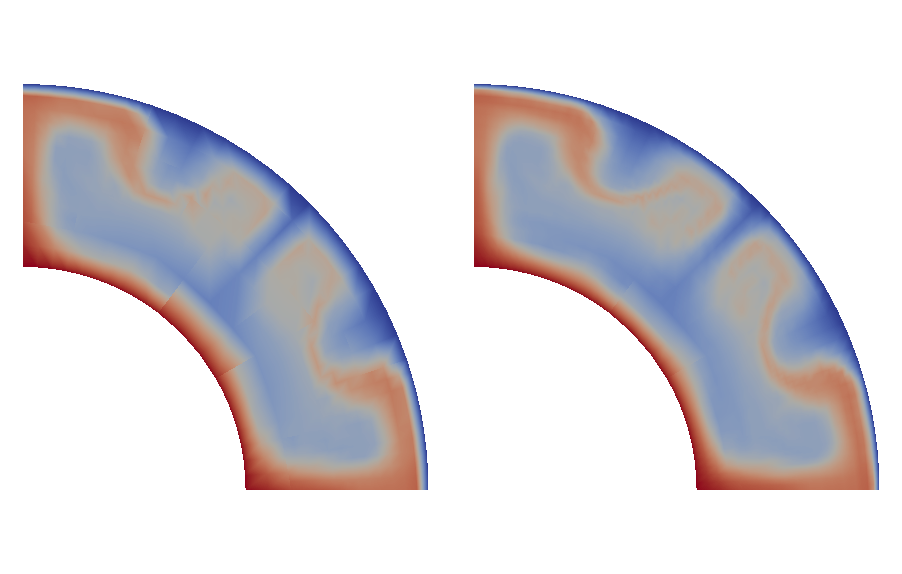
\includegraphics[width=0.5\textwidth]{viz/parameters/build-patches}\end{center}Here, the left picture shows one visualization cell per computational cell (i.e., the option is switched off), and the right picture shows the same simulation with the option switched on (which is the default). The images show the same data, demonstrating that interpolating the solution onto bilinear shape functions as is commonly done in visualizing data loses information.

Of course, activating this option also greatly increases the amount of data \aspect{} will write to disk: approximately by a factor of 4 in 2d, and a factor of 8 in 3d, when using quadratic elements for the velocity, and correspondingly more for even higher order elements.


{\it Possible values:} A boolean value (true or false)
\item {\it Parameter name:} {\tt List of output variables}
\phantomsection\label{parameters:Postprocess/Visualization/List of output variables}
\label{parameters:Postprocess/Visualization/List_20of_20output_20variables}


\index[prmindex]{List of output variables}
\index[prmindexfull]{Postprocess!Visualization!List of output variables}
{\it Value:} 


{\it Default:} 


{\it Description:} A comma separated list of visualization objects that should be run whenever writing graphical output. By default, the graphical output files will always contain the primary variables velocity, pressure, and temperature. However, one frequently wants to also visualize derived quantities, such as the thermodynamic phase that corresponds to a given temperature-pressure value, or the corresponding seismic wave speeds. The visualization objects do exactly this: they compute such derived quantities and place them into the output file. The current parameter is the place where you decide which of these additional output variables you want to have in your output file.

The following postprocessors are available:

`ISA rotation timescale': A visualization output object that generates output showing the timescale for the rotation of grains toward the infinite strain axis. Kaminski and Ribe (see \cite{Kaminski2002}) call this quantity $\tau_\text{ISA}$ and define it as $\tau_\text{ISA} \approx \frac{1}{\dot{\epsilon}}$ where $\dot{\epsilon}$ is the largest eigenvalue of the strain rate tensor. It can be used, along with the grain lag angle $\Theta$, to calculate the grain orientation lag parameter.

Physical units: \si{\second}.

`Vp anomaly': A visualization output object that generates output showing the percentage anomaly in the seismic compressional wave speed $V_p$ as a spatially variable function with one value per cell. This anomaly is either shown as a percentage anomaly relative to the reference profile given by adiabatic conditions (with the compositions given by the current composition, such that the reference could potentially change through time), or as a percentage change relative to the laterally averaged velocity at the depth of the cell. This velocity is calculated by linear interpolation between average values calculated within equally thick depth slices. The number of depth slices in the domain is user-defined. Typically, the best results will be obtained if the number of depth slices is balanced between being large enough to capture step changes in velocities, but small enough to maintain a reasonable number of evaluation points per slice. Bear in mind that lateral averaging subsamples the finite element mesh. Note that this plugin requires a material model that provides seismic velocities.

Physical units: None, the quantity being output is a fractional change provided as a percentage.

`Vs anomaly': A visualization output object that generates output showing the percentage anomaly in the seismic shear wave speed $V_s$ as a spatially variable function with one value per cell. This anomaly is either shown as a percentage anomaly relative to the reference profile given by adiabatic conditions (with the compositions given by the current composition, such that the reference could potentially change through time), or as a percentage change relative to the laterally averaged velocity at the depth of the cell. This velocity is calculated by linear interpolation between average values calculated within equally thick depth slices. The number of depth slices in the domain is user-defined. Typically, the best results will be obtained if the number of depth slices is balanced between being large enough to capture step changes in velocities, but small enough to maintain a reasonable number of evaluation points per slice. Bear in mind that lateral averaging subsamples the finite element mesh. Note that this plugin requires a material model that provides seismic velocities.

Physical units: None, the quantity being output is a fractional change provided as a percentage.

`adiabat': A visualization output object that generates adiabatic temperature, pressure, density, and density derivative (with regard to depth)as produced by the \texttt{AdiabaticConditions} class.

Physical units: \si{\kelvin}, \si{\pascal}, \si{\kilo\gram\per\meter\cubed\per\meter}, respectively, for the four components.

`artificial viscosity': A visualization output object that generates output showing the value of the artificial viscosity on each cell.

Physical units: \si{\watt\per\meter\per\kelvin}.

`artificial viscosity composition': A visualization output object that generates output showing the value of the artificial viscosity for a compositional field on each cell.

Physical units: \si{\meter\squared\per\second}.

`boundary indicators': A visualization output object that generates output about the used boundary indicators. In a loop over the active cells, if a cell lies at a domain boundary, the boundary indicator of the face along the boundary is requested. In case the cell does not lie along any domain boundary, the cell is assigned the value of the largest used boundary indicator plus one. When a cell is situated in one of the corners of the domain, multiple faces will have a boundary indicator. This postprocessor returns the value of the first face along a boundary that is encountered in a loop over all the faces.

Physical units: None.

`boundary strain rate residual': A visualization output object that generates output for the strain rate residual at the top surface. The residual is computed at each point at the surface as the difference between the strain rate invariant in the model and the input data, where the invariant is computed like in the 'strain rate' postprocessor. The user chooses the input data as ascii data files with coordinate columns and column corresponding to the surface strain rate norm.

Physical units: $\frac{1}{\text{s}}$ or $\frac{1}{\text{year}}$, depending on settings in the input file.

`boundary velocity residual': A visualization output object that generates output for the velocity residual at the top surface. The residual is computed at each point at the surface as the difference between the modeled velocities and the input data velocities for each vector component. The user has an option to choose the input data as ascii data files (e.g. GPS velocities) with columns in the same format as described for the 'ascii data' initial temperature plugin or a velocity field computed from the GPlates program as described in the gplates boundary velocity plugin.

Physical units: $\frac{\text{m}}{\text{s}}$ or $\frac{\text{m}}{\text{year}}$, depending on settings in the input file.

`compositional vector': A visualization output object that outputs vectors whose components are derived from compositional fields. Input parameters for this postprocessor are defined in section Postprocess/Visualization/Compositional fields as vectors.

Physical units: None.

`depth': A visualization output postprocessor that outputs the depth for all points inside the domain, as determined by the geometry model.

Physical units: \si{\meter}.

`dynamic topography': A visualization output object that generates output for the dynamic topography at the top and bottom of the model space. The approach to determine the dynamic topography requires us to compute the stress tensor and evaluate the component of it in the direction in which gravity acts. In other words, we compute $\sigma_{rr}={\hat g}^T(2 \eta \varepsilon(\mathbf u)-\frac 13 (\textrm{div}\;\mathbf u)I)\hat g - p_d$ where $\hat g = \mathbf g/\|\mathbf g\|$ is the direction of the gravity vector $\mathbf g$ and $p_d=p-p_a$ is the dynamic pressure computed by subtracting the adiabatic pressure $p_a$ from the total pressure $p$ computed as part of the Stokes solve. From this, the dynamic topography is computed using the formula $h=\frac{\sigma_{rr}}{(\mathbf g \cdot \mathbf n)  \rho}$ where $\rho$ is the density at the cell center. For the bottom surface we chose the convection that positive values are up (out) and negative values are in (down), analogous to the deformation of the upper surface. Note that this implementation takes the direction of gravity into account, which means that reversing the flow in backward advection calculations will not reverse the instantaneous topography because the reverse flow will be divided by the reverse surface gravity.

Strictly speaking, the dynamic topography is of course a quantity that is only of interest at the surface. However, we compute it everywhere to make things fit into the framework within which we produce data for visualization. You probably only want to visualize whatever data this postprocessor generates at the surface of your domain and simply ignore the rest of the data generated.

Alternatively, consider using the "surface dynamic topography" visualization postprocessor to only output the dynamic topography at the boundary of the domain.

Physical units: \si{\meter}.

`error indicator': A visualization output object that generates output showing the estimated error or other mesh refinement indicator as a spatially variable function with one value per cell.

Physical units: None. (Strictly speaking, errors have physical units of course, but because error \textit{indicators} can be computed from different solution components and other input, we consider error indicators unitless.)

`geoid': Visualization for the geoid solution. The geoid is given by the equivalent water column height due to a gravity perturbation. 

Physical units: \si{\meter}.

`grain lag angle': A visualization output object that generates output showing the angle between the ~infinite strain axis and the flow velocity. Kaminski and Ribe (see \cite{Kaminski2002}) call this quantity $\Theta$ and define it as $\Theta = \cos^{-1}(\hat{u}\cdot\hat{e})$  where $\hat{u}=\vec{u}/|{u}|$, $\vec{u}$ is the local flow velocity, and $\hat{e}$ is the local infinite strain axis, which we calculate as the first eigenvector of the 'left stretch' tensor. $\Theta$ can be used to calculate the grain orientation lag parameter.

Physical units: \si{\radian}.

`gravity': A visualization output object that outputs the gravity vector.

Physical units: \si {\meter\per\second\squared} .

`heat flux map': A visualization output object that generates output for the heat flux density across the top and bottom boundary in outward direction. The heat flux is computed as sum of advective heat flux and conductive heat flux through Neumann boundaries, both computed as integral over the boundary area, and conductive heat flux through Dirichlet boundaries, which is computed using the consistent boundary flux method as described in ``Gresho, Lee, Sani, Maslanik, Eaton (1987). The consistent Galerkin FEM for computing derived boundary quantities in thermal and or fluids problems. International Journal for Numerical Methods in Fluids, 7(4), 371-394.'' If only conductive heat flux through Dirichlet boundaries is of interest, the postprocessor can produce output of higher resolution by evaluating the CBF solution vector point-wise instead of computing cell-wise averaged values.

Physical units: \si{\watt\per\meter\squared}.

`heating': A visualization output object that generates output for all the heating terms used in the energy equation.

Physical units: \si{\watt\per\cubic\meter}.

`material properties': A visualization output object that generates output for the material properties given by the material model. The current postprocessor allows to output a (potentially large) subset of all of the information provided by material models at once, with just a single material model evaluation per output point. Although individual properties can still be listed in the ``List of output variables'', this visualization plugin is called internally to avoid duplicated evaluations of the material model. 

In almost all places inside \aspect{}, the program can use ``averaged'' material properties, for example for the assembly of matrices and right hand side vectors. To accurately reflect the material parameters used internally, this visualization postprocessor averages in the same way as is used to do the assembly, and consequently the graphical output will reflect not pointwise properties, but averaged properties.

Physical units: Various.

`maximum horizontal compressive stress': A plugin that computes the direction and magnitude of the maximum horizontal component of the compressive stress as a vector field. The direction of this vector can often be used to visualize the principal mode of deformation (e.g., at normal faults or extensional margins) and can be correlated with seismic anisotropy. Recall that the \textit{compressive} stress is simply the negative stress, $\sigma_c=-\sigma=-\left[     2\eta (\varepsilon(\mathbf u)             - \frac 13 (\nabla \cdot \mathbf u) I)     + pI\right]$.

Following \cite{LundTownend07}, we define the maximum horizontal stress direction as that \textit{horizontal} direction $\mathbf n$ that maximizes $\mathbf n^T \sigma_c \mathbf n$. We call a vector \textit{horizontal} if it is perpendicular to the gravity vector $\mathbf g$.

In two space dimensions, $\mathbf n$ is simply a vector that is horizontal (we choose one of the two possible choices). This direction is then scaled by the size of the horizontal stress in this direction, i.e., the plugin outputs the vector $\mathbf w = (\mathbf n^T \sigma_c \mathbf n) \; \mathbf n$.

In three space dimensions, given two horizontal, perpendicular, unit length, but otherwise arbitrarily chosen vectors $\mathbf u,\mathbf v$, we can express $\mathbf n = (\cos \alpha)\mathbf u + (\sin\alpha)\mathbf v$ where $\alpha$ maximizes the expression \begin{align*}  f(\alpha) = \mathbf n^T \sigma_c \mathbf n  = (\mathbf u^T \sigma_c \mathbf u)(\cos\alpha)^2    +2(\mathbf u^T \sigma_c \mathbf v)(\cos\alpha)(\sin\alpha)    +(\mathbf v^T \sigma_c \mathbf v)(\sin\alpha)^2.\end{align*}

The maximum of $f(\alpha)$ is attained where $f'(\alpha)=0$. Evaluating the derivative and using trigonometric identities, one finds that $\alpha$ has to satisfy the equation \begin{align*}  \tan(2\alpha) = \frac{2.0\mathbf u^T \sigma_c \mathbf v}                          {\mathbf u^T \sigma_c \mathbf u                            - \mathbf v^T \sigma_c \mathbf v}.\end{align*}Since the transform $\alpha\mapsto\alpha+\pi$ flips the direction of $\mathbf n$, we only need to seek a solution to this equation in the interval $\alpha\in[0,\pi)$. These are given by $\alpha_1=\frac 12 \arctan \frac{\mathbf u^T \sigma_c \mathbf v}{\mathbf u^T \sigma_c \mathbf u - \mathbf v^T \sigma_c \mathbf v}$ and $\alpha_2=\alpha_1+\frac{\pi}{2}$, one of which will correspond to a minimum and the other to a maximum of $f(\alpha)$. One checks the sign of $f''(\alpha)=-2(\mathbf u^T \sigma_c \mathbf u - \mathbf v^T \sigma_c \mathbf v)\cos(2\alpha) - 2 (\mathbf u^T \sigma_c \mathbf v) \sin(2\alpha)$ for each of these to determine the $\alpha$ that maximizes $f(\alpha)$, and from this immediately arrives at the correct form for the maximum horizontal stress $\mathbf n$.

The description above computes a 3d \textit{direction} vector $\mathbf n$. If one were to scale this vector the same way as done in 2d, i.e., with the magnitude of the stress in this direction, one will typically get vectors whose length is principally determined by the hydrostatic pressure at a given location simply because the hydrostatic pressure is the largest component of the overall stress. On the other hand, the hydrostatic pressure does not determine any principal direction because it is an isotropic, anti-compressive force. As a consequence, there are often points in simulations (e.g., at the center of convection rolls) where the stress has no dominant horizontal direction, and the algorithm above will then in essence choose a random direction because the stress is approximately equal in all horizontal directions. If one scaled the output by the magnitude of the stress in this direction (i.e., approximately equal to the hydrostatic pressure at this point), one would get randomly oriented vectors at these locations with significant lengths.

To avoid this problem, we scale the maximal horizontal compressive stress direction $\mathbf n$ by the \textit{difference} between the stress in the maximal and minimal horizontal stress directions. In other words, let $\mathbf n_\perp=(\sin \alpha)\mathbf u - (\cos\alpha)\mathbf v$ be the horizontal direction perpendicular to $\mathbf n$, then this plugin outputs the vector quantity $\mathbf w = (\mathbf n^T \sigma_c \mathbf n                -\mathbf n^T_\perp \sigma_c \mathbf n_\perp)               \; \mathbf n$. In other words, the length of the vector produced indicates \textit{how dominant} the direction of maximal horizontal compressive strength is.

Fig.~\ref{fig:max-horizontal-compressive-stress} shows a simple example for this kind of visualization in 3d.

\begin{figure}  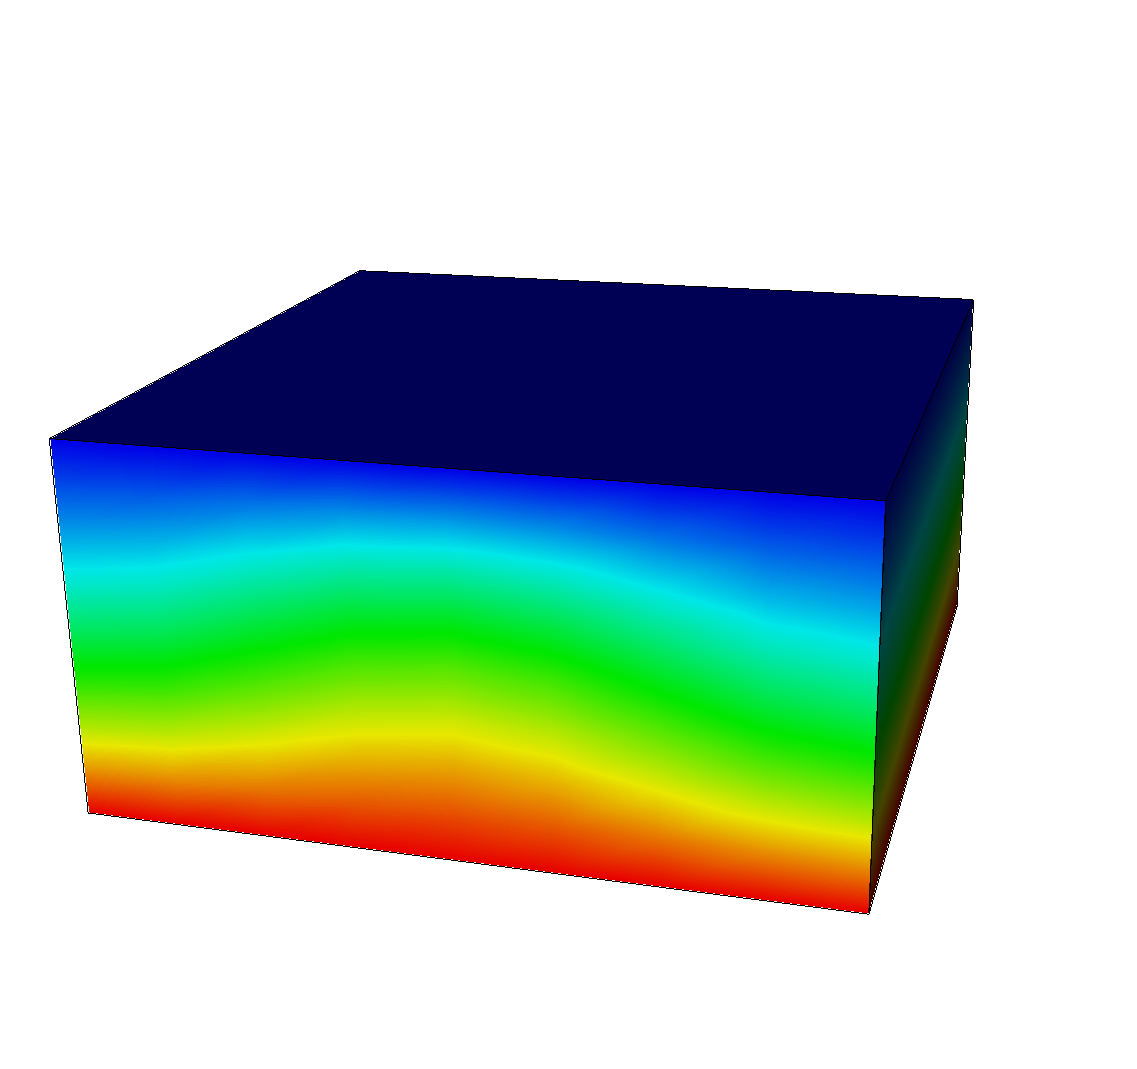
\includegraphics[width=0.3\textwidth]    {viz/plugins/maximum_horizontal_compressive_stress/temperature.png}  \hfill  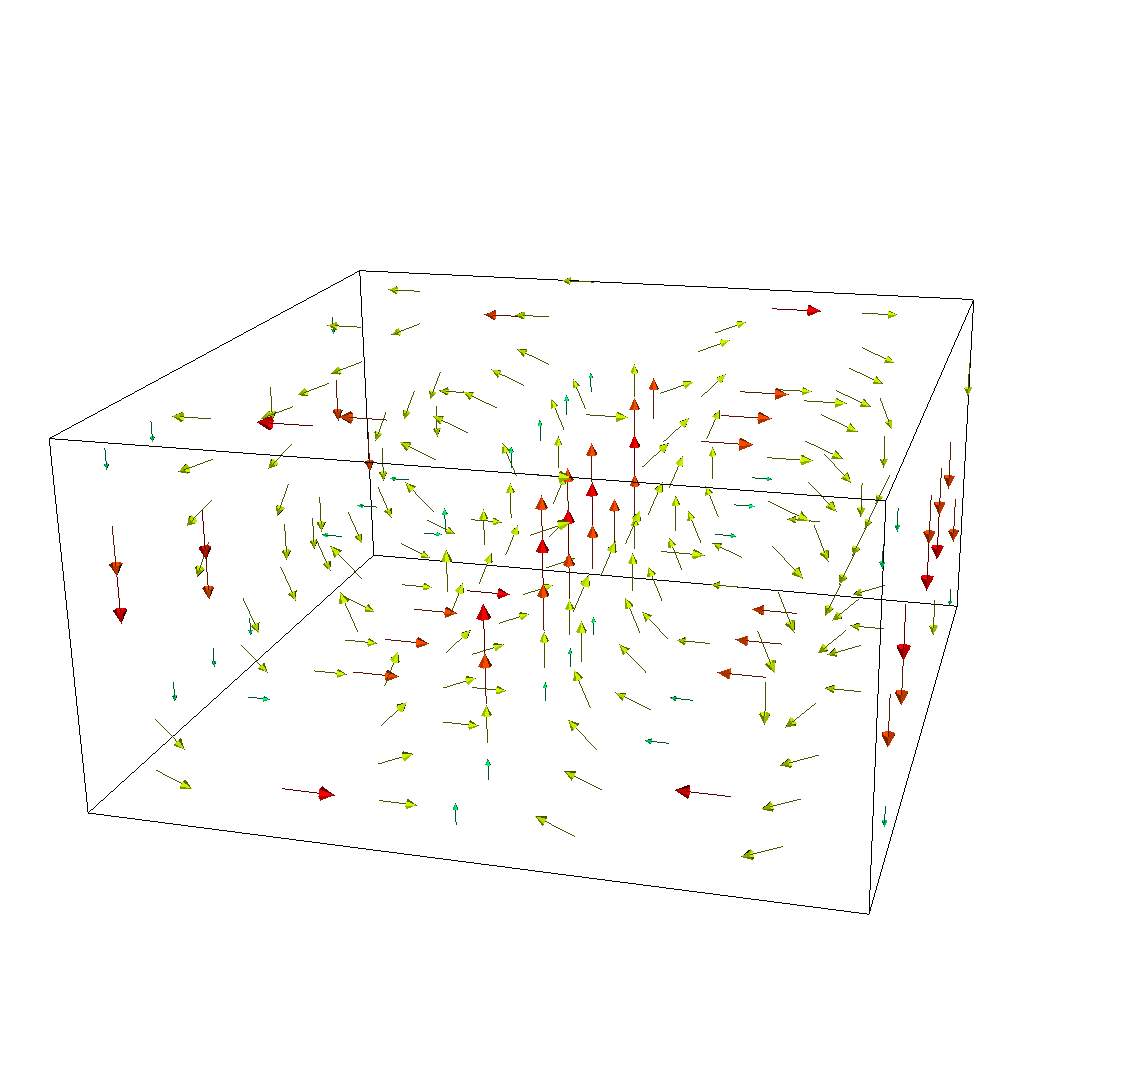
\includegraphics[width=0.3\textwidth]    {viz/plugins/maximum_horizontal_compressive_stress/velocity.png}  \hfill  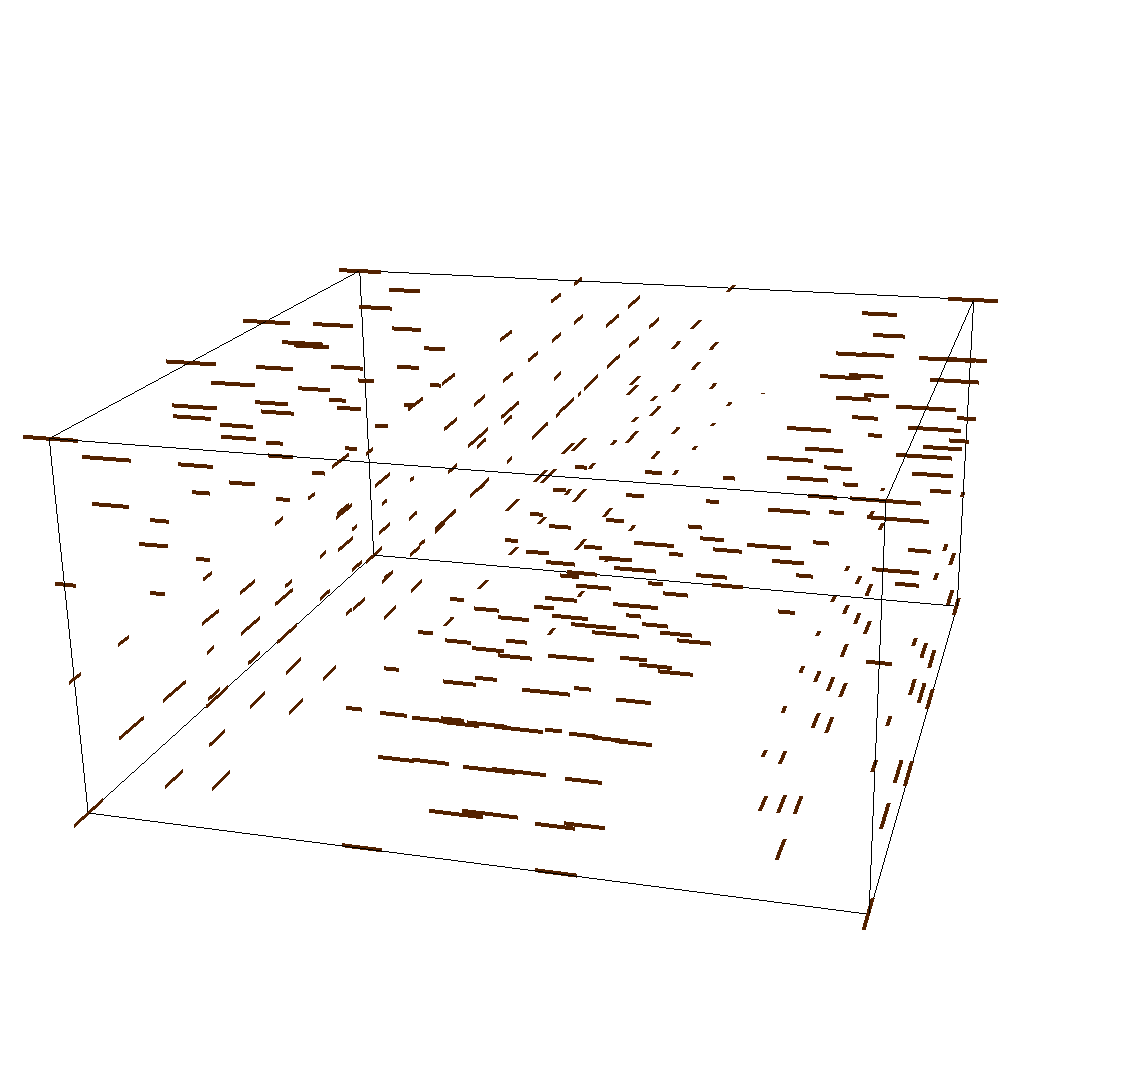
\includegraphics[width=0.3\textwidth]    {viz/plugins/maximum_horizontal_compressive_stress/horizontal-stress.png}  \caption{\it Illustration of the `maximum horizontal     compressive stress' visualization plugin. The left     figure shows a ridge-like temperature anomaly. Together     with no-slip boundary along all six boundaries, this     results in two convection rolls (center). The maximal     horizontal compressive strength at the bottom center     of the domain is perpendicular to the ridge because     the flow comes together there from the left and right,     yielding a compressive force in left-right direction.     At the top of the model, the flow separates outward,     leading to a \textit{negative} compressive stress     in left-right direction; because there is no flow     in front-back direction, the compressive strength     in front-back direction is zero, making the along-ridge     direction the dominant one. At the center of the     convection rolls, both horizontal directions yield     the same stress; the plugin therefore chooses an     essentially arbitrary horizontal vector, but then     uses a zero magnitude given that the difference     between the maximal and minimal horizontal stress     is zero at these points.}  \label{fig:max-horizontal-compressive-stress}\end{figure}

Physical units: \si{\pascal}.

`melt fraction': A visualization output object that generates output for the melt fraction at the temperature and pressure of the current point. If the material model computes a melt fraction, this is the quantity that will be visualized. Otherwise, a specific parametrization for batch melting (as described in the following) will be used. It does not take into account latent heat. If there are no compositional fields, or no fields called 'pyroxenite',  this postprocessor will visualize the melt fraction of peridotite (calculated using the anhydrous model of Katz, 2003). If there is a compositional field called 'pyroxenite', the postprocessor assumes that this compositional field is the content of pyroxenite, and will visualize the melt fraction for a mixture of peridotite and pyroxenite (using the melting model of Sobolev, 2011 for pyroxenite). All the parameters that were used in these calculations can be changed in the input file, the most relevant maybe being the mass fraction of Cpx in peridotite in the Katz melting model (Mass fraction cpx), which right now has a default of 15\%. The corresponding $p$-$T$-diagrams can be generated by running the tests melt\_postprocessor\_peridotite and melt\_postprocessor\_pyroxenite.

Physical units: None.

`melt material properties': A visualization output object that generates output for melt related properties of the material model. Note that this postprocessor always outputs the compaction pressure, but can output a large range of additional properties, as selected in the ``List of properties'' parameter.

Physical units: Various, depending on what is being output.

`named additional outputs': Some material models can compute quantities other than those that typically appear in the equations that \aspect{} solves (such as the viscosity, density, etc). Examples of quantities material models may be able to compute are seismic velocities, or other quantities that can be derived from the state variables and the material coefficients such as the stress or stress anisotropies. These quantities are generically referred to as `named outputs' because they are given an explicit name different from the usual outputs of material models.

This visualization postprocessor outputs whatever quantities the material model can compute. What quantities these are is specific to the material model in use for a simulation, and for many models in fact does not contain any named outputs at all.

Physical units: Various, depending on what is being output.

`nonadiabatic pressure': A visualization output object that generates output for the non-adiabatic component of the pressure.

The variable that is outputted this way is computed by taking the pressure at each point and subtracting from it the adiabatic pressure computed at the beginning of the simulation. Because the adiabatic pressure is one way of defining a static pressure background field, what this visualization postprocessor therefore produces is \textit{one} way to compute a \textit{dynamic pressure}. There are, however, other ways as well, depending on the choice of the ``background pressure''.

Physical units: \si{\pascal}.

`nonadiabatic temperature': A visualization output object that generates output for the non-adiabatic component of the temperature.

Physical units: \si{\kelvin}.

`particle count': A visualization output object that generates output about the number of particles per cell.

Physical units: None.

`partition': A visualization output object that generates output for the parallel partition that every cell of the mesh is associated with.

Physical units: None.

`principal stress': A visualization output object that outputs the principal stress values and directions, i.e., the eigenvalues and eigenvectors of the stress tensor. The postprocessor can either operate on the full stress tensor or only on the deviatoric stress tensor, depending on what run-time parameters are set.

Physical units: \si{\pascal}.

`shear stress': A visualization output object that generates output for the 3 (in 2d) or 6 (in 3d) components of the shear stress tensor, i.e., for the components of the tensor $-2\eta\varepsilon(\mathbf u)$ in the incompressible case and $-2\eta\left[\varepsilon(\mathbf u)-\tfrac 13(\textrm{tr}\;\varepsilon(\mathbf u))\mathbf I\right]$ in the compressible case. If elasticity is used, the elastic contribution is being accounted for. The shear stress differs from the full stress tensor by the absence of the pressure. Note that the convention of positive compressive stress is followed.

Physical units: \si{\pascal}.

`spd factor': A visualization output object that generates output for the spd factor. The spd factor is a factor which scales a part of the Jacobian used for the Newton solver to make sure that the Jacobian remains positive definite.

Physical units: None.

`spherical velocity components': A visualization output object that outputs the polar coordinates components $v_r$ and $v_\phi$ of the velocity field in 2D and the spherical coordinates components $v_r$, $v_{\phi}$ and $v_{\theta}$ of the velocity field in 3D.

Physical units: $\frac{\text{m}}{\text{s}}$ or $\frac{\text{m}}{\text{year}}$, depending on settings in the input file.

`strain rate': A visualization output object that generates output for the norm of the strain rate, i.e., for the quantity $\sqrt{\varepsilon(\mathbf u):\varepsilon(\mathbf u)}$ in the incompressible case and $\sqrt{[\varepsilon(\mathbf u)-\tfrac 13(\textrm{tr}\;\varepsilon(\mathbf u))\mathbf I]:[\varepsilon(\mathbf u)-\tfrac 13(\textrm{tr}\;\varepsilon(\mathbf u))\mathbf I]}$ in the compressible case.

Physical units: \si{\per\second}.

`strain rate tensor': A visualization output object that generates output for the 4 (in 2d) or 9 (in 3d) components of the strain rate tensor, i.e., for the components of the tensor $\varepsilon(\mathbf u)$ in the incompressible case and $\varepsilon(\mathbf u)-\tfrac 13(\textrm{tr}\;\varepsilon(\mathbf u))\mathbf I$ in the compressible case.

Physical units: \si{\per\second}.

`stress': A visualization output object that generates output for the 3 (in 2d) or 6 (in 3d) components of the stress tensor, i.e., for the components of the tensor $-2\eta\varepsilon(\mathbf u)+pI$ in the incompressible case and $-2\eta\left[\varepsilon(\mathbf u)-\tfrac 13(\textrm{tr}\;\varepsilon(\mathbf u))\mathbf I\right]+pI$ in the compressible case. If elasticity is used, the elastic contribution is being accounted for. Note that the convention of positive compressive stress is followed.

Physical units: \si{\pascal}.

`stress second invariant': A visualization output object that outputs the second moment invariant of the deviatoric stress tensor.

Physical units: \si{\pascal}.

`surface dynamic topography': A visualization output object that generates output for the dynamic topography at the top and bottom of the model space. The approach to determine the dynamic topography requires us to compute the stress tensor and evaluate the component of it in the direction in which gravity acts. In other words, we compute $\sigma_{rr}={\hat g}^T(2 \eta \varepsilon(\mathbf u)-\frac 13 (\textrm{div}\;\mathbf u)I)\hat g - p_d$ where $\hat g = \mathbf g/\|\mathbf g\|$ is the direction of the gravity vector $\mathbf g$ and $p_d=p-p_a$ is the dynamic pressure computed by subtracting the adiabatic pressure $p_a$ from the total pressure $p$ computed as part of the Stokes solve. From this, the dynamic topography is computed using the formula $h=\frac{\sigma_{rr}}{(\mathbf g \cdot \mathbf n)  \rho}$ where $\rho$ is the density at the cell center. For the bottom surface we chose the convection that positive values are up (out) and negative values are in (down), analogous to the deformation of the upper surface. Note that this implementation takes the direction of gravity into account, which means that reversing the flow in backward advection calculations will not reverse the instantaneous topography because the reverse flow will be divided by the reverse surface gravity.

In contrast to the `dynamic topography' visualization postprocessor, this plugin really only evaluates the dynamic topography at faces of cells that are adjacent to `bottom' and `top' boundaries, and only outputs information on the surface of the domain, rather than padding the information with zeros in the interior of the domain.

Physical units: \si{\meter}.

`surface stress': A visualization output object that generates output on the surface of the domain for the 3 (in 2d) or 6 (in 3d) components of the stress tensor, i.e., for the components of the tensor $-2\eta\varepsilon(\mathbf u)+pI$ in the incompressible case and $-2\eta\left[\varepsilon(\mathbf u)-\tfrac 13(\textrm{tr}\;\varepsilon(\mathbf u))\mathbf I\right]+pI$ in the compressible case. If elasticity is included, its contribution is accounted for. Note that the convention of positive compressive stress is followed.

Physical units: \si{\pascal}.

`temperature anomaly': A visualization output postprocessor that outputs the temperature minus the depth-average of the temperature.The average temperature is calculated using the lateral averaging function from the ``depth average'' postprocessor and interpolated linearly between the layers specified through ``Number of depth slices''.

Physical units: \si{\kelvin}.

`vertical heat flux': A visualization output object that generates output for the heat flux in the vertical direction, which is the sum of the advective and the conductive heat flux, with the sign convention of positive flux upwards.

Physical units: \si{\watt\per\square\meter}.

`volume of fluid values': A visualization output object that outputs the volume fraction and optionally a level set field and the interface normal vectors of volume of fluid fields.

Physical units: None.

`volumetric strain rate': A visualization output object that generates output for the volumetric strain rate, i.e., for the quantity $\nabla\cdot\mathbf u = \textrm{div}\; \mathbf u = \textrm{trace}\; \varepsilon(\mathbf u)$. This should be zero (in some average sense) in incompressible convection models, but can be non-zero in compressible models and models with melt transport.

Physical units: \si{\per\second}.


{\it Possible values:} A comma-separated list of any of ISA rotation timescale, Vp anomaly, Vs anomaly, adiabat, artificial viscosity, artificial viscosity composition, boundary indicators, boundary strain rate residual, boundary velocity residual, compositional vector, depth, dynamic topography, error indicator, geoid, grain lag angle, gravity, heat flux map, heating, material properties, maximum horizontal compressive stress, melt fraction, melt material properties, named additional outputs, nonadiabatic pressure, nonadiabatic temperature, particle count, partition, principal stress, shear stress, spd factor, spherical velocity components, strain rate, strain rate tensor, stress, stress second invariant, surface dynamic topography, surface stress, temperature anomaly, vertical heat flux, volume of fluid values, volumetric strain rate, density, specific heat, thermal conductivity, thermal diffusivity, thermal expansivity, viscosity
\item {\it Parameter name:} {\tt Number of grouped files}
\phantomsection\label{parameters:Postprocess/Visualization/Number of grouped files}
\label{parameters:Postprocess/Visualization/Number_20of_20grouped_20files}


\index[prmindex]{Number of grouped files}
\index[prmindexfull]{Postprocess!Visualization!Number of grouped files}
{\it Value:} 16


{\it Default:} 16


{\it Description:} VTU file output supports grouping files from several CPUs into a given number of files using MPI I/O when writing on a parallel filesystem. Select 0 for no grouping. This will disable parallel file output and instead write one file per processor. A value of 1 will generate one big file containing the whole solution, while a larger value will create that many files (at most as many as there are MPI ranks).


{\it Possible values:} An integer $n$ such that $0\leq n \leq 2147483647$
\item {\it Parameter name:} {\tt Output format}
\phantomsection\label{parameters:Postprocess/Visualization/Output format}
\label{parameters:Postprocess/Visualization/Output_20format}


\index[prmindex]{Output format}
\index[prmindexfull]{Postprocess!Visualization!Output format}
{\it Value:} vtu


{\it Default:} vtu


{\it Description:} The file format to be used for graphical output. The list of possible output formats that can be given here is documented in the appendix of the manual where the current parameter is described.


{\it Possible values:} Any one of none, dx, ucd, gnuplot, povray, eps, gmv, tecplot, tecplot\_binary, vtk, vtu, hdf5, svg, deal.II intermediate
\item {\it Parameter name:} {\tt Output mesh velocity}
\phantomsection\label{parameters:Postprocess/Visualization/Output mesh velocity}
\label{parameters:Postprocess/Visualization/Output_20mesh_20velocity}


\index[prmindex]{Output mesh velocity}
\index[prmindexfull]{Postprocess!Visualization!Output mesh velocity}
{\it Value:} false


{\it Default:} false


{\it Description:} For computations with deforming meshes, ASPECT uses an Arbitrary-Lagrangian-Eulerian formulation to handle deforming the domain, so the mesh has its own velocity field.  This may be written as an output field by setting this parameter to true.


{\it Possible values:} A boolean value (true or false)
\item {\it Parameter name:} {\tt Point-wise stress and strain}
\phantomsection\label{parameters:Postprocess/Visualization/Point_2dwise stress and strain}
\label{parameters:Postprocess/Visualization/Point_2dwise_20stress_20and_20strain}


\index[prmindex]{Point-wise stress and strain}
\index[prmindexfull]{Postprocess!Visualization!Point-wise stress and strain}
{\it Value:} false


{\it Default:} false


{\it Description:} If set to true, quantities related to stress and strain are computed in each vertex. Otherwise, an average per cell is computed.


{\it Possible values:} A boolean value (true or false)
\item {\it Parameter name:} {\tt Temporary output location}
\phantomsection\label{parameters:Postprocess/Visualization/Temporary output location}
\label{parameters:Postprocess/Visualization/Temporary_20output_20location}


\index[prmindex]{Temporary output location}
\index[prmindexfull]{Postprocess!Visualization!Temporary output location}
{\it Value:} 


{\it Default:} 


{\it Description:} On large clusters it can be advantageous to first write the output to a temporary file on a local file system and later move this file to a network file system. If this variable is set to a non-empty string it will be interpreted as a temporary storage location.


{\it Possible values:} Any string
\item {\it Parameter name:} {\tt Time between graphical output}
\phantomsection\label{parameters:Postprocess/Visualization/Time between graphical output}
\label{parameters:Postprocess/Visualization/Time_20between_20graphical_20output}


\index[prmindex]{Time between graphical output}
\index[prmindexfull]{Postprocess!Visualization!Time between graphical output}
{\it Value:} 1e8


{\it Default:} 1e8


{\it Description:} The time interval between each generation of graphical output files. A value of zero indicates that output should be generated in each time step. Units: years if the 'Use years in output instead of seconds' parameter is set; seconds otherwise.


{\it Possible values:} A floating point number $v$ such that $0 \leq v \leq \text{MAX\_DOUBLE}$
\item {\it Parameter name:} {\tt Time steps between graphical output}
\phantomsection\label{parameters:Postprocess/Visualization/Time steps between graphical output}
\label{parameters:Postprocess/Visualization/Time_20steps_20between_20graphical_20output}


\index[prmindex]{Time steps between graphical output}
\index[prmindexfull]{Postprocess!Visualization!Time steps between graphical output}
{\it Value:} 2147483647


{\it Default:} 2147483647


{\it Description:} The maximum number of time steps between each generation of graphical output files.


{\it Possible values:} An integer $n$ such that $0\leq n \leq 2147483647$
\item {\it Parameter name:} {\tt Write higher order output}
\phantomsection\label{parameters:Postprocess/Visualization/Write higher order output}
\label{parameters:Postprocess/Visualization/Write_20higher_20order_20output}


\index[prmindex]{Write higher order output}
\index[prmindexfull]{Postprocess!Visualization!Write higher order output}
{\it Value:} false


{\it Default:} false


{\it Description:} deal.II offers the possibility to write vtu files with higher order representations of the output data. This means each cell will correctly show the higher order representation of the output data instead of the linear interpolation between vertices that ParaView and VisIt usually show. Note that activating this option is safe and recommended, but requires that (i) ``Output format'' is set to ``vtu'', (ii) ``Interpolate output'' is set to true, (iii) you use a sufficiently new version of Paraview or VisIt to read the files (Paraview version 5.5 or newer, and VisIt version to be determined), and (iv) you use deal.II version 9.1.0 or newer. 
The effect of using this option can be seen in the following picture:

\begin{center}  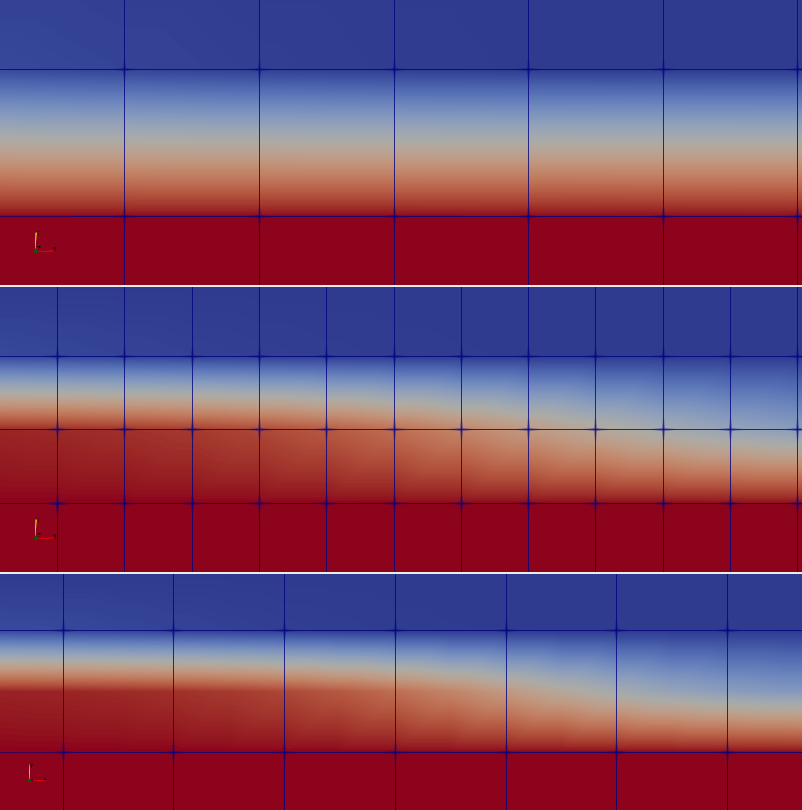
\includegraphics[width=0.5\textwidth]{viz/parameters/higher-order-output}\end{center}The top figure shows the plain output without interpolation or higher order output. The middle figure shows output that was interpolated as discussed for the ``Interpolate output'' option. The bottom panel shows higher order output that achieves better accuracy than the interpolated output at a lower memory cost.


{\it Possible values:} A boolean value (true or false)
\item {\it Parameter name:} {\tt Write in background thread}
\phantomsection\label{parameters:Postprocess/Visualization/Write in background thread}
\label{parameters:Postprocess/Visualization/Write_20in_20background_20thread}


\index[prmindex]{Write in background thread}
\index[prmindexfull]{Postprocess!Visualization!Write in background thread}
{\it Value:} false


{\it Default:} false


{\it Description:} File operations can potentially take a long time, blocking the progress of the rest of the model run. Setting this variable to `true' moves this process into a background thread, while the rest of the model continues.


{\it Possible values:} A boolean value (true or false)
\end{itemize}



\subsection{Parameters in section \tt Postprocess/Visualization/Artificial viscosity composition}
\label{parameters:Postprocess/Visualization/Artificial_20viscosity_20composition}

\begin{itemize}
\item {\it Parameter name:} {\tt Name of compositional field}
\phantomsection\label{parameters:Postprocess/Visualization/Artificial viscosity composition/Name of compositional field}
\label{parameters:Postprocess/Visualization/Artificial_20viscosity_20composition/Name_20of_20compositional_20field}


\index[prmindex]{Name of compositional field}
\index[prmindexfull]{Postprocess!Visualization!Artificial viscosity composition/Name of compositional field}
{\it Value:} 


{\it Default:} 


{\it Description:} The name of the compositional field whose output should be visualized. 


{\it Possible values:} Any string
\end{itemize}

\subsection{Parameters in section \tt Postprocess/Visualization/Compositional fields as vectors}
\label{parameters:Postprocess/Visualization/Compositional_20fields_20as_20vectors}

\begin{itemize}
\item {\it Parameter name:} {\tt Names of fields}
\phantomsection\label{parameters:Postprocess/Visualization/Compositional fields as vectors/Names of fields}
\label{parameters:Postprocess/Visualization/Compositional_20fields_20as_20vectors/Names_20of_20fields}


\index[prmindex]{Names of fields}
\index[prmindexfull]{Postprocess!Visualization!Compositional fields as vectors/Names of fields}
{\it Value:} 


{\it Default:} 


{\it Description:} A list of sets of compositional fields which should be output as vectors. Sets are separated from each other by semicolons and vector components within each set are separated by commas (e.g. $vec1_x$, $vec1_y$ ; $vec2_x$, $vec2_y$) where each name must be a defined named compositional field. If only one name is given in a set, it is interpreted as the first in a sequence of dim consecutive compositional fields.


{\it Possible values:} Any string
\item {\it Parameter name:} {\tt Names of vectors}
\phantomsection\label{parameters:Postprocess/Visualization/Compositional fields as vectors/Names of vectors}
\label{parameters:Postprocess/Visualization/Compositional_20fields_20as_20vectors/Names_20of_20vectors}


\index[prmindex]{Names of vectors}
\index[prmindexfull]{Postprocess!Visualization!Compositional fields as vectors/Names of vectors}
{\it Value:} 


{\it Default:} 


{\it Description:} Names of vectors as they will appear in the output.


{\it Possible values:} A list of 0 to 4294967295 elements where each element is [Any string]
\end{itemize}

\subsection{Parameters in section \tt Postprocess/Visualization/Heat flux map}
\label{parameters:Postprocess/Visualization/Heat_20flux_20map}

\begin{itemize}
\item {\it Parameter name:} {\tt Output point wise heat flux}
\phantomsection\label{parameters:Postprocess/Visualization/Heat flux map/Output point wise heat flux}
\label{parameters:Postprocess/Visualization/Heat_20flux_20map/Output_20point_20wise_20heat_20flux}


\index[prmindex]{Output point wise heat flux}
\index[prmindexfull]{Postprocess!Visualization!Heat flux map/Output point wise heat flux}
{\it Value:} false


{\it Default:} false


{\it Description:} A boolean flag that controls whether to output the heat flux map as a point wise value, or as a cell-wise averaged value. The point wise output is more accurate, but it currently omits prescribed heat flux values at boundaries and advective heat flux that is caused by velocities non-tangential to boundaries. If you do not use these two features it is recommended to switch this setting on to benefit from the increased output resolution.


{\it Possible values:} A boolean value (true or false)
\end{itemize}

\subsection{Parameters in section \tt Postprocess/Visualization/Material properties}
\label{parameters:Postprocess/Visualization/Material_20properties}

\begin{itemize}
\item {\it Parameter name:} {\tt List of material properties}
\phantomsection\label{parameters:Postprocess/Visualization/Material properties/List of material properties}
\label{parameters:Postprocess/Visualization/Material_20properties/List_20of_20material_20properties}


\index[prmindex]{List of material properties}
\index[prmindexfull]{Postprocess!Visualization!Material properties/List of material properties}
{\it Value:} density,thermal expansivity,specific heat,viscosity


{\it Default:} density,thermal expansivity,specific heat,viscosity


{\it Description:} A comma separated list of material properties that should be written whenever writing graphical output. By default, the material properties will always contain the density, thermal expansivity, specific heat and viscosity. The following material properties are available:

viscosity|density|thermal expansivity|specific heat|thermal conductivity|thermal diffusivity|compressibility|entropy derivative temperature|entropy derivative pressure|reaction terms|melt fraction


{\it Possible values:} A comma-separated list of any of viscosity, density, thermal expansivity, specific heat, thermal conductivity, thermal diffusivity, compressibility, entropy derivative temperature, entropy derivative pressure, reaction terms, melt fraction
\end{itemize}

\subsection{Parameters in section \tt Postprocess/Visualization/Melt fraction}
\label{parameters:Postprocess/Visualization/Melt_20fraction}

\begin{itemize}
\item {\it Parameter name:} {\tt A1}
\phantomsection\label{parameters:Postprocess/Visualization/Melt fraction/A1}
\label{parameters:Postprocess/Visualization/Melt_20fraction/A1}


\index[prmindex]{A1}
\index[prmindexfull]{Postprocess!Visualization!Melt fraction/A1}
{\it Value:} 1085.7


{\it Default:} 1085.7


{\it Description:} Constant parameter in the quadratic function that approximates the solidus of peridotite. Units: \si{\degreeCelsius}.


{\it Possible values:} A floating point number $v$ such that $-\text{MAX\_DOUBLE} \leq v \leq \text{MAX\_DOUBLE}$
\item {\it Parameter name:} {\tt A2}
\phantomsection\label{parameters:Postprocess/Visualization/Melt fraction/A2}
\label{parameters:Postprocess/Visualization/Melt_20fraction/A2}


\index[prmindex]{A2}
\index[prmindexfull]{Postprocess!Visualization!Melt fraction/A2}
{\it Value:} 1.329e-7


{\it Default:} 1.329e-7


{\it Description:} Prefactor of the linear pressure term in the quadratic function that approximates the solidus of peridotite. \si{\degreeCelsius\per\pascal}.


{\it Possible values:} A floating point number $v$ such that $-\text{MAX\_DOUBLE} \leq v \leq \text{MAX\_DOUBLE}$
\item {\it Parameter name:} {\tt A3}
\phantomsection\label{parameters:Postprocess/Visualization/Melt fraction/A3}
\label{parameters:Postprocess/Visualization/Melt_20fraction/A3}


\index[prmindex]{A3}
\index[prmindexfull]{Postprocess!Visualization!Melt fraction/A3}
{\it Value:} -5.1e-18


{\it Default:} -5.1e-18


{\it Description:} Prefactor of the quadratic pressure term in the quadratic function that approximates the solidus of peridotite. \si{\degreeCelsius\per\pascal\squared}.


{\it Possible values:} A floating point number $v$ such that $-\text{MAX\_DOUBLE} \leq v \leq \text{MAX\_DOUBLE}$
\item {\it Parameter name:} {\tt B1}
\phantomsection\label{parameters:Postprocess/Visualization/Melt fraction/B1}
\label{parameters:Postprocess/Visualization/Melt_20fraction/B1}


\index[prmindex]{B1}
\index[prmindexfull]{Postprocess!Visualization!Melt fraction/B1}
{\it Value:} 1475.0


{\it Default:} 1475.0


{\it Description:} Constant parameter in the quadratic function that approximates the lherzolite liquidus used for calculating the fraction of peridotite-derived melt. Units: \si{\degreeCelsius}.


{\it Possible values:} A floating point number $v$ such that $-\text{MAX\_DOUBLE} \leq v \leq \text{MAX\_DOUBLE}$
\item {\it Parameter name:} {\tt B2}
\phantomsection\label{parameters:Postprocess/Visualization/Melt fraction/B2}
\label{parameters:Postprocess/Visualization/Melt_20fraction/B2}


\index[prmindex]{B2}
\index[prmindexfull]{Postprocess!Visualization!Melt fraction/B2}
{\it Value:} 8.0e-8


{\it Default:} 8.0e-8


{\it Description:} Prefactor of the linear pressure term in the quadratic function that approximates the  lherzolite liquidus used for calculating the fraction of peridotite-derived melt. \si{\degreeCelsius\per\pascal}.


{\it Possible values:} A floating point number $v$ such that $-\text{MAX\_DOUBLE} \leq v \leq \text{MAX\_DOUBLE}$
\item {\it Parameter name:} {\tt B3}
\phantomsection\label{parameters:Postprocess/Visualization/Melt fraction/B3}
\label{parameters:Postprocess/Visualization/Melt_20fraction/B3}


\index[prmindex]{B3}
\index[prmindexfull]{Postprocess!Visualization!Melt fraction/B3}
{\it Value:} -3.2e-18


{\it Default:} -3.2e-18


{\it Description:} Prefactor of the quadratic pressure term in the quadratic function that approximates the  lherzolite liquidus used for calculating the fraction of peridotite-derived melt. \si{\degreeCelsius\per\pascal\squared}.


{\it Possible values:} A floating point number $v$ such that $-\text{MAX\_DOUBLE} \leq v \leq \text{MAX\_DOUBLE}$
\item {\it Parameter name:} {\tt C1}
\phantomsection\label{parameters:Postprocess/Visualization/Melt fraction/C1}
\label{parameters:Postprocess/Visualization/Melt_20fraction/C1}


\index[prmindex]{C1}
\index[prmindexfull]{Postprocess!Visualization!Melt fraction/C1}
{\it Value:} 1780.0


{\it Default:} 1780.0


{\it Description:} Constant parameter in the quadratic function that approximates the liquidus of peridotite. Units: \si{\degreeCelsius}.


{\it Possible values:} A floating point number $v$ such that $-\text{MAX\_DOUBLE} \leq v \leq \text{MAX\_DOUBLE}$
\item {\it Parameter name:} {\tt C2}
\phantomsection\label{parameters:Postprocess/Visualization/Melt fraction/C2}
\label{parameters:Postprocess/Visualization/Melt_20fraction/C2}


\index[prmindex]{C2}
\index[prmindexfull]{Postprocess!Visualization!Melt fraction/C2}
{\it Value:} 4.50e-8


{\it Default:} 4.50e-8


{\it Description:} Prefactor of the linear pressure term in the quadratic function that approximates the liquidus of peridotite. \si{\degreeCelsius\per\pascal}.


{\it Possible values:} A floating point number $v$ such that $-\text{MAX\_DOUBLE} \leq v \leq \text{MAX\_DOUBLE}$
\item {\it Parameter name:} {\tt C3}
\phantomsection\label{parameters:Postprocess/Visualization/Melt fraction/C3}
\label{parameters:Postprocess/Visualization/Melt_20fraction/C3}


\index[prmindex]{C3}
\index[prmindexfull]{Postprocess!Visualization!Melt fraction/C3}
{\it Value:} -2.0e-18


{\it Default:} -2.0e-18


{\it Description:} Prefactor of the quadratic pressure term in the quadratic function that approximates the liquidus of peridotite. \si{\degreeCelsius\per\pascal\squared}.


{\it Possible values:} A floating point number $v$ such that $-\text{MAX\_DOUBLE} \leq v \leq \text{MAX\_DOUBLE}$
\item {\it Parameter name:} {\tt D1}
\phantomsection\label{parameters:Postprocess/Visualization/Melt fraction/D1}
\label{parameters:Postprocess/Visualization/Melt_20fraction/D1}


\index[prmindex]{D1}
\index[prmindexfull]{Postprocess!Visualization!Melt fraction/D1}
{\it Value:} 976.0


{\it Default:} 976.0


{\it Description:} Constant parameter in the quadratic function that approximates the solidus of pyroxenite. Units: \si{\degreeCelsius}.


{\it Possible values:} A floating point number $v$ such that $-\text{MAX\_DOUBLE} \leq v \leq \text{MAX\_DOUBLE}$
\item {\it Parameter name:} {\tt D2}
\phantomsection\label{parameters:Postprocess/Visualization/Melt fraction/D2}
\label{parameters:Postprocess/Visualization/Melt_20fraction/D2}


\index[prmindex]{D2}
\index[prmindexfull]{Postprocess!Visualization!Melt fraction/D2}
{\it Value:} 1.329e-7


{\it Default:} 1.329e-7


{\it Description:} Prefactor of the linear pressure term in the quadratic function that approximates the solidus of pyroxenite. Note that this factor is different from the value given in Sobolev, 2011, because they use the potential temperature whereas we use the absolute temperature. \si{\degreeCelsius\per\pascal}.


{\it Possible values:} A floating point number $v$ such that $-\text{MAX\_DOUBLE} \leq v \leq \text{MAX\_DOUBLE}$
\item {\it Parameter name:} {\tt D3}
\phantomsection\label{parameters:Postprocess/Visualization/Melt fraction/D3}
\label{parameters:Postprocess/Visualization/Melt_20fraction/D3}


\index[prmindex]{D3}
\index[prmindexfull]{Postprocess!Visualization!Melt fraction/D3}
{\it Value:} -5.1e-18


{\it Default:} -5.1e-18


{\it Description:} Prefactor of the quadratic pressure term in the quadratic function that approximates the solidus of pyroxenite. \si{\degreeCelsius\per\pascal\squared}.


{\it Possible values:} A floating point number $v$ such that $-\text{MAX\_DOUBLE} \leq v \leq \text{MAX\_DOUBLE}$
\item {\it Parameter name:} {\tt E1}
\phantomsection\label{parameters:Postprocess/Visualization/Melt fraction/E1}
\label{parameters:Postprocess/Visualization/Melt_20fraction/E1}


\index[prmindex]{E1}
\index[prmindexfull]{Postprocess!Visualization!Melt fraction/E1}
{\it Value:} 663.8


{\it Default:} 663.8


{\it Description:} Prefactor of the linear depletion term in the quadratic function that approximates the melt fraction of pyroxenite. \si{\degreeCelsius\per\pascal}.


{\it Possible values:} A floating point number $v$ such that $-\text{MAX\_DOUBLE} \leq v \leq \text{MAX\_DOUBLE}$
\item {\it Parameter name:} {\tt E2}
\phantomsection\label{parameters:Postprocess/Visualization/Melt fraction/E2}
\label{parameters:Postprocess/Visualization/Melt_20fraction/E2}


\index[prmindex]{E2}
\index[prmindexfull]{Postprocess!Visualization!Melt fraction/E2}
{\it Value:} -611.4


{\it Default:} -611.4


{\it Description:} Prefactor of the quadratic depletion term in the quadratic function that approximates the melt fraction of pyroxenite. \si{\degreeCelsius\per\pascal\squared}.


{\it Possible values:} A floating point number $v$ such that $-\text{MAX\_DOUBLE} \leq v \leq \text{MAX\_DOUBLE}$
\item {\it Parameter name:} {\tt Mass fraction cpx}
\phantomsection\label{parameters:Postprocess/Visualization/Melt fraction/Mass fraction cpx}
\label{parameters:Postprocess/Visualization/Melt_20fraction/Mass_20fraction_20cpx}


\index[prmindex]{Mass fraction cpx}
\index[prmindexfull]{Postprocess!Visualization!Melt fraction/Mass fraction cpx}
{\it Value:} 0.15


{\it Default:} 0.15


{\it Description:} Mass fraction of clinopyroxene in the peridotite to be molten. Units: non-dimensional.


{\it Possible values:} A floating point number $v$ such that $-\text{MAX\_DOUBLE} \leq v \leq \text{MAX\_DOUBLE}$
\item {\it Parameter name:} {\tt beta}
\phantomsection\label{parameters:Postprocess/Visualization/Melt fraction/beta}
\label{parameters:Postprocess/Visualization/Melt_20fraction/beta}


\index[prmindex]{beta}
\index[prmindexfull]{Postprocess!Visualization!Melt fraction/beta}
{\it Value:} 1.5


{\it Default:} 1.5


{\it Description:} Exponent of the melting temperature in the melt fraction calculation. Units: non-dimensional.


{\it Possible values:} A floating point number $v$ such that $-\text{MAX\_DOUBLE} \leq v \leq \text{MAX\_DOUBLE}$
\item {\it Parameter name:} {\tt r1}
\phantomsection\label{parameters:Postprocess/Visualization/Melt fraction/r1}
\label{parameters:Postprocess/Visualization/Melt_20fraction/r1}


\index[prmindex]{r1}
\index[prmindexfull]{Postprocess!Visualization!Melt fraction/r1}
{\it Value:} 0.5


{\it Default:} 0.5


{\it Description:} Constant in the linear function that approximates the clinopyroxene reaction coefficient. Units: non-dimensional.


{\it Possible values:} A floating point number $v$ such that $-\text{MAX\_DOUBLE} \leq v \leq \text{MAX\_DOUBLE}$
\item {\it Parameter name:} {\tt r2}
\phantomsection\label{parameters:Postprocess/Visualization/Melt fraction/r2}
\label{parameters:Postprocess/Visualization/Melt_20fraction/r2}


\index[prmindex]{r2}
\index[prmindexfull]{Postprocess!Visualization!Melt fraction/r2}
{\it Value:} 8e-11


{\it Default:} 8e-11


{\it Description:} Prefactor of the linear pressure term in the linear function that approximates the clinopyroxene reaction coefficient. Units: \si{\per\pascal}.


{\it Possible values:} A floating point number $v$ such that $-\text{MAX\_DOUBLE} \leq v \leq \text{MAX\_DOUBLE}$
\end{itemize}

\subsection{Parameters in section \tt Postprocess/Visualization/Melt material properties}
\label{parameters:Postprocess/Visualization/Melt_20material_20properties}

\begin{itemize}
\item {\it Parameter name:} {\tt List of properties}
\phantomsection\label{parameters:Postprocess/Visualization/Melt material properties/List of properties}
\label{parameters:Postprocess/Visualization/Melt_20material_20properties/List_20of_20properties}


\index[prmindex]{List of properties}
\index[prmindexfull]{Postprocess!Visualization!Melt material properties/List of properties}
{\it Value:} compaction viscosity,permeability


{\it Default:} compaction viscosity,permeability


{\it Description:} A comma separated list of melt properties that should be written whenever writing graphical output. The following material properties are available:

compaction viscosity|fluid viscosity|permeability|fluid density|fluid density gradient|is melt cell|darcy coefficient|darcy coefficient no cutoff|compaction length


{\it Possible values:} A comma-separated list of any of compaction viscosity, fluid viscosity, permeability, fluid density, fluid density gradient, is melt cell, darcy coefficient, darcy coefficient no cutoff, compaction length
\end{itemize}

\subsection{Parameters in section \tt Postprocess/Visualization/Principal stress}
\label{parameters:Postprocess/Visualization/Principal_20stress}

\begin{itemize}
\item {\it Parameter name:} {\tt Use deviatoric stress}
\phantomsection\label{parameters:Postprocess/Visualization/Principal stress/Use deviatoric stress}
\label{parameters:Postprocess/Visualization/Principal_20stress/Use_20deviatoric_20stress}


\index[prmindex]{Use deviatoric stress}
\index[prmindexfull]{Postprocess!Visualization!Principal stress/Use deviatoric stress}
{\it Value:} false


{\it Default:} false


{\it Description:} Whether to use the deviatoric stress tensor instead of the full stress tensor to compute principal stress directions and values.


{\it Possible values:} A boolean value (true or false)
\end{itemize}

\subsection{Parameters in section \tt Postprocess/Visualization/Temperature anomaly}
\label{parameters:Postprocess/Visualization/Temperature_20anomaly}

\begin{itemize}
\item {\it Parameter name:} {\tt Number of depth slices}
\phantomsection\label{parameters:Postprocess/Visualization/Temperature anomaly/Number of depth slices}
\label{parameters:Postprocess/Visualization/Temperature_20anomaly/Number_20of_20depth_20slices}


\index[prmindex]{Number of depth slices}
\index[prmindexfull]{Postprocess!Visualization!Temperature anomaly/Number of depth slices}
{\it Value:} 20


{\it Default:} 20


{\it Description:} Number of depth slices used to define average temperature.


{\it Possible values:} An integer $n$ such that $1\leq n \leq 2147483647$
\item {\it Parameter name:} {\tt Use maximal temperature for bottom}
\phantomsection\label{parameters:Postprocess/Visualization/Temperature anomaly/Use maximal temperature for bottom}
\label{parameters:Postprocess/Visualization/Temperature_20anomaly/Use_20maximal_20temperature_20for_20bottom}


\index[prmindex]{Use maximal temperature for bottom}
\index[prmindexfull]{Postprocess!Visualization!Temperature anomaly/Use maximal temperature for bottom}
{\it Value:} true


{\it Default:} true


{\it Description:} If true, use the specified boundary temperatures as average temperatures at the surface. If false, extrapolate the temperature gradient between the first and second cells to the surface. This option will only work for models with a fixed surface temperature. 


{\it Possible values:} A boolean value (true or false)
\item {\it Parameter name:} {\tt Use minimal temperature for surface}
\phantomsection\label{parameters:Postprocess/Visualization/Temperature anomaly/Use minimal temperature for surface}
\label{parameters:Postprocess/Visualization/Temperature_20anomaly/Use_20minimal_20temperature_20for_20surface}


\index[prmindex]{Use minimal temperature for surface}
\index[prmindexfull]{Postprocess!Visualization!Temperature anomaly/Use minimal temperature for surface}
{\it Value:} true


{\it Default:} true


{\it Description:} Whether to use the minimal specified boundary temperature as the bottom boundary temperature. This option will only work for models with a fixed bottom boundary temperature. 


{\it Possible values:} A boolean value (true or false)
\end{itemize}

\subsection{Parameters in section \tt Postprocess/Visualization/Volume of Fluid}
\label{parameters:Postprocess/Visualization/Volume_20of_20Fluid}

\begin{itemize}
\item {\it Parameter name:} {\tt Output interface normals}
\phantomsection\label{parameters:Postprocess/Visualization/Volume of Fluid/Output interface normals}
\label{parameters:Postprocess/Visualization/Volume_20of_20Fluid/Output_20interface_20normals}


\index[prmindex]{Output interface normals}
\index[prmindexfull]{Postprocess!Visualization!Volume of Fluid/Output interface normals}
{\it Value:} false


{\it Default:} false


{\it Description:} Include the internal data for the interface normal on the unit cells.


{\it Possible values:} A boolean value (true or false)
\item {\it Parameter name:} {\tt Output interface reconstruction contour}
\phantomsection\label{parameters:Postprocess/Visualization/Volume of Fluid/Output interface reconstruction contour}
\label{parameters:Postprocess/Visualization/Volume_20of_20Fluid/Output_20interface_20reconstruction_20contour}


\index[prmindex]{Output interface reconstruction contour}
\index[prmindexfull]{Postprocess!Visualization!Volume of Fluid/Output interface reconstruction contour}
{\it Value:} false


{\it Default:} false


{\it Description:} Include fields defined such that the 0 contour is the fluid interface.


{\it Possible values:} A boolean value (true or false)
\end{itemize}

\subsection{Parameters in section \tt Postprocess/Visualization/Vp anomaly}
\label{parameters:Postprocess/Visualization/Vp_20anomaly}

\begin{itemize}
\item {\it Parameter name:} {\tt Average velocity scheme}
\phantomsection\label{parameters:Postprocess/Visualization/Vp anomaly/Average velocity scheme}
\label{parameters:Postprocess/Visualization/Vp_20anomaly/Average_20velocity_20scheme}


\index[prmindex]{Average velocity scheme}
\index[prmindexfull]{Postprocess!Visualization!Vp anomaly/Average velocity scheme}
{\it Value:} reference profile


{\it Default:} reference profile


{\it Description:} Scheme to compute the average velocity-depth profile. The reference profile option evaluates the conditions along the reference adiabat according to the material model. The lateral average option instead calculates a lateral average from subdivision of the mesh. The lateral average option may produce spurious results where there are sharp velocity changes.


{\it Possible values:} Any one of reference profile, lateral average
\item {\it Parameter name:} {\tt Number of depth slices}
\phantomsection\label{parameters:Postprocess/Visualization/Vp anomaly/Number of depth slices}
\label{parameters:Postprocess/Visualization/Vp_20anomaly/Number_20of_20depth_20slices}


\index[prmindex]{Number of depth slices}
\index[prmindexfull]{Postprocess!Visualization!Vp anomaly/Number of depth slices}
{\it Value:} 50


{\it Default:} 50


{\it Description:} Number of depth slices used to define average seismic compressional wave velocities from which anomalies are calculated. Units: non-dimensional.


{\it Possible values:} An integer $n$ such that $1\leq n \leq 2147483647$
\end{itemize}

\subsection{Parameters in section \tt Postprocess/Visualization/Vs anomaly}
\label{parameters:Postprocess/Visualization/Vs_20anomaly}

\begin{itemize}
\item {\it Parameter name:} {\tt Average velocity scheme}
\phantomsection\label{parameters:Postprocess/Visualization/Vs anomaly/Average velocity scheme}
\label{parameters:Postprocess/Visualization/Vs_20anomaly/Average_20velocity_20scheme}


\index[prmindex]{Average velocity scheme}
\index[prmindexfull]{Postprocess!Visualization!Vs anomaly/Average velocity scheme}
{\it Value:} reference profile


{\it Default:} reference profile


{\it Description:} Scheme to compute the average velocity-depth profile. The reference profile option evaluates the conditions along the reference adiabat according to the material model. The lateral average option instead calculates a lateral average from subdivision of the mesh. The lateral average option may produce spurious results where there are sharp velocity changes.


{\it Possible values:} Any one of reference profile, lateral average
\item {\it Parameter name:} {\tt Number of depth slices}
\phantomsection\label{parameters:Postprocess/Visualization/Vs anomaly/Number of depth slices}
\label{parameters:Postprocess/Visualization/Vs_20anomaly/Number_20of_20depth_20slices}


\index[prmindex]{Number of depth slices}
\index[prmindexfull]{Postprocess!Visualization!Vs anomaly/Number of depth slices}
{\it Value:} 50


{\it Default:} 50


{\it Description:} Number of depth slices used to define average seismic shear wave velocities from which anomalies are calculated. Units: non-dimensional.


{\it Possible values:} An integer $n$ such that $1\leq n \leq 2147483647$
\end{itemize}

\subsection{Parameters in section \tt Prescribed Stokes solution}
\label{parameters:Prescribed_20Stokes_20solution}

\begin{itemize}
\item {\it Parameter name:} {\tt Model name}
\phantomsection\label{parameters:Prescribed Stokes solution/Model name}
\label{parameters:Prescribed_20Stokes_20solution/Model_20name}


\index[prmindex]{Model name}
\index[prmindexfull]{Prescribed Stokes solution!Model name}
{\it Value:} unspecified


{\it Default:} unspecified


{\it Description:} Select one of the following models:

`ascii data': Implementation of a model in which the velocity is derived from files containing data in ascii format. Note the required format of the input data: The first lines may contain any number of comments if they begin with `\#', but one of these lines needs to contain the number of grid points in each dimension as for example `\# POINTS: 3 3'. The order of the data columns has to be `x', `y', `v${}_x$' , `v${}_y$' in a 2d model and  `x', `y', `z', `v${}_x$' , `v${}_y$' , `v${}_z$' in a 3d model. Note that the data in the input files need to be sorted in a specific order: the first coordinate needs to ascend first, followed by the second and the third at last in order to assign the correct data to the prescribed coordinates. If you use a spherical model, then the data will still be handled as Cartesian, however the assumed grid changes. `x' will be replaced by the radial distance of the point to the bottom of the model, `y' by the azimuth angle and `z' by the polar angle measured positive from the north pole. The grid will be assumed to be a latitude-longitude grid. Note that the order of spherical coordinates is `r', `phi', `theta' and not `r', `theta', `phi', since this allows for dimension independent expressions.

`circle': This value describes a vector field that rotates around the z-axis with constant angular velocity (i.e., with a velocity that increases with distance from the axis). The pressure is set to zero.

`function': This plugin allows to prescribe the Stokes solution for the velocity and pressure field in terms of an explicit formula. The format of these functions follows the syntax understood by the muparser library, see Section~\ref{sec:muparser-format}.


{\it Possible values:} Any one of ascii data, circle, function, unspecified
\end{itemize}



\subsection{Parameters in section \tt Prescribed Stokes solution/Ascii data model}
\label{parameters:Prescribed_20Stokes_20solution/Ascii_20data_20model}

\begin{itemize}
\item {\it Parameter name:} {\tt Data directory}
\phantomsection\label{parameters:Prescribed Stokes solution/Ascii data model/Data directory}
\label{parameters:Prescribed_20Stokes_20solution/Ascii_20data_20model/Data_20directory}


\index[prmindex]{Data directory}
\index[prmindexfull]{Prescribed Stokes solution!Ascii data model!Data directory}
{\it Value:} \$ASPECT\_SOURCE\_DIR/data/prescribed-stokes-solution/


{\it Default:} \$ASPECT\_SOURCE\_DIR/data/prescribed-stokes-solution/


{\it Description:} The name of a directory that contains the model data. This path may either be absolute (if starting with a `/') or relative to the current directory. The path may also include the special text `\$ASPECT\_SOURCE\_DIR' which will be interpreted as the path in which the ASPECT source files were located when ASPECT was compiled. This interpretation allows, for example, to reference files located in the `data/' subdirectory of ASPECT.


{\it Possible values:} A directory name
\item {\it Parameter name:} {\tt Data file name}
\phantomsection\label{parameters:Prescribed Stokes solution/Ascii data model/Data file name}
\label{parameters:Prescribed_20Stokes_20solution/Ascii_20data_20model/Data_20file_20name}


\index[prmindex]{Data file name}
\index[prmindexfull]{Prescribed Stokes solution!Ascii data model!Data file name}
{\it Value:} box\_2d.txt


{\it Default:} box\_2d.txt


{\it Description:} The file name of the model data.


{\it Possible values:} Any string
\item {\it Parameter name:} {\tt Scale factor}
\phantomsection\label{parameters:Prescribed Stokes solution/Ascii data model/Scale factor}
\label{parameters:Prescribed_20Stokes_20solution/Ascii_20data_20model/Scale_20factor}


\index[prmindex]{Scale factor}
\index[prmindexfull]{Prescribed Stokes solution!Ascii data model!Scale factor}
{\it Value:} 1.


{\it Default:} 1.


{\it Description:} Scalar factor, which is applied to the model data. You might want to use this to scale the input to a reference model. Another way to use this factor is to convert units of the input files. For instance, if you provide velocities in cm/yr set this factor to 0.01.


{\it Possible values:} A floating point number $v$ such that $-\text{MAX\_DOUBLE} \leq v \leq \text{MAX\_DOUBLE}$
\end{itemize}

\subsection{Parameters in section \tt Prescribed Stokes solution/Compaction pressure function}
\label{parameters:Prescribed_20Stokes_20solution/Compaction_20pressure_20function}

\begin{itemize}
\item {\it Parameter name:} {\tt Function constants}
\phantomsection\label{parameters:Prescribed Stokes solution/Compaction pressure function/Function constants}
\label{parameters:Prescribed_20Stokes_20solution/Compaction_20pressure_20function/Function_20constants}


\index[prmindex]{Function constants}
\index[prmindexfull]{Prescribed Stokes solution!Compaction pressure function!Function constants}
{\it Value:} 


{\it Default:} 


{\it Description:} Sometimes it is convenient to use symbolic constants in the expression that describes the function, rather than having to use its numeric value everywhere the constant appears. These values can be defined using this parameter, in the form `var1=value1, var2=value2, ...'.

A typical example would be to set this runtime parameter to `pi=3.1415926536' and then use `pi' in the expression of the actual formula. (That said, for convenience this class actually defines both `pi' and `Pi' by default, but you get the idea.)


{\it Possible values:} Any string
\item {\it Parameter name:} {\tt Function expression}
\phantomsection\label{parameters:Prescribed Stokes solution/Compaction pressure function/Function expression}
\label{parameters:Prescribed_20Stokes_20solution/Compaction_20pressure_20function/Function_20expression}


\index[prmindex]{Function expression}
\index[prmindexfull]{Prescribed Stokes solution!Compaction pressure function!Function expression}
{\it Value:} 0


{\it Default:} 0


{\it Description:} The formula that denotes the function you want to evaluate for particular values of the independent variables. This expression may contain any of the usual operations such as addition or multiplication, as well as all of the common functions such as `sin' or `cos'. In addition, it may contain expressions like `if(x>0, 1, -1)' where the expression evaluates to the second argument if the first argument is true, and to the third argument otherwise. For a full overview of possible expressions accepted see the documentation of the muparser library at http://muparser.beltoforion.de/.

If the function you are describing represents a vector-valued function with multiple components, then separate the expressions for individual components by a semicolon.


{\it Possible values:} Any string
\item {\it Parameter name:} {\tt Variable names}
\phantomsection\label{parameters:Prescribed Stokes solution/Compaction pressure function/Variable names}
\label{parameters:Prescribed_20Stokes_20solution/Compaction_20pressure_20function/Variable_20names}


\index[prmindex]{Variable names}
\index[prmindexfull]{Prescribed Stokes solution!Compaction pressure function!Variable names}
{\it Value:} x,y,t


{\it Default:} x,y,t


{\it Description:} The names of the variables as they will be used in the function, separated by commas. By default, the names of variables at which the function will be evaluated are `x' (in 1d), `x,y' (in 2d) or `x,y,z' (in 3d) for spatial coordinates and `t' for time. You can then use these variable names in your function expression and they will be replaced by the values of these variables at which the function is currently evaluated. However, you can also choose a different set of names for the independent variables at which to evaluate your function expression. For example, if you work in spherical coordinates, you may wish to set this input parameter to `r,phi,theta,t' and then use these variable names in your function expression.


{\it Possible values:} Any string
\end{itemize}

\subsection{Parameters in section \tt Prescribed Stokes solution/Fluid pressure function}
\label{parameters:Prescribed_20Stokes_20solution/Fluid_20pressure_20function}

\begin{itemize}
\item {\it Parameter name:} {\tt Function constants}
\phantomsection\label{parameters:Prescribed Stokes solution/Fluid pressure function/Function constants}
\label{parameters:Prescribed_20Stokes_20solution/Fluid_20pressure_20function/Function_20constants}


\index[prmindex]{Function constants}
\index[prmindexfull]{Prescribed Stokes solution!Fluid pressure function!Function constants}
{\it Value:} 


{\it Default:} 


{\it Description:} Sometimes it is convenient to use symbolic constants in the expression that describes the function, rather than having to use its numeric value everywhere the constant appears. These values can be defined using this parameter, in the form `var1=value1, var2=value2, ...'.

A typical example would be to set this runtime parameter to `pi=3.1415926536' and then use `pi' in the expression of the actual formula. (That said, for convenience this class actually defines both `pi' and `Pi' by default, but you get the idea.)


{\it Possible values:} Any string
\item {\it Parameter name:} {\tt Function expression}
\phantomsection\label{parameters:Prescribed Stokes solution/Fluid pressure function/Function expression}
\label{parameters:Prescribed_20Stokes_20solution/Fluid_20pressure_20function/Function_20expression}


\index[prmindex]{Function expression}
\index[prmindexfull]{Prescribed Stokes solution!Fluid pressure function!Function expression}
{\it Value:} 0


{\it Default:} 0


{\it Description:} The formula that denotes the function you want to evaluate for particular values of the independent variables. This expression may contain any of the usual operations such as addition or multiplication, as well as all of the common functions such as `sin' or `cos'. In addition, it may contain expressions like `if(x>0, 1, -1)' where the expression evaluates to the second argument if the first argument is true, and to the third argument otherwise. For a full overview of possible expressions accepted see the documentation of the muparser library at http://muparser.beltoforion.de/.

If the function you are describing represents a vector-valued function with multiple components, then separate the expressions for individual components by a semicolon.


{\it Possible values:} Any string
\item {\it Parameter name:} {\tt Variable names}
\phantomsection\label{parameters:Prescribed Stokes solution/Fluid pressure function/Variable names}
\label{parameters:Prescribed_20Stokes_20solution/Fluid_20pressure_20function/Variable_20names}


\index[prmindex]{Variable names}
\index[prmindexfull]{Prescribed Stokes solution!Fluid pressure function!Variable names}
{\it Value:} x,y,t


{\it Default:} x,y,t


{\it Description:} The names of the variables as they will be used in the function, separated by commas. By default, the names of variables at which the function will be evaluated are `x' (in 1d), `x,y' (in 2d) or `x,y,z' (in 3d) for spatial coordinates and `t' for time. You can then use these variable names in your function expression and they will be replaced by the values of these variables at which the function is currently evaluated. However, you can also choose a different set of names for the independent variables at which to evaluate your function expression. For example, if you work in spherical coordinates, you may wish to set this input parameter to `r,phi,theta,t' and then use these variable names in your function expression.


{\it Possible values:} Any string
\end{itemize}

\subsection{Parameters in section \tt Prescribed Stokes solution/Fluid velocity function}
\label{parameters:Prescribed_20Stokes_20solution/Fluid_20velocity_20function}

\begin{itemize}
\item {\it Parameter name:} {\tt Function constants}
\phantomsection\label{parameters:Prescribed Stokes solution/Fluid velocity function/Function constants}
\label{parameters:Prescribed_20Stokes_20solution/Fluid_20velocity_20function/Function_20constants}


\index[prmindex]{Function constants}
\index[prmindexfull]{Prescribed Stokes solution!Fluid velocity function!Function constants}
{\it Value:} 


{\it Default:} 


{\it Description:} Sometimes it is convenient to use symbolic constants in the expression that describes the function, rather than having to use its numeric value everywhere the constant appears. These values can be defined using this parameter, in the form `var1=value1, var2=value2, ...'.

A typical example would be to set this runtime parameter to `pi=3.1415926536' and then use `pi' in the expression of the actual formula. (That said, for convenience this class actually defines both `pi' and `Pi' by default, but you get the idea.)


{\it Possible values:} Any string
\item {\it Parameter name:} {\tt Function expression}
\phantomsection\label{parameters:Prescribed Stokes solution/Fluid velocity function/Function expression}
\label{parameters:Prescribed_20Stokes_20solution/Fluid_20velocity_20function/Function_20expression}


\index[prmindex]{Function expression}
\index[prmindexfull]{Prescribed Stokes solution!Fluid velocity function!Function expression}
{\it Value:} 0; 0


{\it Default:} 0; 0


{\it Description:} The formula that denotes the function you want to evaluate for particular values of the independent variables. This expression may contain any of the usual operations such as addition or multiplication, as well as all of the common functions such as `sin' or `cos'. In addition, it may contain expressions like `if(x>0, 1, -1)' where the expression evaluates to the second argument if the first argument is true, and to the third argument otherwise. For a full overview of possible expressions accepted see the documentation of the muparser library at http://muparser.beltoforion.de/.

If the function you are describing represents a vector-valued function with multiple components, then separate the expressions for individual components by a semicolon.


{\it Possible values:} Any string
\item {\it Parameter name:} {\tt Variable names}
\phantomsection\label{parameters:Prescribed Stokes solution/Fluid velocity function/Variable names}
\label{parameters:Prescribed_20Stokes_20solution/Fluid_20velocity_20function/Variable_20names}


\index[prmindex]{Variable names}
\index[prmindexfull]{Prescribed Stokes solution!Fluid velocity function!Variable names}
{\it Value:} x,y,t


{\it Default:} x,y,t


{\it Description:} The names of the variables as they will be used in the function, separated by commas. By default, the names of variables at which the function will be evaluated are `x' (in 1d), `x,y' (in 2d) or `x,y,z' (in 3d) for spatial coordinates and `t' for time. You can then use these variable names in your function expression and they will be replaced by the values of these variables at which the function is currently evaluated. However, you can also choose a different set of names for the independent variables at which to evaluate your function expression. For example, if you work in spherical coordinates, you may wish to set this input parameter to `r,phi,theta,t' and then use these variable names in your function expression.


{\it Possible values:} Any string
\end{itemize}

\subsection{Parameters in section \tt Prescribed Stokes solution/Pressure function}
\label{parameters:Prescribed_20Stokes_20solution/Pressure_20function}

\begin{itemize}
\item {\it Parameter name:} {\tt Function constants}
\phantomsection\label{parameters:Prescribed Stokes solution/Pressure function/Function constants}
\label{parameters:Prescribed_20Stokes_20solution/Pressure_20function/Function_20constants}


\index[prmindex]{Function constants}
\index[prmindexfull]{Prescribed Stokes solution!Pressure function!Function constants}
{\it Value:} 


{\it Default:} 


{\it Description:} Sometimes it is convenient to use symbolic constants in the expression that describes the function, rather than having to use its numeric value everywhere the constant appears. These values can be defined using this parameter, in the form `var1=value1, var2=value2, ...'.

A typical example would be to set this runtime parameter to `pi=3.1415926536' and then use `pi' in the expression of the actual formula. (That said, for convenience this class actually defines both `pi' and `Pi' by default, but you get the idea.)


{\it Possible values:} Any string
\item {\it Parameter name:} {\tt Function expression}
\phantomsection\label{parameters:Prescribed Stokes solution/Pressure function/Function expression}
\label{parameters:Prescribed_20Stokes_20solution/Pressure_20function/Function_20expression}


\index[prmindex]{Function expression}
\index[prmindexfull]{Prescribed Stokes solution!Pressure function!Function expression}
{\it Value:} 0


{\it Default:} 0


{\it Description:} The formula that denotes the function you want to evaluate for particular values of the independent variables. This expression may contain any of the usual operations such as addition or multiplication, as well as all of the common functions such as `sin' or `cos'. In addition, it may contain expressions like `if(x>0, 1, -1)' where the expression evaluates to the second argument if the first argument is true, and to the third argument otherwise. For a full overview of possible expressions accepted see the documentation of the muparser library at http://muparser.beltoforion.de/.

If the function you are describing represents a vector-valued function with multiple components, then separate the expressions for individual components by a semicolon.


{\it Possible values:} Any string
\item {\it Parameter name:} {\tt Variable names}
\phantomsection\label{parameters:Prescribed Stokes solution/Pressure function/Variable names}
\label{parameters:Prescribed_20Stokes_20solution/Pressure_20function/Variable_20names}


\index[prmindex]{Variable names}
\index[prmindexfull]{Prescribed Stokes solution!Pressure function!Variable names}
{\it Value:} x,y,t


{\it Default:} x,y,t


{\it Description:} The names of the variables as they will be used in the function, separated by commas. By default, the names of variables at which the function will be evaluated are `x' (in 1d), `x,y' (in 2d) or `x,y,z' (in 3d) for spatial coordinates and `t' for time. You can then use these variable names in your function expression and they will be replaced by the values of these variables at which the function is currently evaluated. However, you can also choose a different set of names for the independent variables at which to evaluate your function expression. For example, if you work in spherical coordinates, you may wish to set this input parameter to `r,phi,theta,t' and then use these variable names in your function expression.


{\it Possible values:} Any string
\end{itemize}

\subsection{Parameters in section \tt Prescribed Stokes solution/Velocity function}
\label{parameters:Prescribed_20Stokes_20solution/Velocity_20function}

\begin{itemize}
\item {\it Parameter name:} {\tt Function constants}
\phantomsection\label{parameters:Prescribed Stokes solution/Velocity function/Function constants}
\label{parameters:Prescribed_20Stokes_20solution/Velocity_20function/Function_20constants}


\index[prmindex]{Function constants}
\index[prmindexfull]{Prescribed Stokes solution!Velocity function!Function constants}
{\it Value:} 


{\it Default:} 


{\it Description:} Sometimes it is convenient to use symbolic constants in the expression that describes the function, rather than having to use its numeric value everywhere the constant appears. These values can be defined using this parameter, in the form `var1=value1, var2=value2, ...'.

A typical example would be to set this runtime parameter to `pi=3.1415926536' and then use `pi' in the expression of the actual formula. (That said, for convenience this class actually defines both `pi' and `Pi' by default, but you get the idea.)


{\it Possible values:} Any string
\item {\it Parameter name:} {\tt Function expression}
\phantomsection\label{parameters:Prescribed Stokes solution/Velocity function/Function expression}
\label{parameters:Prescribed_20Stokes_20solution/Velocity_20function/Function_20expression}


\index[prmindex]{Function expression}
\index[prmindexfull]{Prescribed Stokes solution!Velocity function!Function expression}
{\it Value:} 0; 0


{\it Default:} 0; 0


{\it Description:} The formula that denotes the function you want to evaluate for particular values of the independent variables. This expression may contain any of the usual operations such as addition or multiplication, as well as all of the common functions such as `sin' or `cos'. In addition, it may contain expressions like `if(x>0, 1, -1)' where the expression evaluates to the second argument if the first argument is true, and to the third argument otherwise. For a full overview of possible expressions accepted see the documentation of the muparser library at http://muparser.beltoforion.de/.

If the function you are describing represents a vector-valued function with multiple components, then separate the expressions for individual components by a semicolon.


{\it Possible values:} Any string
\item {\it Parameter name:} {\tt Variable names}
\phantomsection\label{parameters:Prescribed Stokes solution/Velocity function/Variable names}
\label{parameters:Prescribed_20Stokes_20solution/Velocity_20function/Variable_20names}


\index[prmindex]{Variable names}
\index[prmindexfull]{Prescribed Stokes solution!Velocity function!Variable names}
{\it Value:} x,y,t


{\it Default:} x,y,t


{\it Description:} The names of the variables as they will be used in the function, separated by commas. By default, the names of variables at which the function will be evaluated are `x' (in 1d), `x,y' (in 2d) or `x,y,z' (in 3d) for spatial coordinates and `t' for time. You can then use these variable names in your function expression and they will be replaced by the values of these variables at which the function is currently evaluated. However, you can also choose a different set of names for the independent variables at which to evaluate your function expression. For example, if you work in spherical coordinates, you may wish to set this input parameter to `r,phi,theta,t' and then use these variable names in your function expression.


{\it Possible values:} Any string
\end{itemize}

\subsection{Parameters in section \tt Solver parameters}
\label{parameters:Solver_20parameters}

\begin{itemize}
\item {\it Parameter name:} {\tt Composition solver tolerance}
\phantomsection\label{parameters:Solver parameters/Composition solver tolerance}
\label{parameters:Solver_20parameters/Composition_20solver_20tolerance}


\index[prmindex]{Composition solver tolerance}
\index[prmindexfull]{Solver parameters!Composition solver tolerance}
{\it Value:} 1e-12


{\it Default:} 1e-12


{\it Description:} The relative tolerance up to which the linear system for the composition system gets solved. See `Stokes solver parameters/Linear solver tolerance' for more details.


{\it Possible values:} A floating point number $v$ such that $0 \leq v \leq 1$
\item {\it Parameter name:} {\tt Temperature solver tolerance}
\phantomsection\label{parameters:Solver parameters/Temperature solver tolerance}
\label{parameters:Solver_20parameters/Temperature_20solver_20tolerance}


\index[prmindex]{Temperature solver tolerance}
\index[prmindexfull]{Solver parameters!Temperature solver tolerance}
{\it Value:} 1e-12


{\it Default:} 1e-12


{\it Description:} The relative tolerance up to which the linear system for the temperature system gets solved. See `Stokes solver parameters/Linear solver tolerance' for more details.


{\it Possible values:} A floating point number $v$ such that $0 \leq v \leq 1$
\end{itemize}



\subsection{Parameters in section \tt Solver parameters/AMG parameters}
\label{parameters:Solver_20parameters/AMG_20parameters}

\begin{itemize}
\item {\it Parameter name:} {\tt AMG aggregation threshold}
\phantomsection\label{parameters:Solver parameters/AMG parameters/AMG aggregation threshold}
\label{parameters:Solver_20parameters/AMG_20parameters/AMG_20aggregation_20threshold}


\index[prmindex]{AMG aggregation threshold}
\index[prmindexfull]{Solver parameters!AMG parameters!AMG aggregation threshold}
{\it Value:} 0.001


{\it Default:} 0.001


{\it Description:} This threshold tells the AMG setup how the coarsening should be performed. In the AMG used by ML, all points that strongly couple with the tentative coarse-level point form one aggregate. The term strong coupling is controlled by the variable aggregation\_threshold, meaning that all elements that are not smaller than aggregation\_threshold times the diagonal element do couple strongly. The default is strongly recommended. There are indications that for the Newton solver a different value might be better. For extensive benchmarking of various settings of the AMG parameters in this section for the Stokes problem and others, see https://github.com/geodynamics/aspect/pull/234.


{\it Possible values:} A floating point number $v$ such that $0 \leq v \leq 1$
\item {\it Parameter name:} {\tt AMG output details}
\phantomsection\label{parameters:Solver parameters/AMG parameters/AMG output details}
\label{parameters:Solver_20parameters/AMG_20parameters/AMG_20output_20details}


\index[prmindex]{AMG output details}
\index[prmindexfull]{Solver parameters!AMG parameters!AMG output details}
{\it Value:} false


{\it Default:} false


{\it Description:} Turns on extra information on the AMG solver. Note that this will generate much more output.


{\it Possible values:} A boolean value (true or false)
\item {\it Parameter name:} {\tt AMG smoother sweeps}
\phantomsection\label{parameters:Solver parameters/AMG parameters/AMG smoother sweeps}
\label{parameters:Solver_20parameters/AMG_20parameters/AMG_20smoother_20sweeps}


\index[prmindex]{AMG smoother sweeps}
\index[prmindexfull]{Solver parameters!AMG parameters!AMG smoother sweeps}
{\it Value:} 2


{\it Default:} 2


{\it Description:} Determines how many sweeps of the smoother should be performed. When the flag elliptic is set to true, (which is true for ASPECT), the polynomial degree of the Chebyshev smoother is set to this value. The term sweeps refers to the number of matrix-vector products performed in the Chebyshev case. In the non-elliptic case, this parameter sets the number of SSOR relaxation sweeps for post-smoothing to be performed. The default is strongly recommended. There are indications that for the Newton solver a different value might be better. For extensive benchmarking of various settings of the AMG parameters in this section for the Stokes problem and others, see https://github.com/geodynamics/aspect/pull/234.


{\it Possible values:} An integer $n$ such that $0\leq n \leq 2147483647$
\item {\it Parameter name:} {\tt AMG smoother type}
\phantomsection\label{parameters:Solver parameters/AMG parameters/AMG smoother type}
\label{parameters:Solver_20parameters/AMG_20parameters/AMG_20smoother_20type}


\index[prmindex]{AMG smoother type}
\index[prmindexfull]{Solver parameters!AMG parameters!AMG smoother type}
{\it Value:} Chebyshev


{\it Default:} Chebyshev


{\it Description:} This parameter sets the type of smoother for the AMG. The default is strongly recommended for any normal runs with ASPECT. There are some indications that the symmetric Gauss-Seidel might be better and more stable for the Newton solver. For extensive benchmarking of various settings of the AMG parameters in this section for the Stokes problem and others, see https://github.com/geodynamics/aspect/pull/234.


{\it Possible values:} Any one of Chebyshev, symmetric Gauss-Seidel
\end{itemize}

\subsection{Parameters in section \tt Solver parameters/Advection solver parameters}
\label{parameters:Solver_20parameters/Advection_20solver_20parameters}

\begin{itemize}
\item {\it Parameter name:} {\tt GMRES solver restart length}
\phantomsection\label{parameters:Solver parameters/Advection solver parameters/GMRES solver restart length}
\label{parameters:Solver_20parameters/Advection_20solver_20parameters/GMRES_20solver_20restart_20length}


\index[prmindex]{GMRES solver restart length}
\index[prmindexfull]{Solver parameters!Advection solver parameters!GMRES solver restart length}
{\it Value:} 50


{\it Default:} 50


{\it Description:} This is the number of iterations that define the GMRES solver restart length. Increasing this parameter makes the solver more robust and decreases the number of iterations. Be aware that increasing this number increases the memory usage of the advection solver, and makes individual iterations more expensive.


{\it Possible values:} An integer $n$ such that $1\leq n \leq 2147483647$
\end{itemize}

\subsection{Parameters in section \tt Solver parameters/Diffusion solver parameters}
\label{parameters:Solver_20parameters/Diffusion_20solver_20parameters}

\begin{itemize}
\item {\it Parameter name:} {\tt Diffusion length scale}
\phantomsection\label{parameters:Solver parameters/Diffusion solver parameters/Diffusion length scale}
\label{parameters:Solver_20parameters/Diffusion_20solver_20parameters/Diffusion_20length_20scale}


\index[prmindex]{Diffusion length scale}
\index[prmindexfull]{Solver parameters!Diffusion solver parameters!Diffusion length scale}
{\it Value:} 1.e4


{\it Default:} 1.e4


{\it Description:} Set a length scale for the diffusion of advection fields if the ``prescribed field with diffusion'' method is selected for a field. More precisely, this length scale represents the square root of the product of diffusivity and time in the diffusion equation, and controls the distance over which features are diffused. Units: \si{\meter}.


{\it Possible values:} A floating point number $v$ such that $0 \leq v \leq \text{MAX\_DOUBLE}$
\end{itemize}

\subsection{Parameters in section \tt Solver parameters/Matrix Free}
\label{parameters:Solver_20parameters/Matrix_20Free}

\begin{itemize}
\item {\it Parameter name:} {\tt Execute solver timings}
\phantomsection\label{parameters:Solver parameters/Matrix Free/Execute solver timings}
\label{parameters:Solver_20parameters/Matrix_20Free/Execute_20solver_20timings}


\index[prmindex]{Execute solver timings}
\index[prmindexfull]{Solver parameters!Matrix Free!Execute solver timings}
{\it Value:} false


{\it Default:} false


{\it Description:} Executes different parts of the Stokes solver repeatedly and print timing information. This is for internal benchmarking purposes: It is useful if you want to see how the solver performs. Otherwise, you don't want to enable this, since it adds additional computational cost to get the timing information.


{\it Possible values:} A boolean value (true or false)
\item {\it Parameter name:} {\tt Output details}
\phantomsection\label{parameters:Solver parameters/Matrix Free/Output details}
\label{parameters:Solver_20parameters/Matrix_20Free/Output_20details}


\index[prmindex]{Output details}
\index[prmindexfull]{Solver parameters!Matrix Free!Output details}
{\it Value:} false


{\it Default:} false


{\it Description:} Turns on extra information for the matrix free GMG solver to be printed.


{\it Possible values:} A boolean value (true or false)
\end{itemize}

\subsection{Parameters in section \tt Solver parameters/Newton solver parameters}
\label{parameters:Solver_20parameters/Newton_20solver_20parameters}

\begin{itemize}
\item {\it Parameter name:} {\tt Max Newton line search iterations}
\phantomsection\label{parameters:Solver parameters/Newton solver parameters/Max Newton line search iterations}
\label{parameters:Solver_20parameters/Newton_20solver_20parameters/Max_20Newton_20line_20search_20iterations}


\index[prmindex]{Max Newton line search iterations}
\index[prmindexfull]{Solver parameters!Newton solver parameters!Max Newton line search iterations}
{\it Value:} 5


{\it Default:} 5


{\it Description:} The maximum number of line search iterations allowed. If the criterion is not reached after this number of iterations, we apply the scaled increment even though it does not satisfy the necessary criteria and simply continue with the next Newton iteration.


{\it Possible values:} An integer $n$ such that $0\leq n \leq 2147483647$
\item {\it Parameter name:} {\tt Max pre-Newton nonlinear iterations}
\phantomsection\label{parameters:Solver parameters/Newton solver parameters/Max pre_2dNewton nonlinear iterations}
\label{parameters:Solver_20parameters/Newton_20solver_20parameters/Max_20pre_2dNewton_20nonlinear_20iterations}


\index[prmindex]{Max pre-Newton nonlinear iterations}
\index[prmindexfull]{Solver parameters!Newton solver parameters!Max pre-Newton nonlinear iterations}
{\it Value:} 10


{\it Default:} 10


{\it Description:} If the 'Nonlinear Newton solver switch tolerance' is reached before the maximal number of Picard iterations, then the solver switches to Newton solves anyway.


{\it Possible values:} An integer $n$ such that $0\leq n \leq 2147483647$
\item {\it Parameter name:} {\tt Maximum linear Stokes solver tolerance}
\phantomsection\label{parameters:Solver parameters/Newton solver parameters/Maximum linear Stokes solver tolerance}
\label{parameters:Solver_20parameters/Newton_20solver_20parameters/Maximum_20linear_20Stokes_20solver_20tolerance}


\index[prmindex]{Maximum linear Stokes solver tolerance}
\index[prmindexfull]{Solver parameters!Newton solver parameters!Maximum linear Stokes solver tolerance}
{\it Value:} 0.9


{\it Default:} 0.9


{\it Description:} The linear Stokes solver tolerance is dynamically chosen for the Newton solver, based on the Eisenstat Walker (1994) paper (https://doi.org/10.1137/0917003), equation 2.2. Because this value can become larger than one, we limit this value by this parameter.


{\it Possible values:} A floating point number $v$ such that $0 \leq v \leq 1$
\item {\it Parameter name:} {\tt Nonlinear Newton solver switch tolerance}
\phantomsection\label{parameters:Solver parameters/Newton solver parameters/Nonlinear Newton solver switch tolerance}
\label{parameters:Solver_20parameters/Newton_20solver_20parameters/Nonlinear_20Newton_20solver_20switch_20tolerance}


\index[prmindex]{Nonlinear Newton solver switch tolerance}
\index[prmindexfull]{Solver parameters!Newton solver parameters!Nonlinear Newton solver switch tolerance}
{\it Value:} 1e-5


{\it Default:} 1e-5


{\it Description:} A relative tolerance with respect to the residual of the first iteration, up to which the nonlinear Picard solver will iterate, before changing to the Newton solver.


{\it Possible values:} A floating point number $v$ such that $0 \leq v \leq 1$
\item {\it Parameter name:} {\tt SPD safety factor}
\phantomsection\label{parameters:Solver parameters/Newton solver parameters/SPD safety factor}
\label{parameters:Solver_20parameters/Newton_20solver_20parameters/SPD_20safety_20factor}


\index[prmindex]{SPD safety factor}
\index[prmindexfull]{Solver parameters!Newton solver parameters!SPD safety factor}
{\it Value:} 0.9


{\it Default:} 0.9


{\it Description:} When stabilizing the Newton matrix, we can encounter situations where the coefficient inside the elliptic (top-left) block becomes negative or zero. This coefficient has the form $1+x$ where $x$ can sometimes be smaller than $-1$. In this case, the top-left block of the matrix is no longer positive definite, and both preconditioners and iterative solvers may fail. To prevent this, the stabilization computes an $\alpha$ so that $1+\alpha x$ is never negative. This $\alpha$ is chosen as $1$ if $x\ge -1$, and $\alpha=-\frac 1x$ otherwise. (Note that this always leads to $0\le \alpha \le 1$.)  On the other hand, we also want to stay away from $1+\alpha x=0$, and so modify the choice of $\alpha$ to be $1$ if $x\ge -c$, and $\alpha=-\frac cx$ with a $c$ between zero and one. This way, if $c<1$, we are assured that $1-\alpha x>c$, i.e., bounded away from zero.


{\it Possible values:} A floating point number $v$ such that $0 \leq v \leq 1$
\item {\it Parameter name:} {\tt Stabilization preconditioner}
\phantomsection\label{parameters:Solver parameters/Newton solver parameters/Stabilization preconditioner}
\label{parameters:Solver_20parameters/Newton_20solver_20parameters/Stabilization_20preconditioner}


\index[prmindex]{Stabilization preconditioner}
\index[prmindexfull]{Solver parameters!Newton solver parameters!Stabilization preconditioner}
{\it Value:} SPD


{\it Default:} SPD


{\it Description:} This parameters allows for the stabilization of the preconditioner. If one derives the Newton method without any modifications, the matrix created for the preconditioning is not necessarily Symmetric Positive Definite. This is problematic (see \cite{FBTGS19}). When `none' is chosen, the preconditioner is not stabilized. The `symmetric' parameters symmetrizes the matrix, and `PD' makes the matrix Positive Definite. `SPD' is the full stabilization, where the matrix is guaranteed Symmetric Positive Definite.


{\it Possible values:} Any one of SPD, PD, symmetric, none
\item {\it Parameter name:} {\tt Stabilization velocity block}
\phantomsection\label{parameters:Solver parameters/Newton solver parameters/Stabilization velocity block}
\label{parameters:Solver_20parameters/Newton_20solver_20parameters/Stabilization_20velocity_20block}


\index[prmindex]{Stabilization velocity block}
\index[prmindexfull]{Solver parameters!Newton solver parameters!Stabilization velocity block}
{\it Value:} SPD


{\it Default:} SPD


{\it Description:} This parameters allows for the stabilization of the velocity block. If one derives the Newton method without any modifications, the matrix created for the velocity block is not necessarily Symmetric Positive Definite. This is problematic (see \cite{FBTGS19}). When `none' is chosen, the velocity block is not stabilized. The `symmetric' parameters symmetrizes the matrix, and `PD' makes the matrix Positive Definite. `SPD' is the full stabilization, where the matrix is guaranteed Symmetric Positive Definite.


{\it Possible values:} Any one of SPD, PD, symmetric, none
\item {\it Parameter name:} {\tt Use Eisenstat Walker method for Picard iterations}
\phantomsection\label{parameters:Solver parameters/Newton solver parameters/Use Eisenstat Walker method for Picard iterations}
\label{parameters:Solver_20parameters/Newton_20solver_20parameters/Use_20Eisenstat_20Walker_20method_20for_20Picard_20iterations}


\index[prmindex]{Use Eisenstat Walker method for Picard iterations}
\index[prmindexfull]{Solver parameters!Newton solver parameters!Use Eisenstat Walker method for Picard iterations}
{\it Value:} false


{\it Default:} false


{\it Description:} If set to true, the Picard iteration uses the Eisenstat Walker method to determine how accurately linear systems need to be solved. The Picard iteration is used, for example, in the first few iterations of the Newton method before the matrix is built including derivatives of the model, since the Picard iteration generally converges even from points where Newton's method does not. 

Once derivatives are used in a Newton method, \aspect{} always uses the Eisenstat Walker method.


{\it Possible values:} A boolean value (true or false)
\item {\it Parameter name:} {\tt Use Newton failsafe}
\phantomsection\label{parameters:Solver parameters/Newton solver parameters/Use Newton failsafe}
\label{parameters:Solver_20parameters/Newton_20solver_20parameters/Use_20Newton_20failsafe}


\index[prmindex]{Use Newton failsafe}
\index[prmindexfull]{Solver parameters!Newton solver parameters!Use Newton failsafe}
{\it Value:} false


{\it Default:} false


{\it Description:} When this parameter is true and the linear solver fails, we try again, but now with SPD stabilization for both the preconditioner and the velocity block. The SPD stabilization will remain active until the next timestep, when the default values are restored.


{\it Possible values:} A boolean value (true or false)
\item {\it Parameter name:} {\tt Use Newton residual scaling method}
\phantomsection\label{parameters:Solver parameters/Newton solver parameters/Use Newton residual scaling method}
\label{parameters:Solver_20parameters/Newton_20solver_20parameters/Use_20Newton_20residual_20scaling_20method}


\index[prmindex]{Use Newton residual scaling method}
\index[prmindexfull]{Solver parameters!Newton solver parameters!Use Newton residual scaling method}
{\it Value:} false


{\it Default:} false


{\it Description:} This method allows to slowly introduce the derivatives based on the improvement of the residual. If set to false, the scaling factor for the Newton derivatives is set to one immediately when switching on the Newton solver. When this is set to true, the derivatives are slowly introduced by the following equation: $\max(0.0, (1.0-(residual/switch\_initial\_residual)))$, where switch\_initial\_residual is the residual at the time when the Newton solver is switched on.


{\it Possible values:} A boolean value (true or false)
\end{itemize}

\subsection{Parameters in section \tt Solver parameters/Operator splitting parameters}
\label{parameters:Solver_20parameters/Operator_20splitting_20parameters}

\begin{itemize}
\item {\it Parameter name:} {\tt Reaction time step}
\phantomsection\label{parameters:Solver parameters/Operator splitting parameters/Reaction time step}
\label{parameters:Solver_20parameters/Operator_20splitting_20parameters/Reaction_20time_20step}


\index[prmindex]{Reaction time step}
\index[prmindexfull]{Solver parameters!Operator splitting parameters!Reaction time step}
{\it Value:} 1000.0


{\it Default:} 1000.0


{\it Description:} Set a time step size for computing reactions of compositional fields and the temperature field in case operator splitting is used. This is only used when the parameter ``Use operator splitting'' is set to true. The reaction time step must be greater than 0. If you want to prescribe the reaction time step only as a relative value compared to the advection time step as opposed to as an absolute value, you should use the parameter ``Reaction time steps per advection step'' and set this parameter to the same (or larger) value as the ``Maximum time step'' (which is 5.69e+300 by default). Units: Years or seconds, depending on the ``Use years in output instead of seconds'' parameter.


{\it Possible values:} A floating point number $v$ such that $0 \leq v \leq \text{MAX\_DOUBLE}$
\item {\it Parameter name:} {\tt Reaction time steps per advection step}
\phantomsection\label{parameters:Solver parameters/Operator splitting parameters/Reaction time steps per advection step}
\label{parameters:Solver_20parameters/Operator_20splitting_20parameters/Reaction_20time_20steps_20per_20advection_20step}


\index[prmindex]{Reaction time steps per advection step}
\index[prmindexfull]{Solver parameters!Operator splitting parameters!Reaction time steps per advection step}
{\it Value:} 0


{\it Default:} 0


{\it Description:} The number of reaction time steps done within one advection time step in case operator splitting is used. This is only used if the parameter ``Use operator splitting'' is set to true. If set to zero, this parameter is ignored. Otherwise, the reaction time step size is chosen according to this criterion and the ``Reaction time step'', whichever yields the smaller time step. Units: none.


{\it Possible values:} An integer $n$ such that $0\leq n \leq 2147483647$
\end{itemize}

\subsection{Parameters in section \tt Solver parameters/Stokes solver parameters}
\label{parameters:Solver_20parameters/Stokes_20solver_20parameters}

\begin{itemize}
\item {\it Parameter name:} {\tt GMRES solver restart length}
\phantomsection\label{parameters:Solver parameters/Stokes solver parameters/GMRES solver restart length}
\label{parameters:Solver_20parameters/Stokes_20solver_20parameters/GMRES_20solver_20restart_20length}


\index[prmindex]{GMRES solver restart length}
\index[prmindexfull]{Solver parameters!Stokes solver parameters!GMRES solver restart length}
{\it Value:} 50


{\it Default:} 50


{\it Description:} This is the number of iterations that define the GMRES solver restart length. Increasing this parameter helps with convergence issues arising from high localized viscosity jumps in the domain. Be aware that increasing this number increases the memory usage of the Stokes solver, and makes individual Stokes iterations more expensive.


{\it Possible values:} An integer $n$ such that $1\leq n \leq 2147483647$
\item {\it Parameter name:} {\tt IDR(s) parameter}
\phantomsection\label{parameters:Solver parameters/Stokes solver parameters/IDR_28s_29 parameter}
\label{parameters:Solver_20parameters/Stokes_20solver_20parameters/IDR_28s_29_20parameter}


\index[prmindex]{IDR(s) parameter}
\index[prmindexfull]{Solver parameters!Stokes solver parameters!IDR(s) parameter}
{\it Value:} 2


{\it Default:} 2


{\it Description:} This is the sole parameter for the IDR(s) Krylov solver and will dictate the number of matrix-vector products and preconditioner applications per iteration (s+1) and the total number of temporary vectors required (5+3*s). For s=1, this method is analogous to BiCGStab. As s is increased this method is expected to converge to GMRES in terms of matrix-vector/preconditioner applications to solution.


{\it Possible values:} An integer $n$ such that $1\leq n \leq 2147483647$
\item {\it Parameter name:} {\tt Krylov method for cheap solver steps}
\phantomsection\label{parameters:Solver parameters/Stokes solver parameters/Krylov method for cheap solver steps}
\label{parameters:Solver_20parameters/Stokes_20solver_20parameters/Krylov_20method_20for_20cheap_20solver_20steps}


\index[prmindex]{Krylov method for cheap solver steps}
\index[prmindexfull]{Solver parameters!Stokes solver parameters!Krylov method for cheap solver steps}
{\it Value:} GMRES


{\it Default:} GMRES


{\it Description:} This is the Krylov method used to solve the Stokes system. Both options, GMRES and IDR(s), solve non-symmetric, indefinite systems. GMRES guarantees the residual will be reduced in each iteration while IDR(s) has no such property. On the other hand, the vector storage requirement for GMRES is dependent on the restart length and can be quite restrictive (since, for the matrix-free GMG solver, memory is dominated by these vectors) whereas IDR(s) has a short term recurrence. Note that the IDR(s) Krylov method is not available for the AMG solver since it is not a flexible method, i.e., it cannot handle a preconditioner which may change in each iteration (the AMG-based preconditioner contains a CG solve in the pressure space which may have different number of iterations each step).


{\it Possible values:} Any one of GMRES, IDR(s)
\item {\it Parameter name:} {\tt Linear solver A block tolerance}
\phantomsection\label{parameters:Solver parameters/Stokes solver parameters/Linear solver A block tolerance}
\label{parameters:Solver_20parameters/Stokes_20solver_20parameters/Linear_20solver_20A_20block_20tolerance}


\index[prmindex]{Linear solver A block tolerance}
\index[prmindexfull]{Solver parameters!Stokes solver parameters!Linear solver A block tolerance}
{\it Value:} 1e-2


{\it Default:} 1e-2


{\it Description:} A relative tolerance up to which the approximate inverse of the $A$ block of the Stokes system is computed. This approximate $A$ is used in the preconditioning used in the GMRES solver. The exact definition of this block preconditioner for the Stokes equation can be found in \cite{KHB12}.


{\it Possible values:} A floating point number $v$ such that $0 \leq v \leq 1$
\item {\it Parameter name:} {\tt Linear solver S block tolerance}
\phantomsection\label{parameters:Solver parameters/Stokes solver parameters/Linear solver S block tolerance}
\label{parameters:Solver_20parameters/Stokes_20solver_20parameters/Linear_20solver_20S_20block_20tolerance}


\index[prmindex]{Linear solver S block tolerance}
\index[prmindexfull]{Solver parameters!Stokes solver parameters!Linear solver S block tolerance}
{\it Value:} 1e-6


{\it Default:} 1e-6


{\it Description:} A relative tolerance up to which the approximate inverse of the $S$ block (i.e., the Schur complement matrix $S = BA^{-1}B^{T}$) of the Stokes system is computed. This approximate inverse of the $S$ block is used in the preconditioning used in the GMRES solver. The exact definition of this block preconditioner for the Stokes equation can be found in \cite{KHB12}.


{\it Possible values:} A floating point number $v$ such that $0 \leq v \leq 1$
\item {\it Parameter name:} {\tt Linear solver tolerance}
\phantomsection\label{parameters:Solver parameters/Stokes solver parameters/Linear solver tolerance}
\label{parameters:Solver_20parameters/Stokes_20solver_20parameters/Linear_20solver_20tolerance}


\index[prmindex]{Linear solver tolerance}
\index[prmindexfull]{Solver parameters!Stokes solver parameters!Linear solver tolerance}
{\it Value:} 1e-7


{\it Default:} 1e-7


{\it Description:} A relative tolerance up to which the linear Stokes systems in each time or nonlinear step should be solved. The absolute tolerance will then be $\| M x_0 - F \| \cdot \text{tol}$, where $x_0 = (0,p_0)$ is the initial guess of the pressure, $M$ is the system matrix, $F$ is the right-hand side, and tol is the parameter specified here. We include the initial guess of the pressure to remove the dependency of the tolerance on the static pressure. A given tolerance value of 1 would mean that a zero solution vector is an acceptable solution since in that case the norm of the residual of the linear system equals the norm of the right hand side. A given tolerance of 0 would mean that the linear system has to be solved exactly, since this is the only way to obtain a zero residual.

In practice, you should choose the value of this parameter to be so that if you make it smaller the results of your simulation do not change any more (qualitatively) whereas if you make it larger, they do. For most cases, the default value should be sufficient. In fact, a tolerance of 1e-4 might be accurate enough.


{\it Possible values:} A floating point number $v$ such that $0 \leq v \leq 1$
\item {\it Parameter name:} {\tt Maximum number of expensive Stokes solver steps}
\phantomsection\label{parameters:Solver parameters/Stokes solver parameters/Maximum number of expensive Stokes solver steps}
\label{parameters:Solver_20parameters/Stokes_20solver_20parameters/Maximum_20number_20of_20expensive_20Stokes_20solver_20steps}


\index[prmindex]{Maximum number of expensive Stokes solver steps}
\index[prmindexfull]{Solver parameters!Stokes solver parameters!Maximum number of expensive Stokes solver steps}
{\it Value:} 1000


{\it Default:} 1000


{\it Description:} This sets the maximum number of iterations used in the expensive Stokes solver. If this value is set too low for the size of the problem, the Stokes solver will not converge and return an error message pointing out that the user didn't allow a sufficiently large number of iterations for the iterative solver to converge.


{\it Possible values:} An integer $n$ such that $0\leq n \leq 2147483647$
\item {\it Parameter name:} {\tt Number of cheap Stokes solver steps}
\phantomsection\label{parameters:Solver parameters/Stokes solver parameters/Number of cheap Stokes solver steps}
\label{parameters:Solver_20parameters/Stokes_20solver_20parameters/Number_20of_20cheap_20Stokes_20solver_20steps}


\index[prmindex]{Number of cheap Stokes solver steps}
\index[prmindexfull]{Solver parameters!Stokes solver parameters!Number of cheap Stokes solver steps}
{\it Value:} 200


{\it Default:} 200


{\it Description:} As explained in the paper that describes ASPECT (Kronbichler, Heister, and Bangerth, 2012, see \cite{KHB12}) we first try to solve the Stokes system in every time step using a GMRES iteration with a poor but cheap preconditioner. By default, we try whether we can converge the GMRES solver in 200 such iterations before deciding that we need a better preconditioner. This is sufficient for simple problems with variable viscosity and we never need the second phase with the more expensive preconditioner. On the other hand, for more complex problems, and in particular for problems with strongly nonlinear viscosity, the 200 cheap iterations don't actually do very much good and one might skip this part right away. In that case, this parameter can be set to zero, i.e., we immediately start with the better but more expensive preconditioner.


{\it Possible values:} An integer $n$ such that $0\leq n \leq 2147483647$
\item {\it Parameter name:} {\tt Stokes solver type}
\phantomsection\label{parameters:Solver parameters/Stokes solver parameters/Stokes solver type}
\label{parameters:Solver_20parameters/Stokes_20solver_20parameters/Stokes_20solver_20type}


\index[prmindex]{Stokes solver type}
\index[prmindexfull]{Solver parameters!Stokes solver parameters!Stokes solver type}
{\it Value:} block AMG


{\it Default:} block AMG


{\it Description:} This is the type of solver used on the Stokes system. The block geometric multigrid solver currently has a limited implementation and therefore may trigger Asserts in the code when used. If this is the case, please switch to 'block AMG'. Additionally, the block GMG solver requires using material model averaging.


{\it Possible values:} Any one of block AMG, direct solver, block GMG
\item {\it Parameter name:} {\tt Use direct solver for Stokes system}
\phantomsection\label{parameters:Solver parameters/Stokes solver parameters/Use direct solver for Stokes system}
\label{parameters:Solver_20parameters/Stokes_20solver_20parameters/Use_20direct_20solver_20for_20Stokes_20system}


\index[prmindex]{Use direct solver for Stokes system}
\index[prmindexfull]{Solver parameters!Stokes solver parameters!Use direct solver for Stokes system}
{\it Value:} true


{\it Default:} false


{\it Description:} If set to true the linear system for the Stokes equation will be solved using Trilinos klu, otherwise an iterative Schur complement solver is used. The direct solver is only efficient for small problems.


{\it Possible values:} A boolean value (true or false)
\item {\it Parameter name:} {\tt Use full A block as preconditioner}
\phantomsection\label{parameters:Solver parameters/Stokes solver parameters/Use full A block as preconditioner}
\label{parameters:Solver_20parameters/Stokes_20solver_20parameters/Use_20full_20A_20block_20as_20preconditioner}


\index[prmindex]{Use full A block as preconditioner}
\index[prmindexfull]{Solver parameters!Stokes solver parameters!Use full A block as preconditioner}
{\it Value:} false


{\it Default:} false


{\it Description:} This parameter determines whether we use an simplified approximation of the $A$ block as preconditioner for the Stokes solver, or the full $A$ block. The simplified approximation only contains the terms that describe the coupling of identical components (plus boundary conditions) as described in \cite{KHB12}. The full block is closer to the description in \cite{rudi2017weighted}.

There is no clear way to determine which preconditioner performs better. The default value (simplified approximation) requires more outer GMRES iterations, but is faster to apply in each iteration. The full block needs less assembly time (because the block is available anyway), converges in less GMRES iterations, but requires more time per iteration. There are also differences in the amount of memory consumption between the two approaches.

The default value should be good for relatively simple models, but in particular for very strong viscosity contrasts the full $A$ block can be advantageous.


{\it Possible values:} A boolean value (true or false)
\end{itemize}

\subsection{Parameters in section \tt Temperature field}
\label{parameters:Temperature_20field}

\begin{itemize}
\item {\it Parameter name:} {\tt Temperature method}
\phantomsection\label{parameters:Temperature field/Temperature method}
\label{parameters:Temperature_20field/Temperature_20method}


\index[prmindex]{Temperature method}
\index[prmindexfull]{Temperature field!Temperature method}
{\it Value:} field


{\it Default:} field


{\it Description:} A comma separated list denoting the solution method of the temperature field. Each entry of the list must be one of the currently implemented field types.

These choices correspond to the following methods by which the temperature field gains its values:\begin{itemize}\item ``field'': If the temperature is marked with this method, then its values are computed in each time step by solving the temperature advection-diffusion equation. In other words, this corresponds to the usual notion of a temperature. 
\item ``prescribed field'': The value of the temperature is determined in each time step from the material model. If a compositional field is marked with this method, then the value of a specific additional material model output, called the `PrescribedTemperatureOutputs' is interpolated onto the temperature. This field does not change otherwise, it is not advected with the flow. 
\item ``prescribed field with diffusion'': If the temperature field is marked this way, the value of a specific additional material model output, called the `PrescribedTemperatureOutputs' is interpolated onto the field, as in the ``prescribed field'' method. Afterwards, the field is diffused based on a solver parameter, the diffusion length scale, smoothing the field. Specifically, the field is updated by solving the equation $(I-l^2 \Delta) T_\text{smoothed} = T_\text{prescribed}$, where $l$ is the diffusion length scale. Note that this means that the amount of diffusion is independent of the time step size, and that the field is not advected with the flow.
\item ``static'': If a temperature field is marked this way, then it does not evolve at all. Its values are simply set to the initial conditions, and will then never change.\end{itemize}


{\it Possible values:} Any one of field, prescribed field, prescribed field with diffusion, static
\end{itemize}

\subsection{Parameters in section \tt Termination criteria}
\label{parameters:Termination_20criteria}

\begin{itemize}
\item {\it Parameter name:} {\tt Checkpoint on termination}
\phantomsection\label{parameters:Termination criteria/Checkpoint on termination}
\label{parameters:Termination_20criteria/Checkpoint_20on_20termination}


\index[prmindex]{Checkpoint on termination}
\index[prmindexfull]{Termination criteria!Checkpoint on termination}
{\it Value:} false


{\it Default:} false


{\it Description:} Whether to checkpoint the simulation right before termination.


{\it Possible values:} A boolean value (true or false)
\item {\it Parameter name:} {\tt End step}
\phantomsection\label{parameters:Termination criteria/End step}
\label{parameters:Termination_20criteria/End_20step}


\index[prmindex]{End step}
\index[prmindexfull]{Termination criteria!End step}
{\it Value:} 100


{\it Default:} 100


{\it Description:} Terminate the simulation once the specified timestep has been reached.


{\it Possible values:} An integer $n$ such that $0\leq n \leq 2147483647$
\item {\it Parameter name:} {\tt Termination criteria}
\phantomsection\label{parameters:Termination criteria/Termination criteria}
\label{parameters:Termination_20criteria/Termination_20criteria}


\index[prmindex]{Termination criteria}
\index[prmindexfull]{Termination criteria!Termination criteria}
{\it Value:} end time


{\it Default:} end time


{\it Description:} A comma separated list of termination criteria that will determine when the simulation should end. Whether explicitly stated or not, the ``end time'' termination criterion will always be used.The following termination criteria are available:

`end step': Terminate the simulation once the specified timestep has been reached. 

`end time': Terminate the simulation once the end time specified in the input file has been reached. Unlike all other termination criteria, this criterion is \textit{always} active, whether it has been explicitly selected or not in the input file (this is done to preserve historical behavior of \aspect{}, but it also likely does not inconvenience anyone since it is what would be selected in most cases anyway).

`steady state heat flux': A criterion that terminates the simulation when the integrated heat flux over a given list of boundaries stays within a certain range for a specified period of time.

The criterion considers the total heat flux over all boundaries listed by their boundary indicators, rather than each boundary separately. As a consequence, if the \textit{sum} of heat fluxes over individual parts of the boundary no longer changes, then this criterion recommends termination, even if the heat flux over individual parts of the boundary continues to change.

`steady state temperature': A criterion that terminates the simulation when the global integral of the temperature field stays within a certain range for a specified period of time.

`steady state velocity': A criterion that terminates the simulation when the RMS of the velocity field stays within a certain range for a specified period of time.

`user request': Terminate the simulation gracefully when a file with a specified name appears in the output directory. This allows the user to gracefully exit the simulation at any time by simply creating such a file using, for example, \texttt{touch output/terminate}. The file's location is chosen to be in the output directory, rather than in a generic location such as the ASPECT directory, so that one can run multiple simulations at the same time (which presumably write to different output directories) and can selectively terminate a particular one.

`wall time': Terminate the simulation once the wall time limit has reached.


{\it Possible values:} A comma-separated list of any of end step, end time, steady state heat flux, steady state temperature, steady state velocity, user request, wall time
\item {\it Parameter name:} {\tt Wall time}
\phantomsection\label{parameters:Termination criteria/Wall time}
\label{parameters:Termination_20criteria/Wall_20time}


\index[prmindex]{Wall time}
\index[prmindexfull]{Termination criteria!Wall time}
{\it Value:} 24.


{\it Default:} 24.


{\it Description:} The wall time of the simulation. Unit: hours.


{\it Possible values:} A floating point number $v$ such that $0 \leq v \leq \text{MAX\_DOUBLE}$
\end{itemize}



\subsection{Parameters in section \tt Termination criteria/Steady state heat flux}
\label{parameters:Termination_20criteria/Steady_20state_20heat_20flux}

\begin{itemize}
\item {\it Parameter name:} {\tt Boundary indicators}
\phantomsection\label{parameters:Termination criteria/Steady state heat flux/Boundary indicators}
\label{parameters:Termination_20criteria/Steady_20state_20heat_20flux/Boundary_20indicators}


\index[prmindex]{Boundary indicators}
\index[prmindexfull]{Termination criteria!Steady state heat flux!Boundary indicators}
{\it Value:} 


{\it Default:} 


{\it Description:} A comma separated list of names denoting those boundaries that should be taken into account for integrating the heat flux. Note that the plugin will compute the integrated heat flux over these boundaries (instead of taking them into account individually).

The names of the boundaries listed here can either be numbers (in which case they correspond to the numerical boundary indicators assigned by the geometry object), or they can correspond to any of the symbolic names the geometry object may have provided for each part of the boundary. You may want to compare this with the documentation of the geometry model you use in your model.


{\it Possible values:} A list of 0 to 4294967295 elements where each element is [Any string]
\item {\it Parameter name:} {\tt Maximum relative deviation}
\phantomsection\label{parameters:Termination criteria/Steady state heat flux/Maximum relative deviation}
\label{parameters:Termination_20criteria/Steady_20state_20heat_20flux/Maximum_20relative_20deviation}


\index[prmindex]{Maximum relative deviation}
\index[prmindexfull]{Termination criteria!Steady state heat flux!Maximum relative deviation}
{\it Value:} 0.05


{\it Default:} 0.05


{\it Description:} The maximum relative deviation of the heat flux in recent simulation time for the system to be considered in steady state. If the actual deviation is smaller than this number, then the simulation will be terminated.


{\it Possible values:} A floating point number $v$ such that $0 \leq v \leq \text{MAX\_DOUBLE}$
\item {\it Parameter name:} {\tt Time in steady state}
\phantomsection\label{parameters:Termination criteria/Steady state heat flux/Time in steady state}
\label{parameters:Termination_20criteria/Steady_20state_20heat_20flux/Time_20in_20steady_20state}


\index[prmindex]{Time in steady state}
\index[prmindexfull]{Termination criteria!Steady state heat flux!Time in steady state}
{\it Value:} 1e7


{\it Default:} 1e7


{\it Description:} The minimum length of simulation time that the system should be in steady state before termination. Note that if the time step size is similar to or larger than this value, the termination criterion will only have very few (in the most extreme case, just two) heat flux values to check. To ensure that a larger number of time steps are included in the check for steady state, this value should be much larger than the time step size. Units: years if the 'Use years in output instead of seconds' parameter is set; seconds otherwise.


{\it Possible values:} A floating point number $v$ such that $0 \leq v \leq \text{MAX\_DOUBLE}$
\end{itemize}

\subsection{Parameters in section \tt Termination criteria/Steady state temperature}
\label{parameters:Termination_20criteria/Steady_20state_20temperature}

\begin{itemize}
\item {\it Parameter name:} {\tt Maximum relative deviation}
\phantomsection\label{parameters:Termination criteria/Steady state temperature/Maximum relative deviation}
\label{parameters:Termination_20criteria/Steady_20state_20temperature/Maximum_20relative_20deviation}


\index[prmindex]{Maximum relative deviation}
\index[prmindexfull]{Termination criteria!Steady state temperature!Maximum relative deviation}
{\it Value:} 0.05


{\it Default:} 0.05


{\it Description:} The maximum relative deviation of the temperature in recent simulation time for the system to be considered in steady state. If the actual deviation is smaller than this number, then the simulation will be terminated.


{\it Possible values:} A floating point number $v$ such that $0 \leq v \leq \text{MAX\_DOUBLE}$
\item {\it Parameter name:} {\tt Time in steady state}
\phantomsection\label{parameters:Termination criteria/Steady state temperature/Time in steady state}
\label{parameters:Termination_20criteria/Steady_20state_20temperature/Time_20in_20steady_20state}


\index[prmindex]{Time in steady state}
\index[prmindexfull]{Termination criteria!Steady state temperature!Time in steady state}
{\it Value:} 1e7


{\it Default:} 1e7


{\it Description:} The minimum length of simulation time that the system should be in steady state before termination.Units: years if the 'Use years in output instead of seconds' parameter is set; seconds otherwise.


{\it Possible values:} A floating point number $v$ such that $0 \leq v \leq \text{MAX\_DOUBLE}$
\end{itemize}

\subsection{Parameters in section \tt Termination criteria/Steady state velocity}
\label{parameters:Termination_20criteria/Steady_20state_20velocity}

\begin{itemize}
\item {\it Parameter name:} {\tt Maximum relative deviation}
\phantomsection\label{parameters:Termination criteria/Steady state velocity/Maximum relative deviation}
\label{parameters:Termination_20criteria/Steady_20state_20velocity/Maximum_20relative_20deviation}


\index[prmindex]{Maximum relative deviation}
\index[prmindexfull]{Termination criteria!Steady state velocity!Maximum relative deviation}
{\it Value:} 0.05


{\it Default:} 0.05


{\it Description:} The maximum relative deviation of the RMS in recent simulation time for the system to be considered in steady state. If the actual deviation is smaller than this number, then the simulation will be terminated.


{\it Possible values:} A floating point number $v$ such that $0 \leq v \leq \text{MAX\_DOUBLE}$
\item {\it Parameter name:} {\tt Time in steady state}
\phantomsection\label{parameters:Termination criteria/Steady state velocity/Time in steady state}
\label{parameters:Termination_20criteria/Steady_20state_20velocity/Time_20in_20steady_20state}


\index[prmindex]{Time in steady state}
\index[prmindexfull]{Termination criteria!Steady state velocity!Time in steady state}
{\it Value:} 1e7


{\it Default:} 1e7


{\it Description:} The minimum length of simulation time that the system should be in steady state before termination.Units: years if the 'Use years in output instead of seconds' parameter is set; seconds otherwise.


{\it Possible values:} A floating point number $v$ such that $0 \leq v \leq \text{MAX\_DOUBLE}$
\end{itemize}

\subsection{Parameters in section \tt Termination criteria/User request}
\label{parameters:Termination_20criteria/User_20request}

\begin{itemize}
\item {\it Parameter name:} {\tt File name}
\phantomsection\label{parameters:Termination criteria/User request/File name}
\label{parameters:Termination_20criteria/User_20request/File_20name}


\index[prmindex]{File name}
\index[prmindexfull]{Termination criteria!User request!File name}
{\it Value:} terminate-aspect


{\it Default:} terminate-aspect


{\it Description:} The name of a file that, if it exists in the output directory (whose name is also specified in the input file) will lead to termination of the simulation. The file's location is chosen to be in the output directory, rather than in a generic location such as the ASPECT directory, so that one can run multiple simulations at the same time (which presumably write to different output directories) and can selectively terminate a particular one.


{\it Possible values:} an input filename
\end{itemize}

\subsection{Parameters in section \tt Time stepping}
\label{parameters:Time_20stepping}

\begin{itemize}
\item {\it Parameter name:} {\tt List of model names}
\phantomsection\label{parameters:Time stepping/List of model names}
\label{parameters:Time_20stepping/List_20of_20model_20names}


\index[prmindex]{List of model names}
\index[prmindexfull]{Time stepping!List of model names}
{\it Value:} 


{\it Default:} 


{\it Description:} A comma separated list of time stepping plugins that will be used to calculate the time step size. The minimum of the  result of each plugin will be used.

The following plugins are available:

`conduction time step': This model computes the conduction time step as the minimum over all cells of $ CFL h^2 \cdot \rho C_p / k$, where k is the thermal conductivity. This plugin will always request advancing to the next time step.

`convection time step': This model computes the convection time step as $ CFL / \max \| u \| / h$ over all cells, where $u$ is the velocity and $h$ is the product of mesh size and temperature polynomial degree.

`function': This model uses a time step specified in the parameter file specified as a function of time. This plugin will always request advancing to the next time step.

`repeat on cutback': This time stepping plugin will detect a situation where the computed time step shrinks by more than a user-controlled factor. In that situation, the previous time step will be repeated with a smaller step size.
A large reduction in time step size typically happens when velocities change abruptly. Repeating the time step ensure properly resolving this event. It is useful to consider setting the "Maximum relative increase in time step" option to avoid repeatedly repeating every other time step.


{\it Possible values:} A comma-separated list of any of conduction time step, convection time step, function, repeat on cutback
\item {\it Parameter name:} {\tt Minimum time step size}
\phantomsection\label{parameters:Time stepping/Minimum time step size}
\label{parameters:Time_20stepping/Minimum_20time_20step_20size}


\index[prmindex]{Minimum time step size}
\index[prmindexfull]{Time stepping!Minimum time step size}
{\it Value:} 0.


{\it Default:} 0.


{\it Description:} Specifiy a minimum time step size (or 0 to disable).


{\it Possible values:} A floating point number $v$ such that $0 \leq v \leq \text{MAX\_DOUBLE}$
\end{itemize}



\subsection{Parameters in section \tt Time stepping/Function}
\label{parameters:Time_20stepping/Function}

\begin{itemize}
\item {\it Parameter name:} {\tt Function constants}
\phantomsection\label{parameters:Time stepping/Function/Function constants}
\label{parameters:Time_20stepping/Function/Function_20constants}


\index[prmindex]{Function constants}
\index[prmindexfull]{Time stepping!Function!Function constants}
{\it Value:} 


{\it Default:} 


{\it Description:} Sometimes it is convenient to use symbolic constants in the expression that describes the function, rather than having to use its numeric value everywhere the constant appears. These values can be defined using this parameter, in the form `var1=value1, var2=value2, ...'.

A typical example would be to set this runtime parameter to `pi=3.1415926536' and then use `pi' in the expression of the actual formula. (That said, for convenience this class actually defines both `pi' and `Pi' by default, but you get the idea.)


{\it Possible values:} Any string
\item {\it Parameter name:} {\tt Function expression}
\phantomsection\label{parameters:Time stepping/Function/Function expression}
\label{parameters:Time_20stepping/Function/Function_20expression}


\index[prmindex]{Function expression}
\index[prmindexfull]{Time stepping!Function!Function expression}
{\it Value:} 1.0


{\it Default:} 1.0


{\it Description:} Expression for the time step size as a function of 'time'.


{\it Possible values:} Any string
\item {\it Parameter name:} {\tt Variable names}
\phantomsection\label{parameters:Time stepping/Function/Variable names}
\label{parameters:Time_20stepping/Function/Variable_20names}


\index[prmindex]{Variable names}
\index[prmindexfull]{Time stepping!Function!Variable names}
{\it Value:} time


{\it Default:} time


{\it Description:} Name for the variable representing the current time.


{\it Possible values:} Any string
\end{itemize}

\subsection{Parameters in section \tt Time stepping/Repeat on cutback}
\label{parameters:Time_20stepping/Repeat_20on_20cutback}

\begin{itemize}
\item {\it Parameter name:} {\tt Cut back amount}
\phantomsection\label{parameters:Time stepping/Repeat on cutback/Cut back amount}
\label{parameters:Time_20stepping/Repeat_20on_20cutback/Cut_20back_20amount}


\index[prmindex]{Cut back amount}
\index[prmindexfull]{Time stepping!Repeat on cutback!Cut back amount}
{\it Value:} 0.5


{\it Default:} 0.5


{\it Description:} A factor that controls the size of the time step when repeating. The default of 0.5 corresponds to 50\% of the original step taken.


{\it Possible values:} A floating point number $v$ such that $0 \leq v \leq \text{MAX\_DOUBLE}$
\item {\it Parameter name:} {\tt Relative repeat threshold}
\phantomsection\label{parameters:Time stepping/Repeat on cutback/Relative repeat threshold}
\label{parameters:Time_20stepping/Repeat_20on_20cutback/Relative_20repeat_20threshold}


\index[prmindex]{Relative repeat threshold}
\index[prmindexfull]{Time stepping!Repeat on cutback!Relative repeat threshold}
{\it Value:} 0.2


{\it Default:} 0.2


{\it Description:} A factor that controls when a step is going to be repeated. If the newly computed step size is smaller than the last step size multiplied by this factor, the step is repeated.


{\it Possible values:} A floating point number $v$ such that $0 \leq v \leq \text{MAX\_DOUBLE}$
\end{itemize}

\subsection{Parameters in section \tt Volume of Fluid}
\label{parameters:Volume_20of_20Fluid}

\begin{itemize}
\item {\it Parameter name:} {\tt Number initialization samples}
\phantomsection\label{parameters:Volume of Fluid/Number initialization samples}
\label{parameters:Volume_20of_20Fluid/Number_20initialization_20samples}


\index[prmindex]{Number initialization samples}
\index[prmindexfull]{Volume of Fluid!Number initialization samples}
{\it Value:} 3


{\it Default:} 3


{\it Description:} Number of divisions per dimension when computing the initial volume fractions.If set to the default of 3 for a 2D model, then initialization will be based on the initialization criterion at $3^2=9$ points within each cell. If the initialization based on a composition style initial condition, a larger value may be desired for better approximation of the initial fluid fractions. Smaller values will suffice in the case of level set initializations due to the presence of more information to better approximate the initial fluid fractions.


{\it Possible values:} An integer $n$ such that $1\leq n \leq 2147483647$
\item {\it Parameter name:} {\tt Volume fraction threshold}
\phantomsection\label{parameters:Volume of Fluid/Volume fraction threshold}
\label{parameters:Volume_20of_20Fluid/Volume_20fraction_20threshold}


\index[prmindex]{Volume fraction threshold}
\index[prmindexfull]{Volume of Fluid!Volume fraction threshold}
{\it Value:} 1e-6


{\it Default:} 1e-6


{\it Description:} Minimum significant volume. Fluid fractions below this value are considered to be zero.


{\it Possible values:} A floating point number $v$ such that $0 \leq v \leq 1$
\item {\it Parameter name:} {\tt Volume of Fluid solver tolerance}
\phantomsection\label{parameters:Volume of Fluid/Volume of Fluid solver tolerance}
\label{parameters:Volume_20of_20Fluid/Volume_20of_20Fluid_20solver_20tolerance}


\index[prmindex]{Volume of Fluid solver tolerance}
\index[prmindexfull]{Volume of Fluid!Volume of Fluid solver tolerance}
{\it Value:} 1e-12


{\it Default:} 1e-12


{\it Description:} The relative tolerance up to which the linear system for the Volume of Fluid system gets solved. See 'Solver parameters/Composition solver tolerance' for more details.


{\it Possible values:} A floating point number $v$ such that $0 \leq v \leq 1$
\end{itemize}



\pagebreak

% print the list of references. make sure the page number in the index is
% correct by putting the \addcontentsline inside the command that prints the
% title of the page, see http://www.dfki.de/~loeckelt/latexbib.html

\let\myRefname\refname
\renewcommand\refname{%
  \addcontentsline{toc}{section}{\numberline{}References}
  \myRefname
}
\bibliographystyle{abbrvurl}
\bibliography{manual}


\pagebreak

% print the index. note that we put the \label and \addcontentsline into the
% text printed at the top to make sure they get processed when latex is
% already on the page where this shows up (otherwise we end up with wrong page
% labels)
\indexprologue{The following is a listing of all run-time parameters that can
  be set in the input parameter file. They are all described in
  Section~\ref{sec:parameters} and the listed page numbers are where their
  detailed documentation can be found. A listing of all parameters sorted by
  the section name in which they are declared is given in the index on
  page~\pageref{sec:runtime-parameter-index-full} below.
  \addcontentsline{toc}{section}{\numberline{}Index of run-time parameter
    entries}
  \label{sec:runtime-parameter-index}
}
\printindex[prmindex]

\indexprologue{The following is a listing of all run-time parameters, sorted
  by the section in which they appear. To find entries sorted by their name,
  rather than their section, see the index on
  page~\pageref{sec:runtime-parameter-index} above.
  \addcontentsline{toc}{section}{\numberline{}Index of run-time parameters with
    section names}
  \label{sec:runtime-parameter-index-full}
}
\printindex[prmindexfull]

\end{document}
